\documentclass[twoside]{book}

% Packages required by doxygen
\usepackage{calc}
\usepackage{doxygen}
\usepackage{graphicx}
\usepackage[utf8]{inputenc}
\usepackage{makeidx}
\usepackage{multicol}
\usepackage{multirow}
\usepackage{textcomp}
\usepackage[table]{xcolor}

% Font selection
\usepackage[T1]{fontenc}
\usepackage{mathptmx}
\usepackage[scaled=.90]{helvet}
\usepackage{courier}
\usepackage{amssymb}
\usepackage{sectsty}
\renewcommand{\familydefault}{\sfdefault}
\allsectionsfont{%
  \fontseries{bc}\selectfont%
  \color{darkgray}%
}
\renewcommand{\DoxyLabelFont}{%
  \fontseries{bc}\selectfont%
  \color{darkgray}%
}

% Page & text layout
\usepackage{geometry}
\geometry{%
  a4paper,%
  top=2.5cm,%
  bottom=2.5cm,%
  left=2.5cm,%
  right=2.5cm%
}
\tolerance=750
\hfuzz=15pt
\hbadness=750
\setlength{\emergencystretch}{15pt}
\setlength{\parindent}{0cm}
\setlength{\parskip}{0.2cm}
\makeatletter
\renewcommand{\paragraph}{%
  \@startsection{paragraph}{4}{0ex}{-1.0ex}{1.0ex}{%
    \normalfont\normalsize\bfseries\SS@parafont%
  }%
}
\renewcommand{\subparagraph}{%
  \@startsection{subparagraph}{5}{0ex}{-1.0ex}{1.0ex}{%
    \normalfont\normalsize\bfseries\SS@subparafont%
  }%
}
\makeatother

% Headers & footers
\usepackage{fancyhdr}
\pagestyle{fancyplain}
\fancyhead[LE]{\fancyplain{}{\bfseries\thepage}}
\fancyhead[CE]{\fancyplain{}{}}
\fancyhead[RE]{\fancyplain{}{\bfseries\leftmark}}
\fancyhead[LO]{\fancyplain{}{\bfseries\rightmark}}
\fancyhead[CO]{\fancyplain{}{}}
\fancyhead[RO]{\fancyplain{}{\bfseries\thepage}}
\fancyfoot[LE]{\fancyplain{}{}}
\fancyfoot[CE]{\fancyplain{}{}}
\fancyfoot[RE]{\fancyplain{}{\bfseries\scriptsize Generated on Fri Nov 29 2019 14\-:28\-:07 for Pirkamaan valloitus apjajoni by Doxygen }}
\fancyfoot[LO]{\fancyplain{}{\bfseries\scriptsize Generated on Fri Nov 29 2019 14\-:28\-:07 for Pirkamaan valloitus apjajoni by Doxygen }}
\fancyfoot[CO]{\fancyplain{}{}}
\fancyfoot[RO]{\fancyplain{}{}}
\renewcommand{\footrulewidth}{0.4pt}
\renewcommand{\chaptermark}[1]{%
  \markboth{#1}{}%
}
\renewcommand{\sectionmark}[1]{%
  \markright{\thesection\ #1}%
}

% Indices & bibliography
\usepackage{natbib}
\usepackage[titles]{tocloft}
\setcounter{tocdepth}{3}
\setcounter{secnumdepth}{5}
\makeindex

% Hyperlinks (required, but should be loaded last)
\usepackage{ifpdf}
\ifpdf
  \usepackage[pdftex,pagebackref=true]{hyperref}
\else
  \usepackage[ps2pdf,pagebackref=true]{hyperref}
\fi
\hypersetup{%
  colorlinks=true,%
  linkcolor=blue,%
  citecolor=blue,%
  unicode%
}

% Custom commands
\newcommand{\clearemptydoublepage}{%
  \newpage{\pagestyle{empty}\cleardoublepage}%
}


%===== C O N T E N T S =====

\begin{document}

% Titlepage & ToC
\hypersetup{pageanchor=false}
\pagenumbering{roman}
\begin{titlepage}
\vspace*{7cm}
\begin{center}%
{\Large Pirkamaan valloitus apjajoni }\\
\vspace*{1cm}
{\large Generated by Doxygen 1.8.5}\\
\vspace*{0.5cm}
{\small Fri Nov 29 2019 14:28:07}\\
\end{center}
\end{titlepage}
\clearemptydoublepage
\tableofcontents
\clearemptydoublepage
\pagenumbering{arabic}
\hypersetup{pageanchor=true}

%--- Begin generated contents ---
\chapter{Programming 3 Exercise project -\/ Course\-Library}
\label{md_Course_README}
\hypertarget{md_Course_README}{}
This repository contains course-\/side code for the Programming 3 Exercise project.

You can report bugs and request features\-: \href{https://course-gitlab.tuni.fi/tie-02402-ohj3_2019-2020/courselibrary/issues}{\tt https\-://course-\/gitlab.\-tuni.\-fi/tie-\/02402-\/ohj3\-\_\-2019-\/2020/courselibrary/issues}

\subsection*{Documentation}

You can generate the class diagram with doxygen and view it by opening Doxy-\/documentation/html/index.\-html Note that the index-\/page contains a copy of \href{https://plus.tuni.fi/tie-0240x/autumn-2019/modules_00/harjoitusty%C3%B6/}{\tt https\-://plus.\-tuni.\-fi/tie-\/0240x/autumn-\/2019/modules\-\_\-00/harjoitusty\%\-C3\%\-B6/} so some elements aren't visible if you aren't logged in to plussa.

Updated 18.\-9.\-2019 
\chapter{Programming 3 Exercise project template}
\label{md_README}
\hypertarget{md_README}{}

\begin{DoxyEnumerate}
\item Make sure you have setup ssh-\/key for your Git\-Lab account. \href{https://course-gitlab.tuni.fi/profile/keys}{\tt https\-://course-\/gitlab.\-tuni.\-fi/profile/keys}
\item Clone using --recursive
\item Make sure you can build the project. (Should compile without issues if your environment is setup correctly)
\end{DoxyEnumerate}

\subsection*{Submodule / Course\-Library}

Submodule for Course\-Library is currently configured to use ssh. If you haven't yet setup an ssh-\/key. Go do it at \href{https://course-gitlab.tuni.fi/profile/keys}{\tt https\-://course-\/gitlab.\-tuni.\-fi/profile/keys}

The page contains also instructions for generating and using existing ssh-\/keys.

Don't change anything in Course\-Library ( You won't be able to submit changes made in it )

If you find any bugs and/or missing features you can report them in Git\-Lab \href{https://course-gitlab.tuni.fi/tie-02402-ohj3_2019-2020/courselibrary/issues}{\tt https\-://course-\/gitlab.\-tuni.\-fi/tie-\/02402-\/ohj3\-\_\-2019-\/2020/courselibrary/issues}

\subsection*{Other notes}

You'll probably want to remove \hyperlink{classMapWindow}{Map\-Window} and make your own, especially if you want a grade better than 1. It's in this template just so you can get started more easily and do some experimenting.

You should create your own code inside your own namespace \-:)

\section*{You are allowed (and probably should) make changes to this file after you have started your project. \-:)}
\chapter{Namespace Index}
\section{Namespace List}
Here is a list of all namespaces with brief descriptions\-:\begin{DoxyCompactList}
\item\contentsline{section}{\hyperlink{namespaceCourse}{Course} }{\pageref{namespaceCourse}}{}
\item\contentsline{section}{\hyperlink{namespaceCourse_1_1ConstResourceMaps}{Course\-::\-Const\-Resource\-Maps} }{\pageref{namespaceCourse_1_1ConstResourceMaps}}{}
\item\contentsline{section}{\hyperlink{namespaceGame}{Game} }{\pageref{namespaceGame}}{}
\item\contentsline{section}{\hyperlink{namespaceGame_1_1ConstResourceMaps}{Game\-::\-Const\-Resource\-Maps} }{\pageref{namespaceGame_1_1ConstResourceMaps}}{}
\item\contentsline{section}{\hyperlink{namespaceUi}{Ui} }{\pageref{namespaceUi}}{}
\end{DoxyCompactList}

\chapter{Hierarchical Index}
\section{Class Hierarchy}
This inheritance list is sorted roughly, but not completely, alphabetically\-:\begin{DoxyCompactList}
\item \contentsline{section}{Course\-:\-:Coordinate}{\pageref{classCourse_1_1Coordinate}}{}
\item exception\begin{DoxyCompactList}
\item \contentsline{section}{Course\-:\-:Base\-Exception}{\pageref{classCourse_1_1BaseException}}{}
\begin{DoxyCompactList}
\item \contentsline{section}{Course\-:\-:Illegal\-Action}{\pageref{classCourse_1_1IllegalAction}}{}
\begin{DoxyCompactList}
\item \contentsline{section}{Course\-:\-:Not\-Enough\-Space}{\pageref{classCourse_1_1NotEnoughSpace}}{}
\item \contentsline{section}{Course\-:\-:Owner\-Conflict}{\pageref{classCourse_1_1OwnerConflict}}{}
\end{DoxyCompactList}
\item \contentsline{section}{Course\-:\-:Invalid\-Pointer}{\pageref{classCourse_1_1InvalidPointer}}{}
\item \contentsline{section}{Course\-:\-:Key\-Error}{\pageref{classCourse_1_1KeyError}}{}
\end{DoxyCompactList}
\end{DoxyCompactList}
\item \contentsline{section}{Course\-:\-:Game\-Object}{\pageref{classCourse_1_1GameObject}}{}
\begin{DoxyCompactList}
\item \contentsline{section}{Course\-:\-:Placeable\-Game\-Object}{\pageref{classCourse_1_1PlaceableGameObject}}{}
\begin{DoxyCompactList}
\item \contentsline{section}{Course\-:\-:Building\-Base}{\pageref{classCourse_1_1BuildingBase}}{}
\begin{DoxyCompactList}
\item \contentsline{section}{Course\-:\-:Farm}{\pageref{classCourse_1_1Farm}}{}
\item \contentsline{section}{Course\-:\-:Head\-Quarters}{\pageref{classCourse_1_1HeadQuarters}}{}
\item \contentsline{section}{Course\-:\-:Outpost}{\pageref{classCourse_1_1Outpost}}{}
\item \contentsline{section}{Game\-:\-:Mine}{\pageref{classGame_1_1Mine}}{}
\item \contentsline{section}{Game\-:\-:Saw\-Mill}{\pageref{classGame_1_1SawMill}}{}
\end{DoxyCompactList}
\item \contentsline{section}{Course\-:\-:Worker\-Base}{\pageref{classCourse_1_1WorkerBase}}{}
\begin{DoxyCompactList}
\item \contentsline{section}{Course\-:\-:Basic\-Worker}{\pageref{classCourse_1_1BasicWorker}}{}
\item \contentsline{section}{Game\-:\-:Mine\-Worker}{\pageref{classGame_1_1MineWorker}}{}
\item \contentsline{section}{Game\-:\-:Saw\-Mill\-Worker}{\pageref{classGame_1_1SawMillWorker}}{}
\end{DoxyCompactList}
\end{DoxyCompactList}
\item \contentsline{section}{Course\-:\-:Tile\-Base}{\pageref{classCourse_1_1TileBase}}{}
\begin{DoxyCompactList}
\item \contentsline{section}{Course\-:\-:Forest}{\pageref{classCourse_1_1Forest}}{}
\item \contentsline{section}{Course\-:\-:Grassland}{\pageref{classCourse_1_1Grassland}}{}
\item \contentsline{section}{Game\-:\-:Blockfield}{\pageref{classGame_1_1Blockfield}}{}
\item \contentsline{section}{Game\-:\-:Ore\-Deposit}{\pageref{classGame_1_1OreDeposit}}{}
\item \contentsline{section}{Game\-:\-:Water}{\pageref{classGame_1_1Water}}{}
\end{DoxyCompactList}
\end{DoxyCompactList}
\item \contentsline{section}{Course\-:\-:i\-Game\-Event\-Handler}{\pageref{classCourse_1_1iGameEventHandler}}{}
\begin{DoxyCompactList}
\item \contentsline{section}{Game\-:\-:Game\-Event\-Handler}{\pageref{classGame_1_1GameEventHandler}}{}
\end{DoxyCompactList}
\item \contentsline{section}{Course\-:\-:i\-Object\-Manager}{\pageref{classCourse_1_1iObjectManager}}{}
\begin{DoxyCompactList}
\item \contentsline{section}{Game\-:\-:Object\-Manager}{\pageref{classGame_1_1ObjectManager}}{}
\end{DoxyCompactList}
\item \contentsline{section}{Course\-:\-:Player\-Base}{\pageref{classCourse_1_1PlayerBase}}{}
\begin{DoxyCompactList}
\item \contentsline{section}{Game\-:\-:Player}{\pageref{classGame_1_1Player}}{}
\end{DoxyCompactList}
\item Q\-Dialog\begin{DoxyCompactList}
\item \contentsline{section}{begindialog}{\pageref{classbegindialog}}{}
\item \contentsline{section}{enddialog}{\pageref{classenddialog}}{}
\end{DoxyCompactList}
\item Q\-Graphics\-Item\begin{DoxyCompactList}
\item \contentsline{section}{Course\-:\-:Simple\-Map\-Item}{\pageref{classCourse_1_1SimpleMapItem}}{}
\item \contentsline{section}{Game\-:\-:Map\-Item}{\pageref{classGame_1_1MapItem}}{}
\end{DoxyCompactList}
\item Q\-Graphics\-Scene\begin{DoxyCompactList}
\item \contentsline{section}{Course\-:\-:Simple\-Game\-Scene}{\pageref{classCourse_1_1SimpleGameScene}}{}
\item \contentsline{section}{Game\-:\-:Game\-Scene}{\pageref{classGame_1_1GameScene}}{}
\end{DoxyCompactList}
\item Q\-Main\-Window\begin{DoxyCompactList}
\item \contentsline{section}{Map\-Window}{\pageref{classMapWindow}}{}
\end{DoxyCompactList}
\item Q\-Object\begin{DoxyCompactList}
\item \contentsline{section}{default\-\_\-building}{\pageref{classdefault__building}}{}
\item \contentsline{section}{default\-\_\-coordinate}{\pageref{classdefault__coordinate}}{}
\item \contentsline{section}{default\-\_\-gameeventhandler}{\pageref{classdefault__gameeventhandler}}{}
\item \contentsline{section}{default\-\_\-gameobjects}{\pageref{classdefault__gameobjects}}{}
\item \contentsline{section}{default\-\_\-objectmanager}{\pageref{classdefault__objectmanager}}{}
\item \contentsline{section}{default\-\_\-player}{\pageref{classdefault__player}}{}
\item \contentsline{section}{default\-\_\-playerbase}{\pageref{classdefault__playerbase}}{}
\item \contentsline{section}{default\-\_\-test}{\pageref{classdefault__test}}{}
\item \contentsline{section}{default\-\_\-tile}{\pageref{classdefault__tile}}{}
\item \contentsline{section}{default\-\_\-worker}{\pageref{classdefault__worker}}{}
\item \contentsline{section}{Resourcemap\-\_\-operations\-Test}{\pageref{classResourcemap__operationsTest}}{}
\end{DoxyCompactList}
\item \contentsline{section}{Course\-:\-:World\-Generator}{\pageref{classCourse_1_1WorldGenerator}}{}
\end{DoxyCompactList}

\chapter{Class Index}
\section{Class List}
Here are the classes, structs, unions and interfaces with brief descriptions\-:\begin{DoxyCompactList}
\item\contentsline{section}{\hyperlink{classCourse_1_1BaseException}{Course\-::\-Base\-Exception} \\*The Exception class is a base-\/class for custom exceptions in project }{\pageref{classCourse_1_1BaseException}}{}
\item\contentsline{section}{\hyperlink{classCourse_1_1BasicWorker}{Course\-::\-Basic\-Worker} \\*\char`\"{}normal worker\char`\"{} in the game }{\pageref{classCourse_1_1BasicWorker}}{}
\item\contentsline{section}{\hyperlink{classbegindialog}{begindialog} \\*Shows pop-\/up window in the beginning of the game. Asks \par
for player names, amount of starting resources and amount of resources to win }{\pageref{classbegindialog}}{}
\item\contentsline{section}{\hyperlink{classGame_1_1Blockfield}{Game\-::\-Blockfield} \\*\hyperlink{classGame_1_1Blockfield}{Blockfield} in the gameworld }{\pageref{classGame_1_1Blockfield}}{}
\item\contentsline{section}{\hyperlink{classCourse_1_1BuildingBase}{Course\-::\-Building\-Base} \\*Base-\/class for different buildings in the game }{\pageref{classCourse_1_1BuildingBase}}{}
\item\contentsline{section}{\hyperlink{classCourse_1_1Coordinate}{Course\-::\-Coordinate} }{\pageref{classCourse_1_1Coordinate}}{}
\item\contentsline{section}{\hyperlink{classdefault__building}{default\-\_\-building} \\*The building\-\_\-tests test the Placeable\-Game\-Object and all Building classes }{\pageref{classdefault__building}}{}
\item\contentsline{section}{\hyperlink{classdefault__coordinate}{default\-\_\-coordinate} }{\pageref{classdefault__coordinate}}{}
\item\contentsline{section}{\hyperlink{classdefault__gameeventhandler}{default\-\_\-gameeventhandler} \\*The gameventhandler\-\_\-tests test the Game\-Event\-Handler class }{\pageref{classdefault__gameeventhandler}}{}
\item\contentsline{section}{\hyperlink{classdefault__gameobjects}{default\-\_\-gameobjects} }{\pageref{classdefault__gameobjects}}{}
\item\contentsline{section}{\hyperlink{classdefault__objectmanager}{default\-\_\-objectmanager} \\*The objectmanager\-\_\-tests test the Object\-Manager class }{\pageref{classdefault__objectmanager}}{}
\item\contentsline{section}{\hyperlink{classdefault__player}{default\-\_\-player} \\*The player\-\_\-tests test the Player\-Base and Player classes }{\pageref{classdefault__player}}{}
\item\contentsline{section}{\hyperlink{classdefault__playerbase}{default\-\_\-playerbase} }{\pageref{classdefault__playerbase}}{}
\item\contentsline{section}{\hyperlink{classdefault__test}{default\-\_\-test} }{\pageref{classdefault__test}}{}
\item\contentsline{section}{\hyperlink{classdefault__tile}{default\-\_\-tile} \\*The tiles\-\_\-tests test the Tile\-Base class and all its children }{\pageref{classdefault__tile}}{}
\item\contentsline{section}{\hyperlink{classdefault__worker}{default\-\_\-worker} \\*The worker\-\_\-tests test the Placeable\-Game\-Object and all Worker classes }{\pageref{classdefault__worker}}{}
\item\contentsline{section}{\hyperlink{classenddialog}{enddialog} \\*Shows pop-\/up window announcing the result when game ends }{\pageref{classenddialog}}{}
\item\contentsline{section}{\hyperlink{classCourse_1_1Farm}{Course\-::\-Farm} \\*Farm-\/building in the game }{\pageref{classCourse_1_1Farm}}{}
\item\contentsline{section}{\hyperlink{classCourse_1_1Forest}{Course\-::\-Forest} \\*\hyperlink{classCourse_1_1Forest}{Forest} in the gameworld }{\pageref{classCourse_1_1Forest}}{}
\item\contentsline{section}{\hyperlink{classGame_1_1GameEventHandler}{Game\-::\-Game\-Event\-Handler} \\*Controls and stores the game's status }{\pageref{classGame_1_1GameEventHandler}}{}
\item\contentsline{section}{\hyperlink{classCourse_1_1GameObject}{Course\-::\-Game\-Object} \\*Base-\/class that contain's general information on different Objects in game }{\pageref{classCourse_1_1GameObject}}{}
\item\contentsline{section}{\hyperlink{classGame_1_1GameScene}{Game\-::\-Game\-Scene} \\*The \hyperlink{classGame_1_1GameScene}{Game\-Scene} is a custom Q\-Graphics\-Scene that shows a simple rendering of the game map }{\pageref{classGame_1_1GameScene}}{}
\item\contentsline{section}{\hyperlink{classCourse_1_1Grassland}{Course\-::\-Grassland} \\*\hyperlink{classCourse_1_1Grassland}{Grassland} in the gameworld }{\pageref{classCourse_1_1Grassland}}{}
\item\contentsline{section}{\hyperlink{classCourse_1_1HeadQuarters}{Course\-::\-Head\-Quarters} \\*Player's Head\-Quarters-\/building }{\pageref{classCourse_1_1HeadQuarters}}{}
\item\contentsline{section}{\hyperlink{classCourse_1_1iGameEventHandler}{Course\-::i\-Game\-Event\-Handler} \\*Interface which the Course-\/side code uses to interact with the Game\-Event\-Handler implemented by the students }{\pageref{classCourse_1_1iGameEventHandler}}{}
\item\contentsline{section}{\hyperlink{classCourse_1_1IllegalAction}{Course\-::\-Illegal\-Action} \\*The \hyperlink{classCourse_1_1IllegalAction}{Illegal\-Action} exception is usually used in cases, where an illegal game action was attempted }{\pageref{classCourse_1_1IllegalAction}}{}
\item\contentsline{section}{\hyperlink{classCourse_1_1InvalidPointer}{Course\-::\-Invalid\-Pointer} \\*The \hyperlink{classCourse_1_1InvalidPointer}{Invalid\-Pointer} exception is usually used in cases, where data can't be accessed through a pointer }{\pageref{classCourse_1_1InvalidPointer}}{}
\item\contentsline{section}{\hyperlink{classCourse_1_1iObjectManager}{Course\-::i\-Object\-Manager} \\*Interface which the Course-\/side code uses to interact with the Object\-Manager implemented by the students }{\pageref{classCourse_1_1iObjectManager}}{}
\item\contentsline{section}{\hyperlink{classCourse_1_1KeyError}{Course\-::\-Key\-Error} \\*Exception-\/class for cases where the used key is invalid }{\pageref{classCourse_1_1KeyError}}{}
\item\contentsline{section}{\hyperlink{classGame_1_1MapItem}{Game\-::\-Map\-Item} \\*Custom Q\-Graphics\-Item that acts as a single Game\-Object's graphical element }{\pageref{classGame_1_1MapItem}}{}
\item\contentsline{section}{\hyperlink{classMapWindow}{Map\-Window} \\*Main game window }{\pageref{classMapWindow}}{}
\item\contentsline{section}{\hyperlink{classGame_1_1Mine}{Game\-::\-Mine} \\*Mine-\/building in the game }{\pageref{classGame_1_1Mine}}{}
\item\contentsline{section}{\hyperlink{classGame_1_1MineWorker}{Game\-::\-Mine\-Worker} \\*\hyperlink{classGame_1_1Mine}{Mine} worker in the game }{\pageref{classGame_1_1MineWorker}}{}
\item\contentsline{section}{\hyperlink{classCourse_1_1NotEnoughSpace}{Course\-::\-Not\-Enough\-Space} \\*Exception-\/class for errors where Game\-Objects are being placed onto Tiles with no space available }{\pageref{classCourse_1_1NotEnoughSpace}}{}
\item\contentsline{section}{\hyperlink{classGame_1_1ObjectManager}{Game\-::\-Object\-Manager} \\*Stores Players and Game\-Objects \par
(Tiles, Buildings and workers) }{\pageref{classGame_1_1ObjectManager}}{}
\item\contentsline{section}{\hyperlink{classGame_1_1OreDeposit}{Game\-::\-Ore\-Deposit} \\*Ore deposit in the gameworld }{\pageref{classGame_1_1OreDeposit}}{}
\item\contentsline{section}{\hyperlink{classCourse_1_1Outpost}{Course\-::\-Outpost} \\*Player's Outpost-\/building }{\pageref{classCourse_1_1Outpost}}{}
\item\contentsline{section}{\hyperlink{classCourse_1_1OwnerConflict}{Course\-::\-Owner\-Conflict} \\*Exception-\/class for errors where an operation is conflicting with a \hyperlink{classCourse_1_1GameObject}{Game\-Object}'s ownership }{\pageref{classCourse_1_1OwnerConflict}}{}
\item\contentsline{section}{\hyperlink{classCourse_1_1PlaceableGameObject}{Course\-::\-Placeable\-Game\-Object} \\*Game\-Objects that can be placed on Tile Objects }{\pageref{classCourse_1_1PlaceableGameObject}}{}
\item\contentsline{section}{\hyperlink{classGame_1_1Player}{Game\-::\-Player} \\*\hyperlink{classGame_1_1Player}{Player} in the game }{\pageref{classGame_1_1Player}}{}
\item\contentsline{section}{\hyperlink{classCourse_1_1PlayerBase}{Course\-::\-Player\-Base} \\*Base class for classes used to describe a player in game }{\pageref{classCourse_1_1PlayerBase}}{}
\item\contentsline{section}{\hyperlink{classResourcemap__operationsTest}{Resourcemap\-\_\-operations\-Test} }{\pageref{classResourcemap__operationsTest}}{}
\item\contentsline{section}{\hyperlink{classGame_1_1SawMill}{Game\-::\-Saw\-Mill} \\*The Sawmill class represents a sawmill-\/building in the game }{\pageref{classGame_1_1SawMill}}{}
\item\contentsline{section}{\hyperlink{classGame_1_1SawMillWorker}{Game\-::\-Saw\-Mill\-Worker} \\*Saw mill worker in the game }{\pageref{classGame_1_1SawMillWorker}}{}
\item\contentsline{section}{\hyperlink{classCourse_1_1SimpleGameScene}{Course\-::\-Simple\-Game\-Scene} \\*The \hyperlink{classCourse_1_1SimpleGameScene}{Simple\-Game\-Scene} is a custom Q\-Graphics\-Scene that shows a simple rendering of the game map }{\pageref{classCourse_1_1SimpleGameScene}}{}
\item\contentsline{section}{\hyperlink{classCourse_1_1SimpleMapItem}{Course\-::\-Simple\-Map\-Item} \\*Custom Q\-Graphics\-Item that acts as a single \hyperlink{classCourse_1_1GameObject}{Game\-Object}'s graphical element }{\pageref{classCourse_1_1SimpleMapItem}}{}
\item\contentsline{section}{\hyperlink{classCourse_1_1TileBase}{Course\-::\-Tile\-Base} \\*Base-\/class for different Tile-\/objects in the game. \par
}{\pageref{classCourse_1_1TileBase}}{}
\item\contentsline{section}{\hyperlink{classGame_1_1Water}{Game\-::\-Water} \\*\hyperlink{classGame_1_1Water}{Water} in the gameworld }{\pageref{classGame_1_1Water}}{}
\item\contentsline{section}{\hyperlink{classCourse_1_1WorkerBase}{Course\-::\-Worker\-Base} \\*Abstract base-\/class for Worker-\/objects }{\pageref{classCourse_1_1WorkerBase}}{}
\item\contentsline{section}{\hyperlink{classCourse_1_1WorldGenerator}{Course\-::\-World\-Generator} \\*Singleton for generating tiles for the game }{\pageref{classCourse_1_1WorldGenerator}}{}
\end{DoxyCompactList}

\chapter{File Index}
\section{File List}
Here is a list of all files with brief descriptions\-:\begin{DoxyCompactList}
\item\contentsline{section}{Course/\-Course\-Lib/buildings/\hyperlink{buildingbase_8cpp}{buildingbase.\-cpp} }{\pageref{buildingbase_8cpp}}{}
\item\contentsline{section}{Course/\-Course\-Lib/buildings/\hyperlink{buildingbase_8h}{buildingbase.\-h} }{\pageref{buildingbase_8h}}{}
\item\contentsline{section}{Course/\-Course\-Lib/buildings/\hyperlink{farm_8cpp}{farm.\-cpp} }{\pageref{farm_8cpp}}{}
\item\contentsline{section}{Course/\-Course\-Lib/buildings/\hyperlink{farm_8h}{farm.\-h} }{\pageref{farm_8h}}{}
\item\contentsline{section}{Course/\-Course\-Lib/buildings/\hyperlink{headquarters_8cpp}{headquarters.\-cpp} }{\pageref{headquarters_8cpp}}{}
\item\contentsline{section}{Course/\-Course\-Lib/buildings/\hyperlink{headquarters_8h}{headquarters.\-h} }{\pageref{headquarters_8h}}{}
\item\contentsline{section}{Course/\-Course\-Lib/buildings/\hyperlink{outpost_8cpp}{outpost.\-cpp} }{\pageref{outpost_8cpp}}{}
\item\contentsline{section}{Course/\-Course\-Lib/buildings/\hyperlink{outpost_8h}{outpost.\-h} }{\pageref{outpost_8h}}{}
\item\contentsline{section}{Course/\-Course\-Lib/core/\hyperlink{basicresources_8cpp}{basicresources.\-cpp} }{\pageref{basicresources_8cpp}}{}
\item\contentsline{section}{Course/\-Course\-Lib/core/\hyperlink{basicresources_8h}{basicresources.\-h} }{\pageref{basicresources_8h}}{}
\item\contentsline{section}{Course/\-Course\-Lib/core/\hyperlink{coordinate_8cpp}{coordinate.\-cpp} }{\pageref{coordinate_8cpp}}{}
\item\contentsline{section}{Course/\-Course\-Lib/core/\hyperlink{coordinate_8h}{coordinate.\-h} }{\pageref{coordinate_8h}}{}
\item\contentsline{section}{Course/\-Course\-Lib/core/\hyperlink{gameobject_8cpp}{gameobject.\-cpp} }{\pageref{gameobject_8cpp}}{}
\item\contentsline{section}{Course/\-Course\-Lib/core/\hyperlink{gameobject_8h}{gameobject.\-h} }{\pageref{gameobject_8h}}{}
\item\contentsline{section}{Course/\-Course\-Lib/core/\hyperlink{placeablegameobject_8cpp}{placeablegameobject.\-cpp} }{\pageref{placeablegameobject_8cpp}}{}
\item\contentsline{section}{Course/\-Course\-Lib/core/\hyperlink{placeablegameobject_8h}{placeablegameobject.\-h} }{\pageref{placeablegameobject_8h}}{}
\item\contentsline{section}{Course/\-Course\-Lib/core/\hyperlink{playerbase_8cpp}{playerbase.\-cpp} }{\pageref{playerbase_8cpp}}{}
\item\contentsline{section}{Course/\-Course\-Lib/core/\hyperlink{playerbase_8h}{playerbase.\-h} }{\pageref{playerbase_8h}}{}
\item\contentsline{section}{Course/\-Course\-Lib/core/\hyperlink{resourcemaps_8h}{resourcemaps.\-h} }{\pageref{resourcemaps_8h}}{}
\item\contentsline{section}{Course/\-Course\-Lib/core/\hyperlink{worldgenerator_8cpp}{worldgenerator.\-cpp} }{\pageref{worldgenerator_8cpp}}{}
\item\contentsline{section}{Course/\-Course\-Lib/core/\hyperlink{worldgenerator_8h}{worldgenerator.\-h} }{\pageref{worldgenerator_8h}}{}
\item\contentsline{section}{Course/\-Course\-Lib/exceptions/\hyperlink{baseexception_8h}{baseexception.\-h} }{\pageref{baseexception_8h}}{}
\item\contentsline{section}{Course/\-Course\-Lib/exceptions/\hyperlink{illegalaction_8h}{illegalaction.\-h} }{\pageref{illegalaction_8h}}{}
\item\contentsline{section}{Course/\-Course\-Lib/exceptions/\hyperlink{invalidpointer_8h}{invalidpointer.\-h} }{\pageref{invalidpointer_8h}}{}
\item\contentsline{section}{Course/\-Course\-Lib/exceptions/\hyperlink{keyerror_8h}{keyerror.\-h} }{\pageref{keyerror_8h}}{}
\item\contentsline{section}{Course/\-Course\-Lib/exceptions/\hyperlink{notenoughspace_8h}{notenoughspace.\-h} }{\pageref{notenoughspace_8h}}{}
\item\contentsline{section}{Course/\-Course\-Lib/exceptions/\hyperlink{ownerconflict_8h}{ownerconflict.\-h} }{\pageref{ownerconflict_8h}}{}
\item\contentsline{section}{Course/\-Course\-Lib/graphics/\hyperlink{simplegamescene_8cpp}{simplegamescene.\-cpp} }{\pageref{simplegamescene_8cpp}}{}
\item\contentsline{section}{Course/\-Course\-Lib/graphics/\hyperlink{simplegamescene_8h}{simplegamescene.\-h} }{\pageref{simplegamescene_8h}}{}
\item\contentsline{section}{Course/\-Course\-Lib/graphics/\hyperlink{simplemapitem_8cpp}{simplemapitem.\-cpp} }{\pageref{simplemapitem_8cpp}}{}
\item\contentsline{section}{Course/\-Course\-Lib/graphics/\hyperlink{simplemapitem_8h}{simplemapitem.\-h} }{\pageref{simplemapitem_8h}}{}
\item\contentsline{section}{Course/\-Course\-Lib/interfaces/\hyperlink{igameeventhandler_8h}{igameeventhandler.\-h} }{\pageref{igameeventhandler_8h}}{}
\item\contentsline{section}{Course/\-Course\-Lib/interfaces/\hyperlink{iobjectmanager_8h}{iobjectmanager.\-h} }{\pageref{iobjectmanager_8h}}{}
\item\contentsline{section}{Course/\-Course\-Lib/tiles/\hyperlink{forest_8cpp}{forest.\-cpp} }{\pageref{forest_8cpp}}{}
\item\contentsline{section}{Course/\-Course\-Lib/tiles/\hyperlink{forest_8h}{forest.\-h} }{\pageref{forest_8h}}{}
\item\contentsline{section}{Course/\-Course\-Lib/tiles/\hyperlink{grassland_8cpp}{grassland.\-cpp} }{\pageref{grassland_8cpp}}{}
\item\contentsline{section}{Course/\-Course\-Lib/tiles/\hyperlink{grassland_8h}{grassland.\-h} }{\pageref{grassland_8h}}{}
\item\contentsline{section}{Course/\-Course\-Lib/tiles/\hyperlink{tilebase_8cpp}{tilebase.\-cpp} }{\pageref{tilebase_8cpp}}{}
\item\contentsline{section}{Course/\-Course\-Lib/tiles/\hyperlink{tilebase_8h}{tilebase.\-h} }{\pageref{tilebase_8h}}{}
\item\contentsline{section}{Course/\-Course\-Lib/workers/\hyperlink{basicworker_8cpp}{basicworker.\-cpp} }{\pageref{basicworker_8cpp}}{}
\item\contentsline{section}{Course/\-Course\-Lib/workers/\hyperlink{basicworker_8h}{basicworker.\-h} }{\pageref{basicworker_8h}}{}
\item\contentsline{section}{Course/\-Course\-Lib/workers/\hyperlink{workerbase_8cpp}{workerbase.\-cpp} }{\pageref{workerbase_8cpp}}{}
\item\contentsline{section}{Course/\-Course\-Lib/workers/\hyperlink{workerbase_8h}{workerbase.\-h} }{\pageref{workerbase_8h}}{}
\item\contentsline{section}{Course/\-Unit\-Tests/coordinate\-\_\-tests/\hyperlink{tst__default__coordinate_8cpp}{tst\-\_\-default\-\_\-coordinate.\-cpp} }{\pageref{tst__default__coordinate_8cpp}}{}
\item\contentsline{section}{Course/\-Unit\-Tests/gameobject\-\_\-tests/\hyperlink{tst__default__gameobjects_8cpp}{tst\-\_\-default\-\_\-gameobjects.\-cpp} }{\pageref{tst__default__gameobjects_8cpp}}{}
\item\contentsline{section}{Course/\-Unit\-Tests/placeablegameobject\-\_\-tests/\hyperlink{tst__default__test_8cpp}{tst\-\_\-default\-\_\-test.\-cpp} }{\pageref{tst__default__test_8cpp}}{}
\item\contentsline{section}{Course/\-Unit\-Tests/playerbase\-\_\-tests/\hyperlink{tst__default__playerbase_8cpp}{tst\-\_\-default\-\_\-playerbase.\-cpp} }{\pageref{tst__default__playerbase_8cpp}}{}
\item\contentsline{section}{Course/\-Unit\-Tests/resourcemap\-\_\-operations/\hyperlink{tst__resourcemap__operationstest_8cpp}{tst\-\_\-resourcemap\-\_\-operationstest.\-cpp} }{\pageref{tst__resourcemap__operationstest_8cpp}}{}
\item\contentsline{section}{Game/\hyperlink{main_8cpp}{main.\-cpp} }{\pageref{main_8cpp}}{}
\item\contentsline{section}{Game/\hyperlink{setupgame_8cpp}{setupgame.\-cpp} }{\pageref{setupgame_8cpp}}{}
\item\contentsline{section}{Game/\hyperlink{setupgame_8h}{setupgame.\-h} }{\pageref{setupgame_8h}}{}
\item\contentsline{section}{Game/buildings/\hyperlink{mine_8cpp}{mine.\-cpp} }{\pageref{mine_8cpp}}{}
\item\contentsline{section}{Game/buildings/\hyperlink{mine_8hh}{mine.\-hh} }{\pageref{mine_8hh}}{}
\item\contentsline{section}{Game/buildings/\hyperlink{sawmill_8cpp}{sawmill.\-cpp} }{\pageref{sawmill_8cpp}}{}
\item\contentsline{section}{Game/buildings/\hyperlink{sawmill_8hh}{sawmill.\-hh} }{\pageref{sawmill_8hh}}{}
\item\contentsline{section}{Game/core/\hyperlink{gameeventhandler_8cpp}{gameeventhandler.\-cpp} }{\pageref{gameeventhandler_8cpp}}{}
\item\contentsline{section}{Game/core/\hyperlink{gameeventhandler_8h}{gameeventhandler.\-h} }{\pageref{gameeventhandler_8h}}{}
\item\contentsline{section}{Game/core/\hyperlink{objectmanager_8cpp}{objectmanager.\-cpp} }{\pageref{objectmanager_8cpp}}{}
\item\contentsline{section}{Game/core/\hyperlink{objectmanager_8h}{objectmanager.\-h} }{\pageref{objectmanager_8h}}{}
\item\contentsline{section}{Game/core/\hyperlink{player_8cpp}{player.\-cpp} }{\pageref{player_8cpp}}{}
\item\contentsline{section}{Game/core/\hyperlink{player_8h}{player.\-h} }{\pageref{player_8h}}{}
\item\contentsline{section}{Game/core/\hyperlink{resourcemaps__v2_8hh}{resourcemaps\-\_\-v2.\-hh} }{\pageref{resourcemaps__v2_8hh}}{}
\item\contentsline{section}{Game/\-Game/\hyperlink{Game_2main_8cpp}{main.\-cpp} }{\pageref{Game_2main_8cpp}}{}
\item\contentsline{section}{Game/graphics/\hyperlink{gamescene_8cpp}{gamescene.\-cpp} }{\pageref{gamescene_8cpp}}{}
\item\contentsline{section}{Game/graphics/\hyperlink{gamescene_8h}{gamescene.\-h} }{\pageref{gamescene_8h}}{}
\item\contentsline{section}{Game/graphics/\hyperlink{mapitem_8cpp}{mapitem.\-cpp} }{\pageref{mapitem_8cpp}}{}
\item\contentsline{section}{Game/graphics/\hyperlink{mapitem_8h}{mapitem.\-h} }{\pageref{mapitem_8h}}{}
\item\contentsline{section}{Game/tiles/\hyperlink{blockfield_8cpp}{blockfield.\-cpp} }{\pageref{blockfield_8cpp}}{}
\item\contentsline{section}{Game/tiles/\hyperlink{blockfield_8h}{blockfield.\-h} }{\pageref{blockfield_8h}}{}
\item\contentsline{section}{Game/tiles/\hyperlink{oredeposit_8cpp}{oredeposit.\-cpp} }{\pageref{oredeposit_8cpp}}{}
\item\contentsline{section}{Game/tiles/\hyperlink{oredeposit_8h}{oredeposit.\-h} }{\pageref{oredeposit_8h}}{}
\item\contentsline{section}{Game/tiles/\hyperlink{water_8cpp}{water.\-cpp} }{\pageref{water_8cpp}}{}
\item\contentsline{section}{Game/tiles/\hyperlink{water_8h}{water.\-h} }{\pageref{water_8h}}{}
\item\contentsline{section}{Game/ui/\hyperlink{begindialog_8cpp}{begindialog.\-cpp} }{\pageref{begindialog_8cpp}}{}
\item\contentsline{section}{Game/ui/\hyperlink{begindialog_8hh}{begindialog.\-hh} }{\pageref{begindialog_8hh}}{}
\item\contentsline{section}{Game/ui/\hyperlink{enddialog_8cpp}{enddialog.\-cpp} }{\pageref{enddialog_8cpp}}{}
\item\contentsline{section}{Game/ui/\hyperlink{enddialog_8hh}{enddialog.\-hh} }{\pageref{enddialog_8hh}}{}
\item\contentsline{section}{Game/ui/\hyperlink{mapwindow_8cc}{mapwindow.\-cc} }{\pageref{mapwindow_8cc}}{}
\item\contentsline{section}{Game/ui/\hyperlink{mapwindow_8hh}{mapwindow.\-hh} }{\pageref{mapwindow_8hh}}{}
\item\contentsline{section}{Game/workers/\hyperlink{mineworker_8cpp}{mineworker.\-cpp} }{\pageref{mineworker_8cpp}}{}
\item\contentsline{section}{Game/workers/\hyperlink{mineworker_8h}{mineworker.\-h} }{\pageref{mineworker_8h}}{}
\item\contentsline{section}{Game/workers/\hyperlink{sawmillworker_8cpp}{sawmillworker.\-cpp} }{\pageref{sawmillworker_8cpp}}{}
\item\contentsline{section}{Game/workers/\hyperlink{sawmillworker_8h}{sawmillworker.\-h} }{\pageref{sawmillworker_8h}}{}
\item\contentsline{section}{Unit\-Tests/building\-\_\-tests/\hyperlink{tst__default__building_8cpp}{tst\-\_\-default\-\_\-building.\-cpp} }{\pageref{tst__default__building_8cpp}}{}
\item\contentsline{section}{Unit\-Tests/gameeventhandler\-\_\-tests/\hyperlink{tst__default__gameeventhandler_8cpp}{tst\-\_\-default\-\_\-gameeventhandler.\-cpp} }{\pageref{tst__default__gameeventhandler_8cpp}}{}
\item\contentsline{section}{Unit\-Tests/objectmanager\-\_\-tests/\hyperlink{tst__default__objectmanager_8cpp}{tst\-\_\-default\-\_\-objectmanager.\-cpp} }{\pageref{tst__default__objectmanager_8cpp}}{}
\item\contentsline{section}{Unit\-Tests/player\-\_\-tests/\hyperlink{tst__default__player_8cpp}{tst\-\_\-default\-\_\-player.\-cpp} }{\pageref{tst__default__player_8cpp}}{}
\item\contentsline{section}{Unit\-Tests/tile\-\_\-tests/\hyperlink{tst__default__tile_8cpp}{tst\-\_\-default\-\_\-tile.\-cpp} }{\pageref{tst__default__tile_8cpp}}{}
\item\contentsline{section}{Unit\-Tests/worker\-\_\-tests/\hyperlink{tst__default__worker_8cpp}{tst\-\_\-default\-\_\-worker.\-cpp} }{\pageref{tst__default__worker_8cpp}}{}
\end{DoxyCompactList}

\chapter{Namespace Documentation}
\hypertarget{namespaceCourse}{\section{Course Namespace Reference}
\label{namespaceCourse}\index{Course@{Course}}
}
\subsection*{Namespaces}
\begin{DoxyCompactItemize}
\item 
\hyperlink{namespaceCourse_1_1ConstResourceMaps}{Const\-Resource\-Maps}
\end{DoxyCompactItemize}
\subsection*{Classes}
\begin{DoxyCompactItemize}
\item 
class \hyperlink{classCourse_1_1BuildingBase}{Building\-Base}
\begin{DoxyCompactList}\small\item\em The \hyperlink{classCourse_1_1BuildingBase}{Building\-Base} class is a base-\/class for different buildings in the game. \end{DoxyCompactList}\item 
class \hyperlink{classCourse_1_1Farm}{Farm}
\begin{DoxyCompactList}\small\item\em The \hyperlink{classCourse_1_1Farm}{Farm} class represents a farm-\/building in the game. \end{DoxyCompactList}\item 
class \hyperlink{classCourse_1_1HeadQuarters}{Head\-Quarters}
\begin{DoxyCompactList}\small\item\em The \hyperlink{classCourse_1_1HeadQuarters}{Head\-Quarters} class represents a player's Head\-Quarters-\/building. \end{DoxyCompactList}\item 
class \hyperlink{classCourse_1_1Outpost}{Outpost}
\begin{DoxyCompactList}\small\item\em The \hyperlink{classCourse_1_1Outpost}{Outpost} class represents a player's Outpost-\/building. \end{DoxyCompactList}\item 
class \hyperlink{classCourse_1_1Coordinate}{Coordinate}
\item 
class \hyperlink{classCourse_1_1GameObject}{Game\-Object}
\begin{DoxyCompactList}\small\item\em The \hyperlink{classCourse_1_1GameObject}{Game\-Object} class is base-\/class that contain's general information on different Objects in game. \end{DoxyCompactList}\item 
class \hyperlink{classCourse_1_1PlaceableGameObject}{Placeable\-Game\-Object}
\begin{DoxyCompactList}\small\item\em The \hyperlink{classCourse_1_1PlaceableGameObject}{Placeable\-Game\-Object} class represents Game\-Objects that can be placed on Tile Objects. \end{DoxyCompactList}\item 
class \hyperlink{classCourse_1_1PlayerBase}{Player\-Base}
\begin{DoxyCompactList}\small\item\em The \hyperlink{classCourse_1_1PlayerBase}{Player\-Base} class is a base class for classes used to describe a player in game. \end{DoxyCompactList}\item 
class \hyperlink{classCourse_1_1WorldGenerator}{World\-Generator}
\begin{DoxyCompactList}\small\item\em The \hyperlink{classCourse_1_1WorldGenerator}{World\-Generator} class is a singleton for generating tiles for the game. \end{DoxyCompactList}\item 
class \hyperlink{classCourse_1_1BaseException}{Base\-Exception}
\begin{DoxyCompactList}\small\item\em The Exception class is a base-\/class for custom exceptions in project. \end{DoxyCompactList}\item 
class \hyperlink{classCourse_1_1IllegalAction}{Illegal\-Action}
\begin{DoxyCompactList}\small\item\em The \hyperlink{classCourse_1_1IllegalAction}{Illegal\-Action} exception is usually used in cases, where an illegal game action was attempted. \end{DoxyCompactList}\item 
class \hyperlink{classCourse_1_1InvalidPointer}{Invalid\-Pointer}
\begin{DoxyCompactList}\small\item\em The \hyperlink{classCourse_1_1InvalidPointer}{Invalid\-Pointer} exception is usually used in cases, where data can't be accessed through a pointer. \end{DoxyCompactList}\item 
class \hyperlink{classCourse_1_1KeyError}{Key\-Error}
\begin{DoxyCompactList}\small\item\em The \hyperlink{classCourse_1_1KeyError}{Key\-Error} class is an Exception-\/class for cases where the used key is invalid. \end{DoxyCompactList}\item 
class \hyperlink{classCourse_1_1NotEnoughSpace}{Not\-Enough\-Space}
\begin{DoxyCompactList}\small\item\em The \hyperlink{classCourse_1_1NotEnoughSpace}{Not\-Enough\-Space} class is an Exception-\/class for errors where Game\-Objects are being placed onto Tiles with no space available. \end{DoxyCompactList}\item 
class \hyperlink{classCourse_1_1OwnerConflict}{Owner\-Conflict}
\begin{DoxyCompactList}\small\item\em The \hyperlink{classCourse_1_1OwnerConflict}{Owner\-Conflict} class is an Exception-\/class for errors where an operation is conflicting with a \hyperlink{classCourse_1_1GameObject}{Game\-Object}'s ownership. \end{DoxyCompactList}\item 
class \hyperlink{classCourse_1_1SimpleGameScene}{Simple\-Game\-Scene}
\begin{DoxyCompactList}\small\item\em The \hyperlink{classCourse_1_1SimpleGameScene}{Simple\-Game\-Scene} is a custom Q\-Graphics\-Scene that shows a simple rendering of the game map. \end{DoxyCompactList}\item 
class \hyperlink{classCourse_1_1SimpleMapItem}{Simple\-Map\-Item}
\begin{DoxyCompactList}\small\item\em The \hyperlink{classCourse_1_1SimpleMapItem}{Simple\-Map\-Item} class is a custom Q\-Graphics\-Item that acts as a single \hyperlink{classCourse_1_1GameObject}{Game\-Object}'s graphical element. \end{DoxyCompactList}\item 
class \hyperlink{classCourse_1_1iGameEventHandler}{i\-Game\-Event\-Handler}
\begin{DoxyCompactList}\small\item\em The \hyperlink{classCourse_1_1iGameEventHandler}{i\-Game\-Event\-Handler} class is an interface which the Course-\/side code uses to interact with the Game\-Event\-Handler implemented by the students. \end{DoxyCompactList}\item 
class \hyperlink{classCourse_1_1iObjectManager}{i\-Object\-Manager}
\begin{DoxyCompactList}\small\item\em The \hyperlink{classCourse_1_1iObjectManager}{i\-Object\-Manager} class is an interface which the Course-\/side code uses to interact with the Object\-Manager implemented by the students. \end{DoxyCompactList}\item 
class \hyperlink{classCourse_1_1Forest}{Forest}
\begin{DoxyCompactList}\small\item\em The \hyperlink{classCourse_1_1Forest}{Forest} class represents \hyperlink{classCourse_1_1Forest}{Forest} in the gameworld. \end{DoxyCompactList}\item 
class \hyperlink{classCourse_1_1Grassland}{Grassland}
\begin{DoxyCompactList}\small\item\em The \hyperlink{classCourse_1_1Grassland}{Grassland} class represents \hyperlink{classCourse_1_1Grassland}{Grassland} in the gameworld. \end{DoxyCompactList}\item 
class \hyperlink{classCourse_1_1TileBase}{Tile\-Base}
\begin{DoxyCompactList}\small\item\em The \hyperlink{classCourse_1_1TileBase}{Tile\-Base} class is a base-\/class for different Tile-\/objects in the game. \par
. \end{DoxyCompactList}\item 
class \hyperlink{classCourse_1_1BasicWorker}{Basic\-Worker}
\begin{DoxyCompactList}\small\item\em The \hyperlink{classCourse_1_1BasicWorker}{Basic\-Worker} class represents a \char`\"{}normal worker\char`\"{} in the game. \end{DoxyCompactList}\item 
class \hyperlink{classCourse_1_1WorkerBase}{Worker\-Base}
\begin{DoxyCompactList}\small\item\em The \hyperlink{classCourse_1_1WorkerBase}{Worker\-Base} class is an abstract base-\/class for Worker-\/objects. \end{DoxyCompactList}\end{DoxyCompactItemize}
\subsection*{Typedefs}
\begin{DoxyCompactItemize}
\item 
using \hyperlink{namespaceCourse_ab9a46ed9cd00485e318e5731ea2f78d9}{Resource\-Map} = std\-::map$<$ \hyperlink{namespaceCourse_a02d49c04029594d4adba79b84bb85f65}{Basic\-Resource}, int $>$
\begin{DoxyCompactList}\small\item\em Resource\-Map is an alias for std\-::map$<$\-Basic\-Resource, int$>$ \end{DoxyCompactList}\item 
using \hyperlink{namespaceCourse_a0b96bae1a664dde34efbb1b42dea615e}{Resource\-Map\-Double} = std\-::map$<$ \hyperlink{namespaceCourse_a02d49c04029594d4adba79b84bb85f65}{Basic\-Resource}, double $>$
\begin{DoxyCompactList}\small\item\em Resource\-Map\-Double is an alias for std\-::map$<$\-Basicresource, double$>$ \end{DoxyCompactList}\item 
using \hyperlink{namespaceCourse_a9a16e743c9813da00109e4991afd2f3e}{Object\-Id} = unsigned int
\begin{DoxyCompactList}\small\item\em Object\-Id is an alias for unsigned int. \end{DoxyCompactList}\item 
using \hyperlink{namespaceCourse_aed04c39dde5a591d4b353686d3d0e306}{Description\-Map} = std\-::map$<$ std\-::string, std\-::string $>$
\begin{DoxyCompactList}\small\item\em Description\-Map is an alias for std\-::map$<$std\-::string, std\-::string$>$ \end{DoxyCompactList}\item 
using \hyperlink{namespaceCourse_acf802ffd79a9573eb8afca22ae1f8a2f}{Tile\-Constructor\-Pointer} = std\-::function$<$ std\-::shared\-\_\-ptr$<$ \hyperlink{classCourse_1_1TileBase}{Tile\-Base} $>$(\hyperlink{classCourse_1_1Coordinate}{Coordinate}, std\-::shared\-\_\-ptr$<$ \hyperlink{classCourse_1_1iGameEventHandler}{i\-Game\-Event\-Handler} $>$, std\-::shared\-\_\-ptr$<$ \hyperlink{classCourse_1_1iObjectManager}{i\-Object\-Manager} $>$)$>$
\end{DoxyCompactItemize}
\subsection*{Enumerations}
\begin{DoxyCompactItemize}
\item 
enum \hyperlink{namespaceCourse_a02d49c04029594d4adba79b84bb85f65}{Basic\-Resource} \{ \\*
\hyperlink{namespaceCourse_a02d49c04029594d4adba79b84bb85f65ae3def61eb1a9033cc0b0d1d2c3c6ff84}{N\-O\-N\-E} = 0, 
\hyperlink{namespaceCourse_a02d49c04029594d4adba79b84bb85f65aff016add6bbbdbb44abf1d2d7f215ec0}{M\-O\-N\-E\-Y} = 1, 
\hyperlink{namespaceCourse_a02d49c04029594d4adba79b84bb85f65a7018c47af38bfc1390a89e70b4cf4760}{F\-O\-O\-D} = 2, 
\hyperlink{namespaceCourse_a02d49c04029594d4adba79b84bb85f65a87287be3009253b983ffb2e9f91eef22}{W\-O\-O\-D} = 3, 
\\*
\hyperlink{namespaceCourse_a02d49c04029594d4adba79b84bb85f65a8598c3079c2be7785410e724cc190229}{S\-T\-O\-N\-E} = 4, 
\hyperlink{namespaceCourse_a02d49c04029594d4adba79b84bb85f65af416a215c7dad21349df38d35be0a1e1}{O\-R\-E} = 5
 \}
\begin{DoxyCompactList}\small\item\em Basic\-Resource is an enumeration for different basic resource-\/types. \end{DoxyCompactList}\item 
enum \hyperlink{namespaceCourse_aad6b2bd7587f1ac9c29b6693cc653931}{Direction} \{ \\*
\hyperlink{namespaceCourse_aad6b2bd7587f1ac9c29b6693cc653931af5dce52f20ddecf6403835b49381f7a9}{N} =0, 
\hyperlink{namespaceCourse_aad6b2bd7587f1ac9c29b6693cc653931aa2c0da6c1941a1033bcb95497c644a8f}{N\-E} =1, 
\hyperlink{namespaceCourse_aad6b2bd7587f1ac9c29b6693cc653931ae88f699aa3a0aa63888128cc083778ec}{E} =2, 
\hyperlink{namespaceCourse_aad6b2bd7587f1ac9c29b6693cc653931a399366e0aafffec2a92abbba13473f0a}{S\-E} =3, 
\\*
\hyperlink{namespaceCourse_aad6b2bd7587f1ac9c29b6693cc653931aced61892e630ea7b63642f0b1384464d}{S} =4, 
\hyperlink{namespaceCourse_aad6b2bd7587f1ac9c29b6693cc653931a056d251a73952134308cb9c5e9ada5a7}{S\-W} =5, 
\hyperlink{namespaceCourse_aad6b2bd7587f1ac9c29b6693cc653931a5506046be3be53a5a3a1f03c73666b21}{W} =6, 
\hyperlink{namespaceCourse_aad6b2bd7587f1ac9c29b6693cc653931a719970b7eb3e580e47564b2295c2f8a0}{N\-W} =7, 
\\*
\hyperlink{namespaceCourse_aad6b2bd7587f1ac9c29b6693cc653931a354b8b349381722f01c14557ccac139d}{E\-N\-D} =8
 \}
\begin{DoxyCompactList}\small\item\em Direction is an enumeration to describe direction via cardinal and intercardinal compass directions. \end{DoxyCompactList}\end{DoxyCompactItemize}
\subsection*{Functions}
\begin{DoxyCompactItemize}
\item 
\hyperlink{namespaceCourse_ab9a46ed9cd00485e318e5731ea2f78d9}{Resource\-Map} \hyperlink{namespaceCourse_ad07efc9b36b8b5bc7b2ed80414709a24}{merge\-Resource\-Maps} (const \hyperlink{namespaceCourse_ab9a46ed9cd00485e318e5731ea2f78d9}{Resource\-Map} \&left, const \hyperlink{namespaceCourse_ab9a46ed9cd00485e318e5731ea2f78d9}{Resource\-Map} \&right)
\begin{DoxyCompactList}\small\item\em Creates a new Resource\-Map that contains summed values of two Resource\-Maps. \end{DoxyCompactList}\item 
\hyperlink{namespaceCourse_ab9a46ed9cd00485e318e5731ea2f78d9}{Resource\-Map} \hyperlink{namespaceCourse_a04e0d37a3018429b9523ee3b70f0c911}{multiply\-Resource\-Map} (const \hyperlink{namespaceCourse_ab9a46ed9cd00485e318e5731ea2f78d9}{Resource\-Map} \&resmap, const \hyperlink{namespaceCourse_a0b96bae1a664dde34efbb1b42dea615e}{Resource\-Map\-Double} \&multmap)
\begin{DoxyCompactList}\small\item\em Creates a new Resource\-Map that has multiplied resmap values with multmap values for the same key. \end{DoxyCompactList}\item 
\hyperlink{namespaceCourse_a0b96bae1a664dde34efbb1b42dea615e}{Resource\-Map\-Double} \hyperlink{namespaceCourse_a2a27717372096871145e65bd34313653}{merge\-Resource\-Map\-Doubles} (const \hyperlink{namespaceCourse_a0b96bae1a664dde34efbb1b42dea615e}{Resource\-Map\-Double} \&left, const \hyperlink{namespaceCourse_a0b96bae1a664dde34efbb1b42dea615e}{Resource\-Map\-Double} \&right)
\begin{DoxyCompactList}\small\item\em Creates a new Resource\-Map\-Double that has summed values of two Resource\-Map\-Doubles. \end{DoxyCompactList}\item 
\hyperlink{namespaceCourse_a0b96bae1a664dde34efbb1b42dea615e}{Resource\-Map\-Double} \hyperlink{namespaceCourse_af4d7e6cd8b320d361f8e748b92fd75ea}{multiply\-Resource\-Map\-Doubles} (const \hyperlink{namespaceCourse_a0b96bae1a664dde34efbb1b42dea615e}{Resource\-Map\-Double} \&left, const \hyperlink{namespaceCourse_a0b96bae1a664dde34efbb1b42dea615e}{Resource\-Map\-Double} \&right)
\begin{DoxyCompactList}\small\item\em Creates a new Resource\-Map\-Double that has multiplied values of two Resource\-Map\-Doubles. \end{DoxyCompactList}\end{DoxyCompactItemize}
\subsection*{Variables}
\begin{DoxyCompactItemize}
\item 
\hyperlink{namespaceCourse_ac8daa99f674ebf07facd81c13a1b84b6}{c\-\_\-next\-\_\-id}
\item 
const std\-::pair$<$ int, int $>$ \hyperlink{namespaceCourse_adcb4270c5ceb9815961b6dc143fa55e0}{S\-C\-E\-N\-E\-\_\-\-W\-I\-D\-T\-H\-\_\-\-L\-I\-M\-I\-T\-S} = \{1, 100\}
\item 
const std\-::pair$<$ int, int $>$ \hyperlink{namespaceCourse_af3db542553add269c70449ef3db28ea3}{S\-C\-E\-N\-E\-\_\-\-H\-E\-I\-G\-H\-T\-\_\-\-L\-I\-M\-I\-T\-S} = \{1, 100\}
\item 
const std\-::pair$<$ int, int $>$ \hyperlink{namespaceCourse_a5f86688257b627d010ece8d242b9ff9c}{S\-C\-E\-N\-E\-\_\-\-S\-C\-A\-L\-E\-\_\-\-L\-I\-M\-I\-T\-S} = \{1, 500\}
\end{DoxyCompactItemize}


\subsection{Typedef Documentation}
\hypertarget{namespaceCourse_aed04c39dde5a591d4b353686d3d0e306}{\index{Course@{Course}!Description\-Map@{Description\-Map}}
\index{Description\-Map@{Description\-Map}!Course@{Course}}
\subsubsection[{Description\-Map}]{\setlength{\rightskip}{0pt plus 5cm}using {\bf Course\-::\-Description\-Map} = typedef std\-::map$<$std\-::string, std\-::string$>$}}\label{namespaceCourse_aed04c39dde5a591d4b353686d3d0e306}


Description\-Map is an alias for std\-::map$<$std\-::string, std\-::string$>$ 

\hypertarget{namespaceCourse_a9a16e743c9813da00109e4991afd2f3e}{\index{Course@{Course}!Object\-Id@{Object\-Id}}
\index{Object\-Id@{Object\-Id}!Course@{Course}}
\subsubsection[{Object\-Id}]{\setlength{\rightskip}{0pt plus 5cm}typedef unsigned int {\bf Course\-::\-Object\-Id}}}\label{namespaceCourse_a9a16e743c9813da00109e4991afd2f3e}


Object\-Id is an alias for unsigned int. 

\hypertarget{namespaceCourse_ab9a46ed9cd00485e318e5731ea2f78d9}{\index{Course@{Course}!Resource\-Map@{Resource\-Map}}
\index{Resource\-Map@{Resource\-Map}!Course@{Course}}
\subsubsection[{Resource\-Map}]{\setlength{\rightskip}{0pt plus 5cm}using {\bf Course\-::\-Resource\-Map} = typedef std\-::map$<${\bf Basic\-Resource}, int$>$}}\label{namespaceCourse_ab9a46ed9cd00485e318e5731ea2f78d9}


Resource\-Map is an alias for std\-::map$<$\-Basic\-Resource, int$>$ 

\hypertarget{namespaceCourse_a0b96bae1a664dde34efbb1b42dea615e}{\index{Course@{Course}!Resource\-Map\-Double@{Resource\-Map\-Double}}
\index{Resource\-Map\-Double@{Resource\-Map\-Double}!Course@{Course}}
\subsubsection[{Resource\-Map\-Double}]{\setlength{\rightskip}{0pt plus 5cm}using {\bf Course\-::\-Resource\-Map\-Double} = typedef std\-::map$<${\bf Basic\-Resource}, double$>$}}\label{namespaceCourse_a0b96bae1a664dde34efbb1b42dea615e}


Resource\-Map\-Double is an alias for std\-::map$<$\-Basicresource, double$>$ 

\hypertarget{namespaceCourse_acf802ffd79a9573eb8afca22ae1f8a2f}{\index{Course@{Course}!Tile\-Constructor\-Pointer@{Tile\-Constructor\-Pointer}}
\index{Tile\-Constructor\-Pointer@{Tile\-Constructor\-Pointer}!Course@{Course}}
\subsubsection[{Tile\-Constructor\-Pointer}]{\setlength{\rightskip}{0pt plus 5cm}using {\bf Course\-::\-Tile\-Constructor\-Pointer} = typedef std\-::function$<$std\-::shared\-\_\-ptr$<${\bf Tile\-Base}$>$( {\bf Coordinate}, std\-::shared\-\_\-ptr$<${\bf i\-Game\-Event\-Handler}$>$, std\-::shared\-\_\-ptr$<${\bf i\-Object\-Manager}$>$)$>$}}\label{namespaceCourse_acf802ffd79a9573eb8afca22ae1f8a2f}


\subsection{Enumeration Type Documentation}
\hypertarget{namespaceCourse_a02d49c04029594d4adba79b84bb85f65}{\index{Course@{Course}!Basic\-Resource@{Basic\-Resource}}
\index{Basic\-Resource@{Basic\-Resource}!Course@{Course}}
\subsubsection[{Basic\-Resource}]{\setlength{\rightskip}{0pt plus 5cm}enum {\bf Course\-::\-Basic\-Resource}}}\label{namespaceCourse_a02d49c04029594d4adba79b84bb85f65}


Basic\-Resource is an enumeration for different basic resource-\/types. 

\begin{Desc}
\item[Enumerator]\par
\begin{description}
\index{N\-O\-N\-E@{N\-O\-N\-E}!Course@{Course}}\index{Course@{Course}!N\-O\-N\-E@{N\-O\-N\-E}}\item[{\em 
\hypertarget{namespaceCourse_a02d49c04029594d4adba79b84bb85f65ae3def61eb1a9033cc0b0d1d2c3c6ff84}{N\-O\-N\-E}\label{namespaceCourse_a02d49c04029594d4adba79b84bb85f65ae3def61eb1a9033cc0b0d1d2c3c6ff84}
}]\index{M\-O\-N\-E\-Y@{M\-O\-N\-E\-Y}!Course@{Course}}\index{Course@{Course}!M\-O\-N\-E\-Y@{M\-O\-N\-E\-Y}}\item[{\em 
\hypertarget{namespaceCourse_a02d49c04029594d4adba79b84bb85f65aff016add6bbbdbb44abf1d2d7f215ec0}{M\-O\-N\-E\-Y}\label{namespaceCourse_a02d49c04029594d4adba79b84bb85f65aff016add6bbbdbb44abf1d2d7f215ec0}
}]\index{F\-O\-O\-D@{F\-O\-O\-D}!Course@{Course}}\index{Course@{Course}!F\-O\-O\-D@{F\-O\-O\-D}}\item[{\em 
\hypertarget{namespaceCourse_a02d49c04029594d4adba79b84bb85f65a7018c47af38bfc1390a89e70b4cf4760}{F\-O\-O\-D}\label{namespaceCourse_a02d49c04029594d4adba79b84bb85f65a7018c47af38bfc1390a89e70b4cf4760}
}]\index{W\-O\-O\-D@{W\-O\-O\-D}!Course@{Course}}\index{Course@{Course}!W\-O\-O\-D@{W\-O\-O\-D}}\item[{\em 
\hypertarget{namespaceCourse_a02d49c04029594d4adba79b84bb85f65a87287be3009253b983ffb2e9f91eef22}{W\-O\-O\-D}\label{namespaceCourse_a02d49c04029594d4adba79b84bb85f65a87287be3009253b983ffb2e9f91eef22}
}]\index{S\-T\-O\-N\-E@{S\-T\-O\-N\-E}!Course@{Course}}\index{Course@{Course}!S\-T\-O\-N\-E@{S\-T\-O\-N\-E}}\item[{\em 
\hypertarget{namespaceCourse_a02d49c04029594d4adba79b84bb85f65a8598c3079c2be7785410e724cc190229}{S\-T\-O\-N\-E}\label{namespaceCourse_a02d49c04029594d4adba79b84bb85f65a8598c3079c2be7785410e724cc190229}
}]\index{O\-R\-E@{O\-R\-E}!Course@{Course}}\index{Course@{Course}!O\-R\-E@{O\-R\-E}}\item[{\em 
\hypertarget{namespaceCourse_a02d49c04029594d4adba79b84bb85f65af416a215c7dad21349df38d35be0a1e1}{O\-R\-E}\label{namespaceCourse_a02d49c04029594d4adba79b84bb85f65af416a215c7dad21349df38d35be0a1e1}
}]\end{description}
\end{Desc}
\hypertarget{namespaceCourse_aad6b2bd7587f1ac9c29b6693cc653931}{\index{Course@{Course}!Direction@{Direction}}
\index{Direction@{Direction}!Course@{Course}}
\subsubsection[{Direction}]{\setlength{\rightskip}{0pt plus 5cm}enum {\bf Course\-::\-Direction}}}\label{namespaceCourse_aad6b2bd7587f1ac9c29b6693cc653931}


Direction is an enumeration to describe direction via cardinal and intercardinal compass directions. 

\begin{Desc}
\item[Enumerator]\par
\begin{description}
\index{N@{N}!Course@{Course}}\index{Course@{Course}!N@{N}}\item[{\em 
\hypertarget{namespaceCourse_aad6b2bd7587f1ac9c29b6693cc653931af5dce52f20ddecf6403835b49381f7a9}{N}\label{namespaceCourse_aad6b2bd7587f1ac9c29b6693cc653931af5dce52f20ddecf6403835b49381f7a9}
}]\index{N\-E@{N\-E}!Course@{Course}}\index{Course@{Course}!N\-E@{N\-E}}\item[{\em 
\hypertarget{namespaceCourse_aad6b2bd7587f1ac9c29b6693cc653931aa2c0da6c1941a1033bcb95497c644a8f}{N\-E}\label{namespaceCourse_aad6b2bd7587f1ac9c29b6693cc653931aa2c0da6c1941a1033bcb95497c644a8f}
}]\index{E@{E}!Course@{Course}}\index{Course@{Course}!E@{E}}\item[{\em 
\hypertarget{namespaceCourse_aad6b2bd7587f1ac9c29b6693cc653931ae88f699aa3a0aa63888128cc083778ec}{E}\label{namespaceCourse_aad6b2bd7587f1ac9c29b6693cc653931ae88f699aa3a0aa63888128cc083778ec}
}]\index{S\-E@{S\-E}!Course@{Course}}\index{Course@{Course}!S\-E@{S\-E}}\item[{\em 
\hypertarget{namespaceCourse_aad6b2bd7587f1ac9c29b6693cc653931a399366e0aafffec2a92abbba13473f0a}{S\-E}\label{namespaceCourse_aad6b2bd7587f1ac9c29b6693cc653931a399366e0aafffec2a92abbba13473f0a}
}]\index{S@{S}!Course@{Course}}\index{Course@{Course}!S@{S}}\item[{\em 
\hypertarget{namespaceCourse_aad6b2bd7587f1ac9c29b6693cc653931aced61892e630ea7b63642f0b1384464d}{S}\label{namespaceCourse_aad6b2bd7587f1ac9c29b6693cc653931aced61892e630ea7b63642f0b1384464d}
}]\index{S\-W@{S\-W}!Course@{Course}}\index{Course@{Course}!S\-W@{S\-W}}\item[{\em 
\hypertarget{namespaceCourse_aad6b2bd7587f1ac9c29b6693cc653931a056d251a73952134308cb9c5e9ada5a7}{S\-W}\label{namespaceCourse_aad6b2bd7587f1ac9c29b6693cc653931a056d251a73952134308cb9c5e9ada5a7}
}]\index{W@{W}!Course@{Course}}\index{Course@{Course}!W@{W}}\item[{\em 
\hypertarget{namespaceCourse_aad6b2bd7587f1ac9c29b6693cc653931a5506046be3be53a5a3a1f03c73666b21}{W}\label{namespaceCourse_aad6b2bd7587f1ac9c29b6693cc653931a5506046be3be53a5a3a1f03c73666b21}
}]\index{N\-W@{N\-W}!Course@{Course}}\index{Course@{Course}!N\-W@{N\-W}}\item[{\em 
\hypertarget{namespaceCourse_aad6b2bd7587f1ac9c29b6693cc653931a719970b7eb3e580e47564b2295c2f8a0}{N\-W}\label{namespaceCourse_aad6b2bd7587f1ac9c29b6693cc653931a719970b7eb3e580e47564b2295c2f8a0}
}]\index{E\-N\-D@{E\-N\-D}!Course@{Course}}\index{Course@{Course}!E\-N\-D@{E\-N\-D}}\item[{\em 
\hypertarget{namespaceCourse_aad6b2bd7587f1ac9c29b6693cc653931a354b8b349381722f01c14557ccac139d}{E\-N\-D}\label{namespaceCourse_aad6b2bd7587f1ac9c29b6693cc653931a354b8b349381722f01c14557ccac139d}
}]\end{description}
\end{Desc}


\subsection{Function Documentation}
\hypertarget{namespaceCourse_a2a27717372096871145e65bd34313653}{\index{Course@{Course}!merge\-Resource\-Map\-Doubles@{merge\-Resource\-Map\-Doubles}}
\index{merge\-Resource\-Map\-Doubles@{merge\-Resource\-Map\-Doubles}!Course@{Course}}
\subsubsection[{merge\-Resource\-Map\-Doubles}]{\setlength{\rightskip}{0pt plus 5cm}{\bf Resource\-Map\-Double} Course\-::merge\-Resource\-Map\-Doubles (
\begin{DoxyParamCaption}
\item[{const Resource\-Map\-Double \&}]{left, }
\item[{const Resource\-Map\-Double \&}]{right}
\end{DoxyParamCaption}
)}}\label{namespaceCourse_a2a27717372096871145e65bd34313653}


Creates a new Resource\-Map\-Double that has summed values of two Resource\-Map\-Doubles. 


\begin{DoxyParams}{Parameters}
{\em left} & first Resource\-Map\-Double \\
\hline
{\em right} & second Resource\-Map\-Double \\
\hline
\end{DoxyParams}
\begin{DoxyReturn}{Returns}
Resource\-Map\-Double that has summed values from two Resource\-Map\-Doubles 
\end{DoxyReturn}
\hypertarget{namespaceCourse_ad07efc9b36b8b5bc7b2ed80414709a24}{\index{Course@{Course}!merge\-Resource\-Maps@{merge\-Resource\-Maps}}
\index{merge\-Resource\-Maps@{merge\-Resource\-Maps}!Course@{Course}}
\subsubsection[{merge\-Resource\-Maps}]{\setlength{\rightskip}{0pt plus 5cm}{\bf Resource\-Map} Course\-::merge\-Resource\-Maps (
\begin{DoxyParamCaption}
\item[{const Resource\-Map \&}]{left, }
\item[{const Resource\-Map \&}]{right}
\end{DoxyParamCaption}
)}}\label{namespaceCourse_ad07efc9b36b8b5bc7b2ed80414709a24}


Creates a new Resource\-Map that contains summed values of two Resource\-Maps. 


\begin{DoxyParams}{Parameters}
{\em left} & first Resource\-Map \\
\hline
{\em right} & second Resource\-Map \\
\hline
\end{DoxyParams}
\begin{DoxyReturn}{Returns}
Resource\-Map that has summed values from the two Resource\-Maps 
\end{DoxyReturn}
\hypertarget{namespaceCourse_a04e0d37a3018429b9523ee3b70f0c911}{\index{Course@{Course}!multiply\-Resource\-Map@{multiply\-Resource\-Map}}
\index{multiply\-Resource\-Map@{multiply\-Resource\-Map}!Course@{Course}}
\subsubsection[{multiply\-Resource\-Map}]{\setlength{\rightskip}{0pt plus 5cm}{\bf Resource\-Map} Course\-::multiply\-Resource\-Map (
\begin{DoxyParamCaption}
\item[{const Resource\-Map \&}]{resmap, }
\item[{const Resource\-Map\-Double \&}]{multmap}
\end{DoxyParamCaption}
)}}\label{namespaceCourse_a04e0d37a3018429b9523ee3b70f0c911}


Creates a new Resource\-Map that has multiplied resmap values with multmap values for the same key. 


\begin{DoxyParams}{Parameters}
{\em resmap} & Resource\-Map which values are being multiplied. \\
\hline
{\em multmap} & Resource\-Map\-Double that has multiplier values. \\
\hline
\end{DoxyParams}
\begin{DoxyReturn}{Returns}
Resource\-Map that has values of resmap multiplied by values of multmap 
\end{DoxyReturn}
\hypertarget{namespaceCourse_af4d7e6cd8b320d361f8e748b92fd75ea}{\index{Course@{Course}!multiply\-Resource\-Map\-Doubles@{multiply\-Resource\-Map\-Doubles}}
\index{multiply\-Resource\-Map\-Doubles@{multiply\-Resource\-Map\-Doubles}!Course@{Course}}
\subsubsection[{multiply\-Resource\-Map\-Doubles}]{\setlength{\rightskip}{0pt plus 5cm}{\bf Resource\-Map\-Double} Course\-::multiply\-Resource\-Map\-Doubles (
\begin{DoxyParamCaption}
\item[{const Resource\-Map\-Double \&}]{left, }
\item[{const Resource\-Map\-Double \&}]{right}
\end{DoxyParamCaption}
)}}\label{namespaceCourse_af4d7e6cd8b320d361f8e748b92fd75ea}


Creates a new Resource\-Map\-Double that has multiplied values of two Resource\-Map\-Doubles. 


\begin{DoxyParams}{Parameters}
{\em left} & first Resource\-Map\-Double \\
\hline
{\em right} & second Resource\-Map\-Double \\
\hline
\end{DoxyParams}
\begin{DoxyReturn}{Returns}
Resource\-Map\-Double that has multiplied values from two Resource\-Map\-Doubles 
\end{DoxyReturn}


\subsection{Variable Documentation}
\hypertarget{namespaceCourse_ac8daa99f674ebf07facd81c13a1b84b6}{\index{Course@{Course}!c\-\_\-next\-\_\-id@{c\-\_\-next\-\_\-id}}
\index{c\-\_\-next\-\_\-id@{c\-\_\-next\-\_\-id}!Course@{Course}}
\subsubsection[{c\-\_\-next\-\_\-id}]{\setlength{\rightskip}{0pt plus 5cm}Course\-::c\-\_\-next\-\_\-id}}\label{namespaceCourse_ac8daa99f674ebf07facd81c13a1b84b6}
{\bfseries Initial value\-:}
\begin{DoxyCode}
\{
    m\_coordinate = std::make\_unique<Coordinate>(coordinate)
\end{DoxyCode}
\hypertarget{namespaceCourse_af3db542553add269c70449ef3db28ea3}{\index{Course@{Course}!S\-C\-E\-N\-E\-\_\-\-H\-E\-I\-G\-H\-T\-\_\-\-L\-I\-M\-I\-T\-S@{S\-C\-E\-N\-E\-\_\-\-H\-E\-I\-G\-H\-T\-\_\-\-L\-I\-M\-I\-T\-S}}
\index{S\-C\-E\-N\-E\-\_\-\-H\-E\-I\-G\-H\-T\-\_\-\-L\-I\-M\-I\-T\-S@{S\-C\-E\-N\-E\-\_\-\-H\-E\-I\-G\-H\-T\-\_\-\-L\-I\-M\-I\-T\-S}!Course@{Course}}
\subsubsection[{S\-C\-E\-N\-E\-\_\-\-H\-E\-I\-G\-H\-T\-\_\-\-L\-I\-M\-I\-T\-S}]{\setlength{\rightskip}{0pt plus 5cm}const std\-::pair$<$int, int$>$ Course\-::\-S\-C\-E\-N\-E\-\_\-\-H\-E\-I\-G\-H\-T\-\_\-\-L\-I\-M\-I\-T\-S = \{1, 100\}}}\label{namespaceCourse_af3db542553add269c70449ef3db28ea3}
\hypertarget{namespaceCourse_a5f86688257b627d010ece8d242b9ff9c}{\index{Course@{Course}!S\-C\-E\-N\-E\-\_\-\-S\-C\-A\-L\-E\-\_\-\-L\-I\-M\-I\-T\-S@{S\-C\-E\-N\-E\-\_\-\-S\-C\-A\-L\-E\-\_\-\-L\-I\-M\-I\-T\-S}}
\index{S\-C\-E\-N\-E\-\_\-\-S\-C\-A\-L\-E\-\_\-\-L\-I\-M\-I\-T\-S@{S\-C\-E\-N\-E\-\_\-\-S\-C\-A\-L\-E\-\_\-\-L\-I\-M\-I\-T\-S}!Course@{Course}}
\subsubsection[{S\-C\-E\-N\-E\-\_\-\-S\-C\-A\-L\-E\-\_\-\-L\-I\-M\-I\-T\-S}]{\setlength{\rightskip}{0pt plus 5cm}const std\-::pair$<$int, int$>$ Course\-::\-S\-C\-E\-N\-E\-\_\-\-S\-C\-A\-L\-E\-\_\-\-L\-I\-M\-I\-T\-S = \{1, 500\}}}\label{namespaceCourse_a5f86688257b627d010ece8d242b9ff9c}
\hypertarget{namespaceCourse_adcb4270c5ceb9815961b6dc143fa55e0}{\index{Course@{Course}!S\-C\-E\-N\-E\-\_\-\-W\-I\-D\-T\-H\-\_\-\-L\-I\-M\-I\-T\-S@{S\-C\-E\-N\-E\-\_\-\-W\-I\-D\-T\-H\-\_\-\-L\-I\-M\-I\-T\-S}}
\index{S\-C\-E\-N\-E\-\_\-\-W\-I\-D\-T\-H\-\_\-\-L\-I\-M\-I\-T\-S@{S\-C\-E\-N\-E\-\_\-\-W\-I\-D\-T\-H\-\_\-\-L\-I\-M\-I\-T\-S}!Course@{Course}}
\subsubsection[{S\-C\-E\-N\-E\-\_\-\-W\-I\-D\-T\-H\-\_\-\-L\-I\-M\-I\-T\-S}]{\setlength{\rightskip}{0pt plus 5cm}const std\-::pair$<$int, int$>$ Course\-::\-S\-C\-E\-N\-E\-\_\-\-W\-I\-D\-T\-H\-\_\-\-L\-I\-M\-I\-T\-S = \{1, 100\}}}\label{namespaceCourse_adcb4270c5ceb9815961b6dc143fa55e0}

\hypertarget{namespaceCourse_1_1ConstResourceMaps}{\section{Course\-:\-:Const\-Resource\-Maps Namespace Reference}
\label{namespaceCourse_1_1ConstResourceMaps}\index{Course\-::\-Const\-Resource\-Maps@{Course\-::\-Const\-Resource\-Maps}}
}
\subsection*{Variables}
\begin{DoxyCompactItemize}
\item 
const \hyperlink{namespaceCourse_ab9a46ed9cd00485e318e5731ea2f78d9}{Resource\-Map} \hyperlink{namespaceCourse_1_1ConstResourceMaps_a4dc4fbb3cbb89f13a967b2101b6b6a17}{E\-M\-P\-T\-Y} = \{\}
\item 
const \hyperlink{namespaceCourse_ab9a46ed9cd00485e318e5731ea2f78d9}{Resource\-Map} \hyperlink{namespaceCourse_1_1ConstResourceMaps_a4919571a8aa47de7c6e513de147642ef}{F\-A\-R\-M\-\_\-\-B\-U\-I\-L\-D\-\_\-\-C\-O\-S\-T}
\item 
const \hyperlink{namespaceCourse_ab9a46ed9cd00485e318e5731ea2f78d9}{Resource\-Map} \hyperlink{namespaceCourse_1_1ConstResourceMaps_ac05142db09e7f1f85c7d936356a35df2}{F\-A\-R\-M\-\_\-\-P\-R\-O\-D\-U\-C\-T\-I\-O\-N}
\item 
const \hyperlink{namespaceCourse_ab9a46ed9cd00485e318e5731ea2f78d9}{Resource\-Map} \hyperlink{namespaceCourse_1_1ConstResourceMaps_a629a12b3f9357cd851c54f2126d22502}{H\-Q\-\_\-\-B\-U\-I\-L\-D\-\_\-\-C\-O\-S\-T}
\item 
const \hyperlink{namespaceCourse_ab9a46ed9cd00485e318e5731ea2f78d9}{Resource\-Map} \hyperlink{namespaceCourse_1_1ConstResourceMaps_aabaaa4f78c30eed6e966b596423c8dea}{H\-Q\-\_\-\-P\-R\-O\-D\-U\-C\-T\-I\-O\-N}
\item 
const \hyperlink{namespaceCourse_ab9a46ed9cd00485e318e5731ea2f78d9}{Resource\-Map} \hyperlink{namespaceCourse_1_1ConstResourceMaps_a0baa840c24b118a34043afeb268c4408}{O\-U\-T\-P\-O\-S\-T\-\_\-\-B\-U\-I\-L\-D\-\_\-\-C\-O\-S\-T}
\item 
const \hyperlink{namespaceCourse_ab9a46ed9cd00485e318e5731ea2f78d9}{Resource\-Map} \hyperlink{namespaceCourse_1_1ConstResourceMaps_ae91bf6e7a36ca76016f6d149e94a3e9d}{O\-U\-T\-P\-O\-S\-T\-\_\-\-P\-R\-O\-D\-U\-C\-T\-I\-O\-N}
\item 
const \hyperlink{namespaceCourse_a0b96bae1a664dde34efbb1b42dea615e}{Resource\-Map\-Double} \hyperlink{namespaceCourse_1_1ConstResourceMaps_a895601aa763ac51bf37a0f640eb36c08}{B\-W\-\_\-\-W\-O\-R\-K\-E\-R\-\_\-\-E\-F\-F\-I\-C\-I\-E\-N\-C\-Y}
\item 
const \hyperlink{namespaceCourse_ab9a46ed9cd00485e318e5731ea2f78d9}{Resource\-Map} \hyperlink{namespaceCourse_1_1ConstResourceMaps_a74eb093a146d0a0d2bfe74ca806e36c2}{B\-W\-\_\-\-R\-E\-C\-R\-U\-I\-T\-M\-E\-N\-T\-\_\-\-C\-O\-S\-T}
\item 
const \hyperlink{namespaceCourse_ab9a46ed9cd00485e318e5731ea2f78d9}{Resource\-Map} \hyperlink{namespaceCourse_1_1ConstResourceMaps_a7dcae89456b97bd487124b43c1b63a1c}{F\-O\-R\-E\-S\-T\-\_\-\-B\-P}
\item 
const \hyperlink{namespaceCourse_ab9a46ed9cd00485e318e5731ea2f78d9}{Resource\-Map} \hyperlink{namespaceCourse_1_1ConstResourceMaps_aae4ef780a53ec4726ff947ecae010082}{G\-R\-A\-S\-S\-L\-A\-N\-D\-\_\-\-B\-P}
\end{DoxyCompactItemize}


\subsection{Variable Documentation}
\hypertarget{namespaceCourse_1_1ConstResourceMaps_a74eb093a146d0a0d2bfe74ca806e36c2}{\index{Course\-::\-Const\-Resource\-Maps@{Course\-::\-Const\-Resource\-Maps}!B\-W\-\_\-\-R\-E\-C\-R\-U\-I\-T\-M\-E\-N\-T\-\_\-\-C\-O\-S\-T@{B\-W\-\_\-\-R\-E\-C\-R\-U\-I\-T\-M\-E\-N\-T\-\_\-\-C\-O\-S\-T}}
\index{B\-W\-\_\-\-R\-E\-C\-R\-U\-I\-T\-M\-E\-N\-T\-\_\-\-C\-O\-S\-T@{B\-W\-\_\-\-R\-E\-C\-R\-U\-I\-T\-M\-E\-N\-T\-\_\-\-C\-O\-S\-T}!Course::ConstResourceMaps@{Course\-::\-Const\-Resource\-Maps}}
\subsubsection[{B\-W\-\_\-\-R\-E\-C\-R\-U\-I\-T\-M\-E\-N\-T\-\_\-\-C\-O\-S\-T}]{\setlength{\rightskip}{0pt plus 5cm}const {\bf Resource\-Map} Course\-::\-Const\-Resource\-Maps\-::\-B\-W\-\_\-\-R\-E\-C\-R\-U\-I\-T\-M\-E\-N\-T\-\_\-\-C\-O\-S\-T}}\label{namespaceCourse_1_1ConstResourceMaps_a74eb093a146d0a0d2bfe74ca806e36c2}
{\bfseries Initial value\-:}
\begin{DoxyCode}
= \{
    \{\hyperlink{namespaceCourse_a02d49c04029594d4adba79b84bb85f65aff016add6bbbdbb44abf1d2d7f215ec0}{MONEY}, 10\},
    \{\hyperlink{namespaceCourse_a02d49c04029594d4adba79b84bb85f65a7018c47af38bfc1390a89e70b4cf4760}{FOOD}, 25\}
\}
\end{DoxyCode}
\hypertarget{namespaceCourse_1_1ConstResourceMaps_a895601aa763ac51bf37a0f640eb36c08}{\index{Course\-::\-Const\-Resource\-Maps@{Course\-::\-Const\-Resource\-Maps}!B\-W\-\_\-\-W\-O\-R\-K\-E\-R\-\_\-\-E\-F\-F\-I\-C\-I\-E\-N\-C\-Y@{B\-W\-\_\-\-W\-O\-R\-K\-E\-R\-\_\-\-E\-F\-F\-I\-C\-I\-E\-N\-C\-Y}}
\index{B\-W\-\_\-\-W\-O\-R\-K\-E\-R\-\_\-\-E\-F\-F\-I\-C\-I\-E\-N\-C\-Y@{B\-W\-\_\-\-W\-O\-R\-K\-E\-R\-\_\-\-E\-F\-F\-I\-C\-I\-E\-N\-C\-Y}!Course::ConstResourceMaps@{Course\-::\-Const\-Resource\-Maps}}
\subsubsection[{B\-W\-\_\-\-W\-O\-R\-K\-E\-R\-\_\-\-E\-F\-F\-I\-C\-I\-E\-N\-C\-Y}]{\setlength{\rightskip}{0pt plus 5cm}const {\bf Resource\-Map\-Double} Course\-::\-Const\-Resource\-Maps\-::\-B\-W\-\_\-\-W\-O\-R\-K\-E\-R\-\_\-\-E\-F\-F\-I\-C\-I\-E\-N\-C\-Y}}\label{namespaceCourse_1_1ConstResourceMaps_a895601aa763ac51bf37a0f640eb36c08}
{\bfseries Initial value\-:}
\begin{DoxyCode}
= \{
    \{\hyperlink{namespaceCourse_a02d49c04029594d4adba79b84bb85f65aff016add6bbbdbb44abf1d2d7f215ec0}{MONEY}, 0.25\},
    \{\hyperlink{namespaceCourse_a02d49c04029594d4adba79b84bb85f65a7018c47af38bfc1390a89e70b4cf4760}{FOOD}, 1.00\},
    \{\hyperlink{namespaceCourse_a02d49c04029594d4adba79b84bb85f65a87287be3009253b983ffb2e9f91eef22}{WOOD}, 0.75\},
    \{\hyperlink{namespaceCourse_a02d49c04029594d4adba79b84bb85f65a8598c3079c2be7785410e724cc190229}{STONE}, 0.50\},
    \{\hyperlink{namespaceCourse_a02d49c04029594d4adba79b84bb85f65af416a215c7dad21349df38d35be0a1e1}{ORE}, 0.50\}
\}
\end{DoxyCode}
\hypertarget{namespaceCourse_1_1ConstResourceMaps_a4dc4fbb3cbb89f13a967b2101b6b6a17}{\index{Course\-::\-Const\-Resource\-Maps@{Course\-::\-Const\-Resource\-Maps}!E\-M\-P\-T\-Y@{E\-M\-P\-T\-Y}}
\index{E\-M\-P\-T\-Y@{E\-M\-P\-T\-Y}!Course::ConstResourceMaps@{Course\-::\-Const\-Resource\-Maps}}
\subsubsection[{E\-M\-P\-T\-Y}]{\setlength{\rightskip}{0pt plus 5cm}const {\bf Resource\-Map} Course\-::\-Const\-Resource\-Maps\-::\-E\-M\-P\-T\-Y = \{\}}}\label{namespaceCourse_1_1ConstResourceMaps_a4dc4fbb3cbb89f13a967b2101b6b6a17}
\hypertarget{namespaceCourse_1_1ConstResourceMaps_a4919571a8aa47de7c6e513de147642ef}{\index{Course\-::\-Const\-Resource\-Maps@{Course\-::\-Const\-Resource\-Maps}!F\-A\-R\-M\-\_\-\-B\-U\-I\-L\-D\-\_\-\-C\-O\-S\-T@{F\-A\-R\-M\-\_\-\-B\-U\-I\-L\-D\-\_\-\-C\-O\-S\-T}}
\index{F\-A\-R\-M\-\_\-\-B\-U\-I\-L\-D\-\_\-\-C\-O\-S\-T@{F\-A\-R\-M\-\_\-\-B\-U\-I\-L\-D\-\_\-\-C\-O\-S\-T}!Course::ConstResourceMaps@{Course\-::\-Const\-Resource\-Maps}}
\subsubsection[{F\-A\-R\-M\-\_\-\-B\-U\-I\-L\-D\-\_\-\-C\-O\-S\-T}]{\setlength{\rightskip}{0pt plus 5cm}const {\bf Resource\-Map} Course\-::\-Const\-Resource\-Maps\-::\-F\-A\-R\-M\-\_\-\-B\-U\-I\-L\-D\-\_\-\-C\-O\-S\-T}}\label{namespaceCourse_1_1ConstResourceMaps_a4919571a8aa47de7c6e513de147642ef}
{\bfseries Initial value\-:}
\begin{DoxyCode}
= \{
    \{\hyperlink{namespaceCourse_a02d49c04029594d4adba79b84bb85f65aff016add6bbbdbb44abf1d2d7f215ec0}{BasicResource::MONEY}, 50\},
    \{\hyperlink{namespaceCourse_a02d49c04029594d4adba79b84bb85f65a7018c47af38bfc1390a89e70b4cf4760}{BasicResource::FOOD}, 100\},
    \{\hyperlink{namespaceCourse_a02d49c04029594d4adba79b84bb85f65a87287be3009253b983ffb2e9f91eef22}{BasicResource::WOOD}, 25\}
\}
\end{DoxyCode}
\hypertarget{namespaceCourse_1_1ConstResourceMaps_ac05142db09e7f1f85c7d936356a35df2}{\index{Course\-::\-Const\-Resource\-Maps@{Course\-::\-Const\-Resource\-Maps}!F\-A\-R\-M\-\_\-\-P\-R\-O\-D\-U\-C\-T\-I\-O\-N@{F\-A\-R\-M\-\_\-\-P\-R\-O\-D\-U\-C\-T\-I\-O\-N}}
\index{F\-A\-R\-M\-\_\-\-P\-R\-O\-D\-U\-C\-T\-I\-O\-N@{F\-A\-R\-M\-\_\-\-P\-R\-O\-D\-U\-C\-T\-I\-O\-N}!Course::ConstResourceMaps@{Course\-::\-Const\-Resource\-Maps}}
\subsubsection[{F\-A\-R\-M\-\_\-\-P\-R\-O\-D\-U\-C\-T\-I\-O\-N}]{\setlength{\rightskip}{0pt plus 5cm}const {\bf Resource\-Map} Course\-::\-Const\-Resource\-Maps\-::\-F\-A\-R\-M\-\_\-\-P\-R\-O\-D\-U\-C\-T\-I\-O\-N}}\label{namespaceCourse_1_1ConstResourceMaps_ac05142db09e7f1f85c7d936356a35df2}
{\bfseries Initial value\-:}
\begin{DoxyCode}
= \{
    \{\hyperlink{namespaceCourse_a02d49c04029594d4adba79b84bb85f65aff016add6bbbdbb44abf1d2d7f215ec0}{BasicResource::MONEY}, 1\},
    \{\hyperlink{namespaceCourse_a02d49c04029594d4adba79b84bb85f65a7018c47af38bfc1390a89e70b4cf4760}{BasicResource::FOOD}, 5\}
\}
\end{DoxyCode}
\hypertarget{namespaceCourse_1_1ConstResourceMaps_a7dcae89456b97bd487124b43c1b63a1c}{\index{Course\-::\-Const\-Resource\-Maps@{Course\-::\-Const\-Resource\-Maps}!F\-O\-R\-E\-S\-T\-\_\-\-B\-P@{F\-O\-R\-E\-S\-T\-\_\-\-B\-P}}
\index{F\-O\-R\-E\-S\-T\-\_\-\-B\-P@{F\-O\-R\-E\-S\-T\-\_\-\-B\-P}!Course::ConstResourceMaps@{Course\-::\-Const\-Resource\-Maps}}
\subsubsection[{F\-O\-R\-E\-S\-T\-\_\-\-B\-P}]{\setlength{\rightskip}{0pt plus 5cm}const {\bf Resource\-Map} Course\-::\-Const\-Resource\-Maps\-::\-F\-O\-R\-E\-S\-T\-\_\-\-B\-P}}\label{namespaceCourse_1_1ConstResourceMaps_a7dcae89456b97bd487124b43c1b63a1c}
{\bfseries Initial value\-:}
\begin{DoxyCode}
= \{
    \{\hyperlink{namespaceCourse_a02d49c04029594d4adba79b84bb85f65aff016add6bbbdbb44abf1d2d7f215ec0}{MONEY}, 1\},
    \{\hyperlink{namespaceCourse_a02d49c04029594d4adba79b84bb85f65a7018c47af38bfc1390a89e70b4cf4760}{FOOD}, 3\},
    \{\hyperlink{namespaceCourse_a02d49c04029594d4adba79b84bb85f65a87287be3009253b983ffb2e9f91eef22}{WOOD}, 5\},
    \{\hyperlink{namespaceCourse_a02d49c04029594d4adba79b84bb85f65a8598c3079c2be7785410e724cc190229}{STONE}, 1\},
    \{\hyperlink{namespaceCourse_a02d49c04029594d4adba79b84bb85f65af416a215c7dad21349df38d35be0a1e1}{ORE}, 0\},
\}
\end{DoxyCode}
\hypertarget{namespaceCourse_1_1ConstResourceMaps_aae4ef780a53ec4726ff947ecae010082}{\index{Course\-::\-Const\-Resource\-Maps@{Course\-::\-Const\-Resource\-Maps}!G\-R\-A\-S\-S\-L\-A\-N\-D\-\_\-\-B\-P@{G\-R\-A\-S\-S\-L\-A\-N\-D\-\_\-\-B\-P}}
\index{G\-R\-A\-S\-S\-L\-A\-N\-D\-\_\-\-B\-P@{G\-R\-A\-S\-S\-L\-A\-N\-D\-\_\-\-B\-P}!Course::ConstResourceMaps@{Course\-::\-Const\-Resource\-Maps}}
\subsubsection[{G\-R\-A\-S\-S\-L\-A\-N\-D\-\_\-\-B\-P}]{\setlength{\rightskip}{0pt plus 5cm}const {\bf Resource\-Map} Course\-::\-Const\-Resource\-Maps\-::\-G\-R\-A\-S\-S\-L\-A\-N\-D\-\_\-\-B\-P}}\label{namespaceCourse_1_1ConstResourceMaps_aae4ef780a53ec4726ff947ecae010082}
{\bfseries Initial value\-:}
\begin{DoxyCode}
= \{
    \{\hyperlink{namespaceCourse_a02d49c04029594d4adba79b84bb85f65aff016add6bbbdbb44abf1d2d7f215ec0}{MONEY}, 2\},
    \{\hyperlink{namespaceCourse_a02d49c04029594d4adba79b84bb85f65a7018c47af38bfc1390a89e70b4cf4760}{FOOD}, 5\},
    \{\hyperlink{namespaceCourse_a02d49c04029594d4adba79b84bb85f65a87287be3009253b983ffb2e9f91eef22}{WOOD}, 1\},
    \{\hyperlink{namespaceCourse_a02d49c04029594d4adba79b84bb85f65a8598c3079c2be7785410e724cc190229}{STONE}, 1\},
    \{\hyperlink{namespaceCourse_a02d49c04029594d4adba79b84bb85f65af416a215c7dad21349df38d35be0a1e1}{ORE}, 0\},
\}
\end{DoxyCode}
\hypertarget{namespaceCourse_1_1ConstResourceMaps_a629a12b3f9357cd851c54f2126d22502}{\index{Course\-::\-Const\-Resource\-Maps@{Course\-::\-Const\-Resource\-Maps}!H\-Q\-\_\-\-B\-U\-I\-L\-D\-\_\-\-C\-O\-S\-T@{H\-Q\-\_\-\-B\-U\-I\-L\-D\-\_\-\-C\-O\-S\-T}}
\index{H\-Q\-\_\-\-B\-U\-I\-L\-D\-\_\-\-C\-O\-S\-T@{H\-Q\-\_\-\-B\-U\-I\-L\-D\-\_\-\-C\-O\-S\-T}!Course::ConstResourceMaps@{Course\-::\-Const\-Resource\-Maps}}
\subsubsection[{H\-Q\-\_\-\-B\-U\-I\-L\-D\-\_\-\-C\-O\-S\-T}]{\setlength{\rightskip}{0pt plus 5cm}const {\bf Resource\-Map} Course\-::\-Const\-Resource\-Maps\-::\-H\-Q\-\_\-\-B\-U\-I\-L\-D\-\_\-\-C\-O\-S\-T}}\label{namespaceCourse_1_1ConstResourceMaps_a629a12b3f9357cd851c54f2126d22502}
{\bfseries Initial value\-:}
\begin{DoxyCode}
= \{
    \{\hyperlink{namespaceCourse_a02d49c04029594d4adba79b84bb85f65aff016add6bbbdbb44abf1d2d7f215ec0}{BasicResource::MONEY}, 750\},
    \{\hyperlink{namespaceCourse_a02d49c04029594d4adba79b84bb85f65a7018c47af38bfc1390a89e70b4cf4760}{BasicResource::FOOD}, 1000\},
    \{\hyperlink{namespaceCourse_a02d49c04029594d4adba79b84bb85f65a87287be3009253b983ffb2e9f91eef22}{BasicResource::WOOD}, 500\},
    \{\hyperlink{namespaceCourse_a02d49c04029594d4adba79b84bb85f65a8598c3079c2be7785410e724cc190229}{BasicResource::STONE}, 250\}
\}
\end{DoxyCode}
\hypertarget{namespaceCourse_1_1ConstResourceMaps_aabaaa4f78c30eed6e966b596423c8dea}{\index{Course\-::\-Const\-Resource\-Maps@{Course\-::\-Const\-Resource\-Maps}!H\-Q\-\_\-\-P\-R\-O\-D\-U\-C\-T\-I\-O\-N@{H\-Q\-\_\-\-P\-R\-O\-D\-U\-C\-T\-I\-O\-N}}
\index{H\-Q\-\_\-\-P\-R\-O\-D\-U\-C\-T\-I\-O\-N@{H\-Q\-\_\-\-P\-R\-O\-D\-U\-C\-T\-I\-O\-N}!Course::ConstResourceMaps@{Course\-::\-Const\-Resource\-Maps}}
\subsubsection[{H\-Q\-\_\-\-P\-R\-O\-D\-U\-C\-T\-I\-O\-N}]{\setlength{\rightskip}{0pt plus 5cm}const {\bf Resource\-Map} Course\-::\-Const\-Resource\-Maps\-::\-H\-Q\-\_\-\-P\-R\-O\-D\-U\-C\-T\-I\-O\-N}}\label{namespaceCourse_1_1ConstResourceMaps_aabaaa4f78c30eed6e966b596423c8dea}
{\bfseries Initial value\-:}
\begin{DoxyCode}
= \{
    \{\hyperlink{namespaceCourse_a02d49c04029594d4adba79b84bb85f65aff016add6bbbdbb44abf1d2d7f215ec0}{BasicResource::MONEY}, 10\},
    \{\hyperlink{namespaceCourse_a02d49c04029594d4adba79b84bb85f65a7018c47af38bfc1390a89e70b4cf4760}{BasicResource::FOOD}, 2\},
\}
\end{DoxyCode}
\hypertarget{namespaceCourse_1_1ConstResourceMaps_a0baa840c24b118a34043afeb268c4408}{\index{Course\-::\-Const\-Resource\-Maps@{Course\-::\-Const\-Resource\-Maps}!O\-U\-T\-P\-O\-S\-T\-\_\-\-B\-U\-I\-L\-D\-\_\-\-C\-O\-S\-T@{O\-U\-T\-P\-O\-S\-T\-\_\-\-B\-U\-I\-L\-D\-\_\-\-C\-O\-S\-T}}
\index{O\-U\-T\-P\-O\-S\-T\-\_\-\-B\-U\-I\-L\-D\-\_\-\-C\-O\-S\-T@{O\-U\-T\-P\-O\-S\-T\-\_\-\-B\-U\-I\-L\-D\-\_\-\-C\-O\-S\-T}!Course::ConstResourceMaps@{Course\-::\-Const\-Resource\-Maps}}
\subsubsection[{O\-U\-T\-P\-O\-S\-T\-\_\-\-B\-U\-I\-L\-D\-\_\-\-C\-O\-S\-T}]{\setlength{\rightskip}{0pt plus 5cm}const {\bf Resource\-Map} Course\-::\-Const\-Resource\-Maps\-::\-O\-U\-T\-P\-O\-S\-T\-\_\-\-B\-U\-I\-L\-D\-\_\-\-C\-O\-S\-T}}\label{namespaceCourse_1_1ConstResourceMaps_a0baa840c24b118a34043afeb268c4408}
{\bfseries Initial value\-:}
\begin{DoxyCode}
= \{
    \{\hyperlink{namespaceCourse_a02d49c04029594d4adba79b84bb85f65aff016add6bbbdbb44abf1d2d7f215ec0}{BasicResource::MONEY}, 150\},
    \{\hyperlink{namespaceCourse_a02d49c04029594d4adba79b84bb85f65a7018c47af38bfc1390a89e70b4cf4760}{BasicResource::FOOD}, 200\},
    \{\hyperlink{namespaceCourse_a02d49c04029594d4adba79b84bb85f65a87287be3009253b983ffb2e9f91eef22}{BasicResource::WOOD}, 200\},
    \{\hyperlink{namespaceCourse_a02d49c04029594d4adba79b84bb85f65a8598c3079c2be7785410e724cc190229}{BasicResource::STONE}, 25\}
\}
\end{DoxyCode}
\hypertarget{namespaceCourse_1_1ConstResourceMaps_ae91bf6e7a36ca76016f6d149e94a3e9d}{\index{Course\-::\-Const\-Resource\-Maps@{Course\-::\-Const\-Resource\-Maps}!O\-U\-T\-P\-O\-S\-T\-\_\-\-P\-R\-O\-D\-U\-C\-T\-I\-O\-N@{O\-U\-T\-P\-O\-S\-T\-\_\-\-P\-R\-O\-D\-U\-C\-T\-I\-O\-N}}
\index{O\-U\-T\-P\-O\-S\-T\-\_\-\-P\-R\-O\-D\-U\-C\-T\-I\-O\-N@{O\-U\-T\-P\-O\-S\-T\-\_\-\-P\-R\-O\-D\-U\-C\-T\-I\-O\-N}!Course::ConstResourceMaps@{Course\-::\-Const\-Resource\-Maps}}
\subsubsection[{O\-U\-T\-P\-O\-S\-T\-\_\-\-P\-R\-O\-D\-U\-C\-T\-I\-O\-N}]{\setlength{\rightskip}{0pt plus 5cm}const {\bf Resource\-Map} Course\-::\-Const\-Resource\-Maps\-::\-O\-U\-T\-P\-O\-S\-T\-\_\-\-P\-R\-O\-D\-U\-C\-T\-I\-O\-N}}\label{namespaceCourse_1_1ConstResourceMaps_ae91bf6e7a36ca76016f6d149e94a3e9d}
{\bfseries Initial value\-:}
\begin{DoxyCode}
= \{
    \{\hyperlink{namespaceCourse_a02d49c04029594d4adba79b84bb85f65aff016add6bbbdbb44abf1d2d7f215ec0}{BasicResource::MONEY}, -5\},
    \{\hyperlink{namespaceCourse_a02d49c04029594d4adba79b84bb85f65a7018c47af38bfc1390a89e70b4cf4760}{BasicResource::FOOD}, -2\}
\}
\end{DoxyCode}

\hypertarget{namespaceGame}{\section{Game Namespace Reference}
\label{namespaceGame}\index{Game@{Game}}
}
\subsection*{Namespaces}
\begin{DoxyCompactItemize}
\item 
\hyperlink{namespaceGame_1_1ConstResourceMaps}{Const\-Resource\-Maps}
\end{DoxyCompactItemize}
\subsection*{Classes}
\begin{DoxyCompactItemize}
\item 
class \hyperlink{classGame_1_1Mine}{Mine}
\begin{DoxyCompactList}\small\item\em The \hyperlink{classGame_1_1Mine}{Mine} class represents a mine-\/building in the game. \end{DoxyCompactList}\item 
class \hyperlink{classGame_1_1SawMill}{Saw\-Mill}
\begin{DoxyCompactList}\small\item\em The Sawmill class represents a sawmill-\/building in the game. \end{DoxyCompactList}\item 
class \hyperlink{classGame_1_1GameEventHandler}{Game\-Event\-Handler}
\begin{DoxyCompactList}\small\item\em The \hyperlink{classGame_1_1GameEventHandler}{Game\-Event\-Handler} class controls and stores the game's status. \end{DoxyCompactList}\item 
class \hyperlink{classGame_1_1ObjectManager}{Object\-Manager}
\begin{DoxyCompactList}\small\item\em The \hyperlink{classGame_1_1ObjectManager}{Object\-Manager} class stores Players and Game\-Objects \par
(Tiles, Buildings and workers). \end{DoxyCompactList}\item 
class \hyperlink{classGame_1_1Player}{Player}
\begin{DoxyCompactList}\small\item\em The \hyperlink{classGame_1_1Player}{Player} class represents a player in the game. \end{DoxyCompactList}\item 
class \hyperlink{classGame_1_1GameScene}{Game\-Scene}
\begin{DoxyCompactList}\small\item\em The \hyperlink{classGame_1_1GameScene}{Game\-Scene} is a custom Q\-Graphics\-Scene that shows a simple rendering of the game map. \end{DoxyCompactList}\item 
class \hyperlink{classGame_1_1MapItem}{Map\-Item}
\begin{DoxyCompactList}\small\item\em The \hyperlink{classGame_1_1MapItem}{Map\-Item} class is a custom Q\-Graphics\-Item that acts as a single Game\-Object's graphical element. \end{DoxyCompactList}\item 
class \hyperlink{classGame_1_1Blockfield}{Blockfield}
\begin{DoxyCompactList}\small\item\em The \hyperlink{classGame_1_1Blockfield}{Blockfield} class represents a blockfield in the gameworld. \end{DoxyCompactList}\item 
class \hyperlink{classGame_1_1OreDeposit}{Ore\-Deposit}
\begin{DoxyCompactList}\small\item\em The \hyperlink{classGame_1_1OreDeposit}{Ore\-Deposit} class represents an ore deposit in the gameworld. \end{DoxyCompactList}\item 
class \hyperlink{classGame_1_1Water}{Water}
\begin{DoxyCompactList}\small\item\em The \hyperlink{classGame_1_1Water}{Water} class represents water in the gameworld. \end{DoxyCompactList}\item 
class \hyperlink{classGame_1_1MineWorker}{Mine\-Worker}
\begin{DoxyCompactList}\small\item\em The \hyperlink{classGame_1_1MineWorker}{Mine\-Worker} class represents a mine worker in the game. \end{DoxyCompactList}\item 
class \hyperlink{classGame_1_1SawMillWorker}{Saw\-Mill\-Worker}
\begin{DoxyCompactList}\small\item\em The \hyperlink{classGame_1_1SawMillWorker}{Saw\-Mill\-Worker} class represents a saw mill worker in the game. \end{DoxyCompactList}\end{DoxyCompactItemize}
\subsection*{Typedefs}
\begin{DoxyCompactItemize}
\item 
using \hyperlink{namespaceGame_a1fe13161652a186ddb92a1774eeb6eaa}{Color\-Map} = std\-::map$<$ std\-::string, Q\-Color $>$
\end{DoxyCompactItemize}
\subsection*{Functions}
\begin{DoxyCompactItemize}
\item 
void \hyperlink{namespaceGame_a78e1e361404dcd444857b4bc2ba03c54}{setup\-Game} (\hyperlink{classMapWindow}{Map\-Window} $\ast$map\-Window, std\-::vector$<$ std\-::\-\_\-\-\_\-cxx11\-::string $>$ player\-Names, \hyperlink{namespaceCourse_ab9a46ed9cd00485e318e5731ea2f78d9}{Course\-::\-Resource\-Map} starting\-Resources, std\-::shared\-\_\-ptr$<$ \hyperlink{classGame_1_1ObjectManager}{Object\-Manager} $>$ obj\-Man)
\item 
void \hyperlink{namespaceGame_ab354e9f1d250a78a0af38120399542d0}{setup\-Game} (\hyperlink{classMapWindow}{Map\-Window} $\ast$map\-Window, std\-::vector$<$ std\-::string $>$ player\-Names, \hyperlink{namespaceCourse_ab9a46ed9cd00485e318e5731ea2f78d9}{Course\-::\-Resource\-Map} starting\-Resources, std\-::shared\-\_\-ptr$<$ \hyperlink{classGame_1_1ObjectManager}{Object\-Manager} $>$ obj\-Man)
\begin{DoxyCompactList}\small\item\em Sets up the game to be played. \par
Creates tiles, player and sets their resources. \end{DoxyCompactList}\end{DoxyCompactItemize}
\subsection*{Variables}
\begin{DoxyCompactItemize}
\item 
const std\-::pair$<$ int, int $>$ \hyperlink{namespaceGame_a6c2a6fd6f11a56a4154caa8fcd93c697}{S\-C\-E\-N\-E\-\_\-\-W\-I\-D\-T\-H\-\_\-\-L\-I\-M\-I\-T\-S} = \{1, 100\}
\item 
const std\-::pair$<$ int, int $>$ \hyperlink{namespaceGame_a6e134f98c66ebe13d5b90edfcde55739}{S\-C\-E\-N\-E\-\_\-\-H\-E\-I\-G\-H\-T\-\_\-\-L\-I\-M\-I\-T\-S} = \{1, 100\}
\item 
const std\-::pair$<$ int, int $>$ \hyperlink{namespaceGame_abe5aac346864cae6fd721ae3467920c4}{S\-C\-E\-N\-E\-\_\-\-S\-C\-A\-L\-E\-\_\-\-L\-I\-M\-I\-T\-S} = \{1, 500\}
\item 
const \hyperlink{namespaceGame_a1fe13161652a186ddb92a1774eeb6eaa}{Color\-Map} \hyperlink{namespaceGame_aaa1d872d39beea46fb7e5466a65838c0}{M\-A\-P\-\_\-\-C\-O\-L\-O\-R\-S}
\end{DoxyCompactItemize}


\subsection{Typedef Documentation}
\hypertarget{namespaceGame_a1fe13161652a186ddb92a1774eeb6eaa}{\index{Game@{Game}!Color\-Map@{Color\-Map}}
\index{Color\-Map@{Color\-Map}!Game@{Game}}
\subsubsection[{Color\-Map}]{\setlength{\rightskip}{0pt plus 5cm}using {\bf Game\-::\-Color\-Map} = typedef std\-::map$<$std\-::string, Q\-Color$>$}}\label{namespaceGame_a1fe13161652a186ddb92a1774eeb6eaa}


\subsection{Function Documentation}
\hypertarget{namespaceGame_a78e1e361404dcd444857b4bc2ba03c54}{\index{Game@{Game}!setup\-Game@{setup\-Game}}
\index{setup\-Game@{setup\-Game}!Game@{Game}}
\subsubsection[{setup\-Game}]{\setlength{\rightskip}{0pt plus 5cm}void Game\-::setup\-Game (
\begin{DoxyParamCaption}
\item[{{\bf Map\-Window} $\ast$}]{map\-Window, }
\item[{std\-::vector$<$ std\-::\-\_\-\-\_\-cxx11\-::string $>$}]{player\-Names, }
\item[{{\bf Course\-::\-Resource\-Map}}]{starting\-Resources, }
\item[{std\-::shared\-\_\-ptr$<$ Object\-Manager $>$}]{obj\-Man}
\end{DoxyParamCaption}
)}}\label{namespaceGame_a78e1e361404dcd444857b4bc2ba03c54}
\hypertarget{namespaceGame_ab354e9f1d250a78a0af38120399542d0}{\index{Game@{Game}!setup\-Game@{setup\-Game}}
\index{setup\-Game@{setup\-Game}!Game@{Game}}
\subsubsection[{setup\-Game}]{\setlength{\rightskip}{0pt plus 5cm}void Game\-::setup\-Game (
\begin{DoxyParamCaption}
\item[{{\bf Map\-Window} $\ast$}]{map\-Window, }
\item[{std\-::vector$<$ std\-::string $>$}]{player\-Names, }
\item[{{\bf Course\-::\-Resource\-Map}}]{starting\-Resources, }
\item[{std\-::shared\-\_\-ptr$<$ Object\-Manager $>$}]{obj\-Man}
\end{DoxyParamCaption}
)}}\label{namespaceGame_ab354e9f1d250a78a0af38120399542d0}


Sets up the game to be played. \par
Creates tiles, player and sets their resources. 


\begin{DoxyParams}{Parameters}
{\em map\-Window} & the main game window \\
\hline
{\em player\-Names} & the selected names for both players \\
\hline
{\em starting\-Resources} & amount of resources the players start with \\
\hline
{\em obj\-Man} & the \hyperlink{classGame_1_1ObjectManager}{Object\-Manager} \\
\hline
\end{DoxyParams}
\begin{DoxyNote}{Note}
Doesn't need to be a class so is a separate function 
\end{DoxyNote}


\subsection{Variable Documentation}
\hypertarget{namespaceGame_aaa1d872d39beea46fb7e5466a65838c0}{\index{Game@{Game}!M\-A\-P\-\_\-\-C\-O\-L\-O\-R\-S@{M\-A\-P\-\_\-\-C\-O\-L\-O\-R\-S}}
\index{M\-A\-P\-\_\-\-C\-O\-L\-O\-R\-S@{M\-A\-P\-\_\-\-C\-O\-L\-O\-R\-S}!Game@{Game}}
\subsubsection[{M\-A\-P\-\_\-\-C\-O\-L\-O\-R\-S}]{\setlength{\rightskip}{0pt plus 5cm}const {\bf Color\-Map} Game\-::\-M\-A\-P\-\_\-\-C\-O\-L\-O\-R\-S}}\label{namespaceGame_aaa1d872d39beea46fb7e5466a65838c0}
{\bfseries Initial value\-:}
\begin{DoxyCode}
= \{
    \{\textcolor{stringliteral}{"Blockfield"}, QColor(192, 192, 192)\},
    \{\textcolor{stringliteral}{"OreDeposit"}, QColor(64, 64, 64)\},
    \{\textcolor{stringliteral}{"Water"}, QColor(51, 153, 255)\},
    \{\textcolor{stringliteral}{"Forest"}, QColor(0, 102, 0)\},
    \{\textcolor{stringliteral}{"Grassland"}, QColor(128, 255, 0)\}
\}
\end{DoxyCode}
\hypertarget{namespaceGame_a6e134f98c66ebe13d5b90edfcde55739}{\index{Game@{Game}!S\-C\-E\-N\-E\-\_\-\-H\-E\-I\-G\-H\-T\-\_\-\-L\-I\-M\-I\-T\-S@{S\-C\-E\-N\-E\-\_\-\-H\-E\-I\-G\-H\-T\-\_\-\-L\-I\-M\-I\-T\-S}}
\index{S\-C\-E\-N\-E\-\_\-\-H\-E\-I\-G\-H\-T\-\_\-\-L\-I\-M\-I\-T\-S@{S\-C\-E\-N\-E\-\_\-\-H\-E\-I\-G\-H\-T\-\_\-\-L\-I\-M\-I\-T\-S}!Game@{Game}}
\subsubsection[{S\-C\-E\-N\-E\-\_\-\-H\-E\-I\-G\-H\-T\-\_\-\-L\-I\-M\-I\-T\-S}]{\setlength{\rightskip}{0pt plus 5cm}const std\-::pair$<$int, int$>$ Game\-::\-S\-C\-E\-N\-E\-\_\-\-H\-E\-I\-G\-H\-T\-\_\-\-L\-I\-M\-I\-T\-S = \{1, 100\}}}\label{namespaceGame_a6e134f98c66ebe13d5b90edfcde55739}
\hypertarget{namespaceGame_abe5aac346864cae6fd721ae3467920c4}{\index{Game@{Game}!S\-C\-E\-N\-E\-\_\-\-S\-C\-A\-L\-E\-\_\-\-L\-I\-M\-I\-T\-S@{S\-C\-E\-N\-E\-\_\-\-S\-C\-A\-L\-E\-\_\-\-L\-I\-M\-I\-T\-S}}
\index{S\-C\-E\-N\-E\-\_\-\-S\-C\-A\-L\-E\-\_\-\-L\-I\-M\-I\-T\-S@{S\-C\-E\-N\-E\-\_\-\-S\-C\-A\-L\-E\-\_\-\-L\-I\-M\-I\-T\-S}!Game@{Game}}
\subsubsection[{S\-C\-E\-N\-E\-\_\-\-S\-C\-A\-L\-E\-\_\-\-L\-I\-M\-I\-T\-S}]{\setlength{\rightskip}{0pt plus 5cm}const std\-::pair$<$int, int$>$ Game\-::\-S\-C\-E\-N\-E\-\_\-\-S\-C\-A\-L\-E\-\_\-\-L\-I\-M\-I\-T\-S = \{1, 500\}}}\label{namespaceGame_abe5aac346864cae6fd721ae3467920c4}
\hypertarget{namespaceGame_a6c2a6fd6f11a56a4154caa8fcd93c697}{\index{Game@{Game}!S\-C\-E\-N\-E\-\_\-\-W\-I\-D\-T\-H\-\_\-\-L\-I\-M\-I\-T\-S@{S\-C\-E\-N\-E\-\_\-\-W\-I\-D\-T\-H\-\_\-\-L\-I\-M\-I\-T\-S}}
\index{S\-C\-E\-N\-E\-\_\-\-W\-I\-D\-T\-H\-\_\-\-L\-I\-M\-I\-T\-S@{S\-C\-E\-N\-E\-\_\-\-W\-I\-D\-T\-H\-\_\-\-L\-I\-M\-I\-T\-S}!Game@{Game}}
\subsubsection[{S\-C\-E\-N\-E\-\_\-\-W\-I\-D\-T\-H\-\_\-\-L\-I\-M\-I\-T\-S}]{\setlength{\rightskip}{0pt plus 5cm}const std\-::pair$<$int, int$>$ Game\-::\-S\-C\-E\-N\-E\-\_\-\-W\-I\-D\-T\-H\-\_\-\-L\-I\-M\-I\-T\-S = \{1, 100\}}}\label{namespaceGame_a6c2a6fd6f11a56a4154caa8fcd93c697}

\hypertarget{namespaceGame_1_1ConstResourceMaps}{\section{Game\-:\-:Const\-Resource\-Maps Namespace Reference}
\label{namespaceGame_1_1ConstResourceMaps}\index{Game\-::\-Const\-Resource\-Maps@{Game\-::\-Const\-Resource\-Maps}}
}
\subsection*{Variables}
\begin{DoxyCompactItemize}
\item 
const \hyperlink{namespaceCourse_a0b96bae1a664dde34efbb1b42dea615e}{Course\-::\-Resource\-Map\-Double} \hyperlink{namespaceGame_1_1ConstResourceMaps_a47a3f289ff3f23e3c884335f8eaa067d}{N\-E\-G\-A\-T\-I\-V\-E}
\item 
const \hyperlink{namespaceCourse_ab9a46ed9cd00485e318e5731ea2f78d9}{Course\-::\-Resource\-Map} \hyperlink{namespaceGame_1_1ConstResourceMaps_adda0aad5b2188a57d2d187f692e2c2f9}{M\-I\-N\-E\-\_\-\-B\-U\-I\-L\-D\-\_\-\-C\-O\-S\-T}
\item 
const \hyperlink{namespaceCourse_ab9a46ed9cd00485e318e5731ea2f78d9}{Course\-::\-Resource\-Map} \hyperlink{namespaceGame_1_1ConstResourceMaps_ad58736a7028bf9bdd46583af4cb3d410}{M\-I\-N\-E\-\_\-\-P\-R\-O\-D\-U\-C\-T\-I\-O\-N}
\item 
const \hyperlink{namespaceCourse_ab9a46ed9cd00485e318e5731ea2f78d9}{Course\-::\-Resource\-Map} \hyperlink{namespaceGame_1_1ConstResourceMaps_a8101879b3f9a231535e629475969da07}{S\-A\-W\-M\-I\-L\-L\-\_\-\-B\-U\-I\-L\-D\-\_\-\-C\-O\-S\-T}
\item 
const \hyperlink{namespaceCourse_ab9a46ed9cd00485e318e5731ea2f78d9}{Course\-::\-Resource\-Map} \hyperlink{namespaceGame_1_1ConstResourceMaps_a1302532b63eb3d623779fb539dd767e8}{S\-A\-W\-M\-I\-L\-L\-\_\-\-P\-R\-O\-D\-U\-C\-T\-I\-O\-N}
\item 
const \hyperlink{namespaceCourse_a0b96bae1a664dde34efbb1b42dea615e}{Course\-::\-Resource\-Map\-Double} \hyperlink{namespaceGame_1_1ConstResourceMaps_aa229959dcf7750d06878db7f5c4d0bae}{S\-M\-W\-\_\-\-W\-O\-R\-K\-E\-R\-\_\-\-E\-F\-F\-I\-C\-I\-E\-N\-C\-Y}
\item 
const \hyperlink{namespaceCourse_ab9a46ed9cd00485e318e5731ea2f78d9}{Course\-::\-Resource\-Map} \hyperlink{namespaceGame_1_1ConstResourceMaps_aece4521104576e9af5ab8635b786c840}{S\-M\-W\-\_\-\-R\-E\-C\-R\-U\-I\-T\-M\-E\-N\-T\-\_\-\-C\-O\-S\-T}
\item 
const \hyperlink{namespaceCourse_a0b96bae1a664dde34efbb1b42dea615e}{Course\-::\-Resource\-Map\-Double} \hyperlink{namespaceGame_1_1ConstResourceMaps_a11fc543cda6cf6dbd703559e230eb49a}{M\-W\-\_\-\-W\-O\-R\-K\-E\-R\-\_\-\-E\-F\-F\-I\-C\-I\-E\-N\-C\-Y}
\item 
const \hyperlink{namespaceCourse_ab9a46ed9cd00485e318e5731ea2f78d9}{Course\-::\-Resource\-Map} \hyperlink{namespaceGame_1_1ConstResourceMaps_ad5d316811f8c8442f6c24b5dc9134a87}{M\-W\-\_\-\-R\-E\-C\-R\-U\-I\-T\-M\-E\-N\-T\-\_\-\-C\-O\-S\-T}
\item 
const \hyperlink{namespaceCourse_ab9a46ed9cd00485e318e5731ea2f78d9}{Course\-::\-Resource\-Map} \hyperlink{namespaceGame_1_1ConstResourceMaps_aca102e5c0cc70c09b1934a785bca2b91}{B\-L\-O\-C\-K\-F\-I\-E\-L\-D\-\_\-\-B\-P}
\item 
const \hyperlink{namespaceCourse_ab9a46ed9cd00485e318e5731ea2f78d9}{Course\-::\-Resource\-Map} \hyperlink{namespaceGame_1_1ConstResourceMaps_a7b803a949c1a3e044a6a6f985928a0cc}{O\-R\-E\-D\-E\-P\-O\-S\-I\-T\-\_\-\-B\-P}
\item 
const \hyperlink{namespaceCourse_ab9a46ed9cd00485e318e5731ea2f78d9}{Course\-::\-Resource\-Map} \hyperlink{namespaceGame_1_1ConstResourceMaps_a0a964a6f0f80340d5a2d5a0a8dd0f79a}{W\-A\-T\-E\-R\-\_\-\-B\-P}
\end{DoxyCompactItemize}


\subsection{Variable Documentation}
\hypertarget{namespaceGame_1_1ConstResourceMaps_aca102e5c0cc70c09b1934a785bca2b91}{\index{Game\-::\-Const\-Resource\-Maps@{Game\-::\-Const\-Resource\-Maps}!B\-L\-O\-C\-K\-F\-I\-E\-L\-D\-\_\-\-B\-P@{B\-L\-O\-C\-K\-F\-I\-E\-L\-D\-\_\-\-B\-P}}
\index{B\-L\-O\-C\-K\-F\-I\-E\-L\-D\-\_\-\-B\-P@{B\-L\-O\-C\-K\-F\-I\-E\-L\-D\-\_\-\-B\-P}!Game::ConstResourceMaps@{Game\-::\-Const\-Resource\-Maps}}
\subsubsection[{B\-L\-O\-C\-K\-F\-I\-E\-L\-D\-\_\-\-B\-P}]{\setlength{\rightskip}{0pt plus 5cm}const {\bf Course\-::\-Resource\-Map} Game\-::\-Const\-Resource\-Maps\-::\-B\-L\-O\-C\-K\-F\-I\-E\-L\-D\-\_\-\-B\-P}}\label{namespaceGame_1_1ConstResourceMaps_aca102e5c0cc70c09b1934a785bca2b91}
{\bfseries Initial value\-:}
\begin{DoxyCode}
= \{
    \{\hyperlink{namespaceCourse_a02d49c04029594d4adba79b84bb85f65aff016add6bbbdbb44abf1d2d7f215ec0}{Course::MONEY}, 2\},
    \{\hyperlink{namespaceCourse_a02d49c04029594d4adba79b84bb85f65a7018c47af38bfc1390a89e70b4cf4760}{Course::FOOD}, 0\},
    \{\hyperlink{namespaceCourse_a02d49c04029594d4adba79b84bb85f65a87287be3009253b983ffb2e9f91eef22}{Course::WOOD}, 0\},
    \{\hyperlink{namespaceCourse_a02d49c04029594d4adba79b84bb85f65a8598c3079c2be7785410e724cc190229}{Course::STONE}, 5\},
    \{\hyperlink{namespaceCourse_a02d49c04029594d4adba79b84bb85f65af416a215c7dad21349df38d35be0a1e1}{Course::ORE}, 2\}
\}
\end{DoxyCode}
\hypertarget{namespaceGame_1_1ConstResourceMaps_adda0aad5b2188a57d2d187f692e2c2f9}{\index{Game\-::\-Const\-Resource\-Maps@{Game\-::\-Const\-Resource\-Maps}!M\-I\-N\-E\-\_\-\-B\-U\-I\-L\-D\-\_\-\-C\-O\-S\-T@{M\-I\-N\-E\-\_\-\-B\-U\-I\-L\-D\-\_\-\-C\-O\-S\-T}}
\index{M\-I\-N\-E\-\_\-\-B\-U\-I\-L\-D\-\_\-\-C\-O\-S\-T@{M\-I\-N\-E\-\_\-\-B\-U\-I\-L\-D\-\_\-\-C\-O\-S\-T}!Game::ConstResourceMaps@{Game\-::\-Const\-Resource\-Maps}}
\subsubsection[{M\-I\-N\-E\-\_\-\-B\-U\-I\-L\-D\-\_\-\-C\-O\-S\-T}]{\setlength{\rightskip}{0pt plus 5cm}const {\bf Course\-::\-Resource\-Map} Game\-::\-Const\-Resource\-Maps\-::\-M\-I\-N\-E\-\_\-\-B\-U\-I\-L\-D\-\_\-\-C\-O\-S\-T}}\label{namespaceGame_1_1ConstResourceMaps_adda0aad5b2188a57d2d187f692e2c2f9}
{\bfseries Initial value\-:}
\begin{DoxyCode}
= \{
    \{\hyperlink{namespaceCourse_a02d49c04029594d4adba79b84bb85f65aff016add6bbbdbb44abf1d2d7f215ec0}{Course::BasicResource::MONEY}, 60\},
    \{\hyperlink{namespaceCourse_a02d49c04029594d4adba79b84bb85f65a7018c47af38bfc1390a89e70b4cf4760}{Course::BasicResource::FOOD}, 80\},
    \{\hyperlink{namespaceCourse_a02d49c04029594d4adba79b84bb85f65a87287be3009253b983ffb2e9f91eef22}{Course::BasicResource::WOOD}, 30\}
\}
\end{DoxyCode}
\hypertarget{namespaceGame_1_1ConstResourceMaps_ad58736a7028bf9bdd46583af4cb3d410}{\index{Game\-::\-Const\-Resource\-Maps@{Game\-::\-Const\-Resource\-Maps}!M\-I\-N\-E\-\_\-\-P\-R\-O\-D\-U\-C\-T\-I\-O\-N@{M\-I\-N\-E\-\_\-\-P\-R\-O\-D\-U\-C\-T\-I\-O\-N}}
\index{M\-I\-N\-E\-\_\-\-P\-R\-O\-D\-U\-C\-T\-I\-O\-N@{M\-I\-N\-E\-\_\-\-P\-R\-O\-D\-U\-C\-T\-I\-O\-N}!Game::ConstResourceMaps@{Game\-::\-Const\-Resource\-Maps}}
\subsubsection[{M\-I\-N\-E\-\_\-\-P\-R\-O\-D\-U\-C\-T\-I\-O\-N}]{\setlength{\rightskip}{0pt plus 5cm}const {\bf Course\-::\-Resource\-Map} Game\-::\-Const\-Resource\-Maps\-::\-M\-I\-N\-E\-\_\-\-P\-R\-O\-D\-U\-C\-T\-I\-O\-N}}\label{namespaceGame_1_1ConstResourceMaps_ad58736a7028bf9bdd46583af4cb3d410}
{\bfseries Initial value\-:}
\begin{DoxyCode}
= \{
    \{\hyperlink{namespaceCourse_a02d49c04029594d4adba79b84bb85f65aff016add6bbbdbb44abf1d2d7f215ec0}{Course::BasicResource::MONEY}, 1\},
    \{\hyperlink{namespaceCourse_a02d49c04029594d4adba79b84bb85f65a8598c3079c2be7785410e724cc190229}{Course::BasicResource::STONE}, 5\},
    \{\hyperlink{namespaceCourse_a02d49c04029594d4adba79b84bb85f65af416a215c7dad21349df38d35be0a1e1}{Course::BasicResource::ORE}, 5\}
\}
\end{DoxyCode}
\hypertarget{namespaceGame_1_1ConstResourceMaps_ad5d316811f8c8442f6c24b5dc9134a87}{\index{Game\-::\-Const\-Resource\-Maps@{Game\-::\-Const\-Resource\-Maps}!M\-W\-\_\-\-R\-E\-C\-R\-U\-I\-T\-M\-E\-N\-T\-\_\-\-C\-O\-S\-T@{M\-W\-\_\-\-R\-E\-C\-R\-U\-I\-T\-M\-E\-N\-T\-\_\-\-C\-O\-S\-T}}
\index{M\-W\-\_\-\-R\-E\-C\-R\-U\-I\-T\-M\-E\-N\-T\-\_\-\-C\-O\-S\-T@{M\-W\-\_\-\-R\-E\-C\-R\-U\-I\-T\-M\-E\-N\-T\-\_\-\-C\-O\-S\-T}!Game::ConstResourceMaps@{Game\-::\-Const\-Resource\-Maps}}
\subsubsection[{M\-W\-\_\-\-R\-E\-C\-R\-U\-I\-T\-M\-E\-N\-T\-\_\-\-C\-O\-S\-T}]{\setlength{\rightskip}{0pt plus 5cm}const {\bf Course\-::\-Resource\-Map} Game\-::\-Const\-Resource\-Maps\-::\-M\-W\-\_\-\-R\-E\-C\-R\-U\-I\-T\-M\-E\-N\-T\-\_\-\-C\-O\-S\-T}}\label{namespaceGame_1_1ConstResourceMaps_ad5d316811f8c8442f6c24b5dc9134a87}
{\bfseries Initial value\-:}
\begin{DoxyCode}
= \{
    \{\hyperlink{namespaceCourse_a02d49c04029594d4adba79b84bb85f65aff016add6bbbdbb44abf1d2d7f215ec0}{Course::MONEY}, 20\},
    \{\hyperlink{namespaceCourse_a02d49c04029594d4adba79b84bb85f65a7018c47af38bfc1390a89e70b4cf4760}{Course::FOOD}, 50\}
\}
\end{DoxyCode}
\hypertarget{namespaceGame_1_1ConstResourceMaps_a11fc543cda6cf6dbd703559e230eb49a}{\index{Game\-::\-Const\-Resource\-Maps@{Game\-::\-Const\-Resource\-Maps}!M\-W\-\_\-\-W\-O\-R\-K\-E\-R\-\_\-\-E\-F\-F\-I\-C\-I\-E\-N\-C\-Y@{M\-W\-\_\-\-W\-O\-R\-K\-E\-R\-\_\-\-E\-F\-F\-I\-C\-I\-E\-N\-C\-Y}}
\index{M\-W\-\_\-\-W\-O\-R\-K\-E\-R\-\_\-\-E\-F\-F\-I\-C\-I\-E\-N\-C\-Y@{M\-W\-\_\-\-W\-O\-R\-K\-E\-R\-\_\-\-E\-F\-F\-I\-C\-I\-E\-N\-C\-Y}!Game::ConstResourceMaps@{Game\-::\-Const\-Resource\-Maps}}
\subsubsection[{M\-W\-\_\-\-W\-O\-R\-K\-E\-R\-\_\-\-E\-F\-F\-I\-C\-I\-E\-N\-C\-Y}]{\setlength{\rightskip}{0pt plus 5cm}const {\bf Course\-::\-Resource\-Map\-Double} Game\-::\-Const\-Resource\-Maps\-::\-M\-W\-\_\-\-W\-O\-R\-K\-E\-R\-\_\-\-E\-F\-F\-I\-C\-I\-E\-N\-C\-Y}}\label{namespaceGame_1_1ConstResourceMaps_a11fc543cda6cf6dbd703559e230eb49a}
{\bfseries Initial value\-:}
\begin{DoxyCode}
= \{
    \{\hyperlink{namespaceCourse_a02d49c04029594d4adba79b84bb85f65aff016add6bbbdbb44abf1d2d7f215ec0}{Course::MONEY}, 0.25\},
    \{\hyperlink{namespaceCourse_a02d49c04029594d4adba79b84bb85f65a7018c47af38bfc1390a89e70b4cf4760}{Course::FOOD}, 0.25\},
    \{\hyperlink{namespaceCourse_a02d49c04029594d4adba79b84bb85f65a87287be3009253b983ffb2e9f91eef22}{Course::WOOD}, 0.25\},
    \{\hyperlink{namespaceCourse_a02d49c04029594d4adba79b84bb85f65a8598c3079c2be7785410e724cc190229}{Course::STONE}, 1.50\},
    \{\hyperlink{namespaceCourse_a02d49c04029594d4adba79b84bb85f65af416a215c7dad21349df38d35be0a1e1}{Course::ORE}, 1.50\}
\}
\end{DoxyCode}
\hypertarget{namespaceGame_1_1ConstResourceMaps_a47a3f289ff3f23e3c884335f8eaa067d}{\index{Game\-::\-Const\-Resource\-Maps@{Game\-::\-Const\-Resource\-Maps}!N\-E\-G\-A\-T\-I\-V\-E@{N\-E\-G\-A\-T\-I\-V\-E}}
\index{N\-E\-G\-A\-T\-I\-V\-E@{N\-E\-G\-A\-T\-I\-V\-E}!Game::ConstResourceMaps@{Game\-::\-Const\-Resource\-Maps}}
\subsubsection[{N\-E\-G\-A\-T\-I\-V\-E}]{\setlength{\rightskip}{0pt plus 5cm}const {\bf Course\-::\-Resource\-Map\-Double} Game\-::\-Const\-Resource\-Maps\-::\-N\-E\-G\-A\-T\-I\-V\-E}}\label{namespaceGame_1_1ConstResourceMaps_a47a3f289ff3f23e3c884335f8eaa067d}
{\bfseries Initial value\-:}
\begin{DoxyCode}
= \{
    \{\hyperlink{namespaceCourse_a02d49c04029594d4adba79b84bb85f65aff016add6bbbdbb44abf1d2d7f215ec0}{Course::MONEY}, -1\},
    \{\hyperlink{namespaceCourse_a02d49c04029594d4adba79b84bb85f65a7018c47af38bfc1390a89e70b4cf4760}{Course::FOOD}, -1\},
    \{\hyperlink{namespaceCourse_a02d49c04029594d4adba79b84bb85f65a87287be3009253b983ffb2e9f91eef22}{Course::WOOD}, -1\},
    \{\hyperlink{namespaceCourse_a02d49c04029594d4adba79b84bb85f65a8598c3079c2be7785410e724cc190229}{Course::STONE}, -1\},
    \{\hyperlink{namespaceCourse_a02d49c04029594d4adba79b84bb85f65af416a215c7dad21349df38d35be0a1e1}{Course::ORE}, -1\}
\}
\end{DoxyCode}
\hypertarget{namespaceGame_1_1ConstResourceMaps_a7b803a949c1a3e044a6a6f985928a0cc}{\index{Game\-::\-Const\-Resource\-Maps@{Game\-::\-Const\-Resource\-Maps}!O\-R\-E\-D\-E\-P\-O\-S\-I\-T\-\_\-\-B\-P@{O\-R\-E\-D\-E\-P\-O\-S\-I\-T\-\_\-\-B\-P}}
\index{O\-R\-E\-D\-E\-P\-O\-S\-I\-T\-\_\-\-B\-P@{O\-R\-E\-D\-E\-P\-O\-S\-I\-T\-\_\-\-B\-P}!Game::ConstResourceMaps@{Game\-::\-Const\-Resource\-Maps}}
\subsubsection[{O\-R\-E\-D\-E\-P\-O\-S\-I\-T\-\_\-\-B\-P}]{\setlength{\rightskip}{0pt plus 5cm}const {\bf Course\-::\-Resource\-Map} Game\-::\-Const\-Resource\-Maps\-::\-O\-R\-E\-D\-E\-P\-O\-S\-I\-T\-\_\-\-B\-P}}\label{namespaceGame_1_1ConstResourceMaps_a7b803a949c1a3e044a6a6f985928a0cc}
{\bfseries Initial value\-:}
\begin{DoxyCode}
= \{
    \{\hyperlink{namespaceCourse_a02d49c04029594d4adba79b84bb85f65aff016add6bbbdbb44abf1d2d7f215ec0}{Course::MONEY}, 3\},
    \{\hyperlink{namespaceCourse_a02d49c04029594d4adba79b84bb85f65a7018c47af38bfc1390a89e70b4cf4760}{Course::FOOD}, 0\},
    \{\hyperlink{namespaceCourse_a02d49c04029594d4adba79b84bb85f65a87287be3009253b983ffb2e9f91eef22}{Course::WOOD}, 0\},
    \{\hyperlink{namespaceCourse_a02d49c04029594d4adba79b84bb85f65a8598c3079c2be7785410e724cc190229}{Course::STONE}, 2\},
    \{\hyperlink{namespaceCourse_a02d49c04029594d4adba79b84bb85f65af416a215c7dad21349df38d35be0a1e1}{Course::ORE}, 5\}
\}
\end{DoxyCode}
\hypertarget{namespaceGame_1_1ConstResourceMaps_a8101879b3f9a231535e629475969da07}{\index{Game\-::\-Const\-Resource\-Maps@{Game\-::\-Const\-Resource\-Maps}!S\-A\-W\-M\-I\-L\-L\-\_\-\-B\-U\-I\-L\-D\-\_\-\-C\-O\-S\-T@{S\-A\-W\-M\-I\-L\-L\-\_\-\-B\-U\-I\-L\-D\-\_\-\-C\-O\-S\-T}}
\index{S\-A\-W\-M\-I\-L\-L\-\_\-\-B\-U\-I\-L\-D\-\_\-\-C\-O\-S\-T@{S\-A\-W\-M\-I\-L\-L\-\_\-\-B\-U\-I\-L\-D\-\_\-\-C\-O\-S\-T}!Game::ConstResourceMaps@{Game\-::\-Const\-Resource\-Maps}}
\subsubsection[{S\-A\-W\-M\-I\-L\-L\-\_\-\-B\-U\-I\-L\-D\-\_\-\-C\-O\-S\-T}]{\setlength{\rightskip}{0pt plus 5cm}const {\bf Course\-::\-Resource\-Map} Game\-::\-Const\-Resource\-Maps\-::\-S\-A\-W\-M\-I\-L\-L\-\_\-\-B\-U\-I\-L\-D\-\_\-\-C\-O\-S\-T}}\label{namespaceGame_1_1ConstResourceMaps_a8101879b3f9a231535e629475969da07}
{\bfseries Initial value\-:}
\begin{DoxyCode}
= \{
    \{\hyperlink{namespaceCourse_a02d49c04029594d4adba79b84bb85f65aff016add6bbbdbb44abf1d2d7f215ec0}{Course::BasicResource::MONEY}, 70\},
    \{\hyperlink{namespaceCourse_a02d49c04029594d4adba79b84bb85f65a7018c47af38bfc1390a89e70b4cf4760}{Course::BasicResource::FOOD}, 70\},
    \{\hyperlink{namespaceCourse_a02d49c04029594d4adba79b84bb85f65a87287be3009253b983ffb2e9f91eef22}{Course::BasicResource::WOOD}, 50\}
\}
\end{DoxyCode}
\hypertarget{namespaceGame_1_1ConstResourceMaps_a1302532b63eb3d623779fb539dd767e8}{\index{Game\-::\-Const\-Resource\-Maps@{Game\-::\-Const\-Resource\-Maps}!S\-A\-W\-M\-I\-L\-L\-\_\-\-P\-R\-O\-D\-U\-C\-T\-I\-O\-N@{S\-A\-W\-M\-I\-L\-L\-\_\-\-P\-R\-O\-D\-U\-C\-T\-I\-O\-N}}
\index{S\-A\-W\-M\-I\-L\-L\-\_\-\-P\-R\-O\-D\-U\-C\-T\-I\-O\-N@{S\-A\-W\-M\-I\-L\-L\-\_\-\-P\-R\-O\-D\-U\-C\-T\-I\-O\-N}!Game::ConstResourceMaps@{Game\-::\-Const\-Resource\-Maps}}
\subsubsection[{S\-A\-W\-M\-I\-L\-L\-\_\-\-P\-R\-O\-D\-U\-C\-T\-I\-O\-N}]{\setlength{\rightskip}{0pt plus 5cm}const {\bf Course\-::\-Resource\-Map} Game\-::\-Const\-Resource\-Maps\-::\-S\-A\-W\-M\-I\-L\-L\-\_\-\-P\-R\-O\-D\-U\-C\-T\-I\-O\-N}}\label{namespaceGame_1_1ConstResourceMaps_a1302532b63eb3d623779fb539dd767e8}
{\bfseries Initial value\-:}
\begin{DoxyCode}
= \{
    \{\hyperlink{namespaceCourse_a02d49c04029594d4adba79b84bb85f65aff016add6bbbdbb44abf1d2d7f215ec0}{Course::BasicResource::MONEY}, 1\},
    \{\hyperlink{namespaceCourse_a02d49c04029594d4adba79b84bb85f65a7018c47af38bfc1390a89e70b4cf4760}{Course::BasicResource::FOOD}, 2\},
    \{\hyperlink{namespaceCourse_a02d49c04029594d4adba79b84bb85f65a87287be3009253b983ffb2e9f91eef22}{Course::BasicResource::WOOD}, 5\}
\}
\end{DoxyCode}
\hypertarget{namespaceGame_1_1ConstResourceMaps_aece4521104576e9af5ab8635b786c840}{\index{Game\-::\-Const\-Resource\-Maps@{Game\-::\-Const\-Resource\-Maps}!S\-M\-W\-\_\-\-R\-E\-C\-R\-U\-I\-T\-M\-E\-N\-T\-\_\-\-C\-O\-S\-T@{S\-M\-W\-\_\-\-R\-E\-C\-R\-U\-I\-T\-M\-E\-N\-T\-\_\-\-C\-O\-S\-T}}
\index{S\-M\-W\-\_\-\-R\-E\-C\-R\-U\-I\-T\-M\-E\-N\-T\-\_\-\-C\-O\-S\-T@{S\-M\-W\-\_\-\-R\-E\-C\-R\-U\-I\-T\-M\-E\-N\-T\-\_\-\-C\-O\-S\-T}!Game::ConstResourceMaps@{Game\-::\-Const\-Resource\-Maps}}
\subsubsection[{S\-M\-W\-\_\-\-R\-E\-C\-R\-U\-I\-T\-M\-E\-N\-T\-\_\-\-C\-O\-S\-T}]{\setlength{\rightskip}{0pt plus 5cm}const {\bf Course\-::\-Resource\-Map} Game\-::\-Const\-Resource\-Maps\-::\-S\-M\-W\-\_\-\-R\-E\-C\-R\-U\-I\-T\-M\-E\-N\-T\-\_\-\-C\-O\-S\-T}}\label{namespaceGame_1_1ConstResourceMaps_aece4521104576e9af5ab8635b786c840}
{\bfseries Initial value\-:}
\begin{DoxyCode}
= \{
    \{\hyperlink{namespaceCourse_a02d49c04029594d4adba79b84bb85f65aff016add6bbbdbb44abf1d2d7f215ec0}{Course::MONEY}, 20\},
    \{\hyperlink{namespaceCourse_a02d49c04029594d4adba79b84bb85f65a7018c47af38bfc1390a89e70b4cf4760}{Course::FOOD}, 50\}
\}
\end{DoxyCode}
\hypertarget{namespaceGame_1_1ConstResourceMaps_aa229959dcf7750d06878db7f5c4d0bae}{\index{Game\-::\-Const\-Resource\-Maps@{Game\-::\-Const\-Resource\-Maps}!S\-M\-W\-\_\-\-W\-O\-R\-K\-E\-R\-\_\-\-E\-F\-F\-I\-C\-I\-E\-N\-C\-Y@{S\-M\-W\-\_\-\-W\-O\-R\-K\-E\-R\-\_\-\-E\-F\-F\-I\-C\-I\-E\-N\-C\-Y}}
\index{S\-M\-W\-\_\-\-W\-O\-R\-K\-E\-R\-\_\-\-E\-F\-F\-I\-C\-I\-E\-N\-C\-Y@{S\-M\-W\-\_\-\-W\-O\-R\-K\-E\-R\-\_\-\-E\-F\-F\-I\-C\-I\-E\-N\-C\-Y}!Game::ConstResourceMaps@{Game\-::\-Const\-Resource\-Maps}}
\subsubsection[{S\-M\-W\-\_\-\-W\-O\-R\-K\-E\-R\-\_\-\-E\-F\-F\-I\-C\-I\-E\-N\-C\-Y}]{\setlength{\rightskip}{0pt plus 5cm}const {\bf Course\-::\-Resource\-Map\-Double} Game\-::\-Const\-Resource\-Maps\-::\-S\-M\-W\-\_\-\-W\-O\-R\-K\-E\-R\-\_\-\-E\-F\-F\-I\-C\-I\-E\-N\-C\-Y}}\label{namespaceGame_1_1ConstResourceMaps_aa229959dcf7750d06878db7f5c4d0bae}
{\bfseries Initial value\-:}
\begin{DoxyCode}
= \{
    \{\hyperlink{namespaceCourse_a02d49c04029594d4adba79b84bb85f65aff016add6bbbdbb44abf1d2d7f215ec0}{Course::MONEY}, 0.25\},
    \{\hyperlink{namespaceCourse_a02d49c04029594d4adba79b84bb85f65a7018c47af38bfc1390a89e70b4cf4760}{Course::FOOD}, 0.25\},
    \{\hyperlink{namespaceCourse_a02d49c04029594d4adba79b84bb85f65a87287be3009253b983ffb2e9f91eef22}{Course::WOOD}, 2.00\},
    \{\hyperlink{namespaceCourse_a02d49c04029594d4adba79b84bb85f65a8598c3079c2be7785410e724cc190229}{Course::STONE}, 0.25\},
    \{\hyperlink{namespaceCourse_a02d49c04029594d4adba79b84bb85f65af416a215c7dad21349df38d35be0a1e1}{Course::ORE}, 0.25\}
\}
\end{DoxyCode}
\hypertarget{namespaceGame_1_1ConstResourceMaps_a0a964a6f0f80340d5a2d5a0a8dd0f79a}{\index{Game\-::\-Const\-Resource\-Maps@{Game\-::\-Const\-Resource\-Maps}!W\-A\-T\-E\-R\-\_\-\-B\-P@{W\-A\-T\-E\-R\-\_\-\-B\-P}}
\index{W\-A\-T\-E\-R\-\_\-\-B\-P@{W\-A\-T\-E\-R\-\_\-\-B\-P}!Game::ConstResourceMaps@{Game\-::\-Const\-Resource\-Maps}}
\subsubsection[{W\-A\-T\-E\-R\-\_\-\-B\-P}]{\setlength{\rightskip}{0pt plus 5cm}const {\bf Course\-::\-Resource\-Map} Game\-::\-Const\-Resource\-Maps\-::\-W\-A\-T\-E\-R\-\_\-\-B\-P}}\label{namespaceGame_1_1ConstResourceMaps_a0a964a6f0f80340d5a2d5a0a8dd0f79a}
{\bfseries Initial value\-:}
\begin{DoxyCode}
= \{
    \{\hyperlink{namespaceCourse_a02d49c04029594d4adba79b84bb85f65aff016add6bbbdbb44abf1d2d7f215ec0}{Course::MONEY}, 0\},
    \{\hyperlink{namespaceCourse_a02d49c04029594d4adba79b84bb85f65a7018c47af38bfc1390a89e70b4cf4760}{Course::FOOD}, 0\},
    \{\hyperlink{namespaceCourse_a02d49c04029594d4adba79b84bb85f65a87287be3009253b983ffb2e9f91eef22}{Course::WOOD}, 0\},
    \{\hyperlink{namespaceCourse_a02d49c04029594d4adba79b84bb85f65a8598c3079c2be7785410e724cc190229}{Course::STONE}, 0\},
    \{\hyperlink{namespaceCourse_a02d49c04029594d4adba79b84bb85f65af416a215c7dad21349df38d35be0a1e1}{Course::ORE}, 0\}
\}
\end{DoxyCode}

\hypertarget{namespaceUi}{\section{Ui Namespace Reference}
\label{namespaceUi}\index{Ui@{Ui}}
}


The \hyperlink{classMapWindow}{Map\-Window} class is the main game window.  




\subsection{Detailed Description}
The \hyperlink{classMapWindow}{Map\-Window} class is the main game window. The U\-I consists of the game map, buttons for buying objects and \par
information related to the game state. 
\chapter{Class Documentation}
\hypertarget{classCourse_1_1BaseException}{\section{Course\-:\-:Base\-Exception Class Reference}
\label{classCourse_1_1BaseException}\index{Course\-::\-Base\-Exception@{Course\-::\-Base\-Exception}}
}


The Exception class is a base-\/class for custom exceptions in project.  




{\ttfamily \#include $<$baseexception.\-h$>$}

Inheritance diagram for Course\-:\-:Base\-Exception\-:\begin{figure}[H]
\begin{center}
\leavevmode
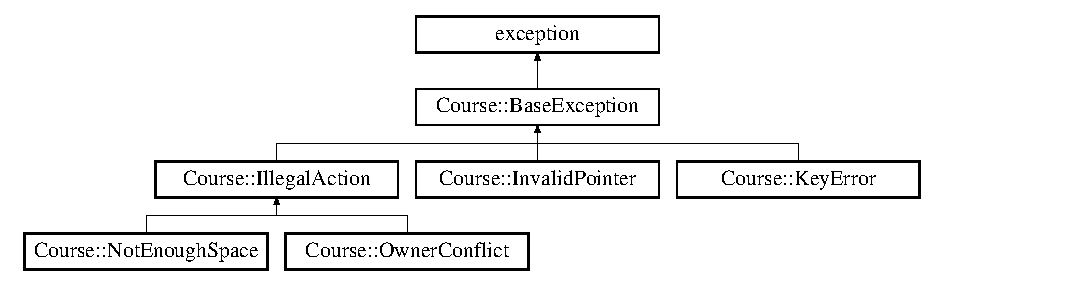
\includegraphics[height=3.393939cm]{classCourse_1_1BaseException}
\end{center}
\end{figure}
\subsection*{Public Member Functions}
\begin{DoxyCompactItemize}
\item 
\hyperlink{classCourse_1_1BaseException_a1d853799191742f9b262fadd69d21b09}{Base\-Exception} (const std\-::string \&\hyperlink{classCourse_1_1BaseException_ac5a744a6af6f2ba9198b58e52bb62f5a}{msg}=\char`\"{}\char`\"{})
\begin{DoxyCompactList}\small\item\em Exception Constructor. \end{DoxyCompactList}\item 
virtual \hyperlink{classCourse_1_1BaseException_a23f96d764abe5a28039bb82a655a484c}{$\sim$\-Base\-Exception} ()=default
\begin{DoxyCompactList}\small\item\em $\sim$\-Exception Default destructor \end{DoxyCompactList}\item 
virtual std\-::string \hyperlink{classCourse_1_1BaseException_ac5a744a6af6f2ba9198b58e52bb62f5a}{msg} () const 
\begin{DoxyCompactList}\small\item\em msg Returns the message being stored in Exception. \end{DoxyCompactList}\end{DoxyCompactItemize}
\subsection*{Private Attributes}
\begin{DoxyCompactItemize}
\item 
const std\-::string \hyperlink{classCourse_1_1BaseException_a31bae6b9817b63c567328da359fd0707}{m\-\_\-msg}
\end{DoxyCompactItemize}


\subsection{Detailed Description}
The Exception class is a base-\/class for custom exceptions in project. 

\subsection{Constructor \& Destructor Documentation}
\hypertarget{classCourse_1_1BaseException_a1d853799191742f9b262fadd69d21b09}{\index{Course\-::\-Base\-Exception@{Course\-::\-Base\-Exception}!Base\-Exception@{Base\-Exception}}
\index{Base\-Exception@{Base\-Exception}!Course::BaseException@{Course\-::\-Base\-Exception}}
\subsubsection[{Base\-Exception}]{\setlength{\rightskip}{0pt plus 5cm}Course\-::\-Base\-Exception\-::\-Base\-Exception (
\begin{DoxyParamCaption}
\item[{const std\-::string \&}]{msg = {\ttfamily \char`\"{}\char`\"{}}}
\end{DoxyParamCaption}
)\hspace{0.3cm}{\ttfamily [inline]}, {\ttfamily [explicit]}}}\label{classCourse_1_1BaseException_a1d853799191742f9b262fadd69d21b09}


Exception Constructor. 


\begin{DoxyParams}{Parameters}
{\em msg} & std\-::string describing the reason for exception. \\
\hline
\end{DoxyParams}
\hypertarget{classCourse_1_1BaseException_a23f96d764abe5a28039bb82a655a484c}{\index{Course\-::\-Base\-Exception@{Course\-::\-Base\-Exception}!$\sim$\-Base\-Exception@{$\sim$\-Base\-Exception}}
\index{$\sim$\-Base\-Exception@{$\sim$\-Base\-Exception}!Course::BaseException@{Course\-::\-Base\-Exception}}
\subsubsection[{$\sim$\-Base\-Exception}]{\setlength{\rightskip}{0pt plus 5cm}virtual Course\-::\-Base\-Exception\-::$\sim$\-Base\-Exception (
\begin{DoxyParamCaption}
{}
\end{DoxyParamCaption}
)\hspace{0.3cm}{\ttfamily [virtual]}, {\ttfamily [default]}}}\label{classCourse_1_1BaseException_a23f96d764abe5a28039bb82a655a484c}


$\sim$\-Exception Default destructor 



\subsection{Member Function Documentation}
\hypertarget{classCourse_1_1BaseException_ac5a744a6af6f2ba9198b58e52bb62f5a}{\index{Course\-::\-Base\-Exception@{Course\-::\-Base\-Exception}!msg@{msg}}
\index{msg@{msg}!Course::BaseException@{Course\-::\-Base\-Exception}}
\subsubsection[{msg}]{\setlength{\rightskip}{0pt plus 5cm}virtual std\-::string Course\-::\-Base\-Exception\-::msg (
\begin{DoxyParamCaption}
{}
\end{DoxyParamCaption}
) const\hspace{0.3cm}{\ttfamily [inline]}, {\ttfamily [virtual]}}}\label{classCourse_1_1BaseException_ac5a744a6af6f2ba9198b58e52bb62f5a}


msg Returns the message being stored in Exception. 

\begin{DoxyReturn}{Returns}
Stored message or empty string. 
\end{DoxyReturn}


\subsection{Member Data Documentation}
\hypertarget{classCourse_1_1BaseException_a31bae6b9817b63c567328da359fd0707}{\index{Course\-::\-Base\-Exception@{Course\-::\-Base\-Exception}!m\-\_\-msg@{m\-\_\-msg}}
\index{m\-\_\-msg@{m\-\_\-msg}!Course::BaseException@{Course\-::\-Base\-Exception}}
\subsubsection[{m\-\_\-msg}]{\setlength{\rightskip}{0pt plus 5cm}const std\-::string Course\-::\-Base\-Exception\-::m\-\_\-msg\hspace{0.3cm}{\ttfamily [private]}}}\label{classCourse_1_1BaseException_a31bae6b9817b63c567328da359fd0707}


The documentation for this class was generated from the following file\-:\begin{DoxyCompactItemize}
\item 
Course/\-Course\-Lib/exceptions/\hyperlink{baseexception_8h}{baseexception.\-h}\end{DoxyCompactItemize}

\hypertarget{classCourse_1_1BasicWorker}{\section{Course\-:\-:Basic\-Worker Class Reference}
\label{classCourse_1_1BasicWorker}\index{Course\-::\-Basic\-Worker@{Course\-::\-Basic\-Worker}}
}


The \hyperlink{classCourse_1_1BasicWorker}{Basic\-Worker} class represents a \char`\"{}normal worker\char`\"{} in the game.  




{\ttfamily \#include $<$basicworker.\-h$>$}

Inheritance diagram for Course\-:\-:Basic\-Worker\-:\begin{figure}[H]
\begin{center}
\leavevmode
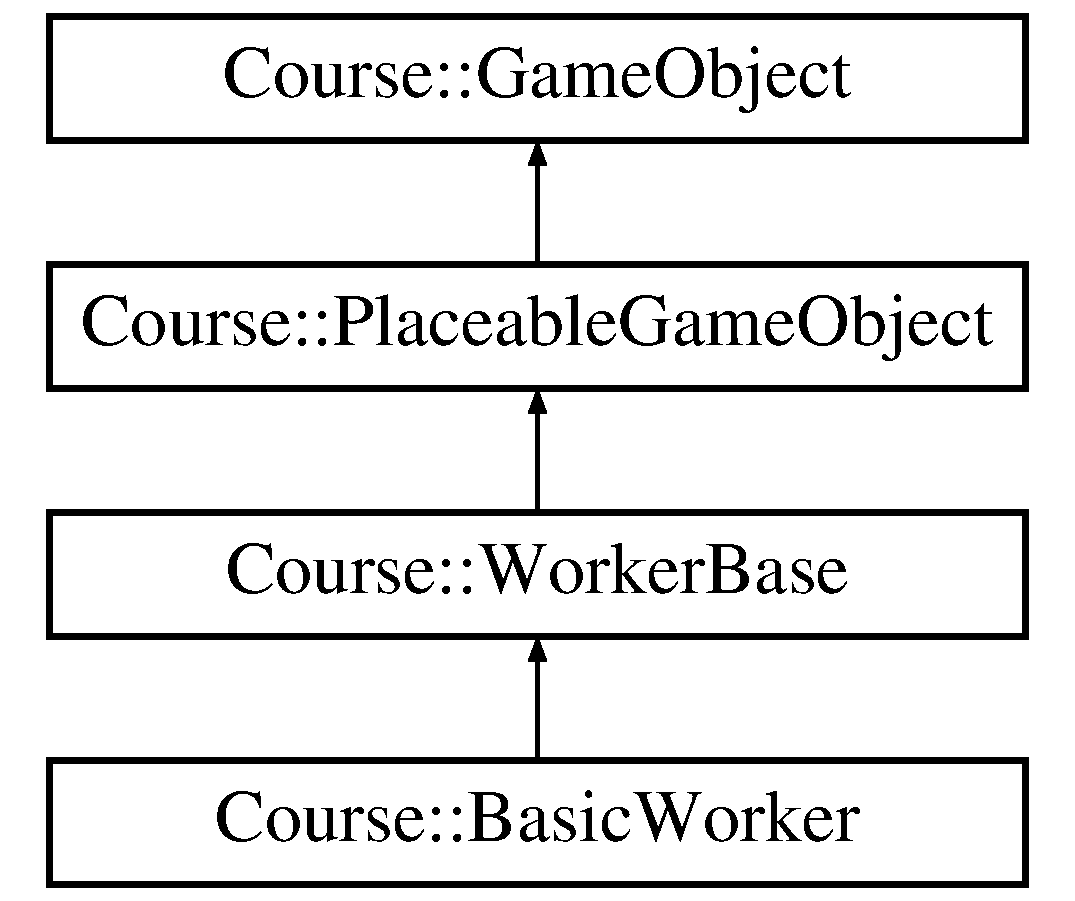
\includegraphics[height=4.000000cm]{classCourse_1_1BasicWorker}
\end{center}
\end{figure}
\subsection*{Public Member Functions}
\begin{DoxyCompactItemize}
\item 
\hyperlink{classCourse_1_1BasicWorker_a066d86fca7e3f10e9ff2bd9f0a2167ff}{Basic\-Worker} ()=delete
\begin{DoxyCompactList}\small\item\em Disabled parameterless constructor. \end{DoxyCompactList}\item 
\hyperlink{classCourse_1_1BasicWorker_a12b697d8a194c9f1a572b93d4e3c40d5}{Basic\-Worker} (const std\-::shared\-\_\-ptr$<$ \hyperlink{classCourse_1_1iGameEventHandler}{i\-Game\-Event\-Handler} $>$ \&eventhandler, const std\-::shared\-\_\-ptr$<$ \hyperlink{classCourse_1_1iObjectManager}{i\-Object\-Manager} $>$ \&objectmanager, const std\-::shared\-\_\-ptr$<$ \hyperlink{classCourse_1_1PlayerBase}{Player\-Base} $>$ \&owner, const int \&tilespaces=1, const \hyperlink{namespaceCourse_ab9a46ed9cd00485e318e5731ea2f78d9}{Resource\-Map} \&cost=\hyperlink{namespaceCourse_1_1ConstResourceMaps_a74eb093a146d0a0d2bfe74ca806e36c2}{Const\-Resource\-Maps\-::\-B\-W\-\_\-\-R\-E\-C\-R\-U\-I\-T\-M\-E\-N\-T\-\_\-\-C\-O\-S\-T}, const \hyperlink{namespaceCourse_a0b96bae1a664dde34efbb1b42dea615e}{Resource\-Map\-Double} \&efficiency=\hyperlink{namespaceCourse_1_1ConstResourceMaps_a895601aa763ac51bf37a0f640eb36c08}{Const\-Resource\-Maps\-::\-B\-W\-\_\-\-W\-O\-R\-K\-E\-R\-\_\-\-E\-F\-F\-I\-C\-I\-E\-N\-C\-Y})
\begin{DoxyCompactList}\small\item\em Constructor for the class. \end{DoxyCompactList}\item 
virtual \hyperlink{classCourse_1_1BasicWorker_a4738d8d4a6c88054355bdd972e1b7aad}{$\sim$\-Basic\-Worker} ()=default
\begin{DoxyCompactList}\small\item\em Default destructor. \end{DoxyCompactList}\item 
virtual std\-::string \hyperlink{classCourse_1_1BasicWorker_a8396e00dafd128cbb86e479296d75c12}{get\-Type} () const override
\begin{DoxyCompactList}\small\item\em get\-Type Returns a string describing objects type. This should be overriden in each inherited class. Makes checking object's type easier for students. \end{DoxyCompactList}\item 
virtual bool \hyperlink{classCourse_1_1BasicWorker_ab12d85004e92d9a1e85396d72c6cac98}{can\-Be\-Placed\-On\-Tile} (const std\-::shared\-\_\-ptr$<$ \hyperlink{classCourse_1_1TileBase}{Tile\-Base} $>$ \&target) const override
\begin{DoxyCompactList}\small\item\em Check if the worker can be placed on the Tile according to it's placement rule. Only rule is that the Tile must have same owner as the worker. \end{DoxyCompactList}\item 
virtual void \hyperlink{classCourse_1_1BasicWorker_a626bab94f45602a34631c7ab6e60d829}{do\-Special\-Action} () override
\begin{DoxyCompactList}\small\item\em Performs the Worker's default action. \end{DoxyCompactList}\item 
virtual const \hyperlink{namespaceCourse_a0b96bae1a664dde34efbb1b42dea615e}{Resource\-Map\-Double} \hyperlink{classCourse_1_1BasicWorker_a870cf500ea86d30db583ce64299d9df4}{tile\-Work\-Action} () override
\begin{DoxyCompactList}\small\item\em Returns Worker's efficiency at resource production. Worker consumes F\-O\-O\-D and M\-O\-N\-E\-Y. Resource consumption and resource focus determine final multiplier that is based on W\-O\-R\-K\-E\-R\-\_\-\-E\-F\-F\-I\-C\-I\-E\-N\-C\-Y. \end{DoxyCompactList}\end{DoxyCompactItemize}
\subsection*{Additional Inherited Members}


\subsection{Detailed Description}
The \hyperlink{classCourse_1_1BasicWorker}{Basic\-Worker} class represents a \char`\"{}normal worker\char`\"{} in the game. 

Worker has following production-\/efficiency\-: \par

\begin{DoxyItemize}
\item Money -\/ 0.\-25 \par

\item Food -\/ 1.\-00 \par

\item Wood -\/ 0.\-75 \par

\item Stone -\/ 0.\-50 \par

\item Ore -\/ 0.\-50 \par
 Basic\-Workers consume Food and money. \par

\item 1 Food -\/ Or \hyperlink{classCourse_1_1BasicWorker}{Basic\-Worker} refuses to work. \par

\item 1 Money -\/ Or \hyperlink{classCourse_1_1BasicWorker}{Basic\-Worker} works at 50\% efficiency. \par

\item Resourcefocus adds 25\% efficiency for the focused resource, even if the worker is refusing work. 
\end{DoxyItemize}

\subsection{Constructor \& Destructor Documentation}
\hypertarget{classCourse_1_1BasicWorker_a066d86fca7e3f10e9ff2bd9f0a2167ff}{\index{Course\-::\-Basic\-Worker@{Course\-::\-Basic\-Worker}!Basic\-Worker@{Basic\-Worker}}
\index{Basic\-Worker@{Basic\-Worker}!Course::BasicWorker@{Course\-::\-Basic\-Worker}}
\subsubsection[{Basic\-Worker}]{\setlength{\rightskip}{0pt plus 5cm}Course\-::\-Basic\-Worker\-::\-Basic\-Worker (
\begin{DoxyParamCaption}
{}
\end{DoxyParamCaption}
)\hspace{0.3cm}{\ttfamily [delete]}}}\label{classCourse_1_1BasicWorker_a066d86fca7e3f10e9ff2bd9f0a2167ff}


Disabled parameterless constructor. 

\hypertarget{classCourse_1_1BasicWorker_a12b697d8a194c9f1a572b93d4e3c40d5}{\index{Course\-::\-Basic\-Worker@{Course\-::\-Basic\-Worker}!Basic\-Worker@{Basic\-Worker}}
\index{Basic\-Worker@{Basic\-Worker}!Course::BasicWorker@{Course\-::\-Basic\-Worker}}
\subsubsection[{Basic\-Worker}]{\setlength{\rightskip}{0pt plus 5cm}Course\-::\-Basic\-Worker\-::\-Basic\-Worker (
\begin{DoxyParamCaption}
\item[{const std\-::shared\-\_\-ptr$<$ {\bf i\-Game\-Event\-Handler} $>$ \&}]{eventhandler, }
\item[{const std\-::shared\-\_\-ptr$<$ {\bf i\-Object\-Manager} $>$ \&}]{objectmanager, }
\item[{const std\-::shared\-\_\-ptr$<$ {\bf Player\-Base} $>$ \&}]{owner, }
\item[{const int \&}]{tilespaces = {\ttfamily 1}, }
\item[{const {\bf Resource\-Map} \&}]{cost = {\ttfamily {\bf Const\-Resource\-Maps\-::\-B\-W\-\_\-\-R\-E\-C\-R\-U\-I\-T\-M\-E\-N\-T\-\_\-\-C\-O\-S\-T}}, }
\item[{const {\bf Resource\-Map\-Double} \&}]{efficiency = {\ttfamily {\bf Const\-Resource\-Maps\-::\-B\-W\-\_\-\-W\-O\-R\-K\-E\-R\-\_\-\-E\-F\-F\-I\-C\-I\-E\-N\-C\-Y}}}
\end{DoxyParamCaption}
)}}\label{classCourse_1_1BasicWorker_a12b697d8a194c9f1a572b93d4e3c40d5}


Constructor for the class. 


\begin{DoxyParams}{Parameters}
{\em eventhandler} & points to the student's Game\-Event\-Handler. \\
\hline
{\em owner} & points to the owning player. \\
\hline
{\em descriptions} & contains descriptions and flavor texts. \\
\hline
\end{DoxyParams}
\hypertarget{classCourse_1_1BasicWorker_a4738d8d4a6c88054355bdd972e1b7aad}{\index{Course\-::\-Basic\-Worker@{Course\-::\-Basic\-Worker}!$\sim$\-Basic\-Worker@{$\sim$\-Basic\-Worker}}
\index{$\sim$\-Basic\-Worker@{$\sim$\-Basic\-Worker}!Course::BasicWorker@{Course\-::\-Basic\-Worker}}
\subsubsection[{$\sim$\-Basic\-Worker}]{\setlength{\rightskip}{0pt plus 5cm}virtual Course\-::\-Basic\-Worker\-::$\sim$\-Basic\-Worker (
\begin{DoxyParamCaption}
{}
\end{DoxyParamCaption}
)\hspace{0.3cm}{\ttfamily [virtual]}, {\ttfamily [default]}}}\label{classCourse_1_1BasicWorker_a4738d8d4a6c88054355bdd972e1b7aad}


Default destructor. 



\subsection{Member Function Documentation}
\hypertarget{classCourse_1_1BasicWorker_ab12d85004e92d9a1e85396d72c6cac98}{\index{Course\-::\-Basic\-Worker@{Course\-::\-Basic\-Worker}!can\-Be\-Placed\-On\-Tile@{can\-Be\-Placed\-On\-Tile}}
\index{can\-Be\-Placed\-On\-Tile@{can\-Be\-Placed\-On\-Tile}!Course::BasicWorker@{Course\-::\-Basic\-Worker}}
\subsubsection[{can\-Be\-Placed\-On\-Tile}]{\setlength{\rightskip}{0pt plus 5cm}bool Course\-::\-Basic\-Worker\-::can\-Be\-Placed\-On\-Tile (
\begin{DoxyParamCaption}
\item[{const std\-::shared\-\_\-ptr$<$ {\bf Tile\-Base} $>$ \&}]{target}
\end{DoxyParamCaption}
) const\hspace{0.3cm}{\ttfamily [override]}, {\ttfamily [virtual]}}}\label{classCourse_1_1BasicWorker_ab12d85004e92d9a1e85396d72c6cac98}


Check if the worker can be placed on the Tile according to it's placement rule. Only rule is that the Tile must have same owner as the worker. 


\begin{DoxyParams}{Parameters}
{\em target} & is the Tile that worker is being placed on. \\
\hline
\end{DoxyParams}
\begin{DoxyReturn}{Returns}
True -\/ If baseclass' method return true and target Tile has space for worker. False -\/ If both conditions aren't met. 
\end{DoxyReturn}
\begin{DoxyNote}{Note}
Override to change placement rules for derived worker. 
\end{DoxyNote}
\begin{DoxyPostcond}{Postcondition}
Exception guarantee\-: Basic 
\end{DoxyPostcond}


Reimplemented from \hyperlink{classCourse_1_1WorkerBase_ad80874970ab91bca95b9d3f959e838d2}{Course\-::\-Worker\-Base}.

\hypertarget{classCourse_1_1BasicWorker_a626bab94f45602a34631c7ab6e60d829}{\index{Course\-::\-Basic\-Worker@{Course\-::\-Basic\-Worker}!do\-Special\-Action@{do\-Special\-Action}}
\index{do\-Special\-Action@{do\-Special\-Action}!Course::BasicWorker@{Course\-::\-Basic\-Worker}}
\subsubsection[{do\-Special\-Action}]{\setlength{\rightskip}{0pt plus 5cm}void Course\-::\-Basic\-Worker\-::do\-Special\-Action (
\begin{DoxyParamCaption}
{}
\end{DoxyParamCaption}
)\hspace{0.3cm}{\ttfamily [override]}, {\ttfamily [virtual]}}}\label{classCourse_1_1BasicWorker_a626bab94f45602a34631c7ab6e60d829}


Performs the Worker's default action. 



Implements \hyperlink{classCourse_1_1WorkerBase_a78553f35740e1c07d8f1071b5fc82212}{Course\-::\-Worker\-Base}.

\hypertarget{classCourse_1_1BasicWorker_a8396e00dafd128cbb86e479296d75c12}{\index{Course\-::\-Basic\-Worker@{Course\-::\-Basic\-Worker}!get\-Type@{get\-Type}}
\index{get\-Type@{get\-Type}!Course::BasicWorker@{Course\-::\-Basic\-Worker}}
\subsubsection[{get\-Type}]{\setlength{\rightskip}{0pt plus 5cm}std\-::string Course\-::\-Basic\-Worker\-::get\-Type (
\begin{DoxyParamCaption}
{}
\end{DoxyParamCaption}
) const\hspace{0.3cm}{\ttfamily [override]}, {\ttfamily [virtual]}}}\label{classCourse_1_1BasicWorker_a8396e00dafd128cbb86e479296d75c12}


get\-Type Returns a string describing objects type. This should be overriden in each inherited class. Makes checking object's type easier for students. 

\begin{DoxyReturn}{Returns}
std\-::string that represents Object's type. 
\end{DoxyReturn}
\begin{DoxyPostcond}{Postcondition}
Exception guarantee\-: No-\/throw 
\end{DoxyPostcond}
\begin{DoxyNote}{Note}
You can use this in e.\-g. debugging and similar printing. 
\end{DoxyNote}


Reimplemented from \hyperlink{classCourse_1_1WorkerBase_afe6049810eec47fffe2c2a7334564ef9}{Course\-::\-Worker\-Base}.

\hypertarget{classCourse_1_1BasicWorker_a870cf500ea86d30db583ce64299d9df4}{\index{Course\-::\-Basic\-Worker@{Course\-::\-Basic\-Worker}!tile\-Work\-Action@{tile\-Work\-Action}}
\index{tile\-Work\-Action@{tile\-Work\-Action}!Course::BasicWorker@{Course\-::\-Basic\-Worker}}
\subsubsection[{tile\-Work\-Action}]{\setlength{\rightskip}{0pt plus 5cm}const {\bf Resource\-Map\-Double} Course\-::\-Basic\-Worker\-::tile\-Work\-Action (
\begin{DoxyParamCaption}
{}
\end{DoxyParamCaption}
)\hspace{0.3cm}{\ttfamily [override]}, {\ttfamily [virtual]}}}\label{classCourse_1_1BasicWorker_a870cf500ea86d30db583ce64299d9df4}


Returns Worker's efficiency at resource production. Worker consumes F\-O\-O\-D and M\-O\-N\-E\-Y. Resource consumption and resource focus determine final multiplier that is based on W\-O\-R\-K\-E\-R\-\_\-\-E\-F\-F\-I\-C\-I\-E\-N\-C\-Y. 

\begin{DoxyReturn}{Returns}

\end{DoxyReturn}


Reimplemented from \hyperlink{classCourse_1_1WorkerBase_af0c1bb4f3bbea015e2a55aa6eff7f9ae}{Course\-::\-Worker\-Base}.



The documentation for this class was generated from the following files\-:\begin{DoxyCompactItemize}
\item 
Course/\-Course\-Lib/workers/\hyperlink{basicworker_8h}{basicworker.\-h}\item 
Course/\-Course\-Lib/workers/\hyperlink{basicworker_8cpp}{basicworker.\-cpp}\end{DoxyCompactItemize}

\hypertarget{classbegindialog}{\section{begindialog Class Reference}
\label{classbegindialog}\index{begindialog@{begindialog}}
}


The begindialog class shows pop-\/up window in the beginning of the game. Asks \par
for player names, amount of starting resources and amount of resources to win.  




{\ttfamily \#include $<$begindialog.\-hh$>$}

Inheritance diagram for begindialog\-:\begin{figure}[H]
\begin{center}
\leavevmode
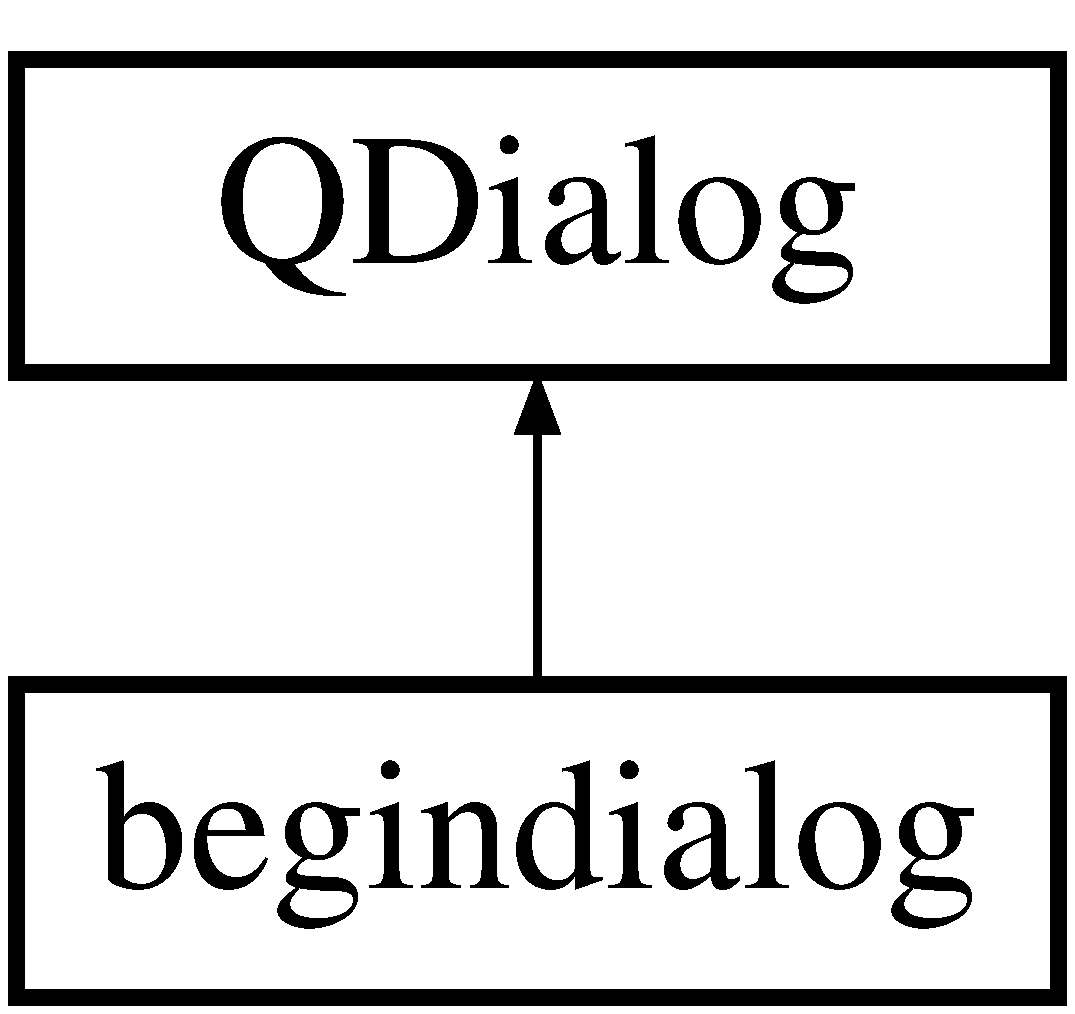
\includegraphics[height=2.000000cm]{classbegindialog}
\end{center}
\end{figure}
\subsection*{Public Member Functions}
\begin{DoxyCompactItemize}
\item 
\hyperlink{classbegindialog_a76bb9418e0b00fbb94c2cef459a83b08}{begindialog} (Q\-Widget $\ast$parent=0)
\begin{DoxyCompactList}\small\item\em Constructor for the class. \end{DoxyCompactList}\item 
\hyperlink{classbegindialog_a83236454b5fab5d4fee1ef0c6f0307eb}{$\sim$begindialog} ()
\item 
std\-::vector$<$ std\-::string $>$ \hyperlink{classbegindialog_a3614bf1959c37603e094d39640190123}{get\-Playernames} ()
\begin{DoxyCompactList}\small\item\em get\-Playernames Returns players names. \end{DoxyCompactList}\item 
\hyperlink{namespaceCourse_ab9a46ed9cd00485e318e5731ea2f78d9}{Course\-::\-Resource\-Map} \hyperlink{classbegindialog_a1fdc4bd90ddc27df8064bea149b14fbf}{get\-Starting\-Resources} ()
\begin{DoxyCompactList}\small\item\em get\-Starting\-Resources Returns amount of starting resources. \end{DoxyCompactList}\item 
int \hyperlink{classbegindialog_a0a0d98c8c33dc11b35293a9d6104e2d6}{get\-Resources\-To\-Win} ()
\begin{DoxyCompactList}\small\item\em get\-Resources\-To\-Win Returns amount of resources needed for a win. \end{DoxyCompactList}\end{DoxyCompactItemize}
\subsection*{Private Attributes}
\begin{DoxyCompactItemize}
\item 
Ui\-::begindialog $\ast$ \hyperlink{classbegindialog_a055ab69448a9247db34df24a4c0abddc}{ui}
\end{DoxyCompactItemize}


\subsection{Detailed Description}
The begindialog class shows pop-\/up window in the beginning of the game. Asks \par
for player names, amount of starting resources and amount of resources to win. 

\subsection{Constructor \& Destructor Documentation}
\hypertarget{classbegindialog_a76bb9418e0b00fbb94c2cef459a83b08}{\index{begindialog@{begindialog}!begindialog@{begindialog}}
\index{begindialog@{begindialog}!begindialog@{begindialog}}
\subsubsection[{begindialog}]{\setlength{\rightskip}{0pt plus 5cm}begindialog\-::begindialog (
\begin{DoxyParamCaption}
\item[{Q\-Widget $\ast$}]{parent = {\ttfamily 0}}
\end{DoxyParamCaption}
)\hspace{0.3cm}{\ttfamily [explicit]}}}\label{classbegindialog_a76bb9418e0b00fbb94c2cef459a83b08}


Constructor for the class. 


\begin{DoxyParams}{Parameters}
{\em parent} & can be used to point to a parent widget. Not used. \\
\hline
\end{DoxyParams}
\hypertarget{classbegindialog_a83236454b5fab5d4fee1ef0c6f0307eb}{\index{begindialog@{begindialog}!$\sim$begindialog@{$\sim$begindialog}}
\index{$\sim$begindialog@{$\sim$begindialog}!begindialog@{begindialog}}
\subsubsection[{$\sim$begindialog}]{\setlength{\rightskip}{0pt plus 5cm}begindialog\-::$\sim$begindialog (
\begin{DoxyParamCaption}
{}
\end{DoxyParamCaption}
)}}\label{classbegindialog_a83236454b5fab5d4fee1ef0c6f0307eb}


\subsection{Member Function Documentation}
\hypertarget{classbegindialog_a3614bf1959c37603e094d39640190123}{\index{begindialog@{begindialog}!get\-Playernames@{get\-Playernames}}
\index{get\-Playernames@{get\-Playernames}!begindialog@{begindialog}}
\subsubsection[{get\-Playernames}]{\setlength{\rightskip}{0pt plus 5cm}std\-::vector$<$ std\-::string $>$ begindialog\-::get\-Playernames (
\begin{DoxyParamCaption}
{}
\end{DoxyParamCaption}
)}}\label{classbegindialog_a3614bf1959c37603e094d39640190123}


get\-Playernames Returns players names. 

\begin{DoxyReturn}{Returns}
Vector of containing both player names. 
\end{DoxyReturn}
\hypertarget{classbegindialog_a0a0d98c8c33dc11b35293a9d6104e2d6}{\index{begindialog@{begindialog}!get\-Resources\-To\-Win@{get\-Resources\-To\-Win}}
\index{get\-Resources\-To\-Win@{get\-Resources\-To\-Win}!begindialog@{begindialog}}
\subsubsection[{get\-Resources\-To\-Win}]{\setlength{\rightskip}{0pt plus 5cm}int begindialog\-::get\-Resources\-To\-Win (
\begin{DoxyParamCaption}
{}
\end{DoxyParamCaption}
)}}\label{classbegindialog_a0a0d98c8c33dc11b35293a9d6104e2d6}


get\-Resources\-To\-Win Returns amount of resources needed for a win. 

\begin{DoxyReturn}{Returns}
Amount of resources needed for a win. 
\end{DoxyReturn}
\hypertarget{classbegindialog_a1fdc4bd90ddc27df8064bea149b14fbf}{\index{begindialog@{begindialog}!get\-Starting\-Resources@{get\-Starting\-Resources}}
\index{get\-Starting\-Resources@{get\-Starting\-Resources}!begindialog@{begindialog}}
\subsubsection[{get\-Starting\-Resources}]{\setlength{\rightskip}{0pt plus 5cm}{\bf Course\-::\-Resource\-Map} begindialog\-::get\-Starting\-Resources (
\begin{DoxyParamCaption}
{}
\end{DoxyParamCaption}
)}}\label{classbegindialog_a1fdc4bd90ddc27df8064bea149b14fbf}


get\-Starting\-Resources Returns amount of starting resources. 

\begin{DoxyReturn}{Returns}
Resource\-Map containing amounts of resources. 
\end{DoxyReturn}


\subsection{Member Data Documentation}
\hypertarget{classbegindialog_a055ab69448a9247db34df24a4c0abddc}{\index{begindialog@{begindialog}!ui@{ui}}
\index{ui@{ui}!begindialog@{begindialog}}
\subsubsection[{ui}]{\setlength{\rightskip}{0pt plus 5cm}Ui\-::begindialog$\ast$ begindialog\-::ui\hspace{0.3cm}{\ttfamily [private]}}}\label{classbegindialog_a055ab69448a9247db34df24a4c0abddc}


The documentation for this class was generated from the following files\-:\begin{DoxyCompactItemize}
\item 
Game/ui/\hyperlink{begindialog_8hh}{begindialog.\-hh}\item 
Game/ui/\hyperlink{begindialog_8cpp}{begindialog.\-cpp}\end{DoxyCompactItemize}

\hypertarget{classGame_1_1Blockfield}{\section{Game\-:\-:Blockfield Class Reference}
\label{classGame_1_1Blockfield}\index{Game\-::\-Blockfield@{Game\-::\-Blockfield}}
}


The \hyperlink{classGame_1_1Blockfield}{Blockfield} class represents a blockfield in the gameworld.  




{\ttfamily \#include $<$blockfield.\-h$>$}

Inheritance diagram for Game\-:\-:Blockfield\-:\begin{figure}[H]
\begin{center}
\leavevmode
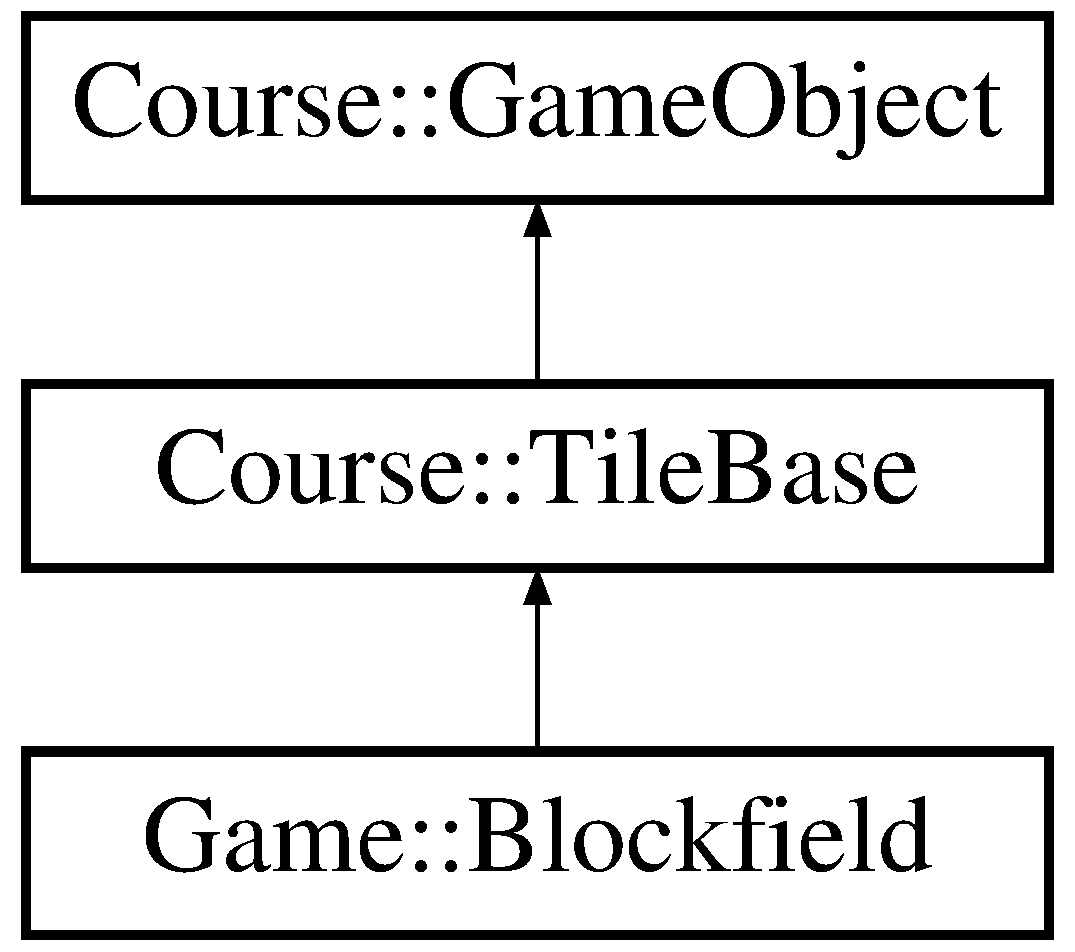
\includegraphics[height=3.000000cm]{classGame_1_1Blockfield}
\end{center}
\end{figure}
\subsection*{Public Member Functions}
\begin{DoxyCompactItemize}
\item 
\hyperlink{classGame_1_1Blockfield_a7970ee32ecccf5c3b81e71a4c4554375}{Blockfield} ()=delete
\begin{DoxyCompactList}\small\item\em Disabled parameterless constructor. \end{DoxyCompactList}\item 
\hyperlink{classGame_1_1Blockfield_a103d7f67c9c7ae2a20f04d8d785ad6ad}{Blockfield} (const \hyperlink{classCourse_1_1Coordinate}{Course\-::\-Coordinate} \&location, const std\-::shared\-\_\-ptr$<$ \hyperlink{classCourse_1_1iGameEventHandler}{Course\-::i\-Game\-Event\-Handler} $>$ \&eventhandler, const std\-::shared\-\_\-ptr$<$ \hyperlink{classCourse_1_1iObjectManager}{Course\-::i\-Object\-Manager} $>$ \&objectmanager, const unsigned int \&max\-\_\-build=3, const unsigned int \&max\-\_\-work=3, const \hyperlink{namespaceCourse_ab9a46ed9cd00485e318e5731ea2f78d9}{Course\-::\-Resource\-Map} \&production=\hyperlink{namespaceGame_1_1ConstResourceMaps_aca102e5c0cc70c09b1934a785bca2b91}{Game\-::\-Const\-Resource\-Maps\-::\-B\-L\-O\-C\-K\-F\-I\-E\-L\-D\-\_\-\-B\-P})
\begin{DoxyCompactList}\small\item\em Constructor for the class. \end{DoxyCompactList}\item 
virtual \hyperlink{classGame_1_1Blockfield_abeea15b0150fd65a357dce47e09131eb}{$\sim$\-Blockfield} ()=default
\begin{DoxyCompactList}\small\item\em Default destructor. \end{DoxyCompactList}\item 
virtual std\-::string \hyperlink{classGame_1_1Blockfield_af5e2a4c262cb1f59e442b60c8404b715}{get\-Type} () const override
\item 
void \hyperlink{classGame_1_1Blockfield_a7b6ecdadde2797965d6fbbe640d664bc}{add\-Building} (const std\-::shared\-\_\-ptr$<$ \hyperlink{classCourse_1_1BuildingBase}{Course\-::\-Building\-Base} $>$ \&building) override
\begin{DoxyCompactList}\small\item\em Adds a new building-\/object to the tile. Building in blockfield adds one hold-\/marker to the building. \end{DoxyCompactList}\end{DoxyCompactItemize}
\subsection*{Additional Inherited Members}


\subsection{Detailed Description}
The \hyperlink{classGame_1_1Blockfield}{Blockfield} class represents a blockfield in the gameworld. 

\hyperlink{classGame_1_1Blockfield}{Blockfield} has Basic\-Production\-: \par

\begin{DoxyItemize}
\item Money = 2
\item Food = 0
\item Wood = 0
\item Stone = 5
\item Ore = 2
\end{DoxyItemize}

Building in the blockfield takes time. So buildings get extra hold-\/marker.

Tile supports 3 buildings. 

\subsection{Constructor \& Destructor Documentation}
\hypertarget{classGame_1_1Blockfield_a7970ee32ecccf5c3b81e71a4c4554375}{\index{Game\-::\-Blockfield@{Game\-::\-Blockfield}!Blockfield@{Blockfield}}
\index{Blockfield@{Blockfield}!Game::Blockfield@{Game\-::\-Blockfield}}
\subsubsection[{Blockfield}]{\setlength{\rightskip}{0pt plus 5cm}Game\-::\-Blockfield\-::\-Blockfield (
\begin{DoxyParamCaption}
{}
\end{DoxyParamCaption}
)\hspace{0.3cm}{\ttfamily [delete]}}}\label{classGame_1_1Blockfield_a7970ee32ecccf5c3b81e71a4c4554375}


Disabled parameterless constructor. 

\hypertarget{classGame_1_1Blockfield_a103d7f67c9c7ae2a20f04d8d785ad6ad}{\index{Game\-::\-Blockfield@{Game\-::\-Blockfield}!Blockfield@{Blockfield}}
\index{Blockfield@{Blockfield}!Game::Blockfield@{Game\-::\-Blockfield}}
\subsubsection[{Blockfield}]{\setlength{\rightskip}{0pt plus 5cm}Game\-::\-Blockfield\-::\-Blockfield (
\begin{DoxyParamCaption}
\item[{const {\bf Course\-::\-Coordinate} \&}]{location, }
\item[{const std\-::shared\-\_\-ptr$<$ {\bf Course\-::i\-Game\-Event\-Handler} $>$ \&}]{eventhandler, }
\item[{const std\-::shared\-\_\-ptr$<$ {\bf Course\-::i\-Object\-Manager} $>$ \&}]{objectmanager, }
\item[{const unsigned int \&}]{max\-\_\-build = {\ttfamily 3}, }
\item[{const unsigned int \&}]{max\-\_\-work = {\ttfamily 3}, }
\item[{const {\bf Course\-::\-Resource\-Map} \&}]{production = {\ttfamily {\bf Game\-::\-Const\-Resource\-Maps\-::\-B\-L\-O\-C\-K\-F\-I\-E\-L\-D\-\_\-\-B\-P}}}
\end{DoxyParamCaption}
)}}\label{classGame_1_1Blockfield_a103d7f67c9c7ae2a20f04d8d785ad6ad}


Constructor for the class. 


\begin{DoxyParams}{Parameters}
{\em location} & is the Coordinate where the Tile is located in the game. \\
\hline
{\em eventhandler} & points to the \hyperlink{classGame_1_1GameEventHandler}{Game\-Event\-Handler}. \\
\hline
{\em objectmanager} & points to the \hyperlink{classGame_1_1ObjectManager}{Object\-Manager}. \\
\hline
{\em max\-\_\-build} & defines maximum amount of buildings on the tile \\
\hline
{\em max\-\_\-work} & defines maximum amount of workers on the tile \\
\hline
{\em production} & sets the tiles production \\
\hline
\end{DoxyParams}
\hypertarget{classGame_1_1Blockfield_abeea15b0150fd65a357dce47e09131eb}{\index{Game\-::\-Blockfield@{Game\-::\-Blockfield}!$\sim$\-Blockfield@{$\sim$\-Blockfield}}
\index{$\sim$\-Blockfield@{$\sim$\-Blockfield}!Game::Blockfield@{Game\-::\-Blockfield}}
\subsubsection[{$\sim$\-Blockfield}]{\setlength{\rightskip}{0pt plus 5cm}virtual Game\-::\-Blockfield\-::$\sim$\-Blockfield (
\begin{DoxyParamCaption}
{}
\end{DoxyParamCaption}
)\hspace{0.3cm}{\ttfamily [virtual]}, {\ttfamily [default]}}}\label{classGame_1_1Blockfield_abeea15b0150fd65a357dce47e09131eb}


Default destructor. 



\subsection{Member Function Documentation}
\hypertarget{classGame_1_1Blockfield_a7b6ecdadde2797965d6fbbe640d664bc}{\index{Game\-::\-Blockfield@{Game\-::\-Blockfield}!add\-Building@{add\-Building}}
\index{add\-Building@{add\-Building}!Game::Blockfield@{Game\-::\-Blockfield}}
\subsubsection[{add\-Building}]{\setlength{\rightskip}{0pt plus 5cm}void Game\-::\-Blockfield\-::add\-Building (
\begin{DoxyParamCaption}
\item[{const std\-::shared\-\_\-ptr$<$ {\bf Course\-::\-Building\-Base} $>$ \&}]{building}
\end{DoxyParamCaption}
)\hspace{0.3cm}{\ttfamily [override]}, {\ttfamily [virtual]}}}\label{classGame_1_1Blockfield_a7b6ecdadde2797965d6fbbe640d664bc}


Adds a new building-\/object to the tile. Building in blockfield adds one hold-\/marker to the building. 

Phases\-: \par

\begin{DoxyEnumerate}
\item Check that there is space for the building. \par

\item Call parent's add\-Building \par

\item Add a Hold\-Marker for the building. \par
 \begin{DoxyPostcond}{Postcondition}
Exception guarantee\-: Strong 
\end{DoxyPostcond}

\begin{DoxyExceptions}{Exceptions}
{\em Owner\-Conflict} & -\/ If the tile's ownership prevents placing the {\bfseries building}. \\
\hline
{\em No\-Space} & -\/ If the tile doesn't have enough space for the {\bfseries building}. \\
\hline
\end{DoxyExceptions}

\end{DoxyEnumerate}

Reimplemented from \hyperlink{classCourse_1_1TileBase_add69a1e9ec009dedb28ce54c8535370b}{Course\-::\-Tile\-Base}.

\hypertarget{classGame_1_1Blockfield_af5e2a4c262cb1f59e442b60c8404b715}{\index{Game\-::\-Blockfield@{Game\-::\-Blockfield}!get\-Type@{get\-Type}}
\index{get\-Type@{get\-Type}!Game::Blockfield@{Game\-::\-Blockfield}}
\subsubsection[{get\-Type}]{\setlength{\rightskip}{0pt plus 5cm}std\-::string Game\-::\-Blockfield\-::get\-Type (
\begin{DoxyParamCaption}
{}
\end{DoxyParamCaption}
) const\hspace{0.3cm}{\ttfamily [override]}, {\ttfamily [virtual]}}}\label{classGame_1_1Blockfield_af5e2a4c262cb1f59e442b60c8404b715}






Reimplemented from \hyperlink{classCourse_1_1TileBase_af1a8aaa3407ad3ade7ffe8f2fb421288}{Course\-::\-Tile\-Base}.



The documentation for this class was generated from the following files\-:\begin{DoxyCompactItemize}
\item 
Game/tiles/\hyperlink{blockfield_8h}{blockfield.\-h}\item 
Game/tiles/\hyperlink{blockfield_8cpp}{blockfield.\-cpp}\end{DoxyCompactItemize}

\hypertarget{classCourse_1_1BuildingBase}{\section{Course\-:\-:Building\-Base Class Reference}
\label{classCourse_1_1BuildingBase}\index{Course\-::\-Building\-Base@{Course\-::\-Building\-Base}}
}


The \hyperlink{classCourse_1_1BuildingBase}{Building\-Base} class is a base-\/class for different buildings in the game.  




{\ttfamily \#include $<$buildingbase.\-h$>$}

Inheritance diagram for Course\-:\-:Building\-Base\-:\begin{figure}[H]
\begin{center}
\leavevmode
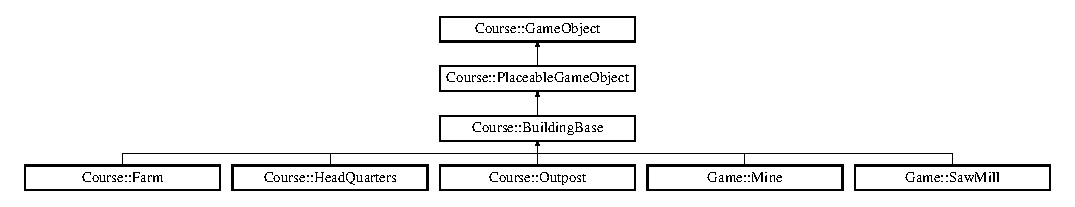
\includegraphics[height=2.333333cm]{classCourse_1_1BuildingBase}
\end{center}
\end{figure}
\subsection*{Public Member Functions}
\begin{DoxyCompactItemize}
\item 
\hyperlink{classCourse_1_1BuildingBase_a899534ce249e7bd1c55883b7c0f4db93}{Building\-Base} ()=delete
\begin{DoxyCompactList}\small\item\em Disabled parameterless constructor. \end{DoxyCompactList}\item 
\hyperlink{classCourse_1_1BuildingBase_a2aefafd40f901b002c09c2561fe4327c}{Building\-Base} (const std\-::shared\-\_\-ptr$<$ \hyperlink{classCourse_1_1iGameEventHandler}{i\-Game\-Event\-Handler} $>$ \&eventhandler, const std\-::shared\-\_\-ptr$<$ \hyperlink{classCourse_1_1iObjectManager}{i\-Object\-Manager} $>$ \&objectmanager, const std\-::shared\-\_\-ptr$<$ \hyperlink{classCourse_1_1PlayerBase}{Player\-Base} $>$ \&owner, const int \&tilespaces=1, const \hyperlink{namespaceCourse_ab9a46ed9cd00485e318e5731ea2f78d9}{Resource\-Map} \&buildcost=\{\}, const \hyperlink{namespaceCourse_ab9a46ed9cd00485e318e5731ea2f78d9}{Resource\-Map} \&production=\{\})
\begin{DoxyCompactList}\small\item\em Constructor for the class. \end{DoxyCompactList}\item 
virtual \hyperlink{classCourse_1_1BuildingBase_aa1787cfb58ab07902c29fe02941dced6}{$\sim$\-Building\-Base} ()=default
\begin{DoxyCompactList}\small\item\em Default destructor. \end{DoxyCompactList}\item 
virtual std\-::string \hyperlink{classCourse_1_1BuildingBase_ac2cc44e08dc73d05b1617bf71295baaf}{get\-Type} () const override
\begin{DoxyCompactList}\small\item\em get\-Type Returns a string describing objects type. This should be overriden in each inherited class. Makes checking object's type easier for students. \end{DoxyCompactList}\item 
virtual void \hyperlink{classCourse_1_1BuildingBase_aa7363afb8cb5163db548e982bb3e9934}{do\-Special\-Action} ()
\begin{DoxyCompactList}\small\item\em Performs building's default action. \end{DoxyCompactList}\item 
virtual void \hyperlink{classCourse_1_1BuildingBase_a2e3a5ad53afb74fdf030a5679e40a341}{on\-Build\-Action} ()
\begin{DoxyCompactList}\small\item\em Performs building's possible action after construction. \end{DoxyCompactList}\item 
virtual \hyperlink{namespaceCourse_ab9a46ed9cd00485e318e5731ea2f78d9}{Resource\-Map} \hyperlink{classCourse_1_1BuildingBase_ad53ecc1dea91e3ca51c31759fe1680cb}{get\-Production} ()
\begin{DoxyCompactList}\small\item\em Return's building's production as a Resource\-Map.\par
. \end{DoxyCompactList}\item 
virtual void \hyperlink{classCourse_1_1BuildingBase_aaa5fb119b7a1873744b83900b3ce04d2}{add\-Hold\-Markers} (int amount) final
\begin{DoxyCompactList}\small\item\em Adds the amount to hold-\/markers. \end{DoxyCompactList}\item 
virtual int \hyperlink{classCourse_1_1BuildingBase_afa4f0dd0fdfaf9b600d10fe477080cf6}{hold\-Count} () const final
\begin{DoxyCompactList}\small\item\em Returns the amount of hold-\/markers. \end{DoxyCompactList}\item 
virtual bool \hyperlink{classCourse_1_1BuildingBase_add23c593f509f39654f2d5abc7d8c072}{can\-Be\-Placed\-On\-Tile} (const std\-::shared\-\_\-ptr$<$ \hyperlink{classCourse_1_1TileBase}{Tile\-Base} $>$ \&target) const override
\begin{DoxyCompactList}\small\item\em Returns boolean based on wheter the building can or can't be placed on a Tile-\/object. \end{DoxyCompactList}\end{DoxyCompactItemize}
\subsection*{Public Attributes}
\begin{DoxyCompactItemize}
\item 
const \hyperlink{namespaceCourse_ab9a46ed9cd00485e318e5731ea2f78d9}{Resource\-Map} \hyperlink{classCourse_1_1BuildingBase_ab63e067ebb226173d7b281c70b6e58bf}{B\-U\-I\-L\-D\-\_\-\-C\-O\-S\-T}
\item 
const \hyperlink{namespaceCourse_ab9a46ed9cd00485e318e5731ea2f78d9}{Resource\-Map} \hyperlink{classCourse_1_1BuildingBase_a69fc58a02c5299f408f35ef02a604633}{P\-R\-O\-D\-U\-C\-T\-I\-O\-N\-\_\-\-E\-F\-F\-E\-C\-T}
\end{DoxyCompactItemize}
\subsection*{Private Attributes}
\begin{DoxyCompactItemize}
\item 
int \hyperlink{classCourse_1_1BuildingBase_a8945d85cabaabb7fa8bf0fa78491a15d}{m\-\_\-hold}
\end{DoxyCompactItemize}
\subsection*{Additional Inherited Members}


\subsection{Detailed Description}
The \hyperlink{classCourse_1_1BuildingBase}{Building\-Base} class is a base-\/class for different buildings in the game. 


\begin{DoxyItemize}
\item Can increase base-\/production for a Tile.
\item Can call functions from Game\-Event\-Handler.
\end{DoxyItemize}

Buildings can have hold-\/markers that prevent normal operation. 

\subsection{Constructor \& Destructor Documentation}
\hypertarget{classCourse_1_1BuildingBase_a899534ce249e7bd1c55883b7c0f4db93}{\index{Course\-::\-Building\-Base@{Course\-::\-Building\-Base}!Building\-Base@{Building\-Base}}
\index{Building\-Base@{Building\-Base}!Course::BuildingBase@{Course\-::\-Building\-Base}}
\subsubsection[{Building\-Base}]{\setlength{\rightskip}{0pt plus 5cm}Course\-::\-Building\-Base\-::\-Building\-Base (
\begin{DoxyParamCaption}
{}
\end{DoxyParamCaption}
)\hspace{0.3cm}{\ttfamily [delete]}}}\label{classCourse_1_1BuildingBase_a899534ce249e7bd1c55883b7c0f4db93}


Disabled parameterless constructor. 

\hypertarget{classCourse_1_1BuildingBase_a2aefafd40f901b002c09c2561fe4327c}{\index{Course\-::\-Building\-Base@{Course\-::\-Building\-Base}!Building\-Base@{Building\-Base}}
\index{Building\-Base@{Building\-Base}!Course::BuildingBase@{Course\-::\-Building\-Base}}
\subsubsection[{Building\-Base}]{\setlength{\rightskip}{0pt plus 5cm}Course\-::\-Building\-Base\-::\-Building\-Base (
\begin{DoxyParamCaption}
\item[{const std\-::shared\-\_\-ptr$<$ {\bf i\-Game\-Event\-Handler} $>$ \&}]{eventhandler, }
\item[{const std\-::shared\-\_\-ptr$<$ {\bf i\-Object\-Manager} $>$ \&}]{objectmanager, }
\item[{const std\-::shared\-\_\-ptr$<$ {\bf Player\-Base} $>$ \&}]{owner, }
\item[{const int \&}]{tilespaces = {\ttfamily 1}, }
\item[{const {\bf Resource\-Map} \&}]{buildcost = {\ttfamily \{\}}, }
\item[{const {\bf Resource\-Map} \&}]{production = {\ttfamily \{\}}}
\end{DoxyParamCaption}
)\hspace{0.3cm}{\ttfamily [explicit]}}}\label{classCourse_1_1BuildingBase_a2aefafd40f901b002c09c2561fe4327c}


Constructor for the class. 


\begin{DoxyParams}{Parameters}
{\em eventhandler} & points to the student's Game\-Event\-Handler. \\
\hline
{\em owner} & points to the owning player. \\
\hline
{\em descriptions} & contains descriptions and flavor texts. \\
\hline
{\em tile} & points to the tile upon which the building is constructed. \\
\hline
{\em hold} & is the initial amount of hold-\/markers.\\
\hline
\end{DoxyParams}
\begin{DoxyPostcond}{Postcondition}
Exception guarantee\-: No guarantee. 
\end{DoxyPostcond}

\begin{DoxyExceptions}{Exceptions}
{\em \hyperlink{classCourse_1_1OwnerConflict}{Owner\-Conflict}} & -\/ if the building conflicts with tile's ownership. \\
\hline
\end{DoxyExceptions}
\hypertarget{classCourse_1_1BuildingBase_aa1787cfb58ab07902c29fe02941dced6}{\index{Course\-::\-Building\-Base@{Course\-::\-Building\-Base}!$\sim$\-Building\-Base@{$\sim$\-Building\-Base}}
\index{$\sim$\-Building\-Base@{$\sim$\-Building\-Base}!Course::BuildingBase@{Course\-::\-Building\-Base}}
\subsubsection[{$\sim$\-Building\-Base}]{\setlength{\rightskip}{0pt plus 5cm}virtual Course\-::\-Building\-Base\-::$\sim$\-Building\-Base (
\begin{DoxyParamCaption}
{}
\end{DoxyParamCaption}
)\hspace{0.3cm}{\ttfamily [virtual]}, {\ttfamily [default]}}}\label{classCourse_1_1BuildingBase_aa1787cfb58ab07902c29fe02941dced6}


Default destructor. 



\subsection{Member Function Documentation}
\hypertarget{classCourse_1_1BuildingBase_aaa5fb119b7a1873744b83900b3ce04d2}{\index{Course\-::\-Building\-Base@{Course\-::\-Building\-Base}!add\-Hold\-Markers@{add\-Hold\-Markers}}
\index{add\-Hold\-Markers@{add\-Hold\-Markers}!Course::BuildingBase@{Course\-::\-Building\-Base}}
\subsubsection[{add\-Hold\-Markers}]{\setlength{\rightskip}{0pt plus 5cm}void Course\-::\-Building\-Base\-::add\-Hold\-Markers (
\begin{DoxyParamCaption}
\item[{int}]{amount}
\end{DoxyParamCaption}
)\hspace{0.3cm}{\ttfamily [final]}, {\ttfamily [virtual]}}}\label{classCourse_1_1BuildingBase_aaa5fb119b7a1873744b83900b3ce04d2}


Adds the amount to hold-\/markers. 

\begin{DoxyNote}{Note}
Negative amounts can be used for substraction. 
\end{DoxyNote}

\begin{DoxyParams}{Parameters}
{\em amount} & the amount being added. \\
\hline
\end{DoxyParams}
\begin{DoxyPostcond}{Postcondition}
Exception guarantee\-: No-\/throw 
\end{DoxyPostcond}
\hypertarget{classCourse_1_1BuildingBase_add23c593f509f39654f2d5abc7d8c072}{\index{Course\-::\-Building\-Base@{Course\-::\-Building\-Base}!can\-Be\-Placed\-On\-Tile@{can\-Be\-Placed\-On\-Tile}}
\index{can\-Be\-Placed\-On\-Tile@{can\-Be\-Placed\-On\-Tile}!Course::BuildingBase@{Course\-::\-Building\-Base}}
\subsubsection[{can\-Be\-Placed\-On\-Tile}]{\setlength{\rightskip}{0pt plus 5cm}bool Course\-::\-Building\-Base\-::can\-Be\-Placed\-On\-Tile (
\begin{DoxyParamCaption}
\item[{const std\-::shared\-\_\-ptr$<$ {\bf Tile\-Base} $>$ \&}]{target}
\end{DoxyParamCaption}
) const\hspace{0.3cm}{\ttfamily [override]}, {\ttfamily [virtual]}}}\label{classCourse_1_1BuildingBase_add23c593f509f39654f2d5abc7d8c072}


Returns boolean based on wheter the building can or can't be placed on a Tile-\/object. 


\begin{DoxyParams}{Parameters}
{\em target} & is a pointer to the target Tile. \\
\hline
\end{DoxyParams}
\begin{DoxyReturn}{Returns}
True -\/ Base class' method return true and Tile has space for building. False -\/ If both conditions are not met. 
\end{DoxyReturn}
\begin{DoxyNote}{Note}
Override to modify placementrules for derived classes. 
\end{DoxyNote}
\begin{DoxyPostcond}{Postcondition}
Exception guarantee\-: Basic 
\end{DoxyPostcond}


Reimplemented from \hyperlink{classCourse_1_1PlaceableGameObject_a09616c1b271c35df61c88b37d0b85968}{Course\-::\-Placeable\-Game\-Object}.

\hypertarget{classCourse_1_1BuildingBase_aa7363afb8cb5163db548e982bb3e9934}{\index{Course\-::\-Building\-Base@{Course\-::\-Building\-Base}!do\-Special\-Action@{do\-Special\-Action}}
\index{do\-Special\-Action@{do\-Special\-Action}!Course::BuildingBase@{Course\-::\-Building\-Base}}
\subsubsection[{do\-Special\-Action}]{\setlength{\rightskip}{0pt plus 5cm}void Course\-::\-Building\-Base\-::do\-Special\-Action (
\begin{DoxyParamCaption}
{}
\end{DoxyParamCaption}
)\hspace{0.3cm}{\ttfamily [virtual]}}}\label{classCourse_1_1BuildingBase_aa7363afb8cb5163db548e982bb3e9934}


Performs building's default action. 

\hypertarget{classCourse_1_1BuildingBase_ad53ecc1dea91e3ca51c31759fe1680cb}{\index{Course\-::\-Building\-Base@{Course\-::\-Building\-Base}!get\-Production@{get\-Production}}
\index{get\-Production@{get\-Production}!Course::BuildingBase@{Course\-::\-Building\-Base}}
\subsubsection[{get\-Production}]{\setlength{\rightskip}{0pt plus 5cm}{\bf Resource\-Map} Course\-::\-Building\-Base\-::get\-Production (
\begin{DoxyParamCaption}
{}
\end{DoxyParamCaption}
)\hspace{0.3cm}{\ttfamily [virtual]}}}\label{classCourse_1_1BuildingBase_ad53ecc1dea91e3ca51c31759fe1680cb}


Return's building's production as a Resource\-Map.\par
. 

\begin{DoxyNote}{Note}
Used by \hyperlink{classCourse_1_1TileBase}{Tile\-Base} to get buildings production effect on Tile's production. 
\end{DoxyNote}


Reimplemented in \hyperlink{classCourse_1_1Outpost_a8d27878666500d574e62cea5819c77e2}{Course\-::\-Outpost}.

\hypertarget{classCourse_1_1BuildingBase_ac2cc44e08dc73d05b1617bf71295baaf}{\index{Course\-::\-Building\-Base@{Course\-::\-Building\-Base}!get\-Type@{get\-Type}}
\index{get\-Type@{get\-Type}!Course::BuildingBase@{Course\-::\-Building\-Base}}
\subsubsection[{get\-Type}]{\setlength{\rightskip}{0pt plus 5cm}std\-::string Course\-::\-Building\-Base\-::get\-Type (
\begin{DoxyParamCaption}
{}
\end{DoxyParamCaption}
) const\hspace{0.3cm}{\ttfamily [override]}, {\ttfamily [virtual]}}}\label{classCourse_1_1BuildingBase_ac2cc44e08dc73d05b1617bf71295baaf}


get\-Type Returns a string describing objects type. This should be overriden in each inherited class. Makes checking object's type easier for students. 

\begin{DoxyReturn}{Returns}
std\-::string that represents Object's type. 
\end{DoxyReturn}
\begin{DoxyPostcond}{Postcondition}
Exception guarantee\-: No-\/throw 
\end{DoxyPostcond}
\begin{DoxyNote}{Note}
You can use this in e.\-g. debugging and similar printing. 
\end{DoxyNote}


Reimplemented from \hyperlink{classCourse_1_1PlaceableGameObject_adcd0c91b52ccedd434092380644f210e}{Course\-::\-Placeable\-Game\-Object}.



Reimplemented in \hyperlink{classCourse_1_1Outpost_a8c89c67187451e0a49ecd57d4fc80602}{Course\-::\-Outpost}, \hyperlink{classCourse_1_1HeadQuarters_a1d9a996a6a87ca31aeb63dff2d41d242}{Course\-::\-Head\-Quarters}, \hyperlink{classGame_1_1Mine_aaf18e426d1978c8e6f0cf0dc7435c257}{Game\-::\-Mine}, \hyperlink{classGame_1_1SawMill_a1dd6fd6bce2044107b121f3bbf012691}{Game\-::\-Saw\-Mill}, and \hyperlink{classCourse_1_1Farm_a54ade72809a36d31e0e426eb79d6251a}{Course\-::\-Farm}.

\hypertarget{classCourse_1_1BuildingBase_afa4f0dd0fdfaf9b600d10fe477080cf6}{\index{Course\-::\-Building\-Base@{Course\-::\-Building\-Base}!hold\-Count@{hold\-Count}}
\index{hold\-Count@{hold\-Count}!Course::BuildingBase@{Course\-::\-Building\-Base}}
\subsubsection[{hold\-Count}]{\setlength{\rightskip}{0pt plus 5cm}int Course\-::\-Building\-Base\-::hold\-Count (
\begin{DoxyParamCaption}
{}
\end{DoxyParamCaption}
) const\hspace{0.3cm}{\ttfamily [final]}, {\ttfamily [virtual]}}}\label{classCourse_1_1BuildingBase_afa4f0dd0fdfaf9b600d10fe477080cf6}


Returns the amount of hold-\/markers. 

\begin{DoxyReturn}{Returns}
value in m\-\_\-hold. 
\end{DoxyReturn}
\begin{DoxyPostcond}{Postcondition}
Exception guarantee\-: No-\/throw 
\end{DoxyPostcond}
\hypertarget{classCourse_1_1BuildingBase_a2e3a5ad53afb74fdf030a5679e40a341}{\index{Course\-::\-Building\-Base@{Course\-::\-Building\-Base}!on\-Build\-Action@{on\-Build\-Action}}
\index{on\-Build\-Action@{on\-Build\-Action}!Course::BuildingBase@{Course\-::\-Building\-Base}}
\subsubsection[{on\-Build\-Action}]{\setlength{\rightskip}{0pt plus 5cm}void Course\-::\-Building\-Base\-::on\-Build\-Action (
\begin{DoxyParamCaption}
{}
\end{DoxyParamCaption}
)\hspace{0.3cm}{\ttfamily [virtual]}}}\label{classCourse_1_1BuildingBase_a2e3a5ad53afb74fdf030a5679e40a341}


Performs building's possible action after construction. 



Reimplemented in \hyperlink{classCourse_1_1Outpost_a81849d7b0b1731051e5f26e9df213d6b}{Course\-::\-Outpost}, and \hyperlink{classCourse_1_1HeadQuarters_addf7f7f78486ce17024a639f15f25649}{Course\-::\-Head\-Quarters}.



\subsection{Member Data Documentation}
\hypertarget{classCourse_1_1BuildingBase_ab63e067ebb226173d7b281c70b6e58bf}{\index{Course\-::\-Building\-Base@{Course\-::\-Building\-Base}!B\-U\-I\-L\-D\-\_\-\-C\-O\-S\-T@{B\-U\-I\-L\-D\-\_\-\-C\-O\-S\-T}}
\index{B\-U\-I\-L\-D\-\_\-\-C\-O\-S\-T@{B\-U\-I\-L\-D\-\_\-\-C\-O\-S\-T}!Course::BuildingBase@{Course\-::\-Building\-Base}}
\subsubsection[{B\-U\-I\-L\-D\-\_\-\-C\-O\-S\-T}]{\setlength{\rightskip}{0pt plus 5cm}const {\bf Resource\-Map} Course\-::\-Building\-Base\-::\-B\-U\-I\-L\-D\-\_\-\-C\-O\-S\-T}}\label{classCourse_1_1BuildingBase_ab63e067ebb226173d7b281c70b6e58bf}
\hypertarget{classCourse_1_1BuildingBase_a8945d85cabaabb7fa8bf0fa78491a15d}{\index{Course\-::\-Building\-Base@{Course\-::\-Building\-Base}!m\-\_\-hold@{m\-\_\-hold}}
\index{m\-\_\-hold@{m\-\_\-hold}!Course::BuildingBase@{Course\-::\-Building\-Base}}
\subsubsection[{m\-\_\-hold}]{\setlength{\rightskip}{0pt plus 5cm}int Course\-::\-Building\-Base\-::m\-\_\-hold\hspace{0.3cm}{\ttfamily [private]}}}\label{classCourse_1_1BuildingBase_a8945d85cabaabb7fa8bf0fa78491a15d}
\hypertarget{classCourse_1_1BuildingBase_a69fc58a02c5299f408f35ef02a604633}{\index{Course\-::\-Building\-Base@{Course\-::\-Building\-Base}!P\-R\-O\-D\-U\-C\-T\-I\-O\-N\-\_\-\-E\-F\-F\-E\-C\-T@{P\-R\-O\-D\-U\-C\-T\-I\-O\-N\-\_\-\-E\-F\-F\-E\-C\-T}}
\index{P\-R\-O\-D\-U\-C\-T\-I\-O\-N\-\_\-\-E\-F\-F\-E\-C\-T@{P\-R\-O\-D\-U\-C\-T\-I\-O\-N\-\_\-\-E\-F\-F\-E\-C\-T}!Course::BuildingBase@{Course\-::\-Building\-Base}}
\subsubsection[{P\-R\-O\-D\-U\-C\-T\-I\-O\-N\-\_\-\-E\-F\-F\-E\-C\-T}]{\setlength{\rightskip}{0pt plus 5cm}const {\bf Resource\-Map} Course\-::\-Building\-Base\-::\-P\-R\-O\-D\-U\-C\-T\-I\-O\-N\-\_\-\-E\-F\-F\-E\-C\-T}}\label{classCourse_1_1BuildingBase_a69fc58a02c5299f408f35ef02a604633}


The documentation for this class was generated from the following files\-:\begin{DoxyCompactItemize}
\item 
Course/\-Course\-Lib/buildings/\hyperlink{buildingbase_8h}{buildingbase.\-h}\item 
Course/\-Course\-Lib/buildings/\hyperlink{buildingbase_8cpp}{buildingbase.\-cpp}\end{DoxyCompactItemize}

\hypertarget{classCourse_1_1Coordinate}{\section{Course\-:\-:Coordinate Class Reference}
\label{classCourse_1_1Coordinate}\index{Course\-::\-Coordinate@{Course\-::\-Coordinate}}
}


{\ttfamily \#include $<$coordinate.\-h$>$}

\subsection*{Public Member Functions}
\begin{DoxyCompactItemize}
\item 
\hyperlink{classCourse_1_1Coordinate_aca286e440d1351d787d0c31ffc954c60}{Coordinate} ()=delete
\item 
\hyperlink{classCourse_1_1Coordinate_af56be76acaf9917f2d1f35cf4ccfbc93}{Coordinate} (int \hyperlink{classCourse_1_1Coordinate_a9f680313ef06841f93bd2529dec3ca6b}{x}, int \hyperlink{classCourse_1_1Coordinate_aa5bbd123925fc7af30d61b4f11a249d1}{y})
\begin{DoxyCompactList}\small\item\em Constructor for x, y coordinates. \end{DoxyCompactList}\item 
\hyperlink{classCourse_1_1Coordinate_a18c82259eeef1cb5b3cd6e90d74ba400}{Coordinate} (const \hyperlink{classCourse_1_1Coordinate}{Coordinate} \&original)
\begin{DoxyCompactList}\small\item\em Copy-\/constructor. \end{DoxyCompactList}\item 
\hyperlink{classCourse_1_1Coordinate_ac9bcd7dd340797833364a448c2be59f4}{Coordinate} (const \hyperlink{classCourse_1_1Coordinate}{Coordinate} \&original, \hyperlink{namespaceCourse_aad6b2bd7587f1ac9c29b6693cc653931}{Direction} direction, int steps=1)
\begin{DoxyCompactList}\small\item\em Copy-\/constructor where the new \hyperlink{classCourse_1_1Coordinate}{Coordinate} is moved. \end{DoxyCompactList}\item 
\hyperlink{classCourse_1_1Coordinate_a3215c67e9fd4af40dd7682f45103777c}{$\sim$\-Coordinate} ()=default
\begin{DoxyCompactList}\small\item\em Default destructor. \end{DoxyCompactList}\item 
int \hyperlink{classCourse_1_1Coordinate_a9f680313ef06841f93bd2529dec3ca6b}{x} () const 
\begin{DoxyCompactList}\small\item\em x Return's the x-\/value \end{DoxyCompactList}\item 
int \hyperlink{classCourse_1_1Coordinate_aa5bbd123925fc7af30d61b4f11a249d1}{y} () const 
\begin{DoxyCompactList}\small\item\em y Return's the y-\/value \end{DoxyCompactList}\item 
void \hyperlink{classCourse_1_1Coordinate_a077dc894b96ff793ede666ca3b4c6dc2}{set\-\_\-x} (int \hyperlink{classCourse_1_1Coordinate_a9f680313ef06841f93bd2529dec3ca6b}{x})
\begin{DoxyCompactList}\small\item\em set\-\_\-x Sets the x-\/value \end{DoxyCompactList}\item 
void \hyperlink{classCourse_1_1Coordinate_a0308c942bb50d59a216877be0be2599b}{set\-\_\-y} (int \hyperlink{classCourse_1_1Coordinate_aa5bbd123925fc7af30d61b4f11a249d1}{y})
\begin{DoxyCompactList}\small\item\em set\-\_\-y Sets the y-\/value \end{DoxyCompactList}\item 
void \hyperlink{classCourse_1_1Coordinate_aafa8af9f2c02d52783125ec0cb995afc}{travel} (\hyperlink{namespaceCourse_aad6b2bd7587f1ac9c29b6693cc653931}{Direction} direction, int steps=1)
\begin{DoxyCompactList}\small\item\em travel Increments the coordinate values to given direction. Optionally can give how many increments are done. \end{DoxyCompactList}\item 
\hyperlink{classCourse_1_1Coordinate}{Coordinate} \hyperlink{classCourse_1_1Coordinate_acb85bffdc4849e12e955072c3d52b9f8}{neighbour\-\_\-at} (\hyperlink{namespaceCourse_aad6b2bd7587f1ac9c29b6693cc653931}{Direction} direction, int steps=1) const 
\begin{DoxyCompactList}\small\item\em neighbour\-\_\-at Returns a new \hyperlink{classCourse_1_1Coordinate}{Coordinate} object instead of changing the current one \end{DoxyCompactList}\item 
std\-::vector$<$ \hyperlink{classCourse_1_1Coordinate}{Coordinate} $>$ \hyperlink{classCourse_1_1Coordinate_ac5986224eb9de393d427d7003e96889b}{neighbours} (const int \&radius=1) const 
\begin{DoxyCompactList}\small\item\em neighbours Returns a \hyperlink{classCourse_1_1Coordinate}{Coordinate} for each direction. The created vector has the Coordinates in order of the default direction values \end{DoxyCompactList}\item 
\hyperlink{classCourse_1_1Coordinate}{Coordinate} \hyperlink{classCourse_1_1Coordinate_a7edcfb76ac047152ab2e241833b3109b}{operator+} (const \hyperlink{classCourse_1_1Coordinate}{Coordinate} \&other) const 
\begin{DoxyCompactList}\small\item\em operator + Sums two coordinates' x and y values together and returns a new \hyperlink{classCourse_1_1Coordinate}{Coordinate} with the summed values. \end{DoxyCompactList}\item 
\hyperlink{classCourse_1_1Coordinate}{Coordinate} \& \hyperlink{classCourse_1_1Coordinate_aa9191a6d4f7093572be0a82764ef972f}{operator+=} (const \hyperlink{classCourse_1_1Coordinate}{Coordinate} \&other)
\begin{DoxyCompactList}\small\item\em operator += Adds other coordinate's x and y values to this. \end{DoxyCompactList}\item 
\hyperlink{classCourse_1_1Coordinate}{Coordinate} \hyperlink{classCourse_1_1Coordinate_af88f0780b55f3496322bdde1646d2e7f}{operator-\/} (const \hyperlink{classCourse_1_1Coordinate}{Coordinate} \&other) const 
\begin{DoxyCompactList}\small\item\em operator -\/ Substracts right side coordinate's x and y values from this x and y values. Returns a new \hyperlink{classCourse_1_1Coordinate}{Coordinate} with new x and y values \end{DoxyCompactList}\item 
\hyperlink{classCourse_1_1Coordinate}{Coordinate} \& \hyperlink{classCourse_1_1Coordinate_ab22b7e48298bdf3c493bdf33f750fc37}{operator-\/=} (const \hyperlink{classCourse_1_1Coordinate}{Coordinate} \&other)
\begin{DoxyCompactList}\small\item\em operator -\/= Substracts other coordinate's x and y values from this \end{DoxyCompactList}\item 
\hyperlink{classCourse_1_1Coordinate}{Coordinate} \& \hyperlink{classCourse_1_1Coordinate_a3d564384a0b5e9cf588bddb0f49f22fa}{operator=} (const \hyperlink{classCourse_1_1Coordinate}{Coordinate} \&other)
\begin{DoxyCompactList}\small\item\em operator = Assigns other \hyperlink{classCourse_1_1Coordinate}{Coordinate}'s x and y values to this. \end{DoxyCompactList}\item 
bool \hyperlink{classCourse_1_1Coordinate_a55e7cb333955be550dae69e7e32f5f47}{operator==} (const \hyperlink{classCourse_1_1Coordinate}{Coordinate} \&other) const 
\begin{DoxyCompactList}\small\item\em operator == Checks if a coordinate has same x and y values as this \end{DoxyCompactList}\item 
bool \hyperlink{classCourse_1_1Coordinate_aa7574af9c5a7ba98dfda04aebcdd9e40}{operator!=} (const \hyperlink{classCourse_1_1Coordinate}{Coordinate} \&other) const 
\begin{DoxyCompactList}\small\item\em operator == Checks if a coordinate doesnt' have same x and y values as this \end{DoxyCompactList}\item 
bool \hyperlink{classCourse_1_1Coordinate_a2db7e3cfaae46d2e963bf865911c5437}{operator$<$} (const \hyperlink{classCourse_1_1Coordinate}{Coordinate} \&other) const 
\begin{DoxyCompactList}\small\item\em operator $<$ Checks if this has lower value than other. Decision is based on x-\/value. If the x-\/values are equal, decision is based on y-\/value \end{DoxyCompactList}\item 
bool \hyperlink{classCourse_1_1Coordinate_a47cdf0172e4e421857da399624a60c93}{operator$>$} (const \hyperlink{classCourse_1_1Coordinate}{Coordinate} \&other) const 
\begin{DoxyCompactList}\small\item\em operator $<$ Checks if this has higher value than other. Decision is based on x-\/value. If the x-\/values are equal, decision is based on y-\/value \end{DoxyCompactList}\item 
bool \hyperlink{classCourse_1_1Coordinate_ae0d5b38c5e3f645576483db7f93a5e27}{operator$<$=} (const \hyperlink{classCourse_1_1Coordinate}{Coordinate} \&other) const 
\begin{DoxyCompactList}\small\item\em operator $<$= logical-\/\-O\-R with == and $<$ operators \end{DoxyCompactList}\item 
bool \hyperlink{classCourse_1_1Coordinate_abdb1bf21cc8cb30784c88311d9034780}{operator$>$=} (const \hyperlink{classCourse_1_1Coordinate}{Coordinate} \&other) const 
\begin{DoxyCompactList}\small\item\em operator $<$= logical-\/\-O\-R with == and $>$ operators \end{DoxyCompactList}\end{DoxyCompactItemize}
\subsection*{Private Member Functions}
\begin{DoxyCompactItemize}
\item 
void \hyperlink{classCourse_1_1Coordinate_a220f0109fcc4f7269f8c7e73580e8d01}{translate\-\_\-direction} (\hyperlink{namespaceCourse_aad6b2bd7587f1ac9c29b6693cc653931}{Direction} direction, int \&delta\-\_\-x, int \&delta\-\_\-y, const int \&steps) const 
\end{DoxyCompactItemize}
\subsection*{Private Attributes}
\begin{DoxyCompactItemize}
\item 
int \hyperlink{classCourse_1_1Coordinate_ae82deff5e92295185e9a32256b970dac}{m\-\_\-x}
\item 
int \hyperlink{classCourse_1_1Coordinate_a387f476965085a956cbb512315488f13}{m\-\_\-y}
\end{DoxyCompactItemize}


\subsection{Constructor \& Destructor Documentation}
\hypertarget{classCourse_1_1Coordinate_aca286e440d1351d787d0c31ffc954c60}{\index{Course\-::\-Coordinate@{Course\-::\-Coordinate}!Coordinate@{Coordinate}}
\index{Coordinate@{Coordinate}!Course::Coordinate@{Course\-::\-Coordinate}}
\subsubsection[{Coordinate}]{\setlength{\rightskip}{0pt plus 5cm}Course\-::\-Coordinate\-::\-Coordinate (
\begin{DoxyParamCaption}
{}
\end{DoxyParamCaption}
)\hspace{0.3cm}{\ttfamily [delete]}}}\label{classCourse_1_1Coordinate_aca286e440d1351d787d0c31ffc954c60}
\hypertarget{classCourse_1_1Coordinate_af56be76acaf9917f2d1f35cf4ccfbc93}{\index{Course\-::\-Coordinate@{Course\-::\-Coordinate}!Coordinate@{Coordinate}}
\index{Coordinate@{Coordinate}!Course::Coordinate@{Course\-::\-Coordinate}}
\subsubsection[{Coordinate}]{\setlength{\rightskip}{0pt plus 5cm}Course\-::\-Coordinate\-::\-Coordinate (
\begin{DoxyParamCaption}
\item[{int}]{x, }
\item[{int}]{y}
\end{DoxyParamCaption}
)}}\label{classCourse_1_1Coordinate_af56be76acaf9917f2d1f35cf4ccfbc93}


Constructor for x, y coordinates. 


\begin{DoxyParams}{Parameters}
{\em x} & X-\/coordinate \\
\hline
{\em y} & Y-\/coordinate \\
\hline
\end{DoxyParams}
\hypertarget{classCourse_1_1Coordinate_a18c82259eeef1cb5b3cd6e90d74ba400}{\index{Course\-::\-Coordinate@{Course\-::\-Coordinate}!Coordinate@{Coordinate}}
\index{Coordinate@{Coordinate}!Course::Coordinate@{Course\-::\-Coordinate}}
\subsubsection[{Coordinate}]{\setlength{\rightskip}{0pt plus 5cm}Course\-::\-Coordinate\-::\-Coordinate (
\begin{DoxyParamCaption}
\item[{const {\bf Coordinate} \&}]{original}
\end{DoxyParamCaption}
)}}\label{classCourse_1_1Coordinate_a18c82259eeef1cb5b3cd6e90d74ba400}


Copy-\/constructor. 


\begin{DoxyParams}{Parameters}
{\em original} & Reference to a \hyperlink{classCourse_1_1Coordinate}{Coordinate} that is being copied \\
\hline
\end{DoxyParams}
\hypertarget{classCourse_1_1Coordinate_ac9bcd7dd340797833364a448c2be59f4}{\index{Course\-::\-Coordinate@{Course\-::\-Coordinate}!Coordinate@{Coordinate}}
\index{Coordinate@{Coordinate}!Course::Coordinate@{Course\-::\-Coordinate}}
\subsubsection[{Coordinate}]{\setlength{\rightskip}{0pt plus 5cm}Course\-::\-Coordinate\-::\-Coordinate (
\begin{DoxyParamCaption}
\item[{const {\bf Coordinate} \&}]{original, }
\item[{{\bf Direction}}]{direction, }
\item[{int}]{steps = {\ttfamily 1}}
\end{DoxyParamCaption}
)}}\label{classCourse_1_1Coordinate_ac9bcd7dd340797833364a448c2be59f4}


Copy-\/constructor where the new \hyperlink{classCourse_1_1Coordinate}{Coordinate} is moved. 


\begin{DoxyParams}{Parameters}
{\em original} & Reference to \hyperlink{classCourse_1_1Coordinate}{Coordinate} that is being copied \\
\hline
{\em direction} & What direction is the movement applied \\
\hline
{\em steps} & How many steps towards that direction is taken, default = 1 \\
\hline
\end{DoxyParams}
\begin{DoxyPostcond}{Postcondition}
Exception guarantee\-: No-\/throw 
\end{DoxyPostcond}
\hypertarget{classCourse_1_1Coordinate_a3215c67e9fd4af40dd7682f45103777c}{\index{Course\-::\-Coordinate@{Course\-::\-Coordinate}!$\sim$\-Coordinate@{$\sim$\-Coordinate}}
\index{$\sim$\-Coordinate@{$\sim$\-Coordinate}!Course::Coordinate@{Course\-::\-Coordinate}}
\subsubsection[{$\sim$\-Coordinate}]{\setlength{\rightskip}{0pt plus 5cm}Course\-::\-Coordinate\-::$\sim$\-Coordinate (
\begin{DoxyParamCaption}
{}
\end{DoxyParamCaption}
)\hspace{0.3cm}{\ttfamily [default]}}}\label{classCourse_1_1Coordinate_a3215c67e9fd4af40dd7682f45103777c}


Default destructor. 

\begin{DoxyPostcond}{Postcondition}
Exception guarantee\-: Strong 
\end{DoxyPostcond}


\subsection{Member Function Documentation}
\hypertarget{classCourse_1_1Coordinate_acb85bffdc4849e12e955072c3d52b9f8}{\index{Course\-::\-Coordinate@{Course\-::\-Coordinate}!neighbour\-\_\-at@{neighbour\-\_\-at}}
\index{neighbour\-\_\-at@{neighbour\-\_\-at}!Course::Coordinate@{Course\-::\-Coordinate}}
\subsubsection[{neighbour\-\_\-at}]{\setlength{\rightskip}{0pt plus 5cm}{\bf Coordinate} Course\-::\-Coordinate\-::neighbour\-\_\-at (
\begin{DoxyParamCaption}
\item[{{\bf Direction}}]{direction, }
\item[{int}]{steps = {\ttfamily 1}}
\end{DoxyParamCaption}
) const}}\label{classCourse_1_1Coordinate_acb85bffdc4849e12e955072c3d52b9f8}


neighbour\-\_\-at Returns a new \hyperlink{classCourse_1_1Coordinate}{Coordinate} object instead of changing the current one 


\begin{DoxyParams}{Parameters}
{\em direction} & Direction in x,y -\/coordinate system \\
\hline
{\em steps} & How many increments of the values are done. \\
\hline
\end{DoxyParams}
\begin{DoxyReturn}{Returns}
\hyperlink{classCourse_1_1Coordinate}{Coordinate} object that was created 
\end{DoxyReturn}
\begin{DoxyPostcond}{Postcondition}
Exception guarantee\-: No-\/throw 
\end{DoxyPostcond}
\hypertarget{classCourse_1_1Coordinate_ac5986224eb9de393d427d7003e96889b}{\index{Course\-::\-Coordinate@{Course\-::\-Coordinate}!neighbours@{neighbours}}
\index{neighbours@{neighbours}!Course::Coordinate@{Course\-::\-Coordinate}}
\subsubsection[{neighbours}]{\setlength{\rightskip}{0pt plus 5cm}std\-::vector$<$ {\bf Coordinate} $>$ Course\-::\-Coordinate\-::neighbours (
\begin{DoxyParamCaption}
\item[{const int \&}]{radius = {\ttfamily 1}}
\end{DoxyParamCaption}
) const}}\label{classCourse_1_1Coordinate_ac5986224eb9de393d427d7003e96889b}


neighbours Returns a \hyperlink{classCourse_1_1Coordinate}{Coordinate} for each direction. The created vector has the Coordinates in order of the default direction values 

\begin{DoxyReturn}{Returns}
vector of Coordinates in the order of directions. 
\end{DoxyReturn}
\begin{DoxyPostcond}{Postcondition}
Exception guarantee\-: Strong 
\end{DoxyPostcond}
\hypertarget{classCourse_1_1Coordinate_aa7574af9c5a7ba98dfda04aebcdd9e40}{\index{Course\-::\-Coordinate@{Course\-::\-Coordinate}!operator!=@{operator!=}}
\index{operator!=@{operator!=}!Course::Coordinate@{Course\-::\-Coordinate}}
\subsubsection[{operator!=}]{\setlength{\rightskip}{0pt plus 5cm}bool Course\-::\-Coordinate\-::operator!= (
\begin{DoxyParamCaption}
\item[{const {\bf Coordinate} \&}]{other}
\end{DoxyParamCaption}
) const}}\label{classCourse_1_1Coordinate_aa7574af9c5a7ba98dfda04aebcdd9e40}


operator == Checks if a coordinate doesnt' have same x and y values as this 


\begin{DoxyParams}{Parameters}
{\em other} & The other \hyperlink{classCourse_1_1Coordinate}{Coordinate} \\
\hline
\end{DoxyParams}
\begin{DoxyReturn}{Returns}
True -\/ if the coordinates don't have same values. 
\end{DoxyReturn}
\begin{DoxyPostcond}{Postcondition}
Exception guarantee\-: No-\/throw 
\end{DoxyPostcond}
\hypertarget{classCourse_1_1Coordinate_a7edcfb76ac047152ab2e241833b3109b}{\index{Course\-::\-Coordinate@{Course\-::\-Coordinate}!operator+@{operator+}}
\index{operator+@{operator+}!Course::Coordinate@{Course\-::\-Coordinate}}
\subsubsection[{operator+}]{\setlength{\rightskip}{0pt plus 5cm}{\bf Coordinate} Course\-::\-Coordinate\-::operator+ (
\begin{DoxyParamCaption}
\item[{const {\bf Coordinate} \&}]{other}
\end{DoxyParamCaption}
) const}}\label{classCourse_1_1Coordinate_a7edcfb76ac047152ab2e241833b3109b}


operator + Sums two coordinates' x and y values together and returns a new \hyperlink{classCourse_1_1Coordinate}{Coordinate} with the summed values. 


\begin{DoxyParams}{Parameters}
{\em other} & The other \hyperlink{classCourse_1_1Coordinate}{Coordinate} \\
\hline
\end{DoxyParams}
\begin{DoxyReturn}{Returns}
\hyperlink{classCourse_1_1Coordinate}{Coordinate} with x = x(this) + x(other) and y = y(this) + y(other) 
\end{DoxyReturn}
\begin{DoxyPostcond}{Postcondition}
Exception guarantee\-: No-\/throw 
\end{DoxyPostcond}
\hypertarget{classCourse_1_1Coordinate_aa9191a6d4f7093572be0a82764ef972f}{\index{Course\-::\-Coordinate@{Course\-::\-Coordinate}!operator+=@{operator+=}}
\index{operator+=@{operator+=}!Course::Coordinate@{Course\-::\-Coordinate}}
\subsubsection[{operator+=}]{\setlength{\rightskip}{0pt plus 5cm}{\bf Coordinate} \& Course\-::\-Coordinate\-::operator+= (
\begin{DoxyParamCaption}
\item[{const {\bf Coordinate} \&}]{other}
\end{DoxyParamCaption}
)}}\label{classCourse_1_1Coordinate_aa9191a6d4f7093572be0a82764ef972f}


operator += Adds other coordinate's x and y values to this. 


\begin{DoxyParams}{Parameters}
{\em other} & The other coordinate \\
\hline
\end{DoxyParams}
\begin{DoxyReturn}{Returns}
Reference to self. 
\end{DoxyReturn}
\begin{DoxyPostcond}{Postcondition}
Exception guarantee\-: No-\/throw 
\end{DoxyPostcond}
\hypertarget{classCourse_1_1Coordinate_af88f0780b55f3496322bdde1646d2e7f}{\index{Course\-::\-Coordinate@{Course\-::\-Coordinate}!operator-\/@{operator-\/}}
\index{operator-\/@{operator-\/}!Course::Coordinate@{Course\-::\-Coordinate}}
\subsubsection[{operator-\/}]{\setlength{\rightskip}{0pt plus 5cm}{\bf Coordinate} Course\-::\-Coordinate\-::operator-\/ (
\begin{DoxyParamCaption}
\item[{const {\bf Coordinate} \&}]{other}
\end{DoxyParamCaption}
) const}}\label{classCourse_1_1Coordinate_af88f0780b55f3496322bdde1646d2e7f}


operator -\/ Substracts right side coordinate's x and y values from this x and y values. Returns a new \hyperlink{classCourse_1_1Coordinate}{Coordinate} with new x and y values 


\begin{DoxyParams}{Parameters}
{\em other} & The other coordinate \\
\hline
\end{DoxyParams}
\begin{DoxyReturn}{Returns}
\hyperlink{classCourse_1_1Coordinate}{Coordinate} with x = x(this) -\/ x(other) and y = y(this) -\/ y(other) 
\end{DoxyReturn}
\begin{DoxyPostcond}{Postcondition}
Exception guarantee\-: No-\/throw 
\end{DoxyPostcond}
\hypertarget{classCourse_1_1Coordinate_ab22b7e48298bdf3c493bdf33f750fc37}{\index{Course\-::\-Coordinate@{Course\-::\-Coordinate}!operator-\/=@{operator-\/=}}
\index{operator-\/=@{operator-\/=}!Course::Coordinate@{Course\-::\-Coordinate}}
\subsubsection[{operator-\/=}]{\setlength{\rightskip}{0pt plus 5cm}{\bf Coordinate} \& Course\-::\-Coordinate\-::operator-\/= (
\begin{DoxyParamCaption}
\item[{const {\bf Coordinate} \&}]{other}
\end{DoxyParamCaption}
)}}\label{classCourse_1_1Coordinate_ab22b7e48298bdf3c493bdf33f750fc37}


operator -\/= Substracts other coordinate's x and y values from this 


\begin{DoxyParams}{Parameters}
{\em other} & The other coordinate \\
\hline
\end{DoxyParams}
\begin{DoxyReturn}{Returns}
Reference to self. 
\end{DoxyReturn}
\begin{DoxyPostcond}{Postcondition}
Exception guarantee\-: No-\/throw 
\end{DoxyPostcond}
\hypertarget{classCourse_1_1Coordinate_a2db7e3cfaae46d2e963bf865911c5437}{\index{Course\-::\-Coordinate@{Course\-::\-Coordinate}!operator$<$@{operator$<$}}
\index{operator$<$@{operator$<$}!Course::Coordinate@{Course\-::\-Coordinate}}
\subsubsection[{operator$<$}]{\setlength{\rightskip}{0pt plus 5cm}bool Course\-::\-Coordinate\-::operator$<$ (
\begin{DoxyParamCaption}
\item[{const {\bf Coordinate} \&}]{other}
\end{DoxyParamCaption}
) const}}\label{classCourse_1_1Coordinate_a2db7e3cfaae46d2e963bf865911c5437}


operator $<$ Checks if this has lower value than other. Decision is based on x-\/value. If the x-\/values are equal, decision is based on y-\/value 


\begin{DoxyParams}{Parameters}
{\em other} & The other \hyperlink{classCourse_1_1Coordinate}{Coordinate} \\
\hline
\end{DoxyParams}
\begin{DoxyReturn}{Returns}
True -\/ (x(this) $<$ x(other)) or (x(this) == x(other) + y(this) $<$ y(other)) 
\end{DoxyReturn}
\begin{DoxyPostcond}{Postcondition}
Exception guarantee\-: No-\/throw 
\end{DoxyPostcond}
\hypertarget{classCourse_1_1Coordinate_ae0d5b38c5e3f645576483db7f93a5e27}{\index{Course\-::\-Coordinate@{Course\-::\-Coordinate}!operator$<$=@{operator$<$=}}
\index{operator$<$=@{operator$<$=}!Course::Coordinate@{Course\-::\-Coordinate}}
\subsubsection[{operator$<$=}]{\setlength{\rightskip}{0pt plus 5cm}bool Course\-::\-Coordinate\-::operator$<$= (
\begin{DoxyParamCaption}
\item[{const {\bf Coordinate} \&}]{other}
\end{DoxyParamCaption}
) const}}\label{classCourse_1_1Coordinate_ae0d5b38c5e3f645576483db7f93a5e27}


operator $<$= logical-\/\-O\-R with == and $<$ operators 


\begin{DoxyParams}{Parameters}
{\em other} & The other \hyperlink{classCourse_1_1Coordinate}{Coordinate} \\
\hline
\end{DoxyParams}
\begin{DoxyPostcond}{Postcondition}
Exception guarantee\-: No-\/throw 
\end{DoxyPostcond}
\hypertarget{classCourse_1_1Coordinate_a3d564384a0b5e9cf588bddb0f49f22fa}{\index{Course\-::\-Coordinate@{Course\-::\-Coordinate}!operator=@{operator=}}
\index{operator=@{operator=}!Course::Coordinate@{Course\-::\-Coordinate}}
\subsubsection[{operator=}]{\setlength{\rightskip}{0pt plus 5cm}{\bf Coordinate} \& Course\-::\-Coordinate\-::operator= (
\begin{DoxyParamCaption}
\item[{const {\bf Coordinate} \&}]{other}
\end{DoxyParamCaption}
)}}\label{classCourse_1_1Coordinate_a3d564384a0b5e9cf588bddb0f49f22fa}


operator = Assigns other \hyperlink{classCourse_1_1Coordinate}{Coordinate}'s x and y values to this. 


\begin{DoxyParams}{Parameters}
{\em other} & The other \hyperlink{classCourse_1_1Coordinate}{Coordinate} \\
\hline
\end{DoxyParams}
\begin{DoxyReturn}{Returns}
Reference to self. 
\end{DoxyReturn}
\begin{DoxyPostcond}{Postcondition}
Exception guarantee\-: No-\/throw 
\end{DoxyPostcond}
\hypertarget{classCourse_1_1Coordinate_a55e7cb333955be550dae69e7e32f5f47}{\index{Course\-::\-Coordinate@{Course\-::\-Coordinate}!operator==@{operator==}}
\index{operator==@{operator==}!Course::Coordinate@{Course\-::\-Coordinate}}
\subsubsection[{operator==}]{\setlength{\rightskip}{0pt plus 5cm}bool Course\-::\-Coordinate\-::operator== (
\begin{DoxyParamCaption}
\item[{const {\bf Coordinate} \&}]{other}
\end{DoxyParamCaption}
) const}}\label{classCourse_1_1Coordinate_a55e7cb333955be550dae69e7e32f5f47}


operator == Checks if a coordinate has same x and y values as this 


\begin{DoxyParams}{Parameters}
{\em other} & The other \hyperlink{classCourse_1_1Coordinate}{Coordinate} \\
\hline
\end{DoxyParams}
\begin{DoxyReturn}{Returns}
True -\/ if the coordinates have same values. 
\end{DoxyReturn}
\begin{DoxyPostcond}{Postcondition}
Exception guarantee\-: No-\/throw 
\end{DoxyPostcond}
\hypertarget{classCourse_1_1Coordinate_a47cdf0172e4e421857da399624a60c93}{\index{Course\-::\-Coordinate@{Course\-::\-Coordinate}!operator$>$@{operator$>$}}
\index{operator$>$@{operator$>$}!Course::Coordinate@{Course\-::\-Coordinate}}
\subsubsection[{operator$>$}]{\setlength{\rightskip}{0pt plus 5cm}bool Course\-::\-Coordinate\-::operator$>$ (
\begin{DoxyParamCaption}
\item[{const {\bf Coordinate} \&}]{other}
\end{DoxyParamCaption}
) const}}\label{classCourse_1_1Coordinate_a47cdf0172e4e421857da399624a60c93}


operator $<$ Checks if this has higher value than other. Decision is based on x-\/value. If the x-\/values are equal, decision is based on y-\/value 


\begin{DoxyParams}{Parameters}
{\em other} & The other \hyperlink{classCourse_1_1Coordinate}{Coordinate} \\
\hline
\end{DoxyParams}
\begin{DoxyReturn}{Returns}
True -\/ (x(this) $>$ x(other)) or (x(this) == x(other) + y(this) $>$ y(other)) 
\end{DoxyReturn}
\begin{DoxyPostcond}{Postcondition}
Exception guarantee\-: No-\/throw 
\end{DoxyPostcond}
\hypertarget{classCourse_1_1Coordinate_abdb1bf21cc8cb30784c88311d9034780}{\index{Course\-::\-Coordinate@{Course\-::\-Coordinate}!operator$>$=@{operator$>$=}}
\index{operator$>$=@{operator$>$=}!Course::Coordinate@{Course\-::\-Coordinate}}
\subsubsection[{operator$>$=}]{\setlength{\rightskip}{0pt plus 5cm}bool Course\-::\-Coordinate\-::operator$>$= (
\begin{DoxyParamCaption}
\item[{const {\bf Coordinate} \&}]{other}
\end{DoxyParamCaption}
) const}}\label{classCourse_1_1Coordinate_abdb1bf21cc8cb30784c88311d9034780}


operator $<$= logical-\/\-O\-R with == and $>$ operators 


\begin{DoxyParams}{Parameters}
{\em other} & The other \hyperlink{classCourse_1_1Coordinate}{Coordinate} \\
\hline
\end{DoxyParams}
\begin{DoxyPostcond}{Postcondition}
Exception guarantee\-: No-\/throw 
\end{DoxyPostcond}
\hypertarget{classCourse_1_1Coordinate_a077dc894b96ff793ede666ca3b4c6dc2}{\index{Course\-::\-Coordinate@{Course\-::\-Coordinate}!set\-\_\-x@{set\-\_\-x}}
\index{set\-\_\-x@{set\-\_\-x}!Course::Coordinate@{Course\-::\-Coordinate}}
\subsubsection[{set\-\_\-x}]{\setlength{\rightskip}{0pt plus 5cm}void Course\-::\-Coordinate\-::set\-\_\-x (
\begin{DoxyParamCaption}
\item[{int}]{x}
\end{DoxyParamCaption}
)}}\label{classCourse_1_1Coordinate_a077dc894b96ff793ede666ca3b4c6dc2}


set\-\_\-x Sets the x-\/value 


\begin{DoxyParams}{Parameters}
{\em x} & New x-\/value \\
\hline
\end{DoxyParams}
\begin{DoxyPostcond}{Postcondition}
Exception guarantee\-: No-\/throw 
\end{DoxyPostcond}
\hypertarget{classCourse_1_1Coordinate_a0308c942bb50d59a216877be0be2599b}{\index{Course\-::\-Coordinate@{Course\-::\-Coordinate}!set\-\_\-y@{set\-\_\-y}}
\index{set\-\_\-y@{set\-\_\-y}!Course::Coordinate@{Course\-::\-Coordinate}}
\subsubsection[{set\-\_\-y}]{\setlength{\rightskip}{0pt plus 5cm}void Course\-::\-Coordinate\-::set\-\_\-y (
\begin{DoxyParamCaption}
\item[{int}]{y}
\end{DoxyParamCaption}
)}}\label{classCourse_1_1Coordinate_a0308c942bb50d59a216877be0be2599b}


set\-\_\-y Sets the y-\/value 


\begin{DoxyParams}{Parameters}
{\em y} & New y-\/value \\
\hline
\end{DoxyParams}
\begin{DoxyPostcond}{Postcondition}
Exception guarantee\-: No-\/throw 
\end{DoxyPostcond}
\hypertarget{classCourse_1_1Coordinate_a220f0109fcc4f7269f8c7e73580e8d01}{\index{Course\-::\-Coordinate@{Course\-::\-Coordinate}!translate\-\_\-direction@{translate\-\_\-direction}}
\index{translate\-\_\-direction@{translate\-\_\-direction}!Course::Coordinate@{Course\-::\-Coordinate}}
\subsubsection[{translate\-\_\-direction}]{\setlength{\rightskip}{0pt plus 5cm}void Course\-::\-Coordinate\-::translate\-\_\-direction (
\begin{DoxyParamCaption}
\item[{{\bf Direction}}]{direction, }
\item[{int \&}]{delta\-\_\-x, }
\item[{int \&}]{delta\-\_\-y, }
\item[{const int \&}]{steps}
\end{DoxyParamCaption}
) const\hspace{0.3cm}{\ttfamily [private]}}}\label{classCourse_1_1Coordinate_a220f0109fcc4f7269f8c7e73580e8d01}
\hypertarget{classCourse_1_1Coordinate_aafa8af9f2c02d52783125ec0cb995afc}{\index{Course\-::\-Coordinate@{Course\-::\-Coordinate}!travel@{travel}}
\index{travel@{travel}!Course::Coordinate@{Course\-::\-Coordinate}}
\subsubsection[{travel}]{\setlength{\rightskip}{0pt plus 5cm}void Course\-::\-Coordinate\-::travel (
\begin{DoxyParamCaption}
\item[{{\bf Direction}}]{direction, }
\item[{int}]{steps = {\ttfamily 1}}
\end{DoxyParamCaption}
)}}\label{classCourse_1_1Coordinate_aafa8af9f2c02d52783125ec0cb995afc}


travel Increments the coordinate values to given direction. Optionally can give how many increments are done. 


\begin{DoxyParams}{Parameters}
{\em direction} & Direction in x,y -\/coordinate system \\
\hline
{\em steps} & How many increments of the values are done. \\
\hline
\end{DoxyParams}
\begin{DoxyPostcond}{Postcondition}
Exception guarantee\-: No-\/throw 
\end{DoxyPostcond}
\hypertarget{classCourse_1_1Coordinate_a9f680313ef06841f93bd2529dec3ca6b}{\index{Course\-::\-Coordinate@{Course\-::\-Coordinate}!x@{x}}
\index{x@{x}!Course::Coordinate@{Course\-::\-Coordinate}}
\subsubsection[{x}]{\setlength{\rightskip}{0pt plus 5cm}int Course\-::\-Coordinate\-::x (
\begin{DoxyParamCaption}
{}
\end{DoxyParamCaption}
) const}}\label{classCourse_1_1Coordinate_a9f680313ef06841f93bd2529dec3ca6b}


x Return's the x-\/value 

\begin{DoxyReturn}{Returns}
x-\/coordinate 
\end{DoxyReturn}
\begin{DoxyPostcond}{Postcondition}
Exception guarantee\-: No-\/throw 
\end{DoxyPostcond}
\hypertarget{classCourse_1_1Coordinate_aa5bbd123925fc7af30d61b4f11a249d1}{\index{Course\-::\-Coordinate@{Course\-::\-Coordinate}!y@{y}}
\index{y@{y}!Course::Coordinate@{Course\-::\-Coordinate}}
\subsubsection[{y}]{\setlength{\rightskip}{0pt plus 5cm}int Course\-::\-Coordinate\-::y (
\begin{DoxyParamCaption}
{}
\end{DoxyParamCaption}
) const}}\label{classCourse_1_1Coordinate_aa5bbd123925fc7af30d61b4f11a249d1}


y Return's the y-\/value 

\begin{DoxyReturn}{Returns}
y-\/coordinate 
\end{DoxyReturn}
\begin{DoxyPostcond}{Postcondition}
Exception guarantee\-: No-\/throw 
\end{DoxyPostcond}


\subsection{Member Data Documentation}
\hypertarget{classCourse_1_1Coordinate_ae82deff5e92295185e9a32256b970dac}{\index{Course\-::\-Coordinate@{Course\-::\-Coordinate}!m\-\_\-x@{m\-\_\-x}}
\index{m\-\_\-x@{m\-\_\-x}!Course::Coordinate@{Course\-::\-Coordinate}}
\subsubsection[{m\-\_\-x}]{\setlength{\rightskip}{0pt plus 5cm}int Course\-::\-Coordinate\-::m\-\_\-x\hspace{0.3cm}{\ttfamily [private]}}}\label{classCourse_1_1Coordinate_ae82deff5e92295185e9a32256b970dac}
\hypertarget{classCourse_1_1Coordinate_a387f476965085a956cbb512315488f13}{\index{Course\-::\-Coordinate@{Course\-::\-Coordinate}!m\-\_\-y@{m\-\_\-y}}
\index{m\-\_\-y@{m\-\_\-y}!Course::Coordinate@{Course\-::\-Coordinate}}
\subsubsection[{m\-\_\-y}]{\setlength{\rightskip}{0pt plus 5cm}int Course\-::\-Coordinate\-::m\-\_\-y\hspace{0.3cm}{\ttfamily [private]}}}\label{classCourse_1_1Coordinate_a387f476965085a956cbb512315488f13}


The documentation for this class was generated from the following files\-:\begin{DoxyCompactItemize}
\item 
Course/\-Course\-Lib/core/\hyperlink{coordinate_8h}{coordinate.\-h}\item 
Course/\-Course\-Lib/core/\hyperlink{coordinate_8cpp}{coordinate.\-cpp}\end{DoxyCompactItemize}

\hypertarget{classdefault__building}{\section{default\-\_\-building Class Reference}
\label{classdefault__building}\index{default\-\_\-building@{default\-\_\-building}}
}


The building\-\_\-tests test the Placeable\-Game\-Object and all Building classes.  


Inheritance diagram for default\-\_\-building\-:\begin{figure}[H]
\begin{center}
\leavevmode
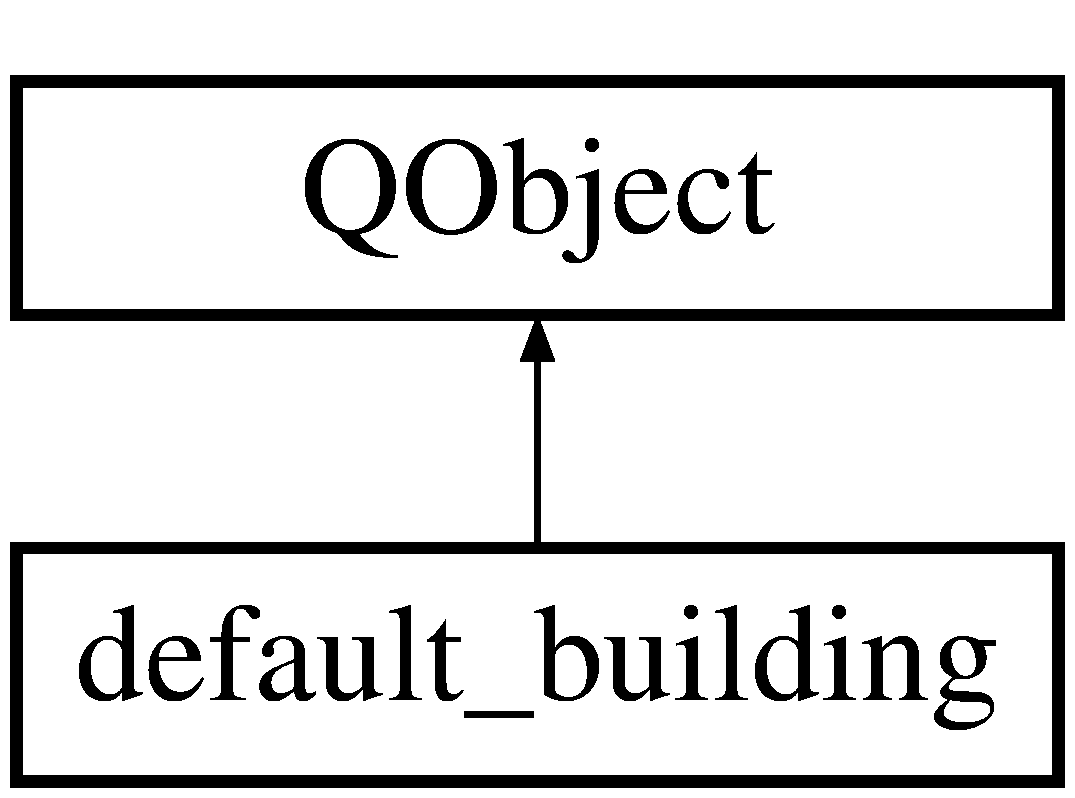
\includegraphics[height=2.000000cm]{classdefault__building}
\end{center}
\end{figure}
\subsection*{Public Member Functions}
\begin{DoxyCompactItemize}
\item 
\hyperlink{classdefault__building_aa00a39e3aec1b2ea8cda18401df560c4}{default\-\_\-building} ()
\begin{DoxyCompactList}\small\item\em Test setup. \end{DoxyCompactList}\end{DoxyCompactItemize}
\subsection*{Private Slots}
\begin{DoxyCompactItemize}
\item 
void \hyperlink{classdefault__building_a6012517a2cdabf2eafc45fe58c1c00c8}{test\-\_\-can\-Be\-Placed\-On\-Tile\-\_\-same\-\_\-owner} ()
\begin{DoxyCompactList}\small\item\em Tests whether an object with the same owner \par
 can be placed on a tile. \end{DoxyCompactList}\item 
void \hyperlink{classdefault__building_ae581115cf5ef510cd11c9ca627cc2520}{test\-\_\-can\-Be\-Placed\-On\-Tile\-\_\-ownerconflict} ()
\begin{DoxyCompactList}\small\item\em Tests whether an object with a different owner \par
 can be placed on a tile. \end{DoxyCompactList}\item 
void \hyperlink{classdefault__building_a1ec8a3bb7a692d66acf8d0b75cd3ba44}{test\-\_\-can\-Be\-Placed\-On\-Tile\-\_\-no\-\_\-owner\-\_\-for\-\_\-tile} ()
\begin{DoxyCompactList}\small\item\em Tests whether an owned object \par
 can be placed on a tile with no owner. \end{DoxyCompactList}\item 
void \hyperlink{classdefault__building_aa27f2bdc2cf8f1c1af513638c6ad392b}{test\-\_\-can\-Be\-Placed\-On\-Tile\-\_\-no\-\_\-owner\-\_\-for\-\_\-object} ()
\begin{DoxyCompactList}\small\item\em Tests whether an object with no owner \par
 can be placed on a tile with an owner. \end{DoxyCompactList}\item 
void \hyperlink{classdefault__building_a949f126050554047ff7e3192e1af3d75}{test\-\_\-can\-Be\-Placed\-On\-Tile\-\_\-no\-\_\-owners} ()
\begin{DoxyCompactList}\small\item\em Tests whether an object with no owner \par
 can be placed on a tile without an owner. \end{DoxyCompactList}\item 
void \hyperlink{classdefault__building_a245adf65bac29aacae6c9f148796157d}{test\-\_\-set\-Location\-Tile} ()
\begin{DoxyCompactList}\small\item\em Tests whether an object can be placed on a tile. \end{DoxyCompactList}\item 
void \hyperlink{classdefault__building_aa20f013a8a7b29bd639f822dd0ec1c2f}{test\-\_\-unset\-Location\-Tile} ()
\begin{DoxyCompactList}\small\item\em Tests whether an object's location can be removed. \end{DoxyCompactList}\item 
void \hyperlink{classdefault__building_a77f6f2948dcbdeda1c89344b4329750e}{test\-\_\-set\-Location\-Tile\-\_\-exception} ()
\begin{DoxyCompactList}\small\item\em Tests whether an object's location can set to a tile \par
with a different owner. \end{DoxyCompactList}\item 
void \hyperlink{classdefault__building_a32db5769634d9638af97d559d6d8aeae}{test\-\_\-current\-Location\-Tile\-\_\-expired\-\_\-ptr} ()
\begin{DoxyCompactList}\small\item\em Tests whether an objects location gets removed if the \par
tile expires it was located on. \end{DoxyCompactList}\item 
void \hyperlink{classdefault__building_a5f5b01449c756e96a14dc7c18e9c778b}{test\-\_\-on\-Build\-Action} ()
\begin{DoxyCompactList}\small\item\em Tests if an H\-Q buildings onbuildaction works. \end{DoxyCompactList}\item 
void \hyperlink{classdefault__building_ace547d46c2ba480530c50e19fcdf99f9}{test\-\_\-add\-Hold\-Markers} ()
\begin{DoxyCompactList}\small\item\em Tests adding a hold marker to a building. \end{DoxyCompactList}\item 
void \hyperlink{classdefault__building_a37386998dea658666fdd3b271ea12262}{test\-\_\-type\-\_\-\-Building\-Base} ()
\begin{DoxyCompactList}\small\item\em Tests Building\-Base's type. \end{DoxyCompactList}\item 
void \hyperlink{classdefault__building_a61e0dccb6b2d2f6caa6d5cb9d6f46761}{test\-\_\-type\-\_\-\-H\-Q} ()
\begin{DoxyCompactList}\small\item\em Tests Head\-Quarter's type. \end{DoxyCompactList}\item 
void \hyperlink{classdefault__building_afb2454e44d8d42562191c5c4cd81b6f7}{test\-\_\-type\-\_\-\-Outpost} ()
\begin{DoxyCompactList}\small\item\em Tests Outpost's type. \end{DoxyCompactList}\item 
void \hyperlink{classdefault__building_a024dda6691de09c78cd2c41c3b2517bb}{test\-\_\-type\-\_\-\-Farm} ()
\begin{DoxyCompactList}\small\item\em Tests Farm's type. \end{DoxyCompactList}\item 
void \hyperlink{classdefault__building_a2629b8493420e49f7d1bffc7c1f085fb}{test\-\_\-type\-\_\-\-Saw\-Mill} ()
\begin{DoxyCompactList}\small\item\em Tests Sawmill's type. \end{DoxyCompactList}\item 
void \hyperlink{classdefault__building_ab331bdbdb301645ece2f9942e5d0b1f4}{test\-\_\-type\-\_\-\-Mine} ()
\begin{DoxyCompactList}\small\item\em Tests Mine's type. \end{DoxyCompactList}\item 
void \hyperlink{classdefault__building_a35e2d98e0d70dd54f04a338c5cf923ae}{cleanup} ()
\begin{DoxyCompactList}\small\item\em Test cleanup. \end{DoxyCompactList}\end{DoxyCompactItemize}
\subsection*{Private Attributes}
\begin{DoxyCompactItemize}
\item 
std\-::shared\-\_\-ptr$<$ \hyperlink{classGame_1_1ObjectManager}{Object\-Manager} $>$ \hyperlink{classdefault__building_a9f19657073191d1ccfae1537bd1bc574}{obj\-Man}
\item 
std\-::shared\-\_\-ptr$<$ \hyperlink{classGame_1_1GameEventHandler}{Game\-Event\-Handler} $>$ \hyperlink{classdefault__building_a7bf9c55301d5a6027d016bf76cb585ce}{G\-E\-Hand}
\item 
std\-::shared\-\_\-ptr$<$ \hyperlink{classGame_1_1Player}{Player} $>$ \hyperlink{classdefault__building_a0459e600394868e19bb88ababc4e50ae}{player1}
\item 
std\-::shared\-\_\-ptr$<$ \hyperlink{classGame_1_1Player}{Player} $>$ \hyperlink{classdefault__building_a27f3d517ae073d9088c533a83a287ba5}{player2}
\item 
std\-::shared\-\_\-ptr$<$ \hyperlink{classCourse_1_1TileBase}{Course\-::\-Tile\-Base} $>$ \hyperlink{classdefault__building_a4851bd1b8736d29d5608dcbd85bca338}{tile1}
\item 
std\-::shared\-\_\-ptr$<$ \hyperlink{classCourse_1_1TileBase}{Course\-::\-Tile\-Base} $>$ \hyperlink{classdefault__building_adcb7e13de2a868910460f1ca658e44b0}{tile2}
\item 
std\-::shared\-\_\-ptr$<$ \hyperlink{classCourse_1_1TileBase}{Course\-::\-Tile\-Base} $>$ \hyperlink{classdefault__building_a03bf0e5b69cdc4c06be2d1ef255f8550}{tile\-Expire}
\item 
const \hyperlink{classCourse_1_1Coordinate}{Course\-::\-Coordinate} \hyperlink{classdefault__building_a9bf0749a6f397a82c5a939fb6fca6f43}{tile1\-\_\-coordinate} = \{1,1\}
\item 
const \hyperlink{classCourse_1_1Coordinate}{Course\-::\-Coordinate} \hyperlink{classdefault__building_a6ba4a9f3044210aacfb738b593a585b7}{tile2\-\_\-coordinate} = \{1,2\}
\item 
const \hyperlink{classCourse_1_1Coordinate}{Course\-::\-Coordinate} \hyperlink{classdefault__building_a5fadd5f10435b00e89e58ce9e32c57e5}{tile\-Expire\-\_\-coordinate} = \{2,2\}
\item 
std\-::shared\-\_\-ptr\\*
$<$ \hyperlink{classCourse_1_1BuildingBase}{Course\-::\-Building\-Base} $>$ \hyperlink{classdefault__building_afa2b3230dc8c603474fcf7dbf76c47c4}{default\-\_\-object}
\item 
std\-::shared\-\_\-ptr\\*
$<$ \hyperlink{classCourse_1_1HeadQuarters}{Course\-::\-Head\-Quarters} $>$ \hyperlink{classdefault__building_a0badf4ed00b36044834272bc3ebf94d3}{hq\-\_\-object}
\item 
std\-::shared\-\_\-ptr$<$ \hyperlink{classCourse_1_1Outpost}{Course\-::\-Outpost} $>$ \hyperlink{classdefault__building_a924c16a0ac49e9b3b9d71d2a27736e93}{outpost\-\_\-object}
\item 
std\-::shared\-\_\-ptr$<$ \hyperlink{classCourse_1_1Farm}{Course\-::\-Farm} $>$ \hyperlink{classdefault__building_aa38e3d845ceeb470e23d4a074f797500}{farm\-\_\-object}
\item 
std\-::shared\-\_\-ptr$<$ \hyperlink{classGame_1_1Mine}{Mine} $>$ \hyperlink{classdefault__building_adceff1efd60baeff9af22c161272c67d}{mine\-\_\-object}
\item 
std\-::shared\-\_\-ptr$<$ \hyperlink{classGame_1_1SawMill}{Saw\-Mill} $>$ \hyperlink{classdefault__building_a17f72da13e6159671242ad6e31ba7fb0}{sawmill\-\_\-object}
\end{DoxyCompactItemize}


\subsection{Detailed Description}
The building\-\_\-tests test the Placeable\-Game\-Object and all Building classes. 

\subsection{Constructor \& Destructor Documentation}
\hypertarget{classdefault__building_aa00a39e3aec1b2ea8cda18401df560c4}{\index{default\-\_\-building@{default\-\_\-building}!default\-\_\-building@{default\-\_\-building}}
\index{default\-\_\-building@{default\-\_\-building}!default_building@{default\-\_\-building}}
\subsubsection[{default\-\_\-building}]{\setlength{\rightskip}{0pt plus 5cm}default\-\_\-building\-::default\-\_\-building (
\begin{DoxyParamCaption}
{}
\end{DoxyParamCaption}
)}}\label{classdefault__building_aa00a39e3aec1b2ea8cda18401df560c4}


Test setup. 



\subsection{Member Function Documentation}
\hypertarget{classdefault__building_a35e2d98e0d70dd54f04a338c5cf923ae}{\index{default\-\_\-building@{default\-\_\-building}!cleanup@{cleanup}}
\index{cleanup@{cleanup}!default_building@{default\-\_\-building}}
\subsubsection[{cleanup}]{\setlength{\rightskip}{0pt plus 5cm}void default\-\_\-building\-::cleanup (
\begin{DoxyParamCaption}
{}
\end{DoxyParamCaption}
)\hspace{0.3cm}{\ttfamily [private]}, {\ttfamily [slot]}}}\label{classdefault__building_a35e2d98e0d70dd54f04a338c5cf923ae}


Test cleanup. 

\hypertarget{classdefault__building_ace547d46c2ba480530c50e19fcdf99f9}{\index{default\-\_\-building@{default\-\_\-building}!test\-\_\-add\-Hold\-Markers@{test\-\_\-add\-Hold\-Markers}}
\index{test\-\_\-add\-Hold\-Markers@{test\-\_\-add\-Hold\-Markers}!default_building@{default\-\_\-building}}
\subsubsection[{test\-\_\-add\-Hold\-Markers}]{\setlength{\rightskip}{0pt plus 5cm}void default\-\_\-building\-::test\-\_\-add\-Hold\-Markers (
\begin{DoxyParamCaption}
{}
\end{DoxyParamCaption}
)\hspace{0.3cm}{\ttfamily [private]}, {\ttfamily [slot]}}}\label{classdefault__building_ace547d46c2ba480530c50e19fcdf99f9}


Tests adding a hold marker to a building. 

\begin{DoxyPostcond}{Postcondition}
Should be possible 
\end{DoxyPostcond}
\hypertarget{classdefault__building_aa27f2bdc2cf8f1c1af513638c6ad392b}{\index{default\-\_\-building@{default\-\_\-building}!test\-\_\-can\-Be\-Placed\-On\-Tile\-\_\-no\-\_\-owner\-\_\-for\-\_\-object@{test\-\_\-can\-Be\-Placed\-On\-Tile\-\_\-no\-\_\-owner\-\_\-for\-\_\-object}}
\index{test\-\_\-can\-Be\-Placed\-On\-Tile\-\_\-no\-\_\-owner\-\_\-for\-\_\-object@{test\-\_\-can\-Be\-Placed\-On\-Tile\-\_\-no\-\_\-owner\-\_\-for\-\_\-object}!default_building@{default\-\_\-building}}
\subsubsection[{test\-\_\-can\-Be\-Placed\-On\-Tile\-\_\-no\-\_\-owner\-\_\-for\-\_\-object}]{\setlength{\rightskip}{0pt plus 5cm}void default\-\_\-building\-::test\-\_\-can\-Be\-Placed\-On\-Tile\-\_\-no\-\_\-owner\-\_\-for\-\_\-object (
\begin{DoxyParamCaption}
{}
\end{DoxyParamCaption}
)\hspace{0.3cm}{\ttfamily [private]}, {\ttfamily [slot]}}}\label{classdefault__building_aa27f2bdc2cf8f1c1af513638c6ad392b}


Tests whether an object with no owner \par
 can be placed on a tile with an owner. 

\begin{DoxyPostcond}{Postcondition}
Should be possible 
\end{DoxyPostcond}
\hypertarget{classdefault__building_a1ec8a3bb7a692d66acf8d0b75cd3ba44}{\index{default\-\_\-building@{default\-\_\-building}!test\-\_\-can\-Be\-Placed\-On\-Tile\-\_\-no\-\_\-owner\-\_\-for\-\_\-tile@{test\-\_\-can\-Be\-Placed\-On\-Tile\-\_\-no\-\_\-owner\-\_\-for\-\_\-tile}}
\index{test\-\_\-can\-Be\-Placed\-On\-Tile\-\_\-no\-\_\-owner\-\_\-for\-\_\-tile@{test\-\_\-can\-Be\-Placed\-On\-Tile\-\_\-no\-\_\-owner\-\_\-for\-\_\-tile}!default_building@{default\-\_\-building}}
\subsubsection[{test\-\_\-can\-Be\-Placed\-On\-Tile\-\_\-no\-\_\-owner\-\_\-for\-\_\-tile}]{\setlength{\rightskip}{0pt plus 5cm}void default\-\_\-building\-::test\-\_\-can\-Be\-Placed\-On\-Tile\-\_\-no\-\_\-owner\-\_\-for\-\_\-tile (
\begin{DoxyParamCaption}
{}
\end{DoxyParamCaption}
)\hspace{0.3cm}{\ttfamily [private]}, {\ttfamily [slot]}}}\label{classdefault__building_a1ec8a3bb7a692d66acf8d0b75cd3ba44}


Tests whether an owned object \par
 can be placed on a tile with no owner. 

\begin{DoxyPostcond}{Postcondition}
Should be possible 
\end{DoxyPostcond}
\hypertarget{classdefault__building_a949f126050554047ff7e3192e1af3d75}{\index{default\-\_\-building@{default\-\_\-building}!test\-\_\-can\-Be\-Placed\-On\-Tile\-\_\-no\-\_\-owners@{test\-\_\-can\-Be\-Placed\-On\-Tile\-\_\-no\-\_\-owners}}
\index{test\-\_\-can\-Be\-Placed\-On\-Tile\-\_\-no\-\_\-owners@{test\-\_\-can\-Be\-Placed\-On\-Tile\-\_\-no\-\_\-owners}!default_building@{default\-\_\-building}}
\subsubsection[{test\-\_\-can\-Be\-Placed\-On\-Tile\-\_\-no\-\_\-owners}]{\setlength{\rightskip}{0pt plus 5cm}void default\-\_\-building\-::test\-\_\-can\-Be\-Placed\-On\-Tile\-\_\-no\-\_\-owners (
\begin{DoxyParamCaption}
{}
\end{DoxyParamCaption}
)\hspace{0.3cm}{\ttfamily [private]}, {\ttfamily [slot]}}}\label{classdefault__building_a949f126050554047ff7e3192e1af3d75}


Tests whether an object with no owner \par
 can be placed on a tile without an owner. 

\begin{DoxyPostcond}{Postcondition}
Should be possible 
\end{DoxyPostcond}
\hypertarget{classdefault__building_ae581115cf5ef510cd11c9ca627cc2520}{\index{default\-\_\-building@{default\-\_\-building}!test\-\_\-can\-Be\-Placed\-On\-Tile\-\_\-ownerconflict@{test\-\_\-can\-Be\-Placed\-On\-Tile\-\_\-ownerconflict}}
\index{test\-\_\-can\-Be\-Placed\-On\-Tile\-\_\-ownerconflict@{test\-\_\-can\-Be\-Placed\-On\-Tile\-\_\-ownerconflict}!default_building@{default\-\_\-building}}
\subsubsection[{test\-\_\-can\-Be\-Placed\-On\-Tile\-\_\-ownerconflict}]{\setlength{\rightskip}{0pt plus 5cm}void default\-\_\-building\-::test\-\_\-can\-Be\-Placed\-On\-Tile\-\_\-ownerconflict (
\begin{DoxyParamCaption}
{}
\end{DoxyParamCaption}
)\hspace{0.3cm}{\ttfamily [private]}, {\ttfamily [slot]}}}\label{classdefault__building_ae581115cf5ef510cd11c9ca627cc2520}


Tests whether an object with a different owner \par
 can be placed on a tile. 

\begin{DoxyPostcond}{Postcondition}
Should not be possible 
\end{DoxyPostcond}
\hypertarget{classdefault__building_a6012517a2cdabf2eafc45fe58c1c00c8}{\index{default\-\_\-building@{default\-\_\-building}!test\-\_\-can\-Be\-Placed\-On\-Tile\-\_\-same\-\_\-owner@{test\-\_\-can\-Be\-Placed\-On\-Tile\-\_\-same\-\_\-owner}}
\index{test\-\_\-can\-Be\-Placed\-On\-Tile\-\_\-same\-\_\-owner@{test\-\_\-can\-Be\-Placed\-On\-Tile\-\_\-same\-\_\-owner}!default_building@{default\-\_\-building}}
\subsubsection[{test\-\_\-can\-Be\-Placed\-On\-Tile\-\_\-same\-\_\-owner}]{\setlength{\rightskip}{0pt plus 5cm}void default\-\_\-building\-::test\-\_\-can\-Be\-Placed\-On\-Tile\-\_\-same\-\_\-owner (
\begin{DoxyParamCaption}
{}
\end{DoxyParamCaption}
)\hspace{0.3cm}{\ttfamily [private]}, {\ttfamily [slot]}}}\label{classdefault__building_a6012517a2cdabf2eafc45fe58c1c00c8}


Tests whether an object with the same owner \par
 can be placed on a tile. 

\begin{DoxyPostcond}{Postcondition}
Should be possible 
\end{DoxyPostcond}
\hypertarget{classdefault__building_a32db5769634d9638af97d559d6d8aeae}{\index{default\-\_\-building@{default\-\_\-building}!test\-\_\-current\-Location\-Tile\-\_\-expired\-\_\-ptr@{test\-\_\-current\-Location\-Tile\-\_\-expired\-\_\-ptr}}
\index{test\-\_\-current\-Location\-Tile\-\_\-expired\-\_\-ptr@{test\-\_\-current\-Location\-Tile\-\_\-expired\-\_\-ptr}!default_building@{default\-\_\-building}}
\subsubsection[{test\-\_\-current\-Location\-Tile\-\_\-expired\-\_\-ptr}]{\setlength{\rightskip}{0pt plus 5cm}void default\-\_\-building\-::test\-\_\-current\-Location\-Tile\-\_\-expired\-\_\-ptr (
\begin{DoxyParamCaption}
{}
\end{DoxyParamCaption}
)\hspace{0.3cm}{\ttfamily [private]}, {\ttfamily [slot]}}}\label{classdefault__building_a32db5769634d9638af97d559d6d8aeae}


Tests whether an objects location gets removed if the \par
tile expires it was located on. 

\begin{DoxyPostcond}{Postcondition}
Should be removed 
\end{DoxyPostcond}
\hypertarget{classdefault__building_a5f5b01449c756e96a14dc7c18e9c778b}{\index{default\-\_\-building@{default\-\_\-building}!test\-\_\-on\-Build\-Action@{test\-\_\-on\-Build\-Action}}
\index{test\-\_\-on\-Build\-Action@{test\-\_\-on\-Build\-Action}!default_building@{default\-\_\-building}}
\subsubsection[{test\-\_\-on\-Build\-Action}]{\setlength{\rightskip}{0pt plus 5cm}void default\-\_\-building\-::test\-\_\-on\-Build\-Action (
\begin{DoxyParamCaption}
{}
\end{DoxyParamCaption}
)\hspace{0.3cm}{\ttfamily [private]}, {\ttfamily [slot]}}}\label{classdefault__building_a5f5b01449c756e96a14dc7c18e9c778b}


Tests if an H\-Q buildings onbuildaction works. 

\begin{DoxyPostcond}{Postcondition}
Should work 
\end{DoxyPostcond}
\hypertarget{classdefault__building_a245adf65bac29aacae6c9f148796157d}{\index{default\-\_\-building@{default\-\_\-building}!test\-\_\-set\-Location\-Tile@{test\-\_\-set\-Location\-Tile}}
\index{test\-\_\-set\-Location\-Tile@{test\-\_\-set\-Location\-Tile}!default_building@{default\-\_\-building}}
\subsubsection[{test\-\_\-set\-Location\-Tile}]{\setlength{\rightskip}{0pt plus 5cm}void default\-\_\-building\-::test\-\_\-set\-Location\-Tile (
\begin{DoxyParamCaption}
{}
\end{DoxyParamCaption}
)\hspace{0.3cm}{\ttfamily [private]}, {\ttfamily [slot]}}}\label{classdefault__building_a245adf65bac29aacae6c9f148796157d}


Tests whether an object can be placed on a tile. 

\begin{DoxyPostcond}{Postcondition}
Should be possible 
\end{DoxyPostcond}
\hypertarget{classdefault__building_a77f6f2948dcbdeda1c89344b4329750e}{\index{default\-\_\-building@{default\-\_\-building}!test\-\_\-set\-Location\-Tile\-\_\-exception@{test\-\_\-set\-Location\-Tile\-\_\-exception}}
\index{test\-\_\-set\-Location\-Tile\-\_\-exception@{test\-\_\-set\-Location\-Tile\-\_\-exception}!default_building@{default\-\_\-building}}
\subsubsection[{test\-\_\-set\-Location\-Tile\-\_\-exception}]{\setlength{\rightskip}{0pt plus 5cm}void default\-\_\-building\-::test\-\_\-set\-Location\-Tile\-\_\-exception (
\begin{DoxyParamCaption}
{}
\end{DoxyParamCaption}
)\hspace{0.3cm}{\ttfamily [private]}, {\ttfamily [slot]}}}\label{classdefault__building_a77f6f2948dcbdeda1c89344b4329750e}


Tests whether an object's location can set to a tile \par
with a different owner. 

\begin{DoxyPostcond}{Postcondition}
Should throw an Illegal\-Action exception 
\end{DoxyPostcond}
\hypertarget{classdefault__building_a37386998dea658666fdd3b271ea12262}{\index{default\-\_\-building@{default\-\_\-building}!test\-\_\-type\-\_\-\-Building\-Base@{test\-\_\-type\-\_\-\-Building\-Base}}
\index{test\-\_\-type\-\_\-\-Building\-Base@{test\-\_\-type\-\_\-\-Building\-Base}!default_building@{default\-\_\-building}}
\subsubsection[{test\-\_\-type\-\_\-\-Building\-Base}]{\setlength{\rightskip}{0pt plus 5cm}void default\-\_\-building\-::test\-\_\-type\-\_\-\-Building\-Base (
\begin{DoxyParamCaption}
{}
\end{DoxyParamCaption}
)\hspace{0.3cm}{\ttfamily [private]}, {\ttfamily [slot]}}}\label{classdefault__building_a37386998dea658666fdd3b271ea12262}


Tests Building\-Base's type. 

\begin{DoxyPostcond}{Postcondition}
Should be Building\-Base 
\end{DoxyPostcond}
\hypertarget{classdefault__building_a024dda6691de09c78cd2c41c3b2517bb}{\index{default\-\_\-building@{default\-\_\-building}!test\-\_\-type\-\_\-\-Farm@{test\-\_\-type\-\_\-\-Farm}}
\index{test\-\_\-type\-\_\-\-Farm@{test\-\_\-type\-\_\-\-Farm}!default_building@{default\-\_\-building}}
\subsubsection[{test\-\_\-type\-\_\-\-Farm}]{\setlength{\rightskip}{0pt plus 5cm}void default\-\_\-building\-::test\-\_\-type\-\_\-\-Farm (
\begin{DoxyParamCaption}
{}
\end{DoxyParamCaption}
)\hspace{0.3cm}{\ttfamily [private]}, {\ttfamily [slot]}}}\label{classdefault__building_a024dda6691de09c78cd2c41c3b2517bb}


Tests Farm's type. 

\begin{DoxyPostcond}{Postcondition}
Should be Farm 
\end{DoxyPostcond}
\hypertarget{classdefault__building_a61e0dccb6b2d2f6caa6d5cb9d6f46761}{\index{default\-\_\-building@{default\-\_\-building}!test\-\_\-type\-\_\-\-H\-Q@{test\-\_\-type\-\_\-\-H\-Q}}
\index{test\-\_\-type\-\_\-\-H\-Q@{test\-\_\-type\-\_\-\-H\-Q}!default_building@{default\-\_\-building}}
\subsubsection[{test\-\_\-type\-\_\-\-H\-Q}]{\setlength{\rightskip}{0pt plus 5cm}void default\-\_\-building\-::test\-\_\-type\-\_\-\-H\-Q (
\begin{DoxyParamCaption}
{}
\end{DoxyParamCaption}
)\hspace{0.3cm}{\ttfamily [private]}, {\ttfamily [slot]}}}\label{classdefault__building_a61e0dccb6b2d2f6caa6d5cb9d6f46761}


Tests Head\-Quarter's type. 

\begin{DoxyPostcond}{Postcondition}
Should be Head\-Quarters 
\end{DoxyPostcond}
\hypertarget{classdefault__building_ab331bdbdb301645ece2f9942e5d0b1f4}{\index{default\-\_\-building@{default\-\_\-building}!test\-\_\-type\-\_\-\-Mine@{test\-\_\-type\-\_\-\-Mine}}
\index{test\-\_\-type\-\_\-\-Mine@{test\-\_\-type\-\_\-\-Mine}!default_building@{default\-\_\-building}}
\subsubsection[{test\-\_\-type\-\_\-\-Mine}]{\setlength{\rightskip}{0pt plus 5cm}void default\-\_\-building\-::test\-\_\-type\-\_\-\-Mine (
\begin{DoxyParamCaption}
{}
\end{DoxyParamCaption}
)\hspace{0.3cm}{\ttfamily [private]}, {\ttfamily [slot]}}}\label{classdefault__building_ab331bdbdb301645ece2f9942e5d0b1f4}


Tests Mine's type. 

\begin{DoxyPostcond}{Postcondition}
Should be Mine 
\end{DoxyPostcond}
\hypertarget{classdefault__building_afb2454e44d8d42562191c5c4cd81b6f7}{\index{default\-\_\-building@{default\-\_\-building}!test\-\_\-type\-\_\-\-Outpost@{test\-\_\-type\-\_\-\-Outpost}}
\index{test\-\_\-type\-\_\-\-Outpost@{test\-\_\-type\-\_\-\-Outpost}!default_building@{default\-\_\-building}}
\subsubsection[{test\-\_\-type\-\_\-\-Outpost}]{\setlength{\rightskip}{0pt plus 5cm}void default\-\_\-building\-::test\-\_\-type\-\_\-\-Outpost (
\begin{DoxyParamCaption}
{}
\end{DoxyParamCaption}
)\hspace{0.3cm}{\ttfamily [private]}, {\ttfamily [slot]}}}\label{classdefault__building_afb2454e44d8d42562191c5c4cd81b6f7}


Tests Outpost's type. 

\begin{DoxyPostcond}{Postcondition}
Should be Outpost 
\end{DoxyPostcond}
\hypertarget{classdefault__building_a2629b8493420e49f7d1bffc7c1f085fb}{\index{default\-\_\-building@{default\-\_\-building}!test\-\_\-type\-\_\-\-Saw\-Mill@{test\-\_\-type\-\_\-\-Saw\-Mill}}
\index{test\-\_\-type\-\_\-\-Saw\-Mill@{test\-\_\-type\-\_\-\-Saw\-Mill}!default_building@{default\-\_\-building}}
\subsubsection[{test\-\_\-type\-\_\-\-Saw\-Mill}]{\setlength{\rightskip}{0pt plus 5cm}void default\-\_\-building\-::test\-\_\-type\-\_\-\-Saw\-Mill (
\begin{DoxyParamCaption}
{}
\end{DoxyParamCaption}
)\hspace{0.3cm}{\ttfamily [private]}, {\ttfamily [slot]}}}\label{classdefault__building_a2629b8493420e49f7d1bffc7c1f085fb}


Tests Sawmill's type. 

\begin{DoxyPostcond}{Postcondition}
Should be Sawmill 
\end{DoxyPostcond}
\hypertarget{classdefault__building_aa20f013a8a7b29bd639f822dd0ec1c2f}{\index{default\-\_\-building@{default\-\_\-building}!test\-\_\-unset\-Location\-Tile@{test\-\_\-unset\-Location\-Tile}}
\index{test\-\_\-unset\-Location\-Tile@{test\-\_\-unset\-Location\-Tile}!default_building@{default\-\_\-building}}
\subsubsection[{test\-\_\-unset\-Location\-Tile}]{\setlength{\rightskip}{0pt plus 5cm}void default\-\_\-building\-::test\-\_\-unset\-Location\-Tile (
\begin{DoxyParamCaption}
{}
\end{DoxyParamCaption}
)\hspace{0.3cm}{\ttfamily [private]}, {\ttfamily [slot]}}}\label{classdefault__building_aa20f013a8a7b29bd639f822dd0ec1c2f}


Tests whether an object's location can be removed. 

\begin{DoxyPostcond}{Postcondition}
Should be possible 
\end{DoxyPostcond}


\subsection{Member Data Documentation}
\hypertarget{classdefault__building_afa2b3230dc8c603474fcf7dbf76c47c4}{\index{default\-\_\-building@{default\-\_\-building}!default\-\_\-object@{default\-\_\-object}}
\index{default\-\_\-object@{default\-\_\-object}!default_building@{default\-\_\-building}}
\subsubsection[{default\-\_\-object}]{\setlength{\rightskip}{0pt plus 5cm}std\-::shared\-\_\-ptr$<${\bf Course\-::\-Building\-Base}$>$ default\-\_\-building\-::default\-\_\-object\hspace{0.3cm}{\ttfamily [private]}}}\label{classdefault__building_afa2b3230dc8c603474fcf7dbf76c47c4}
\hypertarget{classdefault__building_aa38e3d845ceeb470e23d4a074f797500}{\index{default\-\_\-building@{default\-\_\-building}!farm\-\_\-object@{farm\-\_\-object}}
\index{farm\-\_\-object@{farm\-\_\-object}!default_building@{default\-\_\-building}}
\subsubsection[{farm\-\_\-object}]{\setlength{\rightskip}{0pt plus 5cm}std\-::shared\-\_\-ptr$<${\bf Course\-::\-Farm}$>$ default\-\_\-building\-::farm\-\_\-object\hspace{0.3cm}{\ttfamily [private]}}}\label{classdefault__building_aa38e3d845ceeb470e23d4a074f797500}
\hypertarget{classdefault__building_a7bf9c55301d5a6027d016bf76cb585ce}{\index{default\-\_\-building@{default\-\_\-building}!G\-E\-Hand@{G\-E\-Hand}}
\index{G\-E\-Hand@{G\-E\-Hand}!default_building@{default\-\_\-building}}
\subsubsection[{G\-E\-Hand}]{\setlength{\rightskip}{0pt plus 5cm}std\-::shared\-\_\-ptr$<${\bf Game\-Event\-Handler}$>$ default\-\_\-building\-::\-G\-E\-Hand\hspace{0.3cm}{\ttfamily [private]}}}\label{classdefault__building_a7bf9c55301d5a6027d016bf76cb585ce}
\hypertarget{classdefault__building_a0badf4ed00b36044834272bc3ebf94d3}{\index{default\-\_\-building@{default\-\_\-building}!hq\-\_\-object@{hq\-\_\-object}}
\index{hq\-\_\-object@{hq\-\_\-object}!default_building@{default\-\_\-building}}
\subsubsection[{hq\-\_\-object}]{\setlength{\rightskip}{0pt plus 5cm}std\-::shared\-\_\-ptr$<${\bf Course\-::\-Head\-Quarters}$>$ default\-\_\-building\-::hq\-\_\-object\hspace{0.3cm}{\ttfamily [private]}}}\label{classdefault__building_a0badf4ed00b36044834272bc3ebf94d3}
\hypertarget{classdefault__building_adceff1efd60baeff9af22c161272c67d}{\index{default\-\_\-building@{default\-\_\-building}!mine\-\_\-object@{mine\-\_\-object}}
\index{mine\-\_\-object@{mine\-\_\-object}!default_building@{default\-\_\-building}}
\subsubsection[{mine\-\_\-object}]{\setlength{\rightskip}{0pt plus 5cm}std\-::shared\-\_\-ptr$<${\bf Mine}$>$ default\-\_\-building\-::mine\-\_\-object\hspace{0.3cm}{\ttfamily [private]}}}\label{classdefault__building_adceff1efd60baeff9af22c161272c67d}
\hypertarget{classdefault__building_a9f19657073191d1ccfae1537bd1bc574}{\index{default\-\_\-building@{default\-\_\-building}!obj\-Man@{obj\-Man}}
\index{obj\-Man@{obj\-Man}!default_building@{default\-\_\-building}}
\subsubsection[{obj\-Man}]{\setlength{\rightskip}{0pt plus 5cm}std\-::shared\-\_\-ptr$<${\bf Object\-Manager}$>$ default\-\_\-building\-::obj\-Man\hspace{0.3cm}{\ttfamily [private]}}}\label{classdefault__building_a9f19657073191d1ccfae1537bd1bc574}
\hypertarget{classdefault__building_a924c16a0ac49e9b3b9d71d2a27736e93}{\index{default\-\_\-building@{default\-\_\-building}!outpost\-\_\-object@{outpost\-\_\-object}}
\index{outpost\-\_\-object@{outpost\-\_\-object}!default_building@{default\-\_\-building}}
\subsubsection[{outpost\-\_\-object}]{\setlength{\rightskip}{0pt plus 5cm}std\-::shared\-\_\-ptr$<${\bf Course\-::\-Outpost}$>$ default\-\_\-building\-::outpost\-\_\-object\hspace{0.3cm}{\ttfamily [private]}}}\label{classdefault__building_a924c16a0ac49e9b3b9d71d2a27736e93}
\hypertarget{classdefault__building_a0459e600394868e19bb88ababc4e50ae}{\index{default\-\_\-building@{default\-\_\-building}!player1@{player1}}
\index{player1@{player1}!default_building@{default\-\_\-building}}
\subsubsection[{player1}]{\setlength{\rightskip}{0pt plus 5cm}std\-::shared\-\_\-ptr$<${\bf Player}$>$ default\-\_\-building\-::player1\hspace{0.3cm}{\ttfamily [private]}}}\label{classdefault__building_a0459e600394868e19bb88ababc4e50ae}
\hypertarget{classdefault__building_a27f3d517ae073d9088c533a83a287ba5}{\index{default\-\_\-building@{default\-\_\-building}!player2@{player2}}
\index{player2@{player2}!default_building@{default\-\_\-building}}
\subsubsection[{player2}]{\setlength{\rightskip}{0pt plus 5cm}std\-::shared\-\_\-ptr$<${\bf Player}$>$ default\-\_\-building\-::player2\hspace{0.3cm}{\ttfamily [private]}}}\label{classdefault__building_a27f3d517ae073d9088c533a83a287ba5}
\hypertarget{classdefault__building_a17f72da13e6159671242ad6e31ba7fb0}{\index{default\-\_\-building@{default\-\_\-building}!sawmill\-\_\-object@{sawmill\-\_\-object}}
\index{sawmill\-\_\-object@{sawmill\-\_\-object}!default_building@{default\-\_\-building}}
\subsubsection[{sawmill\-\_\-object}]{\setlength{\rightskip}{0pt plus 5cm}std\-::shared\-\_\-ptr$<${\bf Saw\-Mill}$>$ default\-\_\-building\-::sawmill\-\_\-object\hspace{0.3cm}{\ttfamily [private]}}}\label{classdefault__building_a17f72da13e6159671242ad6e31ba7fb0}
\hypertarget{classdefault__building_a4851bd1b8736d29d5608dcbd85bca338}{\index{default\-\_\-building@{default\-\_\-building}!tile1@{tile1}}
\index{tile1@{tile1}!default_building@{default\-\_\-building}}
\subsubsection[{tile1}]{\setlength{\rightskip}{0pt plus 5cm}std\-::shared\-\_\-ptr$<${\bf Course\-::\-Tile\-Base}$>$ default\-\_\-building\-::tile1\hspace{0.3cm}{\ttfamily [private]}}}\label{classdefault__building_a4851bd1b8736d29d5608dcbd85bca338}
\hypertarget{classdefault__building_a9bf0749a6f397a82c5a939fb6fca6f43}{\index{default\-\_\-building@{default\-\_\-building}!tile1\-\_\-coordinate@{tile1\-\_\-coordinate}}
\index{tile1\-\_\-coordinate@{tile1\-\_\-coordinate}!default_building@{default\-\_\-building}}
\subsubsection[{tile1\-\_\-coordinate}]{\setlength{\rightskip}{0pt plus 5cm}const {\bf Course\-::\-Coordinate} default\-\_\-building\-::tile1\-\_\-coordinate = \{1,1\}\hspace{0.3cm}{\ttfamily [private]}}}\label{classdefault__building_a9bf0749a6f397a82c5a939fb6fca6f43}
\hypertarget{classdefault__building_adcb7e13de2a868910460f1ca658e44b0}{\index{default\-\_\-building@{default\-\_\-building}!tile2@{tile2}}
\index{tile2@{tile2}!default_building@{default\-\_\-building}}
\subsubsection[{tile2}]{\setlength{\rightskip}{0pt plus 5cm}std\-::shared\-\_\-ptr$<${\bf Course\-::\-Tile\-Base}$>$ default\-\_\-building\-::tile2\hspace{0.3cm}{\ttfamily [private]}}}\label{classdefault__building_adcb7e13de2a868910460f1ca658e44b0}
\hypertarget{classdefault__building_a6ba4a9f3044210aacfb738b593a585b7}{\index{default\-\_\-building@{default\-\_\-building}!tile2\-\_\-coordinate@{tile2\-\_\-coordinate}}
\index{tile2\-\_\-coordinate@{tile2\-\_\-coordinate}!default_building@{default\-\_\-building}}
\subsubsection[{tile2\-\_\-coordinate}]{\setlength{\rightskip}{0pt plus 5cm}const {\bf Course\-::\-Coordinate} default\-\_\-building\-::tile2\-\_\-coordinate = \{1,2\}\hspace{0.3cm}{\ttfamily [private]}}}\label{classdefault__building_a6ba4a9f3044210aacfb738b593a585b7}
\hypertarget{classdefault__building_a03bf0e5b69cdc4c06be2d1ef255f8550}{\index{default\-\_\-building@{default\-\_\-building}!tile\-Expire@{tile\-Expire}}
\index{tile\-Expire@{tile\-Expire}!default_building@{default\-\_\-building}}
\subsubsection[{tile\-Expire}]{\setlength{\rightskip}{0pt plus 5cm}std\-::shared\-\_\-ptr$<${\bf Course\-::\-Tile\-Base}$>$ default\-\_\-building\-::tile\-Expire\hspace{0.3cm}{\ttfamily [private]}}}\label{classdefault__building_a03bf0e5b69cdc4c06be2d1ef255f8550}
\hypertarget{classdefault__building_a5fadd5f10435b00e89e58ce9e32c57e5}{\index{default\-\_\-building@{default\-\_\-building}!tile\-Expire\-\_\-coordinate@{tile\-Expire\-\_\-coordinate}}
\index{tile\-Expire\-\_\-coordinate@{tile\-Expire\-\_\-coordinate}!default_building@{default\-\_\-building}}
\subsubsection[{tile\-Expire\-\_\-coordinate}]{\setlength{\rightskip}{0pt plus 5cm}const {\bf Course\-::\-Coordinate} default\-\_\-building\-::tile\-Expire\-\_\-coordinate = \{2,2\}\hspace{0.3cm}{\ttfamily [private]}}}\label{classdefault__building_a5fadd5f10435b00e89e58ce9e32c57e5}


The documentation for this class was generated from the following file\-:\begin{DoxyCompactItemize}
\item 
Unit\-Tests/building\-\_\-tests/\hyperlink{tst__default__building_8cpp}{tst\-\_\-default\-\_\-building.\-cpp}\end{DoxyCompactItemize}

\hypertarget{classdefault__coordinate}{\section{default\-\_\-coordinate Class Reference}
\label{classdefault__coordinate}\index{default\-\_\-coordinate@{default\-\_\-coordinate}}
}
Inheritance diagram for default\-\_\-coordinate\-:\begin{figure}[H]
\begin{center}
\leavevmode
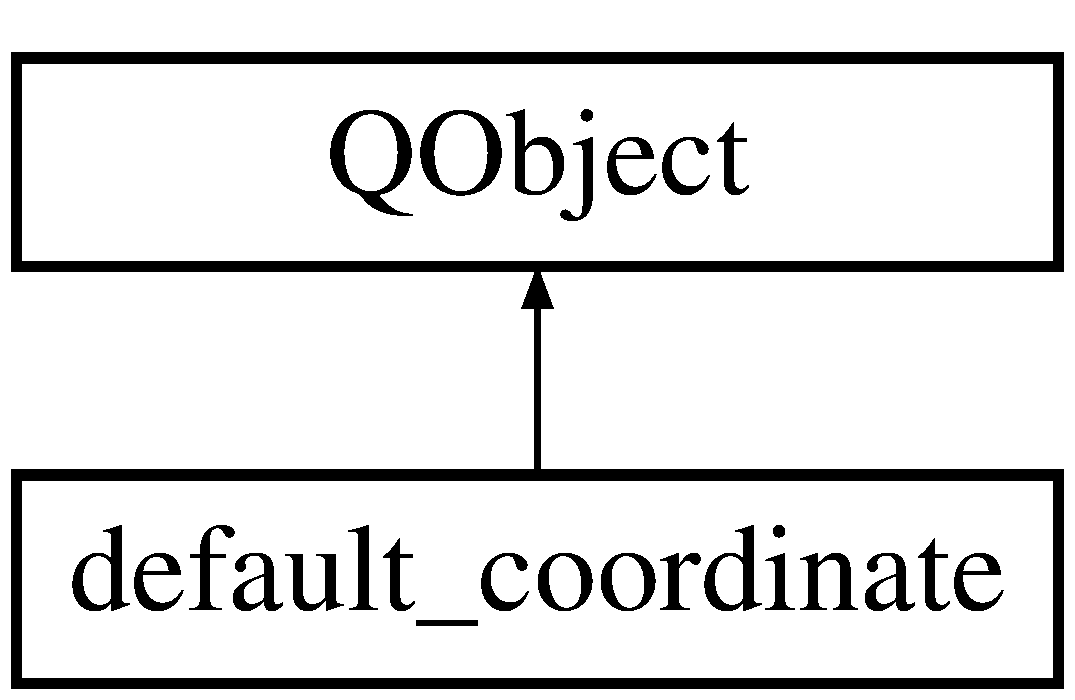
\includegraphics[height=2.000000cm]{classdefault__coordinate}
\end{center}
\end{figure}
\subsection*{Public Member Functions}
\begin{DoxyCompactItemize}
\item 
\hyperlink{classdefault__coordinate_a34568bfc14507a9621db3d8c3a7d689c}{default\-\_\-coordinate} ()
\item 
\hyperlink{classdefault__coordinate_a574a76c27abca08cb68d259024350b48}{$\sim$default\-\_\-coordinate} ()
\end{DoxyCompactItemize}
\subsection*{Private Slots}
\begin{DoxyCompactItemize}
\item 
void \hyperlink{classdefault__coordinate_a71fcd0aa8e050299b51d37d0a5510693}{test\-\_\-copy\-\_\-constructor} ()
\item 
void \hyperlink{classdefault__coordinate_ab509ca94677873f51fd7f36ff08f6b6e}{test\-\_\-copy\-\_\-constructor\-\_\-with\-\_\-direction} ()
\item 
void \hyperlink{classdefault__coordinate_aea1ecde0e6af8c66f4ae09b859ba9abe}{test\-\_\-copy\-\_\-constructor\-\_\-with\-\_\-direction\-\_\-data} ()
\item 
void \hyperlink{classdefault__coordinate_a6ac1346bb3e21f989282554eeff6fa6b}{test\-\_\-copy\-\_\-constructor\-\_\-with\-\_\-direction\-\_\-and\-\_\-distance} ()
\item 
void \hyperlink{classdefault__coordinate_a8c8c4df572230ebc9421ab39cfb236cb}{test\-\_\-copy\-\_\-constructor\-\_\-with\-\_\-direction\-\_\-and\-\_\-distance\-\_\-data} ()
\item 
void \hyperlink{classdefault__coordinate_acdd8347e4ae9325221f1056270d1ef5b}{test\-\_\-travel} ()
\item 
void \hyperlink{classdefault__coordinate_a66fb93f53378b5448839a822e9942c98}{test\-\_\-neighbour\-\_\-at} ()
\item 
void \hyperlink{classdefault__coordinate_ae6eaad96449fbbad9058494c33347f19}{test\-\_\-neighbour\-\_\-at\-\_\-data} ()
\item 
void \hyperlink{classdefault__coordinate_a1d8fe20449e7ace996ce4728c932259b}{test\-\_\-neighbours} ()
\item 
void \hyperlink{classdefault__coordinate_acd5ed771bff170097b543bb461c01541}{test\-\_\-neighbours\-\_\-data} ()
\item 
void \hyperlink{classdefault__coordinate_aaa187cf2b16d29002fcb03e9144f3e52}{test\-\_\-operator\-\_\-plus} ()
\item 
void \hyperlink{classdefault__coordinate_a26a03d9d0a1d9c9e4d168c66a9799fa5}{test\-\_\-operator\-\_\-plus\-\_\-data} ()
\item 
void \hyperlink{classdefault__coordinate_a5408954bafdc1ef476508e844cfbc14e}{test\-\_\-operator\-\_\-plus\-\_\-assign} ()
\item 
void \hyperlink{classdefault__coordinate_adfc67ea0828768f5dbdc2ee0c20291a4}{test\-\_\-operator\-\_\-plus\-\_\-assign\-\_\-data} ()
\item 
void \hyperlink{classdefault__coordinate_a2463062e598f41469a914e98b5dc854c}{test\-\_\-operator\-\_\-minus} ()
\item 
void \hyperlink{classdefault__coordinate_a70361e17e1f04ec66e5a69600efbf825}{test\-\_\-operator\-\_\-minus\-\_\-data} ()
\item 
void \hyperlink{classdefault__coordinate_af8a4fdae768857a0f44d4ad4097b4809}{test\-\_\-operator\-\_\-minus\-\_\-assign} ()
\item 
void \hyperlink{classdefault__coordinate_a85986ef5c89e795409c2768de91374ad}{test\-\_\-operator\-\_\-minus\-\_\-assign\-\_\-data} ()
\item 
void \hyperlink{classdefault__coordinate_ab40158075fa6172ecf6d920692d77f07}{test\-\_\-operator\-\_\-assign} ()
\item 
void \hyperlink{classdefault__coordinate_a6782b4cbf116fd532cd24aa124114647}{test\-\_\-comp\-\_\-eq} ()
\item 
void \hyperlink{classdefault__coordinate_a79b6f2cb5036b81ee9065bfb229407a9}{test\-\_\-comp\-\_\-eq\-\_\-data} ()
\item 
void \hyperlink{classdefault__coordinate_a62f69b8f3c4b13d1a19f888a535c1a05}{test\-\_\-comp\-\_\-neq} ()
\item 
void \hyperlink{classdefault__coordinate_a65d7a41b67e6c5075e3f7fef9408fb9e}{test\-\_\-comp\-\_\-neq\-\_\-data} ()
\item 
void \hyperlink{classdefault__coordinate_afc1c3cb28786b5541c43d737f01d6c11}{test\-\_\-comp\-\_\-lt} ()
\item 
void \hyperlink{classdefault__coordinate_a4bdc273fc3d3afc49538b71a9adfab34}{test\-\_\-comp\-\_\-lt\-\_\-data} ()
\item 
void \hyperlink{classdefault__coordinate_ac7aefb8e1de41575fb1575ea2a433c33}{test\-\_\-comp\-\_\-gt} ()
\item 
void \hyperlink{classdefault__coordinate_abed751bd23e0a376c1936619180f65eb}{test\-\_\-comp\-\_\-gt\-\_\-data} ()
\item 
void \hyperlink{classdefault__coordinate_a26c8d9d10a130b4a0e38dfede89b8f78}{test\-\_\-comp\-\_\-elt} ()
\item 
void \hyperlink{classdefault__coordinate_a5d1b77894f89c13449f4adeff5dd672c}{test\-\_\-comp\-\_\-elt\-\_\-data} ()
\item 
void \hyperlink{classdefault__coordinate_a3e141673c8500ca0a12c8bfb5a94b3e9}{test\-\_\-comp\-\_\-egt} ()
\item 
void \hyperlink{classdefault__coordinate_af0c0b6109339ba69c910fde934b0a301}{test\-\_\-comp\-\_\-egt\-\_\-data} ()
\end{DoxyCompactItemize}
\subsection*{Private Attributes}
\begin{DoxyCompactItemize}
\item 
const \hyperlink{classCourse_1_1Coordinate}{Coordinate} \hyperlink{classdefault__coordinate_a817a4c307ee99f7b58176370eda227e8}{O\-R\-I\-G\-I\-N} = \hyperlink{classCourse_1_1Coordinate}{Coordinate}(0,0)
\end{DoxyCompactItemize}


\subsection{Constructor \& Destructor Documentation}
\hypertarget{classdefault__coordinate_a34568bfc14507a9621db3d8c3a7d689c}{\index{default\-\_\-coordinate@{default\-\_\-coordinate}!default\-\_\-coordinate@{default\-\_\-coordinate}}
\index{default\-\_\-coordinate@{default\-\_\-coordinate}!default_coordinate@{default\-\_\-coordinate}}
\subsubsection[{default\-\_\-coordinate}]{\setlength{\rightskip}{0pt plus 5cm}default\-\_\-coordinate\-::default\-\_\-coordinate (
\begin{DoxyParamCaption}
{}
\end{DoxyParamCaption}
)}}\label{classdefault__coordinate_a34568bfc14507a9621db3d8c3a7d689c}
\hypertarget{classdefault__coordinate_a574a76c27abca08cb68d259024350b48}{\index{default\-\_\-coordinate@{default\-\_\-coordinate}!$\sim$default\-\_\-coordinate@{$\sim$default\-\_\-coordinate}}
\index{$\sim$default\-\_\-coordinate@{$\sim$default\-\_\-coordinate}!default_coordinate@{default\-\_\-coordinate}}
\subsubsection[{$\sim$default\-\_\-coordinate}]{\setlength{\rightskip}{0pt plus 5cm}default\-\_\-coordinate\-::$\sim$default\-\_\-coordinate (
\begin{DoxyParamCaption}
{}
\end{DoxyParamCaption}
)}}\label{classdefault__coordinate_a574a76c27abca08cb68d259024350b48}


\subsection{Member Function Documentation}
\hypertarget{classdefault__coordinate_a3e141673c8500ca0a12c8bfb5a94b3e9}{\index{default\-\_\-coordinate@{default\-\_\-coordinate}!test\-\_\-comp\-\_\-egt@{test\-\_\-comp\-\_\-egt}}
\index{test\-\_\-comp\-\_\-egt@{test\-\_\-comp\-\_\-egt}!default_coordinate@{default\-\_\-coordinate}}
\subsubsection[{test\-\_\-comp\-\_\-egt}]{\setlength{\rightskip}{0pt plus 5cm}void default\-\_\-coordinate\-::test\-\_\-comp\-\_\-egt (
\begin{DoxyParamCaption}
{}
\end{DoxyParamCaption}
)\hspace{0.3cm}{\ttfamily [private]}, {\ttfamily [slot]}}}\label{classdefault__coordinate_a3e141673c8500ca0a12c8bfb5a94b3e9}
\hypertarget{classdefault__coordinate_af0c0b6109339ba69c910fde934b0a301}{\index{default\-\_\-coordinate@{default\-\_\-coordinate}!test\-\_\-comp\-\_\-egt\-\_\-data@{test\-\_\-comp\-\_\-egt\-\_\-data}}
\index{test\-\_\-comp\-\_\-egt\-\_\-data@{test\-\_\-comp\-\_\-egt\-\_\-data}!default_coordinate@{default\-\_\-coordinate}}
\subsubsection[{test\-\_\-comp\-\_\-egt\-\_\-data}]{\setlength{\rightskip}{0pt plus 5cm}void default\-\_\-coordinate\-::test\-\_\-comp\-\_\-egt\-\_\-data (
\begin{DoxyParamCaption}
{}
\end{DoxyParamCaption}
)\hspace{0.3cm}{\ttfamily [private]}, {\ttfamily [slot]}}}\label{classdefault__coordinate_af0c0b6109339ba69c910fde934b0a301}
\hypertarget{classdefault__coordinate_a26c8d9d10a130b4a0e38dfede89b8f78}{\index{default\-\_\-coordinate@{default\-\_\-coordinate}!test\-\_\-comp\-\_\-elt@{test\-\_\-comp\-\_\-elt}}
\index{test\-\_\-comp\-\_\-elt@{test\-\_\-comp\-\_\-elt}!default_coordinate@{default\-\_\-coordinate}}
\subsubsection[{test\-\_\-comp\-\_\-elt}]{\setlength{\rightskip}{0pt plus 5cm}void default\-\_\-coordinate\-::test\-\_\-comp\-\_\-elt (
\begin{DoxyParamCaption}
{}
\end{DoxyParamCaption}
)\hspace{0.3cm}{\ttfamily [private]}, {\ttfamily [slot]}}}\label{classdefault__coordinate_a26c8d9d10a130b4a0e38dfede89b8f78}
\hypertarget{classdefault__coordinate_a5d1b77894f89c13449f4adeff5dd672c}{\index{default\-\_\-coordinate@{default\-\_\-coordinate}!test\-\_\-comp\-\_\-elt\-\_\-data@{test\-\_\-comp\-\_\-elt\-\_\-data}}
\index{test\-\_\-comp\-\_\-elt\-\_\-data@{test\-\_\-comp\-\_\-elt\-\_\-data}!default_coordinate@{default\-\_\-coordinate}}
\subsubsection[{test\-\_\-comp\-\_\-elt\-\_\-data}]{\setlength{\rightskip}{0pt plus 5cm}void default\-\_\-coordinate\-::test\-\_\-comp\-\_\-elt\-\_\-data (
\begin{DoxyParamCaption}
{}
\end{DoxyParamCaption}
)\hspace{0.3cm}{\ttfamily [private]}, {\ttfamily [slot]}}}\label{classdefault__coordinate_a5d1b77894f89c13449f4adeff5dd672c}
\hypertarget{classdefault__coordinate_a6782b4cbf116fd532cd24aa124114647}{\index{default\-\_\-coordinate@{default\-\_\-coordinate}!test\-\_\-comp\-\_\-eq@{test\-\_\-comp\-\_\-eq}}
\index{test\-\_\-comp\-\_\-eq@{test\-\_\-comp\-\_\-eq}!default_coordinate@{default\-\_\-coordinate}}
\subsubsection[{test\-\_\-comp\-\_\-eq}]{\setlength{\rightskip}{0pt plus 5cm}void default\-\_\-coordinate\-::test\-\_\-comp\-\_\-eq (
\begin{DoxyParamCaption}
{}
\end{DoxyParamCaption}
)\hspace{0.3cm}{\ttfamily [private]}, {\ttfamily [slot]}}}\label{classdefault__coordinate_a6782b4cbf116fd532cd24aa124114647}
\hypertarget{classdefault__coordinate_a79b6f2cb5036b81ee9065bfb229407a9}{\index{default\-\_\-coordinate@{default\-\_\-coordinate}!test\-\_\-comp\-\_\-eq\-\_\-data@{test\-\_\-comp\-\_\-eq\-\_\-data}}
\index{test\-\_\-comp\-\_\-eq\-\_\-data@{test\-\_\-comp\-\_\-eq\-\_\-data}!default_coordinate@{default\-\_\-coordinate}}
\subsubsection[{test\-\_\-comp\-\_\-eq\-\_\-data}]{\setlength{\rightskip}{0pt plus 5cm}void default\-\_\-coordinate\-::test\-\_\-comp\-\_\-eq\-\_\-data (
\begin{DoxyParamCaption}
{}
\end{DoxyParamCaption}
)\hspace{0.3cm}{\ttfamily [private]}, {\ttfamily [slot]}}}\label{classdefault__coordinate_a79b6f2cb5036b81ee9065bfb229407a9}
\hypertarget{classdefault__coordinate_ac7aefb8e1de41575fb1575ea2a433c33}{\index{default\-\_\-coordinate@{default\-\_\-coordinate}!test\-\_\-comp\-\_\-gt@{test\-\_\-comp\-\_\-gt}}
\index{test\-\_\-comp\-\_\-gt@{test\-\_\-comp\-\_\-gt}!default_coordinate@{default\-\_\-coordinate}}
\subsubsection[{test\-\_\-comp\-\_\-gt}]{\setlength{\rightskip}{0pt plus 5cm}void default\-\_\-coordinate\-::test\-\_\-comp\-\_\-gt (
\begin{DoxyParamCaption}
{}
\end{DoxyParamCaption}
)\hspace{0.3cm}{\ttfamily [private]}, {\ttfamily [slot]}}}\label{classdefault__coordinate_ac7aefb8e1de41575fb1575ea2a433c33}
\hypertarget{classdefault__coordinate_abed751bd23e0a376c1936619180f65eb}{\index{default\-\_\-coordinate@{default\-\_\-coordinate}!test\-\_\-comp\-\_\-gt\-\_\-data@{test\-\_\-comp\-\_\-gt\-\_\-data}}
\index{test\-\_\-comp\-\_\-gt\-\_\-data@{test\-\_\-comp\-\_\-gt\-\_\-data}!default_coordinate@{default\-\_\-coordinate}}
\subsubsection[{test\-\_\-comp\-\_\-gt\-\_\-data}]{\setlength{\rightskip}{0pt plus 5cm}void default\-\_\-coordinate\-::test\-\_\-comp\-\_\-gt\-\_\-data (
\begin{DoxyParamCaption}
{}
\end{DoxyParamCaption}
)\hspace{0.3cm}{\ttfamily [private]}, {\ttfamily [slot]}}}\label{classdefault__coordinate_abed751bd23e0a376c1936619180f65eb}
\hypertarget{classdefault__coordinate_afc1c3cb28786b5541c43d737f01d6c11}{\index{default\-\_\-coordinate@{default\-\_\-coordinate}!test\-\_\-comp\-\_\-lt@{test\-\_\-comp\-\_\-lt}}
\index{test\-\_\-comp\-\_\-lt@{test\-\_\-comp\-\_\-lt}!default_coordinate@{default\-\_\-coordinate}}
\subsubsection[{test\-\_\-comp\-\_\-lt}]{\setlength{\rightskip}{0pt plus 5cm}void default\-\_\-coordinate\-::test\-\_\-comp\-\_\-lt (
\begin{DoxyParamCaption}
{}
\end{DoxyParamCaption}
)\hspace{0.3cm}{\ttfamily [private]}, {\ttfamily [slot]}}}\label{classdefault__coordinate_afc1c3cb28786b5541c43d737f01d6c11}
\hypertarget{classdefault__coordinate_a4bdc273fc3d3afc49538b71a9adfab34}{\index{default\-\_\-coordinate@{default\-\_\-coordinate}!test\-\_\-comp\-\_\-lt\-\_\-data@{test\-\_\-comp\-\_\-lt\-\_\-data}}
\index{test\-\_\-comp\-\_\-lt\-\_\-data@{test\-\_\-comp\-\_\-lt\-\_\-data}!default_coordinate@{default\-\_\-coordinate}}
\subsubsection[{test\-\_\-comp\-\_\-lt\-\_\-data}]{\setlength{\rightskip}{0pt plus 5cm}void default\-\_\-coordinate\-::test\-\_\-comp\-\_\-lt\-\_\-data (
\begin{DoxyParamCaption}
{}
\end{DoxyParamCaption}
)\hspace{0.3cm}{\ttfamily [private]}, {\ttfamily [slot]}}}\label{classdefault__coordinate_a4bdc273fc3d3afc49538b71a9adfab34}
\hypertarget{classdefault__coordinate_a62f69b8f3c4b13d1a19f888a535c1a05}{\index{default\-\_\-coordinate@{default\-\_\-coordinate}!test\-\_\-comp\-\_\-neq@{test\-\_\-comp\-\_\-neq}}
\index{test\-\_\-comp\-\_\-neq@{test\-\_\-comp\-\_\-neq}!default_coordinate@{default\-\_\-coordinate}}
\subsubsection[{test\-\_\-comp\-\_\-neq}]{\setlength{\rightskip}{0pt plus 5cm}void default\-\_\-coordinate\-::test\-\_\-comp\-\_\-neq (
\begin{DoxyParamCaption}
{}
\end{DoxyParamCaption}
)\hspace{0.3cm}{\ttfamily [private]}, {\ttfamily [slot]}}}\label{classdefault__coordinate_a62f69b8f3c4b13d1a19f888a535c1a05}
\hypertarget{classdefault__coordinate_a65d7a41b67e6c5075e3f7fef9408fb9e}{\index{default\-\_\-coordinate@{default\-\_\-coordinate}!test\-\_\-comp\-\_\-neq\-\_\-data@{test\-\_\-comp\-\_\-neq\-\_\-data}}
\index{test\-\_\-comp\-\_\-neq\-\_\-data@{test\-\_\-comp\-\_\-neq\-\_\-data}!default_coordinate@{default\-\_\-coordinate}}
\subsubsection[{test\-\_\-comp\-\_\-neq\-\_\-data}]{\setlength{\rightskip}{0pt plus 5cm}void default\-\_\-coordinate\-::test\-\_\-comp\-\_\-neq\-\_\-data (
\begin{DoxyParamCaption}
{}
\end{DoxyParamCaption}
)\hspace{0.3cm}{\ttfamily [private]}, {\ttfamily [slot]}}}\label{classdefault__coordinate_a65d7a41b67e6c5075e3f7fef9408fb9e}
\hypertarget{classdefault__coordinate_a71fcd0aa8e050299b51d37d0a5510693}{\index{default\-\_\-coordinate@{default\-\_\-coordinate}!test\-\_\-copy\-\_\-constructor@{test\-\_\-copy\-\_\-constructor}}
\index{test\-\_\-copy\-\_\-constructor@{test\-\_\-copy\-\_\-constructor}!default_coordinate@{default\-\_\-coordinate}}
\subsubsection[{test\-\_\-copy\-\_\-constructor}]{\setlength{\rightskip}{0pt plus 5cm}void default\-\_\-coordinate\-::test\-\_\-copy\-\_\-constructor (
\begin{DoxyParamCaption}
{}
\end{DoxyParamCaption}
)\hspace{0.3cm}{\ttfamily [private]}, {\ttfamily [slot]}}}\label{classdefault__coordinate_a71fcd0aa8e050299b51d37d0a5510693}
\hypertarget{classdefault__coordinate_ab509ca94677873f51fd7f36ff08f6b6e}{\index{default\-\_\-coordinate@{default\-\_\-coordinate}!test\-\_\-copy\-\_\-constructor\-\_\-with\-\_\-direction@{test\-\_\-copy\-\_\-constructor\-\_\-with\-\_\-direction}}
\index{test\-\_\-copy\-\_\-constructor\-\_\-with\-\_\-direction@{test\-\_\-copy\-\_\-constructor\-\_\-with\-\_\-direction}!default_coordinate@{default\-\_\-coordinate}}
\subsubsection[{test\-\_\-copy\-\_\-constructor\-\_\-with\-\_\-direction}]{\setlength{\rightskip}{0pt plus 5cm}void default\-\_\-coordinate\-::test\-\_\-copy\-\_\-constructor\-\_\-with\-\_\-direction (
\begin{DoxyParamCaption}
{}
\end{DoxyParamCaption}
)\hspace{0.3cm}{\ttfamily [private]}, {\ttfamily [slot]}}}\label{classdefault__coordinate_ab509ca94677873f51fd7f36ff08f6b6e}
\hypertarget{classdefault__coordinate_a6ac1346bb3e21f989282554eeff6fa6b}{\index{default\-\_\-coordinate@{default\-\_\-coordinate}!test\-\_\-copy\-\_\-constructor\-\_\-with\-\_\-direction\-\_\-and\-\_\-distance@{test\-\_\-copy\-\_\-constructor\-\_\-with\-\_\-direction\-\_\-and\-\_\-distance}}
\index{test\-\_\-copy\-\_\-constructor\-\_\-with\-\_\-direction\-\_\-and\-\_\-distance@{test\-\_\-copy\-\_\-constructor\-\_\-with\-\_\-direction\-\_\-and\-\_\-distance}!default_coordinate@{default\-\_\-coordinate}}
\subsubsection[{test\-\_\-copy\-\_\-constructor\-\_\-with\-\_\-direction\-\_\-and\-\_\-distance}]{\setlength{\rightskip}{0pt plus 5cm}void default\-\_\-coordinate\-::test\-\_\-copy\-\_\-constructor\-\_\-with\-\_\-direction\-\_\-and\-\_\-distance (
\begin{DoxyParamCaption}
{}
\end{DoxyParamCaption}
)\hspace{0.3cm}{\ttfamily [private]}, {\ttfamily [slot]}}}\label{classdefault__coordinate_a6ac1346bb3e21f989282554eeff6fa6b}
\hypertarget{classdefault__coordinate_a8c8c4df572230ebc9421ab39cfb236cb}{\index{default\-\_\-coordinate@{default\-\_\-coordinate}!test\-\_\-copy\-\_\-constructor\-\_\-with\-\_\-direction\-\_\-and\-\_\-distance\-\_\-data@{test\-\_\-copy\-\_\-constructor\-\_\-with\-\_\-direction\-\_\-and\-\_\-distance\-\_\-data}}
\index{test\-\_\-copy\-\_\-constructor\-\_\-with\-\_\-direction\-\_\-and\-\_\-distance\-\_\-data@{test\-\_\-copy\-\_\-constructor\-\_\-with\-\_\-direction\-\_\-and\-\_\-distance\-\_\-data}!default_coordinate@{default\-\_\-coordinate}}
\subsubsection[{test\-\_\-copy\-\_\-constructor\-\_\-with\-\_\-direction\-\_\-and\-\_\-distance\-\_\-data}]{\setlength{\rightskip}{0pt plus 5cm}void default\-\_\-coordinate\-::test\-\_\-copy\-\_\-constructor\-\_\-with\-\_\-direction\-\_\-and\-\_\-distance\-\_\-data (
\begin{DoxyParamCaption}
{}
\end{DoxyParamCaption}
)\hspace{0.3cm}{\ttfamily [private]}, {\ttfamily [slot]}}}\label{classdefault__coordinate_a8c8c4df572230ebc9421ab39cfb236cb}
\hypertarget{classdefault__coordinate_aea1ecde0e6af8c66f4ae09b859ba9abe}{\index{default\-\_\-coordinate@{default\-\_\-coordinate}!test\-\_\-copy\-\_\-constructor\-\_\-with\-\_\-direction\-\_\-data@{test\-\_\-copy\-\_\-constructor\-\_\-with\-\_\-direction\-\_\-data}}
\index{test\-\_\-copy\-\_\-constructor\-\_\-with\-\_\-direction\-\_\-data@{test\-\_\-copy\-\_\-constructor\-\_\-with\-\_\-direction\-\_\-data}!default_coordinate@{default\-\_\-coordinate}}
\subsubsection[{test\-\_\-copy\-\_\-constructor\-\_\-with\-\_\-direction\-\_\-data}]{\setlength{\rightskip}{0pt plus 5cm}void default\-\_\-coordinate\-::test\-\_\-copy\-\_\-constructor\-\_\-with\-\_\-direction\-\_\-data (
\begin{DoxyParamCaption}
{}
\end{DoxyParamCaption}
)\hspace{0.3cm}{\ttfamily [private]}, {\ttfamily [slot]}}}\label{classdefault__coordinate_aea1ecde0e6af8c66f4ae09b859ba9abe}
\hypertarget{classdefault__coordinate_a66fb93f53378b5448839a822e9942c98}{\index{default\-\_\-coordinate@{default\-\_\-coordinate}!test\-\_\-neighbour\-\_\-at@{test\-\_\-neighbour\-\_\-at}}
\index{test\-\_\-neighbour\-\_\-at@{test\-\_\-neighbour\-\_\-at}!default_coordinate@{default\-\_\-coordinate}}
\subsubsection[{test\-\_\-neighbour\-\_\-at}]{\setlength{\rightskip}{0pt plus 5cm}void default\-\_\-coordinate\-::test\-\_\-neighbour\-\_\-at (
\begin{DoxyParamCaption}
{}
\end{DoxyParamCaption}
)\hspace{0.3cm}{\ttfamily [private]}, {\ttfamily [slot]}}}\label{classdefault__coordinate_a66fb93f53378b5448839a822e9942c98}
\hypertarget{classdefault__coordinate_ae6eaad96449fbbad9058494c33347f19}{\index{default\-\_\-coordinate@{default\-\_\-coordinate}!test\-\_\-neighbour\-\_\-at\-\_\-data@{test\-\_\-neighbour\-\_\-at\-\_\-data}}
\index{test\-\_\-neighbour\-\_\-at\-\_\-data@{test\-\_\-neighbour\-\_\-at\-\_\-data}!default_coordinate@{default\-\_\-coordinate}}
\subsubsection[{test\-\_\-neighbour\-\_\-at\-\_\-data}]{\setlength{\rightskip}{0pt plus 5cm}void default\-\_\-coordinate\-::test\-\_\-neighbour\-\_\-at\-\_\-data (
\begin{DoxyParamCaption}
{}
\end{DoxyParamCaption}
)\hspace{0.3cm}{\ttfamily [private]}, {\ttfamily [slot]}}}\label{classdefault__coordinate_ae6eaad96449fbbad9058494c33347f19}
\hypertarget{classdefault__coordinate_a1d8fe20449e7ace996ce4728c932259b}{\index{default\-\_\-coordinate@{default\-\_\-coordinate}!test\-\_\-neighbours@{test\-\_\-neighbours}}
\index{test\-\_\-neighbours@{test\-\_\-neighbours}!default_coordinate@{default\-\_\-coordinate}}
\subsubsection[{test\-\_\-neighbours}]{\setlength{\rightskip}{0pt plus 5cm}void default\-\_\-coordinate\-::test\-\_\-neighbours (
\begin{DoxyParamCaption}
{}
\end{DoxyParamCaption}
)\hspace{0.3cm}{\ttfamily [private]}, {\ttfamily [slot]}}}\label{classdefault__coordinate_a1d8fe20449e7ace996ce4728c932259b}
\hypertarget{classdefault__coordinate_acd5ed771bff170097b543bb461c01541}{\index{default\-\_\-coordinate@{default\-\_\-coordinate}!test\-\_\-neighbours\-\_\-data@{test\-\_\-neighbours\-\_\-data}}
\index{test\-\_\-neighbours\-\_\-data@{test\-\_\-neighbours\-\_\-data}!default_coordinate@{default\-\_\-coordinate}}
\subsubsection[{test\-\_\-neighbours\-\_\-data}]{\setlength{\rightskip}{0pt plus 5cm}void default\-\_\-coordinate\-::test\-\_\-neighbours\-\_\-data (
\begin{DoxyParamCaption}
{}
\end{DoxyParamCaption}
)\hspace{0.3cm}{\ttfamily [private]}, {\ttfamily [slot]}}}\label{classdefault__coordinate_acd5ed771bff170097b543bb461c01541}
\hypertarget{classdefault__coordinate_ab40158075fa6172ecf6d920692d77f07}{\index{default\-\_\-coordinate@{default\-\_\-coordinate}!test\-\_\-operator\-\_\-assign@{test\-\_\-operator\-\_\-assign}}
\index{test\-\_\-operator\-\_\-assign@{test\-\_\-operator\-\_\-assign}!default_coordinate@{default\-\_\-coordinate}}
\subsubsection[{test\-\_\-operator\-\_\-assign}]{\setlength{\rightskip}{0pt plus 5cm}void default\-\_\-coordinate\-::test\-\_\-operator\-\_\-assign (
\begin{DoxyParamCaption}
{}
\end{DoxyParamCaption}
)\hspace{0.3cm}{\ttfamily [private]}, {\ttfamily [slot]}}}\label{classdefault__coordinate_ab40158075fa6172ecf6d920692d77f07}
\hypertarget{classdefault__coordinate_a2463062e598f41469a914e98b5dc854c}{\index{default\-\_\-coordinate@{default\-\_\-coordinate}!test\-\_\-operator\-\_\-minus@{test\-\_\-operator\-\_\-minus}}
\index{test\-\_\-operator\-\_\-minus@{test\-\_\-operator\-\_\-minus}!default_coordinate@{default\-\_\-coordinate}}
\subsubsection[{test\-\_\-operator\-\_\-minus}]{\setlength{\rightskip}{0pt plus 5cm}void default\-\_\-coordinate\-::test\-\_\-operator\-\_\-minus (
\begin{DoxyParamCaption}
{}
\end{DoxyParamCaption}
)\hspace{0.3cm}{\ttfamily [private]}, {\ttfamily [slot]}}}\label{classdefault__coordinate_a2463062e598f41469a914e98b5dc854c}
\hypertarget{classdefault__coordinate_af8a4fdae768857a0f44d4ad4097b4809}{\index{default\-\_\-coordinate@{default\-\_\-coordinate}!test\-\_\-operator\-\_\-minus\-\_\-assign@{test\-\_\-operator\-\_\-minus\-\_\-assign}}
\index{test\-\_\-operator\-\_\-minus\-\_\-assign@{test\-\_\-operator\-\_\-minus\-\_\-assign}!default_coordinate@{default\-\_\-coordinate}}
\subsubsection[{test\-\_\-operator\-\_\-minus\-\_\-assign}]{\setlength{\rightskip}{0pt plus 5cm}void default\-\_\-coordinate\-::test\-\_\-operator\-\_\-minus\-\_\-assign (
\begin{DoxyParamCaption}
{}
\end{DoxyParamCaption}
)\hspace{0.3cm}{\ttfamily [private]}, {\ttfamily [slot]}}}\label{classdefault__coordinate_af8a4fdae768857a0f44d4ad4097b4809}
\hypertarget{classdefault__coordinate_a85986ef5c89e795409c2768de91374ad}{\index{default\-\_\-coordinate@{default\-\_\-coordinate}!test\-\_\-operator\-\_\-minus\-\_\-assign\-\_\-data@{test\-\_\-operator\-\_\-minus\-\_\-assign\-\_\-data}}
\index{test\-\_\-operator\-\_\-minus\-\_\-assign\-\_\-data@{test\-\_\-operator\-\_\-minus\-\_\-assign\-\_\-data}!default_coordinate@{default\-\_\-coordinate}}
\subsubsection[{test\-\_\-operator\-\_\-minus\-\_\-assign\-\_\-data}]{\setlength{\rightskip}{0pt plus 5cm}void default\-\_\-coordinate\-::test\-\_\-operator\-\_\-minus\-\_\-assign\-\_\-data (
\begin{DoxyParamCaption}
{}
\end{DoxyParamCaption}
)\hspace{0.3cm}{\ttfamily [private]}, {\ttfamily [slot]}}}\label{classdefault__coordinate_a85986ef5c89e795409c2768de91374ad}
\hypertarget{classdefault__coordinate_a70361e17e1f04ec66e5a69600efbf825}{\index{default\-\_\-coordinate@{default\-\_\-coordinate}!test\-\_\-operator\-\_\-minus\-\_\-data@{test\-\_\-operator\-\_\-minus\-\_\-data}}
\index{test\-\_\-operator\-\_\-minus\-\_\-data@{test\-\_\-operator\-\_\-minus\-\_\-data}!default_coordinate@{default\-\_\-coordinate}}
\subsubsection[{test\-\_\-operator\-\_\-minus\-\_\-data}]{\setlength{\rightskip}{0pt plus 5cm}void default\-\_\-coordinate\-::test\-\_\-operator\-\_\-minus\-\_\-data (
\begin{DoxyParamCaption}
{}
\end{DoxyParamCaption}
)\hspace{0.3cm}{\ttfamily [private]}, {\ttfamily [slot]}}}\label{classdefault__coordinate_a70361e17e1f04ec66e5a69600efbf825}
\hypertarget{classdefault__coordinate_aaa187cf2b16d29002fcb03e9144f3e52}{\index{default\-\_\-coordinate@{default\-\_\-coordinate}!test\-\_\-operator\-\_\-plus@{test\-\_\-operator\-\_\-plus}}
\index{test\-\_\-operator\-\_\-plus@{test\-\_\-operator\-\_\-plus}!default_coordinate@{default\-\_\-coordinate}}
\subsubsection[{test\-\_\-operator\-\_\-plus}]{\setlength{\rightskip}{0pt plus 5cm}void default\-\_\-coordinate\-::test\-\_\-operator\-\_\-plus (
\begin{DoxyParamCaption}
{}
\end{DoxyParamCaption}
)\hspace{0.3cm}{\ttfamily [private]}, {\ttfamily [slot]}}}\label{classdefault__coordinate_aaa187cf2b16d29002fcb03e9144f3e52}
\hypertarget{classdefault__coordinate_a5408954bafdc1ef476508e844cfbc14e}{\index{default\-\_\-coordinate@{default\-\_\-coordinate}!test\-\_\-operator\-\_\-plus\-\_\-assign@{test\-\_\-operator\-\_\-plus\-\_\-assign}}
\index{test\-\_\-operator\-\_\-plus\-\_\-assign@{test\-\_\-operator\-\_\-plus\-\_\-assign}!default_coordinate@{default\-\_\-coordinate}}
\subsubsection[{test\-\_\-operator\-\_\-plus\-\_\-assign}]{\setlength{\rightskip}{0pt plus 5cm}void default\-\_\-coordinate\-::test\-\_\-operator\-\_\-plus\-\_\-assign (
\begin{DoxyParamCaption}
{}
\end{DoxyParamCaption}
)\hspace{0.3cm}{\ttfamily [private]}, {\ttfamily [slot]}}}\label{classdefault__coordinate_a5408954bafdc1ef476508e844cfbc14e}
\hypertarget{classdefault__coordinate_adfc67ea0828768f5dbdc2ee0c20291a4}{\index{default\-\_\-coordinate@{default\-\_\-coordinate}!test\-\_\-operator\-\_\-plus\-\_\-assign\-\_\-data@{test\-\_\-operator\-\_\-plus\-\_\-assign\-\_\-data}}
\index{test\-\_\-operator\-\_\-plus\-\_\-assign\-\_\-data@{test\-\_\-operator\-\_\-plus\-\_\-assign\-\_\-data}!default_coordinate@{default\-\_\-coordinate}}
\subsubsection[{test\-\_\-operator\-\_\-plus\-\_\-assign\-\_\-data}]{\setlength{\rightskip}{0pt plus 5cm}void default\-\_\-coordinate\-::test\-\_\-operator\-\_\-plus\-\_\-assign\-\_\-data (
\begin{DoxyParamCaption}
{}
\end{DoxyParamCaption}
)\hspace{0.3cm}{\ttfamily [private]}, {\ttfamily [slot]}}}\label{classdefault__coordinate_adfc67ea0828768f5dbdc2ee0c20291a4}
\hypertarget{classdefault__coordinate_a26a03d9d0a1d9c9e4d168c66a9799fa5}{\index{default\-\_\-coordinate@{default\-\_\-coordinate}!test\-\_\-operator\-\_\-plus\-\_\-data@{test\-\_\-operator\-\_\-plus\-\_\-data}}
\index{test\-\_\-operator\-\_\-plus\-\_\-data@{test\-\_\-operator\-\_\-plus\-\_\-data}!default_coordinate@{default\-\_\-coordinate}}
\subsubsection[{test\-\_\-operator\-\_\-plus\-\_\-data}]{\setlength{\rightskip}{0pt plus 5cm}void default\-\_\-coordinate\-::test\-\_\-operator\-\_\-plus\-\_\-data (
\begin{DoxyParamCaption}
{}
\end{DoxyParamCaption}
)\hspace{0.3cm}{\ttfamily [private]}, {\ttfamily [slot]}}}\label{classdefault__coordinate_a26a03d9d0a1d9c9e4d168c66a9799fa5}
\hypertarget{classdefault__coordinate_acdd8347e4ae9325221f1056270d1ef5b}{\index{default\-\_\-coordinate@{default\-\_\-coordinate}!test\-\_\-travel@{test\-\_\-travel}}
\index{test\-\_\-travel@{test\-\_\-travel}!default_coordinate@{default\-\_\-coordinate}}
\subsubsection[{test\-\_\-travel}]{\setlength{\rightskip}{0pt plus 5cm}void default\-\_\-coordinate\-::test\-\_\-travel (
\begin{DoxyParamCaption}
{}
\end{DoxyParamCaption}
)\hspace{0.3cm}{\ttfamily [private]}, {\ttfamily [slot]}}}\label{classdefault__coordinate_acdd8347e4ae9325221f1056270d1ef5b}


\subsection{Member Data Documentation}
\hypertarget{classdefault__coordinate_a817a4c307ee99f7b58176370eda227e8}{\index{default\-\_\-coordinate@{default\-\_\-coordinate}!O\-R\-I\-G\-I\-N@{O\-R\-I\-G\-I\-N}}
\index{O\-R\-I\-G\-I\-N@{O\-R\-I\-G\-I\-N}!default_coordinate@{default\-\_\-coordinate}}
\subsubsection[{O\-R\-I\-G\-I\-N}]{\setlength{\rightskip}{0pt plus 5cm}const {\bf Coordinate} default\-\_\-coordinate\-::\-O\-R\-I\-G\-I\-N = {\bf Coordinate}(0,0)\hspace{0.3cm}{\ttfamily [private]}}}\label{classdefault__coordinate_a817a4c307ee99f7b58176370eda227e8}


The documentation for this class was generated from the following file\-:\begin{DoxyCompactItemize}
\item 
Course/\-Unit\-Tests/coordinate\-\_\-tests/\hyperlink{tst__default__coordinate_8cpp}{tst\-\_\-default\-\_\-coordinate.\-cpp}\end{DoxyCompactItemize}

\hypertarget{classdefault__gameeventhandler}{\section{default\-\_\-gameeventhandler Class Reference}
\label{classdefault__gameeventhandler}\index{default\-\_\-gameeventhandler@{default\-\_\-gameeventhandler}}
}


The gameventhandler\-\_\-tests test the Game\-Event\-Handler class.  


Inheritance diagram for default\-\_\-gameeventhandler\-:\begin{figure}[H]
\begin{center}
\leavevmode
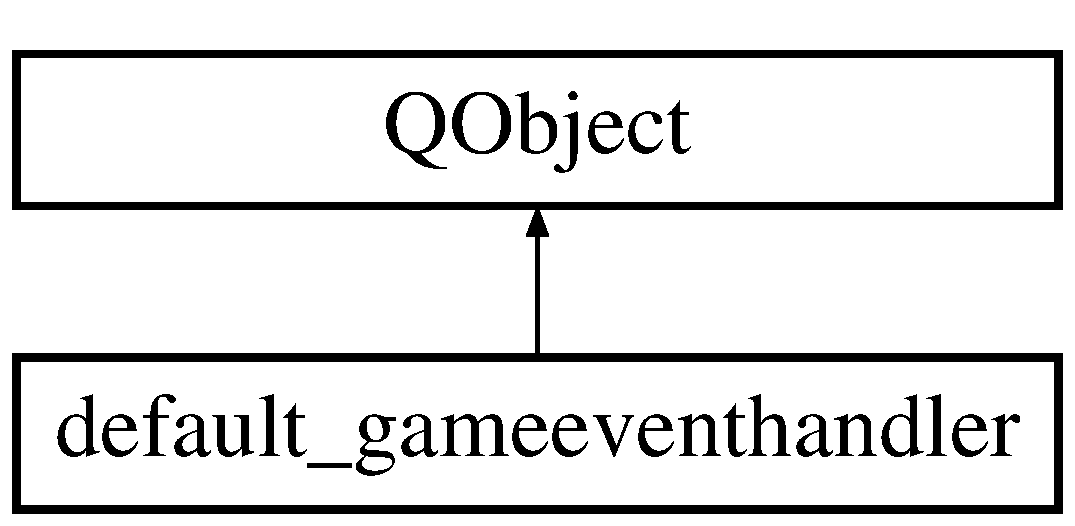
\includegraphics[height=2.000000cm]{classdefault__gameeventhandler}
\end{center}
\end{figure}
\subsection*{Public Member Functions}
\begin{DoxyCompactItemize}
\item 
\hyperlink{classdefault__gameeventhandler_a95b0dc5a9a792c26221332de6008ed1a}{default\-\_\-gameeventhandler} ()
\begin{DoxyCompactList}\small\item\em Test setup. \end{DoxyCompactList}\end{DoxyCompactItemize}
\subsection*{Private Slots}
\begin{DoxyCompactItemize}
\item 
void \hyperlink{classdefault__gameeventhandler_af32f4c295555f30b7d922d1c55399e91}{test\-\_\-player\-Has\-Won} ()
\begin{DoxyCompactList}\small\item\em Tests player reaching the win condition. \end{DoxyCompactList}\item 
void \hyperlink{classdefault__gameeventhandler_a3eb2c5de5b08c3217a04d6b45d3b255b}{test\-\_\-modify\-Resource} ()
\begin{DoxyCompactList}\small\item\em Tests modifying a player's resource. \end{DoxyCompactList}\item 
void \hyperlink{classdefault__gameeventhandler_a17c006978a06fc12a6b88b3c1814e11c}{test\-\_\-modify\-Resources} ()
\begin{DoxyCompactList}\small\item\em Tests modifying a player's resources. \end{DoxyCompactList}\item 
void \hyperlink{classdefault__gameeventhandler_aa0b383fd6c699b1f044022bfe5269d2b}{test\-\_\-player\-In\-Turn} ()
\begin{DoxyCompactList}\small\item\em Tests getting and setting the player in turn. \end{DoxyCompactList}\item 
void \hyperlink{classdefault__gameeventhandler_a253bd1627b80b1259b2a1c30701e428c}{test\-\_\-is\-Buying} ()
\begin{DoxyCompactList}\small\item\em Tests getting and setting the buying-\/flag. \end{DoxyCompactList}\item 
void \hyperlink{classdefault__gameeventhandler_aaccee5017653e8216f2193c926e81265}{test\-\_\-rounds} ()
\begin{DoxyCompactList}\small\item\em Tests getting and increasing the current game round. \end{DoxyCompactList}\item 
void \hyperlink{classdefault__gameeventhandler_ab933cc221885e1793129cbe57e149c32}{cleanup} ()
\begin{DoxyCompactList}\small\item\em Test cleanup. \end{DoxyCompactList}\end{DoxyCompactItemize}
\subsection*{Private Attributes}
\begin{DoxyCompactItemize}
\item 
std\-::shared\-\_\-ptr$<$ \hyperlink{classGame_1_1ObjectManager}{Object\-Manager} $>$ \hyperlink{classdefault__gameeventhandler_acdd2478cf08de20b164b66ec103b7de1}{obj\-Man}
\item 
std\-::shared\-\_\-ptr$<$ \hyperlink{classGame_1_1GameEventHandler}{Game\-Event\-Handler} $>$ \hyperlink{classdefault__gameeventhandler_aefeb6dad4999cfc75af77e989043815c}{gameeventhandler\-\_\-object}
\item 
int \hyperlink{classdefault__gameeventhandler_a1ac8cedd79456662813fa56454501d88}{win\-Resource\-Sum}
\item 
\hyperlink{namespaceCourse_ab9a46ed9cd00485e318e5731ea2f78d9}{Course\-::\-Resource\-Map} \hyperlink{classdefault__gameeventhandler_a09d45dc3340790f910f4c42a200d5fbf}{zero\-Resources}
\item 
\hyperlink{namespaceCourse_ab9a46ed9cd00485e318e5731ea2f78d9}{Course\-::\-Resource\-Map} \hyperlink{classdefault__gameeventhandler_aa6df2098d736982fb23603eff7edcf02}{start\-Resources}
\item 
\hyperlink{namespaceCourse_ab9a46ed9cd00485e318e5731ea2f78d9}{Course\-::\-Resource\-Map} \hyperlink{classdefault__gameeventhandler_aa22ed639196433fa97c3c53501660910}{minus\-Start\-Resources}
\item 
std\-::shared\-\_\-ptr$<$ \hyperlink{classGame_1_1Player}{Player} $>$ \hyperlink{classdefault__gameeventhandler_a25fc82697d08eb776919e8286bd2db5d}{player1}
\item 
std\-::shared\-\_\-ptr$<$ \hyperlink{classGame_1_1Player}{Player} $>$ \hyperlink{classdefault__gameeventhandler_a638662f415f3dc219ebb727b546734ba}{player2}
\end{DoxyCompactItemize}


\subsection{Detailed Description}
The gameventhandler\-\_\-tests test the Game\-Event\-Handler class. 

\subsection{Constructor \& Destructor Documentation}
\hypertarget{classdefault__gameeventhandler_a95b0dc5a9a792c26221332de6008ed1a}{\index{default\-\_\-gameeventhandler@{default\-\_\-gameeventhandler}!default\-\_\-gameeventhandler@{default\-\_\-gameeventhandler}}
\index{default\-\_\-gameeventhandler@{default\-\_\-gameeventhandler}!default_gameeventhandler@{default\-\_\-gameeventhandler}}
\subsubsection[{default\-\_\-gameeventhandler}]{\setlength{\rightskip}{0pt plus 5cm}default\-\_\-gameeventhandler\-::default\-\_\-gameeventhandler (
\begin{DoxyParamCaption}
{}
\end{DoxyParamCaption}
)}}\label{classdefault__gameeventhandler_a95b0dc5a9a792c26221332de6008ed1a}


Test setup. 



\subsection{Member Function Documentation}
\hypertarget{classdefault__gameeventhandler_ab933cc221885e1793129cbe57e149c32}{\index{default\-\_\-gameeventhandler@{default\-\_\-gameeventhandler}!cleanup@{cleanup}}
\index{cleanup@{cleanup}!default_gameeventhandler@{default\-\_\-gameeventhandler}}
\subsubsection[{cleanup}]{\setlength{\rightskip}{0pt plus 5cm}void default\-\_\-gameeventhandler\-::cleanup (
\begin{DoxyParamCaption}
{}
\end{DoxyParamCaption}
)\hspace{0.3cm}{\ttfamily [private]}, {\ttfamily [slot]}}}\label{classdefault__gameeventhandler_ab933cc221885e1793129cbe57e149c32}


Test cleanup. 

\hypertarget{classdefault__gameeventhandler_a253bd1627b80b1259b2a1c30701e428c}{\index{default\-\_\-gameeventhandler@{default\-\_\-gameeventhandler}!test\-\_\-is\-Buying@{test\-\_\-is\-Buying}}
\index{test\-\_\-is\-Buying@{test\-\_\-is\-Buying}!default_gameeventhandler@{default\-\_\-gameeventhandler}}
\subsubsection[{test\-\_\-is\-Buying}]{\setlength{\rightskip}{0pt plus 5cm}void default\-\_\-gameeventhandler\-::test\-\_\-is\-Buying (
\begin{DoxyParamCaption}
{}
\end{DoxyParamCaption}
)\hspace{0.3cm}{\ttfamily [private]}, {\ttfamily [slot]}}}\label{classdefault__gameeventhandler_a253bd1627b80b1259b2a1c30701e428c}


Tests getting and setting the buying-\/flag. 

\begin{DoxyPostcond}{Postcondition}
Buying flag should change and be returned correctly 
\end{DoxyPostcond}
\hypertarget{classdefault__gameeventhandler_a3eb2c5de5b08c3217a04d6b45d3b255b}{\index{default\-\_\-gameeventhandler@{default\-\_\-gameeventhandler}!test\-\_\-modify\-Resource@{test\-\_\-modify\-Resource}}
\index{test\-\_\-modify\-Resource@{test\-\_\-modify\-Resource}!default_gameeventhandler@{default\-\_\-gameeventhandler}}
\subsubsection[{test\-\_\-modify\-Resource}]{\setlength{\rightskip}{0pt plus 5cm}void default\-\_\-gameeventhandler\-::test\-\_\-modify\-Resource (
\begin{DoxyParamCaption}
{}
\end{DoxyParamCaption}
)\hspace{0.3cm}{\ttfamily [private]}, {\ttfamily [slot]}}}\label{classdefault__gameeventhandler_a3eb2c5de5b08c3217a04d6b45d3b255b}


Tests modifying a player's resource. 

\begin{DoxyPostcond}{Postcondition}
Resource should be modified accordingly 
\end{DoxyPostcond}
\hypertarget{classdefault__gameeventhandler_a17c006978a06fc12a6b88b3c1814e11c}{\index{default\-\_\-gameeventhandler@{default\-\_\-gameeventhandler}!test\-\_\-modify\-Resources@{test\-\_\-modify\-Resources}}
\index{test\-\_\-modify\-Resources@{test\-\_\-modify\-Resources}!default_gameeventhandler@{default\-\_\-gameeventhandler}}
\subsubsection[{test\-\_\-modify\-Resources}]{\setlength{\rightskip}{0pt plus 5cm}void default\-\_\-gameeventhandler\-::test\-\_\-modify\-Resources (
\begin{DoxyParamCaption}
{}
\end{DoxyParamCaption}
)\hspace{0.3cm}{\ttfamily [private]}, {\ttfamily [slot]}}}\label{classdefault__gameeventhandler_a17c006978a06fc12a6b88b3c1814e11c}


Tests modifying a player's resources. 

\begin{DoxyPostcond}{Postcondition}
Resources should be modified accordingly 
\end{DoxyPostcond}
\hypertarget{classdefault__gameeventhandler_af32f4c295555f30b7d922d1c55399e91}{\index{default\-\_\-gameeventhandler@{default\-\_\-gameeventhandler}!test\-\_\-player\-Has\-Won@{test\-\_\-player\-Has\-Won}}
\index{test\-\_\-player\-Has\-Won@{test\-\_\-player\-Has\-Won}!default_gameeventhandler@{default\-\_\-gameeventhandler}}
\subsubsection[{test\-\_\-player\-Has\-Won}]{\setlength{\rightskip}{0pt plus 5cm}void default\-\_\-gameeventhandler\-::test\-\_\-player\-Has\-Won (
\begin{DoxyParamCaption}
{}
\end{DoxyParamCaption}
)\hspace{0.3cm}{\ttfamily [private]}, {\ttfamily [slot]}}}\label{classdefault__gameeventhandler_af32f4c295555f30b7d922d1c55399e91}


Tests player reaching the win condition. 

\begin{DoxyPostcond}{Postcondition}
Player should be selected as the winner 
\end{DoxyPostcond}
\hypertarget{classdefault__gameeventhandler_aa0b383fd6c699b1f044022bfe5269d2b}{\index{default\-\_\-gameeventhandler@{default\-\_\-gameeventhandler}!test\-\_\-player\-In\-Turn@{test\-\_\-player\-In\-Turn}}
\index{test\-\_\-player\-In\-Turn@{test\-\_\-player\-In\-Turn}!default_gameeventhandler@{default\-\_\-gameeventhandler}}
\subsubsection[{test\-\_\-player\-In\-Turn}]{\setlength{\rightskip}{0pt plus 5cm}void default\-\_\-gameeventhandler\-::test\-\_\-player\-In\-Turn (
\begin{DoxyParamCaption}
{}
\end{DoxyParamCaption}
)\hspace{0.3cm}{\ttfamily [private]}, {\ttfamily [slot]}}}\label{classdefault__gameeventhandler_aa0b383fd6c699b1f044022bfe5269d2b}


Tests getting and setting the player in turn. 

\begin{DoxyPostcond}{Postcondition}
Player in turn should change and be returned correctly 
\end{DoxyPostcond}
\hypertarget{classdefault__gameeventhandler_aaccee5017653e8216f2193c926e81265}{\index{default\-\_\-gameeventhandler@{default\-\_\-gameeventhandler}!test\-\_\-rounds@{test\-\_\-rounds}}
\index{test\-\_\-rounds@{test\-\_\-rounds}!default_gameeventhandler@{default\-\_\-gameeventhandler}}
\subsubsection[{test\-\_\-rounds}]{\setlength{\rightskip}{0pt plus 5cm}void default\-\_\-gameeventhandler\-::test\-\_\-rounds (
\begin{DoxyParamCaption}
{}
\end{DoxyParamCaption}
)\hspace{0.3cm}{\ttfamily [private]}, {\ttfamily [slot]}}}\label{classdefault__gameeventhandler_aaccee5017653e8216f2193c926e81265}


Tests getting and increasing the current game round. 

\begin{DoxyPostcond}{Postcondition}
Rounds should increase and be returned correctly 
\end{DoxyPostcond}


\subsection{Member Data Documentation}
\hypertarget{classdefault__gameeventhandler_aefeb6dad4999cfc75af77e989043815c}{\index{default\-\_\-gameeventhandler@{default\-\_\-gameeventhandler}!gameeventhandler\-\_\-object@{gameeventhandler\-\_\-object}}
\index{gameeventhandler\-\_\-object@{gameeventhandler\-\_\-object}!default_gameeventhandler@{default\-\_\-gameeventhandler}}
\subsubsection[{gameeventhandler\-\_\-object}]{\setlength{\rightskip}{0pt plus 5cm}std\-::shared\-\_\-ptr$<${\bf Game\-Event\-Handler}$>$ default\-\_\-gameeventhandler\-::gameeventhandler\-\_\-object\hspace{0.3cm}{\ttfamily [private]}}}\label{classdefault__gameeventhandler_aefeb6dad4999cfc75af77e989043815c}
\hypertarget{classdefault__gameeventhandler_aa22ed639196433fa97c3c53501660910}{\index{default\-\_\-gameeventhandler@{default\-\_\-gameeventhandler}!minus\-Start\-Resources@{minus\-Start\-Resources}}
\index{minus\-Start\-Resources@{minus\-Start\-Resources}!default_gameeventhandler@{default\-\_\-gameeventhandler}}
\subsubsection[{minus\-Start\-Resources}]{\setlength{\rightskip}{0pt plus 5cm}{\bf Course\-::\-Resource\-Map} default\-\_\-gameeventhandler\-::minus\-Start\-Resources\hspace{0.3cm}{\ttfamily [private]}}}\label{classdefault__gameeventhandler_aa22ed639196433fa97c3c53501660910}
\hypertarget{classdefault__gameeventhandler_acdd2478cf08de20b164b66ec103b7de1}{\index{default\-\_\-gameeventhandler@{default\-\_\-gameeventhandler}!obj\-Man@{obj\-Man}}
\index{obj\-Man@{obj\-Man}!default_gameeventhandler@{default\-\_\-gameeventhandler}}
\subsubsection[{obj\-Man}]{\setlength{\rightskip}{0pt plus 5cm}std\-::shared\-\_\-ptr$<${\bf Object\-Manager}$>$ default\-\_\-gameeventhandler\-::obj\-Man\hspace{0.3cm}{\ttfamily [private]}}}\label{classdefault__gameeventhandler_acdd2478cf08de20b164b66ec103b7de1}
\hypertarget{classdefault__gameeventhandler_a25fc82697d08eb776919e8286bd2db5d}{\index{default\-\_\-gameeventhandler@{default\-\_\-gameeventhandler}!player1@{player1}}
\index{player1@{player1}!default_gameeventhandler@{default\-\_\-gameeventhandler}}
\subsubsection[{player1}]{\setlength{\rightskip}{0pt plus 5cm}std\-::shared\-\_\-ptr$<${\bf Player}$>$ default\-\_\-gameeventhandler\-::player1\hspace{0.3cm}{\ttfamily [private]}}}\label{classdefault__gameeventhandler_a25fc82697d08eb776919e8286bd2db5d}
\hypertarget{classdefault__gameeventhandler_a638662f415f3dc219ebb727b546734ba}{\index{default\-\_\-gameeventhandler@{default\-\_\-gameeventhandler}!player2@{player2}}
\index{player2@{player2}!default_gameeventhandler@{default\-\_\-gameeventhandler}}
\subsubsection[{player2}]{\setlength{\rightskip}{0pt plus 5cm}std\-::shared\-\_\-ptr$<${\bf Player}$>$ default\-\_\-gameeventhandler\-::player2\hspace{0.3cm}{\ttfamily [private]}}}\label{classdefault__gameeventhandler_a638662f415f3dc219ebb727b546734ba}
\hypertarget{classdefault__gameeventhandler_aa6df2098d736982fb23603eff7edcf02}{\index{default\-\_\-gameeventhandler@{default\-\_\-gameeventhandler}!start\-Resources@{start\-Resources}}
\index{start\-Resources@{start\-Resources}!default_gameeventhandler@{default\-\_\-gameeventhandler}}
\subsubsection[{start\-Resources}]{\setlength{\rightskip}{0pt plus 5cm}{\bf Course\-::\-Resource\-Map} default\-\_\-gameeventhandler\-::start\-Resources\hspace{0.3cm}{\ttfamily [private]}}}\label{classdefault__gameeventhandler_aa6df2098d736982fb23603eff7edcf02}
\hypertarget{classdefault__gameeventhandler_a1ac8cedd79456662813fa56454501d88}{\index{default\-\_\-gameeventhandler@{default\-\_\-gameeventhandler}!win\-Resource\-Sum@{win\-Resource\-Sum}}
\index{win\-Resource\-Sum@{win\-Resource\-Sum}!default_gameeventhandler@{default\-\_\-gameeventhandler}}
\subsubsection[{win\-Resource\-Sum}]{\setlength{\rightskip}{0pt plus 5cm}int default\-\_\-gameeventhandler\-::win\-Resource\-Sum\hspace{0.3cm}{\ttfamily [private]}}}\label{classdefault__gameeventhandler_a1ac8cedd79456662813fa56454501d88}
\hypertarget{classdefault__gameeventhandler_a09d45dc3340790f910f4c42a200d5fbf}{\index{default\-\_\-gameeventhandler@{default\-\_\-gameeventhandler}!zero\-Resources@{zero\-Resources}}
\index{zero\-Resources@{zero\-Resources}!default_gameeventhandler@{default\-\_\-gameeventhandler}}
\subsubsection[{zero\-Resources}]{\setlength{\rightskip}{0pt plus 5cm}{\bf Course\-::\-Resource\-Map} default\-\_\-gameeventhandler\-::zero\-Resources\hspace{0.3cm}{\ttfamily [private]}}}\label{classdefault__gameeventhandler_a09d45dc3340790f910f4c42a200d5fbf}


The documentation for this class was generated from the following file\-:\begin{DoxyCompactItemize}
\item 
Unit\-Tests/gameeventhandler\-\_\-tests/\hyperlink{tst__default__gameeventhandler_8cpp}{tst\-\_\-default\-\_\-gameeventhandler.\-cpp}\end{DoxyCompactItemize}

\hypertarget{classdefault__gameobjects}{\section{default\-\_\-gameobjects Class Reference}
\label{classdefault__gameobjects}\index{default\-\_\-gameobjects@{default\-\_\-gameobjects}}
}
Inheritance diagram for default\-\_\-gameobjects\-:\begin{figure}[H]
\begin{center}
\leavevmode
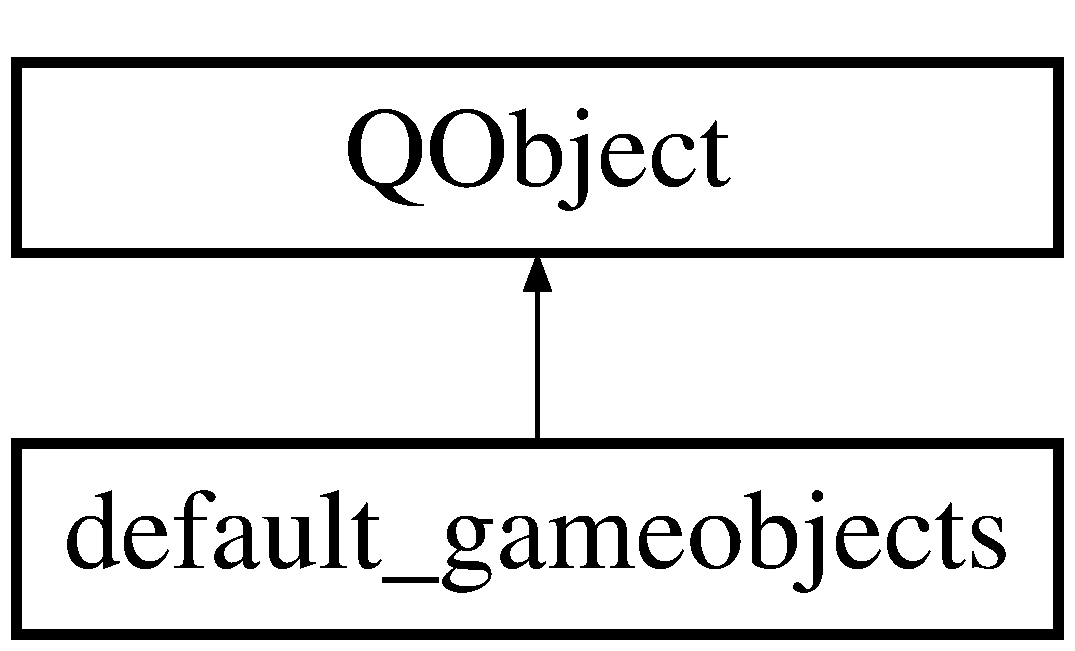
\includegraphics[height=2.000000cm]{classdefault__gameobjects}
\end{center}
\end{figure}
\subsection*{Public Member Functions}
\begin{DoxyCompactItemize}
\item 
\hyperlink{classdefault__gameobjects_a22d600cef773dfca6c6f3eca61d5ea10}{default\-\_\-gameobjects} ()
\item 
\hyperlink{classdefault__gameobjects_a384c1eb52e64799bc9a8416bc9e4c8af}{$\sim$default\-\_\-gameobjects} ()
\end{DoxyCompactItemize}
\subsection*{Private Slots}
\begin{DoxyCompactItemize}
\item 
void \hyperlink{classdefault__gameobjects_a1b2f12a75a6fd560d34f32b5ba0f34da}{test\-\_\-set\-Owner} ()
\item 
void \hyperlink{classdefault__gameobjects_aaa9c0152f449c606500cf96690ae3c13}{test\-\_\-set\-Coordinate\-\_\-from\-\_\-shared\-\_\-ptr} ()
\item 
void \hyperlink{classdefault__gameobjects_a0883afe617123263ad602f87fa983683}{test\-\_\-set\-Coordinate\-\_\-from\-\_\-instance} ()
\item 
void \hyperlink{classdefault__gameobjects_af2580d926eca2aa41826048b3726fc4f}{test\-\_\-unset\-Coordinate} ()
\item 
void \hyperlink{classdefault__gameobjects_a2ab3a9693bab4ec2e85cba63caa0785e}{test\-\_\-set\-Description} ()
\item 
void \hyperlink{classdefault__gameobjects_afdd9756c0869ae023c8c45fb69461398}{test\-\_\-set\-Descriptions} ()
\item 
void \hyperlink{classdefault__gameobjects_a75efd7811b51bb6ec4cb25d72f4421f0}{test\-\_\-add\-Description} ()
\item 
void \hyperlink{classdefault__gameobjects_af802e807c97f51c84bc85d5014d556e0}{test\-\_\-add\-Description\-\_\-exception} ()
\item 
void \hyperlink{classdefault__gameobjects_a5f1f3f3f10bcee841f5382ecd7a4e105}{test\-\_\-remove\-Description} ()
\item 
void \hyperlink{classdefault__gameobjects_aaa05cc0bc58d54582a72fb6b457fd01c}{test\-\_\-remove\-Description\-\_\-exception} ()
\item 
void \hyperlink{classdefault__gameobjects_a38dba54182b375ed1592ef3938bb7dbe}{test\-\_\-clear\-Descriptions} ()
\item 
void \hyperlink{classdefault__gameobjects_ae344b74fe80ba55e68709e9ef01291fa}{test\-\_\-get\-Description} ()
\item 
void \hyperlink{classdefault__gameobjects_aa30ca9e1cf57f614e04e0dea59cd4b46}{test\-\_\-get\-Description\-\_\-exception} ()
\item 
void \hyperlink{classdefault__gameobjects_ad7edaff14ef790a4b4ad005398d63c50}{cleanup} ()
\end{DoxyCompactItemize}
\subsection*{Private Member Functions}
\begin{DoxyCompactItemize}
\item 
bool \hyperlink{classdefault__gameobjects_af7997108c7d76177f670658c155bdbfb}{description\-Maps\-Match} (const \hyperlink{namespaceCourse_aed04c39dde5a591d4b353686d3d0e306}{Description\-Map} \&l, const \hyperlink{namespaceCourse_aed04c39dde5a591d4b353686d3d0e306}{Description\-Map} \&r)
\end{DoxyCompactItemize}
\subsection*{Private Attributes}
\begin{DoxyCompactItemize}
\item 
const std\-::string \hyperlink{classdefault__gameobjects_a0bdbe26cd36718ba9c628747c5323c55}{D\-E\-F\-\_\-\-P\-L\-A\-Y\-E\-R\-\_\-\-N\-A\-M\-E} = \char`\"{}Player 1\char`\"{}
\item 
const \hyperlink{namespaceCourse_aed04c39dde5a591d4b353686d3d0e306}{Description\-Map} \hyperlink{classdefault__gameobjects_abbebe0d0ab551b8e54391e90b360a514}{D\-E\-F\-\_\-\-D\-E\-S\-C\-R\-I\-P\-T\-I\-O\-N\-S}
\item 
const int \hyperlink{classdefault__gameobjects_a3d0f2d4c4dae2ebed8a97f4f1433bc31}{D\-E\-F\-\_\-\-C\-O\-O\-R\-D\-I\-N\-A\-T\-E\-\_\-\-X} = 0
\item 
const int \hyperlink{classdefault__gameobjects_aa473544da0a7d14b8f8f4e2e4b696441}{D\-E\-F\-\_\-\-C\-O\-O\-R\-D\-I\-N\-A\-T\-E\-\_\-\-Y} = 0
\item 
std\-::unique\-\_\-ptr$<$ \hyperlink{classCourse_1_1GameObject}{Game\-Object} $>$ \hyperlink{classdefault__gameobjects_a4dfa6f390ff4c2c331c342b6c88b16d7}{default\-\_\-instance}
\item 
std\-::shared\-\_\-ptr$<$ \hyperlink{classCourse_1_1PlayerBase}{Player\-Base} $>$ \hyperlink{classdefault__gameobjects_a66ae835be72c7ce9cc5cec3970cb0834}{def\-\_\-player}
\item 
std\-::shared\-\_\-ptr$<$ \hyperlink{classCourse_1_1Coordinate}{Coordinate} $>$ \hyperlink{classdefault__gameobjects_af9e1d7eca682f17b97659d34b973a1b6}{def\-\_\-coordinate}
\end{DoxyCompactItemize}


\subsection{Constructor \& Destructor Documentation}
\hypertarget{classdefault__gameobjects_a22d600cef773dfca6c6f3eca61d5ea10}{\index{default\-\_\-gameobjects@{default\-\_\-gameobjects}!default\-\_\-gameobjects@{default\-\_\-gameobjects}}
\index{default\-\_\-gameobjects@{default\-\_\-gameobjects}!default_gameobjects@{default\-\_\-gameobjects}}
\subsubsection[{default\-\_\-gameobjects}]{\setlength{\rightskip}{0pt plus 5cm}default\-\_\-gameobjects\-::default\-\_\-gameobjects (
\begin{DoxyParamCaption}
{}
\end{DoxyParamCaption}
)}}\label{classdefault__gameobjects_a22d600cef773dfca6c6f3eca61d5ea10}
\hypertarget{classdefault__gameobjects_a384c1eb52e64799bc9a8416bc9e4c8af}{\index{default\-\_\-gameobjects@{default\-\_\-gameobjects}!$\sim$default\-\_\-gameobjects@{$\sim$default\-\_\-gameobjects}}
\index{$\sim$default\-\_\-gameobjects@{$\sim$default\-\_\-gameobjects}!default_gameobjects@{default\-\_\-gameobjects}}
\subsubsection[{$\sim$default\-\_\-gameobjects}]{\setlength{\rightskip}{0pt plus 5cm}default\-\_\-gameobjects\-::$\sim$default\-\_\-gameobjects (
\begin{DoxyParamCaption}
{}
\end{DoxyParamCaption}
)}}\label{classdefault__gameobjects_a384c1eb52e64799bc9a8416bc9e4c8af}


\subsection{Member Function Documentation}
\hypertarget{classdefault__gameobjects_ad7edaff14ef790a4b4ad005398d63c50}{\index{default\-\_\-gameobjects@{default\-\_\-gameobjects}!cleanup@{cleanup}}
\index{cleanup@{cleanup}!default_gameobjects@{default\-\_\-gameobjects}}
\subsubsection[{cleanup}]{\setlength{\rightskip}{0pt plus 5cm}void default\-\_\-gameobjects\-::cleanup (
\begin{DoxyParamCaption}
{}
\end{DoxyParamCaption}
)\hspace{0.3cm}{\ttfamily [private]}, {\ttfamily [slot]}}}\label{classdefault__gameobjects_ad7edaff14ef790a4b4ad005398d63c50}
\hypertarget{classdefault__gameobjects_af7997108c7d76177f670658c155bdbfb}{\index{default\-\_\-gameobjects@{default\-\_\-gameobjects}!description\-Maps\-Match@{description\-Maps\-Match}}
\index{description\-Maps\-Match@{description\-Maps\-Match}!default_gameobjects@{default\-\_\-gameobjects}}
\subsubsection[{description\-Maps\-Match}]{\setlength{\rightskip}{0pt plus 5cm}bool default\-\_\-gameobjects\-::description\-Maps\-Match (
\begin{DoxyParamCaption}
\item[{const {\bf Description\-Map} \&}]{l, }
\item[{const {\bf Description\-Map} \&}]{r}
\end{DoxyParamCaption}
)\hspace{0.3cm}{\ttfamily [private]}}}\label{classdefault__gameobjects_af7997108c7d76177f670658c155bdbfb}
\hypertarget{classdefault__gameobjects_a75efd7811b51bb6ec4cb25d72f4421f0}{\index{default\-\_\-gameobjects@{default\-\_\-gameobjects}!test\-\_\-add\-Description@{test\-\_\-add\-Description}}
\index{test\-\_\-add\-Description@{test\-\_\-add\-Description}!default_gameobjects@{default\-\_\-gameobjects}}
\subsubsection[{test\-\_\-add\-Description}]{\setlength{\rightskip}{0pt plus 5cm}void default\-\_\-gameobjects\-::test\-\_\-add\-Description (
\begin{DoxyParamCaption}
{}
\end{DoxyParamCaption}
)\hspace{0.3cm}{\ttfamily [private]}, {\ttfamily [slot]}}}\label{classdefault__gameobjects_a75efd7811b51bb6ec4cb25d72f4421f0}
\hypertarget{classdefault__gameobjects_af802e807c97f51c84bc85d5014d556e0}{\index{default\-\_\-gameobjects@{default\-\_\-gameobjects}!test\-\_\-add\-Description\-\_\-exception@{test\-\_\-add\-Description\-\_\-exception}}
\index{test\-\_\-add\-Description\-\_\-exception@{test\-\_\-add\-Description\-\_\-exception}!default_gameobjects@{default\-\_\-gameobjects}}
\subsubsection[{test\-\_\-add\-Description\-\_\-exception}]{\setlength{\rightskip}{0pt plus 5cm}void default\-\_\-gameobjects\-::test\-\_\-add\-Description\-\_\-exception (
\begin{DoxyParamCaption}
{}
\end{DoxyParamCaption}
)\hspace{0.3cm}{\ttfamily [private]}, {\ttfamily [slot]}}}\label{classdefault__gameobjects_af802e807c97f51c84bc85d5014d556e0}
\hypertarget{classdefault__gameobjects_a38dba54182b375ed1592ef3938bb7dbe}{\index{default\-\_\-gameobjects@{default\-\_\-gameobjects}!test\-\_\-clear\-Descriptions@{test\-\_\-clear\-Descriptions}}
\index{test\-\_\-clear\-Descriptions@{test\-\_\-clear\-Descriptions}!default_gameobjects@{default\-\_\-gameobjects}}
\subsubsection[{test\-\_\-clear\-Descriptions}]{\setlength{\rightskip}{0pt plus 5cm}void default\-\_\-gameobjects\-::test\-\_\-clear\-Descriptions (
\begin{DoxyParamCaption}
{}
\end{DoxyParamCaption}
)\hspace{0.3cm}{\ttfamily [private]}, {\ttfamily [slot]}}}\label{classdefault__gameobjects_a38dba54182b375ed1592ef3938bb7dbe}
\hypertarget{classdefault__gameobjects_ae344b74fe80ba55e68709e9ef01291fa}{\index{default\-\_\-gameobjects@{default\-\_\-gameobjects}!test\-\_\-get\-Description@{test\-\_\-get\-Description}}
\index{test\-\_\-get\-Description@{test\-\_\-get\-Description}!default_gameobjects@{default\-\_\-gameobjects}}
\subsubsection[{test\-\_\-get\-Description}]{\setlength{\rightskip}{0pt plus 5cm}void default\-\_\-gameobjects\-::test\-\_\-get\-Description (
\begin{DoxyParamCaption}
{}
\end{DoxyParamCaption}
)\hspace{0.3cm}{\ttfamily [private]}, {\ttfamily [slot]}}}\label{classdefault__gameobjects_ae344b74fe80ba55e68709e9ef01291fa}
\hypertarget{classdefault__gameobjects_aa30ca9e1cf57f614e04e0dea59cd4b46}{\index{default\-\_\-gameobjects@{default\-\_\-gameobjects}!test\-\_\-get\-Description\-\_\-exception@{test\-\_\-get\-Description\-\_\-exception}}
\index{test\-\_\-get\-Description\-\_\-exception@{test\-\_\-get\-Description\-\_\-exception}!default_gameobjects@{default\-\_\-gameobjects}}
\subsubsection[{test\-\_\-get\-Description\-\_\-exception}]{\setlength{\rightskip}{0pt plus 5cm}void default\-\_\-gameobjects\-::test\-\_\-get\-Description\-\_\-exception (
\begin{DoxyParamCaption}
{}
\end{DoxyParamCaption}
)\hspace{0.3cm}{\ttfamily [private]}, {\ttfamily [slot]}}}\label{classdefault__gameobjects_aa30ca9e1cf57f614e04e0dea59cd4b46}
\hypertarget{classdefault__gameobjects_a5f1f3f3f10bcee841f5382ecd7a4e105}{\index{default\-\_\-gameobjects@{default\-\_\-gameobjects}!test\-\_\-remove\-Description@{test\-\_\-remove\-Description}}
\index{test\-\_\-remove\-Description@{test\-\_\-remove\-Description}!default_gameobjects@{default\-\_\-gameobjects}}
\subsubsection[{test\-\_\-remove\-Description}]{\setlength{\rightskip}{0pt plus 5cm}void default\-\_\-gameobjects\-::test\-\_\-remove\-Description (
\begin{DoxyParamCaption}
{}
\end{DoxyParamCaption}
)\hspace{0.3cm}{\ttfamily [private]}, {\ttfamily [slot]}}}\label{classdefault__gameobjects_a5f1f3f3f10bcee841f5382ecd7a4e105}
\hypertarget{classdefault__gameobjects_aaa05cc0bc58d54582a72fb6b457fd01c}{\index{default\-\_\-gameobjects@{default\-\_\-gameobjects}!test\-\_\-remove\-Description\-\_\-exception@{test\-\_\-remove\-Description\-\_\-exception}}
\index{test\-\_\-remove\-Description\-\_\-exception@{test\-\_\-remove\-Description\-\_\-exception}!default_gameobjects@{default\-\_\-gameobjects}}
\subsubsection[{test\-\_\-remove\-Description\-\_\-exception}]{\setlength{\rightskip}{0pt plus 5cm}void default\-\_\-gameobjects\-::test\-\_\-remove\-Description\-\_\-exception (
\begin{DoxyParamCaption}
{}
\end{DoxyParamCaption}
)\hspace{0.3cm}{\ttfamily [private]}, {\ttfamily [slot]}}}\label{classdefault__gameobjects_aaa05cc0bc58d54582a72fb6b457fd01c}
\hypertarget{classdefault__gameobjects_a0883afe617123263ad602f87fa983683}{\index{default\-\_\-gameobjects@{default\-\_\-gameobjects}!test\-\_\-set\-Coordinate\-\_\-from\-\_\-instance@{test\-\_\-set\-Coordinate\-\_\-from\-\_\-instance}}
\index{test\-\_\-set\-Coordinate\-\_\-from\-\_\-instance@{test\-\_\-set\-Coordinate\-\_\-from\-\_\-instance}!default_gameobjects@{default\-\_\-gameobjects}}
\subsubsection[{test\-\_\-set\-Coordinate\-\_\-from\-\_\-instance}]{\setlength{\rightskip}{0pt plus 5cm}void default\-\_\-gameobjects\-::test\-\_\-set\-Coordinate\-\_\-from\-\_\-instance (
\begin{DoxyParamCaption}
{}
\end{DoxyParamCaption}
)\hspace{0.3cm}{\ttfamily [private]}, {\ttfamily [slot]}}}\label{classdefault__gameobjects_a0883afe617123263ad602f87fa983683}
\hypertarget{classdefault__gameobjects_aaa9c0152f449c606500cf96690ae3c13}{\index{default\-\_\-gameobjects@{default\-\_\-gameobjects}!test\-\_\-set\-Coordinate\-\_\-from\-\_\-shared\-\_\-ptr@{test\-\_\-set\-Coordinate\-\_\-from\-\_\-shared\-\_\-ptr}}
\index{test\-\_\-set\-Coordinate\-\_\-from\-\_\-shared\-\_\-ptr@{test\-\_\-set\-Coordinate\-\_\-from\-\_\-shared\-\_\-ptr}!default_gameobjects@{default\-\_\-gameobjects}}
\subsubsection[{test\-\_\-set\-Coordinate\-\_\-from\-\_\-shared\-\_\-ptr}]{\setlength{\rightskip}{0pt plus 5cm}void default\-\_\-gameobjects\-::test\-\_\-set\-Coordinate\-\_\-from\-\_\-shared\-\_\-ptr (
\begin{DoxyParamCaption}
{}
\end{DoxyParamCaption}
)\hspace{0.3cm}{\ttfamily [private]}, {\ttfamily [slot]}}}\label{classdefault__gameobjects_aaa9c0152f449c606500cf96690ae3c13}
\hypertarget{classdefault__gameobjects_a2ab3a9693bab4ec2e85cba63caa0785e}{\index{default\-\_\-gameobjects@{default\-\_\-gameobjects}!test\-\_\-set\-Description@{test\-\_\-set\-Description}}
\index{test\-\_\-set\-Description@{test\-\_\-set\-Description}!default_gameobjects@{default\-\_\-gameobjects}}
\subsubsection[{test\-\_\-set\-Description}]{\setlength{\rightskip}{0pt plus 5cm}void default\-\_\-gameobjects\-::test\-\_\-set\-Description (
\begin{DoxyParamCaption}
{}
\end{DoxyParamCaption}
)\hspace{0.3cm}{\ttfamily [private]}, {\ttfamily [slot]}}}\label{classdefault__gameobjects_a2ab3a9693bab4ec2e85cba63caa0785e}
\hypertarget{classdefault__gameobjects_afdd9756c0869ae023c8c45fb69461398}{\index{default\-\_\-gameobjects@{default\-\_\-gameobjects}!test\-\_\-set\-Descriptions@{test\-\_\-set\-Descriptions}}
\index{test\-\_\-set\-Descriptions@{test\-\_\-set\-Descriptions}!default_gameobjects@{default\-\_\-gameobjects}}
\subsubsection[{test\-\_\-set\-Descriptions}]{\setlength{\rightskip}{0pt plus 5cm}void default\-\_\-gameobjects\-::test\-\_\-set\-Descriptions (
\begin{DoxyParamCaption}
{}
\end{DoxyParamCaption}
)\hspace{0.3cm}{\ttfamily [private]}, {\ttfamily [slot]}}}\label{classdefault__gameobjects_afdd9756c0869ae023c8c45fb69461398}
\hypertarget{classdefault__gameobjects_a1b2f12a75a6fd560d34f32b5ba0f34da}{\index{default\-\_\-gameobjects@{default\-\_\-gameobjects}!test\-\_\-set\-Owner@{test\-\_\-set\-Owner}}
\index{test\-\_\-set\-Owner@{test\-\_\-set\-Owner}!default_gameobjects@{default\-\_\-gameobjects}}
\subsubsection[{test\-\_\-set\-Owner}]{\setlength{\rightskip}{0pt plus 5cm}void default\-\_\-gameobjects\-::test\-\_\-set\-Owner (
\begin{DoxyParamCaption}
{}
\end{DoxyParamCaption}
)\hspace{0.3cm}{\ttfamily [private]}, {\ttfamily [slot]}}}\label{classdefault__gameobjects_a1b2f12a75a6fd560d34f32b5ba0f34da}
\hypertarget{classdefault__gameobjects_af2580d926eca2aa41826048b3726fc4f}{\index{default\-\_\-gameobjects@{default\-\_\-gameobjects}!test\-\_\-unset\-Coordinate@{test\-\_\-unset\-Coordinate}}
\index{test\-\_\-unset\-Coordinate@{test\-\_\-unset\-Coordinate}!default_gameobjects@{default\-\_\-gameobjects}}
\subsubsection[{test\-\_\-unset\-Coordinate}]{\setlength{\rightskip}{0pt plus 5cm}void default\-\_\-gameobjects\-::test\-\_\-unset\-Coordinate (
\begin{DoxyParamCaption}
{}
\end{DoxyParamCaption}
)\hspace{0.3cm}{\ttfamily [private]}, {\ttfamily [slot]}}}\label{classdefault__gameobjects_af2580d926eca2aa41826048b3726fc4f}


\subsection{Member Data Documentation}
\hypertarget{classdefault__gameobjects_af9e1d7eca682f17b97659d34b973a1b6}{\index{default\-\_\-gameobjects@{default\-\_\-gameobjects}!def\-\_\-coordinate@{def\-\_\-coordinate}}
\index{def\-\_\-coordinate@{def\-\_\-coordinate}!default_gameobjects@{default\-\_\-gameobjects}}
\subsubsection[{def\-\_\-coordinate}]{\setlength{\rightskip}{0pt plus 5cm}std\-::shared\-\_\-ptr$<${\bf Coordinate}$>$ default\-\_\-gameobjects\-::def\-\_\-coordinate\hspace{0.3cm}{\ttfamily [private]}}}\label{classdefault__gameobjects_af9e1d7eca682f17b97659d34b973a1b6}
\hypertarget{classdefault__gameobjects_a3d0f2d4c4dae2ebed8a97f4f1433bc31}{\index{default\-\_\-gameobjects@{default\-\_\-gameobjects}!D\-E\-F\-\_\-\-C\-O\-O\-R\-D\-I\-N\-A\-T\-E\-\_\-\-X@{D\-E\-F\-\_\-\-C\-O\-O\-R\-D\-I\-N\-A\-T\-E\-\_\-\-X}}
\index{D\-E\-F\-\_\-\-C\-O\-O\-R\-D\-I\-N\-A\-T\-E\-\_\-\-X@{D\-E\-F\-\_\-\-C\-O\-O\-R\-D\-I\-N\-A\-T\-E\-\_\-\-X}!default_gameobjects@{default\-\_\-gameobjects}}
\subsubsection[{D\-E\-F\-\_\-\-C\-O\-O\-R\-D\-I\-N\-A\-T\-E\-\_\-\-X}]{\setlength{\rightskip}{0pt plus 5cm}const int default\-\_\-gameobjects\-::\-D\-E\-F\-\_\-\-C\-O\-O\-R\-D\-I\-N\-A\-T\-E\-\_\-\-X = 0\hspace{0.3cm}{\ttfamily [private]}}}\label{classdefault__gameobjects_a3d0f2d4c4dae2ebed8a97f4f1433bc31}
\hypertarget{classdefault__gameobjects_aa473544da0a7d14b8f8f4e2e4b696441}{\index{default\-\_\-gameobjects@{default\-\_\-gameobjects}!D\-E\-F\-\_\-\-C\-O\-O\-R\-D\-I\-N\-A\-T\-E\-\_\-\-Y@{D\-E\-F\-\_\-\-C\-O\-O\-R\-D\-I\-N\-A\-T\-E\-\_\-\-Y}}
\index{D\-E\-F\-\_\-\-C\-O\-O\-R\-D\-I\-N\-A\-T\-E\-\_\-\-Y@{D\-E\-F\-\_\-\-C\-O\-O\-R\-D\-I\-N\-A\-T\-E\-\_\-\-Y}!default_gameobjects@{default\-\_\-gameobjects}}
\subsubsection[{D\-E\-F\-\_\-\-C\-O\-O\-R\-D\-I\-N\-A\-T\-E\-\_\-\-Y}]{\setlength{\rightskip}{0pt plus 5cm}const int default\-\_\-gameobjects\-::\-D\-E\-F\-\_\-\-C\-O\-O\-R\-D\-I\-N\-A\-T\-E\-\_\-\-Y = 0\hspace{0.3cm}{\ttfamily [private]}}}\label{classdefault__gameobjects_aa473544da0a7d14b8f8f4e2e4b696441}
\hypertarget{classdefault__gameobjects_abbebe0d0ab551b8e54391e90b360a514}{\index{default\-\_\-gameobjects@{default\-\_\-gameobjects}!D\-E\-F\-\_\-\-D\-E\-S\-C\-R\-I\-P\-T\-I\-O\-N\-S@{D\-E\-F\-\_\-\-D\-E\-S\-C\-R\-I\-P\-T\-I\-O\-N\-S}}
\index{D\-E\-F\-\_\-\-D\-E\-S\-C\-R\-I\-P\-T\-I\-O\-N\-S@{D\-E\-F\-\_\-\-D\-E\-S\-C\-R\-I\-P\-T\-I\-O\-N\-S}!default_gameobjects@{default\-\_\-gameobjects}}
\subsubsection[{D\-E\-F\-\_\-\-D\-E\-S\-C\-R\-I\-P\-T\-I\-O\-N\-S}]{\setlength{\rightskip}{0pt plus 5cm}const {\bf Description\-Map} default\-\_\-gameobjects\-::\-D\-E\-F\-\_\-\-D\-E\-S\-C\-R\-I\-P\-T\-I\-O\-N\-S\hspace{0.3cm}{\ttfamily [private]}}}\label{classdefault__gameobjects_abbebe0d0ab551b8e54391e90b360a514}
{\bfseries Initial value\-:}
\begin{DoxyCode}
= \{
        \{\textcolor{stringliteral}{"title"}, \textcolor{stringliteral}{"Default Object"}\},
        \{\textcolor{stringliteral}{"description"}, \textcolor{stringliteral}{"Like goggles, I do nothing."}\}
    \}
\end{DoxyCode}
\hypertarget{classdefault__gameobjects_a66ae835be72c7ce9cc5cec3970cb0834}{\index{default\-\_\-gameobjects@{default\-\_\-gameobjects}!def\-\_\-player@{def\-\_\-player}}
\index{def\-\_\-player@{def\-\_\-player}!default_gameobjects@{default\-\_\-gameobjects}}
\subsubsection[{def\-\_\-player}]{\setlength{\rightskip}{0pt plus 5cm}std\-::shared\-\_\-ptr$<${\bf Player\-Base}$>$ default\-\_\-gameobjects\-::def\-\_\-player\hspace{0.3cm}{\ttfamily [private]}}}\label{classdefault__gameobjects_a66ae835be72c7ce9cc5cec3970cb0834}
\hypertarget{classdefault__gameobjects_a0bdbe26cd36718ba9c628747c5323c55}{\index{default\-\_\-gameobjects@{default\-\_\-gameobjects}!D\-E\-F\-\_\-\-P\-L\-A\-Y\-E\-R\-\_\-\-N\-A\-M\-E@{D\-E\-F\-\_\-\-P\-L\-A\-Y\-E\-R\-\_\-\-N\-A\-M\-E}}
\index{D\-E\-F\-\_\-\-P\-L\-A\-Y\-E\-R\-\_\-\-N\-A\-M\-E@{D\-E\-F\-\_\-\-P\-L\-A\-Y\-E\-R\-\_\-\-N\-A\-M\-E}!default_gameobjects@{default\-\_\-gameobjects}}
\subsubsection[{D\-E\-F\-\_\-\-P\-L\-A\-Y\-E\-R\-\_\-\-N\-A\-M\-E}]{\setlength{\rightskip}{0pt plus 5cm}const std\-::string default\-\_\-gameobjects\-::\-D\-E\-F\-\_\-\-P\-L\-A\-Y\-E\-R\-\_\-\-N\-A\-M\-E = \char`\"{}Player 1\char`\"{}\hspace{0.3cm}{\ttfamily [private]}}}\label{classdefault__gameobjects_a0bdbe26cd36718ba9c628747c5323c55}
\hypertarget{classdefault__gameobjects_a4dfa6f390ff4c2c331c342b6c88b16d7}{\index{default\-\_\-gameobjects@{default\-\_\-gameobjects}!default\-\_\-instance@{default\-\_\-instance}}
\index{default\-\_\-instance@{default\-\_\-instance}!default_gameobjects@{default\-\_\-gameobjects}}
\subsubsection[{default\-\_\-instance}]{\setlength{\rightskip}{0pt plus 5cm}std\-::unique\-\_\-ptr$<${\bf Game\-Object}$>$ default\-\_\-gameobjects\-::default\-\_\-instance\hspace{0.3cm}{\ttfamily [private]}}}\label{classdefault__gameobjects_a4dfa6f390ff4c2c331c342b6c88b16d7}


The documentation for this class was generated from the following file\-:\begin{DoxyCompactItemize}
\item 
Course/\-Unit\-Tests/gameobject\-\_\-tests/\hyperlink{tst__default__gameobjects_8cpp}{tst\-\_\-default\-\_\-gameobjects.\-cpp}\end{DoxyCompactItemize}

\hypertarget{classdefault__objectmanager}{\section{default\-\_\-objectmanager Class Reference}
\label{classdefault__objectmanager}\index{default\-\_\-objectmanager@{default\-\_\-objectmanager}}
}


The objectmanager\-\_\-tests test the Object\-Manager class.  


Inheritance diagram for default\-\_\-objectmanager\-:\begin{figure}[H]
\begin{center}
\leavevmode
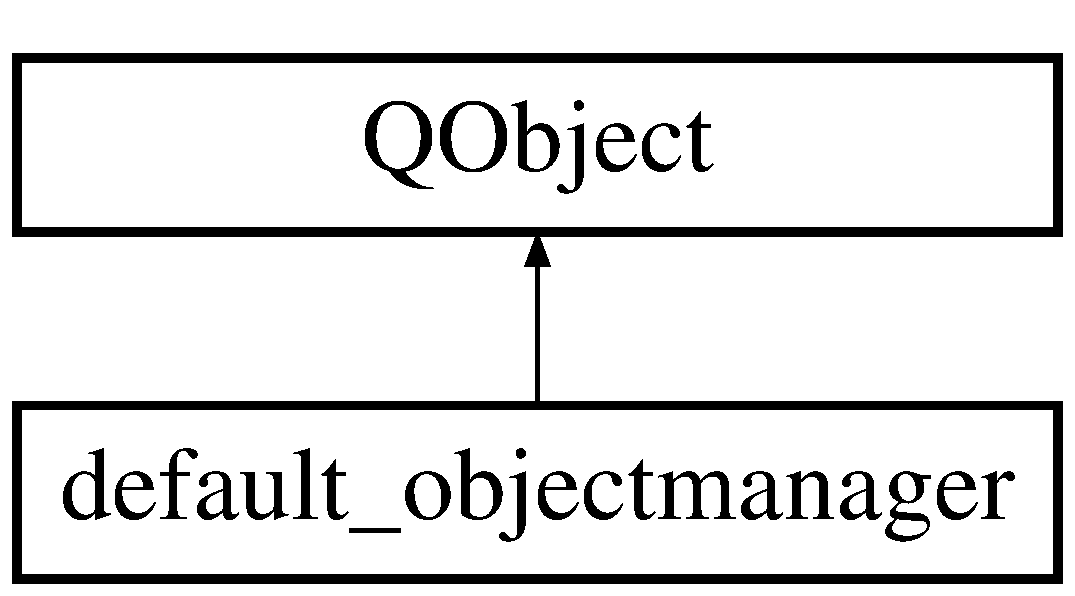
\includegraphics[height=2.000000cm]{classdefault__objectmanager}
\end{center}
\end{figure}
\subsection*{Public Member Functions}
\begin{DoxyCompactItemize}
\item 
\hyperlink{classdefault__objectmanager_ab59752a56a4ac34bc869403fbfbf6af6}{default\-\_\-objectmanager} ()
\begin{DoxyCompactList}\small\item\em Test setup. \end{DoxyCompactList}\end{DoxyCompactItemize}
\subsection*{Private Slots}
\begin{DoxyCompactItemize}
\item 
void \hyperlink{classdefault__objectmanager_aec7ac4004e9db71ce3b3437afa74dadf}{test\-\_\-player\-\_\-operations} ()
\begin{DoxyCompactList}\small\item\em Tests opeations to the list of players. \end{DoxyCompactList}\item 
void \hyperlink{classdefault__objectmanager_aab8dd175d96dfeba8c2220296e033dbd}{test\-\_\-tile\-\_\-operations} ()
\begin{DoxyCompactList}\small\item\em Tests opeations to the list of tiles. \end{DoxyCompactList}\item 
void \hyperlink{classdefault__objectmanager_a0ca24fa76077d630c473db1843412c43}{test\-\_\-placeableobject\-\_\-operations} ()
\begin{DoxyCompactList}\small\item\em Tests opeations to the list of placeableobjects \par
(workers and buildings) \end{DoxyCompactList}\item 
void \hyperlink{classdefault__objectmanager_a2ff9bd3c55983839dabc9ea9575990e0}{cleanup} ()
\begin{DoxyCompactList}\small\item\em Test cleanup. \end{DoxyCompactList}\end{DoxyCompactItemize}
\subsection*{Private Attributes}
\begin{DoxyCompactItemize}
\item 
std\-::shared\-\_\-ptr$<$ \hyperlink{classGame_1_1ObjectManager}{Object\-Manager} $>$ \hyperlink{classdefault__objectmanager_af5fd4a43346407b2813199cb58ba898d}{objectmanager\-\_\-object}
\item 
std\-::shared\-\_\-ptr$<$ \hyperlink{classGame_1_1GameEventHandler}{Game\-Event\-Handler} $>$ \hyperlink{classdefault__objectmanager_af3397bf426ecdc890c61d3d69701deff}{G\-E\-Hand}
\item 
int \hyperlink{classdefault__objectmanager_af38ed335952982ee29259ce5df67e18e}{win\-Resource\-Sum}
\item 
\hyperlink{namespaceCourse_ab9a46ed9cd00485e318e5731ea2f78d9}{Course\-::\-Resource\-Map} \hyperlink{classdefault__objectmanager_a86108da49a76801538881c75d2a395db}{zero\-Resources}
\item 
\hyperlink{namespaceCourse_ab9a46ed9cd00485e318e5731ea2f78d9}{Course\-::\-Resource\-Map} \hyperlink{classdefault__objectmanager_a228d3b342c250174d8f9924f6dd3d711}{start\-Resources}
\item 
\hyperlink{namespaceCourse_ab9a46ed9cd00485e318e5731ea2f78d9}{Course\-::\-Resource\-Map} \hyperlink{classdefault__objectmanager_a4a0cec3d5392cd32d7406877af357259}{minus\-Start\-Resources}
\item 
std\-::shared\-\_\-ptr$<$ \hyperlink{classGame_1_1Player}{Player} $>$ \hyperlink{classdefault__objectmanager_a1add15cff9927fa0ca0891d83db2aa66}{player1}
\item 
std\-::shared\-\_\-ptr$<$ \hyperlink{classGame_1_1Player}{Player} $>$ \hyperlink{classdefault__objectmanager_acd2b50e95f595209f088bffa2a5b0bf9}{player2}
\item 
std\-::shared\-\_\-ptr$<$ \hyperlink{classCourse_1_1TileBase}{Course\-::\-Tile\-Base} $>$ \hyperlink{classdefault__objectmanager_a083c627bb3cb830a59837af57933274e}{tile1}
\item 
std\-::shared\-\_\-ptr$<$ \hyperlink{classCourse_1_1TileBase}{Course\-::\-Tile\-Base} $>$ \hyperlink{classdefault__objectmanager_a822a88e652f6af04e9046f011844a12c}{tile2}
\item 
const \hyperlink{classCourse_1_1Coordinate}{Course\-::\-Coordinate} \hyperlink{classdefault__objectmanager_ac534d6d0d5db5425a0aeb95c84a6da17}{tile1\-\_\-coordinate} = \{1,1\}
\item 
const \hyperlink{classCourse_1_1Coordinate}{Course\-::\-Coordinate} \hyperlink{classdefault__objectmanager_a4c05b0c625dbbba4823e475d5cebc4d4}{tile2\-\_\-coordinate} = \{1,2\}
\item 
std\-::shared\-\_\-ptr\\*
$<$ \hyperlink{classCourse_1_1BuildingBase}{Course\-::\-Building\-Base} $>$ \hyperlink{classdefault__objectmanager_abfc94d530e7c532c632bac4f64c2e4b1}{building1}
\item 
std\-::shared\-\_\-ptr\\*
$<$ \hyperlink{classCourse_1_1BuildingBase}{Course\-::\-Building\-Base} $>$ \hyperlink{classdefault__objectmanager_a04dc230cada67d6d5ec7211bf95905f7}{building2}
\item 
std\-::shared\-\_\-ptr\\*
$<$ \hyperlink{classCourse_1_1BasicWorker}{Course\-::\-Basic\-Worker} $>$ \hyperlink{classdefault__objectmanager_a9372109fc55b6f04f2c6e5e888faa32c}{worker1}
\item 
std\-::shared\-\_\-ptr\\*
$<$ \hyperlink{classCourse_1_1BasicWorker}{Course\-::\-Basic\-Worker} $>$ \hyperlink{classdefault__objectmanager_aefff1e094b9f647478d960f1fbe0f897}{worker2}
\end{DoxyCompactItemize}


\subsection{Detailed Description}
The objectmanager\-\_\-tests test the Object\-Manager class. 

\subsection{Constructor \& Destructor Documentation}
\hypertarget{classdefault__objectmanager_ab59752a56a4ac34bc869403fbfbf6af6}{\index{default\-\_\-objectmanager@{default\-\_\-objectmanager}!default\-\_\-objectmanager@{default\-\_\-objectmanager}}
\index{default\-\_\-objectmanager@{default\-\_\-objectmanager}!default_objectmanager@{default\-\_\-objectmanager}}
\subsubsection[{default\-\_\-objectmanager}]{\setlength{\rightskip}{0pt plus 5cm}default\-\_\-objectmanager\-::default\-\_\-objectmanager (
\begin{DoxyParamCaption}
{}
\end{DoxyParamCaption}
)}}\label{classdefault__objectmanager_ab59752a56a4ac34bc869403fbfbf6af6}


Test setup. 



\subsection{Member Function Documentation}
\hypertarget{classdefault__objectmanager_a2ff9bd3c55983839dabc9ea9575990e0}{\index{default\-\_\-objectmanager@{default\-\_\-objectmanager}!cleanup@{cleanup}}
\index{cleanup@{cleanup}!default_objectmanager@{default\-\_\-objectmanager}}
\subsubsection[{cleanup}]{\setlength{\rightskip}{0pt plus 5cm}void default\-\_\-objectmanager\-::cleanup (
\begin{DoxyParamCaption}
{}
\end{DoxyParamCaption}
)\hspace{0.3cm}{\ttfamily [private]}, {\ttfamily [slot]}}}\label{classdefault__objectmanager_a2ff9bd3c55983839dabc9ea9575990e0}


Test cleanup. 

\hypertarget{classdefault__objectmanager_a0ca24fa76077d630c473db1843412c43}{\index{default\-\_\-objectmanager@{default\-\_\-objectmanager}!test\-\_\-placeableobject\-\_\-operations@{test\-\_\-placeableobject\-\_\-operations}}
\index{test\-\_\-placeableobject\-\_\-operations@{test\-\_\-placeableobject\-\_\-operations}!default_objectmanager@{default\-\_\-objectmanager}}
\subsubsection[{test\-\_\-placeableobject\-\_\-operations}]{\setlength{\rightskip}{0pt plus 5cm}void default\-\_\-objectmanager\-::test\-\_\-placeableobject\-\_\-operations (
\begin{DoxyParamCaption}
{}
\end{DoxyParamCaption}
)\hspace{0.3cm}{\ttfamily [private]}, {\ttfamily [slot]}}}\label{classdefault__objectmanager_a0ca24fa76077d630c473db1843412c43}


Tests opeations to the list of placeableobjects \par
(workers and buildings) 

\begin{DoxyPostcond}{Postcondition}
placeableobjects should be added and returned correctly 
\end{DoxyPostcond}
\hypertarget{classdefault__objectmanager_aec7ac4004e9db71ce3b3437afa74dadf}{\index{default\-\_\-objectmanager@{default\-\_\-objectmanager}!test\-\_\-player\-\_\-operations@{test\-\_\-player\-\_\-operations}}
\index{test\-\_\-player\-\_\-operations@{test\-\_\-player\-\_\-operations}!default_objectmanager@{default\-\_\-objectmanager}}
\subsubsection[{test\-\_\-player\-\_\-operations}]{\setlength{\rightskip}{0pt plus 5cm}void default\-\_\-objectmanager\-::test\-\_\-player\-\_\-operations (
\begin{DoxyParamCaption}
{}
\end{DoxyParamCaption}
)\hspace{0.3cm}{\ttfamily [private]}, {\ttfamily [slot]}}}\label{classdefault__objectmanager_aec7ac4004e9db71ce3b3437afa74dadf}


Tests opeations to the list of players. 

\begin{DoxyPostcond}{Postcondition}
players should be added and returned correctly 
\end{DoxyPostcond}
\hypertarget{classdefault__objectmanager_aab8dd175d96dfeba8c2220296e033dbd}{\index{default\-\_\-objectmanager@{default\-\_\-objectmanager}!test\-\_\-tile\-\_\-operations@{test\-\_\-tile\-\_\-operations}}
\index{test\-\_\-tile\-\_\-operations@{test\-\_\-tile\-\_\-operations}!default_objectmanager@{default\-\_\-objectmanager}}
\subsubsection[{test\-\_\-tile\-\_\-operations}]{\setlength{\rightskip}{0pt plus 5cm}void default\-\_\-objectmanager\-::test\-\_\-tile\-\_\-operations (
\begin{DoxyParamCaption}
{}
\end{DoxyParamCaption}
)\hspace{0.3cm}{\ttfamily [private]}, {\ttfamily [slot]}}}\label{classdefault__objectmanager_aab8dd175d96dfeba8c2220296e033dbd}


Tests opeations to the list of tiles. 

\begin{DoxyPostcond}{Postcondition}
tiles should be added and returned correctly 
\end{DoxyPostcond}


\subsection{Member Data Documentation}
\hypertarget{classdefault__objectmanager_abfc94d530e7c532c632bac4f64c2e4b1}{\index{default\-\_\-objectmanager@{default\-\_\-objectmanager}!building1@{building1}}
\index{building1@{building1}!default_objectmanager@{default\-\_\-objectmanager}}
\subsubsection[{building1}]{\setlength{\rightskip}{0pt plus 5cm}std\-::shared\-\_\-ptr$<${\bf Course\-::\-Building\-Base}$>$ default\-\_\-objectmanager\-::building1\hspace{0.3cm}{\ttfamily [private]}}}\label{classdefault__objectmanager_abfc94d530e7c532c632bac4f64c2e4b1}
\hypertarget{classdefault__objectmanager_a04dc230cada67d6d5ec7211bf95905f7}{\index{default\-\_\-objectmanager@{default\-\_\-objectmanager}!building2@{building2}}
\index{building2@{building2}!default_objectmanager@{default\-\_\-objectmanager}}
\subsubsection[{building2}]{\setlength{\rightskip}{0pt plus 5cm}std\-::shared\-\_\-ptr$<${\bf Course\-::\-Building\-Base}$>$ default\-\_\-objectmanager\-::building2\hspace{0.3cm}{\ttfamily [private]}}}\label{classdefault__objectmanager_a04dc230cada67d6d5ec7211bf95905f7}
\hypertarget{classdefault__objectmanager_af3397bf426ecdc890c61d3d69701deff}{\index{default\-\_\-objectmanager@{default\-\_\-objectmanager}!G\-E\-Hand@{G\-E\-Hand}}
\index{G\-E\-Hand@{G\-E\-Hand}!default_objectmanager@{default\-\_\-objectmanager}}
\subsubsection[{G\-E\-Hand}]{\setlength{\rightskip}{0pt plus 5cm}std\-::shared\-\_\-ptr$<${\bf Game\-Event\-Handler}$>$ default\-\_\-objectmanager\-::\-G\-E\-Hand\hspace{0.3cm}{\ttfamily [private]}}}\label{classdefault__objectmanager_af3397bf426ecdc890c61d3d69701deff}
\hypertarget{classdefault__objectmanager_a4a0cec3d5392cd32d7406877af357259}{\index{default\-\_\-objectmanager@{default\-\_\-objectmanager}!minus\-Start\-Resources@{minus\-Start\-Resources}}
\index{minus\-Start\-Resources@{minus\-Start\-Resources}!default_objectmanager@{default\-\_\-objectmanager}}
\subsubsection[{minus\-Start\-Resources}]{\setlength{\rightskip}{0pt plus 5cm}{\bf Course\-::\-Resource\-Map} default\-\_\-objectmanager\-::minus\-Start\-Resources\hspace{0.3cm}{\ttfamily [private]}}}\label{classdefault__objectmanager_a4a0cec3d5392cd32d7406877af357259}
\hypertarget{classdefault__objectmanager_af5fd4a43346407b2813199cb58ba898d}{\index{default\-\_\-objectmanager@{default\-\_\-objectmanager}!objectmanager\-\_\-object@{objectmanager\-\_\-object}}
\index{objectmanager\-\_\-object@{objectmanager\-\_\-object}!default_objectmanager@{default\-\_\-objectmanager}}
\subsubsection[{objectmanager\-\_\-object}]{\setlength{\rightskip}{0pt plus 5cm}std\-::shared\-\_\-ptr$<${\bf Object\-Manager}$>$ default\-\_\-objectmanager\-::objectmanager\-\_\-object\hspace{0.3cm}{\ttfamily [private]}}}\label{classdefault__objectmanager_af5fd4a43346407b2813199cb58ba898d}
\hypertarget{classdefault__objectmanager_a1add15cff9927fa0ca0891d83db2aa66}{\index{default\-\_\-objectmanager@{default\-\_\-objectmanager}!player1@{player1}}
\index{player1@{player1}!default_objectmanager@{default\-\_\-objectmanager}}
\subsubsection[{player1}]{\setlength{\rightskip}{0pt plus 5cm}std\-::shared\-\_\-ptr$<${\bf Player}$>$ default\-\_\-objectmanager\-::player1\hspace{0.3cm}{\ttfamily [private]}}}\label{classdefault__objectmanager_a1add15cff9927fa0ca0891d83db2aa66}
\hypertarget{classdefault__objectmanager_acd2b50e95f595209f088bffa2a5b0bf9}{\index{default\-\_\-objectmanager@{default\-\_\-objectmanager}!player2@{player2}}
\index{player2@{player2}!default_objectmanager@{default\-\_\-objectmanager}}
\subsubsection[{player2}]{\setlength{\rightskip}{0pt plus 5cm}std\-::shared\-\_\-ptr$<${\bf Player}$>$ default\-\_\-objectmanager\-::player2\hspace{0.3cm}{\ttfamily [private]}}}\label{classdefault__objectmanager_acd2b50e95f595209f088bffa2a5b0bf9}
\hypertarget{classdefault__objectmanager_a228d3b342c250174d8f9924f6dd3d711}{\index{default\-\_\-objectmanager@{default\-\_\-objectmanager}!start\-Resources@{start\-Resources}}
\index{start\-Resources@{start\-Resources}!default_objectmanager@{default\-\_\-objectmanager}}
\subsubsection[{start\-Resources}]{\setlength{\rightskip}{0pt plus 5cm}{\bf Course\-::\-Resource\-Map} default\-\_\-objectmanager\-::start\-Resources\hspace{0.3cm}{\ttfamily [private]}}}\label{classdefault__objectmanager_a228d3b342c250174d8f9924f6dd3d711}
\hypertarget{classdefault__objectmanager_a083c627bb3cb830a59837af57933274e}{\index{default\-\_\-objectmanager@{default\-\_\-objectmanager}!tile1@{tile1}}
\index{tile1@{tile1}!default_objectmanager@{default\-\_\-objectmanager}}
\subsubsection[{tile1}]{\setlength{\rightskip}{0pt plus 5cm}std\-::shared\-\_\-ptr$<${\bf Course\-::\-Tile\-Base}$>$ default\-\_\-objectmanager\-::tile1\hspace{0.3cm}{\ttfamily [private]}}}\label{classdefault__objectmanager_a083c627bb3cb830a59837af57933274e}
\hypertarget{classdefault__objectmanager_ac534d6d0d5db5425a0aeb95c84a6da17}{\index{default\-\_\-objectmanager@{default\-\_\-objectmanager}!tile1\-\_\-coordinate@{tile1\-\_\-coordinate}}
\index{tile1\-\_\-coordinate@{tile1\-\_\-coordinate}!default_objectmanager@{default\-\_\-objectmanager}}
\subsubsection[{tile1\-\_\-coordinate}]{\setlength{\rightskip}{0pt plus 5cm}const {\bf Course\-::\-Coordinate} default\-\_\-objectmanager\-::tile1\-\_\-coordinate = \{1,1\}\hspace{0.3cm}{\ttfamily [private]}}}\label{classdefault__objectmanager_ac534d6d0d5db5425a0aeb95c84a6da17}
\hypertarget{classdefault__objectmanager_a822a88e652f6af04e9046f011844a12c}{\index{default\-\_\-objectmanager@{default\-\_\-objectmanager}!tile2@{tile2}}
\index{tile2@{tile2}!default_objectmanager@{default\-\_\-objectmanager}}
\subsubsection[{tile2}]{\setlength{\rightskip}{0pt plus 5cm}std\-::shared\-\_\-ptr$<${\bf Course\-::\-Tile\-Base}$>$ default\-\_\-objectmanager\-::tile2\hspace{0.3cm}{\ttfamily [private]}}}\label{classdefault__objectmanager_a822a88e652f6af04e9046f011844a12c}
\hypertarget{classdefault__objectmanager_a4c05b0c625dbbba4823e475d5cebc4d4}{\index{default\-\_\-objectmanager@{default\-\_\-objectmanager}!tile2\-\_\-coordinate@{tile2\-\_\-coordinate}}
\index{tile2\-\_\-coordinate@{tile2\-\_\-coordinate}!default_objectmanager@{default\-\_\-objectmanager}}
\subsubsection[{tile2\-\_\-coordinate}]{\setlength{\rightskip}{0pt plus 5cm}const {\bf Course\-::\-Coordinate} default\-\_\-objectmanager\-::tile2\-\_\-coordinate = \{1,2\}\hspace{0.3cm}{\ttfamily [private]}}}\label{classdefault__objectmanager_a4c05b0c625dbbba4823e475d5cebc4d4}
\hypertarget{classdefault__objectmanager_af38ed335952982ee29259ce5df67e18e}{\index{default\-\_\-objectmanager@{default\-\_\-objectmanager}!win\-Resource\-Sum@{win\-Resource\-Sum}}
\index{win\-Resource\-Sum@{win\-Resource\-Sum}!default_objectmanager@{default\-\_\-objectmanager}}
\subsubsection[{win\-Resource\-Sum}]{\setlength{\rightskip}{0pt plus 5cm}int default\-\_\-objectmanager\-::win\-Resource\-Sum\hspace{0.3cm}{\ttfamily [private]}}}\label{classdefault__objectmanager_af38ed335952982ee29259ce5df67e18e}
\hypertarget{classdefault__objectmanager_a9372109fc55b6f04f2c6e5e888faa32c}{\index{default\-\_\-objectmanager@{default\-\_\-objectmanager}!worker1@{worker1}}
\index{worker1@{worker1}!default_objectmanager@{default\-\_\-objectmanager}}
\subsubsection[{worker1}]{\setlength{\rightskip}{0pt plus 5cm}std\-::shared\-\_\-ptr$<${\bf Course\-::\-Basic\-Worker}$>$ default\-\_\-objectmanager\-::worker1\hspace{0.3cm}{\ttfamily [private]}}}\label{classdefault__objectmanager_a9372109fc55b6f04f2c6e5e888faa32c}
\hypertarget{classdefault__objectmanager_aefff1e094b9f647478d960f1fbe0f897}{\index{default\-\_\-objectmanager@{default\-\_\-objectmanager}!worker2@{worker2}}
\index{worker2@{worker2}!default_objectmanager@{default\-\_\-objectmanager}}
\subsubsection[{worker2}]{\setlength{\rightskip}{0pt plus 5cm}std\-::shared\-\_\-ptr$<${\bf Course\-::\-Basic\-Worker}$>$ default\-\_\-objectmanager\-::worker2\hspace{0.3cm}{\ttfamily [private]}}}\label{classdefault__objectmanager_aefff1e094b9f647478d960f1fbe0f897}
\hypertarget{classdefault__objectmanager_a86108da49a76801538881c75d2a395db}{\index{default\-\_\-objectmanager@{default\-\_\-objectmanager}!zero\-Resources@{zero\-Resources}}
\index{zero\-Resources@{zero\-Resources}!default_objectmanager@{default\-\_\-objectmanager}}
\subsubsection[{zero\-Resources}]{\setlength{\rightskip}{0pt plus 5cm}{\bf Course\-::\-Resource\-Map} default\-\_\-objectmanager\-::zero\-Resources\hspace{0.3cm}{\ttfamily [private]}}}\label{classdefault__objectmanager_a86108da49a76801538881c75d2a395db}


The documentation for this class was generated from the following file\-:\begin{DoxyCompactItemize}
\item 
Unit\-Tests/objectmanager\-\_\-tests/\hyperlink{tst__default__objectmanager_8cpp}{tst\-\_\-default\-\_\-objectmanager.\-cpp}\end{DoxyCompactItemize}

\hypertarget{classdefault__player}{\section{default\-\_\-player Class Reference}
\label{classdefault__player}\index{default\-\_\-player@{default\-\_\-player}}
}


The player\-\_\-tests test the Player\-Base and Player classes.  


Inheritance diagram for default\-\_\-player\-:\begin{figure}[H]
\begin{center}
\leavevmode
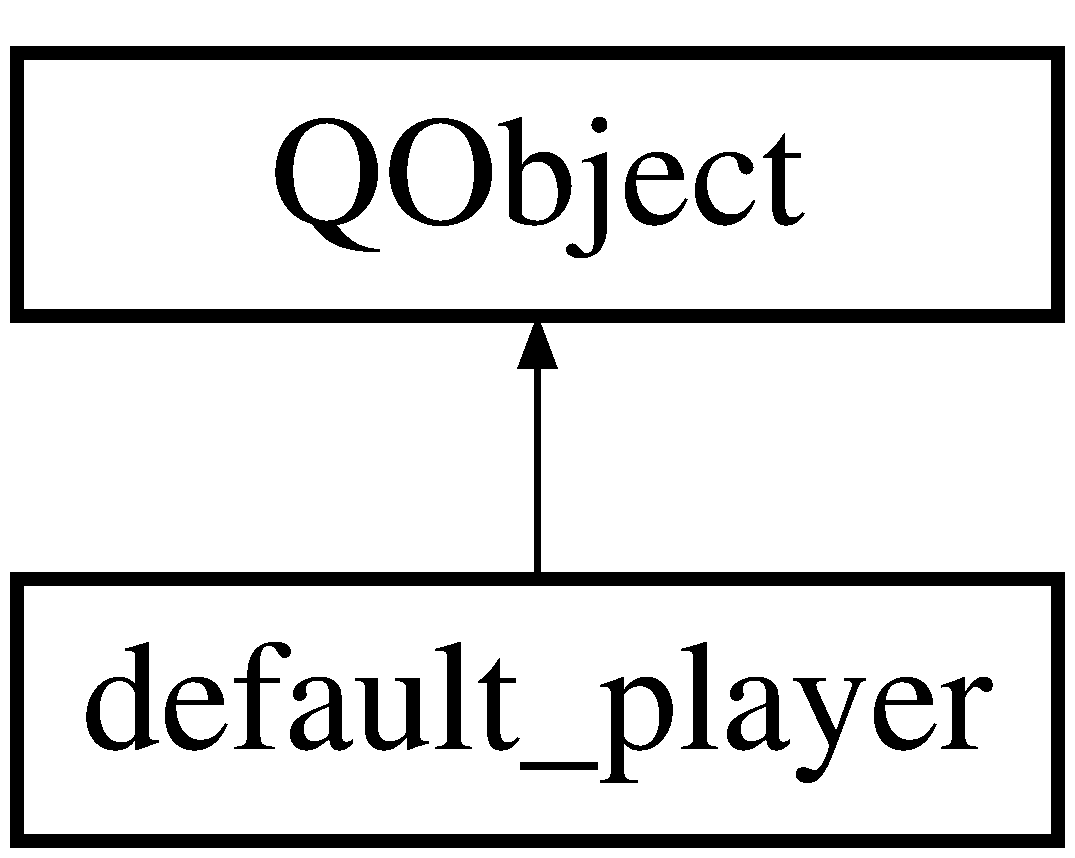
\includegraphics[height=2.000000cm]{classdefault__player}
\end{center}
\end{figure}
\subsection*{Public Member Functions}
\begin{DoxyCompactItemize}
\item 
\hyperlink{classdefault__player_ad6c81fa5385139b5350e4b591844a046}{default\-\_\-player} ()
\begin{DoxyCompactList}\small\item\em Test setup. \end{DoxyCompactList}\end{DoxyCompactItemize}
\subsection*{Private Slots}
\begin{DoxyCompactItemize}
\item 
void \hyperlink{classdefault__player_af05f4c53d52a79c6731621d9488e9f7b}{set\-Name} ()
\begin{DoxyCompactList}\small\item\em Tests changing the player's name. \end{DoxyCompactList}\item 
void \hyperlink{classdefault__player_ad6397356e54526292b855405f410eb22}{add\-Object} ()
\begin{DoxyCompactList}\small\item\em Tests adding an object to the player. \end{DoxyCompactList}\item 
void \hyperlink{classdefault__player_afc294e2e20ad28051ae631ea2cc1e24e}{add\-Objects} ()
\begin{DoxyCompactList}\small\item\em Tests adding an list of objects to the player. \end{DoxyCompactList}\item 
void \hyperlink{classdefault__player_aabdaf180a7edd892d73f8662c780a6d1}{remove\-Object} ()
\begin{DoxyCompactList}\small\item\em Tests removing an object from the player. \end{DoxyCompactList}\item 
void \hyperlink{classdefault__player_a697b3a67efeaa7a58b4a002589496912}{remove\-Object\-\_\-exception\-\_\-keyerror} ()
\begin{DoxyCompactList}\small\item\em Tests removing an object from the player with a \par
wrong key. \end{DoxyCompactList}\item 
void \hyperlink{classdefault__player_ae779c54333e90ea35dab0d387d26e829}{remove\-Object\-\_\-cleanup} ()
\begin{DoxyCompactList}\small\item\em Cleanup after remove test. \end{DoxyCompactList}\item 
void \hyperlink{classdefault__player_a8fed2f00ce871cd36a69c2fa1ae9e92a}{remove\-Objects} ()
\begin{DoxyCompactList}\small\item\em Tests removing a list of objects from the player. \end{DoxyCompactList}\item 
void \hyperlink{classdefault__player_ae749a7881ab40de5bc08c7755beedbc8}{remove\-Objects\-\_\-verify\-\_\-no\-\_\-throw} ()
\begin{DoxyCompactList}\small\item\em Tests removing a list of objects from the player. \end{DoxyCompactList}\item 
void \hyperlink{classdefault__player_afe7db1612cd2af32f26d83a8121bd14c}{remove\-Objects\-\_\-cleanup} ()
\begin{DoxyCompactList}\small\item\em Cleanup after remove test. \end{DoxyCompactList}\item 
void \hyperlink{classdefault__player_af9d8e512b5bf580680a69271e5748afa}{remove\-Object\-\_\-by\-I\-D} ()
\begin{DoxyCompactList}\small\item\em Tests removing an object from the player by I\-D. \end{DoxyCompactList}\item 
void \hyperlink{classdefault__player_afa11b1b1d4fcd5b1e9021b7c4a31cd2c}{remove\-Object\-\_\-by\-I\-D\-\_\-exception} ()
\begin{DoxyCompactList}\small\item\em Tests removing an object from the player by I\-D \par
with the wrong I\-D. \end{DoxyCompactList}\item 
void \hyperlink{classdefault__player_a9b98fbd3caba12fba28349e2495873cc}{remove\-Object\-\_\-by\-I\-D\-\_\-cleanup} ()
\begin{DoxyCompactList}\small\item\em Cleanup after remove test. \end{DoxyCompactList}\item 
void \hyperlink{classdefault__player_a93c22422db2b8fce5164c28fc44f342d}{remove\-Objects\-\_\-by\-I\-D} ()
\begin{DoxyCompactList}\small\item\em Tests removing a list of objects from the player by I\-D. \end{DoxyCompactList}\item 
void \hyperlink{classdefault__player_a4c613b5255994d71ed2343ebdabf4646}{remove\-Objects\-\_\-by\-I\-D\-\_\-cleanup} ()
\begin{DoxyCompactList}\small\item\em Cleanup after remove test. \end{DoxyCompactList}\item 
void \hyperlink{classdefault__player_a37dab33c8c4002f7004b4c9fdcd85e8b}{remove\-Objects\-\_\-by\-I\-D\-\_\-verify\-\_\-no\-\_\-throw} ()
\begin{DoxyCompactList}\small\item\em Tests removing a list of objects from the player by I\-D. \end{DoxyCompactList}\item 
void \hyperlink{classdefault__player_a4bb03f35364f0bf7843fb10095828eeb}{check\-Color} ()
\begin{DoxyCompactList}\small\item\em Tests that a player's color is set up correctly. \end{DoxyCompactList}\item 
void \hyperlink{classdefault__player_aeb1b52f587a7f1593c05783f86eb7b79}{cleanup} ()
\begin{DoxyCompactList}\small\item\em Test cleanup. \end{DoxyCompactList}\end{DoxyCompactItemize}
\subsection*{Private Member Functions}
\begin{DoxyCompactItemize}
\item 
bool \hyperlink{classdefault__player_abc1e0d2a87aa8f8ee30b4ab253b13f31}{vector\-Contains\-Ptr} (std\-::vector$<$ std\-::shared\-\_\-ptr$<$ \hyperlink{classCourse_1_1GameObject}{Course\-::\-Game\-Object} $>$ $>$ vec, std\-::shared\-\_\-ptr$<$ \hyperlink{classCourse_1_1GameObject}{Course\-::\-Game\-Object} $>$ ptr)
\end{DoxyCompactItemize}
\subsection*{Private Attributes}
\begin{DoxyCompactItemize}
\item 
const std\-::string \hyperlink{classdefault__player_a8b90651e56d9ca9aa126384f2890b431}{D\-E\-F\-A\-U\-L\-T\-\_\-\-N\-A\-M\-E} = \char`\"{}Player\char`\"{}
\item 
const std\-::vector\\*
$<$ std\-::shared\-\_\-ptr\\*
$<$ \hyperlink{classCourse_1_1GameObject}{Course\-::\-Game\-Object} $>$ $>$ \hyperlink{classdefault__player_a8e10659ac91777b9f496a0c2e5b1beb9}{B\-L\-A\-N\-K\-\_\-\-O\-B\-J\-E\-C\-T\-S}
\item 
std\-::vector$<$ std\-::shared\-\_\-ptr\\*
$<$ \hyperlink{classCourse_1_1GameObject}{Course\-::\-Game\-Object} $>$ $>$ \hyperlink{classdefault__player_acced0c01b21012d4e52e3326c28633aa}{destroyable\-\_\-objects}
\item 
std\-::unique\-\_\-ptr$<$ \hyperlink{classGame_1_1Player}{Player} $>$ \hyperlink{classdefault__player_a6c7680ccb072390ffcbef8a1b95739c3}{default\-\_\-instance}
\end{DoxyCompactItemize}


\subsection{Detailed Description}
The player\-\_\-tests test the Player\-Base and Player classes. 

\subsection{Constructor \& Destructor Documentation}
\hypertarget{classdefault__player_ad6c81fa5385139b5350e4b591844a046}{\index{default\-\_\-player@{default\-\_\-player}!default\-\_\-player@{default\-\_\-player}}
\index{default\-\_\-player@{default\-\_\-player}!default_player@{default\-\_\-player}}
\subsubsection[{default\-\_\-player}]{\setlength{\rightskip}{0pt plus 5cm}default\-\_\-player\-::default\-\_\-player (
\begin{DoxyParamCaption}
{}
\end{DoxyParamCaption}
)}}\label{classdefault__player_ad6c81fa5385139b5350e4b591844a046}


Test setup. 



\subsection{Member Function Documentation}
\hypertarget{classdefault__player_ad6397356e54526292b855405f410eb22}{\index{default\-\_\-player@{default\-\_\-player}!add\-Object@{add\-Object}}
\index{add\-Object@{add\-Object}!default_player@{default\-\_\-player}}
\subsubsection[{add\-Object}]{\setlength{\rightskip}{0pt plus 5cm}void default\-\_\-player\-::add\-Object (
\begin{DoxyParamCaption}
{}
\end{DoxyParamCaption}
)\hspace{0.3cm}{\ttfamily [private]}, {\ttfamily [slot]}}}\label{classdefault__player_ad6397356e54526292b855405f410eb22}


Tests adding an object to the player. 

\begin{DoxyPostcond}{Postcondition}
Should be added 
\end{DoxyPostcond}
\hypertarget{classdefault__player_afc294e2e20ad28051ae631ea2cc1e24e}{\index{default\-\_\-player@{default\-\_\-player}!add\-Objects@{add\-Objects}}
\index{add\-Objects@{add\-Objects}!default_player@{default\-\_\-player}}
\subsubsection[{add\-Objects}]{\setlength{\rightskip}{0pt plus 5cm}void default\-\_\-player\-::add\-Objects (
\begin{DoxyParamCaption}
{}
\end{DoxyParamCaption}
)\hspace{0.3cm}{\ttfamily [private]}, {\ttfamily [slot]}}}\label{classdefault__player_afc294e2e20ad28051ae631ea2cc1e24e}


Tests adding an list of objects to the player. 

\begin{DoxyPostcond}{Postcondition}
Should be added 
\end{DoxyPostcond}
\hypertarget{classdefault__player_a4bb03f35364f0bf7843fb10095828eeb}{\index{default\-\_\-player@{default\-\_\-player}!check\-Color@{check\-Color}}
\index{check\-Color@{check\-Color}!default_player@{default\-\_\-player}}
\subsubsection[{check\-Color}]{\setlength{\rightskip}{0pt plus 5cm}void default\-\_\-player\-::check\-Color (
\begin{DoxyParamCaption}
{}
\end{DoxyParamCaption}
)\hspace{0.3cm}{\ttfamily [private]}, {\ttfamily [slot]}}}\label{classdefault__player_a4bb03f35364f0bf7843fb10095828eeb}


Tests that a player's color is set up correctly. 

\begin{DoxyPostcond}{Postcondition}
Should be set up correctly 
\end{DoxyPostcond}
\hypertarget{classdefault__player_aeb1b52f587a7f1593c05783f86eb7b79}{\index{default\-\_\-player@{default\-\_\-player}!cleanup@{cleanup}}
\index{cleanup@{cleanup}!default_player@{default\-\_\-player}}
\subsubsection[{cleanup}]{\setlength{\rightskip}{0pt plus 5cm}void default\-\_\-player\-::cleanup (
\begin{DoxyParamCaption}
{}
\end{DoxyParamCaption}
)\hspace{0.3cm}{\ttfamily [private]}, {\ttfamily [slot]}}}\label{classdefault__player_aeb1b52f587a7f1593c05783f86eb7b79}


Test cleanup. 

\hypertarget{classdefault__player_aabdaf180a7edd892d73f8662c780a6d1}{\index{default\-\_\-player@{default\-\_\-player}!remove\-Object@{remove\-Object}}
\index{remove\-Object@{remove\-Object}!default_player@{default\-\_\-player}}
\subsubsection[{remove\-Object}]{\setlength{\rightskip}{0pt plus 5cm}void default\-\_\-player\-::remove\-Object (
\begin{DoxyParamCaption}
{}
\end{DoxyParamCaption}
)\hspace{0.3cm}{\ttfamily [private]}, {\ttfamily [slot]}}}\label{classdefault__player_aabdaf180a7edd892d73f8662c780a6d1}


Tests removing an object from the player. 

\begin{DoxyPostcond}{Postcondition}
Should be removed 
\end{DoxyPostcond}
\hypertarget{classdefault__player_af9d8e512b5bf580680a69271e5748afa}{\index{default\-\_\-player@{default\-\_\-player}!remove\-Object\-\_\-by\-I\-D@{remove\-Object\-\_\-by\-I\-D}}
\index{remove\-Object\-\_\-by\-I\-D@{remove\-Object\-\_\-by\-I\-D}!default_player@{default\-\_\-player}}
\subsubsection[{remove\-Object\-\_\-by\-I\-D}]{\setlength{\rightskip}{0pt plus 5cm}void default\-\_\-player\-::remove\-Object\-\_\-by\-I\-D (
\begin{DoxyParamCaption}
{}
\end{DoxyParamCaption}
)\hspace{0.3cm}{\ttfamily [private]}, {\ttfamily [slot]}}}\label{classdefault__player_af9d8e512b5bf580680a69271e5748afa}


Tests removing an object from the player by I\-D. 

\begin{DoxyPostcond}{Postcondition}
Should be removed 
\end{DoxyPostcond}
\hypertarget{classdefault__player_a9b98fbd3caba12fba28349e2495873cc}{\index{default\-\_\-player@{default\-\_\-player}!remove\-Object\-\_\-by\-I\-D\-\_\-cleanup@{remove\-Object\-\_\-by\-I\-D\-\_\-cleanup}}
\index{remove\-Object\-\_\-by\-I\-D\-\_\-cleanup@{remove\-Object\-\_\-by\-I\-D\-\_\-cleanup}!default_player@{default\-\_\-player}}
\subsubsection[{remove\-Object\-\_\-by\-I\-D\-\_\-cleanup}]{\setlength{\rightskip}{0pt plus 5cm}void default\-\_\-player\-::remove\-Object\-\_\-by\-I\-D\-\_\-cleanup (
\begin{DoxyParamCaption}
{}
\end{DoxyParamCaption}
)\hspace{0.3cm}{\ttfamily [private]}, {\ttfamily [slot]}}}\label{classdefault__player_a9b98fbd3caba12fba28349e2495873cc}


Cleanup after remove test. 

\hypertarget{classdefault__player_afa11b1b1d4fcd5b1e9021b7c4a31cd2c}{\index{default\-\_\-player@{default\-\_\-player}!remove\-Object\-\_\-by\-I\-D\-\_\-exception@{remove\-Object\-\_\-by\-I\-D\-\_\-exception}}
\index{remove\-Object\-\_\-by\-I\-D\-\_\-exception@{remove\-Object\-\_\-by\-I\-D\-\_\-exception}!default_player@{default\-\_\-player}}
\subsubsection[{remove\-Object\-\_\-by\-I\-D\-\_\-exception}]{\setlength{\rightskip}{0pt plus 5cm}void default\-\_\-player\-::remove\-Object\-\_\-by\-I\-D\-\_\-exception (
\begin{DoxyParamCaption}
{}
\end{DoxyParamCaption}
)\hspace{0.3cm}{\ttfamily [private]}, {\ttfamily [slot]}}}\label{classdefault__player_afa11b1b1d4fcd5b1e9021b7c4a31cd2c}


Tests removing an object from the player by I\-D \par
with the wrong I\-D. 

\begin{DoxyPostcond}{Postcondition}
Should throw a Key\-Error exception 
\end{DoxyPostcond}
\hypertarget{classdefault__player_ae779c54333e90ea35dab0d387d26e829}{\index{default\-\_\-player@{default\-\_\-player}!remove\-Object\-\_\-cleanup@{remove\-Object\-\_\-cleanup}}
\index{remove\-Object\-\_\-cleanup@{remove\-Object\-\_\-cleanup}!default_player@{default\-\_\-player}}
\subsubsection[{remove\-Object\-\_\-cleanup}]{\setlength{\rightskip}{0pt plus 5cm}void default\-\_\-player\-::remove\-Object\-\_\-cleanup (
\begin{DoxyParamCaption}
{}
\end{DoxyParamCaption}
)\hspace{0.3cm}{\ttfamily [private]}, {\ttfamily [slot]}}}\label{classdefault__player_ae779c54333e90ea35dab0d387d26e829}


Cleanup after remove test. 

\hypertarget{classdefault__player_a697b3a67efeaa7a58b4a002589496912}{\index{default\-\_\-player@{default\-\_\-player}!remove\-Object\-\_\-exception\-\_\-keyerror@{remove\-Object\-\_\-exception\-\_\-keyerror}}
\index{remove\-Object\-\_\-exception\-\_\-keyerror@{remove\-Object\-\_\-exception\-\_\-keyerror}!default_player@{default\-\_\-player}}
\subsubsection[{remove\-Object\-\_\-exception\-\_\-keyerror}]{\setlength{\rightskip}{0pt plus 5cm}void default\-\_\-player\-::remove\-Object\-\_\-exception\-\_\-keyerror (
\begin{DoxyParamCaption}
{}
\end{DoxyParamCaption}
)\hspace{0.3cm}{\ttfamily [private]}, {\ttfamily [slot]}}}\label{classdefault__player_a697b3a67efeaa7a58b4a002589496912}


Tests removing an object from the player with a \par
wrong key. 

\begin{DoxyPostcond}{Postcondition}
Should throw a Key\-Error exception 
\end{DoxyPostcond}
\hypertarget{classdefault__player_a8fed2f00ce871cd36a69c2fa1ae9e92a}{\index{default\-\_\-player@{default\-\_\-player}!remove\-Objects@{remove\-Objects}}
\index{remove\-Objects@{remove\-Objects}!default_player@{default\-\_\-player}}
\subsubsection[{remove\-Objects}]{\setlength{\rightskip}{0pt plus 5cm}void default\-\_\-player\-::remove\-Objects (
\begin{DoxyParamCaption}
{}
\end{DoxyParamCaption}
)\hspace{0.3cm}{\ttfamily [private]}, {\ttfamily [slot]}}}\label{classdefault__player_a8fed2f00ce871cd36a69c2fa1ae9e92a}


Tests removing a list of objects from the player. 

\begin{DoxyPostcond}{Postcondition}
Should be removed 
\end{DoxyPostcond}
\hypertarget{classdefault__player_a93c22422db2b8fce5164c28fc44f342d}{\index{default\-\_\-player@{default\-\_\-player}!remove\-Objects\-\_\-by\-I\-D@{remove\-Objects\-\_\-by\-I\-D}}
\index{remove\-Objects\-\_\-by\-I\-D@{remove\-Objects\-\_\-by\-I\-D}!default_player@{default\-\_\-player}}
\subsubsection[{remove\-Objects\-\_\-by\-I\-D}]{\setlength{\rightskip}{0pt plus 5cm}void default\-\_\-player\-::remove\-Objects\-\_\-by\-I\-D (
\begin{DoxyParamCaption}
{}
\end{DoxyParamCaption}
)\hspace{0.3cm}{\ttfamily [private]}, {\ttfamily [slot]}}}\label{classdefault__player_a93c22422db2b8fce5164c28fc44f342d}


Tests removing a list of objects from the player by I\-D. 

\begin{DoxyPostcond}{Postcondition}
Should be removed 
\end{DoxyPostcond}
\hypertarget{classdefault__player_a4c613b5255994d71ed2343ebdabf4646}{\index{default\-\_\-player@{default\-\_\-player}!remove\-Objects\-\_\-by\-I\-D\-\_\-cleanup@{remove\-Objects\-\_\-by\-I\-D\-\_\-cleanup}}
\index{remove\-Objects\-\_\-by\-I\-D\-\_\-cleanup@{remove\-Objects\-\_\-by\-I\-D\-\_\-cleanup}!default_player@{default\-\_\-player}}
\subsubsection[{remove\-Objects\-\_\-by\-I\-D\-\_\-cleanup}]{\setlength{\rightskip}{0pt plus 5cm}void default\-\_\-player\-::remove\-Objects\-\_\-by\-I\-D\-\_\-cleanup (
\begin{DoxyParamCaption}
{}
\end{DoxyParamCaption}
)\hspace{0.3cm}{\ttfamily [private]}, {\ttfamily [slot]}}}\label{classdefault__player_a4c613b5255994d71ed2343ebdabf4646}


Cleanup after remove test. 

\hypertarget{classdefault__player_a37dab33c8c4002f7004b4c9fdcd85e8b}{\index{default\-\_\-player@{default\-\_\-player}!remove\-Objects\-\_\-by\-I\-D\-\_\-verify\-\_\-no\-\_\-throw@{remove\-Objects\-\_\-by\-I\-D\-\_\-verify\-\_\-no\-\_\-throw}}
\index{remove\-Objects\-\_\-by\-I\-D\-\_\-verify\-\_\-no\-\_\-throw@{remove\-Objects\-\_\-by\-I\-D\-\_\-verify\-\_\-no\-\_\-throw}!default_player@{default\-\_\-player}}
\subsubsection[{remove\-Objects\-\_\-by\-I\-D\-\_\-verify\-\_\-no\-\_\-throw}]{\setlength{\rightskip}{0pt plus 5cm}void default\-\_\-player\-::remove\-Objects\-\_\-by\-I\-D\-\_\-verify\-\_\-no\-\_\-throw (
\begin{DoxyParamCaption}
{}
\end{DoxyParamCaption}
)\hspace{0.3cm}{\ttfamily [private]}, {\ttfamily [slot]}}}\label{classdefault__player_a37dab33c8c4002f7004b4c9fdcd85e8b}


Tests removing a list of objects from the player by I\-D. 

\begin{DoxyPostcond}{Postcondition}
Should be removed or will not throw an exception 
\end{DoxyPostcond}
\hypertarget{classdefault__player_afe7db1612cd2af32f26d83a8121bd14c}{\index{default\-\_\-player@{default\-\_\-player}!remove\-Objects\-\_\-cleanup@{remove\-Objects\-\_\-cleanup}}
\index{remove\-Objects\-\_\-cleanup@{remove\-Objects\-\_\-cleanup}!default_player@{default\-\_\-player}}
\subsubsection[{remove\-Objects\-\_\-cleanup}]{\setlength{\rightskip}{0pt plus 5cm}void default\-\_\-player\-::remove\-Objects\-\_\-cleanup (
\begin{DoxyParamCaption}
{}
\end{DoxyParamCaption}
)\hspace{0.3cm}{\ttfamily [private]}, {\ttfamily [slot]}}}\label{classdefault__player_afe7db1612cd2af32f26d83a8121bd14c}


Cleanup after remove test. 

\hypertarget{classdefault__player_ae749a7881ab40de5bc08c7755beedbc8}{\index{default\-\_\-player@{default\-\_\-player}!remove\-Objects\-\_\-verify\-\_\-no\-\_\-throw@{remove\-Objects\-\_\-verify\-\_\-no\-\_\-throw}}
\index{remove\-Objects\-\_\-verify\-\_\-no\-\_\-throw@{remove\-Objects\-\_\-verify\-\_\-no\-\_\-throw}!default_player@{default\-\_\-player}}
\subsubsection[{remove\-Objects\-\_\-verify\-\_\-no\-\_\-throw}]{\setlength{\rightskip}{0pt plus 5cm}void default\-\_\-player\-::remove\-Objects\-\_\-verify\-\_\-no\-\_\-throw (
\begin{DoxyParamCaption}
{}
\end{DoxyParamCaption}
)\hspace{0.3cm}{\ttfamily [private]}, {\ttfamily [slot]}}}\label{classdefault__player_ae749a7881ab40de5bc08c7755beedbc8}


Tests removing a list of objects from the player. 

\begin{DoxyPostcond}{Postcondition}
Should be removed or will not throw an exception 
\end{DoxyPostcond}
\hypertarget{classdefault__player_af05f4c53d52a79c6731621d9488e9f7b}{\index{default\-\_\-player@{default\-\_\-player}!set\-Name@{set\-Name}}
\index{set\-Name@{set\-Name}!default_player@{default\-\_\-player}}
\subsubsection[{set\-Name}]{\setlength{\rightskip}{0pt plus 5cm}void default\-\_\-player\-::set\-Name (
\begin{DoxyParamCaption}
{}
\end{DoxyParamCaption}
)\hspace{0.3cm}{\ttfamily [private]}, {\ttfamily [slot]}}}\label{classdefault__player_af05f4c53d52a79c6731621d9488e9f7b}


Tests changing the player's name. 

\begin{DoxyPostcond}{Postcondition}
Should be changed 
\end{DoxyPostcond}
\hypertarget{classdefault__player_abc1e0d2a87aa8f8ee30b4ab253b13f31}{\index{default\-\_\-player@{default\-\_\-player}!vector\-Contains\-Ptr@{vector\-Contains\-Ptr}}
\index{vector\-Contains\-Ptr@{vector\-Contains\-Ptr}!default_player@{default\-\_\-player}}
\subsubsection[{vector\-Contains\-Ptr}]{\setlength{\rightskip}{0pt plus 5cm}bool default\-\_\-player\-::vector\-Contains\-Ptr (
\begin{DoxyParamCaption}
\item[{std\-::vector$<$ std\-::shared\-\_\-ptr$<$ {\bf Course\-::\-Game\-Object} $>$ $>$}]{vec, }
\item[{std\-::shared\-\_\-ptr$<$ {\bf Course\-::\-Game\-Object} $>$}]{ptr}
\end{DoxyParamCaption}
)\hspace{0.3cm}{\ttfamily [private]}}}\label{classdefault__player_abc1e0d2a87aa8f8ee30b4ab253b13f31}


\subsection{Member Data Documentation}
\hypertarget{classdefault__player_a8e10659ac91777b9f496a0c2e5b1beb9}{\index{default\-\_\-player@{default\-\_\-player}!B\-L\-A\-N\-K\-\_\-\-O\-B\-J\-E\-C\-T\-S@{B\-L\-A\-N\-K\-\_\-\-O\-B\-J\-E\-C\-T\-S}}
\index{B\-L\-A\-N\-K\-\_\-\-O\-B\-J\-E\-C\-T\-S@{B\-L\-A\-N\-K\-\_\-\-O\-B\-J\-E\-C\-T\-S}!default_player@{default\-\_\-player}}
\subsubsection[{B\-L\-A\-N\-K\-\_\-\-O\-B\-J\-E\-C\-T\-S}]{\setlength{\rightskip}{0pt plus 5cm}const std\-::vector$<$std\-::shared\-\_\-ptr$<${\bf Course\-::\-Game\-Object}$>$ $>$ default\-\_\-player\-::\-B\-L\-A\-N\-K\-\_\-\-O\-B\-J\-E\-C\-T\-S\hspace{0.3cm}{\ttfamily [private]}}}\label{classdefault__player_a8e10659ac91777b9f496a0c2e5b1beb9}
{\bfseries Initial value\-:}
\begin{DoxyCode}
= \{
        std::make\_shared<Course::GameObject>(),
        std::make\_shared<Course::GameObject>(),
        std::make\_shared<Course::GameObject>(),
        std::make\_shared<Course::GameObject>(),
        std::make\_shared<Course::GameObject>(),

    \}
\end{DoxyCode}
\hypertarget{classdefault__player_a6c7680ccb072390ffcbef8a1b95739c3}{\index{default\-\_\-player@{default\-\_\-player}!default\-\_\-instance@{default\-\_\-instance}}
\index{default\-\_\-instance@{default\-\_\-instance}!default_player@{default\-\_\-player}}
\subsubsection[{default\-\_\-instance}]{\setlength{\rightskip}{0pt plus 5cm}std\-::unique\-\_\-ptr$<${\bf Player}$>$ default\-\_\-player\-::default\-\_\-instance\hspace{0.3cm}{\ttfamily [private]}}}\label{classdefault__player_a6c7680ccb072390ffcbef8a1b95739c3}
\hypertarget{classdefault__player_a8b90651e56d9ca9aa126384f2890b431}{\index{default\-\_\-player@{default\-\_\-player}!D\-E\-F\-A\-U\-L\-T\-\_\-\-N\-A\-M\-E@{D\-E\-F\-A\-U\-L\-T\-\_\-\-N\-A\-M\-E}}
\index{D\-E\-F\-A\-U\-L\-T\-\_\-\-N\-A\-M\-E@{D\-E\-F\-A\-U\-L\-T\-\_\-\-N\-A\-M\-E}!default_player@{default\-\_\-player}}
\subsubsection[{D\-E\-F\-A\-U\-L\-T\-\_\-\-N\-A\-M\-E}]{\setlength{\rightskip}{0pt plus 5cm}const std\-::string default\-\_\-player\-::\-D\-E\-F\-A\-U\-L\-T\-\_\-\-N\-A\-M\-E = \char`\"{}Player\char`\"{}\hspace{0.3cm}{\ttfamily [private]}}}\label{classdefault__player_a8b90651e56d9ca9aa126384f2890b431}
\hypertarget{classdefault__player_acced0c01b21012d4e52e3326c28633aa}{\index{default\-\_\-player@{default\-\_\-player}!destroyable\-\_\-objects@{destroyable\-\_\-objects}}
\index{destroyable\-\_\-objects@{destroyable\-\_\-objects}!default_player@{default\-\_\-player}}
\subsubsection[{destroyable\-\_\-objects}]{\setlength{\rightskip}{0pt plus 5cm}std\-::vector$<$std\-::shared\-\_\-ptr$<${\bf Course\-::\-Game\-Object}$>$ $>$ default\-\_\-player\-::destroyable\-\_\-objects\hspace{0.3cm}{\ttfamily [private]}}}\label{classdefault__player_acced0c01b21012d4e52e3326c28633aa}


The documentation for this class was generated from the following file\-:\begin{DoxyCompactItemize}
\item 
Unit\-Tests/player\-\_\-tests/\hyperlink{tst__default__player_8cpp}{tst\-\_\-default\-\_\-player.\-cpp}\end{DoxyCompactItemize}

\hypertarget{classdefault__playerbase}{\section{default\-\_\-playerbase Class Reference}
\label{classdefault__playerbase}\index{default\-\_\-playerbase@{default\-\_\-playerbase}}
}
Inheritance diagram for default\-\_\-playerbase\-:\begin{figure}[H]
\begin{center}
\leavevmode
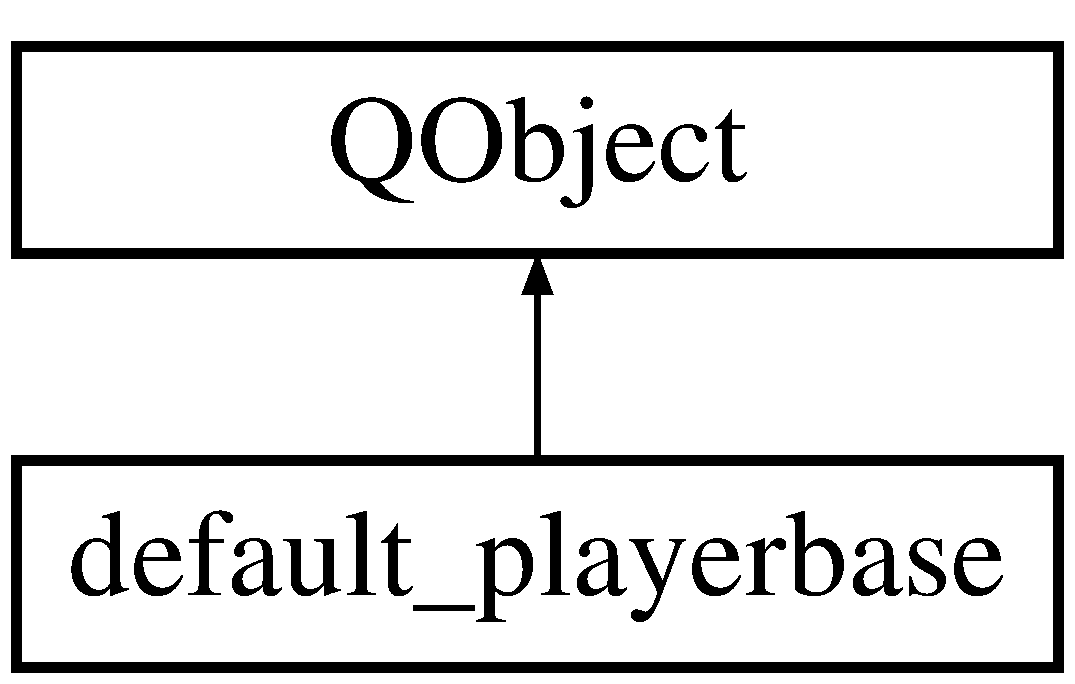
\includegraphics[height=2.000000cm]{classdefault__playerbase}
\end{center}
\end{figure}
\subsection*{Public Member Functions}
\begin{DoxyCompactItemize}
\item 
\hyperlink{classdefault__playerbase_ad96867ee8989920a4a72556b0a3441ec}{default\-\_\-playerbase} ()
\item 
\hyperlink{classdefault__playerbase_a621f3dd0b418ebea179a748e7e875d5d}{$\sim$default\-\_\-playerbase} ()
\end{DoxyCompactItemize}
\subsection*{Private Slots}
\begin{DoxyCompactItemize}
\item 
void \hyperlink{classdefault__playerbase_aeca851e45b82a35e314594e9fa895447}{set\-Name} ()
\item 
void \hyperlink{classdefault__playerbase_ad1f183df28852e74c155f49db5b17702}{add\-Object} ()
\item 
void \hyperlink{classdefault__playerbase_ab4a6152ea15d7fba3a305cde06563250}{add\-Objects} ()
\item 
void \hyperlink{classdefault__playerbase_aee868856c989eaba1fba591024921711}{remove\-Object} ()
\item 
void \hyperlink{classdefault__playerbase_ad8ee69e49d61514bbfb6441165045288}{remove\-Object\-\_\-exception\-\_\-keyerror} ()
\item 
void \hyperlink{classdefault__playerbase_a0d762ce7d0fcfbbbbe7da4764832d3d7}{remove\-Object\-\_\-cleanup} ()
\item 
void \hyperlink{classdefault__playerbase_ab0435d999f7f24a39b13a753a28b57e5}{remove\-Objects} ()
\item 
void \hyperlink{classdefault__playerbase_ac76a8293414dee2a11baa4059aabd707}{remove\-Objects\-\_\-verify\-\_\-no\-\_\-throw} ()
\item 
void \hyperlink{classdefault__playerbase_afcc8ecbf9f084799b07812485165cca3}{remove\-Objects\-\_\-cleanup} ()
\item 
void \hyperlink{classdefault__playerbase_a1b1dac346d1ad3f38f09c956763ebda3}{remove\-Object\-\_\-by\-I\-D} ()
\item 
void \hyperlink{classdefault__playerbase_a98744fc4c97cb7d468d432baf99da59a}{remove\-Object\-\_\-by\-I\-D\-\_\-exception} ()
\item 
void \hyperlink{classdefault__playerbase_aae868dda496dafc8c28267c08c03a9d6}{remove\-Object\-\_\-by\-I\-D\-\_\-cleanup} ()
\item 
void \hyperlink{classdefault__playerbase_a87b8f296fefa5731303dc4e1c9a1f3c9}{remove\-Objects\-\_\-by\-I\-D} ()
\item 
void \hyperlink{classdefault__playerbase_a4b6b6efae3c2c4fc9d27ac382f25cd61}{remove\-Objects\-\_\-by\-I\-D\-\_\-cleanup} ()
\item 
void \hyperlink{classdefault__playerbase_aed32848900592ff043e0e9583e59f27f}{remove\-Objects\-\_\-by\-I\-D\-\_\-verify\-\_\-no\-\_\-throw} ()
\item 
void \hyperlink{classdefault__playerbase_a8a5165112d5927d48e7f213446bb63a0}{cleanup} ()
\end{DoxyCompactItemize}
\subsection*{Private Member Functions}
\begin{DoxyCompactItemize}
\item 
bool \hyperlink{classdefault__playerbase_aa4531b2048b87ed76dbac6211e6e29a3}{vector\-Contains\-Ptr} (std\-::vector$<$ std\-::shared\-\_\-ptr$<$ \hyperlink{classCourse_1_1GameObject}{Game\-Object} $>$ $>$ vec, std\-::shared\-\_\-ptr$<$ \hyperlink{classCourse_1_1GameObject}{Game\-Object} $>$ ptr)
\end{DoxyCompactItemize}
\subsection*{Private Attributes}
\begin{DoxyCompactItemize}
\item 
const std\-::string \hyperlink{classdefault__playerbase_a765fd2269477fdbc4e9089fe6c289736}{D\-E\-F\-A\-U\-L\-T\-\_\-\-N\-A\-M\-E} = \char`\"{}Player\char`\"{}
\item 
const std\-::vector\\*
$<$ std\-::shared\-\_\-ptr$<$ \hyperlink{classCourse_1_1GameObject}{Game\-Object} $>$ $>$ \hyperlink{classdefault__playerbase_a06e9be69d4ee621b71bfb2ab8b02aaa5}{B\-L\-A\-N\-K\-\_\-\-O\-B\-J\-E\-C\-T\-S}
\item 
std\-::vector$<$ std\-::shared\-\_\-ptr\\*
$<$ \hyperlink{classCourse_1_1GameObject}{Game\-Object} $>$ $>$ \hyperlink{classdefault__playerbase_a2d96091c3d07febe37760c9925ec6e1a}{destroyable\-\_\-objects}
\item 
std\-::unique\-\_\-ptr$<$ \hyperlink{classCourse_1_1PlayerBase}{Player\-Base} $>$ \hyperlink{classdefault__playerbase_a703e1d8144130378036db93a04158bf1}{default\-\_\-instance}
\end{DoxyCompactItemize}


\subsection{Constructor \& Destructor Documentation}
\hypertarget{classdefault__playerbase_ad96867ee8989920a4a72556b0a3441ec}{\index{default\-\_\-playerbase@{default\-\_\-playerbase}!default\-\_\-playerbase@{default\-\_\-playerbase}}
\index{default\-\_\-playerbase@{default\-\_\-playerbase}!default_playerbase@{default\-\_\-playerbase}}
\subsubsection[{default\-\_\-playerbase}]{\setlength{\rightskip}{0pt plus 5cm}default\-\_\-playerbase\-::default\-\_\-playerbase (
\begin{DoxyParamCaption}
{}
\end{DoxyParamCaption}
)}}\label{classdefault__playerbase_ad96867ee8989920a4a72556b0a3441ec}
\hypertarget{classdefault__playerbase_a621f3dd0b418ebea179a748e7e875d5d}{\index{default\-\_\-playerbase@{default\-\_\-playerbase}!$\sim$default\-\_\-playerbase@{$\sim$default\-\_\-playerbase}}
\index{$\sim$default\-\_\-playerbase@{$\sim$default\-\_\-playerbase}!default_playerbase@{default\-\_\-playerbase}}
\subsubsection[{$\sim$default\-\_\-playerbase}]{\setlength{\rightskip}{0pt plus 5cm}default\-\_\-playerbase\-::$\sim$default\-\_\-playerbase (
\begin{DoxyParamCaption}
{}
\end{DoxyParamCaption}
)}}\label{classdefault__playerbase_a621f3dd0b418ebea179a748e7e875d5d}


\subsection{Member Function Documentation}
\hypertarget{classdefault__playerbase_ad1f183df28852e74c155f49db5b17702}{\index{default\-\_\-playerbase@{default\-\_\-playerbase}!add\-Object@{add\-Object}}
\index{add\-Object@{add\-Object}!default_playerbase@{default\-\_\-playerbase}}
\subsubsection[{add\-Object}]{\setlength{\rightskip}{0pt plus 5cm}void default\-\_\-playerbase\-::add\-Object (
\begin{DoxyParamCaption}
{}
\end{DoxyParamCaption}
)\hspace{0.3cm}{\ttfamily [private]}, {\ttfamily [slot]}}}\label{classdefault__playerbase_ad1f183df28852e74c155f49db5b17702}
\hypertarget{classdefault__playerbase_ab4a6152ea15d7fba3a305cde06563250}{\index{default\-\_\-playerbase@{default\-\_\-playerbase}!add\-Objects@{add\-Objects}}
\index{add\-Objects@{add\-Objects}!default_playerbase@{default\-\_\-playerbase}}
\subsubsection[{add\-Objects}]{\setlength{\rightskip}{0pt plus 5cm}void default\-\_\-playerbase\-::add\-Objects (
\begin{DoxyParamCaption}
{}
\end{DoxyParamCaption}
)\hspace{0.3cm}{\ttfamily [private]}, {\ttfamily [slot]}}}\label{classdefault__playerbase_ab4a6152ea15d7fba3a305cde06563250}
\hypertarget{classdefault__playerbase_a8a5165112d5927d48e7f213446bb63a0}{\index{default\-\_\-playerbase@{default\-\_\-playerbase}!cleanup@{cleanup}}
\index{cleanup@{cleanup}!default_playerbase@{default\-\_\-playerbase}}
\subsubsection[{cleanup}]{\setlength{\rightskip}{0pt plus 5cm}void default\-\_\-playerbase\-::cleanup (
\begin{DoxyParamCaption}
{}
\end{DoxyParamCaption}
)\hspace{0.3cm}{\ttfamily [private]}, {\ttfamily [slot]}}}\label{classdefault__playerbase_a8a5165112d5927d48e7f213446bb63a0}
\hypertarget{classdefault__playerbase_aee868856c989eaba1fba591024921711}{\index{default\-\_\-playerbase@{default\-\_\-playerbase}!remove\-Object@{remove\-Object}}
\index{remove\-Object@{remove\-Object}!default_playerbase@{default\-\_\-playerbase}}
\subsubsection[{remove\-Object}]{\setlength{\rightskip}{0pt plus 5cm}void default\-\_\-playerbase\-::remove\-Object (
\begin{DoxyParamCaption}
{}
\end{DoxyParamCaption}
)\hspace{0.3cm}{\ttfamily [private]}, {\ttfamily [slot]}}}\label{classdefault__playerbase_aee868856c989eaba1fba591024921711}
\hypertarget{classdefault__playerbase_a1b1dac346d1ad3f38f09c956763ebda3}{\index{default\-\_\-playerbase@{default\-\_\-playerbase}!remove\-Object\-\_\-by\-I\-D@{remove\-Object\-\_\-by\-I\-D}}
\index{remove\-Object\-\_\-by\-I\-D@{remove\-Object\-\_\-by\-I\-D}!default_playerbase@{default\-\_\-playerbase}}
\subsubsection[{remove\-Object\-\_\-by\-I\-D}]{\setlength{\rightskip}{0pt plus 5cm}void default\-\_\-playerbase\-::remove\-Object\-\_\-by\-I\-D (
\begin{DoxyParamCaption}
{}
\end{DoxyParamCaption}
)\hspace{0.3cm}{\ttfamily [private]}, {\ttfamily [slot]}}}\label{classdefault__playerbase_a1b1dac346d1ad3f38f09c956763ebda3}
\hypertarget{classdefault__playerbase_aae868dda496dafc8c28267c08c03a9d6}{\index{default\-\_\-playerbase@{default\-\_\-playerbase}!remove\-Object\-\_\-by\-I\-D\-\_\-cleanup@{remove\-Object\-\_\-by\-I\-D\-\_\-cleanup}}
\index{remove\-Object\-\_\-by\-I\-D\-\_\-cleanup@{remove\-Object\-\_\-by\-I\-D\-\_\-cleanup}!default_playerbase@{default\-\_\-playerbase}}
\subsubsection[{remove\-Object\-\_\-by\-I\-D\-\_\-cleanup}]{\setlength{\rightskip}{0pt plus 5cm}void default\-\_\-playerbase\-::remove\-Object\-\_\-by\-I\-D\-\_\-cleanup (
\begin{DoxyParamCaption}
{}
\end{DoxyParamCaption}
)\hspace{0.3cm}{\ttfamily [private]}, {\ttfamily [slot]}}}\label{classdefault__playerbase_aae868dda496dafc8c28267c08c03a9d6}
\hypertarget{classdefault__playerbase_a98744fc4c97cb7d468d432baf99da59a}{\index{default\-\_\-playerbase@{default\-\_\-playerbase}!remove\-Object\-\_\-by\-I\-D\-\_\-exception@{remove\-Object\-\_\-by\-I\-D\-\_\-exception}}
\index{remove\-Object\-\_\-by\-I\-D\-\_\-exception@{remove\-Object\-\_\-by\-I\-D\-\_\-exception}!default_playerbase@{default\-\_\-playerbase}}
\subsubsection[{remove\-Object\-\_\-by\-I\-D\-\_\-exception}]{\setlength{\rightskip}{0pt plus 5cm}void default\-\_\-playerbase\-::remove\-Object\-\_\-by\-I\-D\-\_\-exception (
\begin{DoxyParamCaption}
{}
\end{DoxyParamCaption}
)\hspace{0.3cm}{\ttfamily [private]}, {\ttfamily [slot]}}}\label{classdefault__playerbase_a98744fc4c97cb7d468d432baf99da59a}
\hypertarget{classdefault__playerbase_a0d762ce7d0fcfbbbbe7da4764832d3d7}{\index{default\-\_\-playerbase@{default\-\_\-playerbase}!remove\-Object\-\_\-cleanup@{remove\-Object\-\_\-cleanup}}
\index{remove\-Object\-\_\-cleanup@{remove\-Object\-\_\-cleanup}!default_playerbase@{default\-\_\-playerbase}}
\subsubsection[{remove\-Object\-\_\-cleanup}]{\setlength{\rightskip}{0pt plus 5cm}void default\-\_\-playerbase\-::remove\-Object\-\_\-cleanup (
\begin{DoxyParamCaption}
{}
\end{DoxyParamCaption}
)\hspace{0.3cm}{\ttfamily [private]}, {\ttfamily [slot]}}}\label{classdefault__playerbase_a0d762ce7d0fcfbbbbe7da4764832d3d7}
\hypertarget{classdefault__playerbase_ad8ee69e49d61514bbfb6441165045288}{\index{default\-\_\-playerbase@{default\-\_\-playerbase}!remove\-Object\-\_\-exception\-\_\-keyerror@{remove\-Object\-\_\-exception\-\_\-keyerror}}
\index{remove\-Object\-\_\-exception\-\_\-keyerror@{remove\-Object\-\_\-exception\-\_\-keyerror}!default_playerbase@{default\-\_\-playerbase}}
\subsubsection[{remove\-Object\-\_\-exception\-\_\-keyerror}]{\setlength{\rightskip}{0pt plus 5cm}void default\-\_\-playerbase\-::remove\-Object\-\_\-exception\-\_\-keyerror (
\begin{DoxyParamCaption}
{}
\end{DoxyParamCaption}
)\hspace{0.3cm}{\ttfamily [private]}, {\ttfamily [slot]}}}\label{classdefault__playerbase_ad8ee69e49d61514bbfb6441165045288}
\hypertarget{classdefault__playerbase_ab0435d999f7f24a39b13a753a28b57e5}{\index{default\-\_\-playerbase@{default\-\_\-playerbase}!remove\-Objects@{remove\-Objects}}
\index{remove\-Objects@{remove\-Objects}!default_playerbase@{default\-\_\-playerbase}}
\subsubsection[{remove\-Objects}]{\setlength{\rightskip}{0pt plus 5cm}void default\-\_\-playerbase\-::remove\-Objects (
\begin{DoxyParamCaption}
{}
\end{DoxyParamCaption}
)\hspace{0.3cm}{\ttfamily [private]}, {\ttfamily [slot]}}}\label{classdefault__playerbase_ab0435d999f7f24a39b13a753a28b57e5}
\hypertarget{classdefault__playerbase_a87b8f296fefa5731303dc4e1c9a1f3c9}{\index{default\-\_\-playerbase@{default\-\_\-playerbase}!remove\-Objects\-\_\-by\-I\-D@{remove\-Objects\-\_\-by\-I\-D}}
\index{remove\-Objects\-\_\-by\-I\-D@{remove\-Objects\-\_\-by\-I\-D}!default_playerbase@{default\-\_\-playerbase}}
\subsubsection[{remove\-Objects\-\_\-by\-I\-D}]{\setlength{\rightskip}{0pt plus 5cm}void default\-\_\-playerbase\-::remove\-Objects\-\_\-by\-I\-D (
\begin{DoxyParamCaption}
{}
\end{DoxyParamCaption}
)\hspace{0.3cm}{\ttfamily [private]}, {\ttfamily [slot]}}}\label{classdefault__playerbase_a87b8f296fefa5731303dc4e1c9a1f3c9}
\hypertarget{classdefault__playerbase_a4b6b6efae3c2c4fc9d27ac382f25cd61}{\index{default\-\_\-playerbase@{default\-\_\-playerbase}!remove\-Objects\-\_\-by\-I\-D\-\_\-cleanup@{remove\-Objects\-\_\-by\-I\-D\-\_\-cleanup}}
\index{remove\-Objects\-\_\-by\-I\-D\-\_\-cleanup@{remove\-Objects\-\_\-by\-I\-D\-\_\-cleanup}!default_playerbase@{default\-\_\-playerbase}}
\subsubsection[{remove\-Objects\-\_\-by\-I\-D\-\_\-cleanup}]{\setlength{\rightskip}{0pt plus 5cm}void default\-\_\-playerbase\-::remove\-Objects\-\_\-by\-I\-D\-\_\-cleanup (
\begin{DoxyParamCaption}
{}
\end{DoxyParamCaption}
)\hspace{0.3cm}{\ttfamily [private]}, {\ttfamily [slot]}}}\label{classdefault__playerbase_a4b6b6efae3c2c4fc9d27ac382f25cd61}
\hypertarget{classdefault__playerbase_aed32848900592ff043e0e9583e59f27f}{\index{default\-\_\-playerbase@{default\-\_\-playerbase}!remove\-Objects\-\_\-by\-I\-D\-\_\-verify\-\_\-no\-\_\-throw@{remove\-Objects\-\_\-by\-I\-D\-\_\-verify\-\_\-no\-\_\-throw}}
\index{remove\-Objects\-\_\-by\-I\-D\-\_\-verify\-\_\-no\-\_\-throw@{remove\-Objects\-\_\-by\-I\-D\-\_\-verify\-\_\-no\-\_\-throw}!default_playerbase@{default\-\_\-playerbase}}
\subsubsection[{remove\-Objects\-\_\-by\-I\-D\-\_\-verify\-\_\-no\-\_\-throw}]{\setlength{\rightskip}{0pt plus 5cm}void default\-\_\-playerbase\-::remove\-Objects\-\_\-by\-I\-D\-\_\-verify\-\_\-no\-\_\-throw (
\begin{DoxyParamCaption}
{}
\end{DoxyParamCaption}
)\hspace{0.3cm}{\ttfamily [private]}, {\ttfamily [slot]}}}\label{classdefault__playerbase_aed32848900592ff043e0e9583e59f27f}
\hypertarget{classdefault__playerbase_afcc8ecbf9f084799b07812485165cca3}{\index{default\-\_\-playerbase@{default\-\_\-playerbase}!remove\-Objects\-\_\-cleanup@{remove\-Objects\-\_\-cleanup}}
\index{remove\-Objects\-\_\-cleanup@{remove\-Objects\-\_\-cleanup}!default_playerbase@{default\-\_\-playerbase}}
\subsubsection[{remove\-Objects\-\_\-cleanup}]{\setlength{\rightskip}{0pt plus 5cm}void default\-\_\-playerbase\-::remove\-Objects\-\_\-cleanup (
\begin{DoxyParamCaption}
{}
\end{DoxyParamCaption}
)\hspace{0.3cm}{\ttfamily [private]}, {\ttfamily [slot]}}}\label{classdefault__playerbase_afcc8ecbf9f084799b07812485165cca3}
\hypertarget{classdefault__playerbase_ac76a8293414dee2a11baa4059aabd707}{\index{default\-\_\-playerbase@{default\-\_\-playerbase}!remove\-Objects\-\_\-verify\-\_\-no\-\_\-throw@{remove\-Objects\-\_\-verify\-\_\-no\-\_\-throw}}
\index{remove\-Objects\-\_\-verify\-\_\-no\-\_\-throw@{remove\-Objects\-\_\-verify\-\_\-no\-\_\-throw}!default_playerbase@{default\-\_\-playerbase}}
\subsubsection[{remove\-Objects\-\_\-verify\-\_\-no\-\_\-throw}]{\setlength{\rightskip}{0pt plus 5cm}void default\-\_\-playerbase\-::remove\-Objects\-\_\-verify\-\_\-no\-\_\-throw (
\begin{DoxyParamCaption}
{}
\end{DoxyParamCaption}
)\hspace{0.3cm}{\ttfamily [private]}, {\ttfamily [slot]}}}\label{classdefault__playerbase_ac76a8293414dee2a11baa4059aabd707}
\hypertarget{classdefault__playerbase_aeca851e45b82a35e314594e9fa895447}{\index{default\-\_\-playerbase@{default\-\_\-playerbase}!set\-Name@{set\-Name}}
\index{set\-Name@{set\-Name}!default_playerbase@{default\-\_\-playerbase}}
\subsubsection[{set\-Name}]{\setlength{\rightskip}{0pt plus 5cm}void default\-\_\-playerbase\-::set\-Name (
\begin{DoxyParamCaption}
{}
\end{DoxyParamCaption}
)\hspace{0.3cm}{\ttfamily [private]}, {\ttfamily [slot]}}}\label{classdefault__playerbase_aeca851e45b82a35e314594e9fa895447}
\hypertarget{classdefault__playerbase_aa4531b2048b87ed76dbac6211e6e29a3}{\index{default\-\_\-playerbase@{default\-\_\-playerbase}!vector\-Contains\-Ptr@{vector\-Contains\-Ptr}}
\index{vector\-Contains\-Ptr@{vector\-Contains\-Ptr}!default_playerbase@{default\-\_\-playerbase}}
\subsubsection[{vector\-Contains\-Ptr}]{\setlength{\rightskip}{0pt plus 5cm}bool default\-\_\-playerbase\-::vector\-Contains\-Ptr (
\begin{DoxyParamCaption}
\item[{std\-::vector$<$ std\-::shared\-\_\-ptr$<$ {\bf Game\-Object} $>$ $>$}]{vec, }
\item[{std\-::shared\-\_\-ptr$<$ {\bf Game\-Object} $>$}]{ptr}
\end{DoxyParamCaption}
)\hspace{0.3cm}{\ttfamily [private]}}}\label{classdefault__playerbase_aa4531b2048b87ed76dbac6211e6e29a3}


\subsection{Member Data Documentation}
\hypertarget{classdefault__playerbase_a06e9be69d4ee621b71bfb2ab8b02aaa5}{\index{default\-\_\-playerbase@{default\-\_\-playerbase}!B\-L\-A\-N\-K\-\_\-\-O\-B\-J\-E\-C\-T\-S@{B\-L\-A\-N\-K\-\_\-\-O\-B\-J\-E\-C\-T\-S}}
\index{B\-L\-A\-N\-K\-\_\-\-O\-B\-J\-E\-C\-T\-S@{B\-L\-A\-N\-K\-\_\-\-O\-B\-J\-E\-C\-T\-S}!default_playerbase@{default\-\_\-playerbase}}
\subsubsection[{B\-L\-A\-N\-K\-\_\-\-O\-B\-J\-E\-C\-T\-S}]{\setlength{\rightskip}{0pt plus 5cm}const std\-::vector$<$std\-::shared\-\_\-ptr$<${\bf Game\-Object}$>$ $>$ default\-\_\-playerbase\-::\-B\-L\-A\-N\-K\-\_\-\-O\-B\-J\-E\-C\-T\-S\hspace{0.3cm}{\ttfamily [private]}}}\label{classdefault__playerbase_a06e9be69d4ee621b71bfb2ab8b02aaa5}
{\bfseries Initial value\-:}
\begin{DoxyCode}
= \{
        std::make\_shared<GameObject>(),
        std::make\_shared<GameObject>(),
        std::make\_shared<GameObject>(),
        std::make\_shared<GameObject>(),
        std::make\_shared<GameObject>(),

    \}
\end{DoxyCode}
\hypertarget{classdefault__playerbase_a703e1d8144130378036db93a04158bf1}{\index{default\-\_\-playerbase@{default\-\_\-playerbase}!default\-\_\-instance@{default\-\_\-instance}}
\index{default\-\_\-instance@{default\-\_\-instance}!default_playerbase@{default\-\_\-playerbase}}
\subsubsection[{default\-\_\-instance}]{\setlength{\rightskip}{0pt plus 5cm}std\-::unique\-\_\-ptr$<${\bf Player\-Base}$>$ default\-\_\-playerbase\-::default\-\_\-instance\hspace{0.3cm}{\ttfamily [private]}}}\label{classdefault__playerbase_a703e1d8144130378036db93a04158bf1}
\hypertarget{classdefault__playerbase_a765fd2269477fdbc4e9089fe6c289736}{\index{default\-\_\-playerbase@{default\-\_\-playerbase}!D\-E\-F\-A\-U\-L\-T\-\_\-\-N\-A\-M\-E@{D\-E\-F\-A\-U\-L\-T\-\_\-\-N\-A\-M\-E}}
\index{D\-E\-F\-A\-U\-L\-T\-\_\-\-N\-A\-M\-E@{D\-E\-F\-A\-U\-L\-T\-\_\-\-N\-A\-M\-E}!default_playerbase@{default\-\_\-playerbase}}
\subsubsection[{D\-E\-F\-A\-U\-L\-T\-\_\-\-N\-A\-M\-E}]{\setlength{\rightskip}{0pt plus 5cm}const std\-::string default\-\_\-playerbase\-::\-D\-E\-F\-A\-U\-L\-T\-\_\-\-N\-A\-M\-E = \char`\"{}Player\char`\"{}\hspace{0.3cm}{\ttfamily [private]}}}\label{classdefault__playerbase_a765fd2269477fdbc4e9089fe6c289736}
\hypertarget{classdefault__playerbase_a2d96091c3d07febe37760c9925ec6e1a}{\index{default\-\_\-playerbase@{default\-\_\-playerbase}!destroyable\-\_\-objects@{destroyable\-\_\-objects}}
\index{destroyable\-\_\-objects@{destroyable\-\_\-objects}!default_playerbase@{default\-\_\-playerbase}}
\subsubsection[{destroyable\-\_\-objects}]{\setlength{\rightskip}{0pt plus 5cm}std\-::vector$<$std\-::shared\-\_\-ptr$<${\bf Game\-Object}$>$ $>$ default\-\_\-playerbase\-::destroyable\-\_\-objects\hspace{0.3cm}{\ttfamily [private]}}}\label{classdefault__playerbase_a2d96091c3d07febe37760c9925ec6e1a}


The documentation for this class was generated from the following file\-:\begin{DoxyCompactItemize}
\item 
Course/\-Unit\-Tests/playerbase\-\_\-tests/\hyperlink{tst__default__playerbase_8cpp}{tst\-\_\-default\-\_\-playerbase.\-cpp}\end{DoxyCompactItemize}

\hypertarget{classdefault__test}{\section{default\-\_\-test Class Reference}
\label{classdefault__test}\index{default\-\_\-test@{default\-\_\-test}}
}
Inheritance diagram for default\-\_\-test\-:\begin{figure}[H]
\begin{center}
\leavevmode
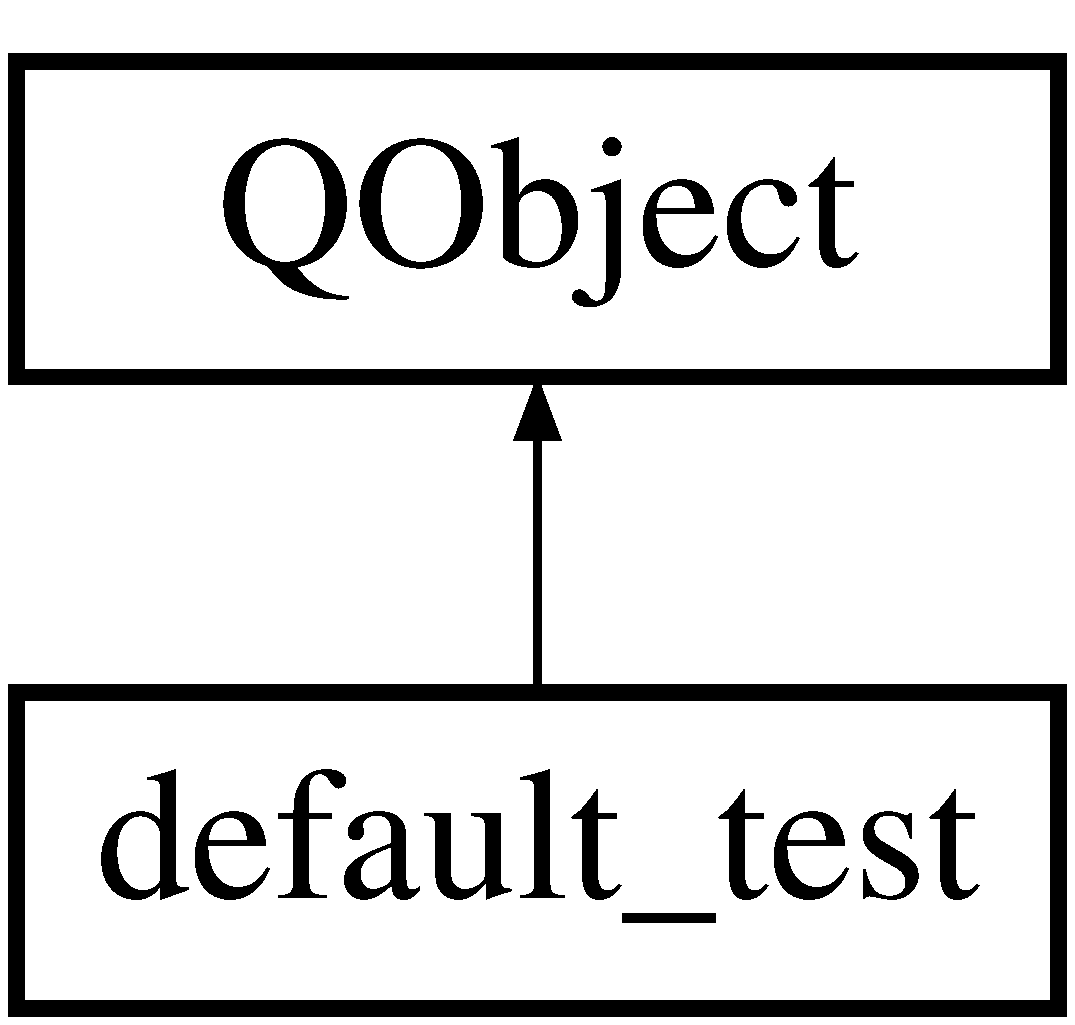
\includegraphics[height=2.000000cm]{classdefault__test}
\end{center}
\end{figure}
\subsection*{Public Member Functions}
\begin{DoxyCompactItemize}
\item 
\hyperlink{classdefault__test_adc43e1333543986f2b1cea153e55e64e}{default\-\_\-test} ()
\end{DoxyCompactItemize}
\subsection*{Private Slots}
\begin{DoxyCompactItemize}
\item 
void \hyperlink{classdefault__test_a4529264e0eb70a16261b0005a28185b8}{test\-\_\-can\-Be\-Placed\-On\-Tile\-\_\-same\-\_\-owner} ()
\item 
void \hyperlink{classdefault__test_a936c70b0c81a6d5e6fb3ffe1e9a49f57}{test\-\_\-can\-Be\-Placed\-On\-Tile\-\_\-ownerconflict} ()
\item 
void \hyperlink{classdefault__test_a9f9d88002d8b2dfd225718c1bce068c7}{test\-\_\-can\-Be\-Placed\-On\-Tile\-\_\-no\-\_\-owner\-\_\-for\-\_\-tile} ()
\item 
void \hyperlink{classdefault__test_a82123bc8fb9c4bb9d082f7d625de5770}{test\-\_\-can\-Be\-Placed\-On\-Tile\-\_\-no\-\_\-owner\-\_\-for\-\_\-object} ()
\item 
void \hyperlink{classdefault__test_a680f90cfb91c58a2008d0f8c29bda1c6}{test\-\_\-can\-Be\-Placed\-On\-Tile\-\_\-no\-\_\-owners} ()
\item 
void \hyperlink{classdefault__test_ace1145c8d8200edbdf7cdcff67c4a114}{test\-\_\-set\-Location\-Tile} ()
\item 
void \hyperlink{classdefault__test_a0efdf82443ef2b7419f77f888f35e09c}{test\-\_\-unset\-Location\-Tile} ()
\item 
void \hyperlink{classdefault__test_a4e54b6d8713f0f5c03f6ef1cd03dde02}{test\-\_\-set\-Location\-Tile\-\_\-exception} ()
\item 
void \hyperlink{classdefault__test_a3f2fef4416a96d8fb12d271a71faef94}{test\-\_\-current\-Location\-Tile\-\_\-expired\-\_\-ptr} ()
\item 
void \hyperlink{classdefault__test_ac584f5849bd5b32d0924f26d3e254b3c}{cleanup} ()
\end{DoxyCompactItemize}
\subsection*{Private Attributes}
\begin{DoxyCompactItemize}
\item 
std\-::shared\-\_\-ptr$<$ \hyperlink{classCourse_1_1PlayerBase}{Player\-Base} $>$ \hyperlink{classdefault__test_afba20ec0117fe62674114d09149417ee}{player1}
\item 
std\-::shared\-\_\-ptr$<$ \hyperlink{classCourse_1_1PlayerBase}{Player\-Base} $>$ \hyperlink{classdefault__test_aeadd729801f2defb4838eaafe4349877}{player2}
\item 
std\-::shared\-\_\-ptr$<$ \hyperlink{classCourse_1_1TileBase}{Tile\-Base} $>$ \hyperlink{classdefault__test_a4d5a5b904e26f3986d6edebdbddeb7c6}{tile}
\item 
const \hyperlink{classCourse_1_1Coordinate}{Coordinate} \hyperlink{classdefault__test_a78f2cc4bd3f0490e6b169d0e3864a0c4}{tile\-\_\-coordinate} = \{1,1\}
\item 
std\-::shared\-\_\-ptr\\*
$<$ \hyperlink{classCourse_1_1PlaceableGameObject}{Placeable\-Game\-Object} $>$ \hyperlink{classdefault__test_a489e0d429d503fe2eca008af11991d8c}{default\-\_\-object}
\end{DoxyCompactItemize}


\subsection{Constructor \& Destructor Documentation}
\hypertarget{classdefault__test_adc43e1333543986f2b1cea153e55e64e}{\index{default\-\_\-test@{default\-\_\-test}!default\-\_\-test@{default\-\_\-test}}
\index{default\-\_\-test@{default\-\_\-test}!default_test@{default\-\_\-test}}
\subsubsection[{default\-\_\-test}]{\setlength{\rightskip}{0pt plus 5cm}default\-\_\-test\-::default\-\_\-test (
\begin{DoxyParamCaption}
{}
\end{DoxyParamCaption}
)}}\label{classdefault__test_adc43e1333543986f2b1cea153e55e64e}


\subsection{Member Function Documentation}
\hypertarget{classdefault__test_ac584f5849bd5b32d0924f26d3e254b3c}{\index{default\-\_\-test@{default\-\_\-test}!cleanup@{cleanup}}
\index{cleanup@{cleanup}!default_test@{default\-\_\-test}}
\subsubsection[{cleanup}]{\setlength{\rightskip}{0pt plus 5cm}void default\-\_\-test\-::cleanup (
\begin{DoxyParamCaption}
{}
\end{DoxyParamCaption}
)\hspace{0.3cm}{\ttfamily [private]}, {\ttfamily [slot]}}}\label{classdefault__test_ac584f5849bd5b32d0924f26d3e254b3c}
\hypertarget{classdefault__test_a82123bc8fb9c4bb9d082f7d625de5770}{\index{default\-\_\-test@{default\-\_\-test}!test\-\_\-can\-Be\-Placed\-On\-Tile\-\_\-no\-\_\-owner\-\_\-for\-\_\-object@{test\-\_\-can\-Be\-Placed\-On\-Tile\-\_\-no\-\_\-owner\-\_\-for\-\_\-object}}
\index{test\-\_\-can\-Be\-Placed\-On\-Tile\-\_\-no\-\_\-owner\-\_\-for\-\_\-object@{test\-\_\-can\-Be\-Placed\-On\-Tile\-\_\-no\-\_\-owner\-\_\-for\-\_\-object}!default_test@{default\-\_\-test}}
\subsubsection[{test\-\_\-can\-Be\-Placed\-On\-Tile\-\_\-no\-\_\-owner\-\_\-for\-\_\-object}]{\setlength{\rightskip}{0pt plus 5cm}void default\-\_\-test\-::test\-\_\-can\-Be\-Placed\-On\-Tile\-\_\-no\-\_\-owner\-\_\-for\-\_\-object (
\begin{DoxyParamCaption}
{}
\end{DoxyParamCaption}
)\hspace{0.3cm}{\ttfamily [private]}, {\ttfamily [slot]}}}\label{classdefault__test_a82123bc8fb9c4bb9d082f7d625de5770}
\hypertarget{classdefault__test_a9f9d88002d8b2dfd225718c1bce068c7}{\index{default\-\_\-test@{default\-\_\-test}!test\-\_\-can\-Be\-Placed\-On\-Tile\-\_\-no\-\_\-owner\-\_\-for\-\_\-tile@{test\-\_\-can\-Be\-Placed\-On\-Tile\-\_\-no\-\_\-owner\-\_\-for\-\_\-tile}}
\index{test\-\_\-can\-Be\-Placed\-On\-Tile\-\_\-no\-\_\-owner\-\_\-for\-\_\-tile@{test\-\_\-can\-Be\-Placed\-On\-Tile\-\_\-no\-\_\-owner\-\_\-for\-\_\-tile}!default_test@{default\-\_\-test}}
\subsubsection[{test\-\_\-can\-Be\-Placed\-On\-Tile\-\_\-no\-\_\-owner\-\_\-for\-\_\-tile}]{\setlength{\rightskip}{0pt plus 5cm}void default\-\_\-test\-::test\-\_\-can\-Be\-Placed\-On\-Tile\-\_\-no\-\_\-owner\-\_\-for\-\_\-tile (
\begin{DoxyParamCaption}
{}
\end{DoxyParamCaption}
)\hspace{0.3cm}{\ttfamily [private]}, {\ttfamily [slot]}}}\label{classdefault__test_a9f9d88002d8b2dfd225718c1bce068c7}
\hypertarget{classdefault__test_a680f90cfb91c58a2008d0f8c29bda1c6}{\index{default\-\_\-test@{default\-\_\-test}!test\-\_\-can\-Be\-Placed\-On\-Tile\-\_\-no\-\_\-owners@{test\-\_\-can\-Be\-Placed\-On\-Tile\-\_\-no\-\_\-owners}}
\index{test\-\_\-can\-Be\-Placed\-On\-Tile\-\_\-no\-\_\-owners@{test\-\_\-can\-Be\-Placed\-On\-Tile\-\_\-no\-\_\-owners}!default_test@{default\-\_\-test}}
\subsubsection[{test\-\_\-can\-Be\-Placed\-On\-Tile\-\_\-no\-\_\-owners}]{\setlength{\rightskip}{0pt plus 5cm}void default\-\_\-test\-::test\-\_\-can\-Be\-Placed\-On\-Tile\-\_\-no\-\_\-owners (
\begin{DoxyParamCaption}
{}
\end{DoxyParamCaption}
)\hspace{0.3cm}{\ttfamily [private]}, {\ttfamily [slot]}}}\label{classdefault__test_a680f90cfb91c58a2008d0f8c29bda1c6}
\hypertarget{classdefault__test_a936c70b0c81a6d5e6fb3ffe1e9a49f57}{\index{default\-\_\-test@{default\-\_\-test}!test\-\_\-can\-Be\-Placed\-On\-Tile\-\_\-ownerconflict@{test\-\_\-can\-Be\-Placed\-On\-Tile\-\_\-ownerconflict}}
\index{test\-\_\-can\-Be\-Placed\-On\-Tile\-\_\-ownerconflict@{test\-\_\-can\-Be\-Placed\-On\-Tile\-\_\-ownerconflict}!default_test@{default\-\_\-test}}
\subsubsection[{test\-\_\-can\-Be\-Placed\-On\-Tile\-\_\-ownerconflict}]{\setlength{\rightskip}{0pt plus 5cm}void default\-\_\-test\-::test\-\_\-can\-Be\-Placed\-On\-Tile\-\_\-ownerconflict (
\begin{DoxyParamCaption}
{}
\end{DoxyParamCaption}
)\hspace{0.3cm}{\ttfamily [private]}, {\ttfamily [slot]}}}\label{classdefault__test_a936c70b0c81a6d5e6fb3ffe1e9a49f57}
\hypertarget{classdefault__test_a4529264e0eb70a16261b0005a28185b8}{\index{default\-\_\-test@{default\-\_\-test}!test\-\_\-can\-Be\-Placed\-On\-Tile\-\_\-same\-\_\-owner@{test\-\_\-can\-Be\-Placed\-On\-Tile\-\_\-same\-\_\-owner}}
\index{test\-\_\-can\-Be\-Placed\-On\-Tile\-\_\-same\-\_\-owner@{test\-\_\-can\-Be\-Placed\-On\-Tile\-\_\-same\-\_\-owner}!default_test@{default\-\_\-test}}
\subsubsection[{test\-\_\-can\-Be\-Placed\-On\-Tile\-\_\-same\-\_\-owner}]{\setlength{\rightskip}{0pt plus 5cm}void default\-\_\-test\-::test\-\_\-can\-Be\-Placed\-On\-Tile\-\_\-same\-\_\-owner (
\begin{DoxyParamCaption}
{}
\end{DoxyParamCaption}
)\hspace{0.3cm}{\ttfamily [private]}, {\ttfamily [slot]}}}\label{classdefault__test_a4529264e0eb70a16261b0005a28185b8}
\hypertarget{classdefault__test_a3f2fef4416a96d8fb12d271a71faef94}{\index{default\-\_\-test@{default\-\_\-test}!test\-\_\-current\-Location\-Tile\-\_\-expired\-\_\-ptr@{test\-\_\-current\-Location\-Tile\-\_\-expired\-\_\-ptr}}
\index{test\-\_\-current\-Location\-Tile\-\_\-expired\-\_\-ptr@{test\-\_\-current\-Location\-Tile\-\_\-expired\-\_\-ptr}!default_test@{default\-\_\-test}}
\subsubsection[{test\-\_\-current\-Location\-Tile\-\_\-expired\-\_\-ptr}]{\setlength{\rightskip}{0pt plus 5cm}void default\-\_\-test\-::test\-\_\-current\-Location\-Tile\-\_\-expired\-\_\-ptr (
\begin{DoxyParamCaption}
{}
\end{DoxyParamCaption}
)\hspace{0.3cm}{\ttfamily [private]}, {\ttfamily [slot]}}}\label{classdefault__test_a3f2fef4416a96d8fb12d271a71faef94}
\hypertarget{classdefault__test_ace1145c8d8200edbdf7cdcff67c4a114}{\index{default\-\_\-test@{default\-\_\-test}!test\-\_\-set\-Location\-Tile@{test\-\_\-set\-Location\-Tile}}
\index{test\-\_\-set\-Location\-Tile@{test\-\_\-set\-Location\-Tile}!default_test@{default\-\_\-test}}
\subsubsection[{test\-\_\-set\-Location\-Tile}]{\setlength{\rightskip}{0pt plus 5cm}void default\-\_\-test\-::test\-\_\-set\-Location\-Tile (
\begin{DoxyParamCaption}
{}
\end{DoxyParamCaption}
)\hspace{0.3cm}{\ttfamily [private]}, {\ttfamily [slot]}}}\label{classdefault__test_ace1145c8d8200edbdf7cdcff67c4a114}
\hypertarget{classdefault__test_a4e54b6d8713f0f5c03f6ef1cd03dde02}{\index{default\-\_\-test@{default\-\_\-test}!test\-\_\-set\-Location\-Tile\-\_\-exception@{test\-\_\-set\-Location\-Tile\-\_\-exception}}
\index{test\-\_\-set\-Location\-Tile\-\_\-exception@{test\-\_\-set\-Location\-Tile\-\_\-exception}!default_test@{default\-\_\-test}}
\subsubsection[{test\-\_\-set\-Location\-Tile\-\_\-exception}]{\setlength{\rightskip}{0pt plus 5cm}void default\-\_\-test\-::test\-\_\-set\-Location\-Tile\-\_\-exception (
\begin{DoxyParamCaption}
{}
\end{DoxyParamCaption}
)\hspace{0.3cm}{\ttfamily [private]}, {\ttfamily [slot]}}}\label{classdefault__test_a4e54b6d8713f0f5c03f6ef1cd03dde02}
\hypertarget{classdefault__test_a0efdf82443ef2b7419f77f888f35e09c}{\index{default\-\_\-test@{default\-\_\-test}!test\-\_\-unset\-Location\-Tile@{test\-\_\-unset\-Location\-Tile}}
\index{test\-\_\-unset\-Location\-Tile@{test\-\_\-unset\-Location\-Tile}!default_test@{default\-\_\-test}}
\subsubsection[{test\-\_\-unset\-Location\-Tile}]{\setlength{\rightskip}{0pt plus 5cm}void default\-\_\-test\-::test\-\_\-unset\-Location\-Tile (
\begin{DoxyParamCaption}
{}
\end{DoxyParamCaption}
)\hspace{0.3cm}{\ttfamily [private]}, {\ttfamily [slot]}}}\label{classdefault__test_a0efdf82443ef2b7419f77f888f35e09c}


\subsection{Member Data Documentation}
\hypertarget{classdefault__test_a489e0d429d503fe2eca008af11991d8c}{\index{default\-\_\-test@{default\-\_\-test}!default\-\_\-object@{default\-\_\-object}}
\index{default\-\_\-object@{default\-\_\-object}!default_test@{default\-\_\-test}}
\subsubsection[{default\-\_\-object}]{\setlength{\rightskip}{0pt plus 5cm}std\-::shared\-\_\-ptr$<${\bf Placeable\-Game\-Object}$>$ default\-\_\-test\-::default\-\_\-object\hspace{0.3cm}{\ttfamily [private]}}}\label{classdefault__test_a489e0d429d503fe2eca008af11991d8c}
\hypertarget{classdefault__test_afba20ec0117fe62674114d09149417ee}{\index{default\-\_\-test@{default\-\_\-test}!player1@{player1}}
\index{player1@{player1}!default_test@{default\-\_\-test}}
\subsubsection[{player1}]{\setlength{\rightskip}{0pt plus 5cm}std\-::shared\-\_\-ptr$<${\bf Player\-Base}$>$ default\-\_\-test\-::player1\hspace{0.3cm}{\ttfamily [private]}}}\label{classdefault__test_afba20ec0117fe62674114d09149417ee}
\hypertarget{classdefault__test_aeadd729801f2defb4838eaafe4349877}{\index{default\-\_\-test@{default\-\_\-test}!player2@{player2}}
\index{player2@{player2}!default_test@{default\-\_\-test}}
\subsubsection[{player2}]{\setlength{\rightskip}{0pt plus 5cm}std\-::shared\-\_\-ptr$<${\bf Player\-Base}$>$ default\-\_\-test\-::player2\hspace{0.3cm}{\ttfamily [private]}}}\label{classdefault__test_aeadd729801f2defb4838eaafe4349877}
\hypertarget{classdefault__test_a4d5a5b904e26f3986d6edebdbddeb7c6}{\index{default\-\_\-test@{default\-\_\-test}!tile@{tile}}
\index{tile@{tile}!default_test@{default\-\_\-test}}
\subsubsection[{tile}]{\setlength{\rightskip}{0pt plus 5cm}std\-::shared\-\_\-ptr$<${\bf Tile\-Base}$>$ default\-\_\-test\-::tile\hspace{0.3cm}{\ttfamily [private]}}}\label{classdefault__test_a4d5a5b904e26f3986d6edebdbddeb7c6}
\hypertarget{classdefault__test_a78f2cc4bd3f0490e6b169d0e3864a0c4}{\index{default\-\_\-test@{default\-\_\-test}!tile\-\_\-coordinate@{tile\-\_\-coordinate}}
\index{tile\-\_\-coordinate@{tile\-\_\-coordinate}!default_test@{default\-\_\-test}}
\subsubsection[{tile\-\_\-coordinate}]{\setlength{\rightskip}{0pt plus 5cm}const {\bf Coordinate} default\-\_\-test\-::tile\-\_\-coordinate = \{1,1\}\hspace{0.3cm}{\ttfamily [private]}}}\label{classdefault__test_a78f2cc4bd3f0490e6b169d0e3864a0c4}


The documentation for this class was generated from the following file\-:\begin{DoxyCompactItemize}
\item 
Course/\-Unit\-Tests/placeablegameobject\-\_\-tests/\hyperlink{tst__default__test_8cpp}{tst\-\_\-default\-\_\-test.\-cpp}\end{DoxyCompactItemize}

\hypertarget{classdefault__tile}{\section{default\-\_\-tile Class Reference}
\label{classdefault__tile}\index{default\-\_\-tile@{default\-\_\-tile}}
}


The tiles\-\_\-tests test the Tile\-Base class and all its children.  


Inheritance diagram for default\-\_\-tile\-:\begin{figure}[H]
\begin{center}
\leavevmode
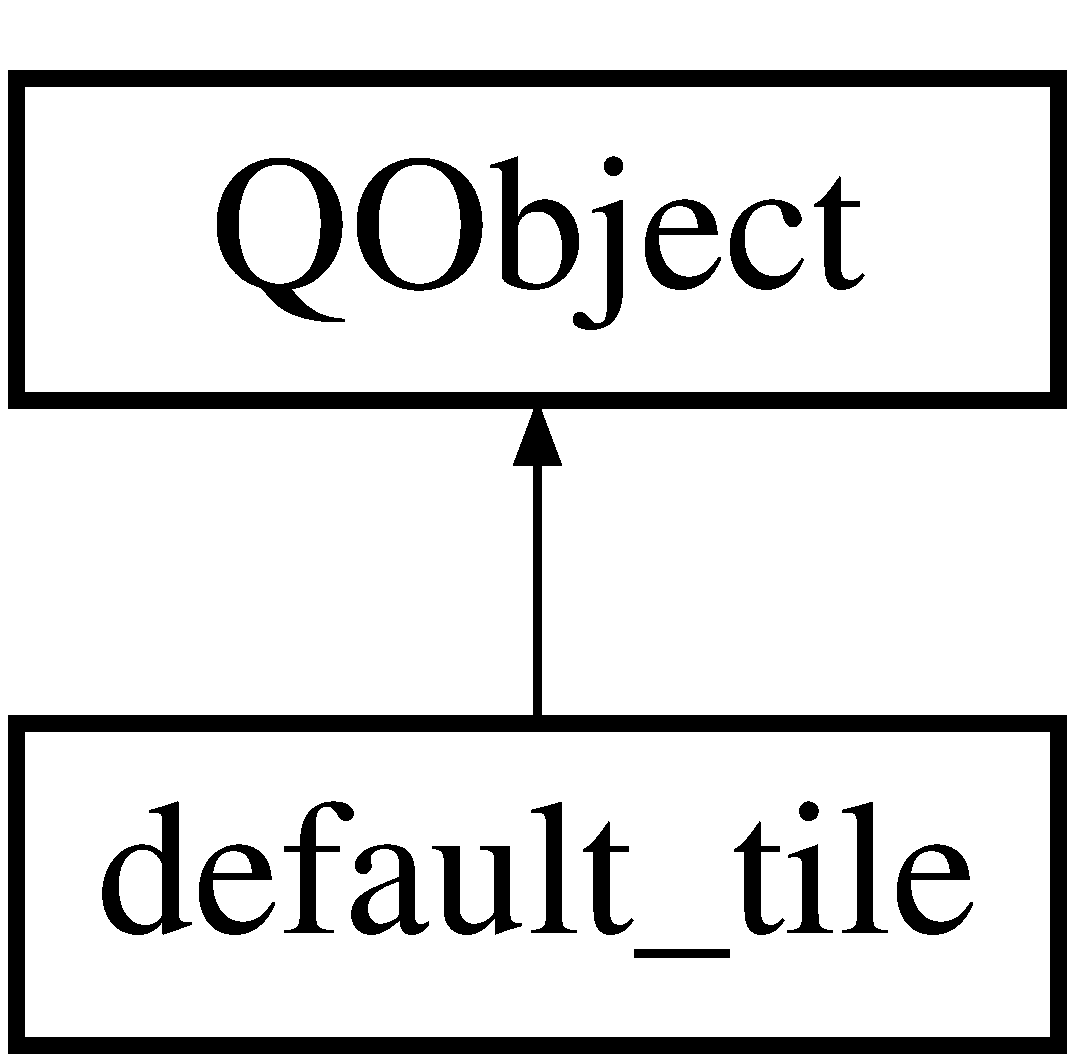
\includegraphics[height=2.000000cm]{classdefault__tile}
\end{center}
\end{figure}
\subsection*{Public Member Functions}
\begin{DoxyCompactItemize}
\item 
\hyperlink{classdefault__tile_a95ff4527fa0b82da41b8ac27aa19b303}{default\-\_\-tile} ()
\begin{DoxyCompactList}\small\item\em Test setup. \end{DoxyCompactList}\end{DoxyCompactItemize}
\subsection*{Private Slots}
\begin{DoxyCompactItemize}
\item 
void \hyperlink{classdefault__tile_a43bdf803d694109b43b391aa0420d046}{test\-\_\-add\-Building} ()
\begin{DoxyCompactList}\small\item\em Tests adding a building to a tile. \end{DoxyCompactList}\item 
void \hyperlink{classdefault__tile_a77367549be5fa7a7e0d30da6ef87cb4e}{test\-\_\-add\-Building\-\_\-too\-\_\-many\-\_\-buildings} ()
\begin{DoxyCompactList}\small\item\em Tests adding too many buildings on a tile. \end{DoxyCompactList}\item 
void \hyperlink{classdefault__tile_ac5b6391d1b5eb66bcb20bf17dcbb1c79}{test\-\_\-add\-Building\-\_\-to\-\_\-water} ()
\begin{DoxyCompactList}\small\item\em Tests adding a building to water. \end{DoxyCompactList}\item 
void \hyperlink{classdefault__tile_a692ffdcc135066c0099af99c72073768}{test\-\_\-remove\-Building} ()
\begin{DoxyCompactList}\small\item\em Tests removing a building from a tile. \end{DoxyCompactList}\item 
void \hyperlink{classdefault__tile_a3af682c7eb40ea93a2c99abc55a9b45e}{test\-\_\-get\-Buildings} ()
\begin{DoxyCompactList}\small\item\em Tests getting buildings from a tile. \end{DoxyCompactList}\item 
void \hyperlink{classdefault__tile_ac2868337bc13dea171895916e375a0d8}{test\-\_\-add\-Worker} ()
\begin{DoxyCompactList}\small\item\em Tests adding a worker to a tile. \end{DoxyCompactList}\item 
void \hyperlink{classdefault__tile_af65fe1d9ce7dfe3706b434cf7650eb06}{test\-\_\-add\-Worker\-\_\-too\-\_\-many\-\_\-workers} ()
\begin{DoxyCompactList}\small\item\em Tests adding too many workers on a tile. \end{DoxyCompactList}\item 
void \hyperlink{classdefault__tile_a29665a14d12c952675435a9bd642bc06}{test\-\_\-add\-Worker\-\_\-to\-\_\-water} ()
\begin{DoxyCompactList}\small\item\em Tests adding a worker to water. \end{DoxyCompactList}\item 
void \hyperlink{classdefault__tile_aee9fffb30a5ca5435a5421c548b1f9e5}{test\-\_\-remove\-Worker} ()
\begin{DoxyCompactList}\small\item\em Tests removing a worker from a tile. \end{DoxyCompactList}\item 
void \hyperlink{classdefault__tile_a57d1f35c44e5c82d4ca2878795fb0890}{test\-\_\-get\-Workers} ()
\begin{DoxyCompactList}\small\item\em Tests getting workers from a tile. \end{DoxyCompactList}\item 
void \hyperlink{classdefault__tile_a917f002ab0713044a752be2f6a37d6ff}{test\-\_\-add\-Building\-And\-Worker} ()
\begin{DoxyCompactList}\small\item\em Tests adding workers and buildings to a tile. \end{DoxyCompactList}\item 
void \hyperlink{classdefault__tile_a2fa5ec48fde3f3ba7952d364c179ad65}{test\-\_\-type\-\_\-tilebase} ()
\begin{DoxyCompactList}\small\item\em Tests Tiles\-Base's type. \end{DoxyCompactList}\item 
void \hyperlink{classdefault__tile_abc9cdbb32628185b44a1610454054da7}{test\-\_\-type\-\_\-forest} ()
\begin{DoxyCompactList}\small\item\em Tests Forest's type. \end{DoxyCompactList}\item 
void \hyperlink{classdefault__tile_a5383699e1c9a86e7414cd477b922fbd5}{test\-\_\-type\-\_\-grassland} ()
\begin{DoxyCompactList}\small\item\em Tests Grassland's type. \end{DoxyCompactList}\item 
void \hyperlink{classdefault__tile_a086986610e729ee878f8c68b4b19d10b}{test\-\_\-type\-\_\-water} ()
\begin{DoxyCompactList}\small\item\em Tests Water's type. \end{DoxyCompactList}\item 
void \hyperlink{classdefault__tile_a6612daefb98dbb72a1860264b87f0dbb}{test\-\_\-type\-\_\-blockfield} ()
\begin{DoxyCompactList}\small\item\em Tests Blockfield's type. \end{DoxyCompactList}\item 
void \hyperlink{classdefault__tile_a05d5665f788e8d38f6708725c9ee946b}{test\-\_\-type\-\_\-oredeposit} ()
\begin{DoxyCompactList}\small\item\em Tests Ore\-Deposit's type. \end{DoxyCompactList}\item 
void \hyperlink{classdefault__tile_ab2c7a242550d5a341cfbef3cb9d83990}{cleanup} ()
\begin{DoxyCompactList}\small\item\em Test cleanup. \end{DoxyCompactList}\end{DoxyCompactItemize}
\subsection*{Private Attributes}
\begin{DoxyCompactItemize}
\item 
std\-::shared\-\_\-ptr$<$ \hyperlink{classGame_1_1ObjectManager}{Object\-Manager} $>$ \hyperlink{classdefault__tile_a8749ee4ac9c528916c2fd835ce14f043}{obj\-Man}
\item 
std\-::shared\-\_\-ptr$<$ \hyperlink{classGame_1_1GameEventHandler}{Game\-Event\-Handler} $>$ \hyperlink{classdefault__tile_ac2682ad79db9879a601bc5bdd24add2c}{G\-E\-Hand}
\item 
std\-::shared\-\_\-ptr$<$ \hyperlink{classGame_1_1Player}{Player} $>$ \hyperlink{classdefault__tile_adeba3a9d85b478d7cd0dbd5b6194ede3}{player1}
\item 
std\-::shared\-\_\-ptr$<$ \hyperlink{classGame_1_1Player}{Player} $>$ \hyperlink{classdefault__tile_ad7407fc63175dce0d369ddcc261194a6}{player2}
\item 
std\-::shared\-\_\-ptr\\*
$<$ \hyperlink{classCourse_1_1BuildingBase}{Course\-::\-Building\-Base} $>$ \hyperlink{classdefault__tile_a1428f399558ca156afbc754ae04fe6d0}{building1}
\item 
std\-::shared\-\_\-ptr\\*
$<$ \hyperlink{classCourse_1_1BuildingBase}{Course\-::\-Building\-Base} $>$ \hyperlink{classdefault__tile_a6cff7bada2d7f8f055225d1442fc0d6d}{building2}
\item 
std\-::shared\-\_\-ptr\\*
$<$ \hyperlink{classCourse_1_1BasicWorker}{Course\-::\-Basic\-Worker} $>$ \hyperlink{classdefault__tile_a15da0582e401dfe74e37fc3d6e27931a}{worker1}
\item 
std\-::shared\-\_\-ptr\\*
$<$ \hyperlink{classCourse_1_1BasicWorker}{Course\-::\-Basic\-Worker} $>$ \hyperlink{classdefault__tile_ace6e1dbaff450508a5889ccc10190da5}{worker2}
\item 
std\-::shared\-\_\-ptr$<$ \hyperlink{classCourse_1_1TileBase}{Course\-::\-Tile\-Base} $>$ \hyperlink{classdefault__tile_af0e444a7cbe271a0eca9a245fcd938ff}{default\-\_\-object}
\item 
std\-::shared\-\_\-ptr$<$ \hyperlink{classCourse_1_1Forest}{Course\-::\-Forest} $>$ \hyperlink{classdefault__tile_aed6aefdcd6b8d7ebf30d586e9143d44f}{forest\-\_\-object}
\item 
std\-::shared\-\_\-ptr\\*
$<$ \hyperlink{classCourse_1_1Grassland}{Course\-::\-Grassland} $>$ \hyperlink{classdefault__tile_ad5fbacd1a3d966e10aa6127db0ba3213}{grassland\-\_\-object}
\item 
std\-::shared\-\_\-ptr$<$ \hyperlink{classGame_1_1Blockfield}{Blockfield} $>$ \hyperlink{classdefault__tile_a475f12ebc676bc8252ccea358329eb55}{blockfield\-\_\-object}
\item 
std\-::shared\-\_\-ptr$<$ \hyperlink{classGame_1_1OreDeposit}{Ore\-Deposit} $>$ \hyperlink{classdefault__tile_a267580dfeea7352f56f5bd106def49c5}{oredeposit\-\_\-object}
\item 
std\-::shared\-\_\-ptr$<$ \hyperlink{classGame_1_1Water}{Water} $>$ \hyperlink{classdefault__tile_a083dbfdbbd2f789667ce742cb26afe83}{water\-\_\-object}
\item 
const \hyperlink{classCourse_1_1Coordinate}{Course\-::\-Coordinate} \hyperlink{classdefault__tile_ad881db4d38fb6ce5f6344fd13ad35fc1}{coord1} = \{1,1\}
\item 
const \hyperlink{classCourse_1_1Coordinate}{Course\-::\-Coordinate} \hyperlink{classdefault__tile_afe8df9f0be2707e28ca52f2d63a6f565}{coord2} = \{2,2\}
\item 
const \hyperlink{classCourse_1_1Coordinate}{Course\-::\-Coordinate} \hyperlink{classdefault__tile_ad831dcb7909d9e7918380ed7ec7f0f8b}{coord3} = \{3,3\}
\item 
const \hyperlink{classCourse_1_1Coordinate}{Course\-::\-Coordinate} \hyperlink{classdefault__tile_adfe1e7d47661ef24230ed213d6860d0d}{coord4} = \{4,4\}
\item 
const \hyperlink{classCourse_1_1Coordinate}{Course\-::\-Coordinate} \hyperlink{classdefault__tile_a99eb8e09cd1e8bc821c1d410f0cefcdc}{coord5} = \{5,5\}
\item 
const \hyperlink{classCourse_1_1Coordinate}{Course\-::\-Coordinate} \hyperlink{classdefault__tile_a02b5556e362bb56edb63015f8a57aaa1}{coord6} = \{6,6\}
\end{DoxyCompactItemize}


\subsection{Detailed Description}
The tiles\-\_\-tests test the Tile\-Base class and all its children. 

\subsection{Constructor \& Destructor Documentation}
\hypertarget{classdefault__tile_a95ff4527fa0b82da41b8ac27aa19b303}{\index{default\-\_\-tile@{default\-\_\-tile}!default\-\_\-tile@{default\-\_\-tile}}
\index{default\-\_\-tile@{default\-\_\-tile}!default_tile@{default\-\_\-tile}}
\subsubsection[{default\-\_\-tile}]{\setlength{\rightskip}{0pt plus 5cm}default\-\_\-tile\-::default\-\_\-tile (
\begin{DoxyParamCaption}
{}
\end{DoxyParamCaption}
)}}\label{classdefault__tile_a95ff4527fa0b82da41b8ac27aa19b303}


Test setup. 



\subsection{Member Function Documentation}
\hypertarget{classdefault__tile_ab2c7a242550d5a341cfbef3cb9d83990}{\index{default\-\_\-tile@{default\-\_\-tile}!cleanup@{cleanup}}
\index{cleanup@{cleanup}!default_tile@{default\-\_\-tile}}
\subsubsection[{cleanup}]{\setlength{\rightskip}{0pt plus 5cm}void default\-\_\-tile\-::cleanup (
\begin{DoxyParamCaption}
{}
\end{DoxyParamCaption}
)\hspace{0.3cm}{\ttfamily [private]}, {\ttfamily [slot]}}}\label{classdefault__tile_ab2c7a242550d5a341cfbef3cb9d83990}


Test cleanup. 

\hypertarget{classdefault__tile_a43bdf803d694109b43b391aa0420d046}{\index{default\-\_\-tile@{default\-\_\-tile}!test\-\_\-add\-Building@{test\-\_\-add\-Building}}
\index{test\-\_\-add\-Building@{test\-\_\-add\-Building}!default_tile@{default\-\_\-tile}}
\subsubsection[{test\-\_\-add\-Building}]{\setlength{\rightskip}{0pt plus 5cm}void default\-\_\-tile\-::test\-\_\-add\-Building (
\begin{DoxyParamCaption}
{}
\end{DoxyParamCaption}
)\hspace{0.3cm}{\ttfamily [private]}, {\ttfamily [slot]}}}\label{classdefault__tile_a43bdf803d694109b43b391aa0420d046}


Tests adding a building to a tile. 

\begin{DoxyPostcond}{Postcondition}
Should be possible 
\end{DoxyPostcond}
\hypertarget{classdefault__tile_ac5b6391d1b5eb66bcb20bf17dcbb1c79}{\index{default\-\_\-tile@{default\-\_\-tile}!test\-\_\-add\-Building\-\_\-to\-\_\-water@{test\-\_\-add\-Building\-\_\-to\-\_\-water}}
\index{test\-\_\-add\-Building\-\_\-to\-\_\-water@{test\-\_\-add\-Building\-\_\-to\-\_\-water}!default_tile@{default\-\_\-tile}}
\subsubsection[{test\-\_\-add\-Building\-\_\-to\-\_\-water}]{\setlength{\rightskip}{0pt plus 5cm}void default\-\_\-tile\-::test\-\_\-add\-Building\-\_\-to\-\_\-water (
\begin{DoxyParamCaption}
{}
\end{DoxyParamCaption}
)\hspace{0.3cm}{\ttfamily [private]}, {\ttfamily [slot]}}}\label{classdefault__tile_ac5b6391d1b5eb66bcb20bf17dcbb1c79}


Tests adding a building to water. 

\begin{DoxyPostcond}{Postcondition}
Should throw an Illegal\-Action exception 
\end{DoxyPostcond}
\hypertarget{classdefault__tile_a77367549be5fa7a7e0d30da6ef87cb4e}{\index{default\-\_\-tile@{default\-\_\-tile}!test\-\_\-add\-Building\-\_\-too\-\_\-many\-\_\-buildings@{test\-\_\-add\-Building\-\_\-too\-\_\-many\-\_\-buildings}}
\index{test\-\_\-add\-Building\-\_\-too\-\_\-many\-\_\-buildings@{test\-\_\-add\-Building\-\_\-too\-\_\-many\-\_\-buildings}!default_tile@{default\-\_\-tile}}
\subsubsection[{test\-\_\-add\-Building\-\_\-too\-\_\-many\-\_\-buildings}]{\setlength{\rightskip}{0pt plus 5cm}void default\-\_\-tile\-::test\-\_\-add\-Building\-\_\-too\-\_\-many\-\_\-buildings (
\begin{DoxyParamCaption}
{}
\end{DoxyParamCaption}
)\hspace{0.3cm}{\ttfamily [private]}, {\ttfamily [slot]}}}\label{classdefault__tile_a77367549be5fa7a7e0d30da6ef87cb4e}


Tests adding too many buildings on a tile. 

\begin{DoxyPostcond}{Postcondition}
Should throw an Illegal\-Action exception 
\end{DoxyPostcond}
\hypertarget{classdefault__tile_a917f002ab0713044a752be2f6a37d6ff}{\index{default\-\_\-tile@{default\-\_\-tile}!test\-\_\-add\-Building\-And\-Worker@{test\-\_\-add\-Building\-And\-Worker}}
\index{test\-\_\-add\-Building\-And\-Worker@{test\-\_\-add\-Building\-And\-Worker}!default_tile@{default\-\_\-tile}}
\subsubsection[{test\-\_\-add\-Building\-And\-Worker}]{\setlength{\rightskip}{0pt plus 5cm}void default\-\_\-tile\-::test\-\_\-add\-Building\-And\-Worker (
\begin{DoxyParamCaption}
{}
\end{DoxyParamCaption}
)\hspace{0.3cm}{\ttfamily [private]}, {\ttfamily [slot]}}}\label{classdefault__tile_a917f002ab0713044a752be2f6a37d6ff}


Tests adding workers and buildings to a tile. 

\begin{DoxyPostcond}{Postcondition}
Should be possible to add both within limits of the tile 
\end{DoxyPostcond}
\hypertarget{classdefault__tile_ac2868337bc13dea171895916e375a0d8}{\index{default\-\_\-tile@{default\-\_\-tile}!test\-\_\-add\-Worker@{test\-\_\-add\-Worker}}
\index{test\-\_\-add\-Worker@{test\-\_\-add\-Worker}!default_tile@{default\-\_\-tile}}
\subsubsection[{test\-\_\-add\-Worker}]{\setlength{\rightskip}{0pt plus 5cm}void default\-\_\-tile\-::test\-\_\-add\-Worker (
\begin{DoxyParamCaption}
{}
\end{DoxyParamCaption}
)\hspace{0.3cm}{\ttfamily [private]}, {\ttfamily [slot]}}}\label{classdefault__tile_ac2868337bc13dea171895916e375a0d8}


Tests adding a worker to a tile. 

\begin{DoxyPostcond}{Postcondition}
Should be possible 
\end{DoxyPostcond}
\hypertarget{classdefault__tile_a29665a14d12c952675435a9bd642bc06}{\index{default\-\_\-tile@{default\-\_\-tile}!test\-\_\-add\-Worker\-\_\-to\-\_\-water@{test\-\_\-add\-Worker\-\_\-to\-\_\-water}}
\index{test\-\_\-add\-Worker\-\_\-to\-\_\-water@{test\-\_\-add\-Worker\-\_\-to\-\_\-water}!default_tile@{default\-\_\-tile}}
\subsubsection[{test\-\_\-add\-Worker\-\_\-to\-\_\-water}]{\setlength{\rightskip}{0pt plus 5cm}void default\-\_\-tile\-::test\-\_\-add\-Worker\-\_\-to\-\_\-water (
\begin{DoxyParamCaption}
{}
\end{DoxyParamCaption}
)\hspace{0.3cm}{\ttfamily [private]}, {\ttfamily [slot]}}}\label{classdefault__tile_a29665a14d12c952675435a9bd642bc06}


Tests adding a worker to water. 

\begin{DoxyPostcond}{Postcondition}
Should throw an Illegal\-Action exception 
\end{DoxyPostcond}
\hypertarget{classdefault__tile_af65fe1d9ce7dfe3706b434cf7650eb06}{\index{default\-\_\-tile@{default\-\_\-tile}!test\-\_\-add\-Worker\-\_\-too\-\_\-many\-\_\-workers@{test\-\_\-add\-Worker\-\_\-too\-\_\-many\-\_\-workers}}
\index{test\-\_\-add\-Worker\-\_\-too\-\_\-many\-\_\-workers@{test\-\_\-add\-Worker\-\_\-too\-\_\-many\-\_\-workers}!default_tile@{default\-\_\-tile}}
\subsubsection[{test\-\_\-add\-Worker\-\_\-too\-\_\-many\-\_\-workers}]{\setlength{\rightskip}{0pt plus 5cm}void default\-\_\-tile\-::test\-\_\-add\-Worker\-\_\-too\-\_\-many\-\_\-workers (
\begin{DoxyParamCaption}
{}
\end{DoxyParamCaption}
)\hspace{0.3cm}{\ttfamily [private]}, {\ttfamily [slot]}}}\label{classdefault__tile_af65fe1d9ce7dfe3706b434cf7650eb06}


Tests adding too many workers on a tile. 

\begin{DoxyPostcond}{Postcondition}
Should throw an Illegal\-Action exception 
\end{DoxyPostcond}
\hypertarget{classdefault__tile_a3af682c7eb40ea93a2c99abc55a9b45e}{\index{default\-\_\-tile@{default\-\_\-tile}!test\-\_\-get\-Buildings@{test\-\_\-get\-Buildings}}
\index{test\-\_\-get\-Buildings@{test\-\_\-get\-Buildings}!default_tile@{default\-\_\-tile}}
\subsubsection[{test\-\_\-get\-Buildings}]{\setlength{\rightskip}{0pt plus 5cm}void default\-\_\-tile\-::test\-\_\-get\-Buildings (
\begin{DoxyParamCaption}
{}
\end{DoxyParamCaption}
)\hspace{0.3cm}{\ttfamily [private]}, {\ttfamily [slot]}}}\label{classdefault__tile_a3af682c7eb40ea93a2c99abc55a9b45e}


Tests getting buildings from a tile. 

\begin{DoxyPostcond}{Postcondition}
Should be possible 
\end{DoxyPostcond}
\hypertarget{classdefault__tile_a57d1f35c44e5c82d4ca2878795fb0890}{\index{default\-\_\-tile@{default\-\_\-tile}!test\-\_\-get\-Workers@{test\-\_\-get\-Workers}}
\index{test\-\_\-get\-Workers@{test\-\_\-get\-Workers}!default_tile@{default\-\_\-tile}}
\subsubsection[{test\-\_\-get\-Workers}]{\setlength{\rightskip}{0pt plus 5cm}void default\-\_\-tile\-::test\-\_\-get\-Workers (
\begin{DoxyParamCaption}
{}
\end{DoxyParamCaption}
)\hspace{0.3cm}{\ttfamily [private]}, {\ttfamily [slot]}}}\label{classdefault__tile_a57d1f35c44e5c82d4ca2878795fb0890}


Tests getting workers from a tile. 

\begin{DoxyPostcond}{Postcondition}
Should be possible 
\end{DoxyPostcond}
\hypertarget{classdefault__tile_a692ffdcc135066c0099af99c72073768}{\index{default\-\_\-tile@{default\-\_\-tile}!test\-\_\-remove\-Building@{test\-\_\-remove\-Building}}
\index{test\-\_\-remove\-Building@{test\-\_\-remove\-Building}!default_tile@{default\-\_\-tile}}
\subsubsection[{test\-\_\-remove\-Building}]{\setlength{\rightskip}{0pt plus 5cm}void default\-\_\-tile\-::test\-\_\-remove\-Building (
\begin{DoxyParamCaption}
{}
\end{DoxyParamCaption}
)\hspace{0.3cm}{\ttfamily [private]}, {\ttfamily [slot]}}}\label{classdefault__tile_a692ffdcc135066c0099af99c72073768}


Tests removing a building from a tile. 

\begin{DoxyPostcond}{Postcondition}
Should be possible 
\end{DoxyPostcond}
\hypertarget{classdefault__tile_aee9fffb30a5ca5435a5421c548b1f9e5}{\index{default\-\_\-tile@{default\-\_\-tile}!test\-\_\-remove\-Worker@{test\-\_\-remove\-Worker}}
\index{test\-\_\-remove\-Worker@{test\-\_\-remove\-Worker}!default_tile@{default\-\_\-tile}}
\subsubsection[{test\-\_\-remove\-Worker}]{\setlength{\rightskip}{0pt plus 5cm}void default\-\_\-tile\-::test\-\_\-remove\-Worker (
\begin{DoxyParamCaption}
{}
\end{DoxyParamCaption}
)\hspace{0.3cm}{\ttfamily [private]}, {\ttfamily [slot]}}}\label{classdefault__tile_aee9fffb30a5ca5435a5421c548b1f9e5}


Tests removing a worker from a tile. 

\begin{DoxyPostcond}{Postcondition}
Should be possible 
\end{DoxyPostcond}
\hypertarget{classdefault__tile_a6612daefb98dbb72a1860264b87f0dbb}{\index{default\-\_\-tile@{default\-\_\-tile}!test\-\_\-type\-\_\-blockfield@{test\-\_\-type\-\_\-blockfield}}
\index{test\-\_\-type\-\_\-blockfield@{test\-\_\-type\-\_\-blockfield}!default_tile@{default\-\_\-tile}}
\subsubsection[{test\-\_\-type\-\_\-blockfield}]{\setlength{\rightskip}{0pt plus 5cm}void default\-\_\-tile\-::test\-\_\-type\-\_\-blockfield (
\begin{DoxyParamCaption}
{}
\end{DoxyParamCaption}
)\hspace{0.3cm}{\ttfamily [private]}, {\ttfamily [slot]}}}\label{classdefault__tile_a6612daefb98dbb72a1860264b87f0dbb}


Tests Blockfield's type. 

\begin{DoxyPostcond}{Postcondition}
Should be Blockfield 
\end{DoxyPostcond}
\hypertarget{classdefault__tile_abc9cdbb32628185b44a1610454054da7}{\index{default\-\_\-tile@{default\-\_\-tile}!test\-\_\-type\-\_\-forest@{test\-\_\-type\-\_\-forest}}
\index{test\-\_\-type\-\_\-forest@{test\-\_\-type\-\_\-forest}!default_tile@{default\-\_\-tile}}
\subsubsection[{test\-\_\-type\-\_\-forest}]{\setlength{\rightskip}{0pt plus 5cm}void default\-\_\-tile\-::test\-\_\-type\-\_\-forest (
\begin{DoxyParamCaption}
{}
\end{DoxyParamCaption}
)\hspace{0.3cm}{\ttfamily [private]}, {\ttfamily [slot]}}}\label{classdefault__tile_abc9cdbb32628185b44a1610454054da7}


Tests Forest's type. 

\begin{DoxyPostcond}{Postcondition}
Should be Forest 
\end{DoxyPostcond}
\hypertarget{classdefault__tile_a5383699e1c9a86e7414cd477b922fbd5}{\index{default\-\_\-tile@{default\-\_\-tile}!test\-\_\-type\-\_\-grassland@{test\-\_\-type\-\_\-grassland}}
\index{test\-\_\-type\-\_\-grassland@{test\-\_\-type\-\_\-grassland}!default_tile@{default\-\_\-tile}}
\subsubsection[{test\-\_\-type\-\_\-grassland}]{\setlength{\rightskip}{0pt plus 5cm}void default\-\_\-tile\-::test\-\_\-type\-\_\-grassland (
\begin{DoxyParamCaption}
{}
\end{DoxyParamCaption}
)\hspace{0.3cm}{\ttfamily [private]}, {\ttfamily [slot]}}}\label{classdefault__tile_a5383699e1c9a86e7414cd477b922fbd5}


Tests Grassland's type. 

\begin{DoxyPostcond}{Postcondition}
Should be Grassland 
\end{DoxyPostcond}
\hypertarget{classdefault__tile_a05d5665f788e8d38f6708725c9ee946b}{\index{default\-\_\-tile@{default\-\_\-tile}!test\-\_\-type\-\_\-oredeposit@{test\-\_\-type\-\_\-oredeposit}}
\index{test\-\_\-type\-\_\-oredeposit@{test\-\_\-type\-\_\-oredeposit}!default_tile@{default\-\_\-tile}}
\subsubsection[{test\-\_\-type\-\_\-oredeposit}]{\setlength{\rightskip}{0pt plus 5cm}void default\-\_\-tile\-::test\-\_\-type\-\_\-oredeposit (
\begin{DoxyParamCaption}
{}
\end{DoxyParamCaption}
)\hspace{0.3cm}{\ttfamily [private]}, {\ttfamily [slot]}}}\label{classdefault__tile_a05d5665f788e8d38f6708725c9ee946b}


Tests Ore\-Deposit's type. 

\begin{DoxyPostcond}{Postcondition}
Should be Ore\-Deposit 
\end{DoxyPostcond}
\hypertarget{classdefault__tile_a2fa5ec48fde3f3ba7952d364c179ad65}{\index{default\-\_\-tile@{default\-\_\-tile}!test\-\_\-type\-\_\-tilebase@{test\-\_\-type\-\_\-tilebase}}
\index{test\-\_\-type\-\_\-tilebase@{test\-\_\-type\-\_\-tilebase}!default_tile@{default\-\_\-tile}}
\subsubsection[{test\-\_\-type\-\_\-tilebase}]{\setlength{\rightskip}{0pt plus 5cm}void default\-\_\-tile\-::test\-\_\-type\-\_\-tilebase (
\begin{DoxyParamCaption}
{}
\end{DoxyParamCaption}
)\hspace{0.3cm}{\ttfamily [private]}, {\ttfamily [slot]}}}\label{classdefault__tile_a2fa5ec48fde3f3ba7952d364c179ad65}


Tests Tiles\-Base's type. 

\begin{DoxyPostcond}{Postcondition}
Should be Tiles\-Base 
\end{DoxyPostcond}
\hypertarget{classdefault__tile_a086986610e729ee878f8c68b4b19d10b}{\index{default\-\_\-tile@{default\-\_\-tile}!test\-\_\-type\-\_\-water@{test\-\_\-type\-\_\-water}}
\index{test\-\_\-type\-\_\-water@{test\-\_\-type\-\_\-water}!default_tile@{default\-\_\-tile}}
\subsubsection[{test\-\_\-type\-\_\-water}]{\setlength{\rightskip}{0pt plus 5cm}void default\-\_\-tile\-::test\-\_\-type\-\_\-water (
\begin{DoxyParamCaption}
{}
\end{DoxyParamCaption}
)\hspace{0.3cm}{\ttfamily [private]}, {\ttfamily [slot]}}}\label{classdefault__tile_a086986610e729ee878f8c68b4b19d10b}


Tests Water's type. 

\begin{DoxyPostcond}{Postcondition}
Should be Water 
\end{DoxyPostcond}


\subsection{Member Data Documentation}
\hypertarget{classdefault__tile_a475f12ebc676bc8252ccea358329eb55}{\index{default\-\_\-tile@{default\-\_\-tile}!blockfield\-\_\-object@{blockfield\-\_\-object}}
\index{blockfield\-\_\-object@{blockfield\-\_\-object}!default_tile@{default\-\_\-tile}}
\subsubsection[{blockfield\-\_\-object}]{\setlength{\rightskip}{0pt plus 5cm}std\-::shared\-\_\-ptr$<${\bf Blockfield}$>$ default\-\_\-tile\-::blockfield\-\_\-object\hspace{0.3cm}{\ttfamily [private]}}}\label{classdefault__tile_a475f12ebc676bc8252ccea358329eb55}
\hypertarget{classdefault__tile_a1428f399558ca156afbc754ae04fe6d0}{\index{default\-\_\-tile@{default\-\_\-tile}!building1@{building1}}
\index{building1@{building1}!default_tile@{default\-\_\-tile}}
\subsubsection[{building1}]{\setlength{\rightskip}{0pt plus 5cm}std\-::shared\-\_\-ptr$<${\bf Course\-::\-Building\-Base}$>$ default\-\_\-tile\-::building1\hspace{0.3cm}{\ttfamily [private]}}}\label{classdefault__tile_a1428f399558ca156afbc754ae04fe6d0}
\hypertarget{classdefault__tile_a6cff7bada2d7f8f055225d1442fc0d6d}{\index{default\-\_\-tile@{default\-\_\-tile}!building2@{building2}}
\index{building2@{building2}!default_tile@{default\-\_\-tile}}
\subsubsection[{building2}]{\setlength{\rightskip}{0pt plus 5cm}std\-::shared\-\_\-ptr$<${\bf Course\-::\-Building\-Base}$>$ default\-\_\-tile\-::building2\hspace{0.3cm}{\ttfamily [private]}}}\label{classdefault__tile_a6cff7bada2d7f8f055225d1442fc0d6d}
\hypertarget{classdefault__tile_ad881db4d38fb6ce5f6344fd13ad35fc1}{\index{default\-\_\-tile@{default\-\_\-tile}!coord1@{coord1}}
\index{coord1@{coord1}!default_tile@{default\-\_\-tile}}
\subsubsection[{coord1}]{\setlength{\rightskip}{0pt plus 5cm}const {\bf Course\-::\-Coordinate} default\-\_\-tile\-::coord1 = \{1,1\}\hspace{0.3cm}{\ttfamily [private]}}}\label{classdefault__tile_ad881db4d38fb6ce5f6344fd13ad35fc1}
\hypertarget{classdefault__tile_afe8df9f0be2707e28ca52f2d63a6f565}{\index{default\-\_\-tile@{default\-\_\-tile}!coord2@{coord2}}
\index{coord2@{coord2}!default_tile@{default\-\_\-tile}}
\subsubsection[{coord2}]{\setlength{\rightskip}{0pt plus 5cm}const {\bf Course\-::\-Coordinate} default\-\_\-tile\-::coord2 = \{2,2\}\hspace{0.3cm}{\ttfamily [private]}}}\label{classdefault__tile_afe8df9f0be2707e28ca52f2d63a6f565}
\hypertarget{classdefault__tile_ad831dcb7909d9e7918380ed7ec7f0f8b}{\index{default\-\_\-tile@{default\-\_\-tile}!coord3@{coord3}}
\index{coord3@{coord3}!default_tile@{default\-\_\-tile}}
\subsubsection[{coord3}]{\setlength{\rightskip}{0pt plus 5cm}const {\bf Course\-::\-Coordinate} default\-\_\-tile\-::coord3 = \{3,3\}\hspace{0.3cm}{\ttfamily [private]}}}\label{classdefault__tile_ad831dcb7909d9e7918380ed7ec7f0f8b}
\hypertarget{classdefault__tile_adfe1e7d47661ef24230ed213d6860d0d}{\index{default\-\_\-tile@{default\-\_\-tile}!coord4@{coord4}}
\index{coord4@{coord4}!default_tile@{default\-\_\-tile}}
\subsubsection[{coord4}]{\setlength{\rightskip}{0pt plus 5cm}const {\bf Course\-::\-Coordinate} default\-\_\-tile\-::coord4 = \{4,4\}\hspace{0.3cm}{\ttfamily [private]}}}\label{classdefault__tile_adfe1e7d47661ef24230ed213d6860d0d}
\hypertarget{classdefault__tile_a99eb8e09cd1e8bc821c1d410f0cefcdc}{\index{default\-\_\-tile@{default\-\_\-tile}!coord5@{coord5}}
\index{coord5@{coord5}!default_tile@{default\-\_\-tile}}
\subsubsection[{coord5}]{\setlength{\rightskip}{0pt plus 5cm}const {\bf Course\-::\-Coordinate} default\-\_\-tile\-::coord5 = \{5,5\}\hspace{0.3cm}{\ttfamily [private]}}}\label{classdefault__tile_a99eb8e09cd1e8bc821c1d410f0cefcdc}
\hypertarget{classdefault__tile_a02b5556e362bb56edb63015f8a57aaa1}{\index{default\-\_\-tile@{default\-\_\-tile}!coord6@{coord6}}
\index{coord6@{coord6}!default_tile@{default\-\_\-tile}}
\subsubsection[{coord6}]{\setlength{\rightskip}{0pt plus 5cm}const {\bf Course\-::\-Coordinate} default\-\_\-tile\-::coord6 = \{6,6\}\hspace{0.3cm}{\ttfamily [private]}}}\label{classdefault__tile_a02b5556e362bb56edb63015f8a57aaa1}
\hypertarget{classdefault__tile_af0e444a7cbe271a0eca9a245fcd938ff}{\index{default\-\_\-tile@{default\-\_\-tile}!default\-\_\-object@{default\-\_\-object}}
\index{default\-\_\-object@{default\-\_\-object}!default_tile@{default\-\_\-tile}}
\subsubsection[{default\-\_\-object}]{\setlength{\rightskip}{0pt plus 5cm}std\-::shared\-\_\-ptr$<${\bf Course\-::\-Tile\-Base}$>$ default\-\_\-tile\-::default\-\_\-object\hspace{0.3cm}{\ttfamily [private]}}}\label{classdefault__tile_af0e444a7cbe271a0eca9a245fcd938ff}
\hypertarget{classdefault__tile_aed6aefdcd6b8d7ebf30d586e9143d44f}{\index{default\-\_\-tile@{default\-\_\-tile}!forest\-\_\-object@{forest\-\_\-object}}
\index{forest\-\_\-object@{forest\-\_\-object}!default_tile@{default\-\_\-tile}}
\subsubsection[{forest\-\_\-object}]{\setlength{\rightskip}{0pt plus 5cm}std\-::shared\-\_\-ptr$<${\bf Course\-::\-Forest}$>$ default\-\_\-tile\-::forest\-\_\-object\hspace{0.3cm}{\ttfamily [private]}}}\label{classdefault__tile_aed6aefdcd6b8d7ebf30d586e9143d44f}
\hypertarget{classdefault__tile_ac2682ad79db9879a601bc5bdd24add2c}{\index{default\-\_\-tile@{default\-\_\-tile}!G\-E\-Hand@{G\-E\-Hand}}
\index{G\-E\-Hand@{G\-E\-Hand}!default_tile@{default\-\_\-tile}}
\subsubsection[{G\-E\-Hand}]{\setlength{\rightskip}{0pt plus 5cm}std\-::shared\-\_\-ptr$<${\bf Game\-Event\-Handler}$>$ default\-\_\-tile\-::\-G\-E\-Hand\hspace{0.3cm}{\ttfamily [private]}}}\label{classdefault__tile_ac2682ad79db9879a601bc5bdd24add2c}
\hypertarget{classdefault__tile_ad5fbacd1a3d966e10aa6127db0ba3213}{\index{default\-\_\-tile@{default\-\_\-tile}!grassland\-\_\-object@{grassland\-\_\-object}}
\index{grassland\-\_\-object@{grassland\-\_\-object}!default_tile@{default\-\_\-tile}}
\subsubsection[{grassland\-\_\-object}]{\setlength{\rightskip}{0pt plus 5cm}std\-::shared\-\_\-ptr$<${\bf Course\-::\-Grassland}$>$ default\-\_\-tile\-::grassland\-\_\-object\hspace{0.3cm}{\ttfamily [private]}}}\label{classdefault__tile_ad5fbacd1a3d966e10aa6127db0ba3213}
\hypertarget{classdefault__tile_a8749ee4ac9c528916c2fd835ce14f043}{\index{default\-\_\-tile@{default\-\_\-tile}!obj\-Man@{obj\-Man}}
\index{obj\-Man@{obj\-Man}!default_tile@{default\-\_\-tile}}
\subsubsection[{obj\-Man}]{\setlength{\rightskip}{0pt plus 5cm}std\-::shared\-\_\-ptr$<${\bf Object\-Manager}$>$ default\-\_\-tile\-::obj\-Man\hspace{0.3cm}{\ttfamily [private]}}}\label{classdefault__tile_a8749ee4ac9c528916c2fd835ce14f043}
\hypertarget{classdefault__tile_a267580dfeea7352f56f5bd106def49c5}{\index{default\-\_\-tile@{default\-\_\-tile}!oredeposit\-\_\-object@{oredeposit\-\_\-object}}
\index{oredeposit\-\_\-object@{oredeposit\-\_\-object}!default_tile@{default\-\_\-tile}}
\subsubsection[{oredeposit\-\_\-object}]{\setlength{\rightskip}{0pt plus 5cm}std\-::shared\-\_\-ptr$<${\bf Ore\-Deposit}$>$ default\-\_\-tile\-::oredeposit\-\_\-object\hspace{0.3cm}{\ttfamily [private]}}}\label{classdefault__tile_a267580dfeea7352f56f5bd106def49c5}
\hypertarget{classdefault__tile_adeba3a9d85b478d7cd0dbd5b6194ede3}{\index{default\-\_\-tile@{default\-\_\-tile}!player1@{player1}}
\index{player1@{player1}!default_tile@{default\-\_\-tile}}
\subsubsection[{player1}]{\setlength{\rightskip}{0pt plus 5cm}std\-::shared\-\_\-ptr$<${\bf Player}$>$ default\-\_\-tile\-::player1\hspace{0.3cm}{\ttfamily [private]}}}\label{classdefault__tile_adeba3a9d85b478d7cd0dbd5b6194ede3}
\hypertarget{classdefault__tile_ad7407fc63175dce0d369ddcc261194a6}{\index{default\-\_\-tile@{default\-\_\-tile}!player2@{player2}}
\index{player2@{player2}!default_tile@{default\-\_\-tile}}
\subsubsection[{player2}]{\setlength{\rightskip}{0pt plus 5cm}std\-::shared\-\_\-ptr$<${\bf Player}$>$ default\-\_\-tile\-::player2\hspace{0.3cm}{\ttfamily [private]}}}\label{classdefault__tile_ad7407fc63175dce0d369ddcc261194a6}
\hypertarget{classdefault__tile_a083dbfdbbd2f789667ce742cb26afe83}{\index{default\-\_\-tile@{default\-\_\-tile}!water\-\_\-object@{water\-\_\-object}}
\index{water\-\_\-object@{water\-\_\-object}!default_tile@{default\-\_\-tile}}
\subsubsection[{water\-\_\-object}]{\setlength{\rightskip}{0pt plus 5cm}std\-::shared\-\_\-ptr$<${\bf Water}$>$ default\-\_\-tile\-::water\-\_\-object\hspace{0.3cm}{\ttfamily [private]}}}\label{classdefault__tile_a083dbfdbbd2f789667ce742cb26afe83}
\hypertarget{classdefault__tile_a15da0582e401dfe74e37fc3d6e27931a}{\index{default\-\_\-tile@{default\-\_\-tile}!worker1@{worker1}}
\index{worker1@{worker1}!default_tile@{default\-\_\-tile}}
\subsubsection[{worker1}]{\setlength{\rightskip}{0pt plus 5cm}std\-::shared\-\_\-ptr$<${\bf Course\-::\-Basic\-Worker}$>$ default\-\_\-tile\-::worker1\hspace{0.3cm}{\ttfamily [private]}}}\label{classdefault__tile_a15da0582e401dfe74e37fc3d6e27931a}
\hypertarget{classdefault__tile_ace6e1dbaff450508a5889ccc10190da5}{\index{default\-\_\-tile@{default\-\_\-tile}!worker2@{worker2}}
\index{worker2@{worker2}!default_tile@{default\-\_\-tile}}
\subsubsection[{worker2}]{\setlength{\rightskip}{0pt plus 5cm}std\-::shared\-\_\-ptr$<${\bf Course\-::\-Basic\-Worker}$>$ default\-\_\-tile\-::worker2\hspace{0.3cm}{\ttfamily [private]}}}\label{classdefault__tile_ace6e1dbaff450508a5889ccc10190da5}


The documentation for this class was generated from the following file\-:\begin{DoxyCompactItemize}
\item 
Unit\-Tests/tile\-\_\-tests/\hyperlink{tst__default__tile_8cpp}{tst\-\_\-default\-\_\-tile.\-cpp}\end{DoxyCompactItemize}

\hypertarget{classdefault__worker}{\section{default\-\_\-worker Class Reference}
\label{classdefault__worker}\index{default\-\_\-worker@{default\-\_\-worker}}
}


The worker\-\_\-tests test the Placeable\-Game\-Object and all Worker classes.  


Inheritance diagram for default\-\_\-worker\-:\begin{figure}[H]
\begin{center}
\leavevmode
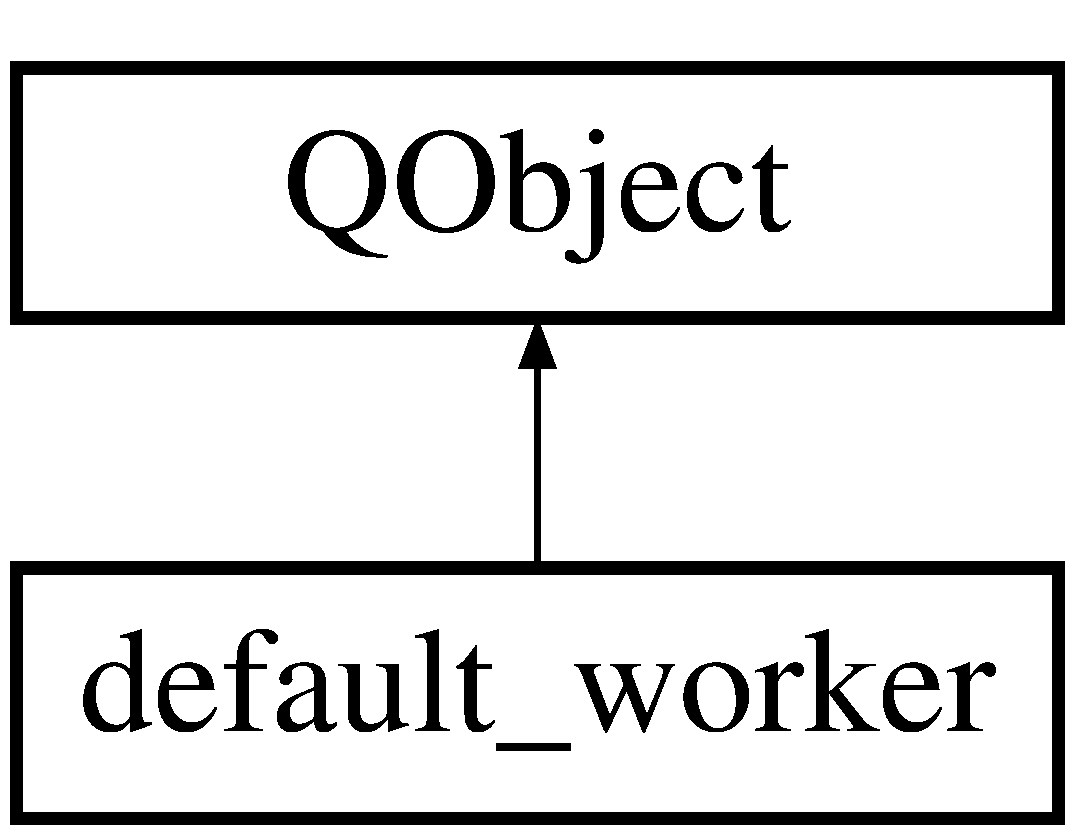
\includegraphics[height=2.000000cm]{classdefault__worker}
\end{center}
\end{figure}
\subsection*{Public Member Functions}
\begin{DoxyCompactItemize}
\item 
\hyperlink{classdefault__worker_a7c7de24d48b778cbbfaab029152523e4}{default\-\_\-worker} ()
\end{DoxyCompactItemize}
\subsection*{Private Slots}
\begin{DoxyCompactItemize}
\item 
void \hyperlink{classdefault__worker_ad24b13f13fa8c36339c7a7cef535d8b9}{test\-\_\-can\-Be\-Placed\-On\-Tile\-\_\-same\-\_\-owner} ()
\begin{DoxyCompactList}\small\item\em Tests whether an object with the same owner \par
 can be placed on a tile. \end{DoxyCompactList}\item 
void \hyperlink{classdefault__worker_a0e5d2687739d821e3f6beaa7c4e65cd9}{test\-\_\-can\-Be\-Placed\-On\-Tile\-\_\-ownerconflict} ()
\begin{DoxyCompactList}\small\item\em Tests whether an object with a different owner \par
 can be placed on a tile. \end{DoxyCompactList}\item 
void \hyperlink{classdefault__worker_a7858f59a97e1747ee452f34ffe4703ca}{test\-\_\-can\-Be\-Placed\-On\-Tile\-\_\-no\-\_\-owners} ()
\begin{DoxyCompactList}\small\item\em Tests whether an object with no owner \par
 can be placed on a tile without an owner. \end{DoxyCompactList}\item 
void \hyperlink{classdefault__worker_a2b396d92740880572f56bbab7ad584b4}{test\-\_\-set\-Location\-Tile} ()
\begin{DoxyCompactList}\small\item\em Tests whether an object can be placed on a tile. \end{DoxyCompactList}\item 
void \hyperlink{classdefault__worker_a79930b71a5ed3d6322aaa1123fbec92b}{test\-\_\-unset\-Location\-Tile} ()
\begin{DoxyCompactList}\small\item\em Tests whether an object's location can be removed. \end{DoxyCompactList}\item 
void \hyperlink{classdefault__worker_afc31832f2490e8f4099e6460a5b533ce}{test\-\_\-set\-Location\-Tile\-\_\-exception} ()
\begin{DoxyCompactList}\small\item\em Tests whether an object's location can set to a tile \par
with a different owner. \end{DoxyCompactList}\item 
void \hyperlink{classdefault__worker_a18fa8ce0183ee7fa9d39918c3ee72c6d}{test\-\_\-current\-Location\-Tile\-\_\-expired\-\_\-ptr} ()
\begin{DoxyCompactList}\small\item\em Tests whether an objects location gets removed if the \par
tile expires it was located on. \end{DoxyCompactList}\item 
void \hyperlink{classdefault__worker_a9faf7bd43cb6b07f2be5fbe16ba9c11e}{test\-\_\-tile\-Work\-Action} ()
\begin{DoxyCompactList}\small\item\em Tests worker's tileworkaction (generating resources) \end{DoxyCompactList}\item 
void \hyperlink{classdefault__worker_a130375f5e40f7c8cc24c2da1d0039b3c}{test\-\_\-tile\-Work\-Action\-\_\-not\-Enough\-Money\-And\-Food} ()
\begin{DoxyCompactList}\small\item\em Tests worker's tileworkaction when there aren't \par
enough resources. \end{DoxyCompactList}\item 
void \hyperlink{classdefault__worker_aa23fa13744f7dbfb7a8d6b3f46402b15}{test\-\_\-type\-\_\-basicworker} ()
\begin{DoxyCompactList}\small\item\em Tests Basic\-Worker's type. \end{DoxyCompactList}\item 
void \hyperlink{classdefault__worker_a18bed647358defe17331e70a024bfc61}{test\-\_\-type\-\_\-mineworker} ()
\begin{DoxyCompactList}\small\item\em Tests Mine\-Worker's type. \end{DoxyCompactList}\item 
void \hyperlink{classdefault__worker_a54075e0089e64d81493a9462de924457}{test\-\_\-type\-\_\-sawmillworker} ()
\begin{DoxyCompactList}\small\item\em Tests Saw\-Mill\-Worker's type. \end{DoxyCompactList}\item 
void \hyperlink{classdefault__worker_ac24a55220859638040a6cad7107b044f}{cleanup} ()
\begin{DoxyCompactList}\small\item\em Test cleanup. \end{DoxyCompactList}\end{DoxyCompactItemize}
\subsection*{Private Attributes}
\begin{DoxyCompactItemize}
\item 
std\-::shared\-\_\-ptr$<$ \hyperlink{classGame_1_1ObjectManager}{Object\-Manager} $>$ \hyperlink{classdefault__worker_af5dedfd6c8224ee5ca2eba1290f7a853}{obj\-Man}
\item 
std\-::shared\-\_\-ptr$<$ \hyperlink{classGame_1_1GameEventHandler}{Game\-Event\-Handler} $>$ \hyperlink{classdefault__worker_a44df0b6b6c93b3992dfbc912001c47d1}{G\-E\-Hand}
\item 
\hyperlink{namespaceCourse_ab9a46ed9cd00485e318e5731ea2f78d9}{Course\-::\-Resource\-Map} \hyperlink{classdefault__worker_acd1ecdadb65e25b996f64a42790f83d1}{start\-Resources}
\item 
std\-::shared\-\_\-ptr$<$ \hyperlink{classGame_1_1Player}{Player} $>$ \hyperlink{classdefault__worker_aba0535cd3653d51e44437df2796edb0a}{player1}
\item 
std\-::shared\-\_\-ptr$<$ \hyperlink{classGame_1_1Player}{Player} $>$ \hyperlink{classdefault__worker_a099ddc74e55afb29982086d62063e34c}{player2}
\item 
std\-::shared\-\_\-ptr$<$ \hyperlink{classCourse_1_1TileBase}{Course\-::\-Tile\-Base} $>$ \hyperlink{classdefault__worker_a1dca180451327fc342c5874f31dc5b34}{tile1}
\item 
std\-::shared\-\_\-ptr$<$ \hyperlink{classCourse_1_1TileBase}{Course\-::\-Tile\-Base} $>$ \hyperlink{classdefault__worker_a58ff3b99ca13fb2bac484383cb97224e}{tile2}
\item 
std\-::shared\-\_\-ptr$<$ \hyperlink{classCourse_1_1TileBase}{Course\-::\-Tile\-Base} $>$ \hyperlink{classdefault__worker_ae85c6a01155685fe642e8e6c55116da2}{tile\-Expire}
\item 
const \hyperlink{classCourse_1_1Coordinate}{Course\-::\-Coordinate} \hyperlink{classdefault__worker_a8d151cfc7d0d347577cdb66f3db280b0}{tile1\-\_\-coordinate} = \{1,1\}
\item 
const \hyperlink{classCourse_1_1Coordinate}{Course\-::\-Coordinate} \hyperlink{classdefault__worker_a5bbce973c2c9387484b709d57f718054}{tile2\-\_\-coordinate} = \{1,2\}
\item 
const \hyperlink{classCourse_1_1Coordinate}{Course\-::\-Coordinate} \hyperlink{classdefault__worker_a0a0fe24881186dbb4704e66f121dfeb2}{tile\-Expire\-\_\-coordinate} = \{2,2\}
\item 
std\-::shared\-\_\-ptr\\*
$<$ \hyperlink{classCourse_1_1BasicWorker}{Course\-::\-Basic\-Worker} $>$ \hyperlink{classdefault__worker_a872779c575aa3b978bd368c9c120982f}{default\-\_\-object}
\item 
std\-::shared\-\_\-ptr$<$ \hyperlink{classGame_1_1SawMillWorker}{Saw\-Mill\-Worker} $>$ \hyperlink{classdefault__worker_a266e28b4c12c4312b616acae5911bb51}{sawmillworker\-\_\-object}
\item 
std\-::shared\-\_\-ptr$<$ \hyperlink{classGame_1_1MineWorker}{Mine\-Worker} $>$ \hyperlink{classdefault__worker_a4e2482621b6bdd379211cc71006501ad}{mineworker\-\_\-object}
\end{DoxyCompactItemize}


\subsection{Detailed Description}
The worker\-\_\-tests test the Placeable\-Game\-Object and all Worker classes. 

\subsection{Constructor \& Destructor Documentation}
\hypertarget{classdefault__worker_a7c7de24d48b778cbbfaab029152523e4}{\index{default\-\_\-worker@{default\-\_\-worker}!default\-\_\-worker@{default\-\_\-worker}}
\index{default\-\_\-worker@{default\-\_\-worker}!default_worker@{default\-\_\-worker}}
\subsubsection[{default\-\_\-worker}]{\setlength{\rightskip}{0pt plus 5cm}default\-\_\-worker\-::default\-\_\-worker (
\begin{DoxyParamCaption}
{}
\end{DoxyParamCaption}
)}}\label{classdefault__worker_a7c7de24d48b778cbbfaab029152523e4}


\subsection{Member Function Documentation}
\hypertarget{classdefault__worker_ac24a55220859638040a6cad7107b044f}{\index{default\-\_\-worker@{default\-\_\-worker}!cleanup@{cleanup}}
\index{cleanup@{cleanup}!default_worker@{default\-\_\-worker}}
\subsubsection[{cleanup}]{\setlength{\rightskip}{0pt plus 5cm}void default\-\_\-worker\-::cleanup (
\begin{DoxyParamCaption}
{}
\end{DoxyParamCaption}
)\hspace{0.3cm}{\ttfamily [private]}, {\ttfamily [slot]}}}\label{classdefault__worker_ac24a55220859638040a6cad7107b044f}


Test cleanup. 

\hypertarget{classdefault__worker_a7858f59a97e1747ee452f34ffe4703ca}{\index{default\-\_\-worker@{default\-\_\-worker}!test\-\_\-can\-Be\-Placed\-On\-Tile\-\_\-no\-\_\-owners@{test\-\_\-can\-Be\-Placed\-On\-Tile\-\_\-no\-\_\-owners}}
\index{test\-\_\-can\-Be\-Placed\-On\-Tile\-\_\-no\-\_\-owners@{test\-\_\-can\-Be\-Placed\-On\-Tile\-\_\-no\-\_\-owners}!default_worker@{default\-\_\-worker}}
\subsubsection[{test\-\_\-can\-Be\-Placed\-On\-Tile\-\_\-no\-\_\-owners}]{\setlength{\rightskip}{0pt plus 5cm}void default\-\_\-worker\-::test\-\_\-can\-Be\-Placed\-On\-Tile\-\_\-no\-\_\-owners (
\begin{DoxyParamCaption}
{}
\end{DoxyParamCaption}
)\hspace{0.3cm}{\ttfamily [private]}, {\ttfamily [slot]}}}\label{classdefault__worker_a7858f59a97e1747ee452f34ffe4703ca}


Tests whether an object with no owner \par
 can be placed on a tile without an owner. 

\begin{DoxyPostcond}{Postcondition}
Should be possible 
\end{DoxyPostcond}
\hypertarget{classdefault__worker_a0e5d2687739d821e3f6beaa7c4e65cd9}{\index{default\-\_\-worker@{default\-\_\-worker}!test\-\_\-can\-Be\-Placed\-On\-Tile\-\_\-ownerconflict@{test\-\_\-can\-Be\-Placed\-On\-Tile\-\_\-ownerconflict}}
\index{test\-\_\-can\-Be\-Placed\-On\-Tile\-\_\-ownerconflict@{test\-\_\-can\-Be\-Placed\-On\-Tile\-\_\-ownerconflict}!default_worker@{default\-\_\-worker}}
\subsubsection[{test\-\_\-can\-Be\-Placed\-On\-Tile\-\_\-ownerconflict}]{\setlength{\rightskip}{0pt plus 5cm}void default\-\_\-worker\-::test\-\_\-can\-Be\-Placed\-On\-Tile\-\_\-ownerconflict (
\begin{DoxyParamCaption}
{}
\end{DoxyParamCaption}
)\hspace{0.3cm}{\ttfamily [private]}, {\ttfamily [slot]}}}\label{classdefault__worker_a0e5d2687739d821e3f6beaa7c4e65cd9}


Tests whether an object with a different owner \par
 can be placed on a tile. 

\begin{DoxyPostcond}{Postcondition}
Should not be possible 
\end{DoxyPostcond}
\hypertarget{classdefault__worker_ad24b13f13fa8c36339c7a7cef535d8b9}{\index{default\-\_\-worker@{default\-\_\-worker}!test\-\_\-can\-Be\-Placed\-On\-Tile\-\_\-same\-\_\-owner@{test\-\_\-can\-Be\-Placed\-On\-Tile\-\_\-same\-\_\-owner}}
\index{test\-\_\-can\-Be\-Placed\-On\-Tile\-\_\-same\-\_\-owner@{test\-\_\-can\-Be\-Placed\-On\-Tile\-\_\-same\-\_\-owner}!default_worker@{default\-\_\-worker}}
\subsubsection[{test\-\_\-can\-Be\-Placed\-On\-Tile\-\_\-same\-\_\-owner}]{\setlength{\rightskip}{0pt plus 5cm}void default\-\_\-worker\-::test\-\_\-can\-Be\-Placed\-On\-Tile\-\_\-same\-\_\-owner (
\begin{DoxyParamCaption}
{}
\end{DoxyParamCaption}
)\hspace{0.3cm}{\ttfamily [private]}, {\ttfamily [slot]}}}\label{classdefault__worker_ad24b13f13fa8c36339c7a7cef535d8b9}


Tests whether an object with the same owner \par
 can be placed on a tile. 

\begin{DoxyPostcond}{Postcondition}
Should be possible 
\end{DoxyPostcond}
\hypertarget{classdefault__worker_a18fa8ce0183ee7fa9d39918c3ee72c6d}{\index{default\-\_\-worker@{default\-\_\-worker}!test\-\_\-current\-Location\-Tile\-\_\-expired\-\_\-ptr@{test\-\_\-current\-Location\-Tile\-\_\-expired\-\_\-ptr}}
\index{test\-\_\-current\-Location\-Tile\-\_\-expired\-\_\-ptr@{test\-\_\-current\-Location\-Tile\-\_\-expired\-\_\-ptr}!default_worker@{default\-\_\-worker}}
\subsubsection[{test\-\_\-current\-Location\-Tile\-\_\-expired\-\_\-ptr}]{\setlength{\rightskip}{0pt plus 5cm}void default\-\_\-worker\-::test\-\_\-current\-Location\-Tile\-\_\-expired\-\_\-ptr (
\begin{DoxyParamCaption}
{}
\end{DoxyParamCaption}
)\hspace{0.3cm}{\ttfamily [private]}, {\ttfamily [slot]}}}\label{classdefault__worker_a18fa8ce0183ee7fa9d39918c3ee72c6d}


Tests whether an objects location gets removed if the \par
tile expires it was located on. 

\begin{DoxyPostcond}{Postcondition}
Should be removed 
\end{DoxyPostcond}
\hypertarget{classdefault__worker_a2b396d92740880572f56bbab7ad584b4}{\index{default\-\_\-worker@{default\-\_\-worker}!test\-\_\-set\-Location\-Tile@{test\-\_\-set\-Location\-Tile}}
\index{test\-\_\-set\-Location\-Tile@{test\-\_\-set\-Location\-Tile}!default_worker@{default\-\_\-worker}}
\subsubsection[{test\-\_\-set\-Location\-Tile}]{\setlength{\rightskip}{0pt plus 5cm}void default\-\_\-worker\-::test\-\_\-set\-Location\-Tile (
\begin{DoxyParamCaption}
{}
\end{DoxyParamCaption}
)\hspace{0.3cm}{\ttfamily [private]}, {\ttfamily [slot]}}}\label{classdefault__worker_a2b396d92740880572f56bbab7ad584b4}


Tests whether an object can be placed on a tile. 

\begin{DoxyPostcond}{Postcondition}
Should be possible 
\end{DoxyPostcond}
\hypertarget{classdefault__worker_afc31832f2490e8f4099e6460a5b533ce}{\index{default\-\_\-worker@{default\-\_\-worker}!test\-\_\-set\-Location\-Tile\-\_\-exception@{test\-\_\-set\-Location\-Tile\-\_\-exception}}
\index{test\-\_\-set\-Location\-Tile\-\_\-exception@{test\-\_\-set\-Location\-Tile\-\_\-exception}!default_worker@{default\-\_\-worker}}
\subsubsection[{test\-\_\-set\-Location\-Tile\-\_\-exception}]{\setlength{\rightskip}{0pt plus 5cm}void default\-\_\-worker\-::test\-\_\-set\-Location\-Tile\-\_\-exception (
\begin{DoxyParamCaption}
{}
\end{DoxyParamCaption}
)\hspace{0.3cm}{\ttfamily [private]}, {\ttfamily [slot]}}}\label{classdefault__worker_afc31832f2490e8f4099e6460a5b533ce}


Tests whether an object's location can set to a tile \par
with a different owner. 

\begin{DoxyPostcond}{Postcondition}
Should throw an Illegal\-Action exception 
\end{DoxyPostcond}
\hypertarget{classdefault__worker_a9faf7bd43cb6b07f2be5fbe16ba9c11e}{\index{default\-\_\-worker@{default\-\_\-worker}!test\-\_\-tile\-Work\-Action@{test\-\_\-tile\-Work\-Action}}
\index{test\-\_\-tile\-Work\-Action@{test\-\_\-tile\-Work\-Action}!default_worker@{default\-\_\-worker}}
\subsubsection[{test\-\_\-tile\-Work\-Action}]{\setlength{\rightskip}{0pt plus 5cm}void default\-\_\-worker\-::test\-\_\-tile\-Work\-Action (
\begin{DoxyParamCaption}
{}
\end{DoxyParamCaption}
)\hspace{0.3cm}{\ttfamily [private]}, {\ttfamily [slot]}}}\label{classdefault__worker_a9faf7bd43cb6b07f2be5fbe16ba9c11e}


Tests worker's tileworkaction (generating resources) 

\begin{DoxyPostcond}{Postcondition}
Should generate resources 
\end{DoxyPostcond}
\hypertarget{classdefault__worker_a130375f5e40f7c8cc24c2da1d0039b3c}{\index{default\-\_\-worker@{default\-\_\-worker}!test\-\_\-tile\-Work\-Action\-\_\-not\-Enough\-Money\-And\-Food@{test\-\_\-tile\-Work\-Action\-\_\-not\-Enough\-Money\-And\-Food}}
\index{test\-\_\-tile\-Work\-Action\-\_\-not\-Enough\-Money\-And\-Food@{test\-\_\-tile\-Work\-Action\-\_\-not\-Enough\-Money\-And\-Food}!default_worker@{default\-\_\-worker}}
\subsubsection[{test\-\_\-tile\-Work\-Action\-\_\-not\-Enough\-Money\-And\-Food}]{\setlength{\rightskip}{0pt plus 5cm}void default\-\_\-worker\-::test\-\_\-tile\-Work\-Action\-\_\-not\-Enough\-Money\-And\-Food (
\begin{DoxyParamCaption}
{}
\end{DoxyParamCaption}
)\hspace{0.3cm}{\ttfamily [private]}, {\ttfamily [slot]}}}\label{classdefault__worker_a130375f5e40f7c8cc24c2da1d0039b3c}


Tests worker's tileworkaction when there aren't \par
enough resources. 

\begin{DoxyPostcond}{Postcondition}
Should not give resources 
\end{DoxyPostcond}
\hypertarget{classdefault__worker_aa23fa13744f7dbfb7a8d6b3f46402b15}{\index{default\-\_\-worker@{default\-\_\-worker}!test\-\_\-type\-\_\-basicworker@{test\-\_\-type\-\_\-basicworker}}
\index{test\-\_\-type\-\_\-basicworker@{test\-\_\-type\-\_\-basicworker}!default_worker@{default\-\_\-worker}}
\subsubsection[{test\-\_\-type\-\_\-basicworker}]{\setlength{\rightskip}{0pt plus 5cm}void default\-\_\-worker\-::test\-\_\-type\-\_\-basicworker (
\begin{DoxyParamCaption}
{}
\end{DoxyParamCaption}
)\hspace{0.3cm}{\ttfamily [private]}, {\ttfamily [slot]}}}\label{classdefault__worker_aa23fa13744f7dbfb7a8d6b3f46402b15}


Tests Basic\-Worker's type. 

\begin{DoxyPostcond}{Postcondition}
Should be Basic\-Worker 
\end{DoxyPostcond}
\hypertarget{classdefault__worker_a18bed647358defe17331e70a024bfc61}{\index{default\-\_\-worker@{default\-\_\-worker}!test\-\_\-type\-\_\-mineworker@{test\-\_\-type\-\_\-mineworker}}
\index{test\-\_\-type\-\_\-mineworker@{test\-\_\-type\-\_\-mineworker}!default_worker@{default\-\_\-worker}}
\subsubsection[{test\-\_\-type\-\_\-mineworker}]{\setlength{\rightskip}{0pt plus 5cm}void default\-\_\-worker\-::test\-\_\-type\-\_\-mineworker (
\begin{DoxyParamCaption}
{}
\end{DoxyParamCaption}
)\hspace{0.3cm}{\ttfamily [private]}, {\ttfamily [slot]}}}\label{classdefault__worker_a18bed647358defe17331e70a024bfc61}


Tests Mine\-Worker's type. 

\begin{DoxyPostcond}{Postcondition}
Should be Mine\-Worker 
\end{DoxyPostcond}
\hypertarget{classdefault__worker_a54075e0089e64d81493a9462de924457}{\index{default\-\_\-worker@{default\-\_\-worker}!test\-\_\-type\-\_\-sawmillworker@{test\-\_\-type\-\_\-sawmillworker}}
\index{test\-\_\-type\-\_\-sawmillworker@{test\-\_\-type\-\_\-sawmillworker}!default_worker@{default\-\_\-worker}}
\subsubsection[{test\-\_\-type\-\_\-sawmillworker}]{\setlength{\rightskip}{0pt plus 5cm}void default\-\_\-worker\-::test\-\_\-type\-\_\-sawmillworker (
\begin{DoxyParamCaption}
{}
\end{DoxyParamCaption}
)\hspace{0.3cm}{\ttfamily [private]}, {\ttfamily [slot]}}}\label{classdefault__worker_a54075e0089e64d81493a9462de924457}


Tests Saw\-Mill\-Worker's type. 

\begin{DoxyPostcond}{Postcondition}
Should be Saw\-Mill\-Worker 
\end{DoxyPostcond}
\hypertarget{classdefault__worker_a79930b71a5ed3d6322aaa1123fbec92b}{\index{default\-\_\-worker@{default\-\_\-worker}!test\-\_\-unset\-Location\-Tile@{test\-\_\-unset\-Location\-Tile}}
\index{test\-\_\-unset\-Location\-Tile@{test\-\_\-unset\-Location\-Tile}!default_worker@{default\-\_\-worker}}
\subsubsection[{test\-\_\-unset\-Location\-Tile}]{\setlength{\rightskip}{0pt plus 5cm}void default\-\_\-worker\-::test\-\_\-unset\-Location\-Tile (
\begin{DoxyParamCaption}
{}
\end{DoxyParamCaption}
)\hspace{0.3cm}{\ttfamily [private]}, {\ttfamily [slot]}}}\label{classdefault__worker_a79930b71a5ed3d6322aaa1123fbec92b}


Tests whether an object's location can be removed. 

\begin{DoxyPostcond}{Postcondition}
Should be possible 
\end{DoxyPostcond}


\subsection{Member Data Documentation}
\hypertarget{classdefault__worker_a872779c575aa3b978bd368c9c120982f}{\index{default\-\_\-worker@{default\-\_\-worker}!default\-\_\-object@{default\-\_\-object}}
\index{default\-\_\-object@{default\-\_\-object}!default_worker@{default\-\_\-worker}}
\subsubsection[{default\-\_\-object}]{\setlength{\rightskip}{0pt plus 5cm}std\-::shared\-\_\-ptr$<${\bf Course\-::\-Basic\-Worker}$>$ default\-\_\-worker\-::default\-\_\-object\hspace{0.3cm}{\ttfamily [private]}}}\label{classdefault__worker_a872779c575aa3b978bd368c9c120982f}
\hypertarget{classdefault__worker_a44df0b6b6c93b3992dfbc912001c47d1}{\index{default\-\_\-worker@{default\-\_\-worker}!G\-E\-Hand@{G\-E\-Hand}}
\index{G\-E\-Hand@{G\-E\-Hand}!default_worker@{default\-\_\-worker}}
\subsubsection[{G\-E\-Hand}]{\setlength{\rightskip}{0pt plus 5cm}std\-::shared\-\_\-ptr$<${\bf Game\-Event\-Handler}$>$ default\-\_\-worker\-::\-G\-E\-Hand\hspace{0.3cm}{\ttfamily [private]}}}\label{classdefault__worker_a44df0b6b6c93b3992dfbc912001c47d1}
\hypertarget{classdefault__worker_a4e2482621b6bdd379211cc71006501ad}{\index{default\-\_\-worker@{default\-\_\-worker}!mineworker\-\_\-object@{mineworker\-\_\-object}}
\index{mineworker\-\_\-object@{mineworker\-\_\-object}!default_worker@{default\-\_\-worker}}
\subsubsection[{mineworker\-\_\-object}]{\setlength{\rightskip}{0pt plus 5cm}std\-::shared\-\_\-ptr$<${\bf Mine\-Worker}$>$ default\-\_\-worker\-::mineworker\-\_\-object\hspace{0.3cm}{\ttfamily [private]}}}\label{classdefault__worker_a4e2482621b6bdd379211cc71006501ad}
\hypertarget{classdefault__worker_af5dedfd6c8224ee5ca2eba1290f7a853}{\index{default\-\_\-worker@{default\-\_\-worker}!obj\-Man@{obj\-Man}}
\index{obj\-Man@{obj\-Man}!default_worker@{default\-\_\-worker}}
\subsubsection[{obj\-Man}]{\setlength{\rightskip}{0pt plus 5cm}std\-::shared\-\_\-ptr$<${\bf Object\-Manager}$>$ default\-\_\-worker\-::obj\-Man\hspace{0.3cm}{\ttfamily [private]}}}\label{classdefault__worker_af5dedfd6c8224ee5ca2eba1290f7a853}
\hypertarget{classdefault__worker_aba0535cd3653d51e44437df2796edb0a}{\index{default\-\_\-worker@{default\-\_\-worker}!player1@{player1}}
\index{player1@{player1}!default_worker@{default\-\_\-worker}}
\subsubsection[{player1}]{\setlength{\rightskip}{0pt plus 5cm}std\-::shared\-\_\-ptr$<${\bf Player}$>$ default\-\_\-worker\-::player1\hspace{0.3cm}{\ttfamily [private]}}}\label{classdefault__worker_aba0535cd3653d51e44437df2796edb0a}
\hypertarget{classdefault__worker_a099ddc74e55afb29982086d62063e34c}{\index{default\-\_\-worker@{default\-\_\-worker}!player2@{player2}}
\index{player2@{player2}!default_worker@{default\-\_\-worker}}
\subsubsection[{player2}]{\setlength{\rightskip}{0pt plus 5cm}std\-::shared\-\_\-ptr$<${\bf Player}$>$ default\-\_\-worker\-::player2\hspace{0.3cm}{\ttfamily [private]}}}\label{classdefault__worker_a099ddc74e55afb29982086d62063e34c}
\hypertarget{classdefault__worker_a266e28b4c12c4312b616acae5911bb51}{\index{default\-\_\-worker@{default\-\_\-worker}!sawmillworker\-\_\-object@{sawmillworker\-\_\-object}}
\index{sawmillworker\-\_\-object@{sawmillworker\-\_\-object}!default_worker@{default\-\_\-worker}}
\subsubsection[{sawmillworker\-\_\-object}]{\setlength{\rightskip}{0pt plus 5cm}std\-::shared\-\_\-ptr$<${\bf Saw\-Mill\-Worker}$>$ default\-\_\-worker\-::sawmillworker\-\_\-object\hspace{0.3cm}{\ttfamily [private]}}}\label{classdefault__worker_a266e28b4c12c4312b616acae5911bb51}
\hypertarget{classdefault__worker_acd1ecdadb65e25b996f64a42790f83d1}{\index{default\-\_\-worker@{default\-\_\-worker}!start\-Resources@{start\-Resources}}
\index{start\-Resources@{start\-Resources}!default_worker@{default\-\_\-worker}}
\subsubsection[{start\-Resources}]{\setlength{\rightskip}{0pt plus 5cm}{\bf Course\-::\-Resource\-Map} default\-\_\-worker\-::start\-Resources\hspace{0.3cm}{\ttfamily [private]}}}\label{classdefault__worker_acd1ecdadb65e25b996f64a42790f83d1}
\hypertarget{classdefault__worker_a1dca180451327fc342c5874f31dc5b34}{\index{default\-\_\-worker@{default\-\_\-worker}!tile1@{tile1}}
\index{tile1@{tile1}!default_worker@{default\-\_\-worker}}
\subsubsection[{tile1}]{\setlength{\rightskip}{0pt plus 5cm}std\-::shared\-\_\-ptr$<${\bf Course\-::\-Tile\-Base}$>$ default\-\_\-worker\-::tile1\hspace{0.3cm}{\ttfamily [private]}}}\label{classdefault__worker_a1dca180451327fc342c5874f31dc5b34}
\hypertarget{classdefault__worker_a8d151cfc7d0d347577cdb66f3db280b0}{\index{default\-\_\-worker@{default\-\_\-worker}!tile1\-\_\-coordinate@{tile1\-\_\-coordinate}}
\index{tile1\-\_\-coordinate@{tile1\-\_\-coordinate}!default_worker@{default\-\_\-worker}}
\subsubsection[{tile1\-\_\-coordinate}]{\setlength{\rightskip}{0pt plus 5cm}const {\bf Course\-::\-Coordinate} default\-\_\-worker\-::tile1\-\_\-coordinate = \{1,1\}\hspace{0.3cm}{\ttfamily [private]}}}\label{classdefault__worker_a8d151cfc7d0d347577cdb66f3db280b0}
\hypertarget{classdefault__worker_a58ff3b99ca13fb2bac484383cb97224e}{\index{default\-\_\-worker@{default\-\_\-worker}!tile2@{tile2}}
\index{tile2@{tile2}!default_worker@{default\-\_\-worker}}
\subsubsection[{tile2}]{\setlength{\rightskip}{0pt plus 5cm}std\-::shared\-\_\-ptr$<${\bf Course\-::\-Tile\-Base}$>$ default\-\_\-worker\-::tile2\hspace{0.3cm}{\ttfamily [private]}}}\label{classdefault__worker_a58ff3b99ca13fb2bac484383cb97224e}
\hypertarget{classdefault__worker_a5bbce973c2c9387484b709d57f718054}{\index{default\-\_\-worker@{default\-\_\-worker}!tile2\-\_\-coordinate@{tile2\-\_\-coordinate}}
\index{tile2\-\_\-coordinate@{tile2\-\_\-coordinate}!default_worker@{default\-\_\-worker}}
\subsubsection[{tile2\-\_\-coordinate}]{\setlength{\rightskip}{0pt plus 5cm}const {\bf Course\-::\-Coordinate} default\-\_\-worker\-::tile2\-\_\-coordinate = \{1,2\}\hspace{0.3cm}{\ttfamily [private]}}}\label{classdefault__worker_a5bbce973c2c9387484b709d57f718054}
\hypertarget{classdefault__worker_ae85c6a01155685fe642e8e6c55116da2}{\index{default\-\_\-worker@{default\-\_\-worker}!tile\-Expire@{tile\-Expire}}
\index{tile\-Expire@{tile\-Expire}!default_worker@{default\-\_\-worker}}
\subsubsection[{tile\-Expire}]{\setlength{\rightskip}{0pt plus 5cm}std\-::shared\-\_\-ptr$<${\bf Course\-::\-Tile\-Base}$>$ default\-\_\-worker\-::tile\-Expire\hspace{0.3cm}{\ttfamily [private]}}}\label{classdefault__worker_ae85c6a01155685fe642e8e6c55116da2}
\hypertarget{classdefault__worker_a0a0fe24881186dbb4704e66f121dfeb2}{\index{default\-\_\-worker@{default\-\_\-worker}!tile\-Expire\-\_\-coordinate@{tile\-Expire\-\_\-coordinate}}
\index{tile\-Expire\-\_\-coordinate@{tile\-Expire\-\_\-coordinate}!default_worker@{default\-\_\-worker}}
\subsubsection[{tile\-Expire\-\_\-coordinate}]{\setlength{\rightskip}{0pt plus 5cm}const {\bf Course\-::\-Coordinate} default\-\_\-worker\-::tile\-Expire\-\_\-coordinate = \{2,2\}\hspace{0.3cm}{\ttfamily [private]}}}\label{classdefault__worker_a0a0fe24881186dbb4704e66f121dfeb2}


The documentation for this class was generated from the following file\-:\begin{DoxyCompactItemize}
\item 
Unit\-Tests/worker\-\_\-tests/\hyperlink{tst__default__worker_8cpp}{tst\-\_\-default\-\_\-worker.\-cpp}\end{DoxyCompactItemize}

\hypertarget{classenddialog}{\section{enddialog Class Reference}
\label{classenddialog}\index{enddialog@{enddialog}}
}


The enddialog class shows pop-\/up window announcing the result when game ends.  




{\ttfamily \#include $<$enddialog.\-hh$>$}

Inheritance diagram for enddialog\-:\begin{figure}[H]
\begin{center}
\leavevmode
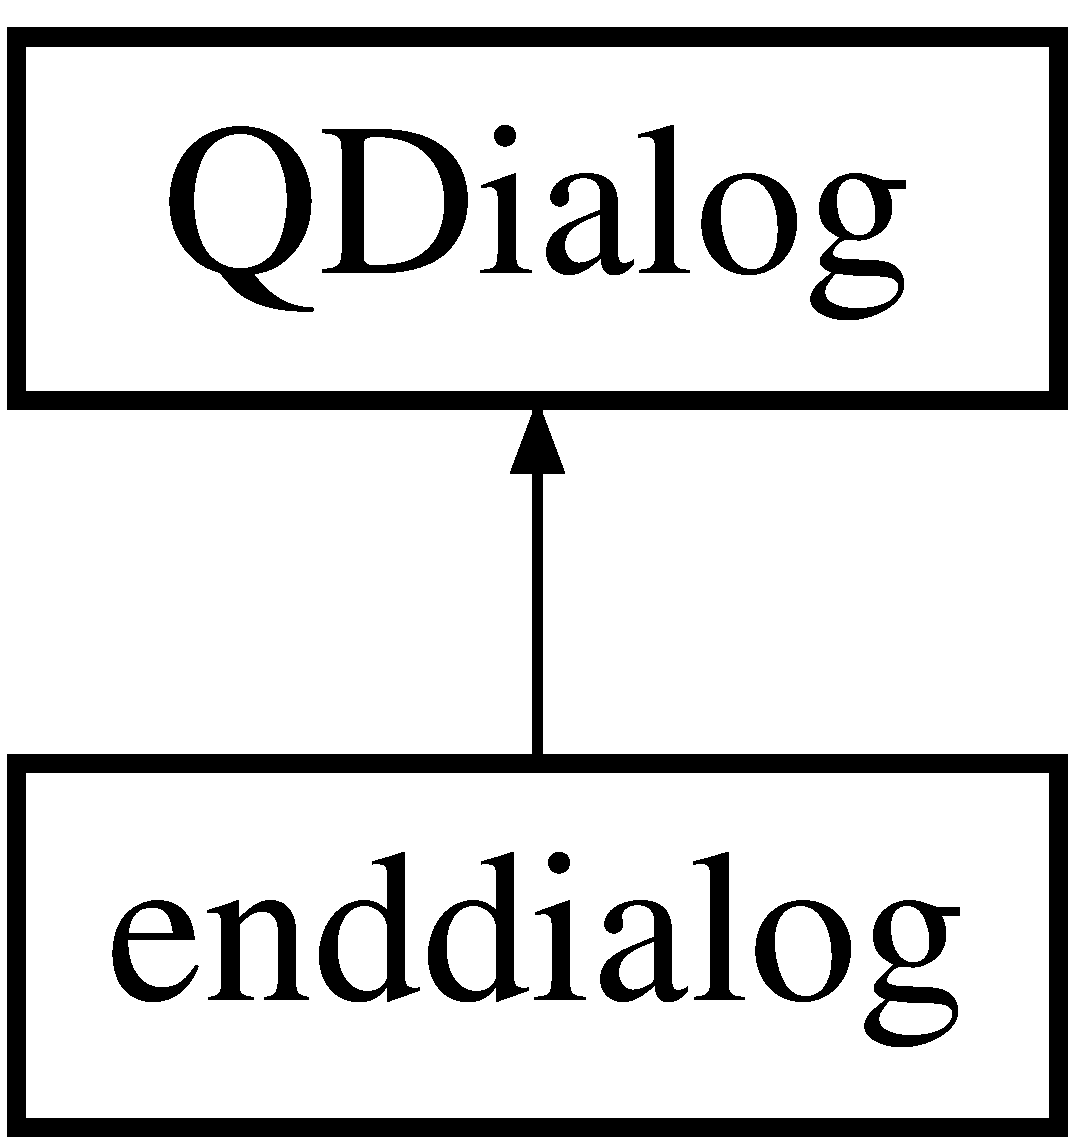
\includegraphics[height=2.000000cm]{classenddialog}
\end{center}
\end{figure}
\subsection*{Public Member Functions}
\begin{DoxyCompactItemize}
\item 
\hyperlink{classenddialog_a5dcbc64678b43043e16f74bd4c4dffb0}{enddialog} (Q\-Widget $\ast$parent=0)
\begin{DoxyCompactList}\small\item\em Constructor for the class. \end{DoxyCompactList}\item 
void \hyperlink{classenddialog_ab3da4bfad75f08deb94a5139799fcbb9}{set\-Winner} (std\-::vector$<$ std\-::shared\-\_\-ptr$<$ \hyperlink{classPlayer}{Player} $>$ $>$ winners, int round)
\begin{DoxyCompactList}\small\item\em set\-Winner Announces winner or a draw in the end of the game. \end{DoxyCompactList}\end{DoxyCompactItemize}


\subsection{Detailed Description}
The enddialog class shows pop-\/up window announcing the result when game ends. 

Has text label for game result and exit button for quitting the game. 

\subsection{Constructor \& Destructor Documentation}
\hypertarget{classenddialog_a5dcbc64678b43043e16f74bd4c4dffb0}{\index{enddialog@{enddialog}!enddialog@{enddialog}}
\index{enddialog@{enddialog}!enddialog@{enddialog}}
\subsubsection[{enddialog}]{\setlength{\rightskip}{0pt plus 5cm}enddialog\-::enddialog (
\begin{DoxyParamCaption}
\item[{Q\-Widget $\ast$}]{parent = {\ttfamily 0}}
\end{DoxyParamCaption}
)\hspace{0.3cm}{\ttfamily [explicit]}}}\label{classenddialog_a5dcbc64678b43043e16f74bd4c4dffb0}


Constructor for the class. 


\begin{DoxyParams}{Parameters}
{\em parent} & can be used to point to a parent widget. Not used. \\
\hline
\end{DoxyParams}


\subsection{Member Function Documentation}
\hypertarget{classenddialog_ab3da4bfad75f08deb94a5139799fcbb9}{\index{enddialog@{enddialog}!set\-Winner@{set\-Winner}}
\index{set\-Winner@{set\-Winner}!enddialog@{enddialog}}
\subsubsection[{set\-Winner}]{\setlength{\rightskip}{0pt plus 5cm}void enddialog\-::set\-Winner (
\begin{DoxyParamCaption}
\item[{std\-::vector$<$ std\-::shared\-\_\-ptr$<$ {\bf Player} $>$ $>$}]{winners, }
\item[{int}]{round}
\end{DoxyParamCaption}
)}}\label{classenddialog_ab3da4bfad75f08deb94a5139799fcbb9}


set\-Winner Announces winner or a draw in the end of the game. 


\begin{DoxyParams}{Parameters}
{\em winners} & Pointer to vector which has winner or winners. \\
\hline
{\em round} & Number of rounds played. \\
\hline
\end{DoxyParams}


The documentation for this class was generated from the following files\-:\begin{DoxyCompactItemize}
\item 
enddialog.\-hh\item 
enddialog.\-cpp\end{DoxyCompactItemize}

\hypertarget{classCourse_1_1Farm}{\section{Course\-:\-:Farm Class Reference}
\label{classCourse_1_1Farm}\index{Course\-::\-Farm@{Course\-::\-Farm}}
}


The \hyperlink{classCourse_1_1Farm}{Farm} class represents a farm-\/building in the game.  




{\ttfamily \#include $<$farm.\-h$>$}

Inheritance diagram for Course\-:\-:Farm\-:\begin{figure}[H]
\begin{center}
\leavevmode
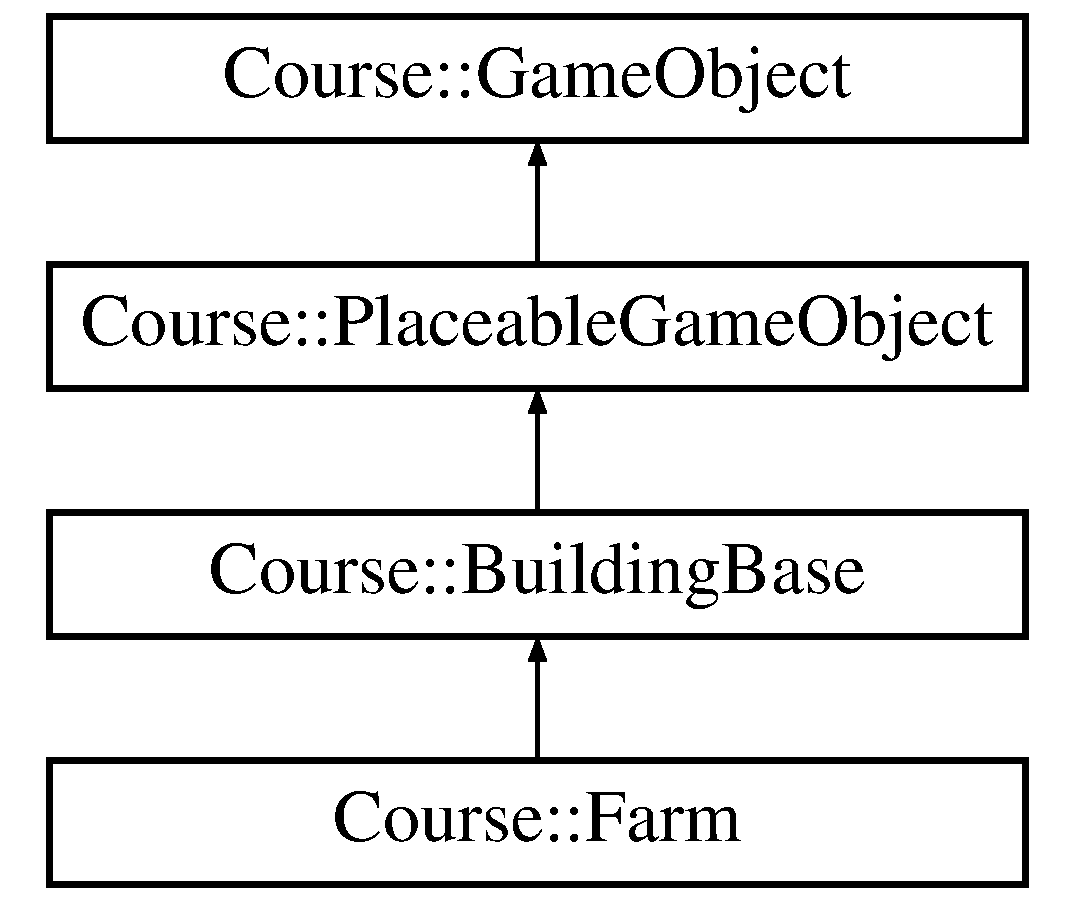
\includegraphics[height=4.000000cm]{classCourse_1_1Farm}
\end{center}
\end{figure}
\subsection*{Public Member Functions}
\begin{DoxyCompactItemize}
\item 
\hyperlink{classCourse_1_1Farm_a3b92d4bdac7e8f7fd1f648bb1a4a2490}{Farm} ()=delete
\begin{DoxyCompactList}\small\item\em Disabled parameterless constructor. \end{DoxyCompactList}\item 
\hyperlink{classCourse_1_1Farm_a01270b705f0bc18f2fc4c5c31f41cf3b}{Farm} (const std\-::shared\-\_\-ptr$<$ \hyperlink{classCourse_1_1iGameEventHandler}{i\-Game\-Event\-Handler} $>$ \&eventhandler, const std\-::shared\-\_\-ptr$<$ \hyperlink{classCourse_1_1iObjectManager}{i\-Object\-Manager} $>$ \&objectmanager, const std\-::shared\-\_\-ptr$<$ \hyperlink{classCourse_1_1PlayerBase}{Player\-Base} $>$ \&owner, const int \&tilespaces=1, const \hyperlink{namespaceCourse_ab9a46ed9cd00485e318e5731ea2f78d9}{Resource\-Map} \&buildcost=\hyperlink{namespaceCourse_1_1ConstResourceMaps_a4919571a8aa47de7c6e513de147642ef}{Const\-Resource\-Maps\-::\-F\-A\-R\-M\-\_\-\-B\-U\-I\-L\-D\-\_\-\-C\-O\-S\-T}, const \hyperlink{namespaceCourse_ab9a46ed9cd00485e318e5731ea2f78d9}{Resource\-Map} \&production=\hyperlink{namespaceCourse_1_1ConstResourceMaps_ac05142db09e7f1f85c7d936356a35df2}{Const\-Resource\-Maps\-::\-F\-A\-R\-M\-\_\-\-P\-R\-O\-D\-U\-C\-T\-I\-O\-N})
\begin{DoxyCompactList}\small\item\em Constructor for the class. \end{DoxyCompactList}\item 
virtual \hyperlink{classCourse_1_1Farm_a99c06d0eeb549a04390bd260cc7ac68d}{$\sim$\-Farm} ()=default
\begin{DoxyCompactList}\small\item\em Default destructor. \end{DoxyCompactList}\item 
virtual std\-::string \hyperlink{classCourse_1_1Farm_a54ade72809a36d31e0e426eb79d6251a}{get\-Type} () const override
\begin{DoxyCompactList}\small\item\em get\-Type Returns a string describing objects type. This should be overriden in each inherited class. Makes checking object's type easier for students. \end{DoxyCompactList}\end{DoxyCompactItemize}
\subsection*{Additional Inherited Members}


\subsection{Detailed Description}
The \hyperlink{classCourse_1_1Farm}{Farm} class represents a farm-\/building in the game. 

The farm adds 2 base-\/production for food. 

\subsection{Constructor \& Destructor Documentation}
\hypertarget{classCourse_1_1Farm_a3b92d4bdac7e8f7fd1f648bb1a4a2490}{\index{Course\-::\-Farm@{Course\-::\-Farm}!Farm@{Farm}}
\index{Farm@{Farm}!Course::Farm@{Course\-::\-Farm}}
\subsubsection[{Farm}]{\setlength{\rightskip}{0pt plus 5cm}Course\-::\-Farm\-::\-Farm (
\begin{DoxyParamCaption}
{}
\end{DoxyParamCaption}
)\hspace{0.3cm}{\ttfamily [delete]}}}\label{classCourse_1_1Farm_a3b92d4bdac7e8f7fd1f648bb1a4a2490}


Disabled parameterless constructor. 

\hypertarget{classCourse_1_1Farm_a01270b705f0bc18f2fc4c5c31f41cf3b}{\index{Course\-::\-Farm@{Course\-::\-Farm}!Farm@{Farm}}
\index{Farm@{Farm}!Course::Farm@{Course\-::\-Farm}}
\subsubsection[{Farm}]{\setlength{\rightskip}{0pt plus 5cm}Course\-::\-Farm\-::\-Farm (
\begin{DoxyParamCaption}
\item[{const std\-::shared\-\_\-ptr$<$ {\bf i\-Game\-Event\-Handler} $>$ \&}]{eventhandler, }
\item[{const std\-::shared\-\_\-ptr$<$ {\bf i\-Object\-Manager} $>$ \&}]{objectmanager, }
\item[{const std\-::shared\-\_\-ptr$<$ {\bf Player\-Base} $>$ \&}]{owner, }
\item[{const int \&}]{tilespaces = {\ttfamily 1}, }
\item[{const {\bf Resource\-Map} \&}]{buildcost = {\ttfamily {\bf Const\-Resource\-Maps\-::\-F\-A\-R\-M\-\_\-\-B\-U\-I\-L\-D\-\_\-\-C\-O\-S\-T}}, }
\item[{const {\bf Resource\-Map} \&}]{production = {\ttfamily {\bf Const\-Resource\-Maps\-::\-F\-A\-R\-M\-\_\-\-P\-R\-O\-D\-U\-C\-T\-I\-O\-N}}}
\end{DoxyParamCaption}
)\hspace{0.3cm}{\ttfamily [explicit]}}}\label{classCourse_1_1Farm_a01270b705f0bc18f2fc4c5c31f41cf3b}


Constructor for the class. 


\begin{DoxyParams}{Parameters}
{\em eventhandler} & points to the student's Game\-Event\-Handler. \\
\hline
{\em owner} & points to the owning player. \\
\hline
{\em tile} & points to the tile upon which the building is constructed.\\
\hline
\end{DoxyParams}
\begin{DoxyPostcond}{Postcondition}
Exception Guarantee\-: No guarantee. 
\end{DoxyPostcond}

\begin{DoxyExceptions}{Exceptions}
{\em \hyperlink{classCourse_1_1OwnerConflict}{Owner\-Conflict}} & -\/ if the building conflicts with tile's ownership. \\
\hline
\end{DoxyExceptions}
\hypertarget{classCourse_1_1Farm_a99c06d0eeb549a04390bd260cc7ac68d}{\index{Course\-::\-Farm@{Course\-::\-Farm}!$\sim$\-Farm@{$\sim$\-Farm}}
\index{$\sim$\-Farm@{$\sim$\-Farm}!Course::Farm@{Course\-::\-Farm}}
\subsubsection[{$\sim$\-Farm}]{\setlength{\rightskip}{0pt plus 5cm}virtual Course\-::\-Farm\-::$\sim$\-Farm (
\begin{DoxyParamCaption}
{}
\end{DoxyParamCaption}
)\hspace{0.3cm}{\ttfamily [virtual]}, {\ttfamily [default]}}}\label{classCourse_1_1Farm_a99c06d0eeb549a04390bd260cc7ac68d}


Default destructor. 



\subsection{Member Function Documentation}
\hypertarget{classCourse_1_1Farm_a54ade72809a36d31e0e426eb79d6251a}{\index{Course\-::\-Farm@{Course\-::\-Farm}!get\-Type@{get\-Type}}
\index{get\-Type@{get\-Type}!Course::Farm@{Course\-::\-Farm}}
\subsubsection[{get\-Type}]{\setlength{\rightskip}{0pt plus 5cm}std\-::string Course\-::\-Farm\-::get\-Type (
\begin{DoxyParamCaption}
{}
\end{DoxyParamCaption}
) const\hspace{0.3cm}{\ttfamily [override]}, {\ttfamily [virtual]}}}\label{classCourse_1_1Farm_a54ade72809a36d31e0e426eb79d6251a}


get\-Type Returns a string describing objects type. This should be overriden in each inherited class. Makes checking object's type easier for students. 

\begin{DoxyReturn}{Returns}
std\-::string that represents Object's type. 
\end{DoxyReturn}
\begin{DoxyPostcond}{Postcondition}
Exception guarantee\-: No-\/throw 
\end{DoxyPostcond}
\begin{DoxyNote}{Note}
You can use this in e.\-g. debugging and similar printing. 
\end{DoxyNote}


Reimplemented from \hyperlink{classCourse_1_1BuildingBase_ac2cc44e08dc73d05b1617bf71295baaf}{Course\-::\-Building\-Base}.



The documentation for this class was generated from the following files\-:\begin{DoxyCompactItemize}
\item 
Course/\-Course\-Lib/buildings/\hyperlink{farm_8h}{farm.\-h}\item 
Course/\-Course\-Lib/buildings/\hyperlink{farm_8cpp}{farm.\-cpp}\end{DoxyCompactItemize}

\hypertarget{classCourse_1_1Forest}{\section{Course\-:\-:Forest Class Reference}
\label{classCourse_1_1Forest}\index{Course\-::\-Forest@{Course\-::\-Forest}}
}


The \hyperlink{classCourse_1_1Forest}{Forest} class represents \hyperlink{classCourse_1_1Forest}{Forest} in the gameworld.  




{\ttfamily \#include $<$forest.\-h$>$}

Inheritance diagram for Course\-:\-:Forest\-:\begin{figure}[H]
\begin{center}
\leavevmode
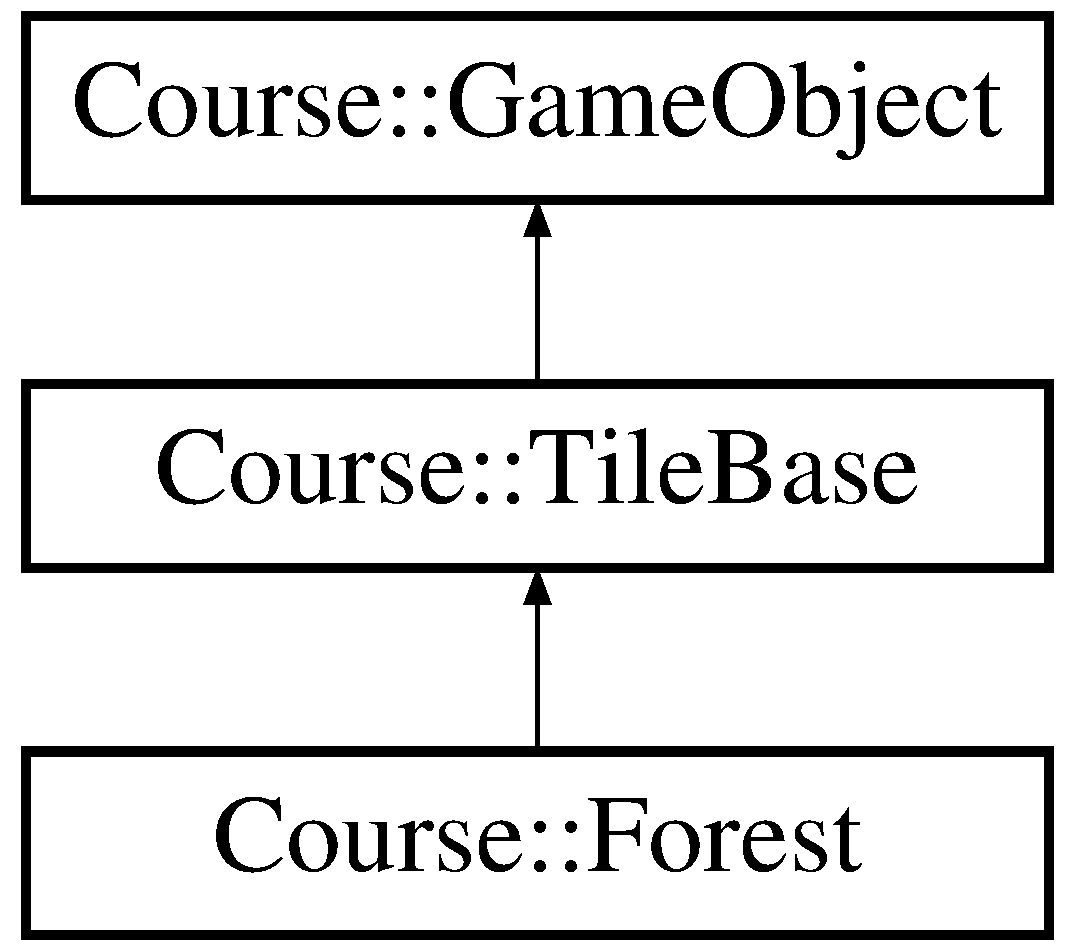
\includegraphics[height=3.000000cm]{classCourse_1_1Forest}
\end{center}
\end{figure}
\subsection*{Public Member Functions}
\begin{DoxyCompactItemize}
\item 
\hyperlink{classCourse_1_1Forest_a479a9c69f82dcd8cc2d0db81f067472b}{Forest} ()=delete
\begin{DoxyCompactList}\small\item\em Disabled parameterless constructor. \end{DoxyCompactList}\item 
\hyperlink{classCourse_1_1Forest_ab5e80525c9f03c02af4fd8e674d59485}{Forest} (const \hyperlink{classCourse_1_1Coordinate}{Coordinate} \&location, const std\-::shared\-\_\-ptr$<$ \hyperlink{classCourse_1_1iGameEventHandler}{i\-Game\-Event\-Handler} $>$ \&eventhandler, const std\-::shared\-\_\-ptr$<$ \hyperlink{classCourse_1_1iObjectManager}{i\-Object\-Manager} $>$ \&objectmanager, const unsigned int \&max\-\_\-build=2, const unsigned int \&max\-\_\-work=3, const \hyperlink{namespaceCourse_ab9a46ed9cd00485e318e5731ea2f78d9}{Resource\-Map} \&production=\hyperlink{namespaceCourse_1_1ConstResourceMaps_a7dcae89456b97bd487124b43c1b63a1c}{Const\-Resource\-Maps\-::\-F\-O\-R\-E\-S\-T\-\_\-\-B\-P})
\begin{DoxyCompactList}\small\item\em Constructor for the class. \end{DoxyCompactList}\item 
virtual \hyperlink{classCourse_1_1Forest_ac8e55f196786f07e92866e6ca1a6ae44}{$\sim$\-Forest} ()=default
\begin{DoxyCompactList}\small\item\em Default destructor. \end{DoxyCompactList}\item 
virtual std\-::string \hyperlink{classCourse_1_1Forest_a783378b8f5c1ec5d0c5c4a771291a902}{get\-Type} () const override
\begin{DoxyCompactList}\small\item\em get\-Type Returns a string describing objects type. This should be overriden in each inherited class. Makes checking object's type easier for students. \end{DoxyCompactList}\item 
void \hyperlink{classCourse_1_1Forest_a16ad633cd25afa705fbaefbc42efc2ae}{add\-Building} (const std\-::shared\-\_\-ptr$<$ \hyperlink{classCourse_1_1BuildingBase}{Building\-Base} $>$ \&building) override
\begin{DoxyCompactList}\small\item\em Adds a new building-\/object to the tile. Building in forest adds one hold-\/marker to the building. \end{DoxyCompactList}\end{DoxyCompactItemize}
\subsection*{Additional Inherited Members}


\subsection{Detailed Description}
The \hyperlink{classCourse_1_1Forest}{Forest} class represents \hyperlink{classCourse_1_1Forest}{Forest} in the gameworld. 

\hyperlink{classCourse_1_1Forest}{Forest} has Basic\-Production\-: \par

\begin{DoxyItemize}
\item Money = 1
\item Food = 3
\item Wood = 5
\item Stone = 1
\item Ore = 0
\end{DoxyItemize}

Building in the forest takes time. So buildings get extra hold-\/marker.

Tile supports 2 buildings. 

\subsection{Constructor \& Destructor Documentation}
\hypertarget{classCourse_1_1Forest_a479a9c69f82dcd8cc2d0db81f067472b}{\index{Course\-::\-Forest@{Course\-::\-Forest}!Forest@{Forest}}
\index{Forest@{Forest}!Course::Forest@{Course\-::\-Forest}}
\subsubsection[{Forest}]{\setlength{\rightskip}{0pt plus 5cm}Course\-::\-Forest\-::\-Forest (
\begin{DoxyParamCaption}
{}
\end{DoxyParamCaption}
)\hspace{0.3cm}{\ttfamily [delete]}}}\label{classCourse_1_1Forest_a479a9c69f82dcd8cc2d0db81f067472b}


Disabled parameterless constructor. 

\hypertarget{classCourse_1_1Forest_ab5e80525c9f03c02af4fd8e674d59485}{\index{Course\-::\-Forest@{Course\-::\-Forest}!Forest@{Forest}}
\index{Forest@{Forest}!Course::Forest@{Course\-::\-Forest}}
\subsubsection[{Forest}]{\setlength{\rightskip}{0pt plus 5cm}Course\-::\-Forest\-::\-Forest (
\begin{DoxyParamCaption}
\item[{const {\bf Coordinate} \&}]{location, }
\item[{const std\-::shared\-\_\-ptr$<$ {\bf i\-Game\-Event\-Handler} $>$ \&}]{eventhandler, }
\item[{const std\-::shared\-\_\-ptr$<$ {\bf i\-Object\-Manager} $>$ \&}]{objectmanager, }
\item[{const unsigned int \&}]{max\-\_\-build = {\ttfamily 2}, }
\item[{const unsigned int \&}]{max\-\_\-work = {\ttfamily 3}, }
\item[{const {\bf Resource\-Map} \&}]{production = {\ttfamily {\bf Const\-Resource\-Maps\-::\-F\-O\-R\-E\-S\-T\-\_\-\-B\-P}}}
\end{DoxyParamCaption}
)}}\label{classCourse_1_1Forest_ab5e80525c9f03c02af4fd8e674d59485}


Constructor for the class. 


\begin{DoxyParams}{Parameters}
{\em location} & is the \hyperlink{classCourse_1_1Coordinate}{Coordinate} where the Tile is located in the game. \\
\hline
{\em eventhandler} & points to the student's Game\-Event\-Handler. \\
\hline
\end{DoxyParams}
\hypertarget{classCourse_1_1Forest_ac8e55f196786f07e92866e6ca1a6ae44}{\index{Course\-::\-Forest@{Course\-::\-Forest}!$\sim$\-Forest@{$\sim$\-Forest}}
\index{$\sim$\-Forest@{$\sim$\-Forest}!Course::Forest@{Course\-::\-Forest}}
\subsubsection[{$\sim$\-Forest}]{\setlength{\rightskip}{0pt plus 5cm}virtual Course\-::\-Forest\-::$\sim$\-Forest (
\begin{DoxyParamCaption}
{}
\end{DoxyParamCaption}
)\hspace{0.3cm}{\ttfamily [virtual]}, {\ttfamily [default]}}}\label{classCourse_1_1Forest_ac8e55f196786f07e92866e6ca1a6ae44}


Default destructor. 



\subsection{Member Function Documentation}
\hypertarget{classCourse_1_1Forest_a16ad633cd25afa705fbaefbc42efc2ae}{\index{Course\-::\-Forest@{Course\-::\-Forest}!add\-Building@{add\-Building}}
\index{add\-Building@{add\-Building}!Course::Forest@{Course\-::\-Forest}}
\subsubsection[{add\-Building}]{\setlength{\rightskip}{0pt plus 5cm}void Course\-::\-Forest\-::add\-Building (
\begin{DoxyParamCaption}
\item[{const std\-::shared\-\_\-ptr$<$ {\bf Building\-Base} $>$ \&}]{building}
\end{DoxyParamCaption}
)\hspace{0.3cm}{\ttfamily [override]}, {\ttfamily [virtual]}}}\label{classCourse_1_1Forest_a16ad633cd25afa705fbaefbc42efc2ae}


Adds a new building-\/object to the tile. Building in forest adds one hold-\/marker to the building. 

Phases\-: \par

\begin{DoxyEnumerate}
\item Check that there is space for the building. \par

\item Call parent's add\-Building \par

\item Add a Hold\-Marker for the building. \par
 \begin{DoxyPostcond}{Postcondition}
Exception guarantee\-: Strong 
\end{DoxyPostcond}

\begin{DoxyExceptions}{Exceptions}
{\em \hyperlink{classCourse_1_1OwnerConflict}{Owner\-Conflict}} & -\/ If the tile's ownership prevents placing the {\bfseries building}. \\
\hline
{\em No\-Space} & -\/ If the tile doesn't have enough space for the {\bfseries building}. \\
\hline
\end{DoxyExceptions}

\end{DoxyEnumerate}

Reimplemented from \hyperlink{classCourse_1_1TileBase_add69a1e9ec009dedb28ce54c8535370b}{Course\-::\-Tile\-Base}.

\hypertarget{classCourse_1_1Forest_a783378b8f5c1ec5d0c5c4a771291a902}{\index{Course\-::\-Forest@{Course\-::\-Forest}!get\-Type@{get\-Type}}
\index{get\-Type@{get\-Type}!Course::Forest@{Course\-::\-Forest}}
\subsubsection[{get\-Type}]{\setlength{\rightskip}{0pt plus 5cm}std\-::string Course\-::\-Forest\-::get\-Type (
\begin{DoxyParamCaption}
{}
\end{DoxyParamCaption}
) const\hspace{0.3cm}{\ttfamily [override]}, {\ttfamily [virtual]}}}\label{classCourse_1_1Forest_a783378b8f5c1ec5d0c5c4a771291a902}


get\-Type Returns a string describing objects type. This should be overriden in each inherited class. Makes checking object's type easier for students. 

\begin{DoxyReturn}{Returns}
std\-::string that represents Object's type. 
\end{DoxyReturn}
\begin{DoxyPostcond}{Postcondition}
Exception guarantee\-: No-\/throw 
\end{DoxyPostcond}
\begin{DoxyNote}{Note}
You can use this in e.\-g. debugging and similar printing. 
\end{DoxyNote}


Reimplemented from \hyperlink{classCourse_1_1TileBase_af1a8aaa3407ad3ade7ffe8f2fb421288}{Course\-::\-Tile\-Base}.



The documentation for this class was generated from the following files\-:\begin{DoxyCompactItemize}
\item 
Course/\-Course\-Lib/tiles/\hyperlink{forest_8h}{forest.\-h}\item 
Course/\-Course\-Lib/tiles/\hyperlink{forest_8cpp}{forest.\-cpp}\end{DoxyCompactItemize}

\hypertarget{classGame_1_1GameEventHandler}{\section{Game\-:\-:Game\-Event\-Handler Class Reference}
\label{classGame_1_1GameEventHandler}\index{Game\-::\-Game\-Event\-Handler@{Game\-::\-Game\-Event\-Handler}}
}


The \hyperlink{classGame_1_1GameEventHandler}{Game\-Event\-Handler} class controls and stores the game's status.  




{\ttfamily \#include $<$gameeventhandler.\-h$>$}

Inheritance diagram for Game\-:\-:Game\-Event\-Handler\-:\begin{figure}[H]
\begin{center}
\leavevmode
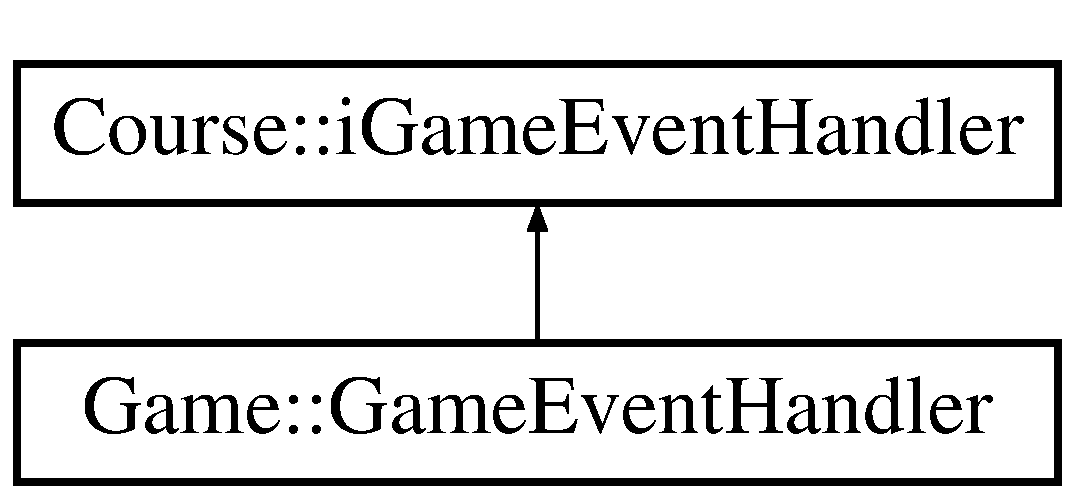
\includegraphics[height=2.000000cm]{classGame_1_1GameEventHandler}
\end{center}
\end{figure}
\subsection*{Public Member Functions}
\begin{DoxyCompactItemize}
\item 
\hyperlink{classGame_1_1GameEventHandler_a5d2bcae44b3675121b2714f5c09f6469}{Game\-Event\-Handler} ()
\begin{DoxyCompactList}\small\item\em Constructor for the class. \end{DoxyCompactList}\item 
bool \hyperlink{classGame_1_1GameEventHandler_a94426aa16bad3385bc3d75249596325c}{modify\-Resource} (std\-::shared\-\_\-ptr$<$ \hyperlink{classCourse_1_1PlayerBase}{Course\-::\-Player\-Base} $>$ player, \hyperlink{namespaceCourse_a02d49c04029594d4adba79b84bb85f65}{Course\-::\-Basic\-Resource} resource, int amount)
\begin{DoxyCompactList}\small\item\em Modify \hyperlink{classGame_1_1Player}{Player}'s resource. Can be used to both sum or subtract. \end{DoxyCompactList}\item 
bool \hyperlink{classGame_1_1GameEventHandler_af2f37590702d555bb6635a6a7793ebb2}{modify\-Resources} (std\-::shared\-\_\-ptr$<$ \hyperlink{classCourse_1_1PlayerBase}{Course\-::\-Player\-Base} $>$ player, \hyperlink{namespaceCourse_ab9a46ed9cd00485e318e5731ea2f78d9}{Course\-::\-Resource\-Map} resources)
\begin{DoxyCompactList}\small\item\em Modify \hyperlink{classGame_1_1Player}{Player}'s resources. Can be used to both sum or subtract. \end{DoxyCompactList}\item 
std\-::shared\-\_\-ptr$<$ \hyperlink{classGame_1_1Player}{Player} $>$ \hyperlink{classGame_1_1GameEventHandler_a6db7a31e0c0484848d74703aec79189b}{get\-Player\-In\-Turn} ()
\begin{DoxyCompactList}\small\item\em Gets the player in turn. \end{DoxyCompactList}\item 
void \hyperlink{classGame_1_1GameEventHandler_aa05246452c9b7304c418c502db72545d}{set\-Player\-In\-Turn} (const std\-::shared\-\_\-ptr$<$ \hyperlink{classGame_1_1Player}{Player} $>$ player)
\begin{DoxyCompactList}\small\item\em Sets the player in turn. \end{DoxyCompactList}\item 
std\-::vector$<$ std\-::shared\-\_\-ptr\\*
$<$ \hyperlink{classGame_1_1Player}{Player} $>$ $>$ \hyperlink{classGame_1_1GameEventHandler_a3e8a68eec25834d491e81c68a0a1a318}{check\-Win\-Condition} (std\-::vector$<$ std\-::shared\-\_\-ptr$<$ \hyperlink{classGame_1_1Player}{Player} $>$$>$ players)
\begin{DoxyCompactList}\small\item\em Checks if players have won. \end{DoxyCompactList}\item 
void \hyperlink{classGame_1_1GameEventHandler_a3ef61837daa4a8cba540986bdfdfb3a6}{set\-Resources\-To\-Win} (const int resources\-To\-Win)
\begin{DoxyCompactList}\small\item\em Sets the sum of resources needed to win the game. \end{DoxyCompactList}\item 
void \hyperlink{classGame_1_1GameEventHandler_a7e923c78df72600509dee5e292052653}{set\-Buying\-Flag} (const bool buying)
\begin{DoxyCompactList}\small\item\em Sets the flag telling that we are in the middle of buying something. \end{DoxyCompactList}\item 
bool \hyperlink{classGame_1_1GameEventHandler_a76fe6c9beff8949f31dea0f0111a508a}{is\-Player\-Buying} () const 
\begin{DoxyCompactList}\small\item\em Checks if we are in the middle of buying something. \end{DoxyCompactList}\item 
int \hyperlink{classGame_1_1GameEventHandler_ad4c9a8438df151e4c191c31b4bfdcec1}{get\-Rounds} () const 
\begin{DoxyCompactList}\small\item\em Gets the amount of rounds the game has been played. \end{DoxyCompactList}\item 
int \hyperlink{classGame_1_1GameEventHandler_a9a6af0f0397815127f8a9d07f0c1c9dc}{increase\-Rounds} ()
\begin{DoxyCompactList}\small\item\em Increases the game round by one. \end{DoxyCompactList}\end{DoxyCompactItemize}
\subsection*{Private Member Functions}
\begin{DoxyCompactItemize}
\item 
bool \hyperlink{classGame_1_1GameEventHandler_a8340221ba757fe26a656ded19f60a540}{player\-Has\-Won} (std\-::shared\-\_\-ptr$<$ \hyperlink{classGame_1_1Player}{Player} $>$ player)
\begin{DoxyCompactList}\small\item\em Checks if a player has won. \end{DoxyCompactList}\end{DoxyCompactItemize}
\subsection*{Private Attributes}
\begin{DoxyCompactItemize}
\item 
int \hyperlink{classGame_1_1GameEventHandler_aea76258b522fd99ee263be7d9893d119}{m\-\_\-rounds} = 1
\item 
int \hyperlink{classGame_1_1GameEventHandler_aae97f288e69193c5adfd42412dab61a3}{m\-\_\-resources\-To\-Win}
\item 
std\-::weak\-\_\-ptr$<$ \hyperlink{classGame_1_1Player}{Player} $>$ \hyperlink{classGame_1_1GameEventHandler_ad28b5869e241612eeb2b914cde6cb5ed}{m\-\_\-player\-In\-Turn}
\item 
bool \hyperlink{classGame_1_1GameEventHandler_a786fce818b23233b7d7213f43daf03b0}{m\-\_\-player\-Buying} = false
\end{DoxyCompactItemize}


\subsection{Detailed Description}
The \hyperlink{classGame_1_1GameEventHandler}{Game\-Event\-Handler} class controls and stores the game's status. 

Only one of these should exists at any given point in the time 

\subsection{Constructor \& Destructor Documentation}
\hypertarget{classGame_1_1GameEventHandler_a5d2bcae44b3675121b2714f5c09f6469}{\index{Game\-::\-Game\-Event\-Handler@{Game\-::\-Game\-Event\-Handler}!Game\-Event\-Handler@{Game\-Event\-Handler}}
\index{Game\-Event\-Handler@{Game\-Event\-Handler}!Game::GameEventHandler@{Game\-::\-Game\-Event\-Handler}}
\subsubsection[{Game\-Event\-Handler}]{\setlength{\rightskip}{0pt plus 5cm}Game\-::\-Game\-Event\-Handler\-::\-Game\-Event\-Handler (
\begin{DoxyParamCaption}
{}
\end{DoxyParamCaption}
)}}\label{classGame_1_1GameEventHandler_a5d2bcae44b3675121b2714f5c09f6469}


Constructor for the class. 



\subsection{Member Function Documentation}
\hypertarget{classGame_1_1GameEventHandler_a3e8a68eec25834d491e81c68a0a1a318}{\index{Game\-::\-Game\-Event\-Handler@{Game\-::\-Game\-Event\-Handler}!check\-Win\-Condition@{check\-Win\-Condition}}
\index{check\-Win\-Condition@{check\-Win\-Condition}!Game::GameEventHandler@{Game\-::\-Game\-Event\-Handler}}
\subsubsection[{check\-Win\-Condition}]{\setlength{\rightskip}{0pt plus 5cm}std\-::vector$<$ std\-::shared\-\_\-ptr$<$ {\bf Player} $>$ $>$ Game\-::\-Game\-Event\-Handler\-::check\-Win\-Condition (
\begin{DoxyParamCaption}
\item[{std\-::vector$<$ std\-::shared\-\_\-ptr$<$ {\bf Player} $>$$>$}]{players}
\end{DoxyParamCaption}
)}}\label{classGame_1_1GameEventHandler_a3e8a68eec25834d491e81c68a0a1a318}


Checks if players have won. 


\begin{DoxyParams}{Parameters}
{\em players} & Vector of pointers to \hyperlink{classGame_1_1Player}{Player} objects. \\
\hline
\end{DoxyParams}
\begin{DoxyReturn}{Returns}
Vector of pointers to \hyperlink{classGame_1_1Player}{Player} objects that have won 
\end{DoxyReturn}
\hypertarget{classGame_1_1GameEventHandler_a6db7a31e0c0484848d74703aec79189b}{\index{Game\-::\-Game\-Event\-Handler@{Game\-::\-Game\-Event\-Handler}!get\-Player\-In\-Turn@{get\-Player\-In\-Turn}}
\index{get\-Player\-In\-Turn@{get\-Player\-In\-Turn}!Game::GameEventHandler@{Game\-::\-Game\-Event\-Handler}}
\subsubsection[{get\-Player\-In\-Turn}]{\setlength{\rightskip}{0pt plus 5cm}std\-::shared\-\_\-ptr$<$ {\bf Player} $>$ Game\-::\-Game\-Event\-Handler\-::get\-Player\-In\-Turn (
\begin{DoxyParamCaption}
{}
\end{DoxyParamCaption}
)}}\label{classGame_1_1GameEventHandler_a6db7a31e0c0484848d74703aec79189b}


Gets the player in turn. 

\begin{DoxyReturn}{Returns}
the player whose turn it is currently 
\end{DoxyReturn}
\hypertarget{classGame_1_1GameEventHandler_ad4c9a8438df151e4c191c31b4bfdcec1}{\index{Game\-::\-Game\-Event\-Handler@{Game\-::\-Game\-Event\-Handler}!get\-Rounds@{get\-Rounds}}
\index{get\-Rounds@{get\-Rounds}!Game::GameEventHandler@{Game\-::\-Game\-Event\-Handler}}
\subsubsection[{get\-Rounds}]{\setlength{\rightskip}{0pt plus 5cm}int Game\-::\-Game\-Event\-Handler\-::get\-Rounds (
\begin{DoxyParamCaption}
{}
\end{DoxyParamCaption}
) const}}\label{classGame_1_1GameEventHandler_ad4c9a8438df151e4c191c31b4bfdcec1}


Gets the amount of rounds the game has been played. 

\begin{DoxyReturn}{Returns}
Amount of rounds 
\end{DoxyReturn}
\hypertarget{classGame_1_1GameEventHandler_a9a6af0f0397815127f8a9d07f0c1c9dc}{\index{Game\-::\-Game\-Event\-Handler@{Game\-::\-Game\-Event\-Handler}!increase\-Rounds@{increase\-Rounds}}
\index{increase\-Rounds@{increase\-Rounds}!Game::GameEventHandler@{Game\-::\-Game\-Event\-Handler}}
\subsubsection[{increase\-Rounds}]{\setlength{\rightskip}{0pt plus 5cm}int Game\-::\-Game\-Event\-Handler\-::increase\-Rounds (
\begin{DoxyParamCaption}
{}
\end{DoxyParamCaption}
)}}\label{classGame_1_1GameEventHandler_a9a6af0f0397815127f8a9d07f0c1c9dc}


Increases the game round by one. 

\begin{DoxyReturn}{Returns}
Amount of rounds after the increase 
\end{DoxyReturn}
\hypertarget{classGame_1_1GameEventHandler_a76fe6c9beff8949f31dea0f0111a508a}{\index{Game\-::\-Game\-Event\-Handler@{Game\-::\-Game\-Event\-Handler}!is\-Player\-Buying@{is\-Player\-Buying}}
\index{is\-Player\-Buying@{is\-Player\-Buying}!Game::GameEventHandler@{Game\-::\-Game\-Event\-Handler}}
\subsubsection[{is\-Player\-Buying}]{\setlength{\rightskip}{0pt plus 5cm}bool Game\-::\-Game\-Event\-Handler\-::is\-Player\-Buying (
\begin{DoxyParamCaption}
{}
\end{DoxyParamCaption}
) const}}\label{classGame_1_1GameEventHandler_a76fe6c9beff8949f31dea0f0111a508a}


Checks if we are in the middle of buying something. 

\begin{DoxyReturn}{Returns}
Boolean value telling if we are buying something 
\end{DoxyReturn}
\hypertarget{classGame_1_1GameEventHandler_a94426aa16bad3385bc3d75249596325c}{\index{Game\-::\-Game\-Event\-Handler@{Game\-::\-Game\-Event\-Handler}!modify\-Resource@{modify\-Resource}}
\index{modify\-Resource@{modify\-Resource}!Game::GameEventHandler@{Game\-::\-Game\-Event\-Handler}}
\subsubsection[{modify\-Resource}]{\setlength{\rightskip}{0pt plus 5cm}bool Game\-::\-Game\-Event\-Handler\-::modify\-Resource (
\begin{DoxyParamCaption}
\item[{std\-::shared\-\_\-ptr$<$ {\bf Course\-::\-Player\-Base} $>$}]{player, }
\item[{{\bf Course\-::\-Basic\-Resource}}]{resource, }
\item[{int}]{amount}
\end{DoxyParamCaption}
)\hspace{0.3cm}{\ttfamily [virtual]}}}\label{classGame_1_1GameEventHandler_a94426aa16bad3385bc3d75249596325c}


Modify \hyperlink{classGame_1_1Player}{Player}'s resource. Can be used to both sum or subtract. 


\begin{DoxyParams}{Parameters}
{\em player} & Pointer to the \hyperlink{classGame_1_1Player}{Player} whose resource is being modified. \\
\hline
{\em resource} & Defines the modified resource. \\
\hline
{\em amount} & Defines the amount of change. \\
\hline
\end{DoxyParams}
\begin{DoxyPostcond}{Postcondition}
Exception guarantee\-: Basic 
\end{DoxyPostcond}
\begin{DoxyReturn}{Returns}
True -\/ Modification was succesful. \par
False -\/ Modification failed. \par

\end{DoxyReturn}


Implements \hyperlink{classCourse_1_1iGameEventHandler_abcf1e403dc6081dc348e892fcd197e83}{Course\-::i\-Game\-Event\-Handler}.

\hypertarget{classGame_1_1GameEventHandler_af2f37590702d555bb6635a6a7793ebb2}{\index{Game\-::\-Game\-Event\-Handler@{Game\-::\-Game\-Event\-Handler}!modify\-Resources@{modify\-Resources}}
\index{modify\-Resources@{modify\-Resources}!Game::GameEventHandler@{Game\-::\-Game\-Event\-Handler}}
\subsubsection[{modify\-Resources}]{\setlength{\rightskip}{0pt plus 5cm}bool Game\-::\-Game\-Event\-Handler\-::modify\-Resources (
\begin{DoxyParamCaption}
\item[{std\-::shared\-\_\-ptr$<$ {\bf Course\-::\-Player\-Base} $>$}]{player, }
\item[{{\bf Course\-::\-Resource\-Map}}]{resources}
\end{DoxyParamCaption}
)\hspace{0.3cm}{\ttfamily [virtual]}}}\label{classGame_1_1GameEventHandler_af2f37590702d555bb6635a6a7793ebb2}


Modify \hyperlink{classGame_1_1Player}{Player}'s resources. Can be used to both sum or subtract. 


\begin{DoxyParams}{Parameters}
{\em player} & Pointer to the \hyperlink{classGame_1_1Player}{Player} whose resources are being modified. \\
\hline
{\em resources} & Resource\-Map containing change amounts. \\
\hline
\end{DoxyParams}
\begin{DoxyReturn}{Returns}
True -\/ Modification was succesful. \par
False -\/ Modification failed. \par

\end{DoxyReturn}


Implements \hyperlink{classCourse_1_1iGameEventHandler_aafe82af26594e1261af045b2a896cd4e}{Course\-::i\-Game\-Event\-Handler}.

\hypertarget{classGame_1_1GameEventHandler_a8340221ba757fe26a656ded19f60a540}{\index{Game\-::\-Game\-Event\-Handler@{Game\-::\-Game\-Event\-Handler}!player\-Has\-Won@{player\-Has\-Won}}
\index{player\-Has\-Won@{player\-Has\-Won}!Game::GameEventHandler@{Game\-::\-Game\-Event\-Handler}}
\subsubsection[{player\-Has\-Won}]{\setlength{\rightskip}{0pt plus 5cm}bool Game\-::\-Game\-Event\-Handler\-::player\-Has\-Won (
\begin{DoxyParamCaption}
\item[{std\-::shared\-\_\-ptr$<$ {\bf Player} $>$}]{player}
\end{DoxyParamCaption}
)\hspace{0.3cm}{\ttfamily [private]}}}\label{classGame_1_1GameEventHandler_a8340221ba757fe26a656ded19f60a540}


Checks if a player has won. 


\begin{DoxyParams}{Parameters}
{\em player} & Pointer to the \hyperlink{classGame_1_1Player}{Player}. \\
\hline
\end{DoxyParams}
\begin{DoxyReturn}{Returns}
True -\/ \hyperlink{classGame_1_1Player}{Player} has won. \par
False -\/ \hyperlink{classGame_1_1Player}{Player} hasn't won. \par

\end{DoxyReturn}
\hypertarget{classGame_1_1GameEventHandler_a7e923c78df72600509dee5e292052653}{\index{Game\-::\-Game\-Event\-Handler@{Game\-::\-Game\-Event\-Handler}!set\-Buying\-Flag@{set\-Buying\-Flag}}
\index{set\-Buying\-Flag@{set\-Buying\-Flag}!Game::GameEventHandler@{Game\-::\-Game\-Event\-Handler}}
\subsubsection[{set\-Buying\-Flag}]{\setlength{\rightskip}{0pt plus 5cm}void Game\-::\-Game\-Event\-Handler\-::set\-Buying\-Flag (
\begin{DoxyParamCaption}
\item[{const bool}]{buying}
\end{DoxyParamCaption}
)}}\label{classGame_1_1GameEventHandler_a7e923c78df72600509dee5e292052653}


Sets the flag telling that we are in the middle of buying something. 


\begin{DoxyParams}{Parameters}
{\em buying} & Flag for buying \\
\hline
\end{DoxyParams}
\hypertarget{classGame_1_1GameEventHandler_aa05246452c9b7304c418c502db72545d}{\index{Game\-::\-Game\-Event\-Handler@{Game\-::\-Game\-Event\-Handler}!set\-Player\-In\-Turn@{set\-Player\-In\-Turn}}
\index{set\-Player\-In\-Turn@{set\-Player\-In\-Turn}!Game::GameEventHandler@{Game\-::\-Game\-Event\-Handler}}
\subsubsection[{set\-Player\-In\-Turn}]{\setlength{\rightskip}{0pt plus 5cm}void Game\-::\-Game\-Event\-Handler\-::set\-Player\-In\-Turn (
\begin{DoxyParamCaption}
\item[{const std\-::shared\-\_\-ptr$<$ {\bf Player} $>$}]{player}
\end{DoxyParamCaption}
)}}\label{classGame_1_1GameEventHandler_aa05246452c9b7304c418c502db72545d}


Sets the player in turn. 


\begin{DoxyParams}{Parameters}
{\em player} & Pointer to the \hyperlink{classGame_1_1Player}{Player}. \\
\hline
\end{DoxyParams}
\hypertarget{classGame_1_1GameEventHandler_a3ef61837daa4a8cba540986bdfdfb3a6}{\index{Game\-::\-Game\-Event\-Handler@{Game\-::\-Game\-Event\-Handler}!set\-Resources\-To\-Win@{set\-Resources\-To\-Win}}
\index{set\-Resources\-To\-Win@{set\-Resources\-To\-Win}!Game::GameEventHandler@{Game\-::\-Game\-Event\-Handler}}
\subsubsection[{set\-Resources\-To\-Win}]{\setlength{\rightskip}{0pt plus 5cm}void Game\-::\-Game\-Event\-Handler\-::set\-Resources\-To\-Win (
\begin{DoxyParamCaption}
\item[{const int}]{resources\-To\-Win}
\end{DoxyParamCaption}
)}}\label{classGame_1_1GameEventHandler_a3ef61837daa4a8cba540986bdfdfb3a6}


Sets the sum of resources needed to win the game. 


\begin{DoxyParams}{Parameters}
{\em resources\-To\-Win} & Amount of resources as a sum \\
\hline
\end{DoxyParams}


\subsection{Member Data Documentation}
\hypertarget{classGame_1_1GameEventHandler_a786fce818b23233b7d7213f43daf03b0}{\index{Game\-::\-Game\-Event\-Handler@{Game\-::\-Game\-Event\-Handler}!m\-\_\-player\-Buying@{m\-\_\-player\-Buying}}
\index{m\-\_\-player\-Buying@{m\-\_\-player\-Buying}!Game::GameEventHandler@{Game\-::\-Game\-Event\-Handler}}
\subsubsection[{m\-\_\-player\-Buying}]{\setlength{\rightskip}{0pt plus 5cm}bool Game\-::\-Game\-Event\-Handler\-::m\-\_\-player\-Buying = false\hspace{0.3cm}{\ttfamily [private]}}}\label{classGame_1_1GameEventHandler_a786fce818b23233b7d7213f43daf03b0}
\hypertarget{classGame_1_1GameEventHandler_ad28b5869e241612eeb2b914cde6cb5ed}{\index{Game\-::\-Game\-Event\-Handler@{Game\-::\-Game\-Event\-Handler}!m\-\_\-player\-In\-Turn@{m\-\_\-player\-In\-Turn}}
\index{m\-\_\-player\-In\-Turn@{m\-\_\-player\-In\-Turn}!Game::GameEventHandler@{Game\-::\-Game\-Event\-Handler}}
\subsubsection[{m\-\_\-player\-In\-Turn}]{\setlength{\rightskip}{0pt plus 5cm}std\-::weak\-\_\-ptr$<${\bf Player}$>$ Game\-::\-Game\-Event\-Handler\-::m\-\_\-player\-In\-Turn\hspace{0.3cm}{\ttfamily [private]}}}\label{classGame_1_1GameEventHandler_ad28b5869e241612eeb2b914cde6cb5ed}
\hypertarget{classGame_1_1GameEventHandler_aae97f288e69193c5adfd42412dab61a3}{\index{Game\-::\-Game\-Event\-Handler@{Game\-::\-Game\-Event\-Handler}!m\-\_\-resources\-To\-Win@{m\-\_\-resources\-To\-Win}}
\index{m\-\_\-resources\-To\-Win@{m\-\_\-resources\-To\-Win}!Game::GameEventHandler@{Game\-::\-Game\-Event\-Handler}}
\subsubsection[{m\-\_\-resources\-To\-Win}]{\setlength{\rightskip}{0pt plus 5cm}int Game\-::\-Game\-Event\-Handler\-::m\-\_\-resources\-To\-Win\hspace{0.3cm}{\ttfamily [private]}}}\label{classGame_1_1GameEventHandler_aae97f288e69193c5adfd42412dab61a3}
\hypertarget{classGame_1_1GameEventHandler_aea76258b522fd99ee263be7d9893d119}{\index{Game\-::\-Game\-Event\-Handler@{Game\-::\-Game\-Event\-Handler}!m\-\_\-rounds@{m\-\_\-rounds}}
\index{m\-\_\-rounds@{m\-\_\-rounds}!Game::GameEventHandler@{Game\-::\-Game\-Event\-Handler}}
\subsubsection[{m\-\_\-rounds}]{\setlength{\rightskip}{0pt plus 5cm}int Game\-::\-Game\-Event\-Handler\-::m\-\_\-rounds = 1\hspace{0.3cm}{\ttfamily [private]}}}\label{classGame_1_1GameEventHandler_aea76258b522fd99ee263be7d9893d119}


The documentation for this class was generated from the following files\-:\begin{DoxyCompactItemize}
\item 
Game/core/\hyperlink{gameeventhandler_8h}{gameeventhandler.\-h}\item 
Game/core/\hyperlink{gameeventhandler_8cpp}{gameeventhandler.\-cpp}\end{DoxyCompactItemize}

\hypertarget{classCourse_1_1GameObject}{\section{Course\-:\-:Game\-Object Class Reference}
\label{classCourse_1_1GameObject}\index{Course\-::\-Game\-Object@{Course\-::\-Game\-Object}}
}


The \hyperlink{classCourse_1_1GameObject}{Game\-Object} class is base-\/class that contain's general information on different Objects in game.  




{\ttfamily \#include $<$gameobject.\-h$>$}

Inheritance diagram for Course\-:\-:Game\-Object\-:\begin{figure}[H]
\begin{center}
\leavevmode
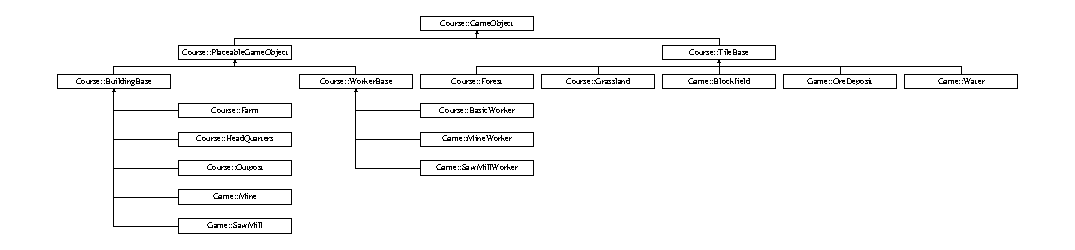
\includegraphics[height=2.916667cm]{classCourse_1_1GameObject}
\end{center}
\end{figure}
\subsection*{Public Member Functions}
\begin{DoxyCompactItemize}
\item 
\hyperlink{classCourse_1_1GameObject_ad250968a18df7c5de3ac55a72a3a0326}{Game\-Object} (const \hyperlink{classCourse_1_1GameObject}{Game\-Object} \&original)
\begin{DoxyCompactList}\small\item\em A simple copy-\/constructor for \hyperlink{classCourse_1_1GameObject}{Game\-Object}. \end{DoxyCompactList}\item 
\hyperlink{classCourse_1_1GameObject_a4eeabd6bdee20a60dc091fde67340cde}{Game\-Object} (const std\-::shared\-\_\-ptr$<$ \hyperlink{classCourse_1_1iGameEventHandler}{i\-Game\-Event\-Handler} $>$ \&eventhandler=\{nullptr\}, const std\-::shared\-\_\-ptr$<$ \hyperlink{classCourse_1_1iObjectManager}{i\-Object\-Manager} $>$ \&objectmanager=\{nullptr\})
\begin{DoxyCompactList}\small\item\em Constructor that only specifies Game\-Event\-Handler and Object\-Manager. \end{DoxyCompactList}\item 
\hyperlink{classCourse_1_1GameObject_a3daab55fb0f661324883acceaee817d0}{Game\-Object} (const std\-::shared\-\_\-ptr$<$ \hyperlink{classCourse_1_1PlayerBase}{Player\-Base} $>$ \&owner, const std\-::shared\-\_\-ptr$<$ \hyperlink{classCourse_1_1iGameEventHandler}{i\-Game\-Event\-Handler} $>$ \&eventhandler=\{nullptr\}, const std\-::shared\-\_\-ptr$<$ \hyperlink{classCourse_1_1iObjectManager}{i\-Object\-Manager} $>$ \&objectmanager=\{nullptr\})
\begin{DoxyCompactList}\small\item\em \hyperlink{classCourse_1_1GameObject}{Game\-Object} constructor that can specify an owner. \end{DoxyCompactList}\item 
\hyperlink{classCourse_1_1GameObject_a2b5425b9b112077d35b576031dc8bf74}{Game\-Object} (const \hyperlink{classCourse_1_1Coordinate}{Coordinate} \&coordinate, const std\-::shared\-\_\-ptr$<$ \hyperlink{classCourse_1_1PlayerBase}{Player\-Base} $>$ \&owner, const std\-::shared\-\_\-ptr$<$ \hyperlink{classCourse_1_1iGameEventHandler}{i\-Game\-Event\-Handler} $>$ \&eventhandler=\{nullptr\}, const std\-::shared\-\_\-ptr$<$ \hyperlink{classCourse_1_1iObjectManager}{i\-Object\-Manager} $>$ \&objectmanager=\{nullptr\})
\begin{DoxyCompactList}\small\item\em \hyperlink{classCourse_1_1GameObject}{Game\-Object} constructor that can specify a coordinate and an owner. \end{DoxyCompactList}\item 
\hyperlink{classCourse_1_1GameObject_a6dda384344838b53a330629c15b060c2}{Game\-Object} (const \hyperlink{classCourse_1_1Coordinate}{Coordinate} \&coordinate, const std\-::shared\-\_\-ptr$<$ \hyperlink{classCourse_1_1iGameEventHandler}{i\-Game\-Event\-Handler} $>$ \&eventhandler=\{nullptr\}, const std\-::shared\-\_\-ptr$<$ \hyperlink{classCourse_1_1iObjectManager}{i\-Object\-Manager} $>$ \&objectmanager=\{nullptr\})
\begin{DoxyCompactList}\small\item\em \hyperlink{classCourse_1_1GameObject}{Game\-Object} constructor that can specify a coordinate. \end{DoxyCompactList}\item 
virtual \hyperlink{classCourse_1_1GameObject_abfa4185247b43636bf53897a4731a763}{$\sim$\-Game\-Object} ()=default
\begin{DoxyCompactList}\small\item\em $\sim$\-Game\-Object Default destructor. \end{DoxyCompactList}\item 
virtual void \hyperlink{classCourse_1_1GameObject_a81a67b658271a5f3e08f5583e7075b27}{set\-Owner} (const std\-::shared\-\_\-ptr$<$ \hyperlink{classCourse_1_1PlayerBase}{Player\-Base} $>$ \&owner) final
\begin{DoxyCompactList}\small\item\em Change \hyperlink{classCourse_1_1GameObject}{Game\-Object}'s \char`\"{}owner\char`\"{}. \end{DoxyCompactList}\item 
virtual void \hyperlink{classCourse_1_1GameObject_acdb9942a83ae7247b6b5f241e4c6da3a}{set\-Coordinate} (const std\-::shared\-\_\-ptr$<$ \hyperlink{classCourse_1_1Coordinate}{Coordinate} $>$ \&coordinate) final
\begin{DoxyCompactList}\small\item\em Change \hyperlink{classCourse_1_1GameObject}{Game\-Object}'s coordinate with a shared pointer to a coordinate. \end{DoxyCompactList}\item 
virtual void \hyperlink{classCourse_1_1GameObject_a5161d3771985aa0bc64f238c29887c34}{set\-Coordinate} (const \hyperlink{classCourse_1_1Coordinate}{Coordinate} \&coordinate) final
\begin{DoxyCompactList}\small\item\em Change \hyperlink{classCourse_1_1GameObject}{Game\-Object}'s coordinate. \end{DoxyCompactList}\item 
virtual void \hyperlink{classCourse_1_1GameObject_a9deee37f01710a4d5b8968caadc01b0e}{unset\-Coordinate} () final
\begin{DoxyCompactList}\small\item\em Removes the coordinate from \hyperlink{classCourse_1_1GameObject}{Game\-Object}. \end{DoxyCompactList}\item 
virtual void \hyperlink{classCourse_1_1GameObject_a7b0790f1bd831bd7efa68b7d135a32cb}{set\-Descriptions} (const \hyperlink{namespaceCourse_aed04c39dde5a591d4b353686d3d0e306}{Description\-Map} \&descriptions) final
\begin{DoxyCompactList}\small\item\em Change \hyperlink{classCourse_1_1GameObject}{Game\-Object}'s \char`\"{}descriptions\char`\"{}-\/map. \end{DoxyCompactList}\item 
virtual void \hyperlink{classCourse_1_1GameObject_a0af72e3a237cefda5dc6d2b13a6e5881}{add\-Description} (const std\-::string \&key, const std\-::string \&content) final
\begin{DoxyCompactList}\small\item\em Adds a new description to description map. \end{DoxyCompactList}\item 
virtual void \hyperlink{classCourse_1_1GameObject_af94a781ae557e795e4fca8932cb05abb}{set\-Description} (const std\-::string \&key, const std\-::string \&content) final
\begin{DoxyCompactList}\small\item\em Sets a description for the specified key. \end{DoxyCompactList}\item 
virtual std\-::string \hyperlink{classCourse_1_1GameObject_a9b9e4340460debcbc7f97e48ef6fb437}{get\-Description} (const std\-::string \&key) const final
\begin{DoxyCompactList}\small\item\em Returns the content with specified key from the descriptions. \end{DoxyCompactList}\item 
virtual void \hyperlink{classCourse_1_1GameObject_a94262eeb0c85d5285e275080d19eb334}{remove\-Description} (const std\-::string \&key) final
\begin{DoxyCompactList}\small\item\em Removes the content with specified key from the descriptions. \end{DoxyCompactList}\item 
virtual void \hyperlink{classCourse_1_1GameObject_adbd24d1cdfbf317bd85ca27732be6a8a}{remove\-Descriptions} () final
\begin{DoxyCompactList}\small\item\em Removes all content from descriptions. \end{DoxyCompactList}\item 
virtual std\-::shared\-\_\-ptr\\*
$<$ \hyperlink{classCourse_1_1PlayerBase}{Player\-Base} $>$ \hyperlink{classCourse_1_1GameObject_a3c923e5d874cada8661d37002073c111}{get\-Owner} () const final
\begin{DoxyCompactList}\small\item\em Returns \hyperlink{classCourse_1_1GameObject}{Game\-Object}'s owner. \end{DoxyCompactList}\item 
virtual std\-::shared\-\_\-ptr\\*
$<$ \hyperlink{classCourse_1_1Coordinate}{Coordinate} $>$ \hyperlink{classCourse_1_1GameObject_a51383b004b38598b7287ed832d43150a}{get\-Coordinate\-Ptr} () const final
\begin{DoxyCompactList}\small\item\em Returns a pointer to a copy of \hyperlink{classCourse_1_1GameObject}{Game\-Object}'s coordinate. \end{DoxyCompactList}\item 
virtual \hyperlink{classCourse_1_1Coordinate}{Coordinate} \hyperlink{classCourse_1_1GameObject_ae3f1f045d5731fa85c9638a1bfa191fe}{get\-Coordinate} () const final
\begin{DoxyCompactList}\small\item\em Returns \hyperlink{classCourse_1_1GameObject}{Game\-Object}'s current coordinate. \end{DoxyCompactList}\item 
virtual std\-::map$<$ std\-::string, \\*
std\-::string $>$ \hyperlink{classCourse_1_1GameObject_aefe5a503378bfc7f6559a8e822491837}{get\-Descriptions} () const final
\begin{DoxyCompactList}\small\item\em Returns the map of descriptions in \hyperlink{classCourse_1_1GameObject}{Game\-Object}. \end{DoxyCompactList}\item 
virtual std\-::string \hyperlink{classCourse_1_1GameObject_aeecb0b8f5ed8d7b379e0e38ef4ebba10}{get\-Type} () const 
\begin{DoxyCompactList}\small\item\em get\-Type Returns a string describing objects type. This should be overriden in each inherited class. Makes checking object's type easier for students. \end{DoxyCompactList}\item 
virtual bool \hyperlink{classCourse_1_1GameObject_a1c592d7013f54f62be5eb6a99fcdfd64}{has\-Same\-Owner\-As} (const std\-::shared\-\_\-ptr$<$ \hyperlink{classCourse_1_1GameObject}{Game\-Object} $>$ \&other) const final
\begin{DoxyCompactList}\small\item\em Function to compare if objects have same owner. \end{DoxyCompactList}\item 
virtual bool \hyperlink{classCourse_1_1GameObject_a8d6a0a93150e7e4ca90176c028a037e1}{has\-Same\-Coordinate\-As} (const std\-::shared\-\_\-ptr$<$ \hyperlink{classCourse_1_1GameObject}{Game\-Object} $>$ \&other) const final
\begin{DoxyCompactList}\small\item\em has\-\_\-same\-\_\-coordinate \end{DoxyCompactList}\end{DoxyCompactItemize}
\subsection*{Public Attributes}
\begin{DoxyCompactItemize}
\item 
const \hyperlink{namespaceCourse_a9a16e743c9813da00109e4991afd2f3e}{Object\-Id} \hyperlink{classCourse_1_1GameObject_a6524f318100ebbaa1571996a2cab18a8}{I\-D}
\begin{DoxyCompactList}\small\item\em I\-D is a constant value that can be used to identify Game\-Objects through I\-D numbers. \end{DoxyCompactList}\end{DoxyCompactItemize}
\subsection*{Protected Member Functions}
\begin{DoxyCompactItemize}
\item 
virtual std\-::shared\-\_\-ptr\\*
$<$ \hyperlink{classCourse_1_1iGameEventHandler}{i\-Game\-Event\-Handler} $>$ \hyperlink{classCourse_1_1GameObject_acca0f382d148f6060a1e9325e3240efc}{lock\-Event\-Handler} () const final
\begin{DoxyCompactList}\small\item\em This is the primary method for locking Game\-Event\-Handler inside different Game\-Object-\/classes. \end{DoxyCompactList}\item 
virtual std\-::shared\-\_\-ptr\\*
$<$ \hyperlink{classCourse_1_1iObjectManager}{i\-Object\-Manager} $>$ \hyperlink{classCourse_1_1GameObject_a64b5e759e0aa4a6fdae9a112718a87e6}{lock\-Object\-Manager} () const final
\begin{DoxyCompactList}\small\item\em This is the primary method for locking Object\-Manager inside different \hyperlink{classCourse_1_1GameObject}{Game\-Object} classes. \end{DoxyCompactList}\end{DoxyCompactItemize}
\subsection*{Private Attributes}
\begin{DoxyCompactItemize}
\item 
const std\-::weak\-\_\-ptr\\*
$<$ \hyperlink{classCourse_1_1iGameEventHandler}{i\-Game\-Event\-Handler} $>$ \hyperlink{classCourse_1_1GameObject_af321898b03674781a97d2d0741522181}{E\-V\-E\-N\-T\-H\-A\-N\-D\-L\-E\-R}
\item 
const std\-::weak\-\_\-ptr\\*
$<$ \hyperlink{classCourse_1_1iObjectManager}{i\-Object\-Manager} $>$ \hyperlink{classCourse_1_1GameObject_ac5517da07a7c75a17bfb89a25e8e242f}{O\-B\-J\-E\-C\-T\-M\-A\-N\-A\-G\-E\-R}
\item 
std\-::weak\-\_\-ptr$<$ \hyperlink{classCourse_1_1PlayerBase}{Player\-Base} $>$ \hyperlink{classCourse_1_1GameObject_a2644bd9e0627fae72f8b7e628e4ee435}{m\-\_\-owner}
\item 
std\-::unique\-\_\-ptr$<$ \hyperlink{classCourse_1_1Coordinate}{Coordinate} $>$ \hyperlink{classCourse_1_1GameObject_a00d58f09e2214089825bf53b58f208b7}{m\-\_\-coordinate}
\item 
std\-::map$<$ std\-::string, \\*
std\-::string $>$ \hyperlink{classCourse_1_1GameObject_a9fb3b852a067d9079ef6ca3677b8fe77}{m\-\_\-descriptions}
\end{DoxyCompactItemize}
\subsection*{Static Private Attributes}
\begin{DoxyCompactItemize}
\item 
static \hyperlink{namespaceCourse_a9a16e743c9813da00109e4991afd2f3e}{Object\-Id} \hyperlink{classCourse_1_1GameObject_a0cc8f333824e69647c4bdbe0fa99a0cf}{c\-\_\-next\-\_\-id} = 0
\end{DoxyCompactItemize}


\subsection{Detailed Description}
The \hyperlink{classCourse_1_1GameObject}{Game\-Object} class is base-\/class that contain's general information on different Objects in game. 


\begin{DoxyItemize}
\item I\-D
\item Possible owner
\item Possible location coordinate
\item Metadata in a string-\/$>$string map
\item Pointers to Game\-Event\-Handler and Object\-Manager
\end{DoxyItemize}

\begin{DoxyNote}{Note}
The functions consist mainly of get and set -\/functions that are used to access and store the information specified above. 
\end{DoxyNote}


\subsection{Constructor \& Destructor Documentation}
\hypertarget{classCourse_1_1GameObject_ad250968a18df7c5de3ac55a72a3a0326}{\index{Course\-::\-Game\-Object@{Course\-::\-Game\-Object}!Game\-Object@{Game\-Object}}
\index{Game\-Object@{Game\-Object}!Course::GameObject@{Course\-::\-Game\-Object}}
\subsubsection[{Game\-Object}]{\setlength{\rightskip}{0pt plus 5cm}Course\-::\-Game\-Object\-::\-Game\-Object (
\begin{DoxyParamCaption}
\item[{const {\bf Game\-Object} \&}]{original}
\end{DoxyParamCaption}
)}}\label{classCourse_1_1GameObject_ad250968a18df7c5de3ac55a72a3a0326}


A simple copy-\/constructor for \hyperlink{classCourse_1_1GameObject}{Game\-Object}. 


\begin{DoxyParams}{Parameters}
{\em original} & is the original \hyperlink{classCourse_1_1GameObject}{Game\-Object} \\
\hline
\end{DoxyParams}
\hypertarget{classCourse_1_1GameObject_a4eeabd6bdee20a60dc091fde67340cde}{\index{Course\-::\-Game\-Object@{Course\-::\-Game\-Object}!Game\-Object@{Game\-Object}}
\index{Game\-Object@{Game\-Object}!Course::GameObject@{Course\-::\-Game\-Object}}
\subsubsection[{Game\-Object}]{\setlength{\rightskip}{0pt plus 5cm}Course\-::\-Game\-Object\-::\-Game\-Object (
\begin{DoxyParamCaption}
\item[{const std\-::shared\-\_\-ptr$<$ {\bf i\-Game\-Event\-Handler} $>$ \&}]{eventhandler = {\ttfamily \{nullptr\}}, }
\item[{const std\-::shared\-\_\-ptr$<$ {\bf i\-Object\-Manager} $>$ \&}]{objectmanager = {\ttfamily \{nullptr\}}}
\end{DoxyParamCaption}
)}}\label{classCourse_1_1GameObject_a4eeabd6bdee20a60dc091fde67340cde}


Constructor that only specifies Game\-Event\-Handler and Object\-Manager. 


\begin{DoxyParams}{Parameters}
{\em eventhandler} & a shared pointer to \hyperlink{namespaceGame}{Game}'s Game\-Event\-Handler. \\
\hline
{\em objectmanager} & a shared pointer to \hyperlink{namespaceGame}{Game}'s Object\-Manager. \\
\hline
\end{DoxyParams}
\hypertarget{classCourse_1_1GameObject_a3daab55fb0f661324883acceaee817d0}{\index{Course\-::\-Game\-Object@{Course\-::\-Game\-Object}!Game\-Object@{Game\-Object}}
\index{Game\-Object@{Game\-Object}!Course::GameObject@{Course\-::\-Game\-Object}}
\subsubsection[{Game\-Object}]{\setlength{\rightskip}{0pt plus 5cm}Course\-::\-Game\-Object\-::\-Game\-Object (
\begin{DoxyParamCaption}
\item[{const std\-::shared\-\_\-ptr$<$ {\bf Player\-Base} $>$ \&}]{owner, }
\item[{const std\-::shared\-\_\-ptr$<$ {\bf i\-Game\-Event\-Handler} $>$ \&}]{eventhandler = {\ttfamily \{nullptr\}}, }
\item[{const std\-::shared\-\_\-ptr$<$ {\bf i\-Object\-Manager} $>$ \&}]{objectmanager = {\ttfamily \{nullptr\}}}
\end{DoxyParamCaption}
)}}\label{classCourse_1_1GameObject_a3daab55fb0f661324883acceaee817d0}
{\bfseries Initial value\-:}
\begin{DoxyCode}
\{
    ++\hyperlink{classCourse_1_1GameObject_a0cc8f333824e69647c4bdbe0fa99a0cf}{c\_next\_id}
\end{DoxyCode}


\hyperlink{classCourse_1_1GameObject}{Game\-Object} constructor that can specify an owner. 


\begin{DoxyParams}{Parameters}
{\em owner} & a shared pointer to player that \char`\"{}owns\char`\"{} the object. \\
\hline
{\em eventhandler} & a shared pointer to \hyperlink{namespaceGame}{Game}'s Game\-Event\-Handler. \\
\hline
{\em objectmanager} & a shared pointer to \hyperlink{namespaceGame}{Game}'s Object\-Manager. \\
\hline
\end{DoxyParams}
\hypertarget{classCourse_1_1GameObject_a2b5425b9b112077d35b576031dc8bf74}{\index{Course\-::\-Game\-Object@{Course\-::\-Game\-Object}!Game\-Object@{Game\-Object}}
\index{Game\-Object@{Game\-Object}!Course::GameObject@{Course\-::\-Game\-Object}}
\subsubsection[{Game\-Object}]{\setlength{\rightskip}{0pt plus 5cm}Course\-::\-Game\-Object\-::\-Game\-Object (
\begin{DoxyParamCaption}
\item[{const {\bf Coordinate} \&}]{coordinate, }
\item[{const std\-::shared\-\_\-ptr$<$ {\bf Player\-Base} $>$ \&}]{owner, }
\item[{const std\-::shared\-\_\-ptr$<$ {\bf i\-Game\-Event\-Handler} $>$ \&}]{eventhandler = {\ttfamily \{nullptr\}}, }
\item[{const std\-::shared\-\_\-ptr$<$ {\bf i\-Object\-Manager} $>$ \&}]{objectmanager = {\ttfamily \{nullptr\}}}
\end{DoxyParamCaption}
)}}\label{classCourse_1_1GameObject_a2b5425b9b112077d35b576031dc8bf74}
{\bfseries Initial value\-:}
\begin{DoxyCode}
\{
    ++\hyperlink{classCourse_1_1GameObject_a0cc8f333824e69647c4bdbe0fa99a0cf}{c\_next\_id}
\end{DoxyCode}


\hyperlink{classCourse_1_1GameObject}{Game\-Object} constructor that can specify a coordinate and an owner. 


\begin{DoxyParams}{Parameters}
{\em coordinate} & a shared pointer to coordinates where the object is located. \\
\hline
{\em owner} & a shared pointer to player that \char`\"{}owns\char`\"{} the object. \\
\hline
{\em eventhandler} & a shared pointer to \hyperlink{namespaceGame}{Game}'s Game\-Event\-Handler. \\
\hline
{\em objectmanager} & a shared pointer to \hyperlink{namespaceGame}{Game}'s Object\-Manager. \\
\hline
\end{DoxyParams}
\hypertarget{classCourse_1_1GameObject_a6dda384344838b53a330629c15b060c2}{\index{Course\-::\-Game\-Object@{Course\-::\-Game\-Object}!Game\-Object@{Game\-Object}}
\index{Game\-Object@{Game\-Object}!Course::GameObject@{Course\-::\-Game\-Object}}
\subsubsection[{Game\-Object}]{\setlength{\rightskip}{0pt plus 5cm}Course\-::\-Game\-Object\-::\-Game\-Object (
\begin{DoxyParamCaption}
\item[{const {\bf Coordinate} \&}]{coordinate, }
\item[{const std\-::shared\-\_\-ptr$<$ {\bf i\-Game\-Event\-Handler} $>$ \&}]{eventhandler = {\ttfamily \{nullptr\}}, }
\item[{const std\-::shared\-\_\-ptr$<$ {\bf i\-Object\-Manager} $>$ \&}]{objectmanager = {\ttfamily \{nullptr\}}}
\end{DoxyParamCaption}
)}}\label{classCourse_1_1GameObject_a6dda384344838b53a330629c15b060c2}


\hyperlink{classCourse_1_1GameObject}{Game\-Object} constructor that can specify a coordinate. 


\begin{DoxyParams}{Parameters}
{\em coordinate} & a shared pointer to coordinates where the object is located. \\
\hline
{\em eventhandler} & a shared pointer to \hyperlink{namespaceGame}{Game}'s Game\-Event\-Handler. \\
\hline
{\em objectmanager} & a shared pointer to \hyperlink{namespaceGame}{Game}'s Object\-Manager. \\
\hline
\end{DoxyParams}
\hypertarget{classCourse_1_1GameObject_abfa4185247b43636bf53897a4731a763}{\index{Course\-::\-Game\-Object@{Course\-::\-Game\-Object}!$\sim$\-Game\-Object@{$\sim$\-Game\-Object}}
\index{$\sim$\-Game\-Object@{$\sim$\-Game\-Object}!Course::GameObject@{Course\-::\-Game\-Object}}
\subsubsection[{$\sim$\-Game\-Object}]{\setlength{\rightskip}{0pt plus 5cm}virtual Course\-::\-Game\-Object\-::$\sim$\-Game\-Object (
\begin{DoxyParamCaption}
{}
\end{DoxyParamCaption}
)\hspace{0.3cm}{\ttfamily [virtual]}, {\ttfamily [default]}}}\label{classCourse_1_1GameObject_abfa4185247b43636bf53897a4731a763}


$\sim$\-Game\-Object Default destructor. 



\subsection{Member Function Documentation}
\hypertarget{classCourse_1_1GameObject_a0af72e3a237cefda5dc6d2b13a6e5881}{\index{Course\-::\-Game\-Object@{Course\-::\-Game\-Object}!add\-Description@{add\-Description}}
\index{add\-Description@{add\-Description}!Course::GameObject@{Course\-::\-Game\-Object}}
\subsubsection[{add\-Description}]{\setlength{\rightskip}{0pt plus 5cm}void Course\-::\-Game\-Object\-::add\-Description (
\begin{DoxyParamCaption}
\item[{const std\-::string \&}]{key, }
\item[{const std\-::string \&}]{content}
\end{DoxyParamCaption}
)\hspace{0.3cm}{\ttfamily [final]}, {\ttfamily [virtual]}}}\label{classCourse_1_1GameObject_a0af72e3a237cefda5dc6d2b13a6e5881}


Adds a new description to description map. 


\begin{DoxyParams}{Parameters}
{\em key} & Key for the content \\
\hline
{\em content} & Content being stored \\
\hline
\end{DoxyParams}
\begin{DoxyPostcond}{Postcondition}
Exception guarantee\-: Strong 
\end{DoxyPostcond}

\begin{DoxyExceptions}{Exceptions}
{\em \hyperlink{classCourse_1_1KeyError}{Key\-Error}} & -\/ If the key is already in use in the description-\/map. \\
\hline
{\em See} & std\-::map\-::operator\mbox{[}\mbox{]} \\
\hline
\end{DoxyExceptions}
\hypertarget{classCourse_1_1GameObject_ae3f1f045d5731fa85c9638a1bfa191fe}{\index{Course\-::\-Game\-Object@{Course\-::\-Game\-Object}!get\-Coordinate@{get\-Coordinate}}
\index{get\-Coordinate@{get\-Coordinate}!Course::GameObject@{Course\-::\-Game\-Object}}
\subsubsection[{get\-Coordinate}]{\setlength{\rightskip}{0pt plus 5cm}{\bf Coordinate} Course\-::\-Game\-Object\-::get\-Coordinate (
\begin{DoxyParamCaption}
{}
\end{DoxyParamCaption}
) const\hspace{0.3cm}{\ttfamily [final]}, {\ttfamily [virtual]}}}\label{classCourse_1_1GameObject_ae3f1f045d5731fa85c9638a1bfa191fe}


Returns \hyperlink{classCourse_1_1GameObject}{Game\-Object}'s current coordinate. 

\begin{DoxyPostcond}{Postcondition}
Exception guaranee\-: Strong 
\end{DoxyPostcond}

\begin{DoxyExceptions}{Exceptions}
{\em \hyperlink{classCourse_1_1InvalidPointer}{Invalid\-Pointer}} & -\/ If the \hyperlink{classCourse_1_1GameObject}{Game\-Object} doesn't have a coordinate. \\
\hline
\end{DoxyExceptions}
\hypertarget{classCourse_1_1GameObject_a51383b004b38598b7287ed832d43150a}{\index{Course\-::\-Game\-Object@{Course\-::\-Game\-Object}!get\-Coordinate\-Ptr@{get\-Coordinate\-Ptr}}
\index{get\-Coordinate\-Ptr@{get\-Coordinate\-Ptr}!Course::GameObject@{Course\-::\-Game\-Object}}
\subsubsection[{get\-Coordinate\-Ptr}]{\setlength{\rightskip}{0pt plus 5cm}std\-::shared\-\_\-ptr$<$ {\bf Coordinate} $>$ Course\-::\-Game\-Object\-::get\-Coordinate\-Ptr (
\begin{DoxyParamCaption}
{}
\end{DoxyParamCaption}
) const\hspace{0.3cm}{\ttfamily [final]}, {\ttfamily [virtual]}}}\label{classCourse_1_1GameObject_a51383b004b38598b7287ed832d43150a}


Returns a pointer to a copy of \hyperlink{classCourse_1_1GameObject}{Game\-Object}'s coordinate. 

\begin{DoxyReturn}{Returns}
Shared-\/pointer copy of the \hyperlink{classCourse_1_1GameObject}{Game\-Object}'s coordinate, if the \hyperlink{classCourse_1_1GameObject}{Game\-Object} has a coordinate. Null-\/shared-\/pointer if the \hyperlink{classCourse_1_1GameObject}{Game\-Object} has no coordinate. 
\end{DoxyReturn}
\begin{DoxyPostcond}{Postcondition}
Exception guarantee\-: Strong 
\end{DoxyPostcond}

\begin{DoxyExceptions}{Exceptions}
{\em See} & std\-::make\-\_\-shared \\
\hline
\end{DoxyExceptions}
\begin{DoxyNote}{Note}
To change \hyperlink{classCourse_1_1GameObject}{Game\-Object}'s coordinate you must use set\-Coordinate. This prevent unwanted alterations by accident. 
\end{DoxyNote}
\hypertarget{classCourse_1_1GameObject_a9b9e4340460debcbc7f97e48ef6fb437}{\index{Course\-::\-Game\-Object@{Course\-::\-Game\-Object}!get\-Description@{get\-Description}}
\index{get\-Description@{get\-Description}!Course::GameObject@{Course\-::\-Game\-Object}}
\subsubsection[{get\-Description}]{\setlength{\rightskip}{0pt plus 5cm}std\-::string Course\-::\-Game\-Object\-::get\-Description (
\begin{DoxyParamCaption}
\item[{const std\-::string \&}]{key}
\end{DoxyParamCaption}
) const\hspace{0.3cm}{\ttfamily [final]}, {\ttfamily [virtual]}}}\label{classCourse_1_1GameObject_a9b9e4340460debcbc7f97e48ef6fb437}


Returns the content with specified key from the descriptions. 


\begin{DoxyParams}{Parameters}
{\em key} & Key for the content \\
\hline
\end{DoxyParams}
\begin{DoxyPostcond}{Postcondition}
Exception guarantee\-: Strong  \hyperlink{classCourse_1_1KeyError}{Key\-Error} -\/ if the description for the key is not found. 
\end{DoxyPostcond}
\hypertarget{classCourse_1_1GameObject_aefe5a503378bfc7f6559a8e822491837}{\index{Course\-::\-Game\-Object@{Course\-::\-Game\-Object}!get\-Descriptions@{get\-Descriptions}}
\index{get\-Descriptions@{get\-Descriptions}!Course::GameObject@{Course\-::\-Game\-Object}}
\subsubsection[{get\-Descriptions}]{\setlength{\rightskip}{0pt plus 5cm}std\-::map$<$ std\-::string, std\-::string $>$ Course\-::\-Game\-Object\-::get\-Descriptions (
\begin{DoxyParamCaption}
{}
\end{DoxyParamCaption}
) const\hspace{0.3cm}{\ttfamily [final]}, {\ttfamily [virtual]}}}\label{classCourse_1_1GameObject_aefe5a503378bfc7f6559a8e822491837}


Returns the map of descriptions in \hyperlink{classCourse_1_1GameObject}{Game\-Object}. 

\begin{DoxyReturn}{Returns}
std\-::map of strings referring to strings. 
\end{DoxyReturn}
\begin{DoxyPostcond}{Postcondition}
Exception guarantee\-: No-\/throw 
\end{DoxyPostcond}
\hypertarget{classCourse_1_1GameObject_a3c923e5d874cada8661d37002073c111}{\index{Course\-::\-Game\-Object@{Course\-::\-Game\-Object}!get\-Owner@{get\-Owner}}
\index{get\-Owner@{get\-Owner}!Course::GameObject@{Course\-::\-Game\-Object}}
\subsubsection[{get\-Owner}]{\setlength{\rightskip}{0pt plus 5cm}std\-::shared\-\_\-ptr$<$ {\bf Player\-Base} $>$ Course\-::\-Game\-Object\-::get\-Owner (
\begin{DoxyParamCaption}
{}
\end{DoxyParamCaption}
) const\hspace{0.3cm}{\ttfamily [final]}, {\ttfamily [virtual]}}}\label{classCourse_1_1GameObject_a3c923e5d874cada8661d37002073c111}


Returns \hyperlink{classCourse_1_1GameObject}{Game\-Object}'s owner. 

\begin{DoxyReturn}{Returns}
A shared-\/pointer to \hyperlink{classCourse_1_1GameObject}{Game\-Object}'s owner 
\end{DoxyReturn}
\begin{DoxyPostcond}{Postcondition}
Exception guarantee\-: No-\/throw 
\end{DoxyPostcond}
\hypertarget{classCourse_1_1GameObject_aeecb0b8f5ed8d7b379e0e38ef4ebba10}{\index{Course\-::\-Game\-Object@{Course\-::\-Game\-Object}!get\-Type@{get\-Type}}
\index{get\-Type@{get\-Type}!Course::GameObject@{Course\-::\-Game\-Object}}
\subsubsection[{get\-Type}]{\setlength{\rightskip}{0pt plus 5cm}std\-::string Course\-::\-Game\-Object\-::get\-Type (
\begin{DoxyParamCaption}
{}
\end{DoxyParamCaption}
) const\hspace{0.3cm}{\ttfamily [virtual]}}}\label{classCourse_1_1GameObject_aeecb0b8f5ed8d7b379e0e38ef4ebba10}


get\-Type Returns a string describing objects type. This should be overriden in each inherited class. Makes checking object's type easier for students. 

\begin{DoxyReturn}{Returns}
std\-::string that represents Object's type. 
\end{DoxyReturn}
\begin{DoxyPostcond}{Postcondition}
Exception guarantee\-: No-\/throw 
\end{DoxyPostcond}
\begin{DoxyNote}{Note}
You can use this in e.\-g. debugging and similar printing. 
\end{DoxyNote}


Reimplemented in \hyperlink{classCourse_1_1WorkerBase_afe6049810eec47fffe2c2a7334564ef9}{Course\-::\-Worker\-Base}, \hyperlink{classCourse_1_1TileBase_af1a8aaa3407ad3ade7ffe8f2fb421288}{Course\-::\-Tile\-Base}, \hyperlink{classCourse_1_1BuildingBase_ac2cc44e08dc73d05b1617bf71295baaf}{Course\-::\-Building\-Base}, \hyperlink{classGame_1_1OreDeposit_acc2ba331cb40a464821fe6ebaaf63573}{Game\-::\-Ore\-Deposit}, \hyperlink{classGame_1_1Blockfield_af5e2a4c262cb1f59e442b60c8404b715}{Game\-::\-Blockfield}, \hyperlink{classCourse_1_1Outpost_a8c89c67187451e0a49ecd57d4fc80602}{Course\-::\-Outpost}, \hyperlink{classGame_1_1Water_ab45fa1bb08eb0893d7bec1a97e7b22f0}{Game\-::\-Water}, \hyperlink{classGame_1_1MineWorker_a984c2ede11ac50460620a4d982249dbe}{Game\-::\-Mine\-Worker}, \hyperlink{classGame_1_1SawMillWorker_af64ec6de521d31ec3fdc885a3bc69cba}{Game\-::\-Saw\-Mill\-Worker}, \hyperlink{classCourse_1_1BasicWorker_a8396e00dafd128cbb86e479296d75c12}{Course\-::\-Basic\-Worker}, \hyperlink{classCourse_1_1PlaceableGameObject_adcd0c91b52ccedd434092380644f210e}{Course\-::\-Placeable\-Game\-Object}, \hyperlink{classCourse_1_1Grassland_a0a652bbecdda0216613dad980936e30e}{Course\-::\-Grassland}, \hyperlink{classCourse_1_1HeadQuarters_a1d9a996a6a87ca31aeb63dff2d41d242}{Course\-::\-Head\-Quarters}, \hyperlink{classGame_1_1Mine_aaf18e426d1978c8e6f0cf0dc7435c257}{Game\-::\-Mine}, \hyperlink{classGame_1_1SawMill_a1dd6fd6bce2044107b121f3bbf012691}{Game\-::\-Saw\-Mill}, \hyperlink{classCourse_1_1Forest_a783378b8f5c1ec5d0c5c4a771291a902}{Course\-::\-Forest}, and \hyperlink{classCourse_1_1Farm_a54ade72809a36d31e0e426eb79d6251a}{Course\-::\-Farm}.

\hypertarget{classCourse_1_1GameObject_a8d6a0a93150e7e4ca90176c028a037e1}{\index{Course\-::\-Game\-Object@{Course\-::\-Game\-Object}!has\-Same\-Coordinate\-As@{has\-Same\-Coordinate\-As}}
\index{has\-Same\-Coordinate\-As@{has\-Same\-Coordinate\-As}!Course::GameObject@{Course\-::\-Game\-Object}}
\subsubsection[{has\-Same\-Coordinate\-As}]{\setlength{\rightskip}{0pt plus 5cm}bool Course\-::\-Game\-Object\-::has\-Same\-Coordinate\-As (
\begin{DoxyParamCaption}
\item[{const std\-::shared\-\_\-ptr$<$ {\bf Game\-Object} $>$ \&}]{other}
\end{DoxyParamCaption}
) const\hspace{0.3cm}{\ttfamily [final]}, {\ttfamily [virtual]}}}\label{classCourse_1_1GameObject_a8d6a0a93150e7e4ca90176c028a037e1}


has\-\_\-same\-\_\-coordinate 


\begin{DoxyParams}{Parameters}
{\em other} & The other \hyperlink{classCourse_1_1GameObject}{Game\-Object} \\
\hline
\end{DoxyParams}
\begin{DoxyReturn}{Returns}
\par
True -\/ If coordinates match or both are null \par
False -\/ If the coordinates don't match \par

\end{DoxyReturn}
\begin{DoxyPostcond}{Postcondition}
Exception guarantee\-: Strong 
\end{DoxyPostcond}
\hypertarget{classCourse_1_1GameObject_a1c592d7013f54f62be5eb6a99fcdfd64}{\index{Course\-::\-Game\-Object@{Course\-::\-Game\-Object}!has\-Same\-Owner\-As@{has\-Same\-Owner\-As}}
\index{has\-Same\-Owner\-As@{has\-Same\-Owner\-As}!Course::GameObject@{Course\-::\-Game\-Object}}
\subsubsection[{has\-Same\-Owner\-As}]{\setlength{\rightskip}{0pt plus 5cm}bool Course\-::\-Game\-Object\-::has\-Same\-Owner\-As (
\begin{DoxyParamCaption}
\item[{const std\-::shared\-\_\-ptr$<$ {\bf Game\-Object} $>$ \&}]{other}
\end{DoxyParamCaption}
) const\hspace{0.3cm}{\ttfamily [final]}, {\ttfamily [virtual]}}}\label{classCourse_1_1GameObject_a1c592d7013f54f62be5eb6a99fcdfd64}


Function to compare if objects have same owner. 


\begin{DoxyItemize}
\item 
\begin{DoxyParams}{Parameters}
{\em other} & The other \hyperlink{classCourse_1_1GameObject}{Game\-Object} \\
\hline
\end{DoxyParams}
\begin{DoxyReturn}{Returns}
True -\/ If owners match or both are null False -\/ If owners don't match 
\end{DoxyReturn}
\begin{DoxyPostcond}{Postcondition}
Excepetion guarantee\-: Strong 
\end{DoxyPostcond}

\begin{DoxyExceptions}{Exceptions}
{\em Expired\-Pointer} & -\/ If any owner weak\-\_\-ptr has expired. \\
\hline
\end{DoxyExceptions}

\end{DoxyItemize}\hypertarget{classCourse_1_1GameObject_acca0f382d148f6060a1e9325e3240efc}{\index{Course\-::\-Game\-Object@{Course\-::\-Game\-Object}!lock\-Event\-Handler@{lock\-Event\-Handler}}
\index{lock\-Event\-Handler@{lock\-Event\-Handler}!Course::GameObject@{Course\-::\-Game\-Object}}
\subsubsection[{lock\-Event\-Handler}]{\setlength{\rightskip}{0pt plus 5cm}std\-::shared\-\_\-ptr$<$ {\bf i\-Game\-Event\-Handler} $>$ Course\-::\-Game\-Object\-::lock\-Event\-Handler (
\begin{DoxyParamCaption}
{}
\end{DoxyParamCaption}
) const\hspace{0.3cm}{\ttfamily [final]}, {\ttfamily [protected]}, {\ttfamily [virtual]}}}\label{classCourse_1_1GameObject_acca0f382d148f6060a1e9325e3240efc}


This is the primary method for locking Game\-Event\-Handler inside different Game\-Object-\/classes. 

\begin{DoxyReturn}{Returns}
shared pointer to the Game\-Event\-Handler 
\end{DoxyReturn}
\begin{DoxyPostcond}{Postcondition}
Exception guarantee\-: No-\/throw 
\end{DoxyPostcond}
\hypertarget{classCourse_1_1GameObject_a64b5e759e0aa4a6fdae9a112718a87e6}{\index{Course\-::\-Game\-Object@{Course\-::\-Game\-Object}!lock\-Object\-Manager@{lock\-Object\-Manager}}
\index{lock\-Object\-Manager@{lock\-Object\-Manager}!Course::GameObject@{Course\-::\-Game\-Object}}
\subsubsection[{lock\-Object\-Manager}]{\setlength{\rightskip}{0pt plus 5cm}std\-::shared\-\_\-ptr$<$ {\bf i\-Object\-Manager} $>$ Course\-::\-Game\-Object\-::lock\-Object\-Manager (
\begin{DoxyParamCaption}
{}
\end{DoxyParamCaption}
) const\hspace{0.3cm}{\ttfamily [final]}, {\ttfamily [protected]}, {\ttfamily [virtual]}}}\label{classCourse_1_1GameObject_a64b5e759e0aa4a6fdae9a112718a87e6}


This is the primary method for locking Object\-Manager inside different \hyperlink{classCourse_1_1GameObject}{Game\-Object} classes. 

\begin{DoxyReturn}{Returns}
shared pointer to the Object\-Manager 
\end{DoxyReturn}
\begin{DoxyPostcond}{Postcondition}
Exception guarantee\-: No-\/throw 
\end{DoxyPostcond}
\hypertarget{classCourse_1_1GameObject_a94262eeb0c85d5285e275080d19eb334}{\index{Course\-::\-Game\-Object@{Course\-::\-Game\-Object}!remove\-Description@{remove\-Description}}
\index{remove\-Description@{remove\-Description}!Course::GameObject@{Course\-::\-Game\-Object}}
\subsubsection[{remove\-Description}]{\setlength{\rightskip}{0pt plus 5cm}void Course\-::\-Game\-Object\-::remove\-Description (
\begin{DoxyParamCaption}
\item[{const std\-::string \&}]{key}
\end{DoxyParamCaption}
)\hspace{0.3cm}{\ttfamily [final]}, {\ttfamily [virtual]}}}\label{classCourse_1_1GameObject_a94262eeb0c85d5285e275080d19eb334}


Removes the content with specified key from the descriptions. 


\begin{DoxyParams}{Parameters}
{\em key} & Key for the content \\
\hline
\end{DoxyParams}
\begin{DoxyPostcond}{Postcondition}
Exception guarantee\-: Strong  \hyperlink{classCourse_1_1KeyError}{Key\-Error} -\/ if the description for the key is not found. 
\end{DoxyPostcond}
\hypertarget{classCourse_1_1GameObject_adbd24d1cdfbf317bd85ca27732be6a8a}{\index{Course\-::\-Game\-Object@{Course\-::\-Game\-Object}!remove\-Descriptions@{remove\-Descriptions}}
\index{remove\-Descriptions@{remove\-Descriptions}!Course::GameObject@{Course\-::\-Game\-Object}}
\subsubsection[{remove\-Descriptions}]{\setlength{\rightskip}{0pt plus 5cm}void Course\-::\-Game\-Object\-::remove\-Descriptions (
\begin{DoxyParamCaption}
{}
\end{DoxyParamCaption}
)\hspace{0.3cm}{\ttfamily [final]}, {\ttfamily [virtual]}}}\label{classCourse_1_1GameObject_adbd24d1cdfbf317bd85ca27732be6a8a}


Removes all content from descriptions. 

\begin{DoxyPostcond}{Postcondition}
Exception guarantee\-: No-\/throw 
\end{DoxyPostcond}
\hypertarget{classCourse_1_1GameObject_acdb9942a83ae7247b6b5f241e4c6da3a}{\index{Course\-::\-Game\-Object@{Course\-::\-Game\-Object}!set\-Coordinate@{set\-Coordinate}}
\index{set\-Coordinate@{set\-Coordinate}!Course::GameObject@{Course\-::\-Game\-Object}}
\subsubsection[{set\-Coordinate}]{\setlength{\rightskip}{0pt plus 5cm}void Course\-::\-Game\-Object\-::set\-Coordinate (
\begin{DoxyParamCaption}
\item[{const std\-::shared\-\_\-ptr$<$ {\bf Coordinate} $>$ \&}]{coordinate}
\end{DoxyParamCaption}
)\hspace{0.3cm}{\ttfamily [final]}, {\ttfamily [virtual]}}}\label{classCourse_1_1GameObject_acdb9942a83ae7247b6b5f241e4c6da3a}


Change \hyperlink{classCourse_1_1GameObject}{Game\-Object}'s coordinate with a shared pointer to a coordinate. 


\begin{DoxyParams}{Parameters}
{\em coordinate} & A shared-\/pointer to the new coordinate. \\
\hline
\end{DoxyParams}
\begin{DoxyPostcond}{Postcondition}
Exception guarantee\-: No-\/throw 
\end{DoxyPostcond}
\begin{DoxyNote}{Note}
This creates new \hyperlink{classCourse_1_1Coordinate}{Coordinate} based on the coordinate. The \hyperlink{classCourse_1_1Coordinate}{Coordinate} can't be modified from outside of the class. 

Can be used to unset coordinate with null-\/shared-\/pointer. 
\end{DoxyNote}
\hypertarget{classCourse_1_1GameObject_a5161d3771985aa0bc64f238c29887c34}{\index{Course\-::\-Game\-Object@{Course\-::\-Game\-Object}!set\-Coordinate@{set\-Coordinate}}
\index{set\-Coordinate@{set\-Coordinate}!Course::GameObject@{Course\-::\-Game\-Object}}
\subsubsection[{set\-Coordinate}]{\setlength{\rightskip}{0pt plus 5cm}void Course\-::\-Game\-Object\-::set\-Coordinate (
\begin{DoxyParamCaption}
\item[{const {\bf Coordinate} \&}]{coordinate}
\end{DoxyParamCaption}
)\hspace{0.3cm}{\ttfamily [final]}, {\ttfamily [virtual]}}}\label{classCourse_1_1GameObject_a5161d3771985aa0bc64f238c29887c34}


Change \hyperlink{classCourse_1_1GameObject}{Game\-Object}'s coordinate. 


\begin{DoxyParams}{Parameters}
{\em coordinate} & The new coordinate. \\
\hline
\end{DoxyParams}
\begin{DoxyPostcond}{Postcondition}
Exception guarantee\-: No-\/throw 
\end{DoxyPostcond}
\hypertarget{classCourse_1_1GameObject_af94a781ae557e795e4fca8932cb05abb}{\index{Course\-::\-Game\-Object@{Course\-::\-Game\-Object}!set\-Description@{set\-Description}}
\index{set\-Description@{set\-Description}!Course::GameObject@{Course\-::\-Game\-Object}}
\subsubsection[{set\-Description}]{\setlength{\rightskip}{0pt plus 5cm}void Course\-::\-Game\-Object\-::set\-Description (
\begin{DoxyParamCaption}
\item[{const std\-::string \&}]{key, }
\item[{const std\-::string \&}]{content}
\end{DoxyParamCaption}
)\hspace{0.3cm}{\ttfamily [final]}, {\ttfamily [virtual]}}}\label{classCourse_1_1GameObject_af94a781ae557e795e4fca8932cb05abb}


Sets a description for the specified key. 


\begin{DoxyParams}{Parameters}
{\em key} & Key for the content \\
\hline
{\em content} & Content being stored \\
\hline
\end{DoxyParams}
\begin{DoxyPostcond}{Postcondition}
Exception guarantee\-: Strong  See std\-::map\-::operator\mbox{[}\mbox{]} 
\end{DoxyPostcond}
\hypertarget{classCourse_1_1GameObject_a7b0790f1bd831bd7efa68b7d135a32cb}{\index{Course\-::\-Game\-Object@{Course\-::\-Game\-Object}!set\-Descriptions@{set\-Descriptions}}
\index{set\-Descriptions@{set\-Descriptions}!Course::GameObject@{Course\-::\-Game\-Object}}
\subsubsection[{set\-Descriptions}]{\setlength{\rightskip}{0pt plus 5cm}void Course\-::\-Game\-Object\-::set\-Descriptions (
\begin{DoxyParamCaption}
\item[{const {\bf Description\-Map} \&}]{descriptions}
\end{DoxyParamCaption}
)\hspace{0.3cm}{\ttfamily [final]}, {\ttfamily [virtual]}}}\label{classCourse_1_1GameObject_a7b0790f1bd831bd7efa68b7d135a32cb}


Change \hyperlink{classCourse_1_1GameObject}{Game\-Object}'s \char`\"{}descriptions\char`\"{}-\/map. 


\begin{DoxyParams}{Parameters}
{\em desciptions} & The new \char`\"{}descriptions\char`\"{}-\/map of strings referring to strings \\
\hline
\end{DoxyParams}
\begin{DoxyPostcond}{Postcondition}
Exception guarantee\-: No-\/throw 
\end{DoxyPostcond}
\hypertarget{classCourse_1_1GameObject_a81a67b658271a5f3e08f5583e7075b27}{\index{Course\-::\-Game\-Object@{Course\-::\-Game\-Object}!set\-Owner@{set\-Owner}}
\index{set\-Owner@{set\-Owner}!Course::GameObject@{Course\-::\-Game\-Object}}
\subsubsection[{set\-Owner}]{\setlength{\rightskip}{0pt plus 5cm}void Course\-::\-Game\-Object\-::set\-Owner (
\begin{DoxyParamCaption}
\item[{const std\-::shared\-\_\-ptr$<$ {\bf Player\-Base} $>$ \&}]{owner}
\end{DoxyParamCaption}
)\hspace{0.3cm}{\ttfamily [final]}, {\ttfamily [virtual]}}}\label{classCourse_1_1GameObject_a81a67b658271a5f3e08f5583e7075b27}


Change \hyperlink{classCourse_1_1GameObject}{Game\-Object}'s \char`\"{}owner\char`\"{}. 


\begin{DoxyParams}{Parameters}
{\em owner} & a shared pointer to the new \char`\"{}owner\char`\"{}. \\
\hline
\end{DoxyParams}
\begin{DoxyPostcond}{Postcondition}
Exception guarantee\-: No-\/throw 
\end{DoxyPostcond}
\hypertarget{classCourse_1_1GameObject_a9deee37f01710a4d5b8968caadc01b0e}{\index{Course\-::\-Game\-Object@{Course\-::\-Game\-Object}!unset\-Coordinate@{unset\-Coordinate}}
\index{unset\-Coordinate@{unset\-Coordinate}!Course::GameObject@{Course\-::\-Game\-Object}}
\subsubsection[{unset\-Coordinate}]{\setlength{\rightskip}{0pt plus 5cm}void Course\-::\-Game\-Object\-::unset\-Coordinate (
\begin{DoxyParamCaption}
{}
\end{DoxyParamCaption}
)\hspace{0.3cm}{\ttfamily [final]}, {\ttfamily [virtual]}}}\label{classCourse_1_1GameObject_a9deee37f01710a4d5b8968caadc01b0e}


Removes the coordinate from \hyperlink{classCourse_1_1GameObject}{Game\-Object}. 

\begin{DoxyPostcond}{Postcondition}
Exception guarantee\-: No-\/throw 
\end{DoxyPostcond}


\subsection{Member Data Documentation}
\hypertarget{classCourse_1_1GameObject_a0cc8f333824e69647c4bdbe0fa99a0cf}{\index{Course\-::\-Game\-Object@{Course\-::\-Game\-Object}!c\-\_\-next\-\_\-id@{c\-\_\-next\-\_\-id}}
\index{c\-\_\-next\-\_\-id@{c\-\_\-next\-\_\-id}!Course::GameObject@{Course\-::\-Game\-Object}}
\subsubsection[{c\-\_\-next\-\_\-id}]{\setlength{\rightskip}{0pt plus 5cm}unsigned int Course\-::\-Game\-Object\-::c\-\_\-next\-\_\-id = 0\hspace{0.3cm}{\ttfamily [static]}, {\ttfamily [private]}}}\label{classCourse_1_1GameObject_a0cc8f333824e69647c4bdbe0fa99a0cf}
\hypertarget{classCourse_1_1GameObject_af321898b03674781a97d2d0741522181}{\index{Course\-::\-Game\-Object@{Course\-::\-Game\-Object}!E\-V\-E\-N\-T\-H\-A\-N\-D\-L\-E\-R@{E\-V\-E\-N\-T\-H\-A\-N\-D\-L\-E\-R}}
\index{E\-V\-E\-N\-T\-H\-A\-N\-D\-L\-E\-R@{E\-V\-E\-N\-T\-H\-A\-N\-D\-L\-E\-R}!Course::GameObject@{Course\-::\-Game\-Object}}
\subsubsection[{E\-V\-E\-N\-T\-H\-A\-N\-D\-L\-E\-R}]{\setlength{\rightskip}{0pt plus 5cm}const std\-::weak\-\_\-ptr$<${\bf i\-Game\-Event\-Handler}$>$ Course\-::\-Game\-Object\-::\-E\-V\-E\-N\-T\-H\-A\-N\-D\-L\-E\-R\hspace{0.3cm}{\ttfamily [private]}}}\label{classCourse_1_1GameObject_af321898b03674781a97d2d0741522181}
\hypertarget{classCourse_1_1GameObject_a6524f318100ebbaa1571996a2cab18a8}{\index{Course\-::\-Game\-Object@{Course\-::\-Game\-Object}!I\-D@{I\-D}}
\index{I\-D@{I\-D}!Course::GameObject@{Course\-::\-Game\-Object}}
\subsubsection[{I\-D}]{\setlength{\rightskip}{0pt plus 5cm}const {\bf Object\-Id} Course\-::\-Game\-Object\-::\-I\-D}}\label{classCourse_1_1GameObject_a6524f318100ebbaa1571996a2cab18a8}


I\-D is a constant value that can be used to identify Game\-Objects through I\-D numbers. 

\hypertarget{classCourse_1_1GameObject_a00d58f09e2214089825bf53b58f208b7}{\index{Course\-::\-Game\-Object@{Course\-::\-Game\-Object}!m\-\_\-coordinate@{m\-\_\-coordinate}}
\index{m\-\_\-coordinate@{m\-\_\-coordinate}!Course::GameObject@{Course\-::\-Game\-Object}}
\subsubsection[{m\-\_\-coordinate}]{\setlength{\rightskip}{0pt plus 5cm}std\-::unique\-\_\-ptr$<${\bf Coordinate}$>$ Course\-::\-Game\-Object\-::m\-\_\-coordinate\hspace{0.3cm}{\ttfamily [private]}}}\label{classCourse_1_1GameObject_a00d58f09e2214089825bf53b58f208b7}
\hypertarget{classCourse_1_1GameObject_a9fb3b852a067d9079ef6ca3677b8fe77}{\index{Course\-::\-Game\-Object@{Course\-::\-Game\-Object}!m\-\_\-descriptions@{m\-\_\-descriptions}}
\index{m\-\_\-descriptions@{m\-\_\-descriptions}!Course::GameObject@{Course\-::\-Game\-Object}}
\subsubsection[{m\-\_\-descriptions}]{\setlength{\rightskip}{0pt plus 5cm}std\-::map$<$std\-::string, std\-::string$>$ Course\-::\-Game\-Object\-::m\-\_\-descriptions\hspace{0.3cm}{\ttfamily [private]}}}\label{classCourse_1_1GameObject_a9fb3b852a067d9079ef6ca3677b8fe77}
\hypertarget{classCourse_1_1GameObject_a2644bd9e0627fae72f8b7e628e4ee435}{\index{Course\-::\-Game\-Object@{Course\-::\-Game\-Object}!m\-\_\-owner@{m\-\_\-owner}}
\index{m\-\_\-owner@{m\-\_\-owner}!Course::GameObject@{Course\-::\-Game\-Object}}
\subsubsection[{m\-\_\-owner}]{\setlength{\rightskip}{0pt plus 5cm}std\-::weak\-\_\-ptr$<${\bf Player\-Base}$>$ Course\-::\-Game\-Object\-::m\-\_\-owner\hspace{0.3cm}{\ttfamily [private]}}}\label{classCourse_1_1GameObject_a2644bd9e0627fae72f8b7e628e4ee435}
\hypertarget{classCourse_1_1GameObject_ac5517da07a7c75a17bfb89a25e8e242f}{\index{Course\-::\-Game\-Object@{Course\-::\-Game\-Object}!O\-B\-J\-E\-C\-T\-M\-A\-N\-A\-G\-E\-R@{O\-B\-J\-E\-C\-T\-M\-A\-N\-A\-G\-E\-R}}
\index{O\-B\-J\-E\-C\-T\-M\-A\-N\-A\-G\-E\-R@{O\-B\-J\-E\-C\-T\-M\-A\-N\-A\-G\-E\-R}!Course::GameObject@{Course\-::\-Game\-Object}}
\subsubsection[{O\-B\-J\-E\-C\-T\-M\-A\-N\-A\-G\-E\-R}]{\setlength{\rightskip}{0pt plus 5cm}const std\-::weak\-\_\-ptr$<${\bf i\-Object\-Manager}$>$ Course\-::\-Game\-Object\-::\-O\-B\-J\-E\-C\-T\-M\-A\-N\-A\-G\-E\-R\hspace{0.3cm}{\ttfamily [private]}}}\label{classCourse_1_1GameObject_ac5517da07a7c75a17bfb89a25e8e242f}


The documentation for this class was generated from the following files\-:\begin{DoxyCompactItemize}
\item 
Course/\-Course\-Lib/core/\hyperlink{gameobject_8h}{gameobject.\-h}\item 
Course/\-Course\-Lib/core/\hyperlink{gameobject_8cpp}{gameobject.\-cpp}\end{DoxyCompactItemize}

\hypertarget{classGame_1_1GameScene}{\section{Game\-:\-:Game\-Scene Class Reference}
\label{classGame_1_1GameScene}\index{Game\-::\-Game\-Scene@{Game\-::\-Game\-Scene}}
}


The \hyperlink{classGame_1_1GameScene}{Game\-Scene} is a custom Q\-Graphics\-Scene that shows a simple rendering of the game map.  




{\ttfamily \#include $<$gamescene.\-h$>$}

Inheritance diagram for Game\-:\-:Game\-Scene\-:\begin{figure}[H]
\begin{center}
\leavevmode
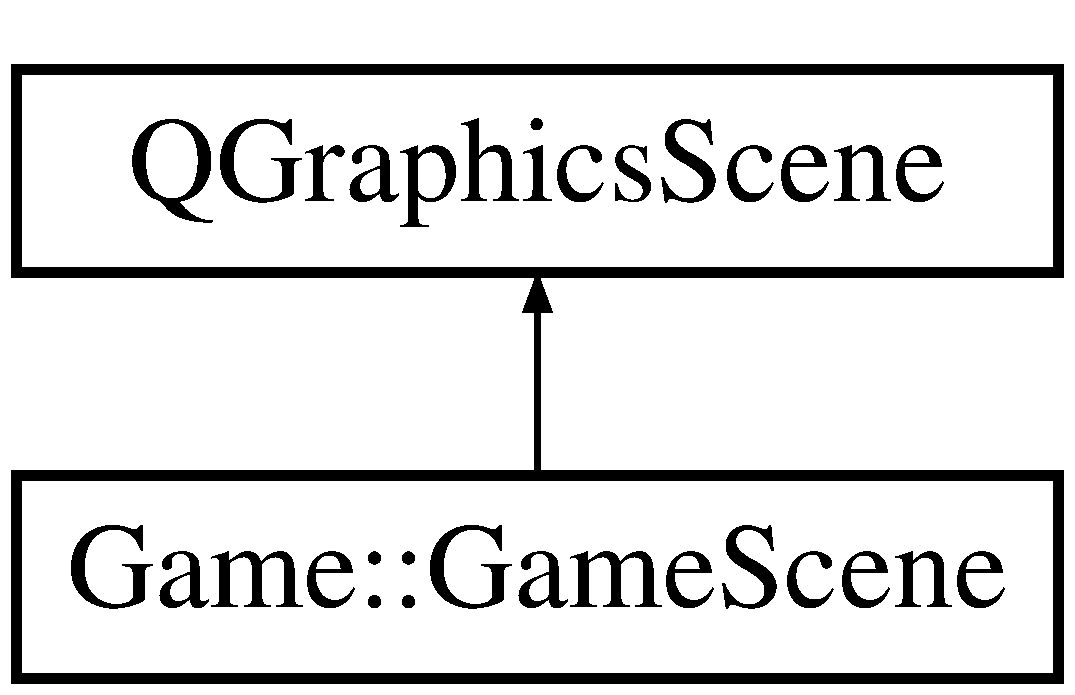
\includegraphics[height=2.000000cm]{classGame_1_1GameScene}
\end{center}
\end{figure}
\subsection*{Signals}
\begin{DoxyCompactItemize}
\item 
void \hyperlink{classGame_1_1GameScene_a9eafcdc42ec8c53bf01afb54c0a71316}{map\-Item\-Clicked} (\hyperlink{namespaceCourse_a9a16e743c9813da00109e4991afd2f3e}{Course\-::\-Object\-Id} id)
\begin{DoxyCompactList}\small\item\em signal that is triggered when a player clicks the map \end{DoxyCompactList}\end{DoxyCompactItemize}
\subsection*{Public Member Functions}
\begin{DoxyCompactItemize}
\item 
\hyperlink{classGame_1_1GameScene_a397788513ad96151c7fc3fc1642e5a53}{Game\-Scene} (Q\-Widget $\ast$qt\-\_\-parent=nullptr, int width=10, int height=10, int scale=50)
\begin{DoxyCompactList}\small\item\em Constructor for the class. \end{DoxyCompactList}\item 
\hyperlink{classGame_1_1GameScene_ac0ba459a7dd7671847247adf58dcf3b9}{$\sim$\-Game\-Scene} ()=default
\begin{DoxyCompactList}\small\item\em Default destructor. \end{DoxyCompactList}\item 
void \hyperlink{classGame_1_1GameScene_a94918fdf89d865606f1991e1a30d03f3}{set\-Size} (int width, int height)
\begin{DoxyCompactList}\small\item\em Sets the map size and calls \hyperlink{classGame_1_1GameScene_a855792a4b2ef6e6b1217a74806d0332c}{resize()}. \end{DoxyCompactList}\item 
void \hyperlink{classGame_1_1GameScene_a1687397ef51d1d8529fb76011dc14f96}{set\-Scale} (int scale)
\begin{DoxyCompactList}\small\item\em set the tile size, aka scale of the map and calls \hyperlink{classGame_1_1GameScene_a855792a4b2ef6e6b1217a74806d0332c}{resize()}. Function behaviour after objects has been drawn is not specified. \end{DoxyCompactList}\item 
void \hyperlink{classGame_1_1GameScene_a855792a4b2ef6e6b1217a74806d0332c}{resize} ()
\begin{DoxyCompactList}\small\item\em resize recalculates the bounding rectangle \end{DoxyCompactList}\item 
int \hyperlink{classGame_1_1GameScene_a12019298a905ba0a34324b9582b01477}{get\-Scale} () const 
\begin{DoxyCompactList}\small\item\em get the size of a single tile \end{DoxyCompactList}\item 
std\-::pair$<$ int, int $>$ \hyperlink{classGame_1_1GameScene_a37600217cb1b38b3188e40a52af166ff}{get\-Size} () const 
\begin{DoxyCompactList}\small\item\em get the size of the map. \end{DoxyCompactList}\item 
void \hyperlink{classGame_1_1GameScene_a1ec48db92996894288224918a9030790}{draw\-Item} (std\-::shared\-\_\-ptr$<$ \hyperlink{classCourse_1_1GameObject}{Course\-::\-Game\-Object} $>$ obj, int offset=0)
\begin{DoxyCompactList}\small\item\em draw a new item to the map. \end{DoxyCompactList}\item 
void \hyperlink{classGame_1_1GameScene_ad95d0d9226a3912889443a3c7bd80308}{remove\-Item} (std\-::shared\-\_\-ptr$<$ \hyperlink{classCourse_1_1GameObject}{Course\-::\-Game\-Object} $>$ obj)
\begin{DoxyCompactList}\small\item\em tries to remove drawn object at the location obj points to. If there's multiple objects, will remove the one that matches obj. \end{DoxyCompactList}\item 
void \hyperlink{classGame_1_1GameScene_ac0f74939076d910e28907cb26c6ae9c2}{update\-Item} (std\-::shared\-\_\-ptr$<$ \hyperlink{classCourse_1_1GameObject}{Course\-::\-Game\-Object} $>$ obj)
\begin{DoxyCompactList}\small\item\em updates the position of obj. \end{DoxyCompactList}\item 
virtual bool \hyperlink{classGame_1_1GameScene_a1d87227ccf428f158f848d44cad55b72}{event} (Q\-Event $\ast$event) override
\begin{DoxyCompactList}\small\item\em simple event handler that notifies when objects or the play area is clicked. \end{DoxyCompactList}\end{DoxyCompactItemize}
\subsection*{Private Attributes}
\begin{DoxyCompactItemize}
\item 
Q\-Graphics\-Item $\ast$ \hyperlink{classGame_1_1GameScene_ac6fd0bea8129c9b61b8418324f371e16}{m\-\_\-map\-Bound\-Rect}
\item 
int \hyperlink{classGame_1_1GameScene_aff9acff4c58359bddb14bffec789d78b}{m\-\_\-width}
\item 
int \hyperlink{classGame_1_1GameScene_a86406ae913fa1410adee082dcfa27486}{m\-\_\-height}
\item 
int \hyperlink{classGame_1_1GameScene_ab88ed80cd4feb3838bca9221a15b478f}{m\-\_\-scale}
\end{DoxyCompactItemize}


\subsection{Detailed Description}
The \hyperlink{classGame_1_1GameScene}{Game\-Scene} is a custom Q\-Graphics\-Scene that shows a simple rendering of the game map. 

\subsection{Constructor \& Destructor Documentation}
\hypertarget{classGame_1_1GameScene_a397788513ad96151c7fc3fc1642e5a53}{\index{Game\-::\-Game\-Scene@{Game\-::\-Game\-Scene}!Game\-Scene@{Game\-Scene}}
\index{Game\-Scene@{Game\-Scene}!Game::GameScene@{Game\-::\-Game\-Scene}}
\subsubsection[{Game\-Scene}]{\setlength{\rightskip}{0pt plus 5cm}Game\-::\-Game\-Scene\-::\-Game\-Scene (
\begin{DoxyParamCaption}
\item[{Q\-Widget $\ast$}]{qt\-\_\-parent = {\ttfamily nullptr}, }
\item[{int}]{width = {\ttfamily 10}, }
\item[{int}]{height = {\ttfamily 10}, }
\item[{int}]{scale = {\ttfamily 50}}
\end{DoxyParamCaption}
)}}\label{classGame_1_1GameScene_a397788513ad96151c7fc3fc1642e5a53}


Constructor for the class. 


\begin{DoxyParams}{Parameters}
{\em qt\-\_\-parent} & points to the parent object per Qt's parent-\/child-\/system. \\
\hline
{\em width} & in tiles for the game map. \\
\hline
{\em height} & in tiles for the game map. \\
\hline
{\em scale} & is the size in pixels of a single square tile.\\
\hline
\end{DoxyParams}
\begin{DoxyPrecond}{Precondition}
0 $<$ width $<$= 100 \&\& 0 $<$ height $<$= 100 \&\& 0 $<$ scale $<$= 500. Otherwise default values are used for the created object. 
\end{DoxyPrecond}
\hypertarget{classGame_1_1GameScene_ac0ba459a7dd7671847247adf58dcf3b9}{\index{Game\-::\-Game\-Scene@{Game\-::\-Game\-Scene}!$\sim$\-Game\-Scene@{$\sim$\-Game\-Scene}}
\index{$\sim$\-Game\-Scene@{$\sim$\-Game\-Scene}!Game::GameScene@{Game\-::\-Game\-Scene}}
\subsubsection[{$\sim$\-Game\-Scene}]{\setlength{\rightskip}{0pt plus 5cm}Game\-::\-Game\-Scene\-::$\sim$\-Game\-Scene (
\begin{DoxyParamCaption}
{}
\end{DoxyParamCaption}
)\hspace{0.3cm}{\ttfamily [default]}}}\label{classGame_1_1GameScene_ac0ba459a7dd7671847247adf58dcf3b9}


Default destructor. 



\subsection{Member Function Documentation}
\hypertarget{classGame_1_1GameScene_a1ec48db92996894288224918a9030790}{\index{Game\-::\-Game\-Scene@{Game\-::\-Game\-Scene}!draw\-Item@{draw\-Item}}
\index{draw\-Item@{draw\-Item}!Game::GameScene@{Game\-::\-Game\-Scene}}
\subsubsection[{draw\-Item}]{\setlength{\rightskip}{0pt plus 5cm}void Game\-::\-Game\-Scene\-::draw\-Item (
\begin{DoxyParamCaption}
\item[{std\-::shared\-\_\-ptr$<$ {\bf Course\-::\-Game\-Object} $>$}]{obj, }
\item[{int}]{offset = {\ttfamily 0}}
\end{DoxyParamCaption}
)}}\label{classGame_1_1GameScene_a1ec48db92996894288224918a9030790}


draw a new item to the map. 


\begin{DoxyParams}{Parameters}
{\em obj} & shared ptr to the object \\
\hline
{\em offset} & for the item in the tile \\
\hline
\end{DoxyParams}
\begin{DoxyPrecond}{Precondition}
obj must have a valid coordinate property. 
\end{DoxyPrecond}
\begin{DoxyPostcond}{Postcondition}
Exception guarantee\-: None 
\end{DoxyPostcond}
\hypertarget{classGame_1_1GameScene_a1d87227ccf428f158f848d44cad55b72}{\index{Game\-::\-Game\-Scene@{Game\-::\-Game\-Scene}!event@{event}}
\index{event@{event}!Game::GameScene@{Game\-::\-Game\-Scene}}
\subsubsection[{event}]{\setlength{\rightskip}{0pt plus 5cm}bool Game\-::\-Game\-Scene\-::event (
\begin{DoxyParamCaption}
\item[{Q\-Event $\ast$}]{event}
\end{DoxyParamCaption}
)\hspace{0.3cm}{\ttfamily [override]}, {\ttfamily [virtual]}}}\label{classGame_1_1GameScene_a1d87227ccf428f158f848d44cad55b72}


simple event handler that notifies when objects or the play area is clicked. 


\begin{DoxyParams}{Parameters}
{\em event} & that has happened. \\
\hline
\end{DoxyParams}
\begin{DoxyReturn}{Returns}
True\-: if event was handled in the handler. False\-: if the event handling was passed over. 
\end{DoxyReturn}
\hypertarget{classGame_1_1GameScene_a12019298a905ba0a34324b9582b01477}{\index{Game\-::\-Game\-Scene@{Game\-::\-Game\-Scene}!get\-Scale@{get\-Scale}}
\index{get\-Scale@{get\-Scale}!Game::GameScene@{Game\-::\-Game\-Scene}}
\subsubsection[{get\-Scale}]{\setlength{\rightskip}{0pt plus 5cm}int Game\-::\-Game\-Scene\-::get\-Scale (
\begin{DoxyParamCaption}
{}
\end{DoxyParamCaption}
) const}}\label{classGame_1_1GameScene_a12019298a905ba0a34324b9582b01477}


get the size of a single tile 

\begin{DoxyReturn}{Returns}
the size of a tile in pixels. 
\end{DoxyReturn}
\begin{DoxyPostcond}{Postcondition}
Exception guarantee\-: No-\/throw 
\end{DoxyPostcond}
\hypertarget{classGame_1_1GameScene_a37600217cb1b38b3188e40a52af166ff}{\index{Game\-::\-Game\-Scene@{Game\-::\-Game\-Scene}!get\-Size@{get\-Size}}
\index{get\-Size@{get\-Size}!Game::GameScene@{Game\-::\-Game\-Scene}}
\subsubsection[{get\-Size}]{\setlength{\rightskip}{0pt plus 5cm}std\-::pair$<$ int, int $>$ Game\-::\-Game\-Scene\-::get\-Size (
\begin{DoxyParamCaption}
{}
\end{DoxyParamCaption}
) const}}\label{classGame_1_1GameScene_a37600217cb1b38b3188e40a52af166ff}


get the size of the map. 

\begin{DoxyReturn}{Returns}
pair$<$width, height$>$ in tiles. 
\end{DoxyReturn}
\begin{DoxyPostcond}{Postcondition}
Exception guarantee\-: No-\/throw 
\end{DoxyPostcond}
\hypertarget{classGame_1_1GameScene_a9eafcdc42ec8c53bf01afb54c0a71316}{\index{Game\-::\-Game\-Scene@{Game\-::\-Game\-Scene}!map\-Item\-Clicked@{map\-Item\-Clicked}}
\index{map\-Item\-Clicked@{map\-Item\-Clicked}!Game::GameScene@{Game\-::\-Game\-Scene}}
\subsubsection[{map\-Item\-Clicked}]{\setlength{\rightskip}{0pt plus 5cm}void Game\-::\-Game\-Scene\-::map\-Item\-Clicked (
\begin{DoxyParamCaption}
\item[{{\bf Course\-::\-Object\-Id}}]{id}
\end{DoxyParamCaption}
)\hspace{0.3cm}{\ttfamily [signal]}}}\label{classGame_1_1GameScene_a9eafcdc42ec8c53bf01afb54c0a71316}


signal that is triggered when a player clicks the map 


\begin{DoxyParams}{Parameters}
{\em id} & of the tile that was clicked. \\
\hline
\end{DoxyParams}
\hypertarget{classGame_1_1GameScene_ad95d0d9226a3912889443a3c7bd80308}{\index{Game\-::\-Game\-Scene@{Game\-::\-Game\-Scene}!remove\-Item@{remove\-Item}}
\index{remove\-Item@{remove\-Item}!Game::GameScene@{Game\-::\-Game\-Scene}}
\subsubsection[{remove\-Item}]{\setlength{\rightskip}{0pt plus 5cm}void Game\-::\-Game\-Scene\-::remove\-Item (
\begin{DoxyParamCaption}
\item[{std\-::shared\-\_\-ptr$<$ {\bf Course\-::\-Game\-Object} $>$}]{obj}
\end{DoxyParamCaption}
)}}\label{classGame_1_1GameScene_ad95d0d9226a3912889443a3c7bd80308}


tries to remove drawn object at the location obj points to. If there's multiple objects, will remove the one that matches obj. 


\begin{DoxyParams}{Parameters}
{\em obj} & shared ptr to the object being deleted. \\
\hline
\end{DoxyParams}
\begin{DoxyPostcond}{Postcondition}
Exception guarantee\-: None 
\end{DoxyPostcond}
\hypertarget{classGame_1_1GameScene_a855792a4b2ef6e6b1217a74806d0332c}{\index{Game\-::\-Game\-Scene@{Game\-::\-Game\-Scene}!resize@{resize}}
\index{resize@{resize}!Game::GameScene@{Game\-::\-Game\-Scene}}
\subsubsection[{resize}]{\setlength{\rightskip}{0pt plus 5cm}void Game\-::\-Game\-Scene\-::resize (
\begin{DoxyParamCaption}
{}
\end{DoxyParamCaption}
)}}\label{classGame_1_1GameScene_a855792a4b2ef6e6b1217a74806d0332c}


resize recalculates the bounding rectangle 

\hypertarget{classGame_1_1GameScene_a1687397ef51d1d8529fb76011dc14f96}{\index{Game\-::\-Game\-Scene@{Game\-::\-Game\-Scene}!set\-Scale@{set\-Scale}}
\index{set\-Scale@{set\-Scale}!Game::GameScene@{Game\-::\-Game\-Scene}}
\subsubsection[{set\-Scale}]{\setlength{\rightskip}{0pt plus 5cm}void Game\-::\-Game\-Scene\-::set\-Scale (
\begin{DoxyParamCaption}
\item[{int}]{scale}
\end{DoxyParamCaption}
)}}\label{classGame_1_1GameScene_a1687397ef51d1d8529fb76011dc14f96}


set the tile size, aka scale of the map and calls \hyperlink{classGame_1_1GameScene_a855792a4b2ef6e6b1217a74806d0332c}{resize()}. Function behaviour after objects has been drawn is not specified. 


\begin{DoxyParams}{Parameters}
{\em scale} & in pixels. \\
\hline
\end{DoxyParams}
\begin{DoxyPrecond}{Precondition}
0 $<$ scale $<$= 500 
\end{DoxyPrecond}
\begin{DoxyPostcond}{Postcondition}
Scene scale is set to scale. 

Exception guarantee\-: None 
\end{DoxyPostcond}
\hypertarget{classGame_1_1GameScene_a94918fdf89d865606f1991e1a30d03f3}{\index{Game\-::\-Game\-Scene@{Game\-::\-Game\-Scene}!set\-Size@{set\-Size}}
\index{set\-Size@{set\-Size}!Game::GameScene@{Game\-::\-Game\-Scene}}
\subsubsection[{set\-Size}]{\setlength{\rightskip}{0pt plus 5cm}void Game\-::\-Game\-Scene\-::set\-Size (
\begin{DoxyParamCaption}
\item[{int}]{width, }
\item[{int}]{height}
\end{DoxyParamCaption}
)}}\label{classGame_1_1GameScene_a94918fdf89d865606f1991e1a30d03f3}


Sets the map size and calls \hyperlink{classGame_1_1GameScene_a855792a4b2ef6e6b1217a74806d0332c}{resize()}. 


\begin{DoxyParams}{Parameters}
{\em width} & in tiles. \\
\hline
{\em height} & in tiles. \\
\hline
\end{DoxyParams}
\begin{DoxyPrecond}{Precondition}
width and height must each be between 1 and 100. 
\end{DoxyPrecond}
\begin{DoxyPostcond}{Postcondition}
width and height are set to given sizes. 

Exception guarantee\-: No-\/throw 
\end{DoxyPostcond}
\hypertarget{classGame_1_1GameScene_ac0f74939076d910e28907cb26c6ae9c2}{\index{Game\-::\-Game\-Scene@{Game\-::\-Game\-Scene}!update\-Item@{update\-Item}}
\index{update\-Item@{update\-Item}!Game::GameScene@{Game\-::\-Game\-Scene}}
\subsubsection[{update\-Item}]{\setlength{\rightskip}{0pt plus 5cm}void Game\-::\-Game\-Scene\-::update\-Item (
\begin{DoxyParamCaption}
\item[{std\-::shared\-\_\-ptr$<$ {\bf Course\-::\-Game\-Object} $>$}]{obj}
\end{DoxyParamCaption}
)}}\label{classGame_1_1GameScene_ac0f74939076d910e28907cb26c6ae9c2}


updates the position of obj. 


\begin{DoxyParams}{Parameters}
{\em obj} & shared ptr to the obj being updated. \\
\hline
\end{DoxyParams}


\subsection{Member Data Documentation}
\hypertarget{classGame_1_1GameScene_a86406ae913fa1410adee082dcfa27486}{\index{Game\-::\-Game\-Scene@{Game\-::\-Game\-Scene}!m\-\_\-height@{m\-\_\-height}}
\index{m\-\_\-height@{m\-\_\-height}!Game::GameScene@{Game\-::\-Game\-Scene}}
\subsubsection[{m\-\_\-height}]{\setlength{\rightskip}{0pt plus 5cm}int Game\-::\-Game\-Scene\-::m\-\_\-height\hspace{0.3cm}{\ttfamily [private]}}}\label{classGame_1_1GameScene_a86406ae913fa1410adee082dcfa27486}
\hypertarget{classGame_1_1GameScene_ac6fd0bea8129c9b61b8418324f371e16}{\index{Game\-::\-Game\-Scene@{Game\-::\-Game\-Scene}!m\-\_\-map\-Bound\-Rect@{m\-\_\-map\-Bound\-Rect}}
\index{m\-\_\-map\-Bound\-Rect@{m\-\_\-map\-Bound\-Rect}!Game::GameScene@{Game\-::\-Game\-Scene}}
\subsubsection[{m\-\_\-map\-Bound\-Rect}]{\setlength{\rightskip}{0pt plus 5cm}Q\-Graphics\-Item$\ast$ Game\-::\-Game\-Scene\-::m\-\_\-map\-Bound\-Rect\hspace{0.3cm}{\ttfamily [private]}}}\label{classGame_1_1GameScene_ac6fd0bea8129c9b61b8418324f371e16}
\hypertarget{classGame_1_1GameScene_ab88ed80cd4feb3838bca9221a15b478f}{\index{Game\-::\-Game\-Scene@{Game\-::\-Game\-Scene}!m\-\_\-scale@{m\-\_\-scale}}
\index{m\-\_\-scale@{m\-\_\-scale}!Game::GameScene@{Game\-::\-Game\-Scene}}
\subsubsection[{m\-\_\-scale}]{\setlength{\rightskip}{0pt plus 5cm}int Game\-::\-Game\-Scene\-::m\-\_\-scale\hspace{0.3cm}{\ttfamily [private]}}}\label{classGame_1_1GameScene_ab88ed80cd4feb3838bca9221a15b478f}
\hypertarget{classGame_1_1GameScene_aff9acff4c58359bddb14bffec789d78b}{\index{Game\-::\-Game\-Scene@{Game\-::\-Game\-Scene}!m\-\_\-width@{m\-\_\-width}}
\index{m\-\_\-width@{m\-\_\-width}!Game::GameScene@{Game\-::\-Game\-Scene}}
\subsubsection[{m\-\_\-width}]{\setlength{\rightskip}{0pt plus 5cm}int Game\-::\-Game\-Scene\-::m\-\_\-width\hspace{0.3cm}{\ttfamily [private]}}}\label{classGame_1_1GameScene_aff9acff4c58359bddb14bffec789d78b}


The documentation for this class was generated from the following files\-:\begin{DoxyCompactItemize}
\item 
Game/graphics/\hyperlink{gamescene_8h}{gamescene.\-h}\item 
Game/graphics/\hyperlink{gamescene_8cpp}{gamescene.\-cpp}\end{DoxyCompactItemize}

\hypertarget{classCourse_1_1Grassland}{\section{Course\-:\-:Grassland Class Reference}
\label{classCourse_1_1Grassland}\index{Course\-::\-Grassland@{Course\-::\-Grassland}}
}


The \hyperlink{classCourse_1_1Grassland}{Grassland} class represents \hyperlink{classCourse_1_1Grassland}{Grassland} in the gameworld.  




{\ttfamily \#include $<$grassland.\-h$>$}

Inheritance diagram for Course\-:\-:Grassland\-:\begin{figure}[H]
\begin{center}
\leavevmode
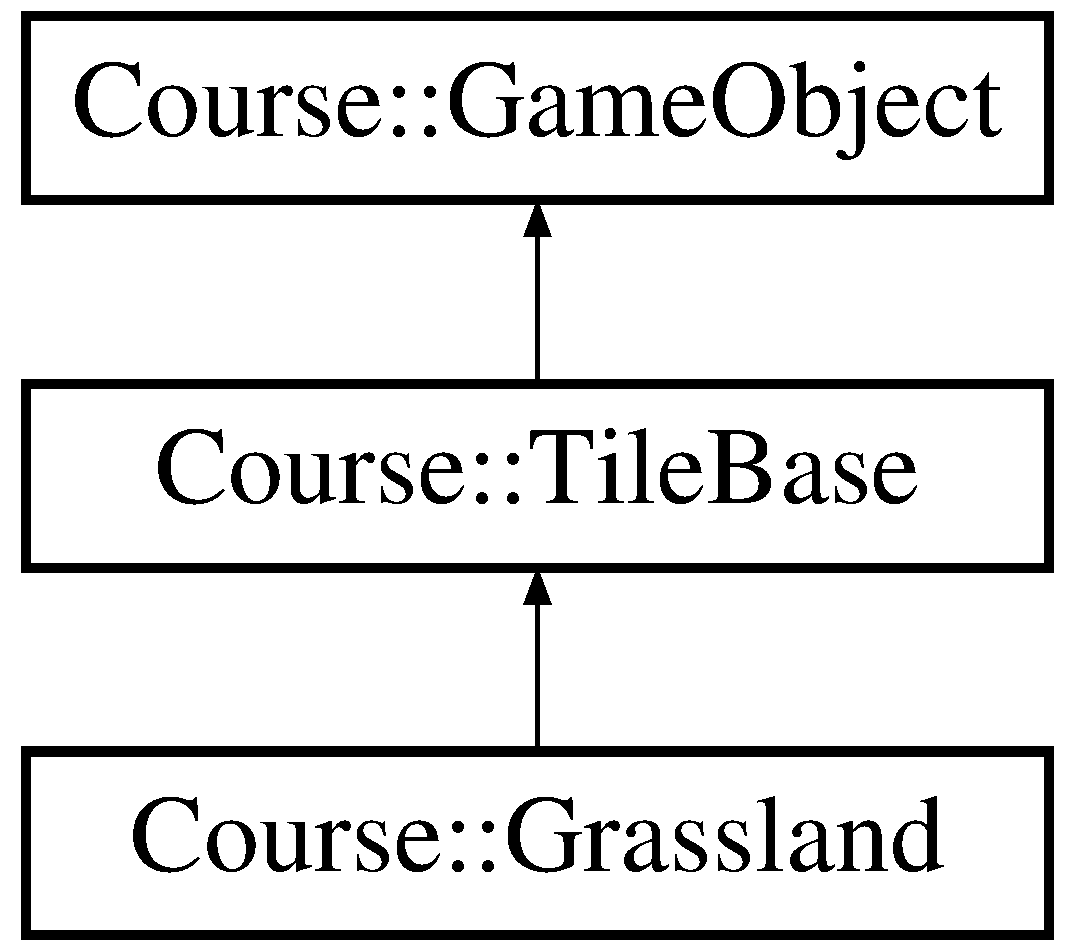
\includegraphics[height=3.000000cm]{classCourse_1_1Grassland}
\end{center}
\end{figure}
\subsection*{Public Member Functions}
\begin{DoxyCompactItemize}
\item 
\hyperlink{classCourse_1_1Grassland_a1263204b4995f7306d9a78c5769e30c0}{Grassland} ()=delete
\begin{DoxyCompactList}\small\item\em Disabled parameterless constructor. \end{DoxyCompactList}\item 
\hyperlink{classCourse_1_1Grassland_a8d7239afef39efc0531c74ece6ecdc67}{Grassland} (const \hyperlink{classCourse_1_1Coordinate}{Coordinate} \&location, const std\-::shared\-\_\-ptr$<$ \hyperlink{classCourse_1_1iGameEventHandler}{i\-Game\-Event\-Handler} $>$ \&eventhandler, const std\-::shared\-\_\-ptr$<$ \hyperlink{classCourse_1_1iObjectManager}{i\-Object\-Manager} $>$ \&objectmanager, const unsigned int \&max\-\_\-build=3, const unsigned int \&max\-\_\-work=3, const \hyperlink{namespaceCourse_ab9a46ed9cd00485e318e5731ea2f78d9}{Resource\-Map} \&production=\hyperlink{namespaceCourse_1_1ConstResourceMaps_aae4ef780a53ec4726ff947ecae010082}{Const\-Resource\-Maps\-::\-G\-R\-A\-S\-S\-L\-A\-N\-D\-\_\-\-B\-P})
\begin{DoxyCompactList}\small\item\em Constructor for the class. \end{DoxyCompactList}\item 
virtual \hyperlink{classCourse_1_1Grassland_aa660837530ab2dcc563c9557ec599066}{$\sim$\-Grassland} ()=default
\begin{DoxyCompactList}\small\item\em Default destructor. \end{DoxyCompactList}\item 
virtual std\-::string \hyperlink{classCourse_1_1Grassland_a0a652bbecdda0216613dad980936e30e}{get\-Type} () const override
\begin{DoxyCompactList}\small\item\em get\-Type Returns a string describing objects type. This should be overriden in each inherited class. Makes checking object's type easier for students. \end{DoxyCompactList}\end{DoxyCompactItemize}
\subsection*{Static Public Attributes}
\begin{DoxyCompactItemize}
\item 
static const unsigned int \hyperlink{classCourse_1_1Grassland_aa90f673331e9c748a5960c513c27cdd9}{M\-A\-X\-\_\-\-B\-U\-I\-L\-D\-I\-N\-G\-S}
\item 
static const unsigned int \hyperlink{classCourse_1_1Grassland_af92733b817010370c0540d1631b6f486}{M\-A\-X\-\_\-\-W\-O\-R\-K\-E\-R\-S}
\item 
static const \hyperlink{namespaceCourse_ab9a46ed9cd00485e318e5731ea2f78d9}{Resource\-Map} \hyperlink{classCourse_1_1Grassland_a35a3ec14967c6b7446caa94887e33524}{B\-A\-S\-E\-\_\-\-P\-R\-O\-D\-U\-C\-T\-I\-O\-N}
\end{DoxyCompactItemize}
\subsection*{Additional Inherited Members}


\subsection{Detailed Description}
The \hyperlink{classCourse_1_1Grassland}{Grassland} class represents \hyperlink{classCourse_1_1Grassland}{Grassland} in the gameworld. 

\hyperlink{classCourse_1_1Grassland}{Grassland} has Basic\-Production\-: \par

\begin{DoxyItemize}
\item Money = 2
\item Food = 5
\item Wood = 1
\item Stone = 1
\item Ore = 0
\end{DoxyItemize}

Functionality follows mainly the parent class' functionality.

Tile supports 3 buildings. 

\subsection{Constructor \& Destructor Documentation}
\hypertarget{classCourse_1_1Grassland_a1263204b4995f7306d9a78c5769e30c0}{\index{Course\-::\-Grassland@{Course\-::\-Grassland}!Grassland@{Grassland}}
\index{Grassland@{Grassland}!Course::Grassland@{Course\-::\-Grassland}}
\subsubsection[{Grassland}]{\setlength{\rightskip}{0pt plus 5cm}Course\-::\-Grassland\-::\-Grassland (
\begin{DoxyParamCaption}
{}
\end{DoxyParamCaption}
)\hspace{0.3cm}{\ttfamily [delete]}}}\label{classCourse_1_1Grassland_a1263204b4995f7306d9a78c5769e30c0}


Disabled parameterless constructor. 

\hypertarget{classCourse_1_1Grassland_a8d7239afef39efc0531c74ece6ecdc67}{\index{Course\-::\-Grassland@{Course\-::\-Grassland}!Grassland@{Grassland}}
\index{Grassland@{Grassland}!Course::Grassland@{Course\-::\-Grassland}}
\subsubsection[{Grassland}]{\setlength{\rightskip}{0pt plus 5cm}Course\-::\-Grassland\-::\-Grassland (
\begin{DoxyParamCaption}
\item[{const {\bf Coordinate} \&}]{location, }
\item[{const std\-::shared\-\_\-ptr$<$ {\bf i\-Game\-Event\-Handler} $>$ \&}]{eventhandler, }
\item[{const std\-::shared\-\_\-ptr$<$ {\bf i\-Object\-Manager} $>$ \&}]{objectmanager, }
\item[{const unsigned int \&}]{max\-\_\-build = {\ttfamily 3}, }
\item[{const unsigned int \&}]{max\-\_\-work = {\ttfamily 3}, }
\item[{const {\bf Resource\-Map} \&}]{production = {\ttfamily {\bf Const\-Resource\-Maps\-::\-G\-R\-A\-S\-S\-L\-A\-N\-D\-\_\-\-B\-P}}}
\end{DoxyParamCaption}
)}}\label{classCourse_1_1Grassland_a8d7239afef39efc0531c74ece6ecdc67}


Constructor for the class. 


\begin{DoxyParams}{Parameters}
{\em location} & is the \hyperlink{classCourse_1_1Coordinate}{Coordinate} where the Tile is located in the game. \\
\hline
{\em eventhandler} & points to the student's Game\-Event\-Handler. \\
\hline
\end{DoxyParams}
\hypertarget{classCourse_1_1Grassland_aa660837530ab2dcc563c9557ec599066}{\index{Course\-::\-Grassland@{Course\-::\-Grassland}!$\sim$\-Grassland@{$\sim$\-Grassland}}
\index{$\sim$\-Grassland@{$\sim$\-Grassland}!Course::Grassland@{Course\-::\-Grassland}}
\subsubsection[{$\sim$\-Grassland}]{\setlength{\rightskip}{0pt plus 5cm}virtual Course\-::\-Grassland\-::$\sim$\-Grassland (
\begin{DoxyParamCaption}
{}
\end{DoxyParamCaption}
)\hspace{0.3cm}{\ttfamily [virtual]}, {\ttfamily [default]}}}\label{classCourse_1_1Grassland_aa660837530ab2dcc563c9557ec599066}


Default destructor. 



\subsection{Member Function Documentation}
\hypertarget{classCourse_1_1Grassland_a0a652bbecdda0216613dad980936e30e}{\index{Course\-::\-Grassland@{Course\-::\-Grassland}!get\-Type@{get\-Type}}
\index{get\-Type@{get\-Type}!Course::Grassland@{Course\-::\-Grassland}}
\subsubsection[{get\-Type}]{\setlength{\rightskip}{0pt plus 5cm}std\-::string Course\-::\-Grassland\-::get\-Type (
\begin{DoxyParamCaption}
{}
\end{DoxyParamCaption}
) const\hspace{0.3cm}{\ttfamily [override]}, {\ttfamily [virtual]}}}\label{classCourse_1_1Grassland_a0a652bbecdda0216613dad980936e30e}


get\-Type Returns a string describing objects type. This should be overriden in each inherited class. Makes checking object's type easier for students. 

\begin{DoxyReturn}{Returns}
std\-::string that represents Object's type. 
\end{DoxyReturn}
\begin{DoxyPostcond}{Postcondition}
Exception guarantee\-: No-\/throw 
\end{DoxyPostcond}
\begin{DoxyNote}{Note}
You can use this in e.\-g. debugging and similar printing. 
\end{DoxyNote}


Reimplemented from \hyperlink{classCourse_1_1TileBase_af1a8aaa3407ad3ade7ffe8f2fb421288}{Course\-::\-Tile\-Base}.



\subsection{Member Data Documentation}
\hypertarget{classCourse_1_1Grassland_a35a3ec14967c6b7446caa94887e33524}{\index{Course\-::\-Grassland@{Course\-::\-Grassland}!B\-A\-S\-E\-\_\-\-P\-R\-O\-D\-U\-C\-T\-I\-O\-N@{B\-A\-S\-E\-\_\-\-P\-R\-O\-D\-U\-C\-T\-I\-O\-N}}
\index{B\-A\-S\-E\-\_\-\-P\-R\-O\-D\-U\-C\-T\-I\-O\-N@{B\-A\-S\-E\-\_\-\-P\-R\-O\-D\-U\-C\-T\-I\-O\-N}!Course::Grassland@{Course\-::\-Grassland}}
\subsubsection[{B\-A\-S\-E\-\_\-\-P\-R\-O\-D\-U\-C\-T\-I\-O\-N}]{\setlength{\rightskip}{0pt plus 5cm}const {\bf Resource\-Map} Course\-::\-Grassland\-::\-B\-A\-S\-E\-\_\-\-P\-R\-O\-D\-U\-C\-T\-I\-O\-N\hspace{0.3cm}{\ttfamily [static]}}}\label{classCourse_1_1Grassland_a35a3ec14967c6b7446caa94887e33524}
\hypertarget{classCourse_1_1Grassland_aa90f673331e9c748a5960c513c27cdd9}{\index{Course\-::\-Grassland@{Course\-::\-Grassland}!M\-A\-X\-\_\-\-B\-U\-I\-L\-D\-I\-N\-G\-S@{M\-A\-X\-\_\-\-B\-U\-I\-L\-D\-I\-N\-G\-S}}
\index{M\-A\-X\-\_\-\-B\-U\-I\-L\-D\-I\-N\-G\-S@{M\-A\-X\-\_\-\-B\-U\-I\-L\-D\-I\-N\-G\-S}!Course::Grassland@{Course\-::\-Grassland}}
\subsubsection[{M\-A\-X\-\_\-\-B\-U\-I\-L\-D\-I\-N\-G\-S}]{\setlength{\rightskip}{0pt plus 5cm}const unsigned int Course\-::\-Grassland\-::\-M\-A\-X\-\_\-\-B\-U\-I\-L\-D\-I\-N\-G\-S\hspace{0.3cm}{\ttfamily [static]}}}\label{classCourse_1_1Grassland_aa90f673331e9c748a5960c513c27cdd9}
\hypertarget{classCourse_1_1Grassland_af92733b817010370c0540d1631b6f486}{\index{Course\-::\-Grassland@{Course\-::\-Grassland}!M\-A\-X\-\_\-\-W\-O\-R\-K\-E\-R\-S@{M\-A\-X\-\_\-\-W\-O\-R\-K\-E\-R\-S}}
\index{M\-A\-X\-\_\-\-W\-O\-R\-K\-E\-R\-S@{M\-A\-X\-\_\-\-W\-O\-R\-K\-E\-R\-S}!Course::Grassland@{Course\-::\-Grassland}}
\subsubsection[{M\-A\-X\-\_\-\-W\-O\-R\-K\-E\-R\-S}]{\setlength{\rightskip}{0pt plus 5cm}const unsigned int Course\-::\-Grassland\-::\-M\-A\-X\-\_\-\-W\-O\-R\-K\-E\-R\-S\hspace{0.3cm}{\ttfamily [static]}}}\label{classCourse_1_1Grassland_af92733b817010370c0540d1631b6f486}


The documentation for this class was generated from the following files\-:\begin{DoxyCompactItemize}
\item 
Course/\-Course\-Lib/tiles/\hyperlink{grassland_8h}{grassland.\-h}\item 
Course/\-Course\-Lib/tiles/\hyperlink{grassland_8cpp}{grassland.\-cpp}\end{DoxyCompactItemize}

\hypertarget{classCourse_1_1HeadQuarters}{\section{Course\-:\-:Head\-Quarters Class Reference}
\label{classCourse_1_1HeadQuarters}\index{Course\-::\-Head\-Quarters@{Course\-::\-Head\-Quarters}}
}


The \hyperlink{classCourse_1_1HeadQuarters}{Head\-Quarters} class represents a player's Head\-Quarters-\/building.  




{\ttfamily \#include $<$headquarters.\-h$>$}

Inheritance diagram for Course\-:\-:Head\-Quarters\-:\begin{figure}[H]
\begin{center}
\leavevmode
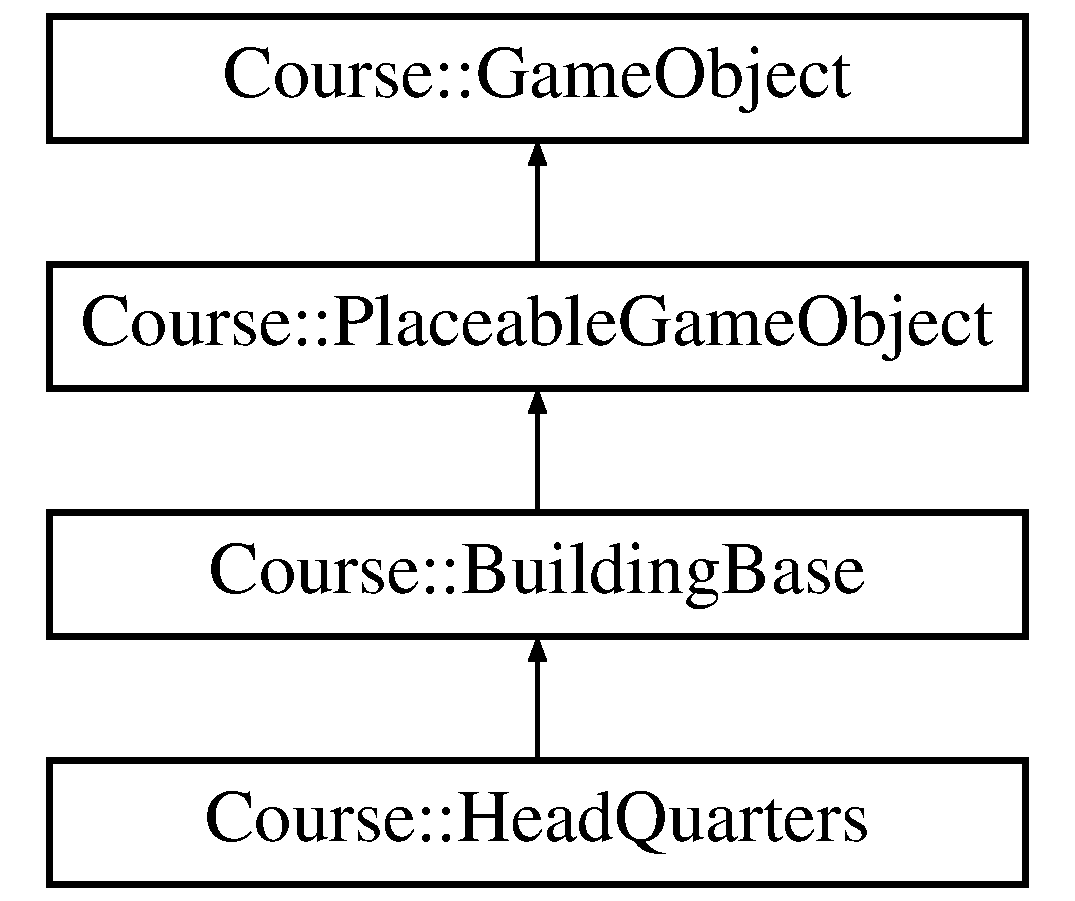
\includegraphics[height=4.000000cm]{classCourse_1_1HeadQuarters}
\end{center}
\end{figure}
\subsection*{Public Member Functions}
\begin{DoxyCompactItemize}
\item 
\hyperlink{classCourse_1_1HeadQuarters_a117d344b8498b5fee8da099d5f3c06a5}{Head\-Quarters} ()=delete
\begin{DoxyCompactList}\small\item\em Disabled parameterless constructor. \end{DoxyCompactList}\item 
\hyperlink{classCourse_1_1HeadQuarters_a7c928678452102770fff5d0e5ad1bdf9}{Head\-Quarters} (const std\-::shared\-\_\-ptr$<$ \hyperlink{classCourse_1_1iGameEventHandler}{i\-Game\-Event\-Handler} $>$ \&eventhandler, const std\-::shared\-\_\-ptr$<$ \hyperlink{classCourse_1_1iObjectManager}{i\-Object\-Manager} $>$ \&objectmanager, const std\-::shared\-\_\-ptr$<$ \hyperlink{classCourse_1_1PlayerBase}{Player\-Base} $>$ \&owner, const int \&tilespaces=1, const \hyperlink{namespaceCourse_ab9a46ed9cd00485e318e5731ea2f78d9}{Resource\-Map} \&buildcost=\hyperlink{namespaceCourse_1_1ConstResourceMaps_a629a12b3f9357cd851c54f2126d22502}{Const\-Resource\-Maps\-::\-H\-Q\-\_\-\-B\-U\-I\-L\-D\-\_\-\-C\-O\-S\-T}, const \hyperlink{namespaceCourse_ab9a46ed9cd00485e318e5731ea2f78d9}{Resource\-Map} \&production=\hyperlink{namespaceCourse_1_1ConstResourceMaps_aabaaa4f78c30eed6e966b596423c8dea}{Const\-Resource\-Maps\-::\-H\-Q\-\_\-\-P\-R\-O\-D\-U\-C\-T\-I\-O\-N})
\begin{DoxyCompactList}\small\item\em Constructor for the class. \end{DoxyCompactList}\item 
virtual \hyperlink{classCourse_1_1HeadQuarters_afb7c412b1d0a4997a90c87940de2eabd}{$\sim$\-Head\-Quarters} ()=default
\begin{DoxyCompactList}\small\item\em Default destructor. \end{DoxyCompactList}\item 
virtual std\-::string \hyperlink{classCourse_1_1HeadQuarters_a1d9a996a6a87ca31aeb63dff2d41d242}{get\-Type} () const override
\begin{DoxyCompactList}\small\item\em get\-Type Returns a string describing objects type. This should be overriden in each inherited class. Makes checking object's type easier for students. \end{DoxyCompactList}\item 
virtual void \hyperlink{classCourse_1_1HeadQuarters_addf7f7f78486ce17024a639f15f25649}{on\-Build\-Action} () override
\begin{DoxyCompactList}\small\item\em Sets neighbouring Tiles' ownership to this building's ownership in 3 tile-\/radius, if the Tiles don't already have an owner. \end{DoxyCompactList}\end{DoxyCompactItemize}
\subsection*{Additional Inherited Members}


\subsection{Detailed Description}
The \hyperlink{classCourse_1_1HeadQuarters}{Head\-Quarters} class represents a player's Head\-Quarters-\/building. 

It can be constructed on any tile that has not been claimed by any other player. \par
Effects\-: Claims surrounding unclaimed tiles. \par
Radius\-: 3 tiles. 

\subsection{Constructor \& Destructor Documentation}
\hypertarget{classCourse_1_1HeadQuarters_a117d344b8498b5fee8da099d5f3c06a5}{\index{Course\-::\-Head\-Quarters@{Course\-::\-Head\-Quarters}!Head\-Quarters@{Head\-Quarters}}
\index{Head\-Quarters@{Head\-Quarters}!Course::HeadQuarters@{Course\-::\-Head\-Quarters}}
\subsubsection[{Head\-Quarters}]{\setlength{\rightskip}{0pt plus 5cm}Course\-::\-Head\-Quarters\-::\-Head\-Quarters (
\begin{DoxyParamCaption}
{}
\end{DoxyParamCaption}
)\hspace{0.3cm}{\ttfamily [delete]}}}\label{classCourse_1_1HeadQuarters_a117d344b8498b5fee8da099d5f3c06a5}


Disabled parameterless constructor. 

\hypertarget{classCourse_1_1HeadQuarters_a7c928678452102770fff5d0e5ad1bdf9}{\index{Course\-::\-Head\-Quarters@{Course\-::\-Head\-Quarters}!Head\-Quarters@{Head\-Quarters}}
\index{Head\-Quarters@{Head\-Quarters}!Course::HeadQuarters@{Course\-::\-Head\-Quarters}}
\subsubsection[{Head\-Quarters}]{\setlength{\rightskip}{0pt plus 5cm}Course\-::\-Head\-Quarters\-::\-Head\-Quarters (
\begin{DoxyParamCaption}
\item[{const std\-::shared\-\_\-ptr$<$ {\bf i\-Game\-Event\-Handler} $>$ \&}]{eventhandler, }
\item[{const std\-::shared\-\_\-ptr$<$ {\bf i\-Object\-Manager} $>$ \&}]{objectmanager, }
\item[{const std\-::shared\-\_\-ptr$<$ {\bf Player\-Base} $>$ \&}]{owner, }
\item[{const int \&}]{tilespaces = {\ttfamily 1}, }
\item[{const {\bf Resource\-Map} \&}]{buildcost = {\ttfamily {\bf Const\-Resource\-Maps\-::\-H\-Q\-\_\-\-B\-U\-I\-L\-D\-\_\-\-C\-O\-S\-T}}, }
\item[{const {\bf Resource\-Map} \&}]{production = {\ttfamily {\bf Const\-Resource\-Maps\-::\-H\-Q\-\_\-\-P\-R\-O\-D\-U\-C\-T\-I\-O\-N}}}
\end{DoxyParamCaption}
)\hspace{0.3cm}{\ttfamily [explicit]}}}\label{classCourse_1_1HeadQuarters_a7c928678452102770fff5d0e5ad1bdf9}


Constructor for the class. 


\begin{DoxyParams}{Parameters}
{\em eventhandler} & points to the student's Game\-Event\-Handler. \\
\hline
{\em owner} & points to the owning player. \\
\hline
{\em tile} & points to the tile upon which the building is constructed.\\
\hline
\end{DoxyParams}
\begin{DoxyPostcond}{Postcondition}
Exception Guarantee\-: No guarantee. 
\end{DoxyPostcond}

\begin{DoxyExceptions}{Exceptions}
{\em \hyperlink{classCourse_1_1OwnerConflict}{Owner\-Conflict}} & -\/ if the building conflicts with tile's ownership. \\
\hline
\end{DoxyExceptions}
\hypertarget{classCourse_1_1HeadQuarters_afb7c412b1d0a4997a90c87940de2eabd}{\index{Course\-::\-Head\-Quarters@{Course\-::\-Head\-Quarters}!$\sim$\-Head\-Quarters@{$\sim$\-Head\-Quarters}}
\index{$\sim$\-Head\-Quarters@{$\sim$\-Head\-Quarters}!Course::HeadQuarters@{Course\-::\-Head\-Quarters}}
\subsubsection[{$\sim$\-Head\-Quarters}]{\setlength{\rightskip}{0pt plus 5cm}virtual Course\-::\-Head\-Quarters\-::$\sim$\-Head\-Quarters (
\begin{DoxyParamCaption}
{}
\end{DoxyParamCaption}
)\hspace{0.3cm}{\ttfamily [virtual]}, {\ttfamily [default]}}}\label{classCourse_1_1HeadQuarters_afb7c412b1d0a4997a90c87940de2eabd}


Default destructor. 



\subsection{Member Function Documentation}
\hypertarget{classCourse_1_1HeadQuarters_a1d9a996a6a87ca31aeb63dff2d41d242}{\index{Course\-::\-Head\-Quarters@{Course\-::\-Head\-Quarters}!get\-Type@{get\-Type}}
\index{get\-Type@{get\-Type}!Course::HeadQuarters@{Course\-::\-Head\-Quarters}}
\subsubsection[{get\-Type}]{\setlength{\rightskip}{0pt plus 5cm}std\-::string Course\-::\-Head\-Quarters\-::get\-Type (
\begin{DoxyParamCaption}
{}
\end{DoxyParamCaption}
) const\hspace{0.3cm}{\ttfamily [override]}, {\ttfamily [virtual]}}}\label{classCourse_1_1HeadQuarters_a1d9a996a6a87ca31aeb63dff2d41d242}


get\-Type Returns a string describing objects type. This should be overriden in each inherited class. Makes checking object's type easier for students. 

\begin{DoxyReturn}{Returns}
std\-::string that represents Object's type. 
\end{DoxyReturn}
\begin{DoxyPostcond}{Postcondition}
Exception guarantee\-: No-\/throw 
\end{DoxyPostcond}
\begin{DoxyNote}{Note}
You can use this in e.\-g. debugging and similar printing. 
\end{DoxyNote}


Reimplemented from \hyperlink{classCourse_1_1BuildingBase_ac2cc44e08dc73d05b1617bf71295baaf}{Course\-::\-Building\-Base}.

\hypertarget{classCourse_1_1HeadQuarters_addf7f7f78486ce17024a639f15f25649}{\index{Course\-::\-Head\-Quarters@{Course\-::\-Head\-Quarters}!on\-Build\-Action@{on\-Build\-Action}}
\index{on\-Build\-Action@{on\-Build\-Action}!Course::HeadQuarters@{Course\-::\-Head\-Quarters}}
\subsubsection[{on\-Build\-Action}]{\setlength{\rightskip}{0pt plus 5cm}void Course\-::\-Head\-Quarters\-::on\-Build\-Action (
\begin{DoxyParamCaption}
{}
\end{DoxyParamCaption}
)\hspace{0.3cm}{\ttfamily [override]}, {\ttfamily [virtual]}}}\label{classCourse_1_1HeadQuarters_addf7f7f78486ce17024a639f15f25649}


Sets neighbouring Tiles' ownership to this building's ownership in 3 tile-\/radius, if the Tiles don't already have an owner. 

\begin{DoxyPostcond}{Postcondition}
Exception guarantee\-: Basic 
\end{DoxyPostcond}


Reimplemented from \hyperlink{classCourse_1_1BuildingBase_a2e3a5ad53afb74fdf030a5679e40a341}{Course\-::\-Building\-Base}.



The documentation for this class was generated from the following files\-:\begin{DoxyCompactItemize}
\item 
Course/\-Course\-Lib/buildings/\hyperlink{headquarters_8h}{headquarters.\-h}\item 
Course/\-Course\-Lib/buildings/\hyperlink{headquarters_8cpp}{headquarters.\-cpp}\end{DoxyCompactItemize}

\hypertarget{classCourse_1_1iGameEventHandler}{\section{Course\-:\-:i\-Game\-Event\-Handler Class Reference}
\label{classCourse_1_1iGameEventHandler}\index{Course\-::i\-Game\-Event\-Handler@{Course\-::i\-Game\-Event\-Handler}}
}


The \hyperlink{classCourse_1_1iGameEventHandler}{i\-Game\-Event\-Handler} class is an interface which the Course-\/side code uses to interact with the Game\-Event\-Handler implemented by the students.  




{\ttfamily \#include $<$igameeventhandler.\-h$>$}

Inheritance diagram for Course\-:\-:i\-Game\-Event\-Handler\-:\begin{figure}[H]
\begin{center}
\leavevmode
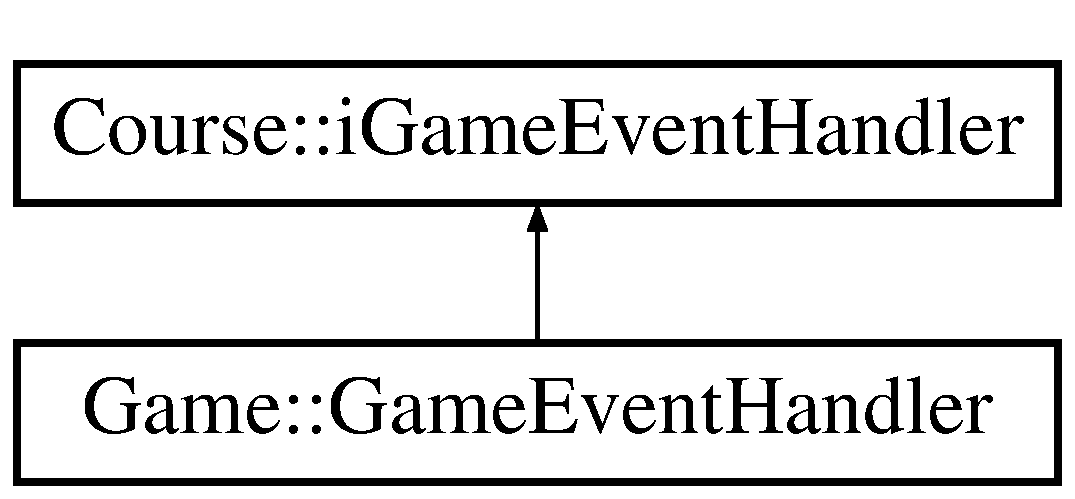
\includegraphics[height=2.000000cm]{classCourse_1_1iGameEventHandler}
\end{center}
\end{figure}
\subsection*{Public Member Functions}
\begin{DoxyCompactItemize}
\item 
virtual \hyperlink{classCourse_1_1iGameEventHandler_a355e0d9635cc9b4888a1b77596431faa}{$\sim$i\-Game\-Event\-Handler} ()=default
\begin{DoxyCompactList}\small\item\em Default destructor. \end{DoxyCompactList}\item 
virtual bool \hyperlink{classCourse_1_1iGameEventHandler_abcf1e403dc6081dc348e892fcd197e83}{modify\-Resource} (std\-::shared\-\_\-ptr$<$ \hyperlink{classCourse_1_1PlayerBase}{Player\-Base} $>$ player, \hyperlink{namespaceCourse_a02d49c04029594d4adba79b84bb85f65}{Basic\-Resource} resource, int amount)=0
\begin{DoxyCompactList}\small\item\em Modify Player's resource. Can be used to both sum or subtract. \end{DoxyCompactList}\item 
virtual bool \hyperlink{classCourse_1_1iGameEventHandler_aafe82af26594e1261af045b2a896cd4e}{modify\-Resources} (std\-::shared\-\_\-ptr$<$ \hyperlink{classCourse_1_1PlayerBase}{Player\-Base} $>$ player, \hyperlink{namespaceCourse_ab9a46ed9cd00485e318e5731ea2f78d9}{Resource\-Map} resources)=0
\begin{DoxyCompactList}\small\item\em Modify Player's resources. Can be used to both sum or subtract. \end{DoxyCompactList}\end{DoxyCompactItemize}


\subsection{Detailed Description}
The \hyperlink{classCourse_1_1iGameEventHandler}{i\-Game\-Event\-Handler} class is an interface which the Course-\/side code uses to interact with the Game\-Event\-Handler implemented by the students. 

\begin{DoxyNote}{Note}
The interface declares only functions required by the Course-\/side code. The actual implementation can (and should!) contain more stuff. 

In a \char`\"{}real\char`\"{} project, the Game\-Event\-Handler should be a singleton and not use an abstract base class to define the interface for it. {\bfseries This design was chosen merely for pedagogical reasons and to give students more freedom in their project design.} 
\end{DoxyNote}


\subsection{Constructor \& Destructor Documentation}
\hypertarget{classCourse_1_1iGameEventHandler_a355e0d9635cc9b4888a1b77596431faa}{\index{Course\-::i\-Game\-Event\-Handler@{Course\-::i\-Game\-Event\-Handler}!$\sim$i\-Game\-Event\-Handler@{$\sim$i\-Game\-Event\-Handler}}
\index{$\sim$i\-Game\-Event\-Handler@{$\sim$i\-Game\-Event\-Handler}!Course::iGameEventHandler@{Course\-::i\-Game\-Event\-Handler}}
\subsubsection[{$\sim$i\-Game\-Event\-Handler}]{\setlength{\rightskip}{0pt plus 5cm}virtual Course\-::i\-Game\-Event\-Handler\-::$\sim$i\-Game\-Event\-Handler (
\begin{DoxyParamCaption}
{}
\end{DoxyParamCaption}
)\hspace{0.3cm}{\ttfamily [virtual]}, {\ttfamily [default]}}}\label{classCourse_1_1iGameEventHandler_a355e0d9635cc9b4888a1b77596431faa}


Default destructor. 



\subsection{Member Function Documentation}
\hypertarget{classCourse_1_1iGameEventHandler_abcf1e403dc6081dc348e892fcd197e83}{\index{Course\-::i\-Game\-Event\-Handler@{Course\-::i\-Game\-Event\-Handler}!modify\-Resource@{modify\-Resource}}
\index{modify\-Resource@{modify\-Resource}!Course::iGameEventHandler@{Course\-::i\-Game\-Event\-Handler}}
\subsubsection[{modify\-Resource}]{\setlength{\rightskip}{0pt plus 5cm}virtual bool Course\-::i\-Game\-Event\-Handler\-::modify\-Resource (
\begin{DoxyParamCaption}
\item[{std\-::shared\-\_\-ptr$<$ {\bf Player\-Base} $>$}]{player, }
\item[{{\bf Basic\-Resource}}]{resource, }
\item[{int}]{amount}
\end{DoxyParamCaption}
)\hspace{0.3cm}{\ttfamily [pure virtual]}}}\label{classCourse_1_1iGameEventHandler_abcf1e403dc6081dc348e892fcd197e83}


Modify Player's resource. Can be used to both sum or subtract. 


\begin{DoxyParams}{Parameters}
{\em player} & Pointer to the Player whose resource is being modified. \\
\hline
{\em resource} & Defines the modified resource. \\
\hline
{\em amount} & Defines the amount of change. \\
\hline
\end{DoxyParams}
\begin{DoxyPostcond}{Postcondition}
Exception guarantee\-: Basic 
\end{DoxyPostcond}
\begin{DoxyReturn}{Returns}
True -\/ Modification was succesful. \par
False -\/ Modification failed. \par

\end{DoxyReturn}


Implemented in \hyperlink{classGame_1_1GameEventHandler_a94426aa16bad3385bc3d75249596325c}{Game\-::\-Game\-Event\-Handler}.

\hypertarget{classCourse_1_1iGameEventHandler_aafe82af26594e1261af045b2a896cd4e}{\index{Course\-::i\-Game\-Event\-Handler@{Course\-::i\-Game\-Event\-Handler}!modify\-Resources@{modify\-Resources}}
\index{modify\-Resources@{modify\-Resources}!Course::iGameEventHandler@{Course\-::i\-Game\-Event\-Handler}}
\subsubsection[{modify\-Resources}]{\setlength{\rightskip}{0pt plus 5cm}virtual bool Course\-::i\-Game\-Event\-Handler\-::modify\-Resources (
\begin{DoxyParamCaption}
\item[{std\-::shared\-\_\-ptr$<$ {\bf Player\-Base} $>$}]{player, }
\item[{{\bf Resource\-Map}}]{resources}
\end{DoxyParamCaption}
)\hspace{0.3cm}{\ttfamily [pure virtual]}}}\label{classCourse_1_1iGameEventHandler_aafe82af26594e1261af045b2a896cd4e}


Modify Player's resources. Can be used to both sum or subtract. 


\begin{DoxyParams}{Parameters}
{\em player} & Pointer to the Player whose resources are being modified. \\
\hline
{\em resources} & Resource\-Map containing change amounts. \\
\hline
\end{DoxyParams}
\begin{DoxyReturn}{Returns}
True -\/ Modification was succesful. \par
False -\/ Modification failed. \par

\end{DoxyReturn}


Implemented in \hyperlink{classGame_1_1GameEventHandler_af2f37590702d555bb6635a6a7793ebb2}{Game\-::\-Game\-Event\-Handler}.



The documentation for this class was generated from the following file\-:\begin{DoxyCompactItemize}
\item 
Course/\-Course\-Lib/interfaces/\hyperlink{igameeventhandler_8h}{igameeventhandler.\-h}\end{DoxyCompactItemize}

\hypertarget{classCourse_1_1IllegalAction}{\section{Course\-:\-:Illegal\-Action Class Reference}
\label{classCourse_1_1IllegalAction}\index{Course\-::\-Illegal\-Action@{Course\-::\-Illegal\-Action}}
}


The \hyperlink{classCourse_1_1IllegalAction}{Illegal\-Action} exception is usually used in cases, where an illegal game action was attempted.  




{\ttfamily \#include $<$illegalaction.\-h$>$}

Inheritance diagram for Course\-:\-:Illegal\-Action\-:\begin{figure}[H]
\begin{center}
\leavevmode
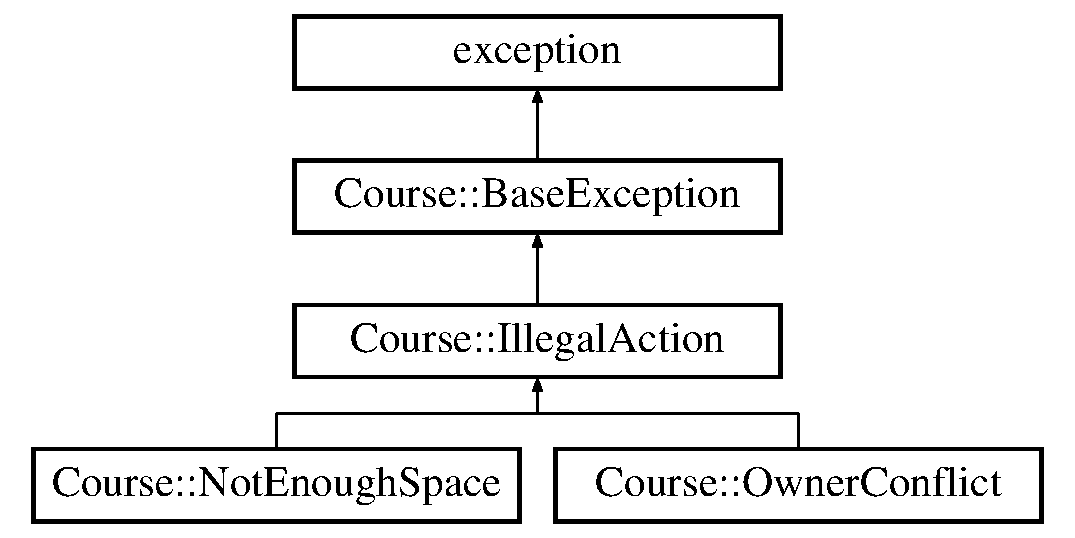
\includegraphics[height=4.000000cm]{classCourse_1_1IllegalAction}
\end{center}
\end{figure}
\subsection*{Public Member Functions}
\begin{DoxyCompactItemize}
\item 
\hyperlink{classCourse_1_1IllegalAction_aec1eb2ce3f7f9d5c96b70818d88d7514}{Illegal\-Action} (const std\-::string \&\hyperlink{classCourse_1_1BaseException_ac5a744a6af6f2ba9198b58e52bb62f5a}{msg}=\char`\"{}\char`\"{})
\begin{DoxyCompactList}\small\item\em Exception Constructor. \end{DoxyCompactList}\item 
virtual \hyperlink{classCourse_1_1IllegalAction_ae2002931f9099ea01176273cb8d6c9d3}{$\sim$\-Illegal\-Action} ()=default
\begin{DoxyCompactList}\small\item\em $\sim$\-Exception Default destructor \end{DoxyCompactList}\end{DoxyCompactItemize}


\subsection{Detailed Description}
The \hyperlink{classCourse_1_1IllegalAction}{Illegal\-Action} exception is usually used in cases, where an illegal game action was attempted. 

\subsection{Constructor \& Destructor Documentation}
\hypertarget{classCourse_1_1IllegalAction_aec1eb2ce3f7f9d5c96b70818d88d7514}{\index{Course\-::\-Illegal\-Action@{Course\-::\-Illegal\-Action}!Illegal\-Action@{Illegal\-Action}}
\index{Illegal\-Action@{Illegal\-Action}!Course::IllegalAction@{Course\-::\-Illegal\-Action}}
\subsubsection[{Illegal\-Action}]{\setlength{\rightskip}{0pt plus 5cm}Course\-::\-Illegal\-Action\-::\-Illegal\-Action (
\begin{DoxyParamCaption}
\item[{const std\-::string \&}]{msg = {\ttfamily \char`\"{}\char`\"{}}}
\end{DoxyParamCaption}
)\hspace{0.3cm}{\ttfamily [inline]}, {\ttfamily [explicit]}}}\label{classCourse_1_1IllegalAction_aec1eb2ce3f7f9d5c96b70818d88d7514}


Exception Constructor. 


\begin{DoxyParams}{Parameters}
{\em msg} & std\-::string describing the reason for exception. \\
\hline
\end{DoxyParams}
\hypertarget{classCourse_1_1IllegalAction_ae2002931f9099ea01176273cb8d6c9d3}{\index{Course\-::\-Illegal\-Action@{Course\-::\-Illegal\-Action}!$\sim$\-Illegal\-Action@{$\sim$\-Illegal\-Action}}
\index{$\sim$\-Illegal\-Action@{$\sim$\-Illegal\-Action}!Course::IllegalAction@{Course\-::\-Illegal\-Action}}
\subsubsection[{$\sim$\-Illegal\-Action}]{\setlength{\rightskip}{0pt plus 5cm}virtual Course\-::\-Illegal\-Action\-::$\sim$\-Illegal\-Action (
\begin{DoxyParamCaption}
{}
\end{DoxyParamCaption}
)\hspace{0.3cm}{\ttfamily [virtual]}, {\ttfamily [default]}}}\label{classCourse_1_1IllegalAction_ae2002931f9099ea01176273cb8d6c9d3}


$\sim$\-Exception Default destructor 



The documentation for this class was generated from the following file\-:\begin{DoxyCompactItemize}
\item 
Course/\-Course\-Lib/exceptions/\hyperlink{illegalaction_8h}{illegalaction.\-h}\end{DoxyCompactItemize}

\hypertarget{classCourse_1_1InvalidPointer}{\section{Course\-:\-:Invalid\-Pointer Class Reference}
\label{classCourse_1_1InvalidPointer}\index{Course\-::\-Invalid\-Pointer@{Course\-::\-Invalid\-Pointer}}
}


The \hyperlink{classCourse_1_1InvalidPointer}{Invalid\-Pointer} exception is usually used in cases, where data can't be accessed through a pointer.  




{\ttfamily \#include $<$invalidpointer.\-h$>$}

Inheritance diagram for Course\-:\-:Invalid\-Pointer\-:\begin{figure}[H]
\begin{center}
\leavevmode
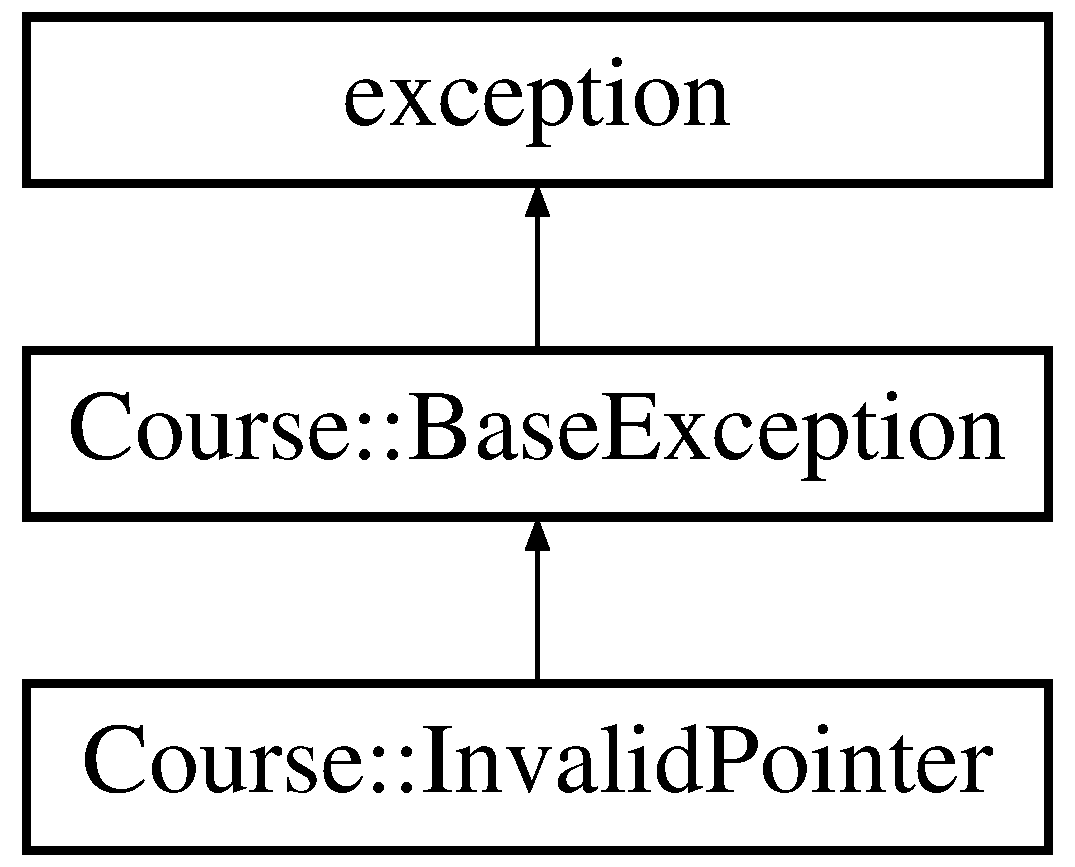
\includegraphics[height=3.000000cm]{classCourse_1_1InvalidPointer}
\end{center}
\end{figure}
\subsection*{Public Member Functions}
\begin{DoxyCompactItemize}
\item 
\hyperlink{classCourse_1_1InvalidPointer_a50e19c157520ba167d71e0c2a2ef5e08}{Invalid\-Pointer} (const std\-::string \&\hyperlink{classCourse_1_1BaseException_ac5a744a6af6f2ba9198b58e52bb62f5a}{msg}=\char`\"{}\char`\"{})
\begin{DoxyCompactList}\small\item\em Exception Constructor. \end{DoxyCompactList}\item 
virtual \hyperlink{classCourse_1_1InvalidPointer_a810f843d49a0fc64dfedddbe4a1e447e}{$\sim$\-Invalid\-Pointer} ()=default
\begin{DoxyCompactList}\small\item\em $\sim$\-Exception Default destructor \end{DoxyCompactList}\end{DoxyCompactItemize}


\subsection{Detailed Description}
The \hyperlink{classCourse_1_1InvalidPointer}{Invalid\-Pointer} exception is usually used in cases, where data can't be accessed through a pointer. 

\subsection{Constructor \& Destructor Documentation}
\hypertarget{classCourse_1_1InvalidPointer_a50e19c157520ba167d71e0c2a2ef5e08}{\index{Course\-::\-Invalid\-Pointer@{Course\-::\-Invalid\-Pointer}!Invalid\-Pointer@{Invalid\-Pointer}}
\index{Invalid\-Pointer@{Invalid\-Pointer}!Course::InvalidPointer@{Course\-::\-Invalid\-Pointer}}
\subsubsection[{Invalid\-Pointer}]{\setlength{\rightskip}{0pt plus 5cm}Course\-::\-Invalid\-Pointer\-::\-Invalid\-Pointer (
\begin{DoxyParamCaption}
\item[{const std\-::string \&}]{msg = {\ttfamily \char`\"{}\char`\"{}}}
\end{DoxyParamCaption}
)\hspace{0.3cm}{\ttfamily [inline]}, {\ttfamily [explicit]}}}\label{classCourse_1_1InvalidPointer_a50e19c157520ba167d71e0c2a2ef5e08}


Exception Constructor. 


\begin{DoxyParams}{Parameters}
{\em msg} & std\-::string describing the reason for exception. \\
\hline
\end{DoxyParams}
\hypertarget{classCourse_1_1InvalidPointer_a810f843d49a0fc64dfedddbe4a1e447e}{\index{Course\-::\-Invalid\-Pointer@{Course\-::\-Invalid\-Pointer}!$\sim$\-Invalid\-Pointer@{$\sim$\-Invalid\-Pointer}}
\index{$\sim$\-Invalid\-Pointer@{$\sim$\-Invalid\-Pointer}!Course::InvalidPointer@{Course\-::\-Invalid\-Pointer}}
\subsubsection[{$\sim$\-Invalid\-Pointer}]{\setlength{\rightskip}{0pt plus 5cm}virtual Course\-::\-Invalid\-Pointer\-::$\sim$\-Invalid\-Pointer (
\begin{DoxyParamCaption}
{}
\end{DoxyParamCaption}
)\hspace{0.3cm}{\ttfamily [virtual]}, {\ttfamily [default]}}}\label{classCourse_1_1InvalidPointer_a810f843d49a0fc64dfedddbe4a1e447e}


$\sim$\-Exception Default destructor 



The documentation for this class was generated from the following file\-:\begin{DoxyCompactItemize}
\item 
Course/\-Course\-Lib/exceptions/\hyperlink{invalidpointer_8h}{invalidpointer.\-h}\end{DoxyCompactItemize}

\hypertarget{classCourse_1_1iObjectManager}{\section{Course\-:\-:i\-Object\-Manager Class Reference}
\label{classCourse_1_1iObjectManager}\index{Course\-::i\-Object\-Manager@{Course\-::i\-Object\-Manager}}
}


The \hyperlink{classCourse_1_1iObjectManager}{i\-Object\-Manager} class is an interface which the Course-\/side code uses to interact with the Object\-Manager implemented by the students.  




{\ttfamily \#include $<$iobjectmanager.\-h$>$}

Inheritance diagram for Course\-:\-:i\-Object\-Manager\-:\begin{figure}[H]
\begin{center}
\leavevmode
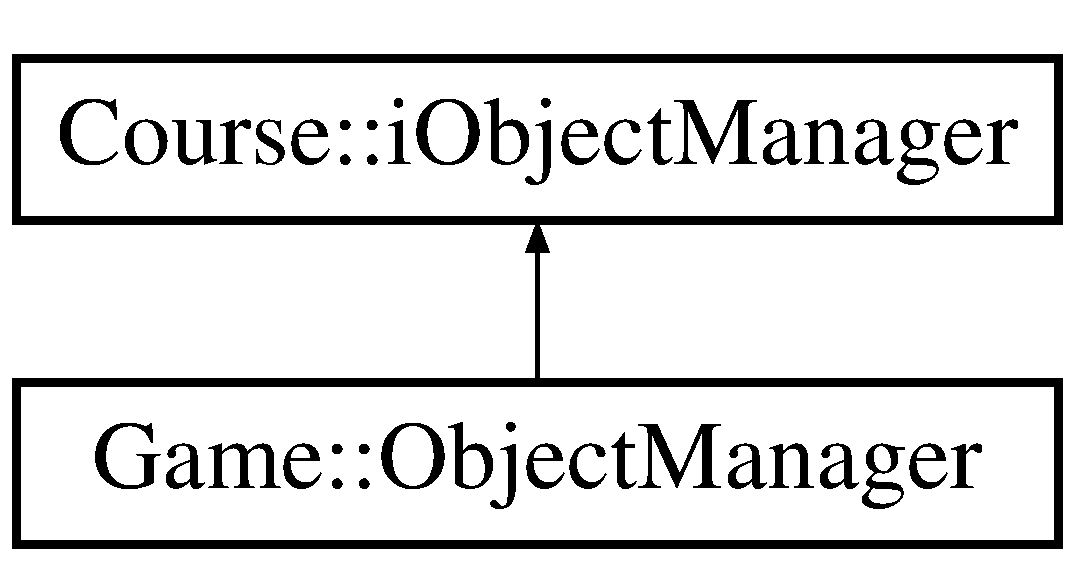
\includegraphics[height=2.000000cm]{classCourse_1_1iObjectManager}
\end{center}
\end{figure}
\subsection*{Public Member Functions}
\begin{DoxyCompactItemize}
\item 
virtual \hyperlink{classCourse_1_1iObjectManager_afe7f4ca78e8bcb3d94f92cbcb3e36a6f}{$\sim$i\-Object\-Manager} ()=default
\begin{DoxyCompactList}\small\item\em Default destructor. \end{DoxyCompactList}\item 
virtual void \hyperlink{classCourse_1_1iObjectManager_a826fa55229bdc23c49f847245fbdda95}{add\-Tiles} (const std\-::vector$<$ std\-::shared\-\_\-ptr$<$ \hyperlink{classCourse_1_1TileBase}{Tile\-Base} $>$$>$ \&tiles)=0
\begin{DoxyCompactList}\small\item\em Adds new tiles to the Object\-Manager. \end{DoxyCompactList}\item 
virtual std\-::shared\-\_\-ptr$<$ \hyperlink{classCourse_1_1TileBase}{Tile\-Base} $>$ \hyperlink{classCourse_1_1iObjectManager_afd7ab74d8a4cfedd50340c1e9096672d}{get\-Tile} (const \hyperlink{classCourse_1_1Coordinate}{Coordinate} \&coordinate)=0
\begin{DoxyCompactList}\small\item\em Returns a shared pointer to a Tile that has specified coordinate. \end{DoxyCompactList}\item 
virtual std\-::shared\-\_\-ptr$<$ \hyperlink{classCourse_1_1TileBase}{Tile\-Base} $>$ \hyperlink{classCourse_1_1iObjectManager_a7c3280cc01c8cf77d49afe88ca0e6b48}{get\-Tile} (const \hyperlink{namespaceCourse_a9a16e743c9813da00109e4991afd2f3e}{Object\-Id} \&id)=0
\begin{DoxyCompactList}\small\item\em Returns a shared pointer to a Tile that has specified I\-D. \end{DoxyCompactList}\item 
virtual std\-::vector\\*
$<$ std\-::shared\-\_\-ptr$<$ \hyperlink{classCourse_1_1TileBase}{Tile\-Base} $>$ $>$ \hyperlink{classCourse_1_1iObjectManager_ac1b0d805db508f80477fbb7e5987e4e4}{get\-Tiles} (const std\-::vector$<$ \hyperlink{classCourse_1_1Coordinate}{Coordinate} $>$ \&coordinates)=0
\begin{DoxyCompactList}\small\item\em Returns a vector of shared pointers to Tiles specified by a vector of Coordinates. \end{DoxyCompactList}\end{DoxyCompactItemize}


\subsection{Detailed Description}
The \hyperlink{classCourse_1_1iObjectManager}{i\-Object\-Manager} class is an interface which the Course-\/side code uses to interact with the Object\-Manager implemented by the students. 

\begin{DoxyNote}{Note}
The interface declares only functions required by the Course-\/side code. The actual implementation can (and should!) contain more stuff. 
\end{DoxyNote}


\subsection{Constructor \& Destructor Documentation}
\hypertarget{classCourse_1_1iObjectManager_afe7f4ca78e8bcb3d94f92cbcb3e36a6f}{\index{Course\-::i\-Object\-Manager@{Course\-::i\-Object\-Manager}!$\sim$i\-Object\-Manager@{$\sim$i\-Object\-Manager}}
\index{$\sim$i\-Object\-Manager@{$\sim$i\-Object\-Manager}!Course::iObjectManager@{Course\-::i\-Object\-Manager}}
\subsubsection[{$\sim$i\-Object\-Manager}]{\setlength{\rightskip}{0pt plus 5cm}virtual Course\-::i\-Object\-Manager\-::$\sim$i\-Object\-Manager (
\begin{DoxyParamCaption}
{}
\end{DoxyParamCaption}
)\hspace{0.3cm}{\ttfamily [virtual]}, {\ttfamily [default]}}}\label{classCourse_1_1iObjectManager_afe7f4ca78e8bcb3d94f92cbcb3e36a6f}


Default destructor. 



\subsection{Member Function Documentation}
\hypertarget{classCourse_1_1iObjectManager_a826fa55229bdc23c49f847245fbdda95}{\index{Course\-::i\-Object\-Manager@{Course\-::i\-Object\-Manager}!add\-Tiles@{add\-Tiles}}
\index{add\-Tiles@{add\-Tiles}!Course::iObjectManager@{Course\-::i\-Object\-Manager}}
\subsubsection[{add\-Tiles}]{\setlength{\rightskip}{0pt plus 5cm}virtual void Course\-::i\-Object\-Manager\-::add\-Tiles (
\begin{DoxyParamCaption}
\item[{const std\-::vector$<$ std\-::shared\-\_\-ptr$<$ {\bf Tile\-Base} $>$$>$ \&}]{tiles}
\end{DoxyParamCaption}
)\hspace{0.3cm}{\ttfamily [pure virtual]}}}\label{classCourse_1_1iObjectManager_a826fa55229bdc23c49f847245fbdda95}


Adds new tiles to the Object\-Manager. 


\begin{DoxyParams}{Parameters}
{\em tiles} & a vector that contains the Tiles to be added. \\
\hline
\end{DoxyParams}
\begin{DoxyPostcond}{Postcondition}
The tile-\/pointers in the vector are stored in the Object\-Manager. Exception Guarantee\-: Basic 
\end{DoxyPostcond}


Implemented in \hyperlink{classGame_1_1ObjectManager_a92fb3bc8bebd8d08bf080ead20cfff10}{Game\-::\-Object\-Manager}.

\hypertarget{classCourse_1_1iObjectManager_afd7ab74d8a4cfedd50340c1e9096672d}{\index{Course\-::i\-Object\-Manager@{Course\-::i\-Object\-Manager}!get\-Tile@{get\-Tile}}
\index{get\-Tile@{get\-Tile}!Course::iObjectManager@{Course\-::i\-Object\-Manager}}
\subsubsection[{get\-Tile}]{\setlength{\rightskip}{0pt plus 5cm}virtual std\-::shared\-\_\-ptr$<${\bf Tile\-Base}$>$ Course\-::i\-Object\-Manager\-::get\-Tile (
\begin{DoxyParamCaption}
\item[{const {\bf Coordinate} \&}]{coordinate}
\end{DoxyParamCaption}
)\hspace{0.3cm}{\ttfamily [pure virtual]}}}\label{classCourse_1_1iObjectManager_afd7ab74d8a4cfedd50340c1e9096672d}


Returns a shared pointer to a Tile that has specified coordinate. 


\begin{DoxyParams}{Parameters}
{\em coordinate} & Requested Tile's \hyperlink{classCourse_1_1Coordinate}{Coordinate} \\
\hline
\end{DoxyParams}
\begin{DoxyReturn}{Returns}
a pointer to a Tile that has the given coordinate. If no for the coordinate exists, return empty pointer. 
\end{DoxyReturn}
\begin{DoxyPostcond}{Postcondition}
Exception Guarantee\-: Basic 
\end{DoxyPostcond}


Implemented in \hyperlink{classGame_1_1ObjectManager_a0d1b58925d8baca124f611a697ea987c}{Game\-::\-Object\-Manager}.

\hypertarget{classCourse_1_1iObjectManager_a7c3280cc01c8cf77d49afe88ca0e6b48}{\index{Course\-::i\-Object\-Manager@{Course\-::i\-Object\-Manager}!get\-Tile@{get\-Tile}}
\index{get\-Tile@{get\-Tile}!Course::iObjectManager@{Course\-::i\-Object\-Manager}}
\subsubsection[{get\-Tile}]{\setlength{\rightskip}{0pt plus 5cm}virtual std\-::shared\-\_\-ptr$<${\bf Tile\-Base}$>$ Course\-::i\-Object\-Manager\-::get\-Tile (
\begin{DoxyParamCaption}
\item[{const {\bf Object\-Id} \&}]{id}
\end{DoxyParamCaption}
)\hspace{0.3cm}{\ttfamily [pure virtual]}}}\label{classCourse_1_1iObjectManager_a7c3280cc01c8cf77d49afe88ca0e6b48}


Returns a shared pointer to a Tile that has specified I\-D. 


\begin{DoxyParams}{Parameters}
{\em id} & Tile's Object\-Id. \\
\hline
\end{DoxyParams}
\begin{DoxyReturn}{Returns}
a pointer to the Tile that has the given I\-D If no for the id exists, return empty pointer. 
\end{DoxyReturn}
\begin{DoxyPostcond}{Postcondition}
Exception Guarantee\-: Basic 
\end{DoxyPostcond}


Implemented in \hyperlink{classGame_1_1ObjectManager_a299c9708f9e405d78a10b0aa7d1658aa}{Game\-::\-Object\-Manager}.

\hypertarget{classCourse_1_1iObjectManager_ac1b0d805db508f80477fbb7e5987e4e4}{\index{Course\-::i\-Object\-Manager@{Course\-::i\-Object\-Manager}!get\-Tiles@{get\-Tiles}}
\index{get\-Tiles@{get\-Tiles}!Course::iObjectManager@{Course\-::i\-Object\-Manager}}
\subsubsection[{get\-Tiles}]{\setlength{\rightskip}{0pt plus 5cm}virtual std\-::vector$<$std\-::shared\-\_\-ptr$<${\bf Tile\-Base}$>$ $>$ Course\-::i\-Object\-Manager\-::get\-Tiles (
\begin{DoxyParamCaption}
\item[{const std\-::vector$<$ {\bf Coordinate} $>$ \&}]{coordinates}
\end{DoxyParamCaption}
)\hspace{0.3cm}{\ttfamily [pure virtual]}}}\label{classCourse_1_1iObjectManager_ac1b0d805db508f80477fbb7e5987e4e4}


Returns a vector of shared pointers to Tiles specified by a vector of Coordinates. 


\begin{DoxyParams}{Parameters}
{\em coordinates} & a vector of Coordinates for the requested Tiles \\
\hline
\end{DoxyParams}
\begin{DoxyReturn}{Returns}
Vector of that contains pointers to Tile's that match the coordinates. The vector is empty if no matches were made. 
\end{DoxyReturn}
\begin{DoxyPostcond}{Postcondition}
Exception Guarantee\-: Basic 
\end{DoxyPostcond}


Implemented in \hyperlink{classGame_1_1ObjectManager_ad4646477bd85b931f028a1a8f5916f3e}{Game\-::\-Object\-Manager}.



The documentation for this class was generated from the following file\-:\begin{DoxyCompactItemize}
\item 
Course/\-Course\-Lib/interfaces/\hyperlink{iobjectmanager_8h}{iobjectmanager.\-h}\end{DoxyCompactItemize}

\hypertarget{classCourse_1_1KeyError}{\section{Course\-:\-:Key\-Error Class Reference}
\label{classCourse_1_1KeyError}\index{Course\-::\-Key\-Error@{Course\-::\-Key\-Error}}
}


The \hyperlink{classCourse_1_1KeyError}{Key\-Error} class is an Exception-\/class for cases where the used key is invalid.  




{\ttfamily \#include $<$keyerror.\-h$>$}

Inheritance diagram for Course\-:\-:Key\-Error\-:\begin{figure}[H]
\begin{center}
\leavevmode
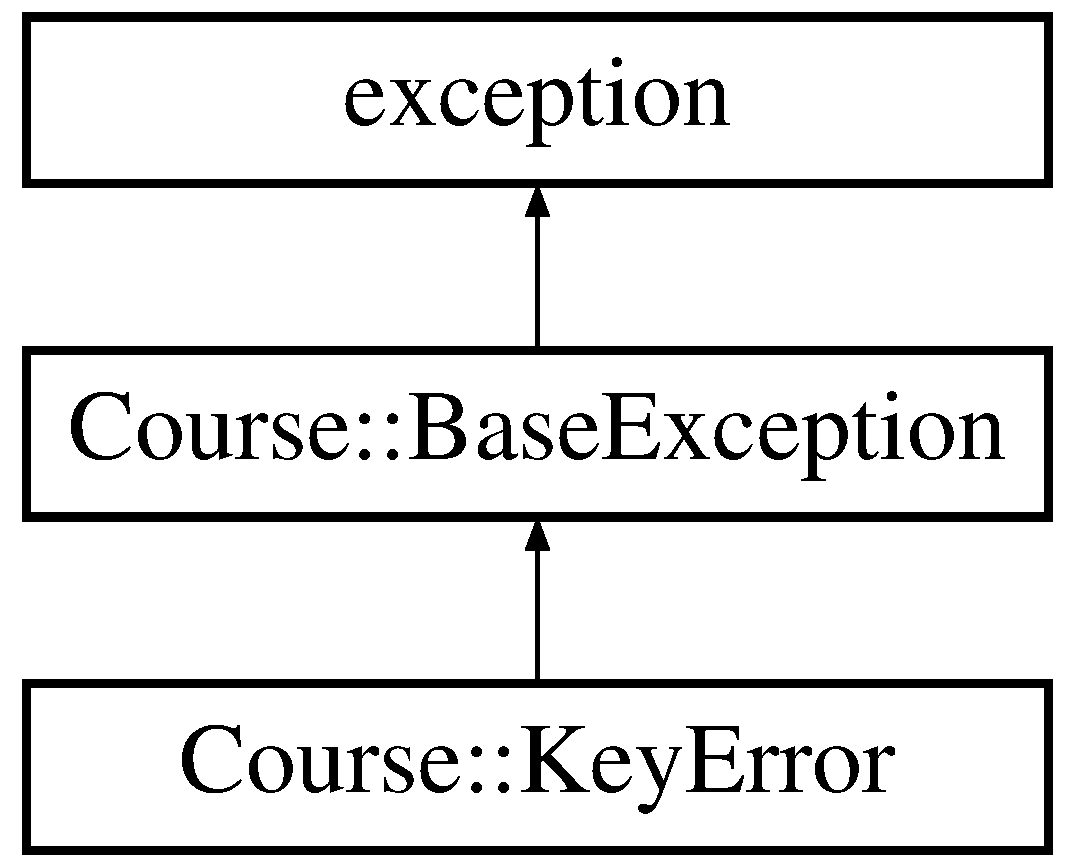
\includegraphics[height=3.000000cm]{classCourse_1_1KeyError}
\end{center}
\end{figure}
\subsection*{Public Member Functions}
\begin{DoxyCompactItemize}
\item 
\hyperlink{classCourse_1_1KeyError_a99407655a8d0d86cb3d7daf6765a601c}{Key\-Error} (const std\-::string \&\hyperlink{classCourse_1_1BaseException_ac5a744a6af6f2ba9198b58e52bb62f5a}{msg}=\char`\"{}\char`\"{})
\begin{DoxyCompactList}\small\item\em Exception Constructor. \end{DoxyCompactList}\item 
virtual \hyperlink{classCourse_1_1KeyError_a48b0429d954fd992dc29f44437ae056c}{$\sim$\-Key\-Error} ()=default
\begin{DoxyCompactList}\small\item\em $\sim$\-Exception Default destructor \end{DoxyCompactList}\end{DoxyCompactItemize}


\subsection{Detailed Description}
The \hyperlink{classCourse_1_1KeyError}{Key\-Error} class is an Exception-\/class for cases where the used key is invalid. 

\subsection{Constructor \& Destructor Documentation}
\hypertarget{classCourse_1_1KeyError_a99407655a8d0d86cb3d7daf6765a601c}{\index{Course\-::\-Key\-Error@{Course\-::\-Key\-Error}!Key\-Error@{Key\-Error}}
\index{Key\-Error@{Key\-Error}!Course::KeyError@{Course\-::\-Key\-Error}}
\subsubsection[{Key\-Error}]{\setlength{\rightskip}{0pt plus 5cm}Course\-::\-Key\-Error\-::\-Key\-Error (
\begin{DoxyParamCaption}
\item[{const std\-::string \&}]{msg = {\ttfamily \char`\"{}\char`\"{}}}
\end{DoxyParamCaption}
)\hspace{0.3cm}{\ttfamily [inline]}, {\ttfamily [explicit]}}}\label{classCourse_1_1KeyError_a99407655a8d0d86cb3d7daf6765a601c}


Exception Constructor. 


\begin{DoxyParams}{Parameters}
{\em msg} & std\-::string describing the reason for exception. \\
\hline
\end{DoxyParams}
\hypertarget{classCourse_1_1KeyError_a48b0429d954fd992dc29f44437ae056c}{\index{Course\-::\-Key\-Error@{Course\-::\-Key\-Error}!$\sim$\-Key\-Error@{$\sim$\-Key\-Error}}
\index{$\sim$\-Key\-Error@{$\sim$\-Key\-Error}!Course::KeyError@{Course\-::\-Key\-Error}}
\subsubsection[{$\sim$\-Key\-Error}]{\setlength{\rightskip}{0pt plus 5cm}virtual Course\-::\-Key\-Error\-::$\sim$\-Key\-Error (
\begin{DoxyParamCaption}
{}
\end{DoxyParamCaption}
)\hspace{0.3cm}{\ttfamily [virtual]}, {\ttfamily [default]}}}\label{classCourse_1_1KeyError_a48b0429d954fd992dc29f44437ae056c}


$\sim$\-Exception Default destructor 



The documentation for this class was generated from the following file\-:\begin{DoxyCompactItemize}
\item 
Course/\-Course\-Lib/exceptions/\hyperlink{keyerror_8h}{keyerror.\-h}\end{DoxyCompactItemize}

\hypertarget{classGame_1_1MapItem}{\section{Game\-:\-:Map\-Item Class Reference}
\label{classGame_1_1MapItem}\index{Game\-::\-Map\-Item@{Game\-::\-Map\-Item}}
}


The \hyperlink{classGame_1_1MapItem}{Map\-Item} class is a custom Q\-Graphics\-Item that acts as a single Game\-Object's graphical element.  




{\ttfamily \#include $<$mapitem.\-h$>$}

Inheritance diagram for Game\-:\-:Map\-Item\-:\begin{figure}[H]
\begin{center}
\leavevmode
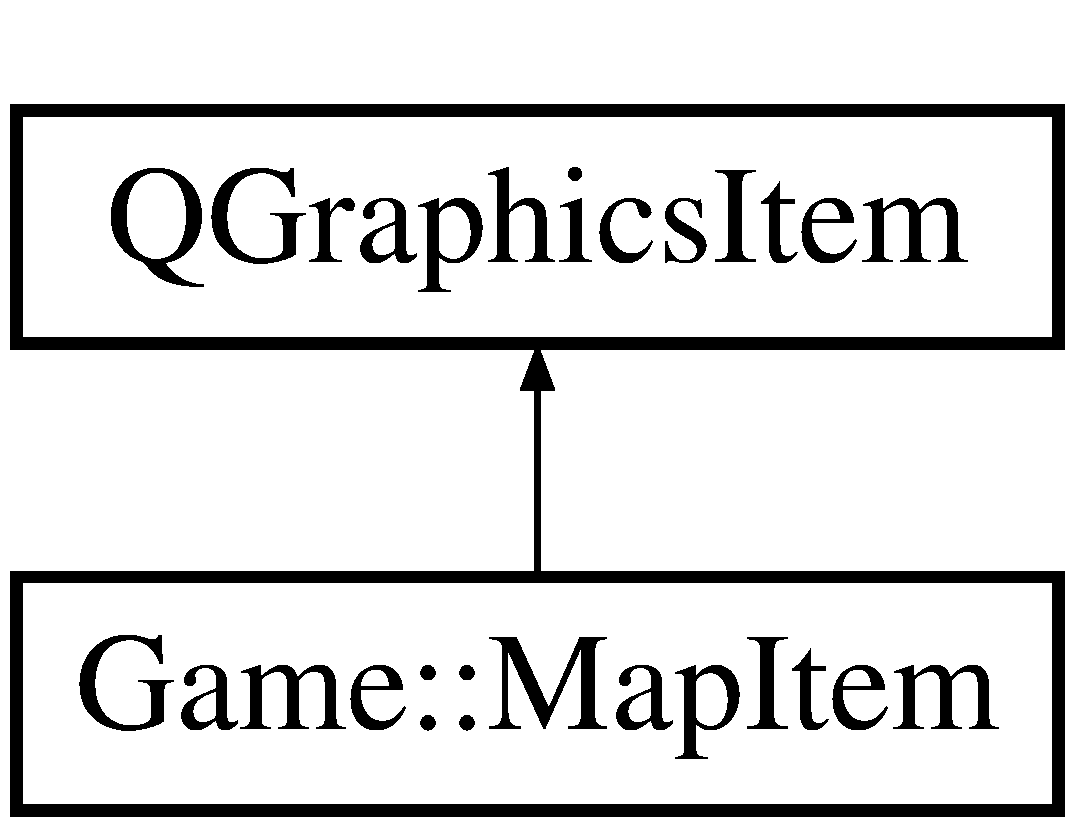
\includegraphics[height=2.000000cm]{classGame_1_1MapItem}
\end{center}
\end{figure}
\subsection*{Public Member Functions}
\begin{DoxyCompactItemize}
\item 
\hyperlink{classGame_1_1MapItem_adab3634fb773e7b185b08b9914bb93e7}{Map\-Item} (const std\-::shared\-\_\-ptr$<$ \hyperlink{classCourse_1_1GameObject}{Course\-::\-Game\-Object} $>$ \&obj, int size, int offset)
\begin{DoxyCompactList}\small\item\em Constructor. \end{DoxyCompactList}\item 
Q\-Rect\-F \hyperlink{classGame_1_1MapItem_a564c803217c15efdd414bc47bc385d94}{bounding\-Rect} () const override
\begin{DoxyCompactList}\small\item\em bounding\-Rect \end{DoxyCompactList}\item 
Q\-Pixmap \hyperlink{classGame_1_1MapItem_a1cbdeaa3793d5c9ba65d792ca44cfad2}{image} () const 
\begin{DoxyCompactList}\small\item\em Finds the corresponding image for the object. \end{DoxyCompactList}\item 
void \hyperlink{classGame_1_1MapItem_a8e18b37b2f48bf586b650dd97bfd03e4}{paint} (Q\-Painter $\ast$painter, const Q\-Style\-Option\-Graphics\-Item $\ast$option, Q\-Widget $\ast$widget)
\begin{DoxyCompactList}\small\item\em paints the item \end{DoxyCompactList}\item 
const std\-::shared\-\_\-ptr\\*
$<$ \hyperlink{classCourse_1_1GameObject}{Course\-::\-Game\-Object} $>$ \& \hyperlink{classGame_1_1MapItem_aa61f3c3867a3805669210c259b2f573e}{get\-Bound\-Object} ()
\begin{DoxyCompactList}\small\item\em get\-Bound\-Object \end{DoxyCompactList}\item 
void \hyperlink{classGame_1_1MapItem_a5bd976eefca99e0ff2f8767d7f1c5c03}{update\-Loc} ()
\begin{DoxyCompactList}\small\item\em update\-Loc moves the item if the position has changed. \end{DoxyCompactList}\item 
bool \hyperlink{classGame_1_1MapItem_a1183a2283108cead408f52d36e53a41b}{is\-Same\-Obj} (std\-::shared\-\_\-ptr$<$ \hyperlink{classCourse_1_1GameObject}{Course\-::\-Game\-Object} $>$ obj)
\begin{DoxyCompactList}\small\item\em checks if this instance has obj as bound obj. \end{DoxyCompactList}\end{DoxyCompactItemize}
\subsection*{Private Attributes}
\begin{DoxyCompactItemize}
\item 
const std\-::shared\-\_\-ptr\\*
$<$ \hyperlink{classCourse_1_1GameObject}{Course\-::\-Game\-Object} $>$ \hyperlink{classGame_1_1MapItem_a501cc900c7d06991d795f9148650b070}{m\-\_\-gameobject}
\item 
Q\-Point \hyperlink{classGame_1_1MapItem_a0f9e884f907244ada7432215fe01b2cd}{m\-\_\-scenelocation}
\item 
int \hyperlink{classGame_1_1MapItem_a7550fe4dec9a0b7d7f42e0d1f25c0813}{m\-\_\-size}
\item 
int \hyperlink{classGame_1_1MapItem_a4d704ac5bfc0a70926d8dfc51219e2cd}{m\-\_\-offset}
\end{DoxyCompactItemize}
\subsection*{Static Private Attributes}
\begin{DoxyCompactItemize}
\item 
static \hyperlink{namespaceGame_a1fe13161652a186ddb92a1774eeb6eaa}{Color\-Map} \hyperlink{classGame_1_1MapItem_a2e9e5bfec64df70790559d7c2fe374b0}{c\-\_\-mapcolors} = \{\}
\end{DoxyCompactItemize}


\subsection{Detailed Description}
The \hyperlink{classGame_1_1MapItem}{Map\-Item} class is a custom Q\-Graphics\-Item that acts as a single Game\-Object's graphical element. 

\subsection{Constructor \& Destructor Documentation}
\hypertarget{classGame_1_1MapItem_adab3634fb773e7b185b08b9914bb93e7}{\index{Game\-::\-Map\-Item@{Game\-::\-Map\-Item}!Map\-Item@{Map\-Item}}
\index{Map\-Item@{Map\-Item}!Game::MapItem@{Game\-::\-Map\-Item}}
\subsubsection[{Map\-Item}]{\setlength{\rightskip}{0pt plus 5cm}Game\-::\-Map\-Item\-::\-Map\-Item (
\begin{DoxyParamCaption}
\item[{const std\-::shared\-\_\-ptr$<$ {\bf Course\-::\-Game\-Object} $>$ \&}]{obj, }
\item[{int}]{size, }
\item[{int}]{offset}
\end{DoxyParamCaption}
)}}\label{classGame_1_1MapItem_adab3634fb773e7b185b08b9914bb93e7}


Constructor. 


\begin{DoxyParams}{Parameters}
{\em obj} & shared\-\_\-ptr to the obj. \\
\hline
{\em size} & of the created item in pixels. \\
\hline
{\em offset} & for the item in the tile \\
\hline
\end{DoxyParams}
\begin{DoxyPrecond}{Precondition}
obj must have a valid Coordinate. 
\end{DoxyPrecond}


\subsection{Member Function Documentation}
\hypertarget{classGame_1_1MapItem_a564c803217c15efdd414bc47bc385d94}{\index{Game\-::\-Map\-Item@{Game\-::\-Map\-Item}!bounding\-Rect@{bounding\-Rect}}
\index{bounding\-Rect@{bounding\-Rect}!Game::MapItem@{Game\-::\-Map\-Item}}
\subsubsection[{bounding\-Rect}]{\setlength{\rightskip}{0pt plus 5cm}Q\-Rect\-F Game\-::\-Map\-Item\-::bounding\-Rect (
\begin{DoxyParamCaption}
{}
\end{DoxyParamCaption}
) const\hspace{0.3cm}{\ttfamily [override]}}}\label{classGame_1_1MapItem_a564c803217c15efdd414bc47bc385d94}


bounding\-Rect 

\begin{DoxyReturn}{Returns}
the bounding rectangle of this item. 
\end{DoxyReturn}
\hypertarget{classGame_1_1MapItem_aa61f3c3867a3805669210c259b2f573e}{\index{Game\-::\-Map\-Item@{Game\-::\-Map\-Item}!get\-Bound\-Object@{get\-Bound\-Object}}
\index{get\-Bound\-Object@{get\-Bound\-Object}!Game::MapItem@{Game\-::\-Map\-Item}}
\subsubsection[{get\-Bound\-Object}]{\setlength{\rightskip}{0pt plus 5cm}const std\-::shared\-\_\-ptr$<$ {\bf Course\-::\-Game\-Object} $>$ \& Game\-::\-Map\-Item\-::get\-Bound\-Object (
\begin{DoxyParamCaption}
{}
\end{DoxyParamCaption}
)}}\label{classGame_1_1MapItem_aa61f3c3867a3805669210c259b2f573e}


get\-Bound\-Object 

\begin{DoxyReturn}{Returns}
the object this item is bound to. 
\end{DoxyReturn}
\hypertarget{classGame_1_1MapItem_a1cbdeaa3793d5c9ba65d792ca44cfad2}{\index{Game\-::\-Map\-Item@{Game\-::\-Map\-Item}!image@{image}}
\index{image@{image}!Game::MapItem@{Game\-::\-Map\-Item}}
\subsubsection[{image}]{\setlength{\rightskip}{0pt plus 5cm}Q\-Pixmap Game\-::\-Map\-Item\-::image (
\begin{DoxyParamCaption}
{}
\end{DoxyParamCaption}
) const}}\label{classGame_1_1MapItem_a1cbdeaa3793d5c9ba65d792ca44cfad2}


Finds the corresponding image for the object. 

\begin{DoxyPrecond}{Precondition}
object must have an image named accordingly to its object type 
\end{DoxyPrecond}
\begin{DoxyReturn}{Returns}
object's image 
\end{DoxyReturn}
\begin{DoxyPostcond}{Postcondition}
Exception guarantee\-: No-\/throw 
\end{DoxyPostcond}
\hypertarget{classGame_1_1MapItem_a1183a2283108cead408f52d36e53a41b}{\index{Game\-::\-Map\-Item@{Game\-::\-Map\-Item}!is\-Same\-Obj@{is\-Same\-Obj}}
\index{is\-Same\-Obj@{is\-Same\-Obj}!Game::MapItem@{Game\-::\-Map\-Item}}
\subsubsection[{is\-Same\-Obj}]{\setlength{\rightskip}{0pt plus 5cm}bool Game\-::\-Map\-Item\-::is\-Same\-Obj (
\begin{DoxyParamCaption}
\item[{std\-::shared\-\_\-ptr$<$ {\bf Course\-::\-Game\-Object} $>$}]{obj}
\end{DoxyParamCaption}
)}}\label{classGame_1_1MapItem_a1183a2283108cead408f52d36e53a41b}


checks if this instance has obj as bound obj. 


\begin{DoxyParams}{Parameters}
{\em obj} & to compare to. \\
\hline
\end{DoxyParams}
\begin{DoxyReturn}{Returns}
True\-: if obj is pointing to the same object as this item. False otherwise. 
\end{DoxyReturn}
\hypertarget{classGame_1_1MapItem_a8e18b37b2f48bf586b650dd97bfd03e4}{\index{Game\-::\-Map\-Item@{Game\-::\-Map\-Item}!paint@{paint}}
\index{paint@{paint}!Game::MapItem@{Game\-::\-Map\-Item}}
\subsubsection[{paint}]{\setlength{\rightskip}{0pt plus 5cm}void Game\-::\-Map\-Item\-::paint (
\begin{DoxyParamCaption}
\item[{Q\-Painter $\ast$}]{painter, }
\item[{const Q\-Style\-Option\-Graphics\-Item $\ast$}]{option, }
\item[{Q\-Widget $\ast$}]{widget}
\end{DoxyParamCaption}
)}}\label{classGame_1_1MapItem_a8e18b37b2f48bf586b650dd97bfd03e4}


paints the item 


\begin{DoxyParams}{Parameters}
{\em painter} & \\
\hline
{\em option} & \\
\hline
{\em widget} & \\
\hline
\end{DoxyParams}
\begin{DoxyNote}{Note}
The Graphics\-View containing the scene this belongs to usually calls this function. 
\end{DoxyNote}
\hypertarget{classGame_1_1MapItem_a5bd976eefca99e0ff2f8767d7f1c5c03}{\index{Game\-::\-Map\-Item@{Game\-::\-Map\-Item}!update\-Loc@{update\-Loc}}
\index{update\-Loc@{update\-Loc}!Game::MapItem@{Game\-::\-Map\-Item}}
\subsubsection[{update\-Loc}]{\setlength{\rightskip}{0pt plus 5cm}void Game\-::\-Map\-Item\-::update\-Loc (
\begin{DoxyParamCaption}
{}
\end{DoxyParamCaption}
)}}\label{classGame_1_1MapItem_a5bd976eefca99e0ff2f8767d7f1c5c03}


update\-Loc moves the item if the position has changed. 



\subsection{Member Data Documentation}
\hypertarget{classGame_1_1MapItem_a2e9e5bfec64df70790559d7c2fe374b0}{\index{Game\-::\-Map\-Item@{Game\-::\-Map\-Item}!c\-\_\-mapcolors@{c\-\_\-mapcolors}}
\index{c\-\_\-mapcolors@{c\-\_\-mapcolors}!Game::MapItem@{Game\-::\-Map\-Item}}
\subsubsection[{c\-\_\-mapcolors}]{\setlength{\rightskip}{0pt plus 5cm}std\-::map$<$ std\-::string, Q\-Color $>$ Game\-::\-Map\-Item\-::c\-\_\-mapcolors = \{\}\hspace{0.3cm}{\ttfamily [static]}, {\ttfamily [private]}}}\label{classGame_1_1MapItem_a2e9e5bfec64df70790559d7c2fe374b0}
\hypertarget{classGame_1_1MapItem_a501cc900c7d06991d795f9148650b070}{\index{Game\-::\-Map\-Item@{Game\-::\-Map\-Item}!m\-\_\-gameobject@{m\-\_\-gameobject}}
\index{m\-\_\-gameobject@{m\-\_\-gameobject}!Game::MapItem@{Game\-::\-Map\-Item}}
\subsubsection[{m\-\_\-gameobject}]{\setlength{\rightskip}{0pt plus 5cm}const std\-::shared\-\_\-ptr$<${\bf Course\-::\-Game\-Object}$>$ Game\-::\-Map\-Item\-::m\-\_\-gameobject\hspace{0.3cm}{\ttfamily [private]}}}\label{classGame_1_1MapItem_a501cc900c7d06991d795f9148650b070}
\hypertarget{classGame_1_1MapItem_a4d704ac5bfc0a70926d8dfc51219e2cd}{\index{Game\-::\-Map\-Item@{Game\-::\-Map\-Item}!m\-\_\-offset@{m\-\_\-offset}}
\index{m\-\_\-offset@{m\-\_\-offset}!Game::MapItem@{Game\-::\-Map\-Item}}
\subsubsection[{m\-\_\-offset}]{\setlength{\rightskip}{0pt plus 5cm}int Game\-::\-Map\-Item\-::m\-\_\-offset\hspace{0.3cm}{\ttfamily [private]}}}\label{classGame_1_1MapItem_a4d704ac5bfc0a70926d8dfc51219e2cd}
\hypertarget{classGame_1_1MapItem_a0f9e884f907244ada7432215fe01b2cd}{\index{Game\-::\-Map\-Item@{Game\-::\-Map\-Item}!m\-\_\-scenelocation@{m\-\_\-scenelocation}}
\index{m\-\_\-scenelocation@{m\-\_\-scenelocation}!Game::MapItem@{Game\-::\-Map\-Item}}
\subsubsection[{m\-\_\-scenelocation}]{\setlength{\rightskip}{0pt plus 5cm}Q\-Point Game\-::\-Map\-Item\-::m\-\_\-scenelocation\hspace{0.3cm}{\ttfamily [private]}}}\label{classGame_1_1MapItem_a0f9e884f907244ada7432215fe01b2cd}
\hypertarget{classGame_1_1MapItem_a7550fe4dec9a0b7d7f42e0d1f25c0813}{\index{Game\-::\-Map\-Item@{Game\-::\-Map\-Item}!m\-\_\-size@{m\-\_\-size}}
\index{m\-\_\-size@{m\-\_\-size}!Game::MapItem@{Game\-::\-Map\-Item}}
\subsubsection[{m\-\_\-size}]{\setlength{\rightskip}{0pt plus 5cm}int Game\-::\-Map\-Item\-::m\-\_\-size\hspace{0.3cm}{\ttfamily [private]}}}\label{classGame_1_1MapItem_a7550fe4dec9a0b7d7f42e0d1f25c0813}


The documentation for this class was generated from the following files\-:\begin{DoxyCompactItemize}
\item 
Game/graphics/\hyperlink{mapitem_8h}{mapitem.\-h}\item 
Game/graphics/\hyperlink{mapitem_8cpp}{mapitem.\-cpp}\end{DoxyCompactItemize}

\hypertarget{classMapWindow}{\section{Map\-Window Class Reference}
\label{classMapWindow}\index{Map\-Window@{Map\-Window}}
}


The \hyperlink{classMapWindow}{Map\-Window} class is the main game window.  




{\ttfamily \#include $<$mapwindow.\-hh$>$}

Inheritance diagram for Map\-Window\-:\begin{figure}[H]
\begin{center}
\leavevmode
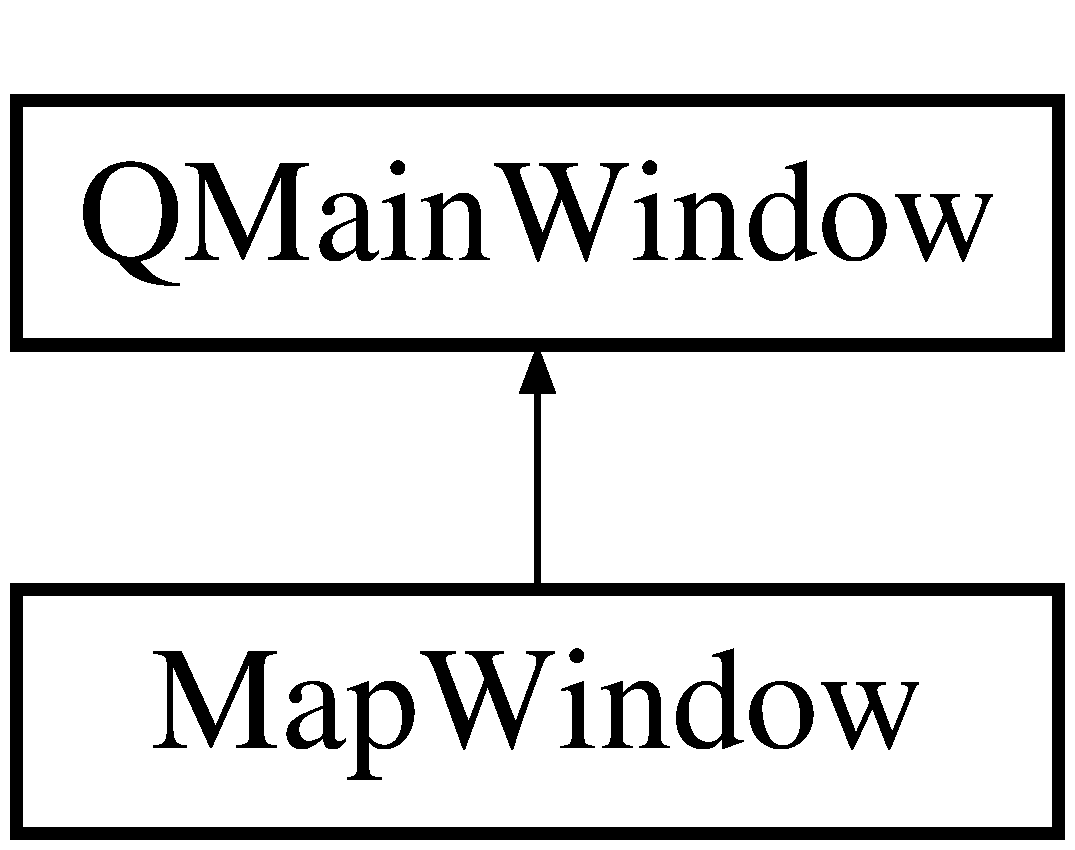
\includegraphics[height=2.000000cm]{classMapWindow}
\end{center}
\end{figure}
\subsection*{Public Slots}
\begin{DoxyCompactItemize}
\item 
void \hyperlink{classMapWindow_a39948451de86944d283ac9fc972cf271}{place\-Object} (Course\-::\-Object\-Id tile\-I\-D)
\begin{DoxyCompactList}\small\item\em Sets a Placeable\-Game\-Object onto a tile and sets \par
owners for required objects. \end{DoxyCompactList}\item 
bool \hyperlink{classMapWindow_a014ed30c996e95f034a71e3ab66947ef}{event\-Filter} (Q\-Object $\ast$watched, Q\-Event $\ast$event)
\begin{DoxyCompactList}\small\item\em Shows and hides info text of building and hiring buttons when \par
 hovered over with mouse. \end{DoxyCompactList}\end{DoxyCompactItemize}
\subsection*{Public Member Functions}
\begin{DoxyCompactItemize}
\item 
\hyperlink{classMapWindow_a1384c7a04267c23e413304b575870ddf}{Map\-Window} (Q\-Widget $\ast$parent=0, std\-::shared\-\_\-ptr$<$ \hyperlink{classGameEventHandler}{Game\-Event\-Handler} $>$ G\-E\-Handler=\{\}, std\-::shared\-\_\-ptr$<$ \hyperlink{classObjectManager}{Object\-Manager} $>$ obj\-Man=\{\})
\begin{DoxyCompactList}\small\item\em Constructor for the class. \end{DoxyCompactList}\item 
\hypertarget{classMapWindow_a12edf2fb9ac7a6ebf501c0da8aa327dc}{\hyperlink{classMapWindow_a12edf2fb9ac7a6ebf501c0da8aa327dc}{$\sim$\-Map\-Window} ()}\label{classMapWindow_a12edf2fb9ac7a6ebf501c0da8aa327dc}

\begin{DoxyCompactList}\small\item\em Constructor for the class. \end{DoxyCompactList}\item 
std\-::shared\-\_\-ptr$<$ \hyperlink{classGameEventHandler}{Game\-Event\-Handler} $>$ \hyperlink{classMapWindow_a1ec4c2876b71f131fa00f1189e2c9a99}{get\-G\-E\-Handler} ()
\begin{DoxyCompactList}\small\item\em Gets a pointer to the \hyperlink{classGameEventHandler}{Game\-Event\-Handler}. \end{DoxyCompactList}\item 
std\-::shared\-\_\-ptr$<$ \hyperlink{classObjectManager}{Object\-Manager} $>$ \hyperlink{classMapWindow_a5e172f1f313d7390306515cdb0fc3305}{get\-Obj\-Man} ()
\begin{DoxyCompactList}\small\item\em Gets a pointer to the \hyperlink{classObjectManager}{Object\-Manager}. \end{DoxyCompactList}\item 
void \hyperlink{classMapWindow_a7b5fcf2d1ba7c211faabdfd3c81cc5b5}{set\-Size} (int width, int height)
\begin{DoxyCompactList}\small\item\em Sets the game map. \end{DoxyCompactList}\item 
void \hyperlink{classMapWindow_a9d5c988b6ac8dced6aa128df160be6cc}{set\-Scale} (int scale)
\begin{DoxyCompactList}\small\item\em Sets the game map tile scale. \end{DoxyCompactList}\item 
\hypertarget{classMapWindow_a9eebe13b89eacd419ed5c250a9fc1d2e}{void \hyperlink{classMapWindow_a9eebe13b89eacd419ed5c250a9fc1d2e}{resize} ()}\label{classMapWindow_a9eebe13b89eacd419ed5c250a9fc1d2e}

\begin{DoxyCompactList}\small\item\em Recreates the game map base according to the saved dimensions. \end{DoxyCompactList}\item 
void \hyperlink{classMapWindow_a84951fe90f52cd94b73fdc7b0a4e4899}{draw\-Item} (std\-::shared\-\_\-ptr$<$ Course\-::\-Game\-Object $>$ obj, int offset=0)
\begin{DoxyCompactList}\small\item\em Draws a Game\-Object on the game map. \end{DoxyCompactList}\item 
void \hyperlink{classMapWindow_a88384cf195d4cec6e4779d2f6b83b675}{remove\-Item} (std\-::shared\-\_\-ptr$<$ Course\-::\-Game\-Object $>$ obj)
\begin{DoxyCompactList}\small\item\em Remove a Game\-Object from the game map. \end{DoxyCompactList}\item 
void \hyperlink{classMapWindow_a40b4e18c08d80bafcf006fafe16d75c2}{update\-Item} (std\-::shared\-\_\-ptr$<$ Course\-::\-Game\-Object $>$ obj)
\begin{DoxyCompactList}\small\item\em Updates a Game\-Object on the game map. \end{DoxyCompactList}\item 
void \hyperlink{classMapWindow_ab834c94bbb2a4e209eda3c7f283e2cd2}{change\-Turn} (const std\-::shared\-\_\-ptr$<$ \hyperlink{classPlayer}{Player} $>$ player)
\begin{DoxyCompactList}\small\item\em Changes the U\-I for the next player in turn. \end{DoxyCompactList}\item 
void \hyperlink{classMapWindow_aa0ab33facccac2bdfafcc68468725f55}{setup\-U\-I} (int resources\-To\-Win)
\begin{DoxyCompactList}\small\item\em Sets up certain fixed elements in the U\-I when a game is started. \end{DoxyCompactList}\end{DoxyCompactItemize}


\subsection{Detailed Description}
The \hyperlink{classMapWindow}{Map\-Window} class is the main game window. 

The U\-I consists of the game map, buttons for buying objects and \par
information related to the game state. 

\subsection{Constructor \& Destructor Documentation}
\hypertarget{classMapWindow_a1384c7a04267c23e413304b575870ddf}{\index{Map\-Window@{Map\-Window}!Map\-Window@{Map\-Window}}
\index{Map\-Window@{Map\-Window}!MapWindow@{Map\-Window}}
\subsubsection[{Map\-Window}]{\setlength{\rightskip}{0pt plus 5cm}Map\-Window\-::\-Map\-Window (
\begin{DoxyParamCaption}
\item[{Q\-Widget $\ast$}]{parent = {\ttfamily 0}, }
\item[{std\-::shared\-\_\-ptr$<$ {\bf Game\-Event\-Handler} $>$}]{G\-E\-Handler = {\ttfamily \{\}}, }
\item[{std\-::shared\-\_\-ptr$<$ {\bf Object\-Manager} $>$}]{obj\-Man = {\ttfamily \{\}}}
\end{DoxyParamCaption}
)\hspace{0.3cm}{\ttfamily [explicit]}}}\label{classMapWindow_a1384c7a04267c23e413304b575870ddf}


Constructor for the class. 


\begin{DoxyParams}{Parameters}
{\em parent} & can be used to point to a parent widget. Not used. \\
\hline
{\em G\-E\-Handler} & points to the \hyperlink{classGameEventHandler}{Game\-Event\-Handler} \\
\hline
{\em obj\-Man} & points to the \hyperlink{classObjectManager}{Object\-Manager} \\
\hline
\end{DoxyParams}


\subsection{Member Function Documentation}
\hypertarget{classMapWindow_ab834c94bbb2a4e209eda3c7f283e2cd2}{\index{Map\-Window@{Map\-Window}!change\-Turn@{change\-Turn}}
\index{change\-Turn@{change\-Turn}!MapWindow@{Map\-Window}}
\subsubsection[{change\-Turn}]{\setlength{\rightskip}{0pt plus 5cm}void Map\-Window\-::change\-Turn (
\begin{DoxyParamCaption}
\item[{const std\-::shared\-\_\-ptr$<$ {\bf Player} $>$}]{player}
\end{DoxyParamCaption}
)}}\label{classMapWindow_ab834c94bbb2a4e209eda3c7f283e2cd2}


Changes the U\-I for the next player in turn. 


\begin{DoxyParams}{Parameters}
{\em player} & pointer to a \hyperlink{classPlayer}{Player} object whose turn it's going to be \\
\hline
\end{DoxyParams}
\hypertarget{classMapWindow_a84951fe90f52cd94b73fdc7b0a4e4899}{\index{Map\-Window@{Map\-Window}!draw\-Item@{draw\-Item}}
\index{draw\-Item@{draw\-Item}!MapWindow@{Map\-Window}}
\subsubsection[{draw\-Item}]{\setlength{\rightskip}{0pt plus 5cm}void Map\-Window\-::draw\-Item (
\begin{DoxyParamCaption}
\item[{std\-::shared\-\_\-ptr$<$ Course\-::\-Game\-Object $>$}]{obj, }
\item[{int}]{offset = {\ttfamily 0}}
\end{DoxyParamCaption}
)}}\label{classMapWindow_a84951fe90f52cd94b73fdc7b0a4e4899}


Draws a Game\-Object on the game map. 


\begin{DoxyParams}{Parameters}
{\em obj} & object to be drawn \\
\hline
{\em offset} & of the object in coordinates \\
\hline
\end{DoxyParams}
\begin{DoxyNote}{Note}
Offset is used when drawing smaller object in different spots inside tiles. 
\end{DoxyNote}
\hypertarget{classMapWindow_a014ed30c996e95f034a71e3ab66947ef}{\index{Map\-Window@{Map\-Window}!event\-Filter@{event\-Filter}}
\index{event\-Filter@{event\-Filter}!MapWindow@{Map\-Window}}
\subsubsection[{event\-Filter}]{\setlength{\rightskip}{0pt plus 5cm}bool Map\-Window\-::event\-Filter (
\begin{DoxyParamCaption}
\item[{Q\-Object $\ast$}]{watched, }
\item[{Q\-Event $\ast$}]{event}
\end{DoxyParamCaption}
)\hspace{0.3cm}{\ttfamily [slot]}}}\label{classMapWindow_a014ed30c996e95f034a71e3ab66947ef}


Shows and hides info text of building and hiring buttons when \par
 hovered over with mouse. 


\begin{DoxyParams}{Parameters}
{\em watched} & Objects of buttons that are being tracked for mouse hovering. \\
\hline
{\em event} & Enter or leave events when mouse hovering over a button. \\
\hline
\end{DoxyParams}
\begin{DoxyReturn}{Returns}
Event to parent class 
\end{DoxyReturn}
\hypertarget{classMapWindow_a1ec4c2876b71f131fa00f1189e2c9a99}{\index{Map\-Window@{Map\-Window}!get\-G\-E\-Handler@{get\-G\-E\-Handler}}
\index{get\-G\-E\-Handler@{get\-G\-E\-Handler}!MapWindow@{Map\-Window}}
\subsubsection[{get\-G\-E\-Handler}]{\setlength{\rightskip}{0pt plus 5cm}std\-::shared\-\_\-ptr$<$ {\bf Game\-Event\-Handler} $>$ Map\-Window\-::get\-G\-E\-Handler (
\begin{DoxyParamCaption}
{}
\end{DoxyParamCaption}
)}}\label{classMapWindow_a1ec4c2876b71f131fa00f1189e2c9a99}


Gets a pointer to the \hyperlink{classGameEventHandler}{Game\-Event\-Handler}. 

\begin{DoxyReturn}{Returns}
Pointer to the \hyperlink{classGameEventHandler}{Game\-Event\-Handler} 
\end{DoxyReturn}
\hypertarget{classMapWindow_a5e172f1f313d7390306515cdb0fc3305}{\index{Map\-Window@{Map\-Window}!get\-Obj\-Man@{get\-Obj\-Man}}
\index{get\-Obj\-Man@{get\-Obj\-Man}!MapWindow@{Map\-Window}}
\subsubsection[{get\-Obj\-Man}]{\setlength{\rightskip}{0pt plus 5cm}std\-::shared\-\_\-ptr$<$ {\bf Object\-Manager} $>$ Map\-Window\-::get\-Obj\-Man (
\begin{DoxyParamCaption}
{}
\end{DoxyParamCaption}
)}}\label{classMapWindow_a5e172f1f313d7390306515cdb0fc3305}


Gets a pointer to the \hyperlink{classObjectManager}{Object\-Manager}. 

\begin{DoxyReturn}{Returns}
Pointer to the \hyperlink{classObjectManager}{Object\-Manager} 
\end{DoxyReturn}
\hypertarget{classMapWindow_a39948451de86944d283ac9fc972cf271}{\index{Map\-Window@{Map\-Window}!place\-Object@{place\-Object}}
\index{place\-Object@{place\-Object}!MapWindow@{Map\-Window}}
\subsubsection[{place\-Object}]{\setlength{\rightskip}{0pt plus 5cm}void Map\-Window\-::place\-Object (
\begin{DoxyParamCaption}
\item[{Course\-::\-Object\-Id}]{tile\-I\-D}
\end{DoxyParamCaption}
)\hspace{0.3cm}{\ttfamily [slot]}}}\label{classMapWindow_a39948451de86944d283ac9fc972cf271}


Sets a Placeable\-Game\-Object onto a tile and sets \par
owners for required objects. 


\begin{DoxyParams}{Parameters}
{\em tile\-I\-D} & of the tile clicked \\
\hline
\end{DoxyParams}
\begin{DoxyNote}{Note}
Executed when a tile is clicked on the map 
\end{DoxyNote}
\hypertarget{classMapWindow_a88384cf195d4cec6e4779d2f6b83b675}{\index{Map\-Window@{Map\-Window}!remove\-Item@{remove\-Item}}
\index{remove\-Item@{remove\-Item}!MapWindow@{Map\-Window}}
\subsubsection[{remove\-Item}]{\setlength{\rightskip}{0pt plus 5cm}void Map\-Window\-::remove\-Item (
\begin{DoxyParamCaption}
\item[{std\-::shared\-\_\-ptr$<$ Course\-::\-Game\-Object $>$}]{obj}
\end{DoxyParamCaption}
)}}\label{classMapWindow_a88384cf195d4cec6e4779d2f6b83b675}


Remove a Game\-Object from the game map. 


\begin{DoxyParams}{Parameters}
{\em obj} & object to be removed \\
\hline
\end{DoxyParams}
\hypertarget{classMapWindow_a9d5c988b6ac8dced6aa128df160be6cc}{\index{Map\-Window@{Map\-Window}!set\-Scale@{set\-Scale}}
\index{set\-Scale@{set\-Scale}!MapWindow@{Map\-Window}}
\subsubsection[{set\-Scale}]{\setlength{\rightskip}{0pt plus 5cm}void Map\-Window\-::set\-Scale (
\begin{DoxyParamCaption}
\item[{int}]{scale}
\end{DoxyParamCaption}
)}}\label{classMapWindow_a9d5c988b6ac8dced6aa128df160be6cc}


Sets the game map tile scale. 


\begin{DoxyParams}{Parameters}
{\em scale} & of the tiles \\
\hline
\end{DoxyParams}
\hypertarget{classMapWindow_a7b5fcf2d1ba7c211faabdfd3c81cc5b5}{\index{Map\-Window@{Map\-Window}!set\-Size@{set\-Size}}
\index{set\-Size@{set\-Size}!MapWindow@{Map\-Window}}
\subsubsection[{set\-Size}]{\setlength{\rightskip}{0pt plus 5cm}void Map\-Window\-::set\-Size (
\begin{DoxyParamCaption}
\item[{int}]{width, }
\item[{int}]{height}
\end{DoxyParamCaption}
)}}\label{classMapWindow_a7b5fcf2d1ba7c211faabdfd3c81cc5b5}


Sets the game map. 


\begin{DoxyParams}{Parameters}
{\em width} & of the map \\
\hline
{\em height} & of the map \\
\hline
\end{DoxyParams}
\hypertarget{classMapWindow_aa0ab33facccac2bdfafcc68468725f55}{\index{Map\-Window@{Map\-Window}!setup\-U\-I@{setup\-U\-I}}
\index{setup\-U\-I@{setup\-U\-I}!MapWindow@{Map\-Window}}
\subsubsection[{setup\-U\-I}]{\setlength{\rightskip}{0pt plus 5cm}void Map\-Window\-::setup\-U\-I (
\begin{DoxyParamCaption}
\item[{int}]{resources\-To\-Win}
\end{DoxyParamCaption}
)}}\label{classMapWindow_aa0ab33facccac2bdfafcc68468725f55}


Sets up certain fixed elements in the U\-I when a game is started. 


\begin{DoxyParams}{Parameters}
{\em resources\-To\-Win} & Amount of resources needed to win the game \\
\hline
\end{DoxyParams}
\hypertarget{classMapWindow_a40b4e18c08d80bafcf006fafe16d75c2}{\index{Map\-Window@{Map\-Window}!update\-Item@{update\-Item}}
\index{update\-Item@{update\-Item}!MapWindow@{Map\-Window}}
\subsubsection[{update\-Item}]{\setlength{\rightskip}{0pt plus 5cm}void Map\-Window\-::update\-Item (
\begin{DoxyParamCaption}
\item[{std\-::shared\-\_\-ptr$<$ Course\-::\-Game\-Object $>$}]{obj}
\end{DoxyParamCaption}
)}}\label{classMapWindow_a40b4e18c08d80bafcf006fafe16d75c2}


Updates a Game\-Object on the game map. 


\begin{DoxyParams}{Parameters}
{\em obj} & object to be updated \\
\hline
\end{DoxyParams}
\begin{DoxyNote}{Note}
The objects location, shape and color are all updated if needed. 
\end{DoxyNote}


The documentation for this class was generated from the following files\-:\begin{DoxyCompactItemize}
\item 
mapwindow.\-hh\item 
mapwindow.\-cc\end{DoxyCompactItemize}

\hypertarget{classGame_1_1Mine}{\section{Game\-:\-:Mine Class Reference}
\label{classGame_1_1Mine}\index{Game\-::\-Mine@{Game\-::\-Mine}}
}


The \hyperlink{classGame_1_1Mine}{Mine} class represents a mine-\/building in the game.  




{\ttfamily \#include $<$mine.\-hh$>$}

Inheritance diagram for Game\-:\-:Mine\-:\begin{figure}[H]
\begin{center}
\leavevmode
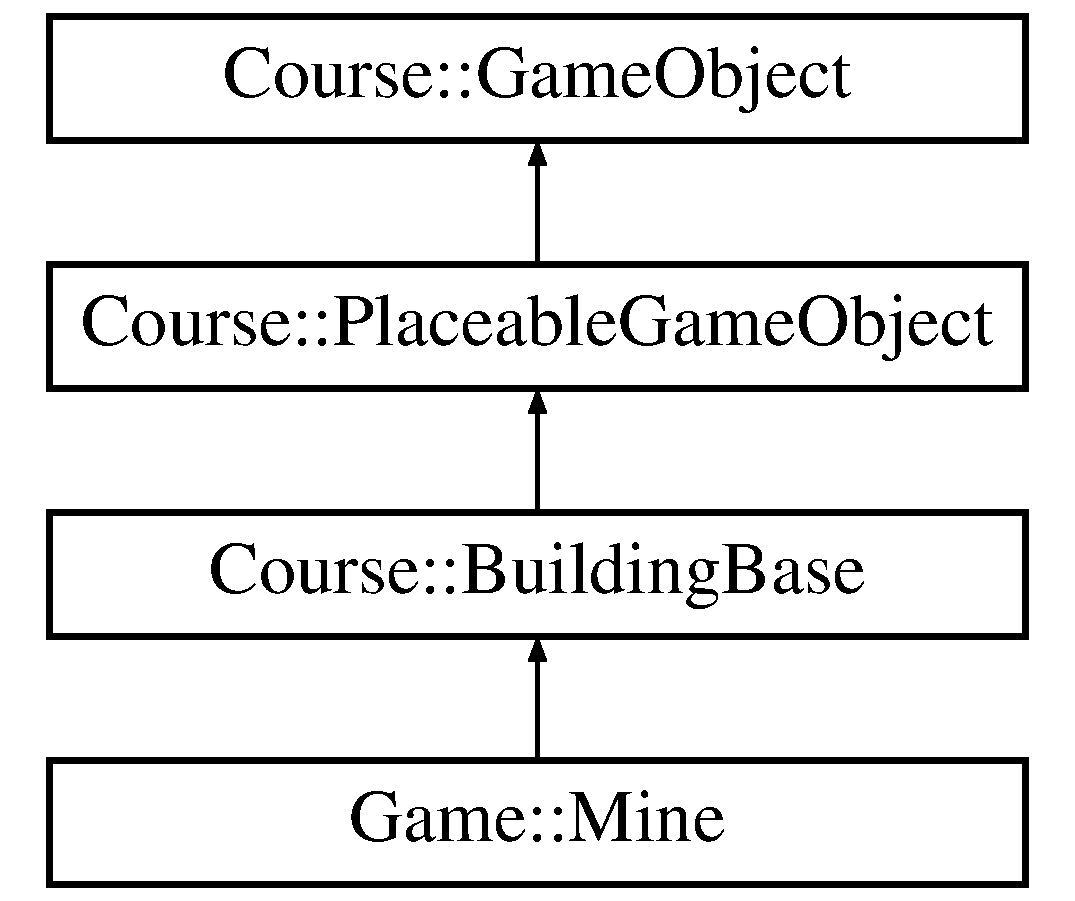
\includegraphics[height=4.000000cm]{classGame_1_1Mine}
\end{center}
\end{figure}
\subsection*{Public Member Functions}
\begin{DoxyCompactItemize}
\item 
\hyperlink{classGame_1_1Mine_a052f5f30bddf99dfeb2d5a250f052571}{Mine} ()=delete
\begin{DoxyCompactList}\small\item\em Disabled parameterless constructor. \end{DoxyCompactList}\item 
\hyperlink{classGame_1_1Mine_a47b233fda9aeb633a0de2e72c6030f1b}{Mine} (const std\-::shared\-\_\-ptr$<$ \hyperlink{classGame_1_1GameEventHandler}{Game\-Event\-Handler} $>$ \&eventhandler, const std\-::shared\-\_\-ptr$<$ \hyperlink{classGame_1_1ObjectManager}{Object\-Manager} $>$ \&objectmanager, const std\-::shared\-\_\-ptr$<$ \hyperlink{classGame_1_1Player}{Player} $>$ \&owner, const int \&tilespaces=1, const \hyperlink{namespaceCourse_ab9a46ed9cd00485e318e5731ea2f78d9}{Course\-::\-Resource\-Map} \&buildcost=\hyperlink{namespaceGame_1_1ConstResourceMaps_adda0aad5b2188a57d2d187f692e2c2f9}{Game\-::\-Const\-Resource\-Maps\-::\-M\-I\-N\-E\-\_\-\-B\-U\-I\-L\-D\-\_\-\-C\-O\-S\-T}, const \hyperlink{namespaceCourse_ab9a46ed9cd00485e318e5731ea2f78d9}{Course\-::\-Resource\-Map} \&production=\hyperlink{namespaceGame_1_1ConstResourceMaps_ad58736a7028bf9bdd46583af4cb3d410}{Game\-::\-Const\-Resource\-Maps\-::\-M\-I\-N\-E\-\_\-\-P\-R\-O\-D\-U\-C\-T\-I\-O\-N})
\begin{DoxyCompactList}\small\item\em Constructor for the class. \end{DoxyCompactList}\item 
virtual \hyperlink{classGame_1_1Mine_a418dd7de3691b762b7373e5f39a111c9}{$\sim$\-Mine} ()=default
\begin{DoxyCompactList}\small\item\em Default destructor. \end{DoxyCompactList}\item 
virtual std\-::string \hyperlink{classGame_1_1Mine_aaf18e426d1978c8e6f0cf0dc7435c257}{get\-Type} () const override
\end{DoxyCompactItemize}
\subsection*{Additional Inherited Members}


\subsection{Detailed Description}
The \hyperlink{classGame_1_1Mine}{Mine} class represents a mine-\/building in the game. 

The mine adds 1 base-\/production for money and 5 for stone and ore. 

\subsection{Constructor \& Destructor Documentation}
\hypertarget{classGame_1_1Mine_a052f5f30bddf99dfeb2d5a250f052571}{\index{Game\-::\-Mine@{Game\-::\-Mine}!Mine@{Mine}}
\index{Mine@{Mine}!Game::Mine@{Game\-::\-Mine}}
\subsubsection[{Mine}]{\setlength{\rightskip}{0pt plus 5cm}Game\-::\-Mine\-::\-Mine (
\begin{DoxyParamCaption}
{}
\end{DoxyParamCaption}
)\hspace{0.3cm}{\ttfamily [delete]}}}\label{classGame_1_1Mine_a052f5f30bddf99dfeb2d5a250f052571}


Disabled parameterless constructor. 

\hypertarget{classGame_1_1Mine_a47b233fda9aeb633a0de2e72c6030f1b}{\index{Game\-::\-Mine@{Game\-::\-Mine}!Mine@{Mine}}
\index{Mine@{Mine}!Game::Mine@{Game\-::\-Mine}}
\subsubsection[{Mine}]{\setlength{\rightskip}{0pt plus 5cm}Game\-::\-Mine\-::\-Mine (
\begin{DoxyParamCaption}
\item[{const std\-::shared\-\_\-ptr$<$ {\bf Game\-Event\-Handler} $>$ \&}]{eventhandler, }
\item[{const std\-::shared\-\_\-ptr$<$ {\bf Object\-Manager} $>$ \&}]{objectmanager, }
\item[{const std\-::shared\-\_\-ptr$<$ {\bf Player} $>$ \&}]{owner, }
\item[{const int \&}]{tilespaces = {\ttfamily 1}, }
\item[{const {\bf Course\-::\-Resource\-Map} \&}]{buildcost = {\ttfamily {\bf Game\-::\-Const\-Resource\-Maps\-::\-M\-I\-N\-E\-\_\-\-B\-U\-I\-L\-D\-\_\-\-C\-O\-S\-T}}, }
\item[{const {\bf Course\-::\-Resource\-Map} \&}]{production = {\ttfamily {\bf Game\-::\-Const\-Resource\-Maps\-::\-M\-I\-N\-E\-\_\-\-P\-R\-O\-D\-U\-C\-T\-I\-O\-N}}}
\end{DoxyParamCaption}
)\hspace{0.3cm}{\ttfamily [explicit]}}}\label{classGame_1_1Mine_a47b233fda9aeb633a0de2e72c6030f1b}


Constructor for the class. 


\begin{DoxyParams}{Parameters}
{\em eventhandler} & points to the student's \hyperlink{classGame_1_1GameEventHandler}{Game\-Event\-Handler}. \\
\hline
{\em owner} & points to the owning player. \\
\hline
{\em tile} & points to the tile upon which the building is constructed.\\
\hline
\end{DoxyParams}
\begin{DoxyPostcond}{Postcondition}
Exception Guarantee\-: No guarantee. 
\end{DoxyPostcond}

\begin{DoxyExceptions}{Exceptions}
{\em Owner\-Conflict} & -\/ if the building conflicts with tile's ownership. \\
\hline
\end{DoxyExceptions}
\hypertarget{classGame_1_1Mine_a418dd7de3691b762b7373e5f39a111c9}{\index{Game\-::\-Mine@{Game\-::\-Mine}!$\sim$\-Mine@{$\sim$\-Mine}}
\index{$\sim$\-Mine@{$\sim$\-Mine}!Game::Mine@{Game\-::\-Mine}}
\subsubsection[{$\sim$\-Mine}]{\setlength{\rightskip}{0pt plus 5cm}virtual Game\-::\-Mine\-::$\sim$\-Mine (
\begin{DoxyParamCaption}
{}
\end{DoxyParamCaption}
)\hspace{0.3cm}{\ttfamily [virtual]}, {\ttfamily [default]}}}\label{classGame_1_1Mine_a418dd7de3691b762b7373e5f39a111c9}


Default destructor. 



\subsection{Member Function Documentation}
\hypertarget{classGame_1_1Mine_aaf18e426d1978c8e6f0cf0dc7435c257}{\index{Game\-::\-Mine@{Game\-::\-Mine}!get\-Type@{get\-Type}}
\index{get\-Type@{get\-Type}!Game::Mine@{Game\-::\-Mine}}
\subsubsection[{get\-Type}]{\setlength{\rightskip}{0pt plus 5cm}std\-::string Game\-::\-Mine\-::get\-Type (
\begin{DoxyParamCaption}
{}
\end{DoxyParamCaption}
) const\hspace{0.3cm}{\ttfamily [override]}, {\ttfamily [virtual]}}}\label{classGame_1_1Mine_aaf18e426d1978c8e6f0cf0dc7435c257}






Reimplemented from \hyperlink{classCourse_1_1BuildingBase_ac2cc44e08dc73d05b1617bf71295baaf}{Course\-::\-Building\-Base}.



The documentation for this class was generated from the following files\-:\begin{DoxyCompactItemize}
\item 
Game/buildings/\hyperlink{mine_8hh}{mine.\-hh}\item 
Game/buildings/\hyperlink{mine_8cpp}{mine.\-cpp}\end{DoxyCompactItemize}

\hypertarget{classGame_1_1MineWorker}{\section{Game\-:\-:Mine\-Worker Class Reference}
\label{classGame_1_1MineWorker}\index{Game\-::\-Mine\-Worker@{Game\-::\-Mine\-Worker}}
}


The \hyperlink{classGame_1_1MineWorker}{Mine\-Worker} class represents a mine worker in the game.  




{\ttfamily \#include $<$mineworker.\-h$>$}

Inheritance diagram for Game\-:\-:Mine\-Worker\-:\begin{figure}[H]
\begin{center}
\leavevmode
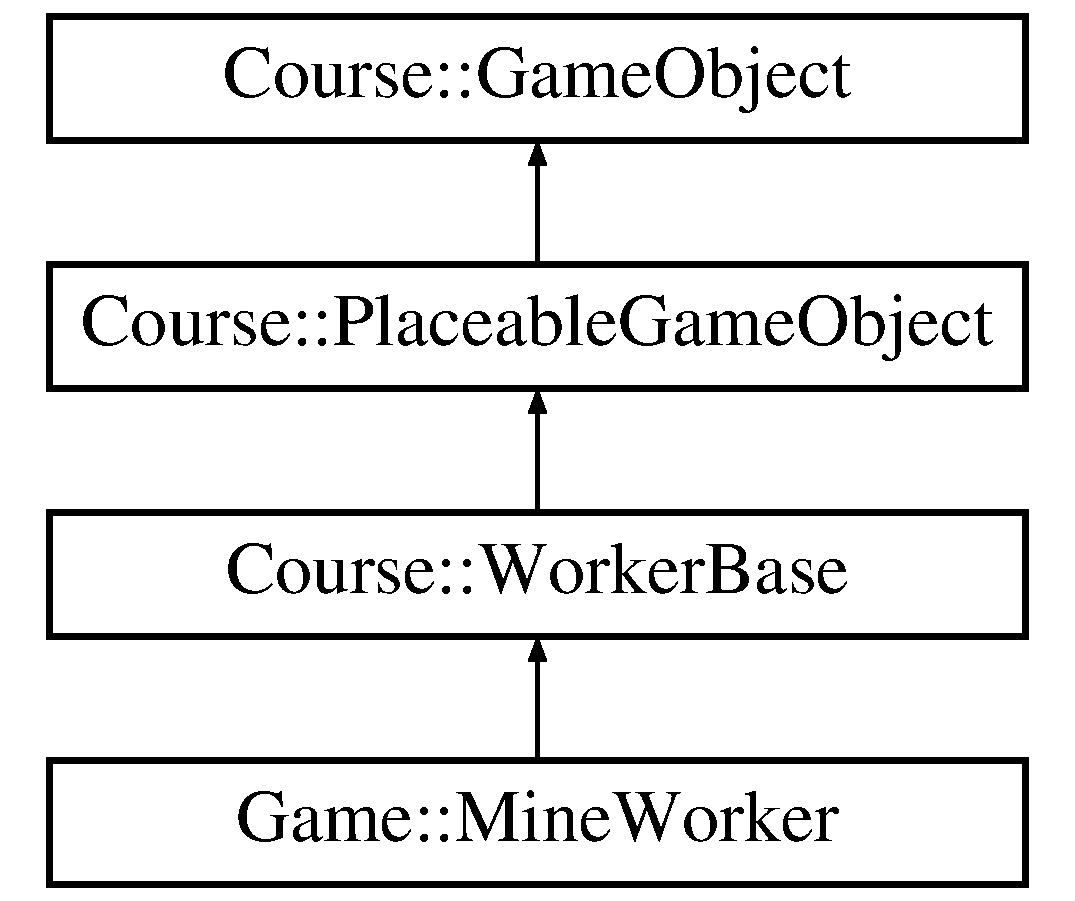
\includegraphics[height=4.000000cm]{classGame_1_1MineWorker}
\end{center}
\end{figure}
\subsection*{Public Member Functions}
\begin{DoxyCompactItemize}
\item 
\hyperlink{classGame_1_1MineWorker_a1b8706b2cbc8b5f84140230e432c8250}{Mine\-Worker} ()=delete
\begin{DoxyCompactList}\small\item\em Disabled parameterless constructor. \end{DoxyCompactList}\item 
\hyperlink{classGame_1_1MineWorker_a2d34cfd55b44b6012d9029ea66e8a7b4}{Mine\-Worker} (const std\-::shared\-\_\-ptr$<$ \hyperlink{classCourse_1_1iGameEventHandler}{Course\-::i\-Game\-Event\-Handler} $>$ \&eventhandler, const std\-::shared\-\_\-ptr$<$ \hyperlink{classCourse_1_1iObjectManager}{Course\-::i\-Object\-Manager} $>$ \&objectmanager, const std\-::shared\-\_\-ptr$<$ \hyperlink{classCourse_1_1PlayerBase}{Course\-::\-Player\-Base} $>$ \&owner, const int \&tilespaces=1, const \hyperlink{namespaceCourse_ab9a46ed9cd00485e318e5731ea2f78d9}{Course\-::\-Resource\-Map} \&cost=\hyperlink{namespaceGame_1_1ConstResourceMaps_ad5d316811f8c8442f6c24b5dc9134a87}{Game\-::\-Const\-Resource\-Maps\-::\-M\-W\-\_\-\-R\-E\-C\-R\-U\-I\-T\-M\-E\-N\-T\-\_\-\-C\-O\-S\-T}, const \hyperlink{namespaceCourse_a0b96bae1a664dde34efbb1b42dea615e}{Course\-::\-Resource\-Map\-Double} \&efficiency=\hyperlink{namespaceGame_1_1ConstResourceMaps_a11fc543cda6cf6dbd703559e230eb49a}{Game\-::\-Const\-Resource\-Maps\-::\-M\-W\-\_\-\-W\-O\-R\-K\-E\-R\-\_\-\-E\-F\-F\-I\-C\-I\-E\-N\-C\-Y})
\begin{DoxyCompactList}\small\item\em Constructor for the class. \end{DoxyCompactList}\item 
virtual \hyperlink{classGame_1_1MineWorker_a07f3a09a2c95491de57f1511a8162c43}{$\sim$\-Mine\-Worker} ()=default
\begin{DoxyCompactList}\small\item\em Default destructor. \end{DoxyCompactList}\item 
virtual std\-::string \hyperlink{classGame_1_1MineWorker_a984c2ede11ac50460620a4d982249dbe}{get\-Type} () const override
\item 
virtual bool \hyperlink{classGame_1_1MineWorker_aa52833ec99f6746871a78467c51bc57e}{can\-Be\-Placed\-On\-Tile} (const std\-::shared\-\_\-ptr$<$ \hyperlink{classCourse_1_1TileBase}{Course\-::\-Tile\-Base} $>$ \&target) const override
\begin{DoxyCompactList}\small\item\em Check if the worker can be placed on the Tile according to it's placement rule. Only rule is that the Tile must have same owner as the worker. \end{DoxyCompactList}\item 
virtual void \hyperlink{classGame_1_1MineWorker_a5faef20674a0d6408115461032e32edf}{do\-Special\-Action} () override
\begin{DoxyCompactList}\small\item\em Performs the Worker's default action. Does nothing as this is not implemented. \end{DoxyCompactList}\item 
virtual const \\*
\hyperlink{namespaceCourse_a0b96bae1a664dde34efbb1b42dea615e}{Course\-::\-Resource\-Map\-Double} \hyperlink{classGame_1_1MineWorker_a515a32b59f08ee1577210887166dacb0}{tile\-Work\-Action} () override
\begin{DoxyCompactList}\small\item\em Returns Worker's efficiency at resource production. Worker consumes F\-O\-O\-D and M\-O\-N\-E\-Y. Resource consumption and resource focus determine final multiplier that is based on W\-O\-R\-K\-E\-R\-\_\-\-E\-F\-F\-I\-C\-I\-E\-N\-C\-Y. \end{DoxyCompactList}\end{DoxyCompactItemize}
\subsection*{Additional Inherited Members}


\subsection{Detailed Description}
The \hyperlink{classGame_1_1MineWorker}{Mine\-Worker} class represents a mine worker in the game. 

Worker has following production-\/efficiency\-: \par

\begin{DoxyItemize}
\item Money -\/ 0.\-25 \par

\item Food -\/ 0.\-25 \par

\item Wood -\/ 0.\-25 \par

\item Stone -\/ 1.\-50 \par

\item Ore -\/ 1.\-50 \par
 Mine\-Workers consume Food and money. \par

\item 2 Food -\/ Or \hyperlink{classGame_1_1MineWorker}{Mine\-Worker} refuses to work. \par

\item 2 Money -\/ Or \hyperlink{classGame_1_1MineWorker}{Mine\-Worker} works at 50\% efficiency. 
\end{DoxyItemize}

\subsection{Constructor \& Destructor Documentation}
\hypertarget{classGame_1_1MineWorker_a1b8706b2cbc8b5f84140230e432c8250}{\index{Game\-::\-Mine\-Worker@{Game\-::\-Mine\-Worker}!Mine\-Worker@{Mine\-Worker}}
\index{Mine\-Worker@{Mine\-Worker}!Game::MineWorker@{Game\-::\-Mine\-Worker}}
\subsubsection[{Mine\-Worker}]{\setlength{\rightskip}{0pt plus 5cm}Game\-::\-Mine\-Worker\-::\-Mine\-Worker (
\begin{DoxyParamCaption}
{}
\end{DoxyParamCaption}
)\hspace{0.3cm}{\ttfamily [delete]}}}\label{classGame_1_1MineWorker_a1b8706b2cbc8b5f84140230e432c8250}


Disabled parameterless constructor. 

\hypertarget{classGame_1_1MineWorker_a2d34cfd55b44b6012d9029ea66e8a7b4}{\index{Game\-::\-Mine\-Worker@{Game\-::\-Mine\-Worker}!Mine\-Worker@{Mine\-Worker}}
\index{Mine\-Worker@{Mine\-Worker}!Game::MineWorker@{Game\-::\-Mine\-Worker}}
\subsubsection[{Mine\-Worker}]{\setlength{\rightskip}{0pt plus 5cm}Game\-::\-Mine\-Worker\-::\-Mine\-Worker (
\begin{DoxyParamCaption}
\item[{const std\-::shared\-\_\-ptr$<$ {\bf Course\-::i\-Game\-Event\-Handler} $>$ \&}]{eventhandler, }
\item[{const std\-::shared\-\_\-ptr$<$ {\bf Course\-::i\-Object\-Manager} $>$ \&}]{objectmanager, }
\item[{const std\-::shared\-\_\-ptr$<$ {\bf Course\-::\-Player\-Base} $>$ \&}]{owner, }
\item[{const int \&}]{tilespaces = {\ttfamily 1}, }
\item[{const {\bf Course\-::\-Resource\-Map} \&}]{cost = {\ttfamily {\bf Game\-::\-Const\-Resource\-Maps\-::\-M\-W\-\_\-\-R\-E\-C\-R\-U\-I\-T\-M\-E\-N\-T\-\_\-\-C\-O\-S\-T}}, }
\item[{const {\bf Course\-::\-Resource\-Map\-Double} \&}]{efficiency = {\ttfamily {\bf Game\-::\-Const\-Resource\-Maps\-::\-M\-W\-\_\-\-W\-O\-R\-K\-E\-R\-\_\-\-E\-F\-F\-I\-C\-I\-E\-N\-C\-Y}}}
\end{DoxyParamCaption}
)}}\label{classGame_1_1MineWorker_a2d34cfd55b44b6012d9029ea66e8a7b4}


Constructor for the class. 


\begin{DoxyParams}{Parameters}
{\em eventhandler} & points to the student's \hyperlink{classGame_1_1GameEventHandler}{Game\-Event\-Handler}. \\
\hline
{\em objectmanager} & points to the \hyperlink{classGame_1_1ObjectManager}{Object\-Manager}. \\
\hline
{\em owner} & points to the owning player. \\
\hline
{\em tilespaces} & defines how many spaces the worker takes on tile \\
\hline
{\em cost} & defines how much the worker costs \\
\hline
{\em efficiency} & defines how much and what the worker produces \\
\hline
\end{DoxyParams}
\hypertarget{classGame_1_1MineWorker_a07f3a09a2c95491de57f1511a8162c43}{\index{Game\-::\-Mine\-Worker@{Game\-::\-Mine\-Worker}!$\sim$\-Mine\-Worker@{$\sim$\-Mine\-Worker}}
\index{$\sim$\-Mine\-Worker@{$\sim$\-Mine\-Worker}!Game::MineWorker@{Game\-::\-Mine\-Worker}}
\subsubsection[{$\sim$\-Mine\-Worker}]{\setlength{\rightskip}{0pt plus 5cm}virtual Game\-::\-Mine\-Worker\-::$\sim$\-Mine\-Worker (
\begin{DoxyParamCaption}
{}
\end{DoxyParamCaption}
)\hspace{0.3cm}{\ttfamily [virtual]}, {\ttfamily [default]}}}\label{classGame_1_1MineWorker_a07f3a09a2c95491de57f1511a8162c43}


Default destructor. 



\subsection{Member Function Documentation}
\hypertarget{classGame_1_1MineWorker_aa52833ec99f6746871a78467c51bc57e}{\index{Game\-::\-Mine\-Worker@{Game\-::\-Mine\-Worker}!can\-Be\-Placed\-On\-Tile@{can\-Be\-Placed\-On\-Tile}}
\index{can\-Be\-Placed\-On\-Tile@{can\-Be\-Placed\-On\-Tile}!Game::MineWorker@{Game\-::\-Mine\-Worker}}
\subsubsection[{can\-Be\-Placed\-On\-Tile}]{\setlength{\rightskip}{0pt plus 5cm}bool Game\-::\-Mine\-Worker\-::can\-Be\-Placed\-On\-Tile (
\begin{DoxyParamCaption}
\item[{const std\-::shared\-\_\-ptr$<$ {\bf Course\-::\-Tile\-Base} $>$ \&}]{target}
\end{DoxyParamCaption}
) const\hspace{0.3cm}{\ttfamily [override]}, {\ttfamily [virtual]}}}\label{classGame_1_1MineWorker_aa52833ec99f6746871a78467c51bc57e}


Check if the worker can be placed on the Tile according to it's placement rule. Only rule is that the Tile must have same owner as the worker. 


\begin{DoxyParams}{Parameters}
{\em target} & is the Tile that worker is being placed on. \\
\hline
\end{DoxyParams}
\begin{DoxyReturn}{Returns}
True -\/ If baseclass' method return true and target Tile has space for worker. False -\/ If both conditions aren't met. 
\end{DoxyReturn}
\begin{DoxyNote}{Note}
Override to change placement rules for derived worker. 
\end{DoxyNote}
\begin{DoxyPostcond}{Postcondition}
Exception guarantee\-: Basic 
\end{DoxyPostcond}


Reimplemented from \hyperlink{classCourse_1_1WorkerBase_ad80874970ab91bca95b9d3f959e838d2}{Course\-::\-Worker\-Base}.

\hypertarget{classGame_1_1MineWorker_a5faef20674a0d6408115461032e32edf}{\index{Game\-::\-Mine\-Worker@{Game\-::\-Mine\-Worker}!do\-Special\-Action@{do\-Special\-Action}}
\index{do\-Special\-Action@{do\-Special\-Action}!Game::MineWorker@{Game\-::\-Mine\-Worker}}
\subsubsection[{do\-Special\-Action}]{\setlength{\rightskip}{0pt plus 5cm}void Game\-::\-Mine\-Worker\-::do\-Special\-Action (
\begin{DoxyParamCaption}
{}
\end{DoxyParamCaption}
)\hspace{0.3cm}{\ttfamily [override]}, {\ttfamily [virtual]}}}\label{classGame_1_1MineWorker_a5faef20674a0d6408115461032e32edf}


Performs the Worker's default action. Does nothing as this is not implemented. 



Implements \hyperlink{classCourse_1_1WorkerBase_a78553f35740e1c07d8f1071b5fc82212}{Course\-::\-Worker\-Base}.

\hypertarget{classGame_1_1MineWorker_a984c2ede11ac50460620a4d982249dbe}{\index{Game\-::\-Mine\-Worker@{Game\-::\-Mine\-Worker}!get\-Type@{get\-Type}}
\index{get\-Type@{get\-Type}!Game::MineWorker@{Game\-::\-Mine\-Worker}}
\subsubsection[{get\-Type}]{\setlength{\rightskip}{0pt plus 5cm}std\-::string Game\-::\-Mine\-Worker\-::get\-Type (
\begin{DoxyParamCaption}
{}
\end{DoxyParamCaption}
) const\hspace{0.3cm}{\ttfamily [override]}, {\ttfamily [virtual]}}}\label{classGame_1_1MineWorker_a984c2ede11ac50460620a4d982249dbe}






Reimplemented from \hyperlink{classCourse_1_1WorkerBase_afe6049810eec47fffe2c2a7334564ef9}{Course\-::\-Worker\-Base}.

\hypertarget{classGame_1_1MineWorker_a515a32b59f08ee1577210887166dacb0}{\index{Game\-::\-Mine\-Worker@{Game\-::\-Mine\-Worker}!tile\-Work\-Action@{tile\-Work\-Action}}
\index{tile\-Work\-Action@{tile\-Work\-Action}!Game::MineWorker@{Game\-::\-Mine\-Worker}}
\subsubsection[{tile\-Work\-Action}]{\setlength{\rightskip}{0pt plus 5cm}const {\bf Course\-::\-Resource\-Map\-Double} Game\-::\-Mine\-Worker\-::tile\-Work\-Action (
\begin{DoxyParamCaption}
{}
\end{DoxyParamCaption}
)\hspace{0.3cm}{\ttfamily [override]}, {\ttfamily [virtual]}}}\label{classGame_1_1MineWorker_a515a32b59f08ee1577210887166dacb0}


Returns Worker's efficiency at resource production. Worker consumes F\-O\-O\-D and M\-O\-N\-E\-Y. Resource consumption and resource focus determine final multiplier that is based on W\-O\-R\-K\-E\-R\-\_\-\-E\-F\-F\-I\-C\-I\-E\-N\-C\-Y. 

\begin{DoxyReturn}{Returns}

\end{DoxyReturn}


Reimplemented from \hyperlink{classCourse_1_1WorkerBase_af0c1bb4f3bbea015e2a55aa6eff7f9ae}{Course\-::\-Worker\-Base}.



The documentation for this class was generated from the following files\-:\begin{DoxyCompactItemize}
\item 
Game/workers/\hyperlink{mineworker_8h}{mineworker.\-h}\item 
Game/workers/\hyperlink{mineworker_8cpp}{mineworker.\-cpp}\end{DoxyCompactItemize}

\hypertarget{classCourse_1_1NotEnoughSpace}{\section{Course\-:\-:Not\-Enough\-Space Class Reference}
\label{classCourse_1_1NotEnoughSpace}\index{Course\-::\-Not\-Enough\-Space@{Course\-::\-Not\-Enough\-Space}}
}


The \hyperlink{classCourse_1_1NotEnoughSpace}{Not\-Enough\-Space} class is an Exception-\/class for errors where Game\-Objects are being placed onto Tiles with no space available.  




{\ttfamily \#include $<$notenoughspace.\-h$>$}

Inheritance diagram for Course\-:\-:Not\-Enough\-Space\-:\begin{figure}[H]
\begin{center}
\leavevmode
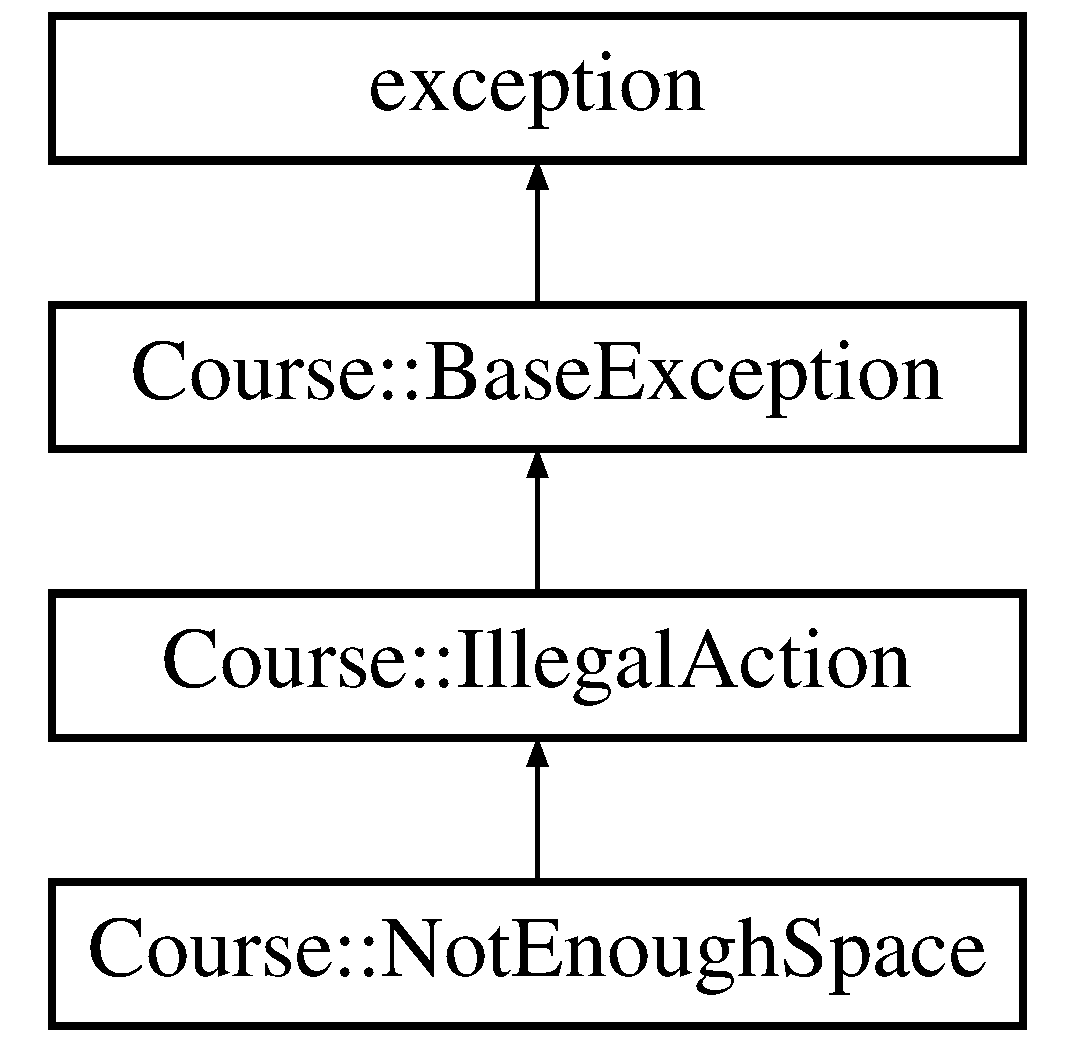
\includegraphics[height=4.000000cm]{classCourse_1_1NotEnoughSpace}
\end{center}
\end{figure}
\subsection*{Public Member Functions}
\begin{DoxyCompactItemize}
\item 
\hyperlink{classCourse_1_1NotEnoughSpace_a6dd4a0d6c0ed238b82b0cec97f9d70cf}{Not\-Enough\-Space} (const std\-::string \&\hyperlink{classCourse_1_1BaseException_ac5a744a6af6f2ba9198b58e52bb62f5a}{msg}=\char`\"{}\char`\"{})
\begin{DoxyCompactList}\small\item\em Exception Constructor. \end{DoxyCompactList}\item 
virtual \hyperlink{classCourse_1_1NotEnoughSpace_a14e18509490ee441d7dce6b72eb88428}{$\sim$\-Not\-Enough\-Space} ()=default
\begin{DoxyCompactList}\small\item\em $\sim$\-Exception Default destructor \end{DoxyCompactList}\end{DoxyCompactItemize}


\subsection{Detailed Description}
The \hyperlink{classCourse_1_1NotEnoughSpace}{Not\-Enough\-Space} class is an Exception-\/class for errors where Game\-Objects are being placed onto Tiles with no space available. 

\subsection{Constructor \& Destructor Documentation}
\hypertarget{classCourse_1_1NotEnoughSpace_a6dd4a0d6c0ed238b82b0cec97f9d70cf}{\index{Course\-::\-Not\-Enough\-Space@{Course\-::\-Not\-Enough\-Space}!Not\-Enough\-Space@{Not\-Enough\-Space}}
\index{Not\-Enough\-Space@{Not\-Enough\-Space}!Course::NotEnoughSpace@{Course\-::\-Not\-Enough\-Space}}
\subsubsection[{Not\-Enough\-Space}]{\setlength{\rightskip}{0pt plus 5cm}Course\-::\-Not\-Enough\-Space\-::\-Not\-Enough\-Space (
\begin{DoxyParamCaption}
\item[{const std\-::string \&}]{msg = {\ttfamily \char`\"{}\char`\"{}}}
\end{DoxyParamCaption}
)\hspace{0.3cm}{\ttfamily [inline]}, {\ttfamily [explicit]}}}\label{classCourse_1_1NotEnoughSpace_a6dd4a0d6c0ed238b82b0cec97f9d70cf}


Exception Constructor. 


\begin{DoxyParams}{Parameters}
{\em msg} & std\-::string describing the reason for exception. \\
\hline
\end{DoxyParams}
\hypertarget{classCourse_1_1NotEnoughSpace_a14e18509490ee441d7dce6b72eb88428}{\index{Course\-::\-Not\-Enough\-Space@{Course\-::\-Not\-Enough\-Space}!$\sim$\-Not\-Enough\-Space@{$\sim$\-Not\-Enough\-Space}}
\index{$\sim$\-Not\-Enough\-Space@{$\sim$\-Not\-Enough\-Space}!Course::NotEnoughSpace@{Course\-::\-Not\-Enough\-Space}}
\subsubsection[{$\sim$\-Not\-Enough\-Space}]{\setlength{\rightskip}{0pt plus 5cm}virtual Course\-::\-Not\-Enough\-Space\-::$\sim$\-Not\-Enough\-Space (
\begin{DoxyParamCaption}
{}
\end{DoxyParamCaption}
)\hspace{0.3cm}{\ttfamily [virtual]}, {\ttfamily [default]}}}\label{classCourse_1_1NotEnoughSpace_a14e18509490ee441d7dce6b72eb88428}


$\sim$\-Exception Default destructor 



The documentation for this class was generated from the following file\-:\begin{DoxyCompactItemize}
\item 
Course/\-Course\-Lib/exceptions/\hyperlink{notenoughspace_8h}{notenoughspace.\-h}\end{DoxyCompactItemize}

\hypertarget{classGame_1_1ObjectManager}{\section{Game\-:\-:Object\-Manager Class Reference}
\label{classGame_1_1ObjectManager}\index{Game\-::\-Object\-Manager@{Game\-::\-Object\-Manager}}
}


The \hyperlink{classGame_1_1ObjectManager}{Object\-Manager} class stores Players and Game\-Objects \par
(Tiles, Buildings and workers).  




{\ttfamily \#include $<$objectmanager.\-h$>$}

Inheritance diagram for Game\-:\-:Object\-Manager\-:\begin{figure}[H]
\begin{center}
\leavevmode
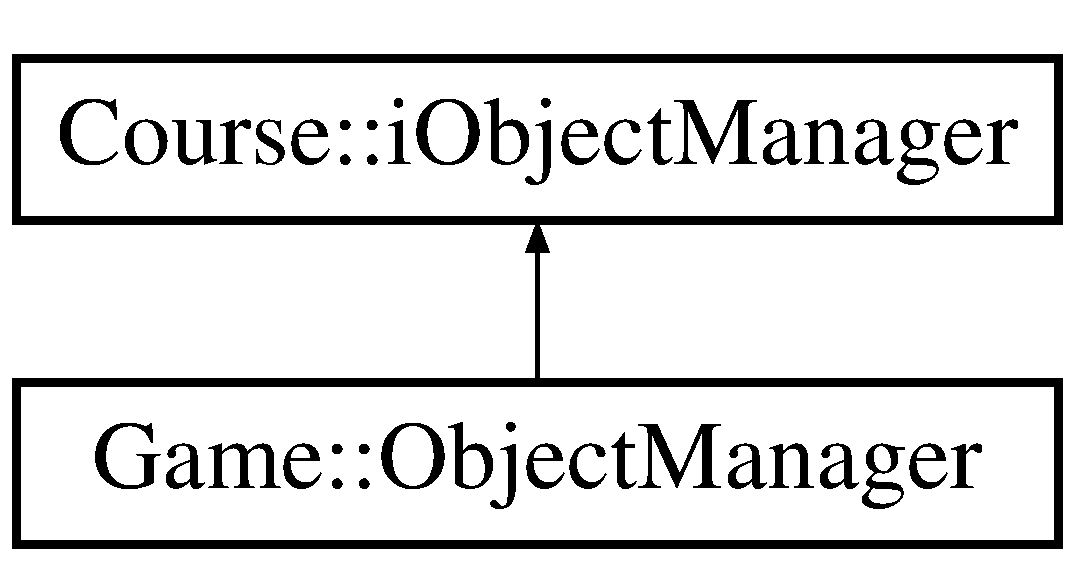
\includegraphics[height=2.000000cm]{classGame_1_1ObjectManager}
\end{center}
\end{figure}
\subsection*{Public Member Functions}
\begin{DoxyCompactItemize}
\item 
\hyperlink{classGame_1_1ObjectManager_a3f115e31fadbd2c0e3fbde6715d1bed3}{Object\-Manager} ()
\begin{DoxyCompactList}\small\item\em Constructor for the class. \end{DoxyCompactList}\item 
void \hyperlink{classGame_1_1ObjectManager_a92fb3bc8bebd8d08bf080ead20cfff10}{add\-Tiles} (const std\-::vector$<$ std\-::shared\-\_\-ptr$<$ \hyperlink{classCourse_1_1TileBase}{Course\-::\-Tile\-Base} $>$$>$ \&tiles)
\begin{DoxyCompactList}\small\item\em Adds new tiles to the \hyperlink{classGame_1_1ObjectManager}{Object\-Manager}. \end{DoxyCompactList}\item 
std\-::shared\-\_\-ptr$<$ \hyperlink{classCourse_1_1TileBase}{Course\-::\-Tile\-Base} $>$ \hyperlink{classGame_1_1ObjectManager_a0d1b58925d8baca124f611a697ea987c}{get\-Tile} (const \hyperlink{classCourse_1_1Coordinate}{Course\-::\-Coordinate} \&coordinate)
\begin{DoxyCompactList}\small\item\em Returns a shared pointer to a Tile that has specified coordinate. \end{DoxyCompactList}\item 
std\-::shared\-\_\-ptr$<$ \hyperlink{classCourse_1_1TileBase}{Course\-::\-Tile\-Base} $>$ \hyperlink{classGame_1_1ObjectManager_a299c9708f9e405d78a10b0aa7d1658aa}{get\-Tile} (const \hyperlink{namespaceCourse_a9a16e743c9813da00109e4991afd2f3e}{Course\-::\-Object\-Id} \&id)
\begin{DoxyCompactList}\small\item\em Returns a shared pointer to a Tile that has specified I\-D. \end{DoxyCompactList}\item 
std\-::vector$<$ std\-::shared\-\_\-ptr\\*
$<$ \hyperlink{classCourse_1_1TileBase}{Course\-::\-Tile\-Base} $>$ $>$ \hyperlink{classGame_1_1ObjectManager_ad4646477bd85b931f028a1a8f5916f3e}{get\-Tiles} (const std\-::vector$<$ \hyperlink{classCourse_1_1Coordinate}{Course\-::\-Coordinate} $>$ \&coordinates)
\begin{DoxyCompactList}\small\item\em Returns a vector of shared pointers to Tiles specified by a vector of Coordinates. \end{DoxyCompactList}\item 
const std\-::vector\\*
$<$ std\-::shared\-\_\-ptr\\*
$<$ \hyperlink{classCourse_1_1TileBase}{Course\-::\-Tile\-Base} $>$ $>$ \hyperlink{classGame_1_1ObjectManager_a76735d2c025272c4da5b0d31de95074f}{get\-Tiles} () const 
\begin{DoxyCompactList}\small\item\em Returns a vector of shared pointers to all stored Tiles. \end{DoxyCompactList}\item 
void \hyperlink{classGame_1_1ObjectManager_a6b3912ce2a0227612415fc8df1b22ca4}{add\-Player} (const std\-::shared\-\_\-ptr$<$ \hyperlink{classGame_1_1Player}{Player} $>$ player)
\begin{DoxyCompactList}\small\item\em Adds a new \hyperlink{classGame_1_1Player}{Player} to the \hyperlink{classGame_1_1ObjectManager}{Object\-Manager}. \end{DoxyCompactList}\item 
const std\-::vector\\*
$<$ std\-::shared\-\_\-ptr$<$ \hyperlink{classGame_1_1Player}{Player} $>$ $>$ \hyperlink{classGame_1_1ObjectManager_a5a61b66cbdbd0625b1cdc8a1934fb89b}{get\-Players} () const 
\begin{DoxyCompactList}\small\item\em Returns a vector of shared pointers to all stored Players. \end{DoxyCompactList}\item 
bool \hyperlink{classGame_1_1ObjectManager_a4a20ffcde5447350bbf056fd21fb3cdd}{is\-Last\-Player} (const std\-::shared\-\_\-ptr$<$ \hyperlink{classGame_1_1Player}{Player} $>$ player)
\begin{DoxyCompactList}\small\item\em Returns whether a player is the last player to act. \end{DoxyCompactList}\item 
void \hyperlink{classGame_1_1ObjectManager_a6542f6244d107d2d5c84d644faa3cad3}{add\-Placeable\-Object} (const std\-::shared\-\_\-ptr$<$ \hyperlink{classCourse_1_1PlaceableGameObject}{Course\-::\-Placeable\-Game\-Object} $>$ object)
\begin{DoxyCompactList}\small\item\em Adds a new Placeable\-Game\-Object to the \hyperlink{classGame_1_1ObjectManager}{Object\-Manager}. \end{DoxyCompactList}\item 
const std\-::shared\-\_\-ptr\\*
$<$ \hyperlink{classCourse_1_1PlaceableGameObject}{Course\-::\-Placeable\-Game\-Object} $>$ \hyperlink{classGame_1_1ObjectManager_a5c0154e5add41fd11d1c0e36356ed4ef}{get\-Newest\-Placeable\-Object} ()
\begin{DoxyCompactList}\small\item\em Returns a shared pointer to a Placeable\-Game\-Object that \par
was last added. \end{DoxyCompactList}\end{DoxyCompactItemize}
\subsection*{Private Attributes}
\begin{DoxyCompactItemize}
\item 
std\-::vector$<$ std\-::shared\-\_\-ptr\\*
$<$ \hyperlink{classCourse_1_1TileBase}{Course\-::\-Tile\-Base} $>$ $>$ \hyperlink{classGame_1_1ObjectManager_a814f7a4ef4201c5627c0ae77a4a3dec1}{m\-\_\-tiles}
\item 
std\-::vector$<$ std\-::shared\-\_\-ptr\\*
$<$ \hyperlink{classGame_1_1Player}{Player} $>$ $>$ \hyperlink{classGame_1_1ObjectManager_ae4c88baa0dec114607b47da932b03243}{m\-\_\-players}
\item 
std\-::vector$<$ std\-::shared\-\_\-ptr\\*
$<$ \hyperlink{classCourse_1_1PlaceableGameObject}{Course\-::\-Placeable\-Game\-Object} $>$ $>$ \hyperlink{classGame_1_1ObjectManager_abba2ff9bea647e526ef9a556ebbbcdbe}{m\-\_\-placeable\-Objects}
\end{DoxyCompactItemize}


\subsection{Detailed Description}
The \hyperlink{classGame_1_1ObjectManager}{Object\-Manager} class stores Players and Game\-Objects \par
(Tiles, Buildings and workers). 

Only one of these should exists at any given point in the time 

\subsection{Constructor \& Destructor Documentation}
\hypertarget{classGame_1_1ObjectManager_a3f115e31fadbd2c0e3fbde6715d1bed3}{\index{Game\-::\-Object\-Manager@{Game\-::\-Object\-Manager}!Object\-Manager@{Object\-Manager}}
\index{Object\-Manager@{Object\-Manager}!Game::ObjectManager@{Game\-::\-Object\-Manager}}
\subsubsection[{Object\-Manager}]{\setlength{\rightskip}{0pt plus 5cm}Game\-::\-Object\-Manager\-::\-Object\-Manager (
\begin{DoxyParamCaption}
{}
\end{DoxyParamCaption}
)}}\label{classGame_1_1ObjectManager_a3f115e31fadbd2c0e3fbde6715d1bed3}


Constructor for the class. 



\subsection{Member Function Documentation}
\hypertarget{classGame_1_1ObjectManager_a6542f6244d107d2d5c84d644faa3cad3}{\index{Game\-::\-Object\-Manager@{Game\-::\-Object\-Manager}!add\-Placeable\-Object@{add\-Placeable\-Object}}
\index{add\-Placeable\-Object@{add\-Placeable\-Object}!Game::ObjectManager@{Game\-::\-Object\-Manager}}
\subsubsection[{add\-Placeable\-Object}]{\setlength{\rightskip}{0pt plus 5cm}void Game\-::\-Object\-Manager\-::add\-Placeable\-Object (
\begin{DoxyParamCaption}
\item[{const std\-::shared\-\_\-ptr$<$ {\bf Course\-::\-Placeable\-Game\-Object} $>$}]{object}
\end{DoxyParamCaption}
)}}\label{classGame_1_1ObjectManager_a6542f6244d107d2d5c84d644faa3cad3}


Adds a new Placeable\-Game\-Object to the \hyperlink{classGame_1_1ObjectManager}{Object\-Manager}. 


\begin{DoxyParams}{Parameters}
{\em object} & a pointer to a Placeable\-Game\-Object \\
\hline
\end{DoxyParams}
\begin{DoxyPostcond}{Postcondition}
The player-\/pointer is stored in the \hyperlink{classGame_1_1ObjectManager}{Object\-Manager}. Exception Guarantee\-: Basic 
\end{DoxyPostcond}
\hypertarget{classGame_1_1ObjectManager_a6b3912ce2a0227612415fc8df1b22ca4}{\index{Game\-::\-Object\-Manager@{Game\-::\-Object\-Manager}!add\-Player@{add\-Player}}
\index{add\-Player@{add\-Player}!Game::ObjectManager@{Game\-::\-Object\-Manager}}
\subsubsection[{add\-Player}]{\setlength{\rightskip}{0pt plus 5cm}void Game\-::\-Object\-Manager\-::add\-Player (
\begin{DoxyParamCaption}
\item[{const std\-::shared\-\_\-ptr$<$ {\bf Player} $>$}]{player}
\end{DoxyParamCaption}
)}}\label{classGame_1_1ObjectManager_a6b3912ce2a0227612415fc8df1b22ca4}


Adds a new \hyperlink{classGame_1_1Player}{Player} to the \hyperlink{classGame_1_1ObjectManager}{Object\-Manager}. 


\begin{DoxyParams}{Parameters}
{\em player} & a pointer to a \hyperlink{classGame_1_1Player}{Player} \\
\hline
\end{DoxyParams}
\begin{DoxyPostcond}{Postcondition}
The player-\/pointer is stored in the \hyperlink{classGame_1_1ObjectManager}{Object\-Manager}. Exception Guarantee\-: Basic 
\end{DoxyPostcond}
\hypertarget{classGame_1_1ObjectManager_a92fb3bc8bebd8d08bf080ead20cfff10}{\index{Game\-::\-Object\-Manager@{Game\-::\-Object\-Manager}!add\-Tiles@{add\-Tiles}}
\index{add\-Tiles@{add\-Tiles}!Game::ObjectManager@{Game\-::\-Object\-Manager}}
\subsubsection[{add\-Tiles}]{\setlength{\rightskip}{0pt plus 5cm}void Game\-::\-Object\-Manager\-::add\-Tiles (
\begin{DoxyParamCaption}
\item[{const std\-::vector$<$ std\-::shared\-\_\-ptr$<$ {\bf Course\-::\-Tile\-Base} $>$$>$ \&}]{tiles}
\end{DoxyParamCaption}
)\hspace{0.3cm}{\ttfamily [virtual]}}}\label{classGame_1_1ObjectManager_a92fb3bc8bebd8d08bf080ead20cfff10}


Adds new tiles to the \hyperlink{classGame_1_1ObjectManager}{Object\-Manager}. 


\begin{DoxyParams}{Parameters}
{\em tiles} & a vector that contains the Tiles to be added. \\
\hline
\end{DoxyParams}
\begin{DoxyPostcond}{Postcondition}
The tile-\/pointers in the vector are stored in the \hyperlink{classGame_1_1ObjectManager}{Object\-Manager}. Exception Guarantee\-: Basic 
\end{DoxyPostcond}


Implements \hyperlink{classCourse_1_1iObjectManager_a826fa55229bdc23c49f847245fbdda95}{Course\-::i\-Object\-Manager}.

\hypertarget{classGame_1_1ObjectManager_a5c0154e5add41fd11d1c0e36356ed4ef}{\index{Game\-::\-Object\-Manager@{Game\-::\-Object\-Manager}!get\-Newest\-Placeable\-Object@{get\-Newest\-Placeable\-Object}}
\index{get\-Newest\-Placeable\-Object@{get\-Newest\-Placeable\-Object}!Game::ObjectManager@{Game\-::\-Object\-Manager}}
\subsubsection[{get\-Newest\-Placeable\-Object}]{\setlength{\rightskip}{0pt plus 5cm}const std\-::shared\-\_\-ptr$<$ {\bf Course\-::\-Placeable\-Game\-Object} $>$ Game\-::\-Object\-Manager\-::get\-Newest\-Placeable\-Object (
\begin{DoxyParamCaption}
{}
\end{DoxyParamCaption}
)}}\label{classGame_1_1ObjectManager_a5c0154e5add41fd11d1c0e36356ed4ef}


Returns a shared pointer to a Placeable\-Game\-Object that \par
was last added. 

\begin{DoxyReturn}{Returns}
a pointer to a Placeable\-Game\-Object that was last added 
\end{DoxyReturn}
\begin{DoxyPostcond}{Postcondition}
Exception Guarantee\-: Basic 
\end{DoxyPostcond}
\hypertarget{classGame_1_1ObjectManager_a5a61b66cbdbd0625b1cdc8a1934fb89b}{\index{Game\-::\-Object\-Manager@{Game\-::\-Object\-Manager}!get\-Players@{get\-Players}}
\index{get\-Players@{get\-Players}!Game::ObjectManager@{Game\-::\-Object\-Manager}}
\subsubsection[{get\-Players}]{\setlength{\rightskip}{0pt plus 5cm}const std\-::vector$<$ std\-::shared\-\_\-ptr$<$ {\bf Player} $>$ $>$ Game\-::\-Object\-Manager\-::get\-Players (
\begin{DoxyParamCaption}
{}
\end{DoxyParamCaption}
) const}}\label{classGame_1_1ObjectManager_a5a61b66cbdbd0625b1cdc8a1934fb89b}


Returns a vector of shared pointers to all stored Players. 

\begin{DoxyReturn}{Returns}
Vector that contains pointers to Players 
\end{DoxyReturn}
\begin{DoxyPostcond}{Postcondition}
Exception Guarantee\-: Basic 
\end{DoxyPostcond}
\hypertarget{classGame_1_1ObjectManager_a0d1b58925d8baca124f611a697ea987c}{\index{Game\-::\-Object\-Manager@{Game\-::\-Object\-Manager}!get\-Tile@{get\-Tile}}
\index{get\-Tile@{get\-Tile}!Game::ObjectManager@{Game\-::\-Object\-Manager}}
\subsubsection[{get\-Tile}]{\setlength{\rightskip}{0pt plus 5cm}std\-::shared\-\_\-ptr$<$ {\bf Course\-::\-Tile\-Base} $>$ Game\-::\-Object\-Manager\-::get\-Tile (
\begin{DoxyParamCaption}
\item[{const {\bf Course\-::\-Coordinate} \&}]{coordinate}
\end{DoxyParamCaption}
)\hspace{0.3cm}{\ttfamily [virtual]}}}\label{classGame_1_1ObjectManager_a0d1b58925d8baca124f611a697ea987c}


Returns a shared pointer to a Tile that has specified coordinate. 


\begin{DoxyParams}{Parameters}
{\em coordinate} & Requested Tile's Coordinate \\
\hline
\end{DoxyParams}
\begin{DoxyReturn}{Returns}
a pointer to a Tile that has the given coordinate. If no for the coordinate exists, return empty pointer. 
\end{DoxyReturn}
\begin{DoxyPostcond}{Postcondition}
Exception Guarantee\-: Basic 
\end{DoxyPostcond}


Implements \hyperlink{classCourse_1_1iObjectManager_afd7ab74d8a4cfedd50340c1e9096672d}{Course\-::i\-Object\-Manager}.

\hypertarget{classGame_1_1ObjectManager_a299c9708f9e405d78a10b0aa7d1658aa}{\index{Game\-::\-Object\-Manager@{Game\-::\-Object\-Manager}!get\-Tile@{get\-Tile}}
\index{get\-Tile@{get\-Tile}!Game::ObjectManager@{Game\-::\-Object\-Manager}}
\subsubsection[{get\-Tile}]{\setlength{\rightskip}{0pt plus 5cm}std\-::shared\-\_\-ptr$<$ {\bf Course\-::\-Tile\-Base} $>$ Game\-::\-Object\-Manager\-::get\-Tile (
\begin{DoxyParamCaption}
\item[{const {\bf Course\-::\-Object\-Id} \&}]{id}
\end{DoxyParamCaption}
)\hspace{0.3cm}{\ttfamily [virtual]}}}\label{classGame_1_1ObjectManager_a299c9708f9e405d78a10b0aa7d1658aa}


Returns a shared pointer to a Tile that has specified I\-D. 


\begin{DoxyParams}{Parameters}
{\em id} & Tile's Object\-Id. \\
\hline
\end{DoxyParams}
\begin{DoxyReturn}{Returns}
a pointer to the Tile that has the given I\-D If no for the id exists, return empty pointer. 
\end{DoxyReturn}
\begin{DoxyPostcond}{Postcondition}
Exception Guarantee\-: Basic 
\end{DoxyPostcond}


Implements \hyperlink{classCourse_1_1iObjectManager_a7c3280cc01c8cf77d49afe88ca0e6b48}{Course\-::i\-Object\-Manager}.

\hypertarget{classGame_1_1ObjectManager_ad4646477bd85b931f028a1a8f5916f3e}{\index{Game\-::\-Object\-Manager@{Game\-::\-Object\-Manager}!get\-Tiles@{get\-Tiles}}
\index{get\-Tiles@{get\-Tiles}!Game::ObjectManager@{Game\-::\-Object\-Manager}}
\subsubsection[{get\-Tiles}]{\setlength{\rightskip}{0pt plus 5cm}std\-::vector$<$ std\-::shared\-\_\-ptr$<$ {\bf Course\-::\-Tile\-Base} $>$ $>$ Game\-::\-Object\-Manager\-::get\-Tiles (
\begin{DoxyParamCaption}
\item[{const std\-::vector$<$ {\bf Course\-::\-Coordinate} $>$ \&}]{coordinates}
\end{DoxyParamCaption}
)\hspace{0.3cm}{\ttfamily [virtual]}}}\label{classGame_1_1ObjectManager_ad4646477bd85b931f028a1a8f5916f3e}


Returns a vector of shared pointers to Tiles specified by a vector of Coordinates. 


\begin{DoxyParams}{Parameters}
{\em coordinates} & a vector of Coordinates for the requested Tiles \\
\hline
\end{DoxyParams}
\begin{DoxyReturn}{Returns}
Vector of that contains pointers to Tile's that match the coordinates. The vector is empty if no matches were made. 
\end{DoxyReturn}
\begin{DoxyPostcond}{Postcondition}
Exception Guarantee\-: Basic 
\end{DoxyPostcond}


Implements \hyperlink{classCourse_1_1iObjectManager_ac1b0d805db508f80477fbb7e5987e4e4}{Course\-::i\-Object\-Manager}.

\hypertarget{classGame_1_1ObjectManager_a76735d2c025272c4da5b0d31de95074f}{\index{Game\-::\-Object\-Manager@{Game\-::\-Object\-Manager}!get\-Tiles@{get\-Tiles}}
\index{get\-Tiles@{get\-Tiles}!Game::ObjectManager@{Game\-::\-Object\-Manager}}
\subsubsection[{get\-Tiles}]{\setlength{\rightskip}{0pt plus 5cm}const std\-::vector$<$ std\-::shared\-\_\-ptr$<$ {\bf Course\-::\-Tile\-Base} $>$ $>$ Game\-::\-Object\-Manager\-::get\-Tiles (
\begin{DoxyParamCaption}
{}
\end{DoxyParamCaption}
) const}}\label{classGame_1_1ObjectManager_a76735d2c025272c4da5b0d31de95074f}


Returns a vector of shared pointers to all stored Tiles. 

\begin{DoxyReturn}{Returns}
Vector that contains pointers to Tiles 
\end{DoxyReturn}
\begin{DoxyPostcond}{Postcondition}
Exception Guarantee\-: Basic 
\end{DoxyPostcond}
\hypertarget{classGame_1_1ObjectManager_a4a20ffcde5447350bbf056fd21fb3cdd}{\index{Game\-::\-Object\-Manager@{Game\-::\-Object\-Manager}!is\-Last\-Player@{is\-Last\-Player}}
\index{is\-Last\-Player@{is\-Last\-Player}!Game::ObjectManager@{Game\-::\-Object\-Manager}}
\subsubsection[{is\-Last\-Player}]{\setlength{\rightskip}{0pt plus 5cm}bool Game\-::\-Object\-Manager\-::is\-Last\-Player (
\begin{DoxyParamCaption}
\item[{const std\-::shared\-\_\-ptr$<$ {\bf Player} $>$}]{player}
\end{DoxyParamCaption}
)}}\label{classGame_1_1ObjectManager_a4a20ffcde5447350bbf056fd21fb3cdd}


Returns whether a player is the last player to act. 


\begin{DoxyParams}{Parameters}
{\em player} & a pointer to a \hyperlink{classGame_1_1Player}{Player} \\
\hline
\end{DoxyParams}
\begin{DoxyReturn}{Returns}
Bool that tells if the player is last to act 
\end{DoxyReturn}
\begin{DoxyPostcond}{Postcondition}
Exception Guarantee\-: Basic 
\end{DoxyPostcond}


\subsection{Member Data Documentation}
\hypertarget{classGame_1_1ObjectManager_abba2ff9bea647e526ef9a556ebbbcdbe}{\index{Game\-::\-Object\-Manager@{Game\-::\-Object\-Manager}!m\-\_\-placeable\-Objects@{m\-\_\-placeable\-Objects}}
\index{m\-\_\-placeable\-Objects@{m\-\_\-placeable\-Objects}!Game::ObjectManager@{Game\-::\-Object\-Manager}}
\subsubsection[{m\-\_\-placeable\-Objects}]{\setlength{\rightskip}{0pt plus 5cm}std\-::vector$<$std\-::shared\-\_\-ptr$<${\bf Course\-::\-Placeable\-Game\-Object}$>$ $>$ Game\-::\-Object\-Manager\-::m\-\_\-placeable\-Objects\hspace{0.3cm}{\ttfamily [private]}}}\label{classGame_1_1ObjectManager_abba2ff9bea647e526ef9a556ebbbcdbe}
\hypertarget{classGame_1_1ObjectManager_ae4c88baa0dec114607b47da932b03243}{\index{Game\-::\-Object\-Manager@{Game\-::\-Object\-Manager}!m\-\_\-players@{m\-\_\-players}}
\index{m\-\_\-players@{m\-\_\-players}!Game::ObjectManager@{Game\-::\-Object\-Manager}}
\subsubsection[{m\-\_\-players}]{\setlength{\rightskip}{0pt plus 5cm}std\-::vector$<$std\-::shared\-\_\-ptr$<${\bf Player}$>$ $>$ Game\-::\-Object\-Manager\-::m\-\_\-players\hspace{0.3cm}{\ttfamily [private]}}}\label{classGame_1_1ObjectManager_ae4c88baa0dec114607b47da932b03243}
\hypertarget{classGame_1_1ObjectManager_a814f7a4ef4201c5627c0ae77a4a3dec1}{\index{Game\-::\-Object\-Manager@{Game\-::\-Object\-Manager}!m\-\_\-tiles@{m\-\_\-tiles}}
\index{m\-\_\-tiles@{m\-\_\-tiles}!Game::ObjectManager@{Game\-::\-Object\-Manager}}
\subsubsection[{m\-\_\-tiles}]{\setlength{\rightskip}{0pt plus 5cm}std\-::vector$<$std\-::shared\-\_\-ptr$<${\bf Course\-::\-Tile\-Base}$>$ $>$ Game\-::\-Object\-Manager\-::m\-\_\-tiles\hspace{0.3cm}{\ttfamily [private]}}}\label{classGame_1_1ObjectManager_a814f7a4ef4201c5627c0ae77a4a3dec1}


The documentation for this class was generated from the following files\-:\begin{DoxyCompactItemize}
\item 
Game/core/\hyperlink{objectmanager_8h}{objectmanager.\-h}\item 
Game/core/\hyperlink{objectmanager_8cpp}{objectmanager.\-cpp}\end{DoxyCompactItemize}

\hypertarget{classGame_1_1OreDeposit}{\section{Game\-:\-:Ore\-Deposit Class Reference}
\label{classGame_1_1OreDeposit}\index{Game\-::\-Ore\-Deposit@{Game\-::\-Ore\-Deposit}}
}


The \hyperlink{classGame_1_1OreDeposit}{Ore\-Deposit} class represents an ore deposit in the gameworld.  




{\ttfamily \#include $<$oredeposit.\-h$>$}

Inheritance diagram for Game\-:\-:Ore\-Deposit\-:\begin{figure}[H]
\begin{center}
\leavevmode
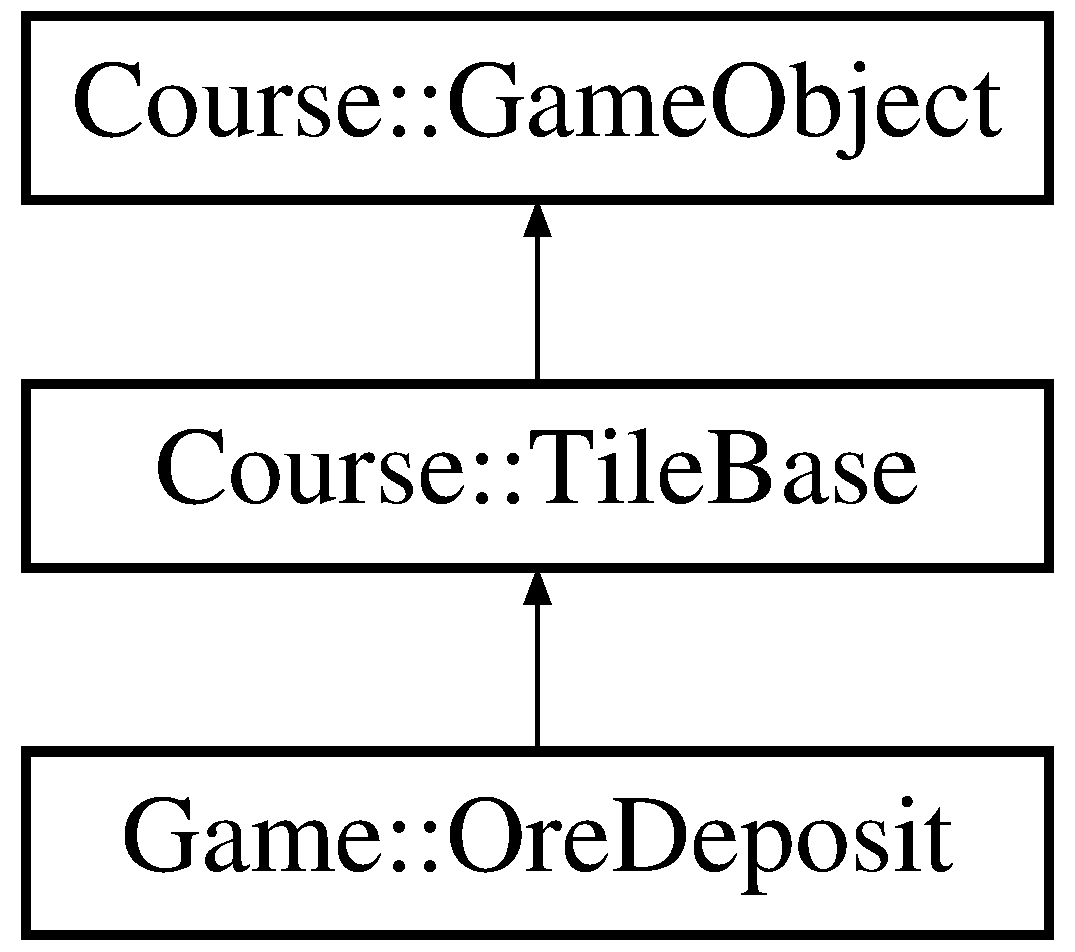
\includegraphics[height=3.000000cm]{classGame_1_1OreDeposit}
\end{center}
\end{figure}
\subsection*{Public Member Functions}
\begin{DoxyCompactItemize}
\item 
\hyperlink{classGame_1_1OreDeposit_a9e68e72e04c7525b24f6cf32b61f9df3}{Ore\-Deposit} ()=delete
\begin{DoxyCompactList}\small\item\em Disabled parameterless constructor. \end{DoxyCompactList}\item 
\hyperlink{classGame_1_1OreDeposit_a6377d7e3031a9011704d74324f003729}{Ore\-Deposit} (const \hyperlink{classCourse_1_1Coordinate}{Course\-::\-Coordinate} \&location, const std\-::shared\-\_\-ptr$<$ \hyperlink{classCourse_1_1iGameEventHandler}{Course\-::i\-Game\-Event\-Handler} $>$ \&eventhandler, const std\-::shared\-\_\-ptr$<$ \hyperlink{classCourse_1_1iObjectManager}{Course\-::i\-Object\-Manager} $>$ \&objectmanager, const unsigned int \&max\-\_\-build=2, const unsigned int \&max\-\_\-work=3, const \hyperlink{namespaceCourse_ab9a46ed9cd00485e318e5731ea2f78d9}{Course\-::\-Resource\-Map} \&production=\hyperlink{namespaceGame_1_1ConstResourceMaps_a7b803a949c1a3e044a6a6f985928a0cc}{Game\-::\-Const\-Resource\-Maps\-::\-O\-R\-E\-D\-E\-P\-O\-S\-I\-T\-\_\-\-B\-P})
\begin{DoxyCompactList}\small\item\em Constructor for the class. \end{DoxyCompactList}\item 
virtual \hyperlink{classGame_1_1OreDeposit_a2d397792fa3cb65c27b29061b1678bb9}{$\sim$\-Ore\-Deposit} ()=default
\begin{DoxyCompactList}\small\item\em Default destructor. \end{DoxyCompactList}\item 
virtual std\-::string \hyperlink{classGame_1_1OreDeposit_acc2ba331cb40a464821fe6ebaaf63573}{get\-Type} () const override
\item 
void \hyperlink{classGame_1_1OreDeposit_af8a88425e59e4fbb12eb90cc70b22ac7}{add\-Building} (const std\-::shared\-\_\-ptr$<$ \hyperlink{classCourse_1_1BuildingBase}{Course\-::\-Building\-Base} $>$ \&building) override
\begin{DoxyCompactList}\small\item\em Adds a new building-\/object to the tile. Building in ore deposit adds one hold-\/marker to the building. \end{DoxyCompactList}\end{DoxyCompactItemize}
\subsection*{Additional Inherited Members}


\subsection{Detailed Description}
The \hyperlink{classGame_1_1OreDeposit}{Ore\-Deposit} class represents an ore deposit in the gameworld. 

\hyperlink{classGame_1_1OreDeposit}{Ore\-Deposit} has Basic\-Production\-: \par

\begin{DoxyItemize}
\item Money = 3
\item Food = 0
\item Wood = 0
\item Stone = 2
\item Ore = 5
\end{DoxyItemize}

Building in the ore deposit takes time. So buildings get extra hold-\/marker.

Tile supports 2 buildings. 

\subsection{Constructor \& Destructor Documentation}
\hypertarget{classGame_1_1OreDeposit_a9e68e72e04c7525b24f6cf32b61f9df3}{\index{Game\-::\-Ore\-Deposit@{Game\-::\-Ore\-Deposit}!Ore\-Deposit@{Ore\-Deposit}}
\index{Ore\-Deposit@{Ore\-Deposit}!Game::OreDeposit@{Game\-::\-Ore\-Deposit}}
\subsubsection[{Ore\-Deposit}]{\setlength{\rightskip}{0pt plus 5cm}Game\-::\-Ore\-Deposit\-::\-Ore\-Deposit (
\begin{DoxyParamCaption}
{}
\end{DoxyParamCaption}
)\hspace{0.3cm}{\ttfamily [delete]}}}\label{classGame_1_1OreDeposit_a9e68e72e04c7525b24f6cf32b61f9df3}


Disabled parameterless constructor. 

\hypertarget{classGame_1_1OreDeposit_a6377d7e3031a9011704d74324f003729}{\index{Game\-::\-Ore\-Deposit@{Game\-::\-Ore\-Deposit}!Ore\-Deposit@{Ore\-Deposit}}
\index{Ore\-Deposit@{Ore\-Deposit}!Game::OreDeposit@{Game\-::\-Ore\-Deposit}}
\subsubsection[{Ore\-Deposit}]{\setlength{\rightskip}{0pt plus 5cm}Game\-::\-Ore\-Deposit\-::\-Ore\-Deposit (
\begin{DoxyParamCaption}
\item[{const {\bf Course\-::\-Coordinate} \&}]{location, }
\item[{const std\-::shared\-\_\-ptr$<$ {\bf Course\-::i\-Game\-Event\-Handler} $>$ \&}]{eventhandler, }
\item[{const std\-::shared\-\_\-ptr$<$ {\bf Course\-::i\-Object\-Manager} $>$ \&}]{objectmanager, }
\item[{const unsigned int \&}]{max\-\_\-build = {\ttfamily 2}, }
\item[{const unsigned int \&}]{max\-\_\-work = {\ttfamily 3}, }
\item[{const {\bf Course\-::\-Resource\-Map} \&}]{production = {\ttfamily {\bf Game\-::\-Const\-Resource\-Maps\-::\-O\-R\-E\-D\-E\-P\-O\-S\-I\-T\-\_\-\-B\-P}}}
\end{DoxyParamCaption}
)}}\label{classGame_1_1OreDeposit_a6377d7e3031a9011704d74324f003729}


Constructor for the class. 


\begin{DoxyParams}{Parameters}
{\em location} & is the Coordinate where the Tile is located in the game. \\
\hline
{\em eventhandler} & points to the \hyperlink{classGame_1_1GameEventHandler}{Game\-Event\-Handler}. \\
\hline
{\em objectmanager} & points to the \hyperlink{classGame_1_1ObjectManager}{Object\-Manager}. \\
\hline
{\em max\-\_\-build} & defines maximum amount of buildings on the tile \\
\hline
{\em max\-\_\-work} & defines maximum amount of workers on the tile \\
\hline
{\em production} & sets the tiles production \\
\hline
\end{DoxyParams}
\hypertarget{classGame_1_1OreDeposit_a2d397792fa3cb65c27b29061b1678bb9}{\index{Game\-::\-Ore\-Deposit@{Game\-::\-Ore\-Deposit}!$\sim$\-Ore\-Deposit@{$\sim$\-Ore\-Deposit}}
\index{$\sim$\-Ore\-Deposit@{$\sim$\-Ore\-Deposit}!Game::OreDeposit@{Game\-::\-Ore\-Deposit}}
\subsubsection[{$\sim$\-Ore\-Deposit}]{\setlength{\rightskip}{0pt plus 5cm}virtual Game\-::\-Ore\-Deposit\-::$\sim$\-Ore\-Deposit (
\begin{DoxyParamCaption}
{}
\end{DoxyParamCaption}
)\hspace{0.3cm}{\ttfamily [virtual]}, {\ttfamily [default]}}}\label{classGame_1_1OreDeposit_a2d397792fa3cb65c27b29061b1678bb9}


Default destructor. 



\subsection{Member Function Documentation}
\hypertarget{classGame_1_1OreDeposit_af8a88425e59e4fbb12eb90cc70b22ac7}{\index{Game\-::\-Ore\-Deposit@{Game\-::\-Ore\-Deposit}!add\-Building@{add\-Building}}
\index{add\-Building@{add\-Building}!Game::OreDeposit@{Game\-::\-Ore\-Deposit}}
\subsubsection[{add\-Building}]{\setlength{\rightskip}{0pt plus 5cm}void Game\-::\-Ore\-Deposit\-::add\-Building (
\begin{DoxyParamCaption}
\item[{const std\-::shared\-\_\-ptr$<$ {\bf Course\-::\-Building\-Base} $>$ \&}]{building}
\end{DoxyParamCaption}
)\hspace{0.3cm}{\ttfamily [override]}, {\ttfamily [virtual]}}}\label{classGame_1_1OreDeposit_af8a88425e59e4fbb12eb90cc70b22ac7}


Adds a new building-\/object to the tile. Building in ore deposit adds one hold-\/marker to the building. 

Phases\-: \par

\begin{DoxyEnumerate}
\item Check that there is space for the building. \par

\item Call parent's add\-Building \par

\item Add a Hold\-Marker for the building. \par
 \begin{DoxyPostcond}{Postcondition}
Exception guarantee\-: Strong 
\end{DoxyPostcond}

\begin{DoxyExceptions}{Exceptions}
{\em Owner\-Conflict} & -\/ If the tile's ownership prevents placing the {\bfseries building}. \\
\hline
{\em No\-Space} & -\/ If the tile doesn't have enough space for the {\bfseries building}. \\
\hline
\end{DoxyExceptions}

\end{DoxyEnumerate}

Reimplemented from \hyperlink{classCourse_1_1TileBase_add69a1e9ec009dedb28ce54c8535370b}{Course\-::\-Tile\-Base}.

\hypertarget{classGame_1_1OreDeposit_acc2ba331cb40a464821fe6ebaaf63573}{\index{Game\-::\-Ore\-Deposit@{Game\-::\-Ore\-Deposit}!get\-Type@{get\-Type}}
\index{get\-Type@{get\-Type}!Game::OreDeposit@{Game\-::\-Ore\-Deposit}}
\subsubsection[{get\-Type}]{\setlength{\rightskip}{0pt plus 5cm}std\-::string Game\-::\-Ore\-Deposit\-::get\-Type (
\begin{DoxyParamCaption}
{}
\end{DoxyParamCaption}
) const\hspace{0.3cm}{\ttfamily [override]}, {\ttfamily [virtual]}}}\label{classGame_1_1OreDeposit_acc2ba331cb40a464821fe6ebaaf63573}






Reimplemented from \hyperlink{classCourse_1_1TileBase_af1a8aaa3407ad3ade7ffe8f2fb421288}{Course\-::\-Tile\-Base}.



The documentation for this class was generated from the following files\-:\begin{DoxyCompactItemize}
\item 
Game/tiles/\hyperlink{oredeposit_8h}{oredeposit.\-h}\item 
Game/tiles/\hyperlink{oredeposit_8cpp}{oredeposit.\-cpp}\end{DoxyCompactItemize}

\hypertarget{classCourse_1_1Outpost}{\section{Course\-:\-:Outpost Class Reference}
\label{classCourse_1_1Outpost}\index{Course\-::\-Outpost@{Course\-::\-Outpost}}
}


The \hyperlink{classCourse_1_1Outpost}{Outpost} class represents a player's Outpost-\/building.  




{\ttfamily \#include $<$outpost.\-h$>$}

Inheritance diagram for Course\-:\-:Outpost\-:\begin{figure}[H]
\begin{center}
\leavevmode
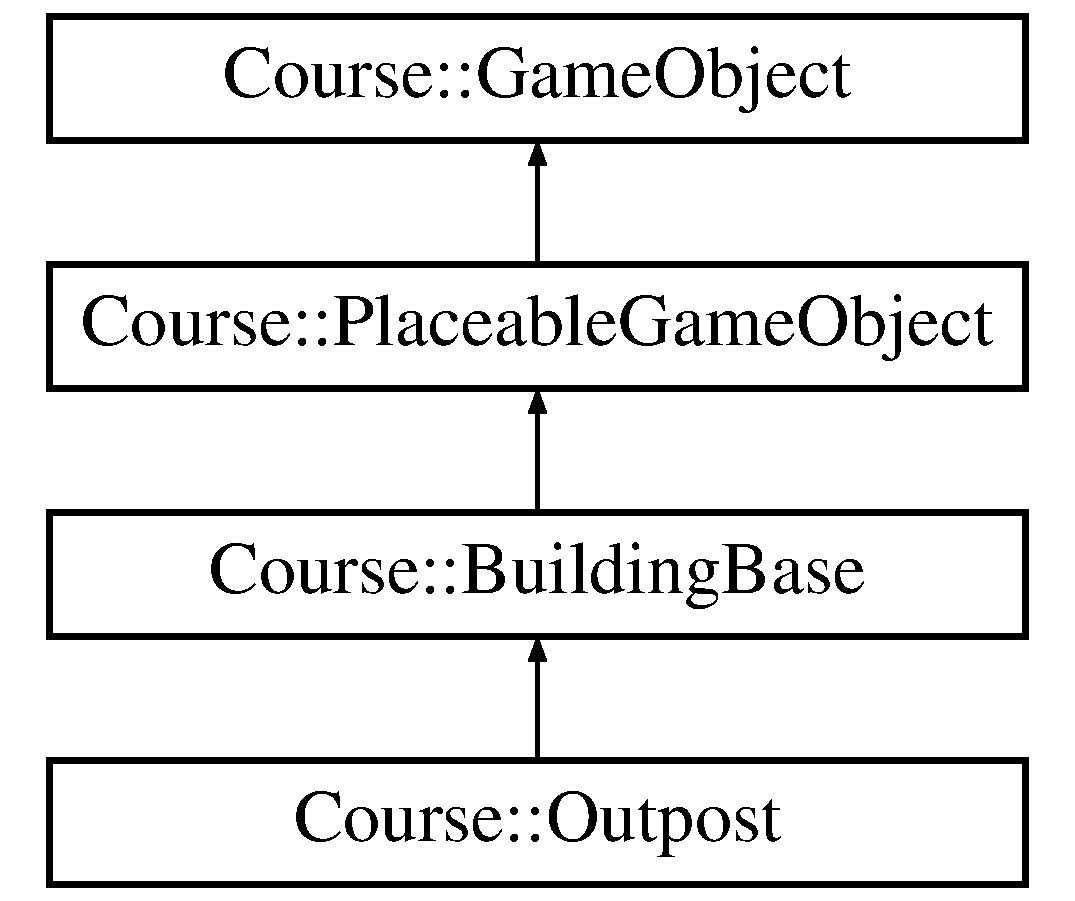
\includegraphics[height=4.000000cm]{classCourse_1_1Outpost}
\end{center}
\end{figure}
\subsection*{Public Member Functions}
\begin{DoxyCompactItemize}
\item 
\hyperlink{classCourse_1_1Outpost_a3b69759306e036223cfd991337c8b4e2}{Outpost} ()=delete
\begin{DoxyCompactList}\small\item\em Disabled parameterless constructor. \end{DoxyCompactList}\item 
\hyperlink{classCourse_1_1Outpost_aa8f768ade225127da85fe4dd9c2c892d}{Outpost} (const std\-::shared\-\_\-ptr$<$ \hyperlink{classCourse_1_1iGameEventHandler}{i\-Game\-Event\-Handler} $>$ \&eventhandler, const std\-::shared\-\_\-ptr$<$ \hyperlink{classCourse_1_1iObjectManager}{i\-Object\-Manager} $>$ \&objectmanager, const std\-::shared\-\_\-ptr$<$ \hyperlink{classCourse_1_1PlayerBase}{Player\-Base} $>$ \&owner, const int \&tilespaces=1, const \hyperlink{namespaceCourse_ab9a46ed9cd00485e318e5731ea2f78d9}{Resource\-Map} \&buildcost=\hyperlink{namespaceCourse_1_1ConstResourceMaps_a0baa840c24b118a34043afeb268c4408}{Const\-Resource\-Maps\-::\-O\-U\-T\-P\-O\-S\-T\-\_\-\-B\-U\-I\-L\-D\-\_\-\-C\-O\-S\-T}, const \hyperlink{namespaceCourse_ab9a46ed9cd00485e318e5731ea2f78d9}{Resource\-Map} \&production=\hyperlink{namespaceCourse_1_1ConstResourceMaps_ae91bf6e7a36ca76016f6d149e94a3e9d}{Const\-Resource\-Maps\-::\-O\-U\-T\-P\-O\-S\-T\-\_\-\-P\-R\-O\-D\-U\-C\-T\-I\-O\-N})
\begin{DoxyCompactList}\small\item\em Constructor for the class. \end{DoxyCompactList}\item 
virtual \hyperlink{classCourse_1_1Outpost_aed6c03ab76797cac0712b1d88660ce14}{$\sim$\-Outpost} ()=default
\begin{DoxyCompactList}\small\item\em Default destructor. \end{DoxyCompactList}\item 
virtual std\-::string \hyperlink{classCourse_1_1Outpost_a8c89c67187451e0a49ecd57d4fc80602}{get\-Type} () const override
\begin{DoxyCompactList}\small\item\em get\-Type Returns a string describing objects type. This should be overriden in each inherited class. Makes checking object's type easier for students. \end{DoxyCompactList}\item 
virtual void \hyperlink{classCourse_1_1Outpost_a81849d7b0b1731051e5f26e9df213d6b}{on\-Build\-Action} () override
\begin{DoxyCompactList}\small\item\em Sets neighbouring Tiles' ownership to this building's ownership in 1 tile-\/radius, if the Tiles don't already have an owner. \end{DoxyCompactList}\item 
virtual \hyperlink{namespaceCourse_ab9a46ed9cd00485e318e5731ea2f78d9}{Resource\-Map} \hyperlink{classCourse_1_1Outpost_a8d27878666500d574e62cea5819c77e2}{get\-Production} () override
\begin{DoxyCompactList}\small\item\em get\-Production \end{DoxyCompactList}\end{DoxyCompactItemize}
\subsection*{Additional Inherited Members}


\subsection{Detailed Description}
The \hyperlink{classCourse_1_1Outpost}{Outpost} class represents a player's Outpost-\/building. 

It can be constructed on any tile that has not been claimed by any other player. \par
Effects\-: Claims surrounding unclaimed tiles. \par
Radius\-: 1 tiles\par
Production\-: -\/10 money (upkeep)\par


\subsection{Constructor \& Destructor Documentation}
\hypertarget{classCourse_1_1Outpost_a3b69759306e036223cfd991337c8b4e2}{\index{Course\-::\-Outpost@{Course\-::\-Outpost}!Outpost@{Outpost}}
\index{Outpost@{Outpost}!Course::Outpost@{Course\-::\-Outpost}}
\subsubsection[{Outpost}]{\setlength{\rightskip}{0pt plus 5cm}Course\-::\-Outpost\-::\-Outpost (
\begin{DoxyParamCaption}
{}
\end{DoxyParamCaption}
)\hspace{0.3cm}{\ttfamily [delete]}}}\label{classCourse_1_1Outpost_a3b69759306e036223cfd991337c8b4e2}


Disabled parameterless constructor. 

\hypertarget{classCourse_1_1Outpost_aa8f768ade225127da85fe4dd9c2c892d}{\index{Course\-::\-Outpost@{Course\-::\-Outpost}!Outpost@{Outpost}}
\index{Outpost@{Outpost}!Course::Outpost@{Course\-::\-Outpost}}
\subsubsection[{Outpost}]{\setlength{\rightskip}{0pt plus 5cm}Course\-::\-Outpost\-::\-Outpost (
\begin{DoxyParamCaption}
\item[{const std\-::shared\-\_\-ptr$<$ {\bf i\-Game\-Event\-Handler} $>$ \&}]{eventhandler, }
\item[{const std\-::shared\-\_\-ptr$<$ {\bf i\-Object\-Manager} $>$ \&}]{objectmanager, }
\item[{const std\-::shared\-\_\-ptr$<$ {\bf Player\-Base} $>$ \&}]{owner, }
\item[{const int \&}]{tilespaces = {\ttfamily 1}, }
\item[{const {\bf Resource\-Map} \&}]{buildcost = {\ttfamily {\bf Const\-Resource\-Maps\-::\-O\-U\-T\-P\-O\-S\-T\-\_\-\-B\-U\-I\-L\-D\-\_\-\-C\-O\-S\-T}}, }
\item[{const {\bf Resource\-Map} \&}]{production = {\ttfamily {\bf Const\-Resource\-Maps\-::\-O\-U\-T\-P\-O\-S\-T\-\_\-\-P\-R\-O\-D\-U\-C\-T\-I\-O\-N}}}
\end{DoxyParamCaption}
)\hspace{0.3cm}{\ttfamily [explicit]}}}\label{classCourse_1_1Outpost_aa8f768ade225127da85fe4dd9c2c892d}


Constructor for the class. 


\begin{DoxyParams}{Parameters}
{\em eventhandler} & points to the student's Game\-Event\-Handler. \\
\hline
{\em owner} & points to the owning player. \\
\hline
{\em tile} & points to the tile upon which the building is constructed.\\
\hline
\end{DoxyParams}
\begin{DoxyPostcond}{Postcondition}
Exception Guarantee\-: No guarantee. 
\end{DoxyPostcond}

\begin{DoxyExceptions}{Exceptions}
{\em \hyperlink{classCourse_1_1OwnerConflict}{Owner\-Conflict}} & -\/ if the building conflicts with tile's ownership. \\
\hline
\end{DoxyExceptions}
\hypertarget{classCourse_1_1Outpost_aed6c03ab76797cac0712b1d88660ce14}{\index{Course\-::\-Outpost@{Course\-::\-Outpost}!$\sim$\-Outpost@{$\sim$\-Outpost}}
\index{$\sim$\-Outpost@{$\sim$\-Outpost}!Course::Outpost@{Course\-::\-Outpost}}
\subsubsection[{$\sim$\-Outpost}]{\setlength{\rightskip}{0pt plus 5cm}virtual Course\-::\-Outpost\-::$\sim$\-Outpost (
\begin{DoxyParamCaption}
{}
\end{DoxyParamCaption}
)\hspace{0.3cm}{\ttfamily [virtual]}, {\ttfamily [default]}}}\label{classCourse_1_1Outpost_aed6c03ab76797cac0712b1d88660ce14}


Default destructor. 



\subsection{Member Function Documentation}
\hypertarget{classCourse_1_1Outpost_a8d27878666500d574e62cea5819c77e2}{\index{Course\-::\-Outpost@{Course\-::\-Outpost}!get\-Production@{get\-Production}}
\index{get\-Production@{get\-Production}!Course::Outpost@{Course\-::\-Outpost}}
\subsubsection[{get\-Production}]{\setlength{\rightskip}{0pt plus 5cm}{\bf Resource\-Map} Course\-::\-Outpost\-::get\-Production (
\begin{DoxyParamCaption}
{}
\end{DoxyParamCaption}
)\hspace{0.3cm}{\ttfamily [override]}, {\ttfamily [virtual]}}}\label{classCourse_1_1Outpost_a8d27878666500d574e62cea5819c77e2}


get\-Production 

\begin{DoxyReturn}{Returns}

\end{DoxyReturn}
\begin{DoxyPostcond}{Postcondition}
Exception guarantee\-: Basic 
\end{DoxyPostcond}


Reimplemented from \hyperlink{classCourse_1_1BuildingBase_ad53ecc1dea91e3ca51c31759fe1680cb}{Course\-::\-Building\-Base}.

\hypertarget{classCourse_1_1Outpost_a8c89c67187451e0a49ecd57d4fc80602}{\index{Course\-::\-Outpost@{Course\-::\-Outpost}!get\-Type@{get\-Type}}
\index{get\-Type@{get\-Type}!Course::Outpost@{Course\-::\-Outpost}}
\subsubsection[{get\-Type}]{\setlength{\rightskip}{0pt plus 5cm}std\-::string Course\-::\-Outpost\-::get\-Type (
\begin{DoxyParamCaption}
{}
\end{DoxyParamCaption}
) const\hspace{0.3cm}{\ttfamily [override]}, {\ttfamily [virtual]}}}\label{classCourse_1_1Outpost_a8c89c67187451e0a49ecd57d4fc80602}


get\-Type Returns a string describing objects type. This should be overriden in each inherited class. Makes checking object's type easier for students. 

\begin{DoxyReturn}{Returns}
std\-::string that represents Object's type. 
\end{DoxyReturn}
\begin{DoxyPostcond}{Postcondition}
Exception guarantee\-: No-\/throw 
\end{DoxyPostcond}
\begin{DoxyNote}{Note}
You can use this in e.\-g. debugging and similar printing. 
\end{DoxyNote}


Reimplemented from \hyperlink{classCourse_1_1BuildingBase_ac2cc44e08dc73d05b1617bf71295baaf}{Course\-::\-Building\-Base}.

\hypertarget{classCourse_1_1Outpost_a81849d7b0b1731051e5f26e9df213d6b}{\index{Course\-::\-Outpost@{Course\-::\-Outpost}!on\-Build\-Action@{on\-Build\-Action}}
\index{on\-Build\-Action@{on\-Build\-Action}!Course::Outpost@{Course\-::\-Outpost}}
\subsubsection[{on\-Build\-Action}]{\setlength{\rightskip}{0pt plus 5cm}void Course\-::\-Outpost\-::on\-Build\-Action (
\begin{DoxyParamCaption}
{}
\end{DoxyParamCaption}
)\hspace{0.3cm}{\ttfamily [override]}, {\ttfamily [virtual]}}}\label{classCourse_1_1Outpost_a81849d7b0b1731051e5f26e9df213d6b}


Sets neighbouring Tiles' ownership to this building's ownership in 1 tile-\/radius, if the Tiles don't already have an owner. 

\begin{DoxyPostcond}{Postcondition}
Exception guarantee\-: Basic 
\end{DoxyPostcond}


Reimplemented from \hyperlink{classCourse_1_1BuildingBase_a2e3a5ad53afb74fdf030a5679e40a341}{Course\-::\-Building\-Base}.



The documentation for this class was generated from the following files\-:\begin{DoxyCompactItemize}
\item 
Course/\-Course\-Lib/buildings/\hyperlink{outpost_8h}{outpost.\-h}\item 
Course/\-Course\-Lib/buildings/\hyperlink{outpost_8cpp}{outpost.\-cpp}\end{DoxyCompactItemize}

\hypertarget{classCourse_1_1OwnerConflict}{\section{Course\-:\-:Owner\-Conflict Class Reference}
\label{classCourse_1_1OwnerConflict}\index{Course\-::\-Owner\-Conflict@{Course\-::\-Owner\-Conflict}}
}


The \hyperlink{classCourse_1_1OwnerConflict}{Owner\-Conflict} class is an Exception-\/class for errors where an operation is conflicting with a \hyperlink{classCourse_1_1GameObject}{Game\-Object}'s ownership.  




{\ttfamily \#include $<$ownerconflict.\-h$>$}

Inheritance diagram for Course\-:\-:Owner\-Conflict\-:\begin{figure}[H]
\begin{center}
\leavevmode
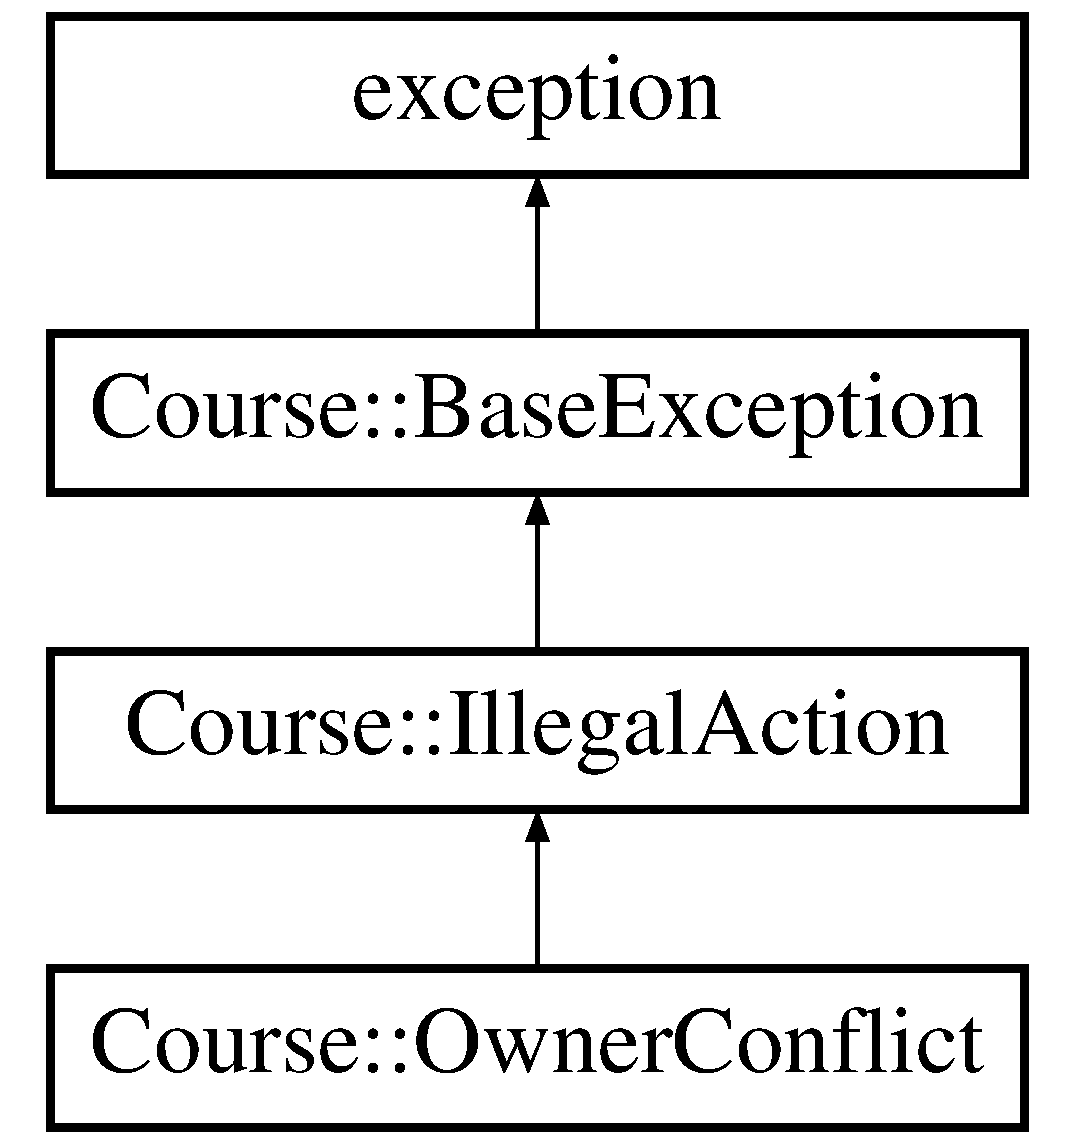
\includegraphics[height=4.000000cm]{classCourse_1_1OwnerConflict}
\end{center}
\end{figure}
\subsection*{Public Member Functions}
\begin{DoxyCompactItemize}
\item 
\hyperlink{classCourse_1_1OwnerConflict_a0f224a172a2cdab0471bc5fc8569c80a}{Owner\-Conflict} (const std\-::string \&\hyperlink{classCourse_1_1BaseException_ac5a744a6af6f2ba9198b58e52bb62f5a}{msg}=\char`\"{}\char`\"{})
\begin{DoxyCompactList}\small\item\em Exception Constructor. \end{DoxyCompactList}\item 
virtual \hyperlink{classCourse_1_1OwnerConflict_a487d89f256b1eb070101affa7ea1b569}{$\sim$\-Owner\-Conflict} ()=default
\begin{DoxyCompactList}\small\item\em $\sim$\-Exception Default destructor \end{DoxyCompactList}\end{DoxyCompactItemize}


\subsection{Detailed Description}
The \hyperlink{classCourse_1_1OwnerConflict}{Owner\-Conflict} class is an Exception-\/class for errors where an operation is conflicting with a \hyperlink{classCourse_1_1GameObject}{Game\-Object}'s ownership. 

\subsection{Constructor \& Destructor Documentation}
\hypertarget{classCourse_1_1OwnerConflict_a0f224a172a2cdab0471bc5fc8569c80a}{\index{Course\-::\-Owner\-Conflict@{Course\-::\-Owner\-Conflict}!Owner\-Conflict@{Owner\-Conflict}}
\index{Owner\-Conflict@{Owner\-Conflict}!Course::OwnerConflict@{Course\-::\-Owner\-Conflict}}
\subsubsection[{Owner\-Conflict}]{\setlength{\rightskip}{0pt plus 5cm}Course\-::\-Owner\-Conflict\-::\-Owner\-Conflict (
\begin{DoxyParamCaption}
\item[{const std\-::string \&}]{msg = {\ttfamily \char`\"{}\char`\"{}}}
\end{DoxyParamCaption}
)\hspace{0.3cm}{\ttfamily [inline]}, {\ttfamily [explicit]}}}\label{classCourse_1_1OwnerConflict_a0f224a172a2cdab0471bc5fc8569c80a}


Exception Constructor. 


\begin{DoxyParams}{Parameters}
{\em msg} & std\-::string describing the reason for exception. \\
\hline
\end{DoxyParams}
\hypertarget{classCourse_1_1OwnerConflict_a487d89f256b1eb070101affa7ea1b569}{\index{Course\-::\-Owner\-Conflict@{Course\-::\-Owner\-Conflict}!$\sim$\-Owner\-Conflict@{$\sim$\-Owner\-Conflict}}
\index{$\sim$\-Owner\-Conflict@{$\sim$\-Owner\-Conflict}!Course::OwnerConflict@{Course\-::\-Owner\-Conflict}}
\subsubsection[{$\sim$\-Owner\-Conflict}]{\setlength{\rightskip}{0pt plus 5cm}virtual Course\-::\-Owner\-Conflict\-::$\sim$\-Owner\-Conflict (
\begin{DoxyParamCaption}
{}
\end{DoxyParamCaption}
)\hspace{0.3cm}{\ttfamily [virtual]}, {\ttfamily [default]}}}\label{classCourse_1_1OwnerConflict_a487d89f256b1eb070101affa7ea1b569}


$\sim$\-Exception Default destructor 



The documentation for this class was generated from the following file\-:\begin{DoxyCompactItemize}
\item 
Course/\-Course\-Lib/exceptions/\hyperlink{ownerconflict_8h}{ownerconflict.\-h}\end{DoxyCompactItemize}

\hypertarget{classCourse_1_1PlaceableGameObject}{\section{Course\-:\-:Placeable\-Game\-Object Class Reference}
\label{classCourse_1_1PlaceableGameObject}\index{Course\-::\-Placeable\-Game\-Object@{Course\-::\-Placeable\-Game\-Object}}
}


The \hyperlink{classCourse_1_1PlaceableGameObject}{Placeable\-Game\-Object} class represents Game\-Objects that can be placed on Tile Objects.  




{\ttfamily \#include $<$placeablegameobject.\-h$>$}

Inheritance diagram for Course\-:\-:Placeable\-Game\-Object\-:\begin{figure}[H]
\begin{center}
\leavevmode
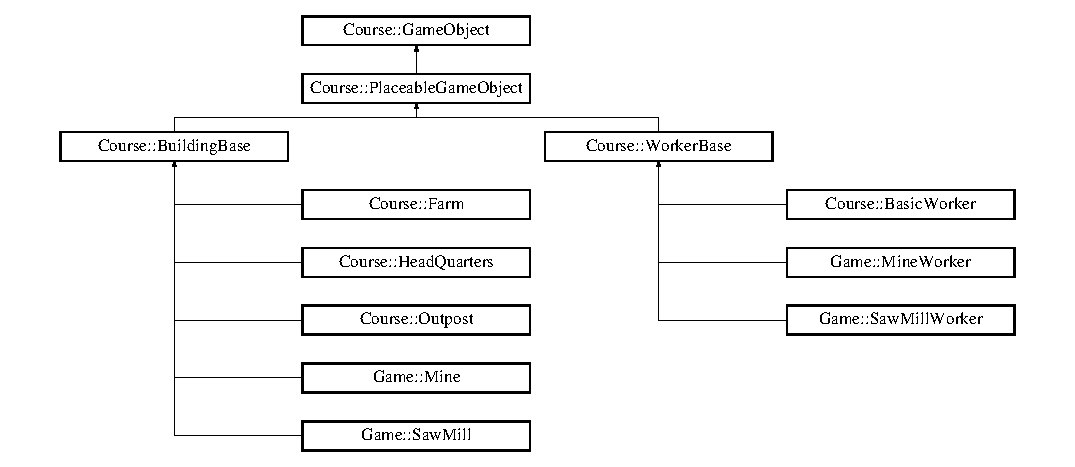
\includegraphics[height=5.833333cm]{classCourse_1_1PlaceableGameObject}
\end{center}
\end{figure}
\subsection*{Public Member Functions}
\begin{DoxyCompactItemize}
\item 
\hyperlink{classCourse_1_1PlaceableGameObject_adde506e2a75757799f54b14b464cf128}{Placeable\-Game\-Object} ()=delete
\begin{DoxyCompactList}\small\item\em Disabled parameterless constructor. \end{DoxyCompactList}\item 
\hyperlink{classCourse_1_1PlaceableGameObject_a021fe249f3a6de1daf8e0a85e772e57e}{Placeable\-Game\-Object} (const std\-::shared\-\_\-ptr$<$ \hyperlink{classCourse_1_1iGameEventHandler}{i\-Game\-Event\-Handler} $>$ \&eventhandler, const std\-::shared\-\_\-ptr$<$ \hyperlink{classCourse_1_1iObjectManager}{i\-Object\-Manager} $>$ \&objectmanager, const std\-::shared\-\_\-ptr$<$ \hyperlink{classCourse_1_1PlayerBase}{Player\-Base} $>$ \&owner, const int \&tilespace=1)
\begin{DoxyCompactList}\small\item\em Constructor for the class. \end{DoxyCompactList}\item 
virtual \hyperlink{classCourse_1_1PlaceableGameObject_ab0e0ad8ecd20bf48faefc6c51056066f}{$\sim$\-Placeable\-Game\-Object} ()=default
\begin{DoxyCompactList}\small\item\em Default destructor. \end{DoxyCompactList}\item 
virtual std\-::string \hyperlink{classCourse_1_1PlaceableGameObject_adcd0c91b52ccedd434092380644f210e}{get\-Type} () const override
\begin{DoxyCompactList}\small\item\em get\-Type Returns a string describing objects type. This should be overriden in each inherited class. Makes checking object's type easier for students. \end{DoxyCompactList}\item 
virtual int \hyperlink{classCourse_1_1PlaceableGameObject_a677e6c0afa7c9cc70123369f3d7dafcb}{spaces\-In\-Tile\-Capacity} () const 
\begin{DoxyCompactList}\small\item\em How many spaces does the \hyperlink{classCourse_1_1GameObject}{Game\-Object} take from a Tile's capacity. \end{DoxyCompactList}\item 
virtual bool \hyperlink{classCourse_1_1PlaceableGameObject_a09616c1b271c35df61c88b37d0b85968}{can\-Be\-Placed\-On\-Tile} (const std\-::shared\-\_\-ptr$<$ \hyperlink{classCourse_1_1TileBase}{Tile\-Base} $>$ \&target) const 
\begin{DoxyCompactList}\small\item\em Check if the object's own placement rules allow placement on the specified tile. \end{DoxyCompactList}\item 
virtual void \hyperlink{classCourse_1_1PlaceableGameObject_a22dcc18962f81c27ac0a176b37533ff4}{set\-Location\-Tile} (const std\-::shared\-\_\-ptr$<$ \hyperlink{classCourse_1_1TileBase}{Tile\-Base} $>$ \&tile) final
\begin{DoxyCompactList}\small\item\em Set the \hyperlink{classCourse_1_1PlaceableGameObject}{Placeable\-Game\-Object}'s location. \end{DoxyCompactList}\item 
virtual std\-::shared\-\_\-ptr$<$ \hyperlink{classCourse_1_1TileBase}{Tile\-Base} $>$ \hyperlink{classCourse_1_1PlaceableGameObject_a860e49fae06b1f58641d9ff373d46fdf}{current\-Location\-Tile} () const final
\begin{DoxyCompactList}\small\item\em Returns a shared\-\_\-ptr to current location-\/tile. \end{DoxyCompactList}\end{DoxyCompactItemize}
\subsection*{Public Attributes}
\begin{DoxyCompactItemize}
\item 
const int \hyperlink{classCourse_1_1PlaceableGameObject_a9f3a7d817d3f90754025fb7a46d7f70d}{T\-I\-L\-E\-S\-P\-A\-C\-E\-S}
\end{DoxyCompactItemize}
\subsection*{Private Attributes}
\begin{DoxyCompactItemize}
\item 
std\-::weak\-\_\-ptr$<$ \hyperlink{classCourse_1_1TileBase}{Tile\-Base} $>$ \hyperlink{classCourse_1_1PlaceableGameObject_a2c59e31d488edddd6cb41e5b39a01456}{m\-\_\-location}
\end{DoxyCompactItemize}
\subsection*{Additional Inherited Members}


\subsection{Detailed Description}
The \hyperlink{classCourse_1_1PlaceableGameObject}{Placeable\-Game\-Object} class represents Game\-Objects that can be placed on Tile Objects. 

Handles placement on a Tile and throws exception if the placement would violate Placeable\-Game\-Objects own placement rules.

\begin{DoxyNote}{Note}
One new overridable method\-: can\-Be\-Placed\-On\-Tile -\/ Can be used to re-\/specify placement-\/rules. 
\end{DoxyNote}


\subsection{Constructor \& Destructor Documentation}
\hypertarget{classCourse_1_1PlaceableGameObject_adde506e2a75757799f54b14b464cf128}{\index{Course\-::\-Placeable\-Game\-Object@{Course\-::\-Placeable\-Game\-Object}!Placeable\-Game\-Object@{Placeable\-Game\-Object}}
\index{Placeable\-Game\-Object@{Placeable\-Game\-Object}!Course::PlaceableGameObject@{Course\-::\-Placeable\-Game\-Object}}
\subsubsection[{Placeable\-Game\-Object}]{\setlength{\rightskip}{0pt plus 5cm}Course\-::\-Placeable\-Game\-Object\-::\-Placeable\-Game\-Object (
\begin{DoxyParamCaption}
{}
\end{DoxyParamCaption}
)\hspace{0.3cm}{\ttfamily [delete]}}}\label{classCourse_1_1PlaceableGameObject_adde506e2a75757799f54b14b464cf128}


Disabled parameterless constructor. 

\hypertarget{classCourse_1_1PlaceableGameObject_a021fe249f3a6de1daf8e0a85e772e57e}{\index{Course\-::\-Placeable\-Game\-Object@{Course\-::\-Placeable\-Game\-Object}!Placeable\-Game\-Object@{Placeable\-Game\-Object}}
\index{Placeable\-Game\-Object@{Placeable\-Game\-Object}!Course::PlaceableGameObject@{Course\-::\-Placeable\-Game\-Object}}
\subsubsection[{Placeable\-Game\-Object}]{\setlength{\rightskip}{0pt plus 5cm}Course\-::\-Placeable\-Game\-Object\-::\-Placeable\-Game\-Object (
\begin{DoxyParamCaption}
\item[{const std\-::shared\-\_\-ptr$<$ {\bf i\-Game\-Event\-Handler} $>$ \&}]{eventhandler, }
\item[{const std\-::shared\-\_\-ptr$<$ {\bf i\-Object\-Manager} $>$ \&}]{objectmanager, }
\item[{const std\-::shared\-\_\-ptr$<$ {\bf Player\-Base} $>$ \&}]{owner, }
\item[{const int \&}]{tilespace = {\ttfamily 1}}
\end{DoxyParamCaption}
)\hspace{0.3cm}{\ttfamily [explicit]}}}\label{classCourse_1_1PlaceableGameObject_a021fe249f3a6de1daf8e0a85e772e57e}


Constructor for the class. 


\begin{DoxyParams}{Parameters}
{\em eventhandler} & points to the student's Game\-Event\-Handler. \\
\hline
{\em objectmanager} & points to the studtent's Object\-Manager \\
\hline
{\em owner} & points to the owning player. \\
\hline
{\em tilespace} & indicates the amount of tilespace the object would take when placed on a tile. \\
\hline
\end{DoxyParams}
\hypertarget{classCourse_1_1PlaceableGameObject_ab0e0ad8ecd20bf48faefc6c51056066f}{\index{Course\-::\-Placeable\-Game\-Object@{Course\-::\-Placeable\-Game\-Object}!$\sim$\-Placeable\-Game\-Object@{$\sim$\-Placeable\-Game\-Object}}
\index{$\sim$\-Placeable\-Game\-Object@{$\sim$\-Placeable\-Game\-Object}!Course::PlaceableGameObject@{Course\-::\-Placeable\-Game\-Object}}
\subsubsection[{$\sim$\-Placeable\-Game\-Object}]{\setlength{\rightskip}{0pt plus 5cm}virtual Course\-::\-Placeable\-Game\-Object\-::$\sim$\-Placeable\-Game\-Object (
\begin{DoxyParamCaption}
{}
\end{DoxyParamCaption}
)\hspace{0.3cm}{\ttfamily [virtual]}, {\ttfamily [default]}}}\label{classCourse_1_1PlaceableGameObject_ab0e0ad8ecd20bf48faefc6c51056066f}


Default destructor. 



\subsection{Member Function Documentation}
\hypertarget{classCourse_1_1PlaceableGameObject_a09616c1b271c35df61c88b37d0b85968}{\index{Course\-::\-Placeable\-Game\-Object@{Course\-::\-Placeable\-Game\-Object}!can\-Be\-Placed\-On\-Tile@{can\-Be\-Placed\-On\-Tile}}
\index{can\-Be\-Placed\-On\-Tile@{can\-Be\-Placed\-On\-Tile}!Course::PlaceableGameObject@{Course\-::\-Placeable\-Game\-Object}}
\subsubsection[{can\-Be\-Placed\-On\-Tile}]{\setlength{\rightskip}{0pt plus 5cm}virtual bool Course\-::\-Placeable\-Game\-Object\-::can\-Be\-Placed\-On\-Tile (
\begin{DoxyParamCaption}
\item[{const std\-::shared\-\_\-ptr$<$ {\bf Tile\-Base} $>$ \&}]{target}
\end{DoxyParamCaption}
) const\hspace{0.3cm}{\ttfamily [virtual]}}}\label{classCourse_1_1PlaceableGameObject_a09616c1b271c35df61c88b37d0b85968}


Check if the object's own placement rules allow placement on the specified tile. 


\begin{DoxyParams}{Parameters}
{\em target} & is a pointer to the tile that is being targeted. \\
\hline
\end{DoxyParams}
\begin{DoxyReturn}{Returns}
\par
True -\/ Object has same owner as the tile.\par
False -\/ If condition doesn't match.\par

\end{DoxyReturn}
\begin{DoxyPostcond}{Postcondition}
Exception guarantee\-: Basic 
\end{DoxyPostcond}
\begin{DoxyNote}{Note}
Override to change default behaviour 
\end{DoxyNote}


Reimplemented in \hyperlink{classCourse_1_1BuildingBase_add23c593f509f39654f2d5abc7d8c072}{Course\-::\-Building\-Base}, \hyperlink{classCourse_1_1WorkerBase_ad80874970ab91bca95b9d3f959e838d2}{Course\-::\-Worker\-Base}, \hyperlink{classGame_1_1MineWorker_aa52833ec99f6746871a78467c51bc57e}{Game\-::\-Mine\-Worker}, \hyperlink{classGame_1_1SawMillWorker_a435e13b35d129a453d7fdfcd60b6dc42}{Game\-::\-Saw\-Mill\-Worker}, and \hyperlink{classCourse_1_1BasicWorker_ab12d85004e92d9a1e85396d72c6cac98}{Course\-::\-Basic\-Worker}.

\hypertarget{classCourse_1_1PlaceableGameObject_a860e49fae06b1f58641d9ff373d46fdf}{\index{Course\-::\-Placeable\-Game\-Object@{Course\-::\-Placeable\-Game\-Object}!current\-Location\-Tile@{current\-Location\-Tile}}
\index{current\-Location\-Tile@{current\-Location\-Tile}!Course::PlaceableGameObject@{Course\-::\-Placeable\-Game\-Object}}
\subsubsection[{current\-Location\-Tile}]{\setlength{\rightskip}{0pt plus 5cm}virtual std\-::shared\-\_\-ptr$<${\bf Tile\-Base}$>$ Course\-::\-Placeable\-Game\-Object\-::current\-Location\-Tile (
\begin{DoxyParamCaption}
{}
\end{DoxyParamCaption}
) const\hspace{0.3cm}{\ttfamily [final]}, {\ttfamily [virtual]}}}\label{classCourse_1_1PlaceableGameObject_a860e49fae06b1f58641d9ff373d46fdf}


Returns a shared\-\_\-ptr to current location-\/tile. 

\begin{DoxyReturn}{Returns}

\end{DoxyReturn}
\begin{DoxyPostcond}{Postcondition}
Exception guarantee\-: No-\/throw 
\end{DoxyPostcond}
\hypertarget{classCourse_1_1PlaceableGameObject_adcd0c91b52ccedd434092380644f210e}{\index{Course\-::\-Placeable\-Game\-Object@{Course\-::\-Placeable\-Game\-Object}!get\-Type@{get\-Type}}
\index{get\-Type@{get\-Type}!Course::PlaceableGameObject@{Course\-::\-Placeable\-Game\-Object}}
\subsubsection[{get\-Type}]{\setlength{\rightskip}{0pt plus 5cm}virtual std\-::string Course\-::\-Placeable\-Game\-Object\-::get\-Type (
\begin{DoxyParamCaption}
{}
\end{DoxyParamCaption}
) const\hspace{0.3cm}{\ttfamily [override]}, {\ttfamily [virtual]}}}\label{classCourse_1_1PlaceableGameObject_adcd0c91b52ccedd434092380644f210e}


get\-Type Returns a string describing objects type. This should be overriden in each inherited class. Makes checking object's type easier for students. 

\begin{DoxyReturn}{Returns}
std\-::string that represents Object's type. 
\end{DoxyReturn}
\begin{DoxyPostcond}{Postcondition}
Exception guarantee\-: No-\/throw 
\end{DoxyPostcond}
\begin{DoxyNote}{Note}
You can use this in e.\-g. debugging and similar printing. 
\end{DoxyNote}


Reimplemented from \hyperlink{classCourse_1_1GameObject_aeecb0b8f5ed8d7b379e0e38ef4ebba10}{Course\-::\-Game\-Object}.



Reimplemented in \hyperlink{classCourse_1_1WorkerBase_afe6049810eec47fffe2c2a7334564ef9}{Course\-::\-Worker\-Base}, \hyperlink{classCourse_1_1BuildingBase_ac2cc44e08dc73d05b1617bf71295baaf}{Course\-::\-Building\-Base}, \hyperlink{classCourse_1_1Outpost_a8c89c67187451e0a49ecd57d4fc80602}{Course\-::\-Outpost}, \hyperlink{classGame_1_1MineWorker_a984c2ede11ac50460620a4d982249dbe}{Game\-::\-Mine\-Worker}, \hyperlink{classGame_1_1SawMillWorker_af64ec6de521d31ec3fdc885a3bc69cba}{Game\-::\-Saw\-Mill\-Worker}, \hyperlink{classCourse_1_1BasicWorker_a8396e00dafd128cbb86e479296d75c12}{Course\-::\-Basic\-Worker}, \hyperlink{classCourse_1_1HeadQuarters_a1d9a996a6a87ca31aeb63dff2d41d242}{Course\-::\-Head\-Quarters}, \hyperlink{classGame_1_1Mine_aaf18e426d1978c8e6f0cf0dc7435c257}{Game\-::\-Mine}, \hyperlink{classGame_1_1SawMill_a1dd6fd6bce2044107b121f3bbf012691}{Game\-::\-Saw\-Mill}, and \hyperlink{classCourse_1_1Farm_a54ade72809a36d31e0e426eb79d6251a}{Course\-::\-Farm}.

\hypertarget{classCourse_1_1PlaceableGameObject_a22dcc18962f81c27ac0a176b37533ff4}{\index{Course\-::\-Placeable\-Game\-Object@{Course\-::\-Placeable\-Game\-Object}!set\-Location\-Tile@{set\-Location\-Tile}}
\index{set\-Location\-Tile@{set\-Location\-Tile}!Course::PlaceableGameObject@{Course\-::\-Placeable\-Game\-Object}}
\subsubsection[{set\-Location\-Tile}]{\setlength{\rightskip}{0pt plus 5cm}virtual void Course\-::\-Placeable\-Game\-Object\-::set\-Location\-Tile (
\begin{DoxyParamCaption}
\item[{const std\-::shared\-\_\-ptr$<$ {\bf Tile\-Base} $>$ \&}]{tile}
\end{DoxyParamCaption}
)\hspace{0.3cm}{\ttfamily [final]}, {\ttfamily [virtual]}}}\label{classCourse_1_1PlaceableGameObject_a22dcc18962f81c27ac0a176b37533ff4}


Set the \hyperlink{classCourse_1_1PlaceableGameObject}{Placeable\-Game\-Object}'s location. 


\begin{DoxyParams}{Parameters}
{\em tile} & points to the Tile where the object is placed. \\
\hline
\end{DoxyParams}
\begin{DoxyPostcond}{Postcondition}
Exception guarantee\-: Strong 
\end{DoxyPostcond}
\begin{DoxyNote}{Note}
nullptr can be used to clear the location. 
\end{DoxyNote}

\begin{DoxyExceptions}{Exceptions}
{\em \hyperlink{classCourse_1_1IllegalAction}{Illegal\-Action}} & -\/ If can\-Be\-Placed\-On\-Tile returns False. \\
\hline
\end{DoxyExceptions}
\hypertarget{classCourse_1_1PlaceableGameObject_a677e6c0afa7c9cc70123369f3d7dafcb}{\index{Course\-::\-Placeable\-Game\-Object@{Course\-::\-Placeable\-Game\-Object}!spaces\-In\-Tile\-Capacity@{spaces\-In\-Tile\-Capacity}}
\index{spaces\-In\-Tile\-Capacity@{spaces\-In\-Tile\-Capacity}!Course::PlaceableGameObject@{Course\-::\-Placeable\-Game\-Object}}
\subsubsection[{spaces\-In\-Tile\-Capacity}]{\setlength{\rightskip}{0pt plus 5cm}virtual int Course\-::\-Placeable\-Game\-Object\-::spaces\-In\-Tile\-Capacity (
\begin{DoxyParamCaption}
{}
\end{DoxyParamCaption}
) const\hspace{0.3cm}{\ttfamily [virtual]}}}\label{classCourse_1_1PlaceableGameObject_a677e6c0afa7c9cc70123369f3d7dafcb}


How many spaces does the \hyperlink{classCourse_1_1GameObject}{Game\-Object} take from a Tile's capacity. 

\begin{DoxyReturn}{Returns}
Amount of spaces that is being taken. 
\end{DoxyReturn}
\begin{DoxyPostcond}{Postcondition}
Exception guarantee\-: No-\/throw 
\end{DoxyPostcond}


\subsection{Member Data Documentation}
\hypertarget{classCourse_1_1PlaceableGameObject_a2c59e31d488edddd6cb41e5b39a01456}{\index{Course\-::\-Placeable\-Game\-Object@{Course\-::\-Placeable\-Game\-Object}!m\-\_\-location@{m\-\_\-location}}
\index{m\-\_\-location@{m\-\_\-location}!Course::PlaceableGameObject@{Course\-::\-Placeable\-Game\-Object}}
\subsubsection[{m\-\_\-location}]{\setlength{\rightskip}{0pt plus 5cm}std\-::weak\-\_\-ptr$<${\bf Tile\-Base}$>$ Course\-::\-Placeable\-Game\-Object\-::m\-\_\-location\hspace{0.3cm}{\ttfamily [private]}}}\label{classCourse_1_1PlaceableGameObject_a2c59e31d488edddd6cb41e5b39a01456}
\hypertarget{classCourse_1_1PlaceableGameObject_a9f3a7d817d3f90754025fb7a46d7f70d}{\index{Course\-::\-Placeable\-Game\-Object@{Course\-::\-Placeable\-Game\-Object}!T\-I\-L\-E\-S\-P\-A\-C\-E\-S@{T\-I\-L\-E\-S\-P\-A\-C\-E\-S}}
\index{T\-I\-L\-E\-S\-P\-A\-C\-E\-S@{T\-I\-L\-E\-S\-P\-A\-C\-E\-S}!Course::PlaceableGameObject@{Course\-::\-Placeable\-Game\-Object}}
\subsubsection[{T\-I\-L\-E\-S\-P\-A\-C\-E\-S}]{\setlength{\rightskip}{0pt plus 5cm}const int Course\-::\-Placeable\-Game\-Object\-::\-T\-I\-L\-E\-S\-P\-A\-C\-E\-S}}\label{classCourse_1_1PlaceableGameObject_a9f3a7d817d3f90754025fb7a46d7f70d}


The documentation for this class was generated from the following files\-:\begin{DoxyCompactItemize}
\item 
Course/\-Course\-Lib/core/\hyperlink{placeablegameobject_8h}{placeablegameobject.\-h}\item 
Course/\-Course\-Lib/core/\hyperlink{placeablegameobject_8cpp}{placeablegameobject.\-cpp}\end{DoxyCompactItemize}

\hypertarget{classGame_1_1Player}{\section{Game\-:\-:Player Class Reference}
\label{classGame_1_1Player}\index{Game\-::\-Player@{Game\-::\-Player}}
}


The \hyperlink{classGame_1_1Player}{Player} class represents a player in the game.  




{\ttfamily \#include $<$player.\-h$>$}

Inheritance diagram for Game\-:\-:Player\-:\begin{figure}[H]
\begin{center}
\leavevmode
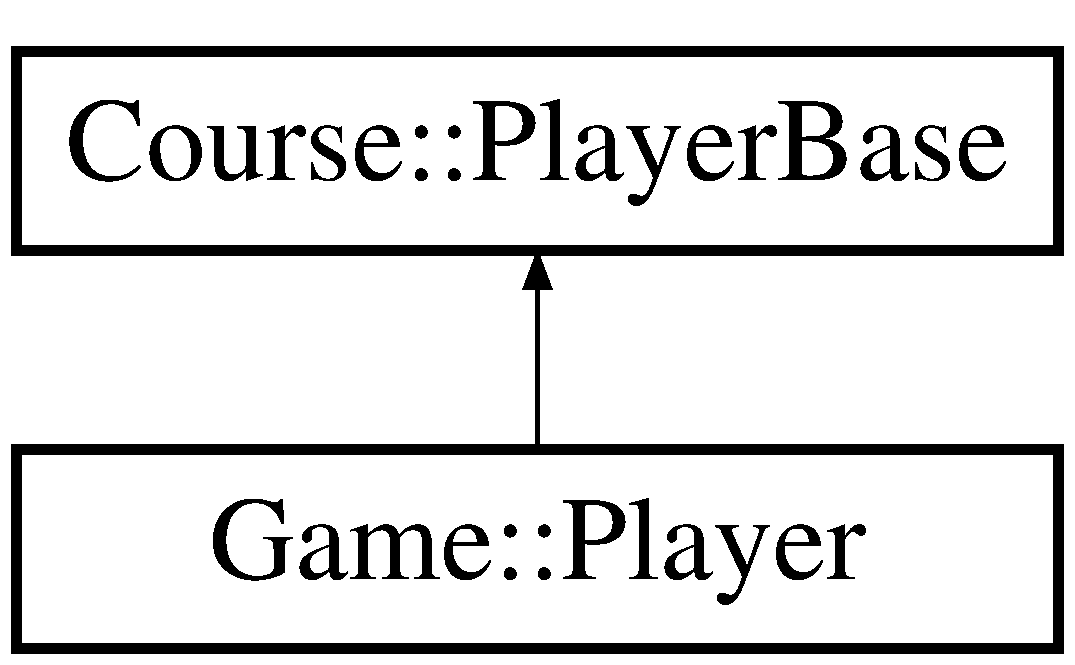
\includegraphics[height=2.000000cm]{classGame_1_1Player}
\end{center}
\end{figure}
\subsection*{Public Member Functions}
\begin{DoxyCompactItemize}
\item 
\hyperlink{classGame_1_1Player_a1550c6bbc0e31a91847fd1bfa61ebbd5}{Player} (const std\-::string \&name, Q\-String color, const std\-::vector$<$ std\-::shared\-\_\-ptr$<$ \hyperlink{classCourse_1_1GameObject}{Course\-::\-Game\-Object} $>$ $>$ objects=\{\})
\begin{DoxyCompactList}\small\item\em Constructor for the class. \end{DoxyCompactList}\item 
bool \hyperlink{classGame_1_1Player_aec9c6bb5b0ee04271f84a99d90663d7f}{modify\-Resource} (const \hyperlink{namespaceCourse_a02d49c04029594d4adba79b84bb85f65}{Course\-::\-Basic\-Resource} \&resource, const int \&amount)
\begin{DoxyCompactList}\small\item\em Modifies a players resource (by addition) \end{DoxyCompactList}\item 
bool \hyperlink{classGame_1_1Player_a68980b4a5e45acca17bfeb6674031526}{modify\-Resources} (const \hyperlink{namespaceCourse_ab9a46ed9cd00485e318e5731ea2f78d9}{Course\-::\-Resource\-Map} \&resources)
\begin{DoxyCompactList}\small\item\em Modifies a players resources (by addition) \end{DoxyCompactList}\item 
\hyperlink{namespaceCourse_ab9a46ed9cd00485e318e5731ea2f78d9}{Course\-::\-Resource\-Map} \hyperlink{classGame_1_1Player_a3614aac3989870a566469c9df26f8a19}{get\-Resources} () const 
\begin{DoxyCompactList}\small\item\em Returns the player's resources. \end{DoxyCompactList}\item 
const Q\-String \hyperlink{classGame_1_1Player_a60dafb9daab8ce844f69cc0d78dabd5a}{get\-Color} () const 
\begin{DoxyCompactList}\small\item\em Returns the player's color. \end{DoxyCompactList}\end{DoxyCompactItemize}
\subsection*{Private Attributes}
\begin{DoxyCompactItemize}
\item 
\hyperlink{namespaceCourse_ab9a46ed9cd00485e318e5731ea2f78d9}{Course\-::\-Resource\-Map} \hyperlink{classGame_1_1Player_a78e032ef0212488e590267e4bd101400}{m\-\_\-resources}
\item 
Q\-String \hyperlink{classGame_1_1Player_aba8134395ff2502baa9dddbd4ebea5ad}{m\-\_\-color}
\end{DoxyCompactItemize}


\subsection{Detailed Description}
The \hyperlink{classGame_1_1Player}{Player} class represents a player in the game. 

\hyperlink{classGame_1_1Player}{Player} has a name, color and ownership to Game\-Objects 

\subsection{Constructor \& Destructor Documentation}
\hypertarget{classGame_1_1Player_a1550c6bbc0e31a91847fd1bfa61ebbd5}{\index{Game\-::\-Player@{Game\-::\-Player}!Player@{Player}}
\index{Player@{Player}!Game::Player@{Game\-::\-Player}}
\subsubsection[{Player}]{\setlength{\rightskip}{0pt plus 5cm}Game\-::\-Player\-::\-Player (
\begin{DoxyParamCaption}
\item[{const std\-::string \&}]{name, }
\item[{Q\-String}]{color, }
\item[{const std\-::vector$<$ std\-::shared\-\_\-ptr$<$ {\bf Course\-::\-Game\-Object} $>$ $>$}]{objects = {\ttfamily \{\}}}
\end{DoxyParamCaption}
)}}\label{classGame_1_1Player_a1550c6bbc0e31a91847fd1bfa61ebbd5}


Constructor for the class. 


\begin{DoxyParams}{Parameters}
{\em name} & A std\-::string for player's name \\
\hline
{\em color} & \hyperlink{classGame_1_1Player}{Player}'s color in the game as a string \\
\hline
{\em objects} & (optional) A std\-::vector of shared-\/pointers to Game\-Objects. \\
\hline
\end{DoxyParams}


\subsection{Member Function Documentation}
\hypertarget{classGame_1_1Player_a60dafb9daab8ce844f69cc0d78dabd5a}{\index{Game\-::\-Player@{Game\-::\-Player}!get\-Color@{get\-Color}}
\index{get\-Color@{get\-Color}!Game::Player@{Game\-::\-Player}}
\subsubsection[{get\-Color}]{\setlength{\rightskip}{0pt plus 5cm}const Q\-String Game\-::\-Player\-::get\-Color (
\begin{DoxyParamCaption}
{}
\end{DoxyParamCaption}
) const}}\label{classGame_1_1Player_a60dafb9daab8ce844f69cc0d78dabd5a}


Returns the player's color. 

\begin{DoxyReturn}{Returns}
Qstring that tells the player's color 
\end{DoxyReturn}
\hypertarget{classGame_1_1Player_a3614aac3989870a566469c9df26f8a19}{\index{Game\-::\-Player@{Game\-::\-Player}!get\-Resources@{get\-Resources}}
\index{get\-Resources@{get\-Resources}!Game::Player@{Game\-::\-Player}}
\subsubsection[{get\-Resources}]{\setlength{\rightskip}{0pt plus 5cm}{\bf Course\-::\-Resource\-Map} Game\-::\-Player\-::get\-Resources (
\begin{DoxyParamCaption}
{}
\end{DoxyParamCaption}
) const}}\label{classGame_1_1Player_a3614aac3989870a566469c9df26f8a19}


Returns the player's resources. 

\begin{DoxyReturn}{Returns}
Resource\-Map containing players resources 
\end{DoxyReturn}
\hypertarget{classGame_1_1Player_aec9c6bb5b0ee04271f84a99d90663d7f}{\index{Game\-::\-Player@{Game\-::\-Player}!modify\-Resource@{modify\-Resource}}
\index{modify\-Resource@{modify\-Resource}!Game::Player@{Game\-::\-Player}}
\subsubsection[{modify\-Resource}]{\setlength{\rightskip}{0pt plus 5cm}bool Game\-::\-Player\-::modify\-Resource (
\begin{DoxyParamCaption}
\item[{const {\bf Course\-::\-Basic\-Resource} \&}]{resource, }
\item[{const int \&}]{amount}
\end{DoxyParamCaption}
)}}\label{classGame_1_1Player_aec9c6bb5b0ee04271f84a99d90663d7f}


Modifies a players resource (by addition) 


\begin{DoxyParams}{Parameters}
{\em resource} & A Basic\-Resource type that is modified \\
\hline
{\em amount} & Amount of that resource \\
\hline
\end{DoxyParams}
\begin{DoxyReturn}{Returns}
Bool that tells if the operation was successful 
\end{DoxyReturn}
\hypertarget{classGame_1_1Player_a68980b4a5e45acca17bfeb6674031526}{\index{Game\-::\-Player@{Game\-::\-Player}!modify\-Resources@{modify\-Resources}}
\index{modify\-Resources@{modify\-Resources}!Game::Player@{Game\-::\-Player}}
\subsubsection[{modify\-Resources}]{\setlength{\rightskip}{0pt plus 5cm}bool Game\-::\-Player\-::modify\-Resources (
\begin{DoxyParamCaption}
\item[{const {\bf Course\-::\-Resource\-Map} \&}]{resources}
\end{DoxyParamCaption}
)}}\label{classGame_1_1Player_a68980b4a5e45acca17bfeb6674031526}


Modifies a players resources (by addition) 


\begin{DoxyParams}{Parameters}
{\em resources} & A Resource\-Map that is added to players resources \\
\hline
\end{DoxyParams}
\begin{DoxyReturn}{Returns}
Bool that tells if the operation was successful 
\end{DoxyReturn}


\subsection{Member Data Documentation}
\hypertarget{classGame_1_1Player_aba8134395ff2502baa9dddbd4ebea5ad}{\index{Game\-::\-Player@{Game\-::\-Player}!m\-\_\-color@{m\-\_\-color}}
\index{m\-\_\-color@{m\-\_\-color}!Game::Player@{Game\-::\-Player}}
\subsubsection[{m\-\_\-color}]{\setlength{\rightskip}{0pt plus 5cm}Q\-String Game\-::\-Player\-::m\-\_\-color\hspace{0.3cm}{\ttfamily [private]}}}\label{classGame_1_1Player_aba8134395ff2502baa9dddbd4ebea5ad}
\hypertarget{classGame_1_1Player_a78e032ef0212488e590267e4bd101400}{\index{Game\-::\-Player@{Game\-::\-Player}!m\-\_\-resources@{m\-\_\-resources}}
\index{m\-\_\-resources@{m\-\_\-resources}!Game::Player@{Game\-::\-Player}}
\subsubsection[{m\-\_\-resources}]{\setlength{\rightskip}{0pt plus 5cm}{\bf Course\-::\-Resource\-Map} Game\-::\-Player\-::m\-\_\-resources\hspace{0.3cm}{\ttfamily [private]}}}\label{classGame_1_1Player_a78e032ef0212488e590267e4bd101400}


The documentation for this class was generated from the following files\-:\begin{DoxyCompactItemize}
\item 
Game/core/\hyperlink{player_8h}{player.\-h}\item 
Game/core/\hyperlink{player_8cpp}{player.\-cpp}\end{DoxyCompactItemize}

\hypertarget{classCourse_1_1PlayerBase}{\section{Course\-:\-:Player\-Base Class Reference}
\label{classCourse_1_1PlayerBase}\index{Course\-::\-Player\-Base@{Course\-::\-Player\-Base}}
}


The \hyperlink{classCourse_1_1PlayerBase}{Player\-Base} class is a base class for classes used to describe a player in game.  




{\ttfamily \#include $<$playerbase.\-h$>$}

Inheritance diagram for Course\-:\-:Player\-Base\-:\begin{figure}[H]
\begin{center}
\leavevmode
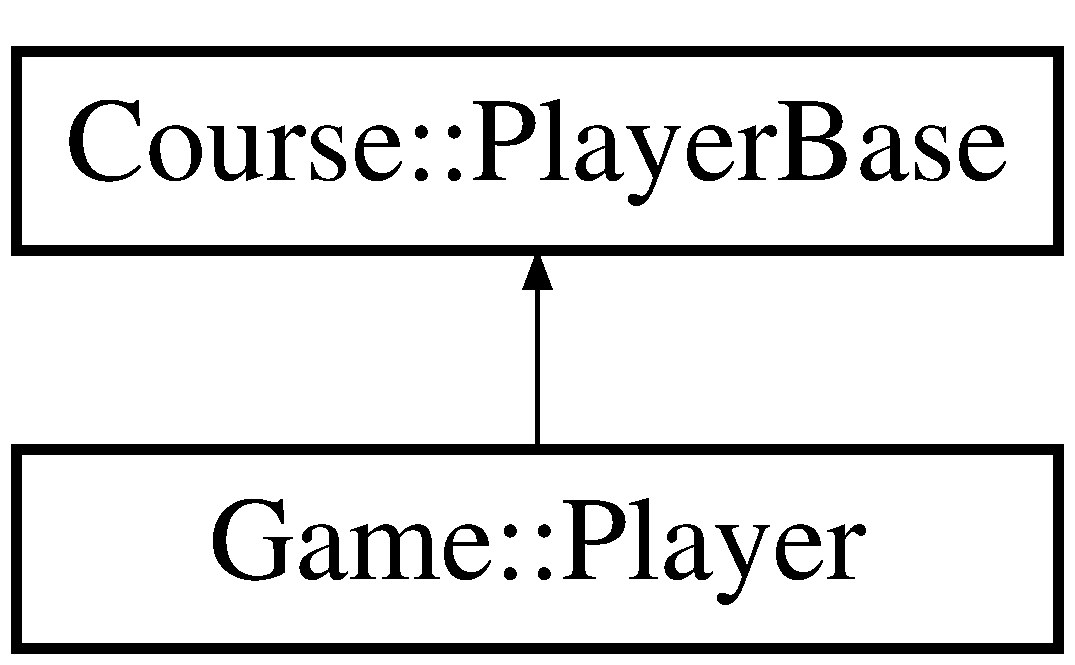
\includegraphics[height=2.000000cm]{classCourse_1_1PlayerBase}
\end{center}
\end{figure}
\subsection*{Public Member Functions}
\begin{DoxyCompactItemize}
\item 
\hyperlink{classCourse_1_1PlayerBase_a6a0c8d316a63aedd52b8de7e19a1ca58}{Player\-Base} (const std\-::string \&name, const std\-::vector$<$ std\-::shared\-\_\-ptr$<$ \hyperlink{classCourse_1_1GameObject}{Game\-Object} $>$ $>$ objects=\{\})
\begin{DoxyCompactList}\small\item\em Constructor for the class. \end{DoxyCompactList}\item 
virtual \hyperlink{classCourse_1_1PlayerBase_a03a96c594802234264f687f981a4d1e7}{$\sim$\-Player\-Base} ()=default
\begin{DoxyCompactList}\small\item\em Default destructor. \end{DoxyCompactList}\item 
virtual void \hyperlink{classCourse_1_1PlayerBase_a15433e03022021d7ea002f3283be5de8}{set\-Name} (const std\-::string \&new\-\_\-name) final
\begin{DoxyCompactList}\small\item\em Sets a new m\-\_\-name value for the class. \end{DoxyCompactList}\item 
virtual void \hyperlink{classCourse_1_1PlayerBase_afc810bbdf7f879458ac125cc06e462d9}{add\-Object} (std\-::shared\-\_\-ptr$<$ \hyperlink{classCourse_1_1GameObject}{Game\-Object} $>$ object) final
\begin{DoxyCompactList}\small\item\em Stores a weak Game\-Object-\/pointer. \end{DoxyCompactList}\item 
virtual void \hyperlink{classCourse_1_1PlayerBase_a01e8c70b87440b2b9229bb3a779e599c}{add\-Objects} (const std\-::vector$<$ std\-::shared\-\_\-ptr$<$ \hyperlink{classCourse_1_1GameObject}{Game\-Object} $>$ $>$ \&objects) final
\begin{DoxyCompactList}\small\item\em Stores a vector of weak Game\-Object-\/pointers. \end{DoxyCompactList}\item 
virtual void \hyperlink{classCourse_1_1PlayerBase_a1d3ccf57f7d582db179d2f63504a2f79}{remove\-Object} (const std\-::shared\-\_\-ptr$<$ \hyperlink{classCourse_1_1GameObject}{Game\-Object} $>$ \&object) final
\begin{DoxyCompactList}\small\item\em Removes a weak Game\-Object-\/pointer and expired weak pointers. \end{DoxyCompactList}\item 
virtual void \hyperlink{classCourse_1_1PlayerBase_a1ec03fd654d82d9924f77c1a29b80569}{remove\-Objects} (const std\-::vector$<$ std\-::shared\-\_\-ptr$<$ \hyperlink{classCourse_1_1GameObject}{Game\-Object} $>$ $>$ \&objects) final
\begin{DoxyCompactList}\small\item\em Removes a list of weak Game\-Object-\/pointers and expired weak pointers. \end{DoxyCompactList}\item 
virtual void \hyperlink{classCourse_1_1PlayerBase_a98b6f65f5162a34906956852b6382201}{remove\-Object} (const \hyperlink{namespaceCourse_a9a16e743c9813da00109e4991afd2f3e}{Object\-Id} \&id) final
\begin{DoxyCompactList}\small\item\em Removes a weak Game\-Object-\/pointers based on a Object\-Id and removes expired weak pointers. \end{DoxyCompactList}\item 
virtual void \hyperlink{classCourse_1_1PlayerBase_a994b8e326315ed80f18482b32b0d8f3d}{remove\-Objects} (const std\-::vector$<$ \hyperlink{namespaceCourse_a9a16e743c9813da00109e4991afd2f3e}{Object\-Id} $>$ \&objects) final
\begin{DoxyCompactList}\small\item\em Removes a list of weak Game\-Object-\/pointers based on a Object\-Id and removes expired weak pointers. \end{DoxyCompactList}\item 
virtual std\-::vector\\*
$<$ std\-::shared\-\_\-ptr$<$ \hyperlink{classCourse_1_1GameObject}{Game\-Object} $>$ $>$ \hyperlink{classCourse_1_1PlayerBase_ad7ab46149c53b6b8b01a43e721ad11b9}{get\-Objects} () const final
\begin{DoxyCompactList}\small\item\em Returns the vector of weak Game\-Object-\/pointers that are currently stored in the Player-\/object. \end{DoxyCompactList}\item 
virtual std\-::string \hyperlink{classCourse_1_1PlayerBase_ac942dc579051e53d261f60196fd35fee}{get\-Name} () const final
\begin{DoxyCompactList}\small\item\em Returns the Player-\/object's name. \end{DoxyCompactList}\end{DoxyCompactItemize}
\subsection*{Private Attributes}
\begin{DoxyCompactItemize}
\item 
std\-::string \hyperlink{classCourse_1_1PlayerBase_a9150ef79abdb0ccca8da46c1e51af28e}{m\-\_\-name}
\item 
std\-::vector$<$ std\-::weak\-\_\-ptr\\*
$<$ \hyperlink{classCourse_1_1GameObject}{Game\-Object} $>$ $>$ \hyperlink{classCourse_1_1PlayerBase_a448c91866b245f8bb3a011835dde19af}{m\-\_\-objects}
\end{DoxyCompactItemize}


\subsection{Detailed Description}
The \hyperlink{classCourse_1_1PlayerBase}{Player\-Base} class is a base class for classes used to describe a player in game. 

The class can be used to store and access Game\-Objects. Expired weak pointers are automatically removed when requesting or removing objects.

\begin{DoxyNote}{Note}
Objects are stored as weak pointers. 
\end{DoxyNote}


\subsection{Constructor \& Destructor Documentation}
\hypertarget{classCourse_1_1PlayerBase_a6a0c8d316a63aedd52b8de7e19a1ca58}{\index{Course\-::\-Player\-Base@{Course\-::\-Player\-Base}!Player\-Base@{Player\-Base}}
\index{Player\-Base@{Player\-Base}!Course::PlayerBase@{Course\-::\-Player\-Base}}
\subsubsection[{Player\-Base}]{\setlength{\rightskip}{0pt plus 5cm}Course\-::\-Player\-Base\-::\-Player\-Base (
\begin{DoxyParamCaption}
\item[{const std\-::string \&}]{name, }
\item[{const std\-::vector$<$ std\-::shared\-\_\-ptr$<$ {\bf Game\-Object} $>$ $>$}]{objects = {\ttfamily \{\}}}
\end{DoxyParamCaption}
)}}\label{classCourse_1_1PlayerBase_a6a0c8d316a63aedd52b8de7e19a1ca58}


Constructor for the class. 


\begin{DoxyParams}{Parameters}
{\em name} & A std\-::string for player's name \\
\hline
{\em objects} & (optional) A std\-::vector of shared-\/pointers to Game\-Objects. \\
\hline
\end{DoxyParams}
\hypertarget{classCourse_1_1PlayerBase_a03a96c594802234264f687f981a4d1e7}{\index{Course\-::\-Player\-Base@{Course\-::\-Player\-Base}!$\sim$\-Player\-Base@{$\sim$\-Player\-Base}}
\index{$\sim$\-Player\-Base@{$\sim$\-Player\-Base}!Course::PlayerBase@{Course\-::\-Player\-Base}}
\subsubsection[{$\sim$\-Player\-Base}]{\setlength{\rightskip}{0pt plus 5cm}virtual Course\-::\-Player\-Base\-::$\sim$\-Player\-Base (
\begin{DoxyParamCaption}
{}
\end{DoxyParamCaption}
)\hspace{0.3cm}{\ttfamily [virtual]}, {\ttfamily [default]}}}\label{classCourse_1_1PlayerBase_a03a96c594802234264f687f981a4d1e7}


Default destructor. 



\subsection{Member Function Documentation}
\hypertarget{classCourse_1_1PlayerBase_afc810bbdf7f879458ac125cc06e462d9}{\index{Course\-::\-Player\-Base@{Course\-::\-Player\-Base}!add\-Object@{add\-Object}}
\index{add\-Object@{add\-Object}!Course::PlayerBase@{Course\-::\-Player\-Base}}
\subsubsection[{add\-Object}]{\setlength{\rightskip}{0pt plus 5cm}void Course\-::\-Player\-Base\-::add\-Object (
\begin{DoxyParamCaption}
\item[{std\-::shared\-\_\-ptr$<$ {\bf Game\-Object} $>$}]{object}
\end{DoxyParamCaption}
)\hspace{0.3cm}{\ttfamily [final]}, {\ttfamily [virtual]}}}\label{classCourse_1_1PlayerBase_afc810bbdf7f879458ac125cc06e462d9}


Stores a weak Game\-Object-\/pointer. 


\begin{DoxyParams}{Parameters}
{\em object} & Is a weak pointer to the stored \hyperlink{classCourse_1_1GameObject}{Game\-Object} \\
\hline
\end{DoxyParams}
\begin{DoxyPostcond}{Postcondition}
Exception guarantee\-: Strong 
\end{DoxyPostcond}

\begin{DoxyExceptions}{Exceptions}
{\em See} & std\-::vector\-::push\-\_\-back() \\
\hline
\end{DoxyExceptions}
\hypertarget{classCourse_1_1PlayerBase_a01e8c70b87440b2b9229bb3a779e599c}{\index{Course\-::\-Player\-Base@{Course\-::\-Player\-Base}!add\-Objects@{add\-Objects}}
\index{add\-Objects@{add\-Objects}!Course::PlayerBase@{Course\-::\-Player\-Base}}
\subsubsection[{add\-Objects}]{\setlength{\rightskip}{0pt plus 5cm}void Course\-::\-Player\-Base\-::add\-Objects (
\begin{DoxyParamCaption}
\item[{const std\-::vector$<$ std\-::shared\-\_\-ptr$<$ {\bf Game\-Object} $>$ $>$ \&}]{objects}
\end{DoxyParamCaption}
)\hspace{0.3cm}{\ttfamily [final]}, {\ttfamily [virtual]}}}\label{classCourse_1_1PlayerBase_a01e8c70b87440b2b9229bb3a779e599c}


Stores a vector of weak Game\-Object-\/pointers. 


\begin{DoxyParams}{Parameters}
{\em objects} & Is an std\-::vector of weak Game\-Object-\/pointers. \\
\hline
\end{DoxyParams}
\begin{DoxyPostcond}{Postcondition}
Exception guarantee\-: Strong 
\end{DoxyPostcond}

\begin{DoxyExceptions}{Exceptions}
{\em See} & std\-::vector\-::insert() \\
\hline
\end{DoxyExceptions}
\hypertarget{classCourse_1_1PlayerBase_ac942dc579051e53d261f60196fd35fee}{\index{Course\-::\-Player\-Base@{Course\-::\-Player\-Base}!get\-Name@{get\-Name}}
\index{get\-Name@{get\-Name}!Course::PlayerBase@{Course\-::\-Player\-Base}}
\subsubsection[{get\-Name}]{\setlength{\rightskip}{0pt plus 5cm}std\-::string Course\-::\-Player\-Base\-::get\-Name (
\begin{DoxyParamCaption}
{}
\end{DoxyParamCaption}
) const\hspace{0.3cm}{\ttfamily [final]}, {\ttfamily [virtual]}}}\label{classCourse_1_1PlayerBase_ac942dc579051e53d261f60196fd35fee}


Returns the Player-\/object's name. 

\begin{DoxyReturn}{Returns}
Copy of current string in m\-\_\-name 
\end{DoxyReturn}
\begin{DoxyPostcond}{Postcondition}
Exception guarantee\-: No-\/throw 
\end{DoxyPostcond}
\hypertarget{classCourse_1_1PlayerBase_ad7ab46149c53b6b8b01a43e721ad11b9}{\index{Course\-::\-Player\-Base@{Course\-::\-Player\-Base}!get\-Objects@{get\-Objects}}
\index{get\-Objects@{get\-Objects}!Course::PlayerBase@{Course\-::\-Player\-Base}}
\subsubsection[{get\-Objects}]{\setlength{\rightskip}{0pt plus 5cm}std\-::vector$<$ std\-::shared\-\_\-ptr$<$ {\bf Game\-Object} $>$ $>$ Course\-::\-Player\-Base\-::get\-Objects (
\begin{DoxyParamCaption}
{}
\end{DoxyParamCaption}
) const\hspace{0.3cm}{\ttfamily [final]}, {\ttfamily [virtual]}}}\label{classCourse_1_1PlayerBase_ad7ab46149c53b6b8b01a43e721ad11b9}


Returns the vector of weak Game\-Object-\/pointers that are currently stored in the Player-\/object. 

\begin{DoxyReturn}{Returns}
Copy of m\-\_\-objects -\/vector 
\end{DoxyReturn}
\begin{DoxyPostcond}{Postcondition}
Exception guarantee\-: Strong 
\end{DoxyPostcond}
\hypertarget{classCourse_1_1PlayerBase_a1d3ccf57f7d582db179d2f63504a2f79}{\index{Course\-::\-Player\-Base@{Course\-::\-Player\-Base}!remove\-Object@{remove\-Object}}
\index{remove\-Object@{remove\-Object}!Course::PlayerBase@{Course\-::\-Player\-Base}}
\subsubsection[{remove\-Object}]{\setlength{\rightskip}{0pt plus 5cm}void Course\-::\-Player\-Base\-::remove\-Object (
\begin{DoxyParamCaption}
\item[{const std\-::shared\-\_\-ptr$<$ {\bf Game\-Object} $>$ \&}]{object}
\end{DoxyParamCaption}
)\hspace{0.3cm}{\ttfamily [final]}, {\ttfamily [virtual]}}}\label{classCourse_1_1PlayerBase_a1d3ccf57f7d582db179d2f63504a2f79}


Removes a weak Game\-Object-\/pointer and expired weak pointers. 


\begin{DoxyParams}{Parameters}
{\em object} & a weak pointer to \hyperlink{classCourse_1_1GameObject}{Game\-Object} \\
\hline
\end{DoxyParams}
\begin{DoxyPostcond}{Postcondition}
Exception guarantee\-: Basic 
\end{DoxyPostcond}

\begin{DoxyExceptions}{Exceptions}
{\em Expired\-Pointer} & -\/ object is expired \\
\hline
{\em \hyperlink{classCourse_1_1KeyError}{Key\-Error}} & -\/ No objects match the searched object \\
\hline
\end{DoxyExceptions}
\hypertarget{classCourse_1_1PlayerBase_a98b6f65f5162a34906956852b6382201}{\index{Course\-::\-Player\-Base@{Course\-::\-Player\-Base}!remove\-Object@{remove\-Object}}
\index{remove\-Object@{remove\-Object}!Course::PlayerBase@{Course\-::\-Player\-Base}}
\subsubsection[{remove\-Object}]{\setlength{\rightskip}{0pt plus 5cm}void Course\-::\-Player\-Base\-::remove\-Object (
\begin{DoxyParamCaption}
\item[{const {\bf Object\-Id} \&}]{id}
\end{DoxyParamCaption}
)\hspace{0.3cm}{\ttfamily [final]}, {\ttfamily [virtual]}}}\label{classCourse_1_1PlayerBase_a98b6f65f5162a34906956852b6382201}


Removes a weak Game\-Object-\/pointers based on a Object\-Id and removes expired weak pointers. 


\begin{DoxyParams}{Parameters}
{\em id} & An Object\-Id (unsigned int) for \hyperlink{classCourse_1_1GameObject}{Game\-Object} which is removed \\
\hline
\end{DoxyParams}
\begin{DoxyPostcond}{Postcondition}
Exception guarantee\-: Basic 
\end{DoxyPostcond}

\begin{DoxyExceptions}{Exceptions}
{\em \hyperlink{classCourse_1_1KeyError}{Key\-Error}} & -\/ No Game\-Objects with given I\-D were found. \\
\hline
{\em See} & std\-::remove\-\_\-if \\
\hline
\end{DoxyExceptions}
\hypertarget{classCourse_1_1PlayerBase_a1ec03fd654d82d9924f77c1a29b80569}{\index{Course\-::\-Player\-Base@{Course\-::\-Player\-Base}!remove\-Objects@{remove\-Objects}}
\index{remove\-Objects@{remove\-Objects}!Course::PlayerBase@{Course\-::\-Player\-Base}}
\subsubsection[{remove\-Objects}]{\setlength{\rightskip}{0pt plus 5cm}void Course\-::\-Player\-Base\-::remove\-Objects (
\begin{DoxyParamCaption}
\item[{const std\-::vector$<$ std\-::shared\-\_\-ptr$<$ {\bf Game\-Object} $>$ $>$ \&}]{objects}
\end{DoxyParamCaption}
)\hspace{0.3cm}{\ttfamily [final]}, {\ttfamily [virtual]}}}\label{classCourse_1_1PlayerBase_a1ec03fd654d82d9924f77c1a29b80569}


Removes a list of weak Game\-Object-\/pointers and expired weak pointers. 


\begin{DoxyParams}{Parameters}
{\em objects} & A vector of weak Game\-Object-\/pointers \\
\hline
\end{DoxyParams}
\begin{DoxyPostcond}{Postcondition}
Exception guarantee\-: No-\/throw 
\end{DoxyPostcond}
\begin{DoxyNote}{Note}
If some of the provided weak pointers are expired, no exceptions are thrown. 
\end{DoxyNote}
\hypertarget{classCourse_1_1PlayerBase_a994b8e326315ed80f18482b32b0d8f3d}{\index{Course\-::\-Player\-Base@{Course\-::\-Player\-Base}!remove\-Objects@{remove\-Objects}}
\index{remove\-Objects@{remove\-Objects}!Course::PlayerBase@{Course\-::\-Player\-Base}}
\subsubsection[{remove\-Objects}]{\setlength{\rightskip}{0pt plus 5cm}void Course\-::\-Player\-Base\-::remove\-Objects (
\begin{DoxyParamCaption}
\item[{const std\-::vector$<$ {\bf Object\-Id} $>$ \&}]{objects}
\end{DoxyParamCaption}
)\hspace{0.3cm}{\ttfamily [final]}, {\ttfamily [virtual]}}}\label{classCourse_1_1PlayerBase_a994b8e326315ed80f18482b32b0d8f3d}


Removes a list of weak Game\-Object-\/pointers based on a Object\-Id and removes expired weak pointers. 


\begin{DoxyParams}{Parameters}
{\em objects} & A vector of Object\-Id (unsigned int) for Game\-Objects that are removed \\
\hline
\end{DoxyParams}
\begin{DoxyPostcond}{Postcondition}
Exception guarantee\-: No-\/throw 
\end{DoxyPostcond}
\begin{DoxyNote}{Note}
Even if some of the provided I\-D's are not found, no exceptions are thrown. 
\end{DoxyNote}
\hypertarget{classCourse_1_1PlayerBase_a15433e03022021d7ea002f3283be5de8}{\index{Course\-::\-Player\-Base@{Course\-::\-Player\-Base}!set\-Name@{set\-Name}}
\index{set\-Name@{set\-Name}!Course::PlayerBase@{Course\-::\-Player\-Base}}
\subsubsection[{set\-Name}]{\setlength{\rightskip}{0pt plus 5cm}void Course\-::\-Player\-Base\-::set\-Name (
\begin{DoxyParamCaption}
\item[{const std\-::string \&}]{new\-\_\-name}
\end{DoxyParamCaption}
)\hspace{0.3cm}{\ttfamily [final]}, {\ttfamily [virtual]}}}\label{classCourse_1_1PlayerBase_a15433e03022021d7ea002f3283be5de8}


Sets a new m\-\_\-name value for the class. 


\begin{DoxyParams}{Parameters}
{\em new\-\_\-name} & The new name. \\
\hline
\end{DoxyParams}
\begin{DoxyPostcond}{Postcondition}
Exception guarantee\-: No-\/throw 
\end{DoxyPostcond}


\subsection{Member Data Documentation}
\hypertarget{classCourse_1_1PlayerBase_a9150ef79abdb0ccca8da46c1e51af28e}{\index{Course\-::\-Player\-Base@{Course\-::\-Player\-Base}!m\-\_\-name@{m\-\_\-name}}
\index{m\-\_\-name@{m\-\_\-name}!Course::PlayerBase@{Course\-::\-Player\-Base}}
\subsubsection[{m\-\_\-name}]{\setlength{\rightskip}{0pt plus 5cm}std\-::string Course\-::\-Player\-Base\-::m\-\_\-name\hspace{0.3cm}{\ttfamily [private]}}}\label{classCourse_1_1PlayerBase_a9150ef79abdb0ccca8da46c1e51af28e}
\hypertarget{classCourse_1_1PlayerBase_a448c91866b245f8bb3a011835dde19af}{\index{Course\-::\-Player\-Base@{Course\-::\-Player\-Base}!m\-\_\-objects@{m\-\_\-objects}}
\index{m\-\_\-objects@{m\-\_\-objects}!Course::PlayerBase@{Course\-::\-Player\-Base}}
\subsubsection[{m\-\_\-objects}]{\setlength{\rightskip}{0pt plus 5cm}std\-::vector$<$std\-::weak\-\_\-ptr$<${\bf Game\-Object}$>$ $>$ Course\-::\-Player\-Base\-::m\-\_\-objects\hspace{0.3cm}{\ttfamily [private]}}}\label{classCourse_1_1PlayerBase_a448c91866b245f8bb3a011835dde19af}


The documentation for this class was generated from the following files\-:\begin{DoxyCompactItemize}
\item 
Course/\-Course\-Lib/core/\hyperlink{playerbase_8h}{playerbase.\-h}\item 
Course/\-Course\-Lib/core/\hyperlink{playerbase_8cpp}{playerbase.\-cpp}\end{DoxyCompactItemize}

\hypertarget{classResourcemap__operationsTest}{\section{Resourcemap\-\_\-operations\-Test Class Reference}
\label{classResourcemap__operationsTest}\index{Resourcemap\-\_\-operations\-Test@{Resourcemap\-\_\-operations\-Test}}
}
Inheritance diagram for Resourcemap\-\_\-operations\-Test\-:\begin{figure}[H]
\begin{center}
\leavevmode
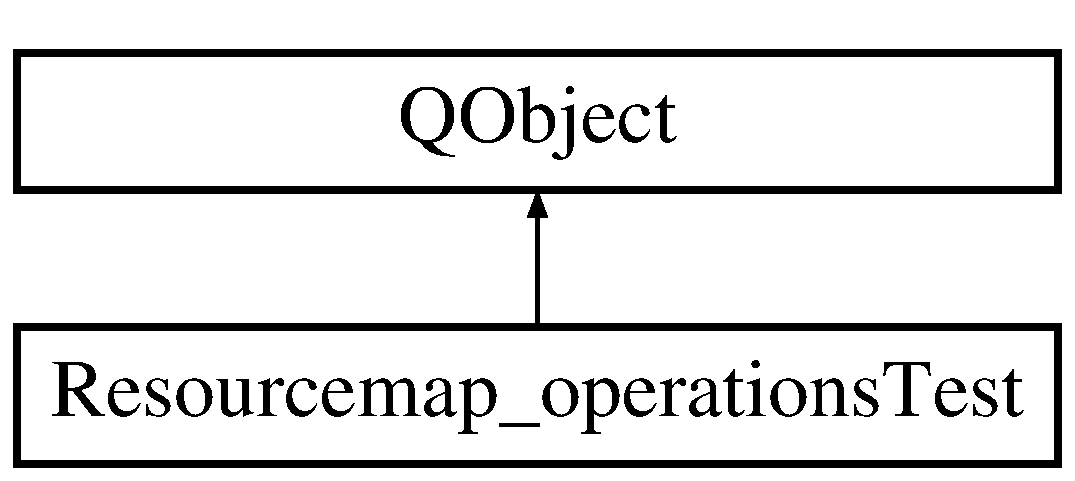
\includegraphics[height=2.000000cm]{classResourcemap__operationsTest}
\end{center}
\end{figure}
\subsection*{Public Member Functions}
\begin{DoxyCompactItemize}
\item 
\hyperlink{classResourcemap__operationsTest_a89e7689e4438827faab3d9b6845b9d84}{Resourcemap\-\_\-operations\-Test} ()
\end{DoxyCompactItemize}
\subsection*{Private Slots}
\begin{DoxyCompactItemize}
\item 
void \hyperlink{classResourcemap__operationsTest_a1f9ef8deb19bcdb07e4278ea142f7d2e}{merge\-\_\-\-R\-M} ()
\item 
void \hyperlink{classResourcemap__operationsTest_a993905385f445d0fcaba1d0fdea05c7e}{merge\-\_\-\-R\-M\-D} ()
\item 
void \hyperlink{classResourcemap__operationsTest_aefb8098c48eba65155ffbfff1c527c3b}{multiply} ()
\end{DoxyCompactItemize}
\subsection*{Private Attributes}
\begin{DoxyCompactItemize}
\item 
const \hyperlink{namespaceCourse_ab9a46ed9cd00485e318e5731ea2f78d9}{Resource\-Map} \hyperlink{classResourcemap__operationsTest_af1d531cadb8220f6477ab17b3a47f290}{R\-M1}
\item 
const \hyperlink{namespaceCourse_ab9a46ed9cd00485e318e5731ea2f78d9}{Resource\-Map} \hyperlink{classResourcemap__operationsTest_acfdf7232f48fe12d25658b10ec14fc0b}{R\-M\-\_\-\-S\-H\-O\-R\-T}
\item 
const \hyperlink{namespaceCourse_ab9a46ed9cd00485e318e5731ea2f78d9}{Resource\-Map} \hyperlink{classResourcemap__operationsTest_a20ba98848d1f7408a545cd740c58e57b}{R\-M\-\_\-\-N\-E\-G}
\item 
const \hyperlink{namespaceCourse_a0b96bae1a664dde34efbb1b42dea615e}{Resource\-Map\-Double} \hyperlink{classResourcemap__operationsTest_ad2af6115310ec9581944052356d9d44a}{R\-M\-D1}
\item 
const \hyperlink{namespaceCourse_a0b96bae1a664dde34efbb1b42dea615e}{Resource\-Map\-Double} \hyperlink{classResourcemap__operationsTest_a5dca1aa151e89d700b83a22f192c27ba}{R\-M\-D\-\_\-\-H\-A\-L\-F}
\end{DoxyCompactItemize}


\subsection{Constructor \& Destructor Documentation}
\hypertarget{classResourcemap__operationsTest_a89e7689e4438827faab3d9b6845b9d84}{\index{Resourcemap\-\_\-operations\-Test@{Resourcemap\-\_\-operations\-Test}!Resourcemap\-\_\-operations\-Test@{Resourcemap\-\_\-operations\-Test}}
\index{Resourcemap\-\_\-operations\-Test@{Resourcemap\-\_\-operations\-Test}!Resourcemap_operationsTest@{Resourcemap\-\_\-operations\-Test}}
\subsubsection[{Resourcemap\-\_\-operations\-Test}]{\setlength{\rightskip}{0pt plus 5cm}Resourcemap\-\_\-operations\-Test\-::\-Resourcemap\-\_\-operations\-Test (
\begin{DoxyParamCaption}
{}
\end{DoxyParamCaption}
)}}\label{classResourcemap__operationsTest_a89e7689e4438827faab3d9b6845b9d84}


\subsection{Member Function Documentation}
\hypertarget{classResourcemap__operationsTest_a1f9ef8deb19bcdb07e4278ea142f7d2e}{\index{Resourcemap\-\_\-operations\-Test@{Resourcemap\-\_\-operations\-Test}!merge\-\_\-\-R\-M@{merge\-\_\-\-R\-M}}
\index{merge\-\_\-\-R\-M@{merge\-\_\-\-R\-M}!Resourcemap_operationsTest@{Resourcemap\-\_\-operations\-Test}}
\subsubsection[{merge\-\_\-\-R\-M}]{\setlength{\rightskip}{0pt plus 5cm}void Resourcemap\-\_\-operations\-Test\-::merge\-\_\-\-R\-M (
\begin{DoxyParamCaption}
{}
\end{DoxyParamCaption}
)\hspace{0.3cm}{\ttfamily [private]}, {\ttfamily [slot]}}}\label{classResourcemap__operationsTest_a1f9ef8deb19bcdb07e4278ea142f7d2e}
\hypertarget{classResourcemap__operationsTest_a993905385f445d0fcaba1d0fdea05c7e}{\index{Resourcemap\-\_\-operations\-Test@{Resourcemap\-\_\-operations\-Test}!merge\-\_\-\-R\-M\-D@{merge\-\_\-\-R\-M\-D}}
\index{merge\-\_\-\-R\-M\-D@{merge\-\_\-\-R\-M\-D}!Resourcemap_operationsTest@{Resourcemap\-\_\-operations\-Test}}
\subsubsection[{merge\-\_\-\-R\-M\-D}]{\setlength{\rightskip}{0pt plus 5cm}void Resourcemap\-\_\-operations\-Test\-::merge\-\_\-\-R\-M\-D (
\begin{DoxyParamCaption}
{}
\end{DoxyParamCaption}
)\hspace{0.3cm}{\ttfamily [private]}, {\ttfamily [slot]}}}\label{classResourcemap__operationsTest_a993905385f445d0fcaba1d0fdea05c7e}
\hypertarget{classResourcemap__operationsTest_aefb8098c48eba65155ffbfff1c527c3b}{\index{Resourcemap\-\_\-operations\-Test@{Resourcemap\-\_\-operations\-Test}!multiply@{multiply}}
\index{multiply@{multiply}!Resourcemap_operationsTest@{Resourcemap\-\_\-operations\-Test}}
\subsubsection[{multiply}]{\setlength{\rightskip}{0pt plus 5cm}void Resourcemap\-\_\-operations\-Test\-::multiply (
\begin{DoxyParamCaption}
{}
\end{DoxyParamCaption}
)\hspace{0.3cm}{\ttfamily [private]}, {\ttfamily [slot]}}}\label{classResourcemap__operationsTest_aefb8098c48eba65155ffbfff1c527c3b}


\subsection{Member Data Documentation}
\hypertarget{classResourcemap__operationsTest_af1d531cadb8220f6477ab17b3a47f290}{\index{Resourcemap\-\_\-operations\-Test@{Resourcemap\-\_\-operations\-Test}!R\-M1@{R\-M1}}
\index{R\-M1@{R\-M1}!Resourcemap_operationsTest@{Resourcemap\-\_\-operations\-Test}}
\subsubsection[{R\-M1}]{\setlength{\rightskip}{0pt plus 5cm}const {\bf Resource\-Map} Resourcemap\-\_\-operations\-Test\-::\-R\-M1\hspace{0.3cm}{\ttfamily [private]}}}\label{classResourcemap__operationsTest_af1d531cadb8220f6477ab17b3a47f290}
{\bfseries Initial value\-:}
\begin{DoxyCode}
= \{
        \{\hyperlink{namespaceCourse_a02d49c04029594d4adba79b84bb85f65ae3def61eb1a9033cc0b0d1d2c3c6ff84}{NONE}, 10\},
        \{\hyperlink{namespaceCourse_a02d49c04029594d4adba79b84bb85f65aff016add6bbbdbb44abf1d2d7f215ec0}{MONEY}, 20\},
        \{\hyperlink{namespaceCourse_a02d49c04029594d4adba79b84bb85f65a7018c47af38bfc1390a89e70b4cf4760}{FOOD}, 30\},
        \{\hyperlink{namespaceCourse_a02d49c04029594d4adba79b84bb85f65a87287be3009253b983ffb2e9f91eef22}{WOOD}, 40\},
        \{\hyperlink{namespaceCourse_a02d49c04029594d4adba79b84bb85f65a8598c3079c2be7785410e724cc190229}{STONE}, 50\},
        \{\hyperlink{namespaceCourse_a02d49c04029594d4adba79b84bb85f65af416a215c7dad21349df38d35be0a1e1}{ORE}, 60\}
    \}
\end{DoxyCode}
\hypertarget{classResourcemap__operationsTest_a20ba98848d1f7408a545cd740c58e57b}{\index{Resourcemap\-\_\-operations\-Test@{Resourcemap\-\_\-operations\-Test}!R\-M\-\_\-\-N\-E\-G@{R\-M\-\_\-\-N\-E\-G}}
\index{R\-M\-\_\-\-N\-E\-G@{R\-M\-\_\-\-N\-E\-G}!Resourcemap_operationsTest@{Resourcemap\-\_\-operations\-Test}}
\subsubsection[{R\-M\-\_\-\-N\-E\-G}]{\setlength{\rightskip}{0pt plus 5cm}const {\bf Resource\-Map} Resourcemap\-\_\-operations\-Test\-::\-R\-M\-\_\-\-N\-E\-G\hspace{0.3cm}{\ttfamily [private]}}}\label{classResourcemap__operationsTest_a20ba98848d1f7408a545cd740c58e57b}
{\bfseries Initial value\-:}
\begin{DoxyCode}
= \{
        \{\hyperlink{namespaceCourse_a02d49c04029594d4adba79b84bb85f65ae3def61eb1a9033cc0b0d1d2c3c6ff84}{NONE}, -5\},
        \{\hyperlink{namespaceCourse_a02d49c04029594d4adba79b84bb85f65aff016add6bbbdbb44abf1d2d7f215ec0}{MONEY}, 6\},
        \{\hyperlink{namespaceCourse_a02d49c04029594d4adba79b84bb85f65a7018c47af38bfc1390a89e70b4cf4760}{FOOD}, -1\},
        \{\hyperlink{namespaceCourse_a02d49c04029594d4adba79b84bb85f65a87287be3009253b983ffb2e9f91eef22}{WOOD}, -20\},
        \{\hyperlink{namespaceCourse_a02d49c04029594d4adba79b84bb85f65a8598c3079c2be7785410e724cc190229}{STONE}, 0\},
        \{\hyperlink{namespaceCourse_a02d49c04029594d4adba79b84bb85f65af416a215c7dad21349df38d35be0a1e1}{ORE}, -100\}
    \}
\end{DoxyCode}
\hypertarget{classResourcemap__operationsTest_acfdf7232f48fe12d25658b10ec14fc0b}{\index{Resourcemap\-\_\-operations\-Test@{Resourcemap\-\_\-operations\-Test}!R\-M\-\_\-\-S\-H\-O\-R\-T@{R\-M\-\_\-\-S\-H\-O\-R\-T}}
\index{R\-M\-\_\-\-S\-H\-O\-R\-T@{R\-M\-\_\-\-S\-H\-O\-R\-T}!Resourcemap_operationsTest@{Resourcemap\-\_\-operations\-Test}}
\subsubsection[{R\-M\-\_\-\-S\-H\-O\-R\-T}]{\setlength{\rightskip}{0pt plus 5cm}const {\bf Resource\-Map} Resourcemap\-\_\-operations\-Test\-::\-R\-M\-\_\-\-S\-H\-O\-R\-T\hspace{0.3cm}{\ttfamily [private]}}}\label{classResourcemap__operationsTest_acfdf7232f48fe12d25658b10ec14fc0b}
{\bfseries Initial value\-:}
\begin{DoxyCode}
= \{
        \{\hyperlink{namespaceCourse_a02d49c04029594d4adba79b84bb85f65ae3def61eb1a9033cc0b0d1d2c3c6ff84}{NONE}, 5\},
        \{\hyperlink{namespaceCourse_a02d49c04029594d4adba79b84bb85f65aff016add6bbbdbb44abf1d2d7f215ec0}{MONEY}, 5\},
        \{\hyperlink{namespaceCourse_a02d49c04029594d4adba79b84bb85f65a7018c47af38bfc1390a89e70b4cf4760}{FOOD}, 5\}
    \}
\end{DoxyCode}
\hypertarget{classResourcemap__operationsTest_ad2af6115310ec9581944052356d9d44a}{\index{Resourcemap\-\_\-operations\-Test@{Resourcemap\-\_\-operations\-Test}!R\-M\-D1@{R\-M\-D1}}
\index{R\-M\-D1@{R\-M\-D1}!Resourcemap_operationsTest@{Resourcemap\-\_\-operations\-Test}}
\subsubsection[{R\-M\-D1}]{\setlength{\rightskip}{0pt plus 5cm}const {\bf Resource\-Map\-Double} Resourcemap\-\_\-operations\-Test\-::\-R\-M\-D1\hspace{0.3cm}{\ttfamily [private]}}}\label{classResourcemap__operationsTest_ad2af6115310ec9581944052356d9d44a}
{\bfseries Initial value\-:}
\begin{DoxyCode}
= \{
        \{\hyperlink{namespaceCourse_a02d49c04029594d4adba79b84bb85f65ae3def61eb1a9033cc0b0d1d2c3c6ff84}{NONE}, 1.0\},
        \{\hyperlink{namespaceCourse_a02d49c04029594d4adba79b84bb85f65aff016add6bbbdbb44abf1d2d7f215ec0}{MONEY}, 2.0\},
        \{\hyperlink{namespaceCourse_a02d49c04029594d4adba79b84bb85f65a7018c47af38bfc1390a89e70b4cf4760}{FOOD}, 3.0\},
        \{\hyperlink{namespaceCourse_a02d49c04029594d4adba79b84bb85f65a87287be3009253b983ffb2e9f91eef22}{WOOD}, 4.0\},
        \{\hyperlink{namespaceCourse_a02d49c04029594d4adba79b84bb85f65a8598c3079c2be7785410e724cc190229}{STONE}, 5.0\},
        \{\hyperlink{namespaceCourse_a02d49c04029594d4adba79b84bb85f65af416a215c7dad21349df38d35be0a1e1}{ORE}, 6.0\}
    \}
\end{DoxyCode}
\hypertarget{classResourcemap__operationsTest_a5dca1aa151e89d700b83a22f192c27ba}{\index{Resourcemap\-\_\-operations\-Test@{Resourcemap\-\_\-operations\-Test}!R\-M\-D\-\_\-\-H\-A\-L\-F@{R\-M\-D\-\_\-\-H\-A\-L\-F}}
\index{R\-M\-D\-\_\-\-H\-A\-L\-F@{R\-M\-D\-\_\-\-H\-A\-L\-F}!Resourcemap_operationsTest@{Resourcemap\-\_\-operations\-Test}}
\subsubsection[{R\-M\-D\-\_\-\-H\-A\-L\-F}]{\setlength{\rightskip}{0pt plus 5cm}const {\bf Resource\-Map\-Double} Resourcemap\-\_\-operations\-Test\-::\-R\-M\-D\-\_\-\-H\-A\-L\-F\hspace{0.3cm}{\ttfamily [private]}}}\label{classResourcemap__operationsTest_a5dca1aa151e89d700b83a22f192c27ba}
{\bfseries Initial value\-:}
\begin{DoxyCode}
= \{
        \{\hyperlink{namespaceCourse_a02d49c04029594d4adba79b84bb85f65ae3def61eb1a9033cc0b0d1d2c3c6ff84}{NONE}, 0.5\},
        \{\hyperlink{namespaceCourse_a02d49c04029594d4adba79b84bb85f65aff016add6bbbdbb44abf1d2d7f215ec0}{MONEY}, 0.5\},
        \{\hyperlink{namespaceCourse_a02d49c04029594d4adba79b84bb85f65a7018c47af38bfc1390a89e70b4cf4760}{FOOD}, 0.5\},
        \{\hyperlink{namespaceCourse_a02d49c04029594d4adba79b84bb85f65a87287be3009253b983ffb2e9f91eef22}{WOOD}, 0.5\},
        \{\hyperlink{namespaceCourse_a02d49c04029594d4adba79b84bb85f65a8598c3079c2be7785410e724cc190229}{STONE}, 0.5\},
        \{\hyperlink{namespaceCourse_a02d49c04029594d4adba79b84bb85f65af416a215c7dad21349df38d35be0a1e1}{ORE}, 0.5\}
    \}
\end{DoxyCode}


The documentation for this class was generated from the following file\-:\begin{DoxyCompactItemize}
\item 
Course/\-Unit\-Tests/resourcemap\-\_\-operations/\hyperlink{tst__resourcemap__operationstest_8cpp}{tst\-\_\-resourcemap\-\_\-operationstest.\-cpp}\end{DoxyCompactItemize}

\hypertarget{classGame_1_1SawMill}{\section{Game\-:\-:Saw\-Mill Class Reference}
\label{classGame_1_1SawMill}\index{Game\-::\-Saw\-Mill@{Game\-::\-Saw\-Mill}}
}


The Sawmill class represents a sawmill-\/building in the game.  




{\ttfamily \#include $<$sawmill.\-hh$>$}

Inheritance diagram for Game\-:\-:Saw\-Mill\-:\begin{figure}[H]
\begin{center}
\leavevmode
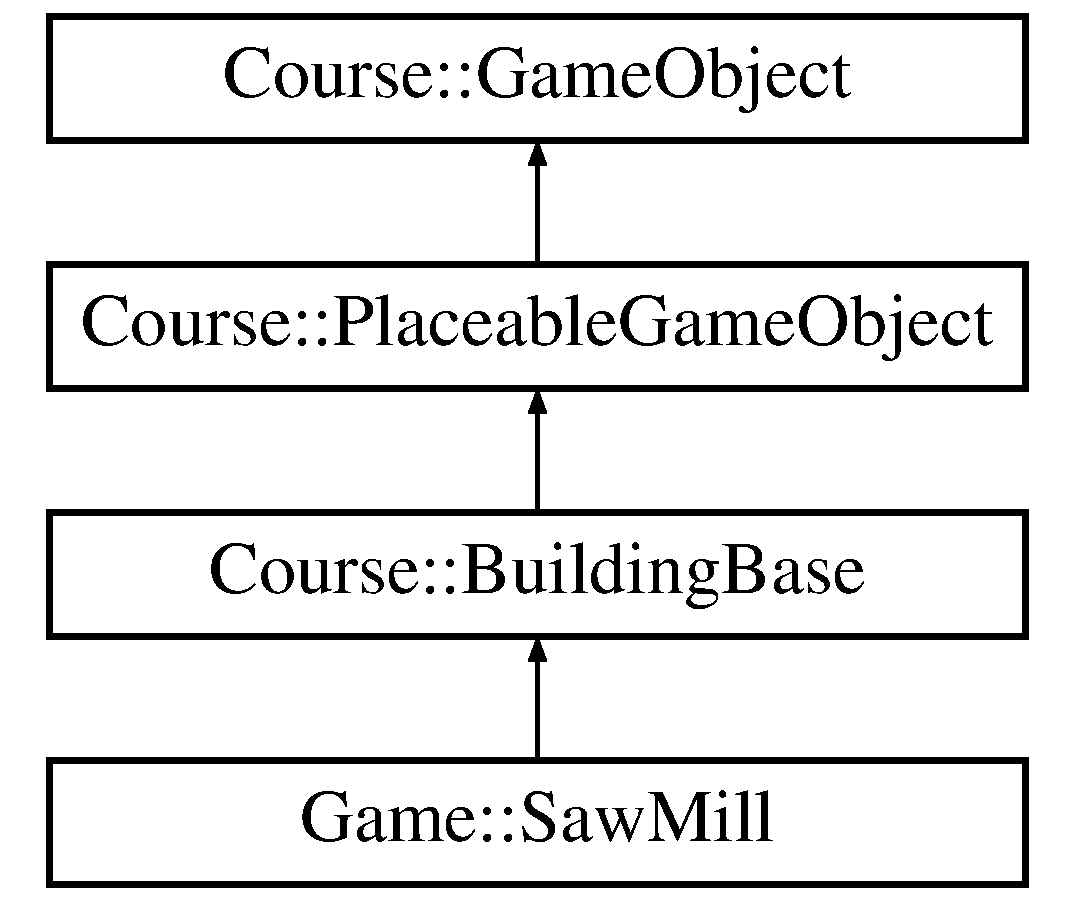
\includegraphics[height=4.000000cm]{classGame_1_1SawMill}
\end{center}
\end{figure}
\subsection*{Public Member Functions}
\begin{DoxyCompactItemize}
\item 
\hyperlink{classGame_1_1SawMill_a95000ee2a18a7c1bf3a34c84b1c2cf8d}{Saw\-Mill} ()=delete
\begin{DoxyCompactList}\small\item\em Disabled parameterless constructor. \end{DoxyCompactList}\item 
\hyperlink{classGame_1_1SawMill_a981300064bd66ef5e752a1d00e516bfc}{Saw\-Mill} (const std\-::shared\-\_\-ptr$<$ \hyperlink{classGame_1_1GameEventHandler}{Game\-Event\-Handler} $>$ \&eventhandler, const std\-::shared\-\_\-ptr$<$ \hyperlink{classGame_1_1ObjectManager}{Object\-Manager} $>$ \&objectmanager, const std\-::shared\-\_\-ptr$<$ \hyperlink{classGame_1_1Player}{Player} $>$ \&owner, const int \&tilespaces=1, const \hyperlink{namespaceCourse_ab9a46ed9cd00485e318e5731ea2f78d9}{Course\-::\-Resource\-Map} \&buildcost=\hyperlink{namespaceGame_1_1ConstResourceMaps_a8101879b3f9a231535e629475969da07}{Game\-::\-Const\-Resource\-Maps\-::\-S\-A\-W\-M\-I\-L\-L\-\_\-\-B\-U\-I\-L\-D\-\_\-\-C\-O\-S\-T}, const \hyperlink{namespaceCourse_ab9a46ed9cd00485e318e5731ea2f78d9}{Course\-::\-Resource\-Map} \&production=\hyperlink{namespaceGame_1_1ConstResourceMaps_a1302532b63eb3d623779fb539dd767e8}{Game\-::\-Const\-Resource\-Maps\-::\-S\-A\-W\-M\-I\-L\-L\-\_\-\-P\-R\-O\-D\-U\-C\-T\-I\-O\-N})
\begin{DoxyCompactList}\small\item\em Constructor for the class. \end{DoxyCompactList}\item 
virtual \hyperlink{classGame_1_1SawMill_a9755f338538ca6bfec391f538ee435d8}{$\sim$\-Saw\-Mill} ()=default
\begin{DoxyCompactList}\small\item\em Default destructor. \end{DoxyCompactList}\item 
virtual std\-::string \hyperlink{classGame_1_1SawMill_a1dd6fd6bce2044107b121f3bbf012691}{get\-Type} () const override
\end{DoxyCompactItemize}
\subsection*{Additional Inherited Members}


\subsection{Detailed Description}
The Sawmill class represents a sawmill-\/building in the game. 

The sawmill adds 1 base-\/production for money, 2 for food and 5 for wood. 

\subsection{Constructor \& Destructor Documentation}
\hypertarget{classGame_1_1SawMill_a95000ee2a18a7c1bf3a34c84b1c2cf8d}{\index{Game\-::\-Saw\-Mill@{Game\-::\-Saw\-Mill}!Saw\-Mill@{Saw\-Mill}}
\index{Saw\-Mill@{Saw\-Mill}!Game::SawMill@{Game\-::\-Saw\-Mill}}
\subsubsection[{Saw\-Mill}]{\setlength{\rightskip}{0pt plus 5cm}Game\-::\-Saw\-Mill\-::\-Saw\-Mill (
\begin{DoxyParamCaption}
{}
\end{DoxyParamCaption}
)\hspace{0.3cm}{\ttfamily [delete]}}}\label{classGame_1_1SawMill_a95000ee2a18a7c1bf3a34c84b1c2cf8d}


Disabled parameterless constructor. 

\hypertarget{classGame_1_1SawMill_a981300064bd66ef5e752a1d00e516bfc}{\index{Game\-::\-Saw\-Mill@{Game\-::\-Saw\-Mill}!Saw\-Mill@{Saw\-Mill}}
\index{Saw\-Mill@{Saw\-Mill}!Game::SawMill@{Game\-::\-Saw\-Mill}}
\subsubsection[{Saw\-Mill}]{\setlength{\rightskip}{0pt plus 5cm}Game\-::\-Saw\-Mill\-::\-Saw\-Mill (
\begin{DoxyParamCaption}
\item[{const std\-::shared\-\_\-ptr$<$ {\bf Game\-Event\-Handler} $>$ \&}]{eventhandler, }
\item[{const std\-::shared\-\_\-ptr$<$ {\bf Object\-Manager} $>$ \&}]{objectmanager, }
\item[{const std\-::shared\-\_\-ptr$<$ {\bf Player} $>$ \&}]{owner, }
\item[{const int \&}]{tilespaces = {\ttfamily 1}, }
\item[{const {\bf Course\-::\-Resource\-Map} \&}]{buildcost = {\ttfamily {\bf Game\-::\-Const\-Resource\-Maps\-::\-S\-A\-W\-M\-I\-L\-L\-\_\-\-B\-U\-I\-L\-D\-\_\-\-C\-O\-S\-T}}, }
\item[{const {\bf Course\-::\-Resource\-Map} \&}]{production = {\ttfamily {\bf Game\-::\-Const\-Resource\-Maps\-::\-S\-A\-W\-M\-I\-L\-L\-\_\-\-P\-R\-O\-D\-U\-C\-T\-I\-O\-N}}}
\end{DoxyParamCaption}
)\hspace{0.3cm}{\ttfamily [explicit]}}}\label{classGame_1_1SawMill_a981300064bd66ef5e752a1d00e516bfc}


Constructor for the class. 


\begin{DoxyParams}{Parameters}
{\em eventhandler} & points to the student's \hyperlink{classGame_1_1GameEventHandler}{Game\-Event\-Handler}. \\
\hline
{\em owner} & points to the owning player. \\
\hline
{\em tile} & points to the tile upon which the building is constructed.\\
\hline
\end{DoxyParams}
\begin{DoxyPostcond}{Postcondition}
Exception Guarantee\-: No guarantee. 
\end{DoxyPostcond}

\begin{DoxyExceptions}{Exceptions}
{\em Owner\-Conflict} & -\/ if the building conflicts with tile's ownership. \\
\hline
\end{DoxyExceptions}
\hypertarget{classGame_1_1SawMill_a9755f338538ca6bfec391f538ee435d8}{\index{Game\-::\-Saw\-Mill@{Game\-::\-Saw\-Mill}!$\sim$\-Saw\-Mill@{$\sim$\-Saw\-Mill}}
\index{$\sim$\-Saw\-Mill@{$\sim$\-Saw\-Mill}!Game::SawMill@{Game\-::\-Saw\-Mill}}
\subsubsection[{$\sim$\-Saw\-Mill}]{\setlength{\rightskip}{0pt plus 5cm}virtual Game\-::\-Saw\-Mill\-::$\sim$\-Saw\-Mill (
\begin{DoxyParamCaption}
{}
\end{DoxyParamCaption}
)\hspace{0.3cm}{\ttfamily [virtual]}, {\ttfamily [default]}}}\label{classGame_1_1SawMill_a9755f338538ca6bfec391f538ee435d8}


Default destructor. 



\subsection{Member Function Documentation}
\hypertarget{classGame_1_1SawMill_a1dd6fd6bce2044107b121f3bbf012691}{\index{Game\-::\-Saw\-Mill@{Game\-::\-Saw\-Mill}!get\-Type@{get\-Type}}
\index{get\-Type@{get\-Type}!Game::SawMill@{Game\-::\-Saw\-Mill}}
\subsubsection[{get\-Type}]{\setlength{\rightskip}{0pt plus 5cm}std\-::string Game\-::\-Saw\-Mill\-::get\-Type (
\begin{DoxyParamCaption}
{}
\end{DoxyParamCaption}
) const\hspace{0.3cm}{\ttfamily [override]}, {\ttfamily [virtual]}}}\label{classGame_1_1SawMill_a1dd6fd6bce2044107b121f3bbf012691}






Reimplemented from \hyperlink{classCourse_1_1BuildingBase_ac2cc44e08dc73d05b1617bf71295baaf}{Course\-::\-Building\-Base}.



The documentation for this class was generated from the following files\-:\begin{DoxyCompactItemize}
\item 
Game/buildings/\hyperlink{sawmill_8hh}{sawmill.\-hh}\item 
Game/buildings/\hyperlink{sawmill_8cpp}{sawmill.\-cpp}\end{DoxyCompactItemize}

\hypertarget{classGame_1_1SawMillWorker}{\section{Game\-:\-:Saw\-Mill\-Worker Class Reference}
\label{classGame_1_1SawMillWorker}\index{Game\-::\-Saw\-Mill\-Worker@{Game\-::\-Saw\-Mill\-Worker}}
}


The \hyperlink{classGame_1_1SawMillWorker}{Saw\-Mill\-Worker} class represents a saw mill worker in the game.  




{\ttfamily \#include $<$sawmillworker.\-h$>$}

Inheritance diagram for Game\-:\-:Saw\-Mill\-Worker\-:\begin{figure}[H]
\begin{center}
\leavevmode
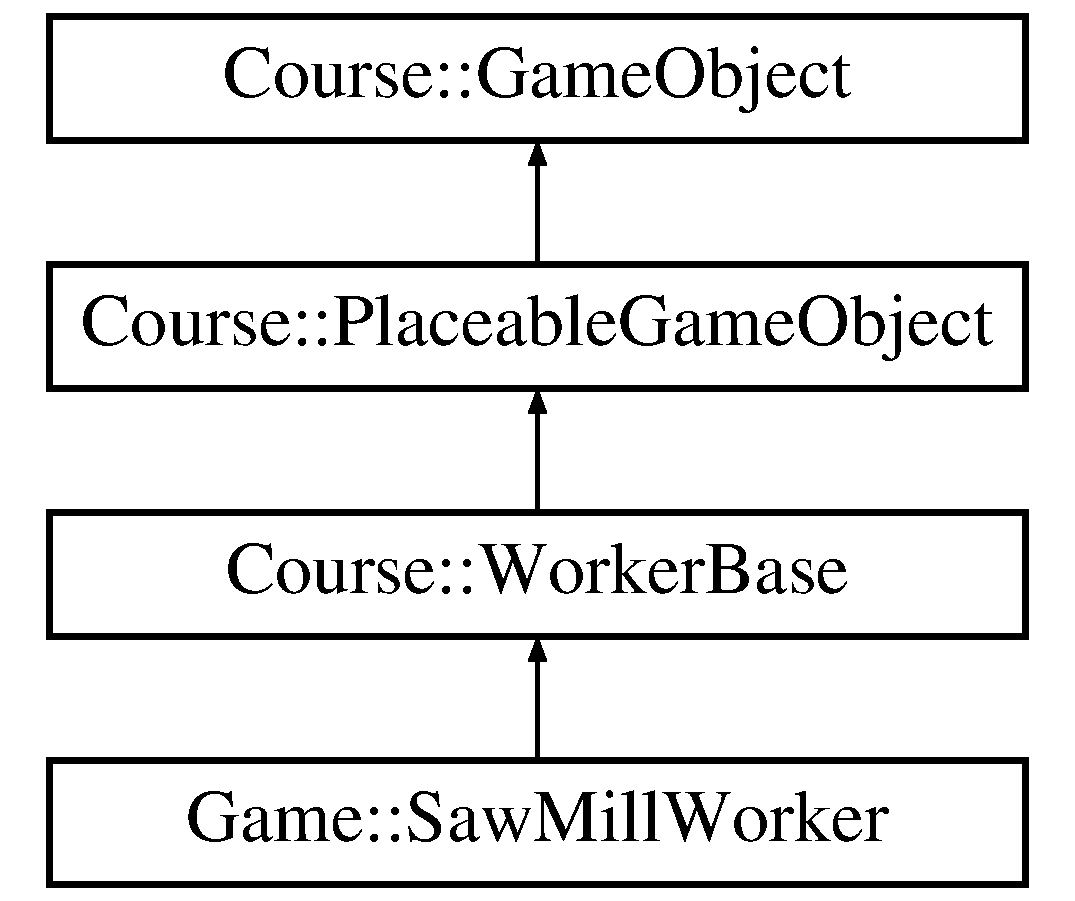
\includegraphics[height=4.000000cm]{classGame_1_1SawMillWorker}
\end{center}
\end{figure}
\subsection*{Public Member Functions}
\begin{DoxyCompactItemize}
\item 
\hyperlink{classGame_1_1SawMillWorker_ae2d01dff4f059f5ab575d1b416764f52}{Saw\-Mill\-Worker} ()=delete
\begin{DoxyCompactList}\small\item\em Disabled parameterless constructor. \end{DoxyCompactList}\item 
\hyperlink{classGame_1_1SawMillWorker_adc9fe554404554f5051a7ed7b057bbc3}{Saw\-Mill\-Worker} (const std\-::shared\-\_\-ptr$<$ \hyperlink{classCourse_1_1iGameEventHandler}{Course\-::i\-Game\-Event\-Handler} $>$ \&eventhandler, const std\-::shared\-\_\-ptr$<$ \hyperlink{classCourse_1_1iObjectManager}{Course\-::i\-Object\-Manager} $>$ \&objectmanager, const std\-::shared\-\_\-ptr$<$ \hyperlink{classCourse_1_1PlayerBase}{Course\-::\-Player\-Base} $>$ \&owner, const int \&tilespaces=1, const \hyperlink{namespaceCourse_ab9a46ed9cd00485e318e5731ea2f78d9}{Course\-::\-Resource\-Map} \&cost=\hyperlink{namespaceGame_1_1ConstResourceMaps_aece4521104576e9af5ab8635b786c840}{Game\-::\-Const\-Resource\-Maps\-::\-S\-M\-W\-\_\-\-R\-E\-C\-R\-U\-I\-T\-M\-E\-N\-T\-\_\-\-C\-O\-S\-T}, const \hyperlink{namespaceCourse_a0b96bae1a664dde34efbb1b42dea615e}{Course\-::\-Resource\-Map\-Double} \&efficiency=\hyperlink{namespaceGame_1_1ConstResourceMaps_aa229959dcf7750d06878db7f5c4d0bae}{Game\-::\-Const\-Resource\-Maps\-::\-S\-M\-W\-\_\-\-W\-O\-R\-K\-E\-R\-\_\-\-E\-F\-F\-I\-C\-I\-E\-N\-C\-Y})
\begin{DoxyCompactList}\small\item\em Constructor for the class. \end{DoxyCompactList}\item 
virtual \hyperlink{classGame_1_1SawMillWorker_a3eff92aacde38a3ee5b27df21b75289b}{$\sim$\-Saw\-Mill\-Worker} ()=default
\begin{DoxyCompactList}\small\item\em Default destructor. \end{DoxyCompactList}\item 
virtual std\-::string \hyperlink{classGame_1_1SawMillWorker_af64ec6de521d31ec3fdc885a3bc69cba}{get\-Type} () const override
\item 
virtual bool \hyperlink{classGame_1_1SawMillWorker_a435e13b35d129a453d7fdfcd60b6dc42}{can\-Be\-Placed\-On\-Tile} (const std\-::shared\-\_\-ptr$<$ \hyperlink{classCourse_1_1TileBase}{Course\-::\-Tile\-Base} $>$ \&target) const override
\begin{DoxyCompactList}\small\item\em Check if the worker can be placed on the Tile according to it's placement rule. Only rule is that the Tile must have same owner as the worker. \end{DoxyCompactList}\item 
virtual void \hyperlink{classGame_1_1SawMillWorker_af344bff415417cb0c2744b038872221a}{do\-Special\-Action} () override
\begin{DoxyCompactList}\small\item\em Performs the Worker's default action. Does nothing as this is not implemented. \end{DoxyCompactList}\item 
virtual const \\*
\hyperlink{namespaceCourse_a0b96bae1a664dde34efbb1b42dea615e}{Course\-::\-Resource\-Map\-Double} \hyperlink{classGame_1_1SawMillWorker_a51596a8864954a22c6b69303b5e408d8}{tile\-Work\-Action} () override
\begin{DoxyCompactList}\small\item\em Returns Worker's efficiency at resource production. Worker consumes F\-O\-O\-D and M\-O\-N\-E\-Y. Resource consumption and resource focus determine final multiplier that is based on W\-O\-R\-K\-E\-R\-\_\-\-E\-F\-F\-I\-C\-I\-E\-N\-C\-Y. \end{DoxyCompactList}\end{DoxyCompactItemize}
\subsection*{Additional Inherited Members}


\subsection{Detailed Description}
The \hyperlink{classGame_1_1SawMillWorker}{Saw\-Mill\-Worker} class represents a saw mill worker in the game. 

Worker has following production-\/efficiency\-: \par

\begin{DoxyItemize}
\item Money -\/ 0.\-25 \par

\item Food -\/ 0.\-25 \par

\item Wood -\/ 2.\-00 \par

\item Stone -\/ 0.\-25 \par

\item Ore -\/ 0.\-25 \par
 \hyperlink{classGame_1_1SawMillWorker}{Saw\-Mill\-Worker} consume Food and money. \par

\item 2 Food -\/ Or \hyperlink{classGame_1_1SawMillWorker}{Saw\-Mill\-Worker} refuses to work. \par

\item 2 Money -\/ Or \hyperlink{classGame_1_1SawMillWorker}{Saw\-Mill\-Worker} works at 50\% efficiency. 
\end{DoxyItemize}

\subsection{Constructor \& Destructor Documentation}
\hypertarget{classGame_1_1SawMillWorker_ae2d01dff4f059f5ab575d1b416764f52}{\index{Game\-::\-Saw\-Mill\-Worker@{Game\-::\-Saw\-Mill\-Worker}!Saw\-Mill\-Worker@{Saw\-Mill\-Worker}}
\index{Saw\-Mill\-Worker@{Saw\-Mill\-Worker}!Game::SawMillWorker@{Game\-::\-Saw\-Mill\-Worker}}
\subsubsection[{Saw\-Mill\-Worker}]{\setlength{\rightskip}{0pt plus 5cm}Game\-::\-Saw\-Mill\-Worker\-::\-Saw\-Mill\-Worker (
\begin{DoxyParamCaption}
{}
\end{DoxyParamCaption}
)\hspace{0.3cm}{\ttfamily [delete]}}}\label{classGame_1_1SawMillWorker_ae2d01dff4f059f5ab575d1b416764f52}


Disabled parameterless constructor. 

\hypertarget{classGame_1_1SawMillWorker_adc9fe554404554f5051a7ed7b057bbc3}{\index{Game\-::\-Saw\-Mill\-Worker@{Game\-::\-Saw\-Mill\-Worker}!Saw\-Mill\-Worker@{Saw\-Mill\-Worker}}
\index{Saw\-Mill\-Worker@{Saw\-Mill\-Worker}!Game::SawMillWorker@{Game\-::\-Saw\-Mill\-Worker}}
\subsubsection[{Saw\-Mill\-Worker}]{\setlength{\rightskip}{0pt plus 5cm}Game\-::\-Saw\-Mill\-Worker\-::\-Saw\-Mill\-Worker (
\begin{DoxyParamCaption}
\item[{const std\-::shared\-\_\-ptr$<$ {\bf Course\-::i\-Game\-Event\-Handler} $>$ \&}]{eventhandler, }
\item[{const std\-::shared\-\_\-ptr$<$ {\bf Course\-::i\-Object\-Manager} $>$ \&}]{objectmanager, }
\item[{const std\-::shared\-\_\-ptr$<$ {\bf Course\-::\-Player\-Base} $>$ \&}]{owner, }
\item[{const int \&}]{tilespaces = {\ttfamily 1}, }
\item[{const {\bf Course\-::\-Resource\-Map} \&}]{cost = {\ttfamily {\bf Game\-::\-Const\-Resource\-Maps\-::\-S\-M\-W\-\_\-\-R\-E\-C\-R\-U\-I\-T\-M\-E\-N\-T\-\_\-\-C\-O\-S\-T}}, }
\item[{const {\bf Course\-::\-Resource\-Map\-Double} \&}]{efficiency = {\ttfamily {\bf Game\-::\-Const\-Resource\-Maps\-::\-S\-M\-W\-\_\-\-W\-O\-R\-K\-E\-R\-\_\-\-E\-F\-F\-I\-C\-I\-E\-N\-C\-Y}}}
\end{DoxyParamCaption}
)}}\label{classGame_1_1SawMillWorker_adc9fe554404554f5051a7ed7b057bbc3}


Constructor for the class. 


\begin{DoxyParams}{Parameters}
{\em eventhandler} & points to the student's \hyperlink{classGame_1_1GameEventHandler}{Game\-Event\-Handler}. \\
\hline
{\em objectmanager} & points to the \hyperlink{classGame_1_1ObjectManager}{Object\-Manager}. \\
\hline
{\em owner} & points to the owning player. \\
\hline
{\em tilespaces} & defines how many spaces the worker takes on tile \\
\hline
{\em cost} & defines how much the worker costs \\
\hline
{\em efficiency} & defines how much and what the worker produces \\
\hline
\end{DoxyParams}
\hypertarget{classGame_1_1SawMillWorker_a3eff92aacde38a3ee5b27df21b75289b}{\index{Game\-::\-Saw\-Mill\-Worker@{Game\-::\-Saw\-Mill\-Worker}!$\sim$\-Saw\-Mill\-Worker@{$\sim$\-Saw\-Mill\-Worker}}
\index{$\sim$\-Saw\-Mill\-Worker@{$\sim$\-Saw\-Mill\-Worker}!Game::SawMillWorker@{Game\-::\-Saw\-Mill\-Worker}}
\subsubsection[{$\sim$\-Saw\-Mill\-Worker}]{\setlength{\rightskip}{0pt plus 5cm}virtual Game\-::\-Saw\-Mill\-Worker\-::$\sim$\-Saw\-Mill\-Worker (
\begin{DoxyParamCaption}
{}
\end{DoxyParamCaption}
)\hspace{0.3cm}{\ttfamily [virtual]}, {\ttfamily [default]}}}\label{classGame_1_1SawMillWorker_a3eff92aacde38a3ee5b27df21b75289b}


Default destructor. 



\subsection{Member Function Documentation}
\hypertarget{classGame_1_1SawMillWorker_a435e13b35d129a453d7fdfcd60b6dc42}{\index{Game\-::\-Saw\-Mill\-Worker@{Game\-::\-Saw\-Mill\-Worker}!can\-Be\-Placed\-On\-Tile@{can\-Be\-Placed\-On\-Tile}}
\index{can\-Be\-Placed\-On\-Tile@{can\-Be\-Placed\-On\-Tile}!Game::SawMillWorker@{Game\-::\-Saw\-Mill\-Worker}}
\subsubsection[{can\-Be\-Placed\-On\-Tile}]{\setlength{\rightskip}{0pt plus 5cm}bool Game\-::\-Saw\-Mill\-Worker\-::can\-Be\-Placed\-On\-Tile (
\begin{DoxyParamCaption}
\item[{const std\-::shared\-\_\-ptr$<$ {\bf Course\-::\-Tile\-Base} $>$ \&}]{target}
\end{DoxyParamCaption}
) const\hspace{0.3cm}{\ttfamily [override]}, {\ttfamily [virtual]}}}\label{classGame_1_1SawMillWorker_a435e13b35d129a453d7fdfcd60b6dc42}


Check if the worker can be placed on the Tile according to it's placement rule. Only rule is that the Tile must have same owner as the worker. 


\begin{DoxyParams}{Parameters}
{\em target} & is the Tile that worker is being placed on. \\
\hline
\end{DoxyParams}
\begin{DoxyReturn}{Returns}
True -\/ If baseclass' method return true and target Tile has space for worker. False -\/ If both conditions aren't met. 
\end{DoxyReturn}
\begin{DoxyNote}{Note}
Override to change placement rules for derived worker. 
\end{DoxyNote}
\begin{DoxyPostcond}{Postcondition}
Exception guarantee\-: Basic 
\end{DoxyPostcond}


Reimplemented from \hyperlink{classCourse_1_1WorkerBase_ad80874970ab91bca95b9d3f959e838d2}{Course\-::\-Worker\-Base}.

\hypertarget{classGame_1_1SawMillWorker_af344bff415417cb0c2744b038872221a}{\index{Game\-::\-Saw\-Mill\-Worker@{Game\-::\-Saw\-Mill\-Worker}!do\-Special\-Action@{do\-Special\-Action}}
\index{do\-Special\-Action@{do\-Special\-Action}!Game::SawMillWorker@{Game\-::\-Saw\-Mill\-Worker}}
\subsubsection[{do\-Special\-Action}]{\setlength{\rightskip}{0pt plus 5cm}void Game\-::\-Saw\-Mill\-Worker\-::do\-Special\-Action (
\begin{DoxyParamCaption}
{}
\end{DoxyParamCaption}
)\hspace{0.3cm}{\ttfamily [override]}, {\ttfamily [virtual]}}}\label{classGame_1_1SawMillWorker_af344bff415417cb0c2744b038872221a}


Performs the Worker's default action. Does nothing as this is not implemented. 



Implements \hyperlink{classCourse_1_1WorkerBase_a78553f35740e1c07d8f1071b5fc82212}{Course\-::\-Worker\-Base}.

\hypertarget{classGame_1_1SawMillWorker_af64ec6de521d31ec3fdc885a3bc69cba}{\index{Game\-::\-Saw\-Mill\-Worker@{Game\-::\-Saw\-Mill\-Worker}!get\-Type@{get\-Type}}
\index{get\-Type@{get\-Type}!Game::SawMillWorker@{Game\-::\-Saw\-Mill\-Worker}}
\subsubsection[{get\-Type}]{\setlength{\rightskip}{0pt plus 5cm}std\-::string Game\-::\-Saw\-Mill\-Worker\-::get\-Type (
\begin{DoxyParamCaption}
{}
\end{DoxyParamCaption}
) const\hspace{0.3cm}{\ttfamily [override]}, {\ttfamily [virtual]}}}\label{classGame_1_1SawMillWorker_af64ec6de521d31ec3fdc885a3bc69cba}






Reimplemented from \hyperlink{classCourse_1_1WorkerBase_afe6049810eec47fffe2c2a7334564ef9}{Course\-::\-Worker\-Base}.

\hypertarget{classGame_1_1SawMillWorker_a51596a8864954a22c6b69303b5e408d8}{\index{Game\-::\-Saw\-Mill\-Worker@{Game\-::\-Saw\-Mill\-Worker}!tile\-Work\-Action@{tile\-Work\-Action}}
\index{tile\-Work\-Action@{tile\-Work\-Action}!Game::SawMillWorker@{Game\-::\-Saw\-Mill\-Worker}}
\subsubsection[{tile\-Work\-Action}]{\setlength{\rightskip}{0pt plus 5cm}const {\bf Course\-::\-Resource\-Map\-Double} Game\-::\-Saw\-Mill\-Worker\-::tile\-Work\-Action (
\begin{DoxyParamCaption}
{}
\end{DoxyParamCaption}
)\hspace{0.3cm}{\ttfamily [override]}, {\ttfamily [virtual]}}}\label{classGame_1_1SawMillWorker_a51596a8864954a22c6b69303b5e408d8}


Returns Worker's efficiency at resource production. Worker consumes F\-O\-O\-D and M\-O\-N\-E\-Y. Resource consumption and resource focus determine final multiplier that is based on W\-O\-R\-K\-E\-R\-\_\-\-E\-F\-F\-I\-C\-I\-E\-N\-C\-Y. 

\begin{DoxyReturn}{Returns}

\end{DoxyReturn}


Reimplemented from \hyperlink{classCourse_1_1WorkerBase_af0c1bb4f3bbea015e2a55aa6eff7f9ae}{Course\-::\-Worker\-Base}.



The documentation for this class was generated from the following files\-:\begin{DoxyCompactItemize}
\item 
Game/workers/\hyperlink{sawmillworker_8h}{sawmillworker.\-h}\item 
Game/workers/\hyperlink{sawmillworker_8cpp}{sawmillworker.\-cpp}\end{DoxyCompactItemize}

\hypertarget{classCourse_1_1SimpleGameScene}{\section{Course\-:\-:Simple\-Game\-Scene Class Reference}
\label{classCourse_1_1SimpleGameScene}\index{Course\-::\-Simple\-Game\-Scene@{Course\-::\-Simple\-Game\-Scene}}
}


The \hyperlink{classCourse_1_1SimpleGameScene}{Simple\-Game\-Scene} is a custom Q\-Graphics\-Scene that shows a simple rendering of the game map.  




{\ttfamily \#include $<$simplegamescene.\-h$>$}

Inheritance diagram for Course\-:\-:Simple\-Game\-Scene\-:\begin{figure}[H]
\begin{center}
\leavevmode
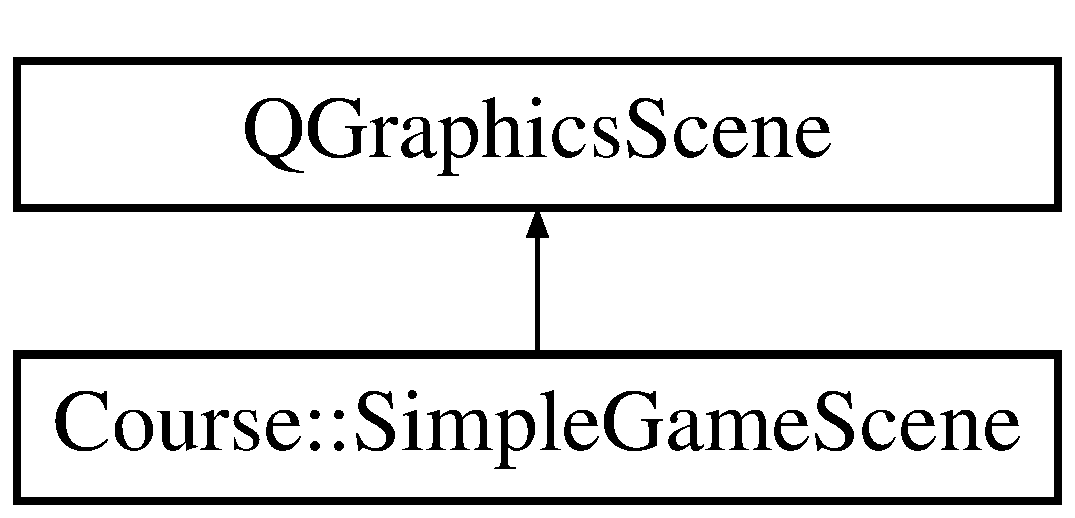
\includegraphics[height=2.000000cm]{classCourse_1_1SimpleGameScene}
\end{center}
\end{figure}
\subsection*{Signals}
\begin{DoxyCompactItemize}
\item 
void \hyperlink{classCourse_1_1SimpleGameScene_ad589e26e037e1915fc8d4c0f06140a01}{object\-Clicked} (unsigned int object\-\_\-id)
\end{DoxyCompactItemize}
\subsection*{Public Member Functions}
\begin{DoxyCompactItemize}
\item 
\hyperlink{classCourse_1_1SimpleGameScene_ae65dfd293c3490dcbb71d7a71ddda65b}{Simple\-Game\-Scene} (Q\-Widget $\ast$qt\-\_\-parent=nullptr, int width=10, int height=10, int scale=50)
\begin{DoxyCompactList}\small\item\em Constructor for the class. \end{DoxyCompactList}\item 
\hyperlink{classCourse_1_1SimpleGameScene_ab8addb19d78f539947e163d7ec37e49c}{$\sim$\-Simple\-Game\-Scene} ()=default
\begin{DoxyCompactList}\small\item\em Default destructor. \end{DoxyCompactList}\item 
void \hyperlink{classCourse_1_1SimpleGameScene_a418450a3659d632ff3ba0696ffe88adc}{set\-Size} (int width, int height)
\begin{DoxyCompactList}\small\item\em Sets the map size and calls \hyperlink{classCourse_1_1SimpleGameScene_a2a097ef678bc2eaabe93832917d2aedf}{resize()}. \end{DoxyCompactList}\item 
void \hyperlink{classCourse_1_1SimpleGameScene_a97c12ca31ae67a45b5cf3e53065c5631}{set\-Scale} (int scale)
\begin{DoxyCompactList}\small\item\em set the tile size, aka scale of the map and calls \hyperlink{classCourse_1_1SimpleGameScene_a2a097ef678bc2eaabe93832917d2aedf}{resize()}. Function behaviour after objects has been drawn is not specified. \end{DoxyCompactList}\item 
void \hyperlink{classCourse_1_1SimpleGameScene_a2a097ef678bc2eaabe93832917d2aedf}{resize} ()
\begin{DoxyCompactList}\small\item\em resize recalculates the bounding rectangle \end{DoxyCompactList}\item 
int \hyperlink{classCourse_1_1SimpleGameScene_aefad6eb4433f9e89850e96697b980831}{get\-Scale} () const 
\begin{DoxyCompactList}\small\item\em get the size of a single tile \end{DoxyCompactList}\item 
std\-::pair$<$ int, int $>$ \hyperlink{classCourse_1_1SimpleGameScene_a47bac76decd9c47bb4604a7f0c2d6de7}{get\-Size} () const 
\begin{DoxyCompactList}\small\item\em get the size of the map. \end{DoxyCompactList}\item 
void \hyperlink{classCourse_1_1SimpleGameScene_adc6d386caaf44e3ef33a266f46e7eb98}{draw\-Item} (std\-::shared\-\_\-ptr$<$ \hyperlink{classCourse_1_1GameObject}{Course\-::\-Game\-Object} $>$ obj)
\begin{DoxyCompactList}\small\item\em draw a new item to the map. \end{DoxyCompactList}\item 
void \hyperlink{classCourse_1_1SimpleGameScene_a9184f8347367a255ddb9a1b0ce23e134}{remove\-Item} (std\-::shared\-\_\-ptr$<$ \hyperlink{classCourse_1_1GameObject}{Course\-::\-Game\-Object} $>$ obj)
\begin{DoxyCompactList}\small\item\em tries to remove drawn object at the location obj points to. If there's multiple objects, will remove the one that matches obj. \end{DoxyCompactList}\item 
void \hyperlink{classCourse_1_1SimpleGameScene_ae175f970177c7564b6fb63f8869a44e3}{update\-Item} (std\-::shared\-\_\-ptr$<$ \hyperlink{classCourse_1_1GameObject}{Course\-::\-Game\-Object} $>$ obj)
\begin{DoxyCompactList}\small\item\em updates the position of obj. \end{DoxyCompactList}\item 
virtual bool \hyperlink{classCourse_1_1SimpleGameScene_a8853ddab78ee57fe69489cb246c2dcad}{event} (Q\-Event $\ast$event) override
\begin{DoxyCompactList}\small\item\em simple event handler that notifies when objects or the play area is clicked. \end{DoxyCompactList}\end{DoxyCompactItemize}
\subsection*{Private Attributes}
\begin{DoxyCompactItemize}
\item 
Q\-Graphics\-Item $\ast$ \hyperlink{classCourse_1_1SimpleGameScene_a0fb914c9a9a0b0f609a8e37122dfc66b}{m\-\_\-map\-Bound\-Rect}
\item 
int \hyperlink{classCourse_1_1SimpleGameScene_a092cd06906c5f7bf90932155cce61c65}{m\-\_\-width}
\item 
int \hyperlink{classCourse_1_1SimpleGameScene_ab9f181b61998050f4705136d4b8ac037}{m\-\_\-height}
\item 
int \hyperlink{classCourse_1_1SimpleGameScene_abcfe6adc631563891c7400147bb9de3f}{m\-\_\-scale}
\end{DoxyCompactItemize}


\subsection{Detailed Description}
The \hyperlink{classCourse_1_1SimpleGameScene}{Simple\-Game\-Scene} is a custom Q\-Graphics\-Scene that shows a simple rendering of the game map. 

\subsection{Constructor \& Destructor Documentation}
\hypertarget{classCourse_1_1SimpleGameScene_ae65dfd293c3490dcbb71d7a71ddda65b}{\index{Course\-::\-Simple\-Game\-Scene@{Course\-::\-Simple\-Game\-Scene}!Simple\-Game\-Scene@{Simple\-Game\-Scene}}
\index{Simple\-Game\-Scene@{Simple\-Game\-Scene}!Course::SimpleGameScene@{Course\-::\-Simple\-Game\-Scene}}
\subsubsection[{Simple\-Game\-Scene}]{\setlength{\rightskip}{0pt plus 5cm}Course\-::\-Simple\-Game\-Scene\-::\-Simple\-Game\-Scene (
\begin{DoxyParamCaption}
\item[{Q\-Widget $\ast$}]{qt\-\_\-parent = {\ttfamily nullptr}, }
\item[{int}]{width = {\ttfamily 10}, }
\item[{int}]{height = {\ttfamily 10}, }
\item[{int}]{scale = {\ttfamily 50}}
\end{DoxyParamCaption}
)}}\label{classCourse_1_1SimpleGameScene_ae65dfd293c3490dcbb71d7a71ddda65b}


Constructor for the class. 


\begin{DoxyParams}{Parameters}
{\em qt\-\_\-parent} & points to the parent object per Qt's parent-\/child-\/system. \\
\hline
{\em width} & in tiles for the game map. \\
\hline
{\em height} & in tiles for the game map. \\
\hline
{\em scale} & is the size in pixels of a single square tile.\\
\hline
\end{DoxyParams}
\begin{DoxyPrecond}{Precondition}
0 $<$ width $<$= 100 \&\& 0 $<$ height $<$= 100 \&\& 0 $<$ scale $<$= 500. Otherwise default values are used for the created object. 
\end{DoxyPrecond}
\hypertarget{classCourse_1_1SimpleGameScene_ab8addb19d78f539947e163d7ec37e49c}{\index{Course\-::\-Simple\-Game\-Scene@{Course\-::\-Simple\-Game\-Scene}!$\sim$\-Simple\-Game\-Scene@{$\sim$\-Simple\-Game\-Scene}}
\index{$\sim$\-Simple\-Game\-Scene@{$\sim$\-Simple\-Game\-Scene}!Course::SimpleGameScene@{Course\-::\-Simple\-Game\-Scene}}
\subsubsection[{$\sim$\-Simple\-Game\-Scene}]{\setlength{\rightskip}{0pt plus 5cm}Course\-::\-Simple\-Game\-Scene\-::$\sim$\-Simple\-Game\-Scene (
\begin{DoxyParamCaption}
{}
\end{DoxyParamCaption}
)\hspace{0.3cm}{\ttfamily [default]}}}\label{classCourse_1_1SimpleGameScene_ab8addb19d78f539947e163d7ec37e49c}


Default destructor. 



\subsection{Member Function Documentation}
\hypertarget{classCourse_1_1SimpleGameScene_adc6d386caaf44e3ef33a266f46e7eb98}{\index{Course\-::\-Simple\-Game\-Scene@{Course\-::\-Simple\-Game\-Scene}!draw\-Item@{draw\-Item}}
\index{draw\-Item@{draw\-Item}!Course::SimpleGameScene@{Course\-::\-Simple\-Game\-Scene}}
\subsubsection[{draw\-Item}]{\setlength{\rightskip}{0pt plus 5cm}void Course\-::\-Simple\-Game\-Scene\-::draw\-Item (
\begin{DoxyParamCaption}
\item[{std\-::shared\-\_\-ptr$<$ {\bf Course\-::\-Game\-Object} $>$}]{obj}
\end{DoxyParamCaption}
)}}\label{classCourse_1_1SimpleGameScene_adc6d386caaf44e3ef33a266f46e7eb98}


draw a new item to the map. 


\begin{DoxyParams}{Parameters}
{\em obj} & shared ptr to the object \\
\hline
\end{DoxyParams}
\begin{DoxyPrecond}{Precondition}
obj must have a valid coordinate property. 
\end{DoxyPrecond}
\begin{DoxyPostcond}{Postcondition}
Exception guarantee\-: None 
\end{DoxyPostcond}
\hypertarget{classCourse_1_1SimpleGameScene_a8853ddab78ee57fe69489cb246c2dcad}{\index{Course\-::\-Simple\-Game\-Scene@{Course\-::\-Simple\-Game\-Scene}!event@{event}}
\index{event@{event}!Course::SimpleGameScene@{Course\-::\-Simple\-Game\-Scene}}
\subsubsection[{event}]{\setlength{\rightskip}{0pt plus 5cm}bool Course\-::\-Simple\-Game\-Scene\-::event (
\begin{DoxyParamCaption}
\item[{Q\-Event $\ast$}]{event}
\end{DoxyParamCaption}
)\hspace{0.3cm}{\ttfamily [override]}, {\ttfamily [virtual]}}}\label{classCourse_1_1SimpleGameScene_a8853ddab78ee57fe69489cb246c2dcad}


simple event handler that notifies when objects or the play area is clicked. 


\begin{DoxyParams}{Parameters}
{\em event} & that has happened. \\
\hline
\end{DoxyParams}
\begin{DoxyReturn}{Returns}
True\-: if event was handled in the handler. False\-: if the event handling was passed over. 
\end{DoxyReturn}
\hypertarget{classCourse_1_1SimpleGameScene_aefad6eb4433f9e89850e96697b980831}{\index{Course\-::\-Simple\-Game\-Scene@{Course\-::\-Simple\-Game\-Scene}!get\-Scale@{get\-Scale}}
\index{get\-Scale@{get\-Scale}!Course::SimpleGameScene@{Course\-::\-Simple\-Game\-Scene}}
\subsubsection[{get\-Scale}]{\setlength{\rightskip}{0pt plus 5cm}int Course\-::\-Simple\-Game\-Scene\-::get\-Scale (
\begin{DoxyParamCaption}
{}
\end{DoxyParamCaption}
) const}}\label{classCourse_1_1SimpleGameScene_aefad6eb4433f9e89850e96697b980831}


get the size of a single tile 

\begin{DoxyReturn}{Returns}
the size of a tile in pixels. 
\end{DoxyReturn}
\begin{DoxyPostcond}{Postcondition}
Exception guarantee\-: No-\/throw 
\end{DoxyPostcond}
\hypertarget{classCourse_1_1SimpleGameScene_a47bac76decd9c47bb4604a7f0c2d6de7}{\index{Course\-::\-Simple\-Game\-Scene@{Course\-::\-Simple\-Game\-Scene}!get\-Size@{get\-Size}}
\index{get\-Size@{get\-Size}!Course::SimpleGameScene@{Course\-::\-Simple\-Game\-Scene}}
\subsubsection[{get\-Size}]{\setlength{\rightskip}{0pt plus 5cm}std\-::pair$<$ int, int $>$ Course\-::\-Simple\-Game\-Scene\-::get\-Size (
\begin{DoxyParamCaption}
{}
\end{DoxyParamCaption}
) const}}\label{classCourse_1_1SimpleGameScene_a47bac76decd9c47bb4604a7f0c2d6de7}


get the size of the map. 

\begin{DoxyReturn}{Returns}
pair$<$width, height$>$ in tiles. 
\end{DoxyReturn}
\begin{DoxyPostcond}{Postcondition}
Exception guarantee\-: No-\/throw 
\end{DoxyPostcond}
\hypertarget{classCourse_1_1SimpleGameScene_ad589e26e037e1915fc8d4c0f06140a01}{\index{Course\-::\-Simple\-Game\-Scene@{Course\-::\-Simple\-Game\-Scene}!object\-Clicked@{object\-Clicked}}
\index{object\-Clicked@{object\-Clicked}!Course::SimpleGameScene@{Course\-::\-Simple\-Game\-Scene}}
\subsubsection[{object\-Clicked}]{\setlength{\rightskip}{0pt plus 5cm}void Course\-::\-Simple\-Game\-Scene\-::object\-Clicked (
\begin{DoxyParamCaption}
\item[{unsigned int}]{object\-\_\-id}
\end{DoxyParamCaption}
)\hspace{0.3cm}{\ttfamily [signal]}}}\label{classCourse_1_1SimpleGameScene_ad589e26e037e1915fc8d4c0f06140a01}
\hypertarget{classCourse_1_1SimpleGameScene_a9184f8347367a255ddb9a1b0ce23e134}{\index{Course\-::\-Simple\-Game\-Scene@{Course\-::\-Simple\-Game\-Scene}!remove\-Item@{remove\-Item}}
\index{remove\-Item@{remove\-Item}!Course::SimpleGameScene@{Course\-::\-Simple\-Game\-Scene}}
\subsubsection[{remove\-Item}]{\setlength{\rightskip}{0pt plus 5cm}void Course\-::\-Simple\-Game\-Scene\-::remove\-Item (
\begin{DoxyParamCaption}
\item[{std\-::shared\-\_\-ptr$<$ {\bf Course\-::\-Game\-Object} $>$}]{obj}
\end{DoxyParamCaption}
)}}\label{classCourse_1_1SimpleGameScene_a9184f8347367a255ddb9a1b0ce23e134}


tries to remove drawn object at the location obj points to. If there's multiple objects, will remove the one that matches obj. 


\begin{DoxyParams}{Parameters}
{\em obj} & shared ptr to the object being deleted. \\
\hline
\end{DoxyParams}
\begin{DoxyPostcond}{Postcondition}
Exception guarantee\-: None 
\end{DoxyPostcond}
\hypertarget{classCourse_1_1SimpleGameScene_a2a097ef678bc2eaabe93832917d2aedf}{\index{Course\-::\-Simple\-Game\-Scene@{Course\-::\-Simple\-Game\-Scene}!resize@{resize}}
\index{resize@{resize}!Course::SimpleGameScene@{Course\-::\-Simple\-Game\-Scene}}
\subsubsection[{resize}]{\setlength{\rightskip}{0pt plus 5cm}void Course\-::\-Simple\-Game\-Scene\-::resize (
\begin{DoxyParamCaption}
{}
\end{DoxyParamCaption}
)}}\label{classCourse_1_1SimpleGameScene_a2a097ef678bc2eaabe93832917d2aedf}


resize recalculates the bounding rectangle 

\hypertarget{classCourse_1_1SimpleGameScene_a97c12ca31ae67a45b5cf3e53065c5631}{\index{Course\-::\-Simple\-Game\-Scene@{Course\-::\-Simple\-Game\-Scene}!set\-Scale@{set\-Scale}}
\index{set\-Scale@{set\-Scale}!Course::SimpleGameScene@{Course\-::\-Simple\-Game\-Scene}}
\subsubsection[{set\-Scale}]{\setlength{\rightskip}{0pt plus 5cm}void Course\-::\-Simple\-Game\-Scene\-::set\-Scale (
\begin{DoxyParamCaption}
\item[{int}]{scale}
\end{DoxyParamCaption}
)}}\label{classCourse_1_1SimpleGameScene_a97c12ca31ae67a45b5cf3e53065c5631}


set the tile size, aka scale of the map and calls \hyperlink{classCourse_1_1SimpleGameScene_a2a097ef678bc2eaabe93832917d2aedf}{resize()}. Function behaviour after objects has been drawn is not specified. 


\begin{DoxyParams}{Parameters}
{\em scale} & in pixels. \\
\hline
\end{DoxyParams}
\begin{DoxyPrecond}{Precondition}
0 $<$ scale $<$= 500 
\end{DoxyPrecond}
\begin{DoxyPostcond}{Postcondition}
Scene scale is set to scale. 

Exception guarantee\-: None 
\end{DoxyPostcond}
\hypertarget{classCourse_1_1SimpleGameScene_a418450a3659d632ff3ba0696ffe88adc}{\index{Course\-::\-Simple\-Game\-Scene@{Course\-::\-Simple\-Game\-Scene}!set\-Size@{set\-Size}}
\index{set\-Size@{set\-Size}!Course::SimpleGameScene@{Course\-::\-Simple\-Game\-Scene}}
\subsubsection[{set\-Size}]{\setlength{\rightskip}{0pt plus 5cm}void Course\-::\-Simple\-Game\-Scene\-::set\-Size (
\begin{DoxyParamCaption}
\item[{int}]{width, }
\item[{int}]{height}
\end{DoxyParamCaption}
)}}\label{classCourse_1_1SimpleGameScene_a418450a3659d632ff3ba0696ffe88adc}


Sets the map size and calls \hyperlink{classCourse_1_1SimpleGameScene_a2a097ef678bc2eaabe93832917d2aedf}{resize()}. 


\begin{DoxyParams}{Parameters}
{\em width} & in tiles. \\
\hline
{\em height} & in tiles. \\
\hline
\end{DoxyParams}
\begin{DoxyPrecond}{Precondition}
width and height must each be between 1 and 100. 
\end{DoxyPrecond}
\begin{DoxyPostcond}{Postcondition}
width and height are set to given sizes. 

Exception guarantee\-: No-\/throw 
\end{DoxyPostcond}
\hypertarget{classCourse_1_1SimpleGameScene_ae175f970177c7564b6fb63f8869a44e3}{\index{Course\-::\-Simple\-Game\-Scene@{Course\-::\-Simple\-Game\-Scene}!update\-Item@{update\-Item}}
\index{update\-Item@{update\-Item}!Course::SimpleGameScene@{Course\-::\-Simple\-Game\-Scene}}
\subsubsection[{update\-Item}]{\setlength{\rightskip}{0pt plus 5cm}void Course\-::\-Simple\-Game\-Scene\-::update\-Item (
\begin{DoxyParamCaption}
\item[{std\-::shared\-\_\-ptr$<$ {\bf Course\-::\-Game\-Object} $>$}]{obj}
\end{DoxyParamCaption}
)}}\label{classCourse_1_1SimpleGameScene_ae175f970177c7564b6fb63f8869a44e3}


updates the position of obj. 


\begin{DoxyParams}{Parameters}
{\em obj} & shared ptr to the obj being updated. \\
\hline
\end{DoxyParams}


\subsection{Member Data Documentation}
\hypertarget{classCourse_1_1SimpleGameScene_ab9f181b61998050f4705136d4b8ac037}{\index{Course\-::\-Simple\-Game\-Scene@{Course\-::\-Simple\-Game\-Scene}!m\-\_\-height@{m\-\_\-height}}
\index{m\-\_\-height@{m\-\_\-height}!Course::SimpleGameScene@{Course\-::\-Simple\-Game\-Scene}}
\subsubsection[{m\-\_\-height}]{\setlength{\rightskip}{0pt plus 5cm}int Course\-::\-Simple\-Game\-Scene\-::m\-\_\-height\hspace{0.3cm}{\ttfamily [private]}}}\label{classCourse_1_1SimpleGameScene_ab9f181b61998050f4705136d4b8ac037}
\hypertarget{classCourse_1_1SimpleGameScene_a0fb914c9a9a0b0f609a8e37122dfc66b}{\index{Course\-::\-Simple\-Game\-Scene@{Course\-::\-Simple\-Game\-Scene}!m\-\_\-map\-Bound\-Rect@{m\-\_\-map\-Bound\-Rect}}
\index{m\-\_\-map\-Bound\-Rect@{m\-\_\-map\-Bound\-Rect}!Course::SimpleGameScene@{Course\-::\-Simple\-Game\-Scene}}
\subsubsection[{m\-\_\-map\-Bound\-Rect}]{\setlength{\rightskip}{0pt plus 5cm}Q\-Graphics\-Item$\ast$ Course\-::\-Simple\-Game\-Scene\-::m\-\_\-map\-Bound\-Rect\hspace{0.3cm}{\ttfamily [private]}}}\label{classCourse_1_1SimpleGameScene_a0fb914c9a9a0b0f609a8e37122dfc66b}
\hypertarget{classCourse_1_1SimpleGameScene_abcfe6adc631563891c7400147bb9de3f}{\index{Course\-::\-Simple\-Game\-Scene@{Course\-::\-Simple\-Game\-Scene}!m\-\_\-scale@{m\-\_\-scale}}
\index{m\-\_\-scale@{m\-\_\-scale}!Course::SimpleGameScene@{Course\-::\-Simple\-Game\-Scene}}
\subsubsection[{m\-\_\-scale}]{\setlength{\rightskip}{0pt plus 5cm}int Course\-::\-Simple\-Game\-Scene\-::m\-\_\-scale\hspace{0.3cm}{\ttfamily [private]}}}\label{classCourse_1_1SimpleGameScene_abcfe6adc631563891c7400147bb9de3f}
\hypertarget{classCourse_1_1SimpleGameScene_a092cd06906c5f7bf90932155cce61c65}{\index{Course\-::\-Simple\-Game\-Scene@{Course\-::\-Simple\-Game\-Scene}!m\-\_\-width@{m\-\_\-width}}
\index{m\-\_\-width@{m\-\_\-width}!Course::SimpleGameScene@{Course\-::\-Simple\-Game\-Scene}}
\subsubsection[{m\-\_\-width}]{\setlength{\rightskip}{0pt plus 5cm}int Course\-::\-Simple\-Game\-Scene\-::m\-\_\-width\hspace{0.3cm}{\ttfamily [private]}}}\label{classCourse_1_1SimpleGameScene_a092cd06906c5f7bf90932155cce61c65}


The documentation for this class was generated from the following files\-:\begin{DoxyCompactItemize}
\item 
Course/\-Course\-Lib/graphics/\hyperlink{simplegamescene_8h}{simplegamescene.\-h}\item 
Course/\-Course\-Lib/graphics/\hyperlink{simplegamescene_8cpp}{simplegamescene.\-cpp}\end{DoxyCompactItemize}

\hypertarget{classCourse_1_1SimpleMapItem}{\section{Course\-:\-:Simple\-Map\-Item Class Reference}
\label{classCourse_1_1SimpleMapItem}\index{Course\-::\-Simple\-Map\-Item@{Course\-::\-Simple\-Map\-Item}}
}


The \hyperlink{classCourse_1_1SimpleMapItem}{Simple\-Map\-Item} class is a custom Q\-Graphics\-Item that acts as a single \hyperlink{classCourse_1_1GameObject}{Game\-Object}'s graphical element.  




{\ttfamily \#include $<$simplemapitem.\-h$>$}

Inheritance diagram for Course\-:\-:Simple\-Map\-Item\-:\begin{figure}[H]
\begin{center}
\leavevmode
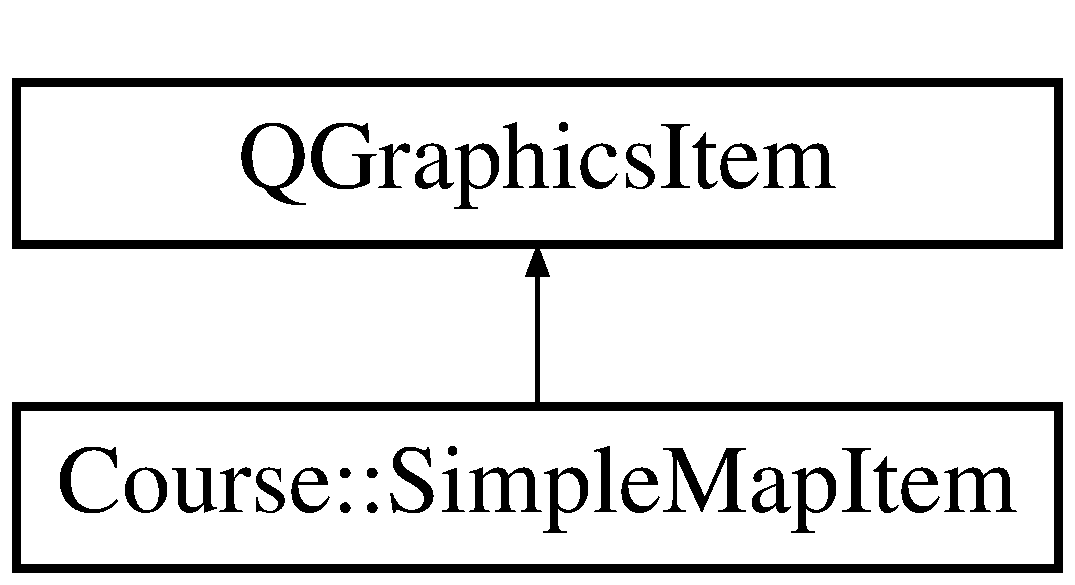
\includegraphics[height=2.000000cm]{classCourse_1_1SimpleMapItem}
\end{center}
\end{figure}
\subsection*{Public Member Functions}
\begin{DoxyCompactItemize}
\item 
\hyperlink{classCourse_1_1SimpleMapItem_a3203bf5f513161593f4036320b7c24c6}{Simple\-Map\-Item} (const std\-::shared\-\_\-ptr$<$ \hyperlink{classCourse_1_1GameObject}{Course\-::\-Game\-Object} $>$ \&obj, int size)
\begin{DoxyCompactList}\small\item\em Constructor. \end{DoxyCompactList}\item 
Q\-Rect\-F \hyperlink{classCourse_1_1SimpleMapItem_ad103986c7b67b3e1c69e10291e6c4b36}{bounding\-Rect} () const override
\begin{DoxyCompactList}\small\item\em bounding\-Rect \end{DoxyCompactList}\item 
void \hyperlink{classCourse_1_1SimpleMapItem_a42f0b7bd86da05bcc511486362aabb8b}{paint} (Q\-Painter $\ast$painter, const Q\-Style\-Option\-Graphics\-Item $\ast$option, Q\-Widget $\ast$widget)
\begin{DoxyCompactList}\small\item\em paints the item \end{DoxyCompactList}\item 
const std\-::shared\-\_\-ptr\\*
$<$ \hyperlink{classCourse_1_1GameObject}{Course\-::\-Game\-Object} $>$ \& \hyperlink{classCourse_1_1SimpleMapItem_ad244bfbca3b53ec888ae7fa07b004e68}{get\-Bound\-Object} ()
\begin{DoxyCompactList}\small\item\em get\-Bound\-Object \end{DoxyCompactList}\item 
void \hyperlink{classCourse_1_1SimpleMapItem_a7b064cd8193aff3a1e810582e9e75786}{update\-Loc} ()
\begin{DoxyCompactList}\small\item\em update\-Loc moves the item if the position has changed. \end{DoxyCompactList}\item 
bool \hyperlink{classCourse_1_1SimpleMapItem_a95cc703e4962903f3a67bee4eb7c7165}{is\-Same\-Obj} (std\-::shared\-\_\-ptr$<$ \hyperlink{classCourse_1_1GameObject}{Course\-::\-Game\-Object} $>$ obj)
\begin{DoxyCompactList}\small\item\em checks if this instance has obj as bound obj. \end{DoxyCompactList}\item 
int \hyperlink{classCourse_1_1SimpleMapItem_af80e162edd2c57e5f74b88cdc8113721}{get\-Size} () const 
\begin{DoxyCompactList}\small\item\em get\-Size \end{DoxyCompactList}\item 
void \hyperlink{classCourse_1_1SimpleMapItem_aaff1ad6f7daac8b91bb606d9d2b26f4a}{set\-Size} (int size)
\begin{DoxyCompactList}\small\item\em set\-Size \end{DoxyCompactList}\end{DoxyCompactItemize}
\subsection*{Static Private Member Functions}
\begin{DoxyCompactItemize}
\item 
static void \hyperlink{classCourse_1_1SimpleMapItem_ae00337284799adff891f10d4ec1396d5}{add\-New\-Color} (std\-::string type)
\end{DoxyCompactItemize}
\subsection*{Private Attributes}
\begin{DoxyCompactItemize}
\item 
const std\-::shared\-\_\-ptr\\*
$<$ \hyperlink{classCourse_1_1GameObject}{Course\-::\-Game\-Object} $>$ \hyperlink{classCourse_1_1SimpleMapItem_a4e067b04d171bb5e0a74f0f9c6419e95}{m\-\_\-gameobject}
\item 
Q\-Point \hyperlink{classCourse_1_1SimpleMapItem_a23c29a1b2a650ea0d9e5f7c1cc9a28f3}{m\-\_\-scenelocation}
\item 
int \hyperlink{classCourse_1_1SimpleMapItem_a68703106114f279f0fa103057d4b77af}{m\-\_\-size}
\end{DoxyCompactItemize}
\subsection*{Static Private Attributes}
\begin{DoxyCompactItemize}
\item 
static std\-::map$<$ std\-::string, \\*
Q\-Color $>$ \hyperlink{classCourse_1_1SimpleMapItem_adf954f1c53a9651e2634cd307be9aab4}{c\-\_\-mapcolors} = \{\}
\end{DoxyCompactItemize}


\subsection{Detailed Description}
The \hyperlink{classCourse_1_1SimpleMapItem}{Simple\-Map\-Item} class is a custom Q\-Graphics\-Item that acts as a single \hyperlink{classCourse_1_1GameObject}{Game\-Object}'s graphical element. 

\subsection{Constructor \& Destructor Documentation}
\hypertarget{classCourse_1_1SimpleMapItem_a3203bf5f513161593f4036320b7c24c6}{\index{Course\-::\-Simple\-Map\-Item@{Course\-::\-Simple\-Map\-Item}!Simple\-Map\-Item@{Simple\-Map\-Item}}
\index{Simple\-Map\-Item@{Simple\-Map\-Item}!Course::SimpleMapItem@{Course\-::\-Simple\-Map\-Item}}
\subsubsection[{Simple\-Map\-Item}]{\setlength{\rightskip}{0pt plus 5cm}Course\-::\-Simple\-Map\-Item\-::\-Simple\-Map\-Item (
\begin{DoxyParamCaption}
\item[{const std\-::shared\-\_\-ptr$<$ {\bf Course\-::\-Game\-Object} $>$ \&}]{obj, }
\item[{int}]{size}
\end{DoxyParamCaption}
)}}\label{classCourse_1_1SimpleMapItem_a3203bf5f513161593f4036320b7c24c6}


Constructor. 


\begin{DoxyParams}{Parameters}
{\em obj} & shared\-\_\-ptr to the obj. \\
\hline
{\em size} & of the created item in pixels. \\
\hline
\end{DoxyParams}
\begin{DoxyPrecond}{Precondition}
obj must have a valid \hyperlink{classCourse_1_1Coordinate}{Coordinate}. 
\end{DoxyPrecond}


\subsection{Member Function Documentation}
\hypertarget{classCourse_1_1SimpleMapItem_ae00337284799adff891f10d4ec1396d5}{\index{Course\-::\-Simple\-Map\-Item@{Course\-::\-Simple\-Map\-Item}!add\-New\-Color@{add\-New\-Color}}
\index{add\-New\-Color@{add\-New\-Color}!Course::SimpleMapItem@{Course\-::\-Simple\-Map\-Item}}
\subsubsection[{add\-New\-Color}]{\setlength{\rightskip}{0pt plus 5cm}void Course\-::\-Simple\-Map\-Item\-::add\-New\-Color (
\begin{DoxyParamCaption}
\item[{std\-::string}]{type}
\end{DoxyParamCaption}
)\hspace{0.3cm}{\ttfamily [static]}, {\ttfamily [private]}}}\label{classCourse_1_1SimpleMapItem_ae00337284799adff891f10d4ec1396d5}
\hypertarget{classCourse_1_1SimpleMapItem_ad103986c7b67b3e1c69e10291e6c4b36}{\index{Course\-::\-Simple\-Map\-Item@{Course\-::\-Simple\-Map\-Item}!bounding\-Rect@{bounding\-Rect}}
\index{bounding\-Rect@{bounding\-Rect}!Course::SimpleMapItem@{Course\-::\-Simple\-Map\-Item}}
\subsubsection[{bounding\-Rect}]{\setlength{\rightskip}{0pt plus 5cm}Q\-Rect\-F Course\-::\-Simple\-Map\-Item\-::bounding\-Rect (
\begin{DoxyParamCaption}
{}
\end{DoxyParamCaption}
) const\hspace{0.3cm}{\ttfamily [override]}}}\label{classCourse_1_1SimpleMapItem_ad103986c7b67b3e1c69e10291e6c4b36}


bounding\-Rect 

\begin{DoxyReturn}{Returns}
the bounding rectangle of this item. 
\end{DoxyReturn}
\hypertarget{classCourse_1_1SimpleMapItem_ad244bfbca3b53ec888ae7fa07b004e68}{\index{Course\-::\-Simple\-Map\-Item@{Course\-::\-Simple\-Map\-Item}!get\-Bound\-Object@{get\-Bound\-Object}}
\index{get\-Bound\-Object@{get\-Bound\-Object}!Course::SimpleMapItem@{Course\-::\-Simple\-Map\-Item}}
\subsubsection[{get\-Bound\-Object}]{\setlength{\rightskip}{0pt plus 5cm}const std\-::shared\-\_\-ptr$<$ {\bf Course\-::\-Game\-Object} $>$ \& Course\-::\-Simple\-Map\-Item\-::get\-Bound\-Object (
\begin{DoxyParamCaption}
{}
\end{DoxyParamCaption}
)}}\label{classCourse_1_1SimpleMapItem_ad244bfbca3b53ec888ae7fa07b004e68}


get\-Bound\-Object 

\begin{DoxyReturn}{Returns}
the object this item is bound to. 
\end{DoxyReturn}
\hypertarget{classCourse_1_1SimpleMapItem_af80e162edd2c57e5f74b88cdc8113721}{\index{Course\-::\-Simple\-Map\-Item@{Course\-::\-Simple\-Map\-Item}!get\-Size@{get\-Size}}
\index{get\-Size@{get\-Size}!Course::SimpleMapItem@{Course\-::\-Simple\-Map\-Item}}
\subsubsection[{get\-Size}]{\setlength{\rightskip}{0pt plus 5cm}int Course\-::\-Simple\-Map\-Item\-::get\-Size (
\begin{DoxyParamCaption}
{}
\end{DoxyParamCaption}
) const}}\label{classCourse_1_1SimpleMapItem_af80e162edd2c57e5f74b88cdc8113721}


get\-Size 

\begin{DoxyReturn}{Returns}
size of the object in pixels. 
\end{DoxyReturn}
\begin{DoxyPostcond}{Postcondition}
Exception guarantee\-: No-\/throw 
\end{DoxyPostcond}
\hypertarget{classCourse_1_1SimpleMapItem_a95cc703e4962903f3a67bee4eb7c7165}{\index{Course\-::\-Simple\-Map\-Item@{Course\-::\-Simple\-Map\-Item}!is\-Same\-Obj@{is\-Same\-Obj}}
\index{is\-Same\-Obj@{is\-Same\-Obj}!Course::SimpleMapItem@{Course\-::\-Simple\-Map\-Item}}
\subsubsection[{is\-Same\-Obj}]{\setlength{\rightskip}{0pt plus 5cm}bool Course\-::\-Simple\-Map\-Item\-::is\-Same\-Obj (
\begin{DoxyParamCaption}
\item[{std\-::shared\-\_\-ptr$<$ {\bf Course\-::\-Game\-Object} $>$}]{obj}
\end{DoxyParamCaption}
)}}\label{classCourse_1_1SimpleMapItem_a95cc703e4962903f3a67bee4eb7c7165}


checks if this instance has obj as bound obj. 


\begin{DoxyParams}{Parameters}
{\em obj} & to compare to. \\
\hline
\end{DoxyParams}
\begin{DoxyReturn}{Returns}
True\-: if obj is pointing to the same object as this item. False otherwise. 
\end{DoxyReturn}
\hypertarget{classCourse_1_1SimpleMapItem_a42f0b7bd86da05bcc511486362aabb8b}{\index{Course\-::\-Simple\-Map\-Item@{Course\-::\-Simple\-Map\-Item}!paint@{paint}}
\index{paint@{paint}!Course::SimpleMapItem@{Course\-::\-Simple\-Map\-Item}}
\subsubsection[{paint}]{\setlength{\rightskip}{0pt plus 5cm}void Course\-::\-Simple\-Map\-Item\-::paint (
\begin{DoxyParamCaption}
\item[{Q\-Painter $\ast$}]{painter, }
\item[{const Q\-Style\-Option\-Graphics\-Item $\ast$}]{option, }
\item[{Q\-Widget $\ast$}]{widget}
\end{DoxyParamCaption}
)}}\label{classCourse_1_1SimpleMapItem_a42f0b7bd86da05bcc511486362aabb8b}


paints the item 


\begin{DoxyParams}{Parameters}
{\em painter} & \\
\hline
{\em option} & \\
\hline
{\em widget} & \\
\hline
\end{DoxyParams}
\begin{DoxyNote}{Note}
The Graphics\-View containing the scene this belongs to usually calls this function. 
\end{DoxyNote}
\hypertarget{classCourse_1_1SimpleMapItem_aaff1ad6f7daac8b91bb606d9d2b26f4a}{\index{Course\-::\-Simple\-Map\-Item@{Course\-::\-Simple\-Map\-Item}!set\-Size@{set\-Size}}
\index{set\-Size@{set\-Size}!Course::SimpleMapItem@{Course\-::\-Simple\-Map\-Item}}
\subsubsection[{set\-Size}]{\setlength{\rightskip}{0pt plus 5cm}void Course\-::\-Simple\-Map\-Item\-::set\-Size (
\begin{DoxyParamCaption}
\item[{int}]{size}
\end{DoxyParamCaption}
)}}\label{classCourse_1_1SimpleMapItem_aaff1ad6f7daac8b91bb606d9d2b26f4a}


set\-Size 


\begin{DoxyParams}{Parameters}
{\em size} & of the object in pixels. \\
\hline
\end{DoxyParams}
\begin{DoxyPrecond}{Precondition}
0 $<$ size $<$= 500 
\end{DoxyPrecond}
\begin{DoxyPostcond}{Postcondition}
Exception guarantee\-: No-\/throw 
\end{DoxyPostcond}
\hypertarget{classCourse_1_1SimpleMapItem_a7b064cd8193aff3a1e810582e9e75786}{\index{Course\-::\-Simple\-Map\-Item@{Course\-::\-Simple\-Map\-Item}!update\-Loc@{update\-Loc}}
\index{update\-Loc@{update\-Loc}!Course::SimpleMapItem@{Course\-::\-Simple\-Map\-Item}}
\subsubsection[{update\-Loc}]{\setlength{\rightskip}{0pt plus 5cm}void Course\-::\-Simple\-Map\-Item\-::update\-Loc (
\begin{DoxyParamCaption}
{}
\end{DoxyParamCaption}
)}}\label{classCourse_1_1SimpleMapItem_a7b064cd8193aff3a1e810582e9e75786}


update\-Loc moves the item if the position has changed. 



\subsection{Member Data Documentation}
\hypertarget{classCourse_1_1SimpleMapItem_adf954f1c53a9651e2634cd307be9aab4}{\index{Course\-::\-Simple\-Map\-Item@{Course\-::\-Simple\-Map\-Item}!c\-\_\-mapcolors@{c\-\_\-mapcolors}}
\index{c\-\_\-mapcolors@{c\-\_\-mapcolors}!Course::SimpleMapItem@{Course\-::\-Simple\-Map\-Item}}
\subsubsection[{c\-\_\-mapcolors}]{\setlength{\rightskip}{0pt plus 5cm}std\-::map$<$ std\-::string, Q\-Color $>$ Course\-::\-Simple\-Map\-Item\-::c\-\_\-mapcolors = \{\}\hspace{0.3cm}{\ttfamily [static]}, {\ttfamily [private]}}}\label{classCourse_1_1SimpleMapItem_adf954f1c53a9651e2634cd307be9aab4}
\hypertarget{classCourse_1_1SimpleMapItem_a4e067b04d171bb5e0a74f0f9c6419e95}{\index{Course\-::\-Simple\-Map\-Item@{Course\-::\-Simple\-Map\-Item}!m\-\_\-gameobject@{m\-\_\-gameobject}}
\index{m\-\_\-gameobject@{m\-\_\-gameobject}!Course::SimpleMapItem@{Course\-::\-Simple\-Map\-Item}}
\subsubsection[{m\-\_\-gameobject}]{\setlength{\rightskip}{0pt plus 5cm}const std\-::shared\-\_\-ptr$<${\bf Course\-::\-Game\-Object}$>$ Course\-::\-Simple\-Map\-Item\-::m\-\_\-gameobject\hspace{0.3cm}{\ttfamily [private]}}}\label{classCourse_1_1SimpleMapItem_a4e067b04d171bb5e0a74f0f9c6419e95}
\hypertarget{classCourse_1_1SimpleMapItem_a23c29a1b2a650ea0d9e5f7c1cc9a28f3}{\index{Course\-::\-Simple\-Map\-Item@{Course\-::\-Simple\-Map\-Item}!m\-\_\-scenelocation@{m\-\_\-scenelocation}}
\index{m\-\_\-scenelocation@{m\-\_\-scenelocation}!Course::SimpleMapItem@{Course\-::\-Simple\-Map\-Item}}
\subsubsection[{m\-\_\-scenelocation}]{\setlength{\rightskip}{0pt plus 5cm}Q\-Point Course\-::\-Simple\-Map\-Item\-::m\-\_\-scenelocation\hspace{0.3cm}{\ttfamily [private]}}}\label{classCourse_1_1SimpleMapItem_a23c29a1b2a650ea0d9e5f7c1cc9a28f3}
\hypertarget{classCourse_1_1SimpleMapItem_a68703106114f279f0fa103057d4b77af}{\index{Course\-::\-Simple\-Map\-Item@{Course\-::\-Simple\-Map\-Item}!m\-\_\-size@{m\-\_\-size}}
\index{m\-\_\-size@{m\-\_\-size}!Course::SimpleMapItem@{Course\-::\-Simple\-Map\-Item}}
\subsubsection[{m\-\_\-size}]{\setlength{\rightskip}{0pt plus 5cm}int Course\-::\-Simple\-Map\-Item\-::m\-\_\-size\hspace{0.3cm}{\ttfamily [private]}}}\label{classCourse_1_1SimpleMapItem_a68703106114f279f0fa103057d4b77af}


The documentation for this class was generated from the following files\-:\begin{DoxyCompactItemize}
\item 
Course/\-Course\-Lib/graphics/\hyperlink{simplemapitem_8h}{simplemapitem.\-h}\item 
Course/\-Course\-Lib/graphics/\hyperlink{simplemapitem_8cpp}{simplemapitem.\-cpp}\end{DoxyCompactItemize}

\hypertarget{classCourse_1_1TileBase}{\section{Course\-:\-:Tile\-Base Class Reference}
\label{classCourse_1_1TileBase}\index{Course\-::\-Tile\-Base@{Course\-::\-Tile\-Base}}
}


The \hyperlink{classCourse_1_1TileBase}{Tile\-Base} class is a base-\/class for different Tile-\/objects in the game. \par
.  




{\ttfamily \#include $<$tilebase.\-h$>$}

Inheritance diagram for Course\-:\-:Tile\-Base\-:\begin{figure}[H]
\begin{center}
\leavevmode
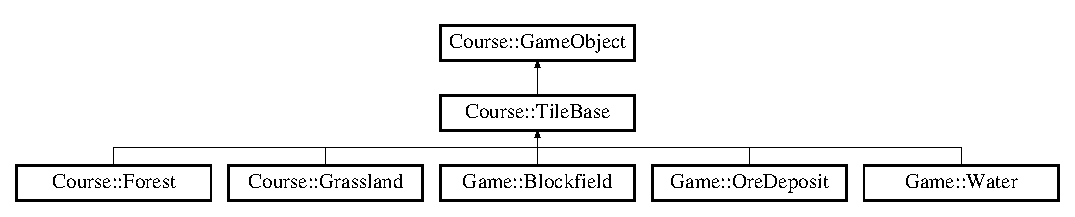
\includegraphics[height=2.470588cm]{classCourse_1_1TileBase}
\end{center}
\end{figure}
\subsection*{Public Member Functions}
\begin{DoxyCompactItemize}
\item 
\hyperlink{classCourse_1_1TileBase_a6386bf6bc05528b4337dee65f6286e06}{Tile\-Base} ()=delete
\begin{DoxyCompactList}\small\item\em Disabled parameterless constructor. \end{DoxyCompactList}\item 
\hyperlink{classCourse_1_1TileBase_ac1de1c7a0540691ef5a5c3321d12b708}{Tile\-Base} (const \hyperlink{classCourse_1_1Coordinate}{Coordinate} \&location, const std\-::shared\-\_\-ptr$<$ \hyperlink{classCourse_1_1iGameEventHandler}{i\-Game\-Event\-Handler} $>$ \&eventhandler, const std\-::shared\-\_\-ptr$<$ \hyperlink{classCourse_1_1iObjectManager}{i\-Object\-Manager} $>$ \&objectmanager, const unsigned int \&max\-\_\-build=2, const unsigned int \&max\-\_\-work=3, const \hyperlink{namespaceCourse_ab9a46ed9cd00485e318e5731ea2f78d9}{Resource\-Map} \&production=\{\})
\begin{DoxyCompactList}\small\item\em Constructor for the class. \end{DoxyCompactList}\item 
virtual \hyperlink{classCourse_1_1TileBase_a821db6b529d987eac53a958084fe2d5c}{$\sim$\-Tile\-Base} ()=default
\begin{DoxyCompactList}\small\item\em Default destructor. \end{DoxyCompactList}\item 
virtual std\-::string \hyperlink{classCourse_1_1TileBase_af1a8aaa3407ad3ade7ffe8f2fb421288}{get\-Type} () const override
\begin{DoxyCompactList}\small\item\em get\-Type Returns a string describing objects type. This should be overriden in each inherited class. Makes checking object's type easier for students. \end{DoxyCompactList}\item 
virtual void \hyperlink{classCourse_1_1TileBase_add69a1e9ec009dedb28ce54c8535370b}{add\-Building} (const std\-::shared\-\_\-ptr$<$ \hyperlink{classCourse_1_1BuildingBase}{Building\-Base} $>$ \&building)
\begin{DoxyCompactList}\small\item\em Adds a new Building-\/object to the tile. \end{DoxyCompactList}\item 
virtual void \hyperlink{classCourse_1_1TileBase_a0cb0e1f7b13ca68b452e6f4846266d87}{remove\-Building} (const std\-::shared\-\_\-ptr$<$ \hyperlink{classCourse_1_1BuildingBase}{Building\-Base} $>$ \&building)
\begin{DoxyCompactList}\small\item\em Removes a Building-\/object from this Tile. \end{DoxyCompactList}\item 
virtual void \hyperlink{classCourse_1_1TileBase_ac512085412a2f4b9b30841ed265fd706}{add\-Worker} (const std\-::shared\-\_\-ptr$<$ \hyperlink{classCourse_1_1WorkerBase}{Worker\-Base} $>$ \&worker)
\begin{DoxyCompactList}\small\item\em Adds a new Worker-\/object to this Tile. \end{DoxyCompactList}\item 
virtual void \hyperlink{classCourse_1_1TileBase_ad1a1a40e737037d29dc8ece6798439f6}{remove\-Worker} (const std\-::shared\-\_\-ptr$<$ \hyperlink{classCourse_1_1WorkerBase}{Worker\-Base} $>$ \&worker)
\begin{DoxyCompactList}\small\item\em Removes a Worker-\/object from this Tile. \end{DoxyCompactList}\item 
virtual bool \hyperlink{classCourse_1_1TileBase_a4cd675a5d9890fb63282bb2d72aa52af}{generate\-Resources} ()
\begin{DoxyCompactList}\small\item\em Sends information to the Event\-Handler on what resources were generated by this Tile. \par
. \end{DoxyCompactList}\item 
virtual unsigned int \hyperlink{classCourse_1_1TileBase_a1a2be339a96e122eedcd3d5d8dd7095d}{get\-Building\-Count} () const final
\begin{DoxyCompactList}\small\item\em Returns the amount of spaces that are being taken from the building-\/capacity. \end{DoxyCompactList}\item 
virtual unsigned int \hyperlink{classCourse_1_1TileBase_ae3a8601af95ed2e8b29f4c764c939f05}{get\-Worker\-Count} () const final
\begin{DoxyCompactList}\small\item\em Returns the amount of spaces that are being taken from the worker-\/capacity. \end{DoxyCompactList}\item 
virtual bool \hyperlink{classCourse_1_1TileBase_aae6c4d2e91f42fc16e5b622ae9c8b0de}{has\-Space\-For\-Workers} (int amount) const final
\begin{DoxyCompactList}\small\item\em Checks if the tile has enough space for workers. \end{DoxyCompactList}\item 
virtual bool \hyperlink{classCourse_1_1TileBase_aefed0bd9cf73d04e123d31e0e3935f6d}{has\-Space\-For\-Buildings} (int amount) const final
\begin{DoxyCompactList}\small\item\em Checks if the tile has enough space for buildings. \end{DoxyCompactList}\item 
virtual std\-::vector\\*
$<$ std\-::shared\-\_\-ptr$<$ \hyperlink{classCourse_1_1WorkerBase}{Worker\-Base} $>$ $>$ \hyperlink{classCourse_1_1TileBase_a1236e96c0a4e745f8f2e56933d09b52a}{get\-Workers} () const final
\begin{DoxyCompactList}\small\item\em Returns a vector of pointers to Workers in the Tile. \end{DoxyCompactList}\item 
virtual std\-::vector\\*
$<$ std\-::shared\-\_\-ptr\\*
$<$ \hyperlink{classCourse_1_1BuildingBase}{Building\-Base} $>$ $>$ \hyperlink{classCourse_1_1TileBase_a95790d2cf8c86b96a3bfaf4958becfd5}{get\-Buildings} () const final
\begin{DoxyCompactList}\small\item\em Returns a vector of pointer to Buildings in the Tile. \end{DoxyCompactList}\end{DoxyCompactItemize}
\subsection*{Public Attributes}
\begin{DoxyCompactItemize}
\item 
const unsigned int \hyperlink{classCourse_1_1TileBase_a1c968e242544a994bfd54f73cd9027ea}{M\-A\-X\-\_\-\-B\-U\-I\-L\-D\-I\-N\-G\-S}
\item 
const unsigned int \hyperlink{classCourse_1_1TileBase_aebadbc88dff462405047769cab680909}{M\-A\-X\-\_\-\-W\-O\-R\-K\-E\-R\-S}
\item 
const \hyperlink{namespaceCourse_ab9a46ed9cd00485e318e5731ea2f78d9}{Resource\-Map} \hyperlink{classCourse_1_1TileBase_a62cd84d3705c6cca9afd0cb992dd4f02}{B\-A\-S\-E\-\_\-\-P\-R\-O\-D\-U\-C\-T\-I\-O\-N}
\end{DoxyCompactItemize}
\subsection*{Private Attributes}
\begin{DoxyCompactItemize}
\item 
std\-::vector$<$ std\-::weak\-\_\-ptr\\*
$<$ \hyperlink{classCourse_1_1WorkerBase}{Worker\-Base} $>$ $>$ \hyperlink{classCourse_1_1TileBase_ad77f32b276a9c86637078dcea1e47a3d}{m\-\_\-workers}
\item 
std\-::vector$<$ std\-::weak\-\_\-ptr\\*
$<$ \hyperlink{classCourse_1_1BuildingBase}{Building\-Base} $>$ $>$ \hyperlink{classCourse_1_1TileBase_a69655ffca55e85254b87da39cf3b86b9}{m\-\_\-buildings}
\end{DoxyCompactItemize}
\subsection*{Additional Inherited Members}


\subsection{Detailed Description}
The \hyperlink{classCourse_1_1TileBase}{Tile\-Base} class is a base-\/class for different Tile-\/objects in the game. \par
. 

Tile is responsible for\-:
\begin{DoxyItemize}
\item Generating resources.
\item Checking Tile-\/specific object placement rules. \par
 Each Tile has some Base-\/production which is multiplied by worker's efficiency, when generating resources. Resource generation can also gain flat bonuses from buildings. Tiles also know how many Buildings or Workers can be placed on them. 
\end{DoxyItemize}

\subsection{Constructor \& Destructor Documentation}
\hypertarget{classCourse_1_1TileBase_a6386bf6bc05528b4337dee65f6286e06}{\index{Course\-::\-Tile\-Base@{Course\-::\-Tile\-Base}!Tile\-Base@{Tile\-Base}}
\index{Tile\-Base@{Tile\-Base}!Course::TileBase@{Course\-::\-Tile\-Base}}
\subsubsection[{Tile\-Base}]{\setlength{\rightskip}{0pt plus 5cm}Course\-::\-Tile\-Base\-::\-Tile\-Base (
\begin{DoxyParamCaption}
{}
\end{DoxyParamCaption}
)\hspace{0.3cm}{\ttfamily [delete]}}}\label{classCourse_1_1TileBase_a6386bf6bc05528b4337dee65f6286e06}


Disabled parameterless constructor. 

\hypertarget{classCourse_1_1TileBase_ac1de1c7a0540691ef5a5c3321d12b708}{\index{Course\-::\-Tile\-Base@{Course\-::\-Tile\-Base}!Tile\-Base@{Tile\-Base}}
\index{Tile\-Base@{Tile\-Base}!Course::TileBase@{Course\-::\-Tile\-Base}}
\subsubsection[{Tile\-Base}]{\setlength{\rightskip}{0pt plus 5cm}Course\-::\-Tile\-Base\-::\-Tile\-Base (
\begin{DoxyParamCaption}
\item[{const {\bf Coordinate} \&}]{location, }
\item[{const std\-::shared\-\_\-ptr$<$ {\bf i\-Game\-Event\-Handler} $>$ \&}]{eventhandler, }
\item[{const std\-::shared\-\_\-ptr$<$ {\bf i\-Object\-Manager} $>$ \&}]{objectmanager, }
\item[{const unsigned int \&}]{max\-\_\-build = {\ttfamily 2}, }
\item[{const unsigned int \&}]{max\-\_\-work = {\ttfamily 3}, }
\item[{const {\bf Resource\-Map} \&}]{production = {\ttfamily \{\}}}
\end{DoxyParamCaption}
)}}\label{classCourse_1_1TileBase_ac1de1c7a0540691ef5a5c3321d12b708}


Constructor for the class. 

\hypertarget{classCourse_1_1TileBase_a821db6b529d987eac53a958084fe2d5c}{\index{Course\-::\-Tile\-Base@{Course\-::\-Tile\-Base}!$\sim$\-Tile\-Base@{$\sim$\-Tile\-Base}}
\index{$\sim$\-Tile\-Base@{$\sim$\-Tile\-Base}!Course::TileBase@{Course\-::\-Tile\-Base}}
\subsubsection[{$\sim$\-Tile\-Base}]{\setlength{\rightskip}{0pt plus 5cm}virtual Course\-::\-Tile\-Base\-::$\sim$\-Tile\-Base (
\begin{DoxyParamCaption}
{}
\end{DoxyParamCaption}
)\hspace{0.3cm}{\ttfamily [virtual]}, {\ttfamily [default]}}}\label{classCourse_1_1TileBase_a821db6b529d987eac53a958084fe2d5c}


Default destructor. 



\subsection{Member Function Documentation}
\hypertarget{classCourse_1_1TileBase_add69a1e9ec009dedb28ce54c8535370b}{\index{Course\-::\-Tile\-Base@{Course\-::\-Tile\-Base}!add\-Building@{add\-Building}}
\index{add\-Building@{add\-Building}!Course::TileBase@{Course\-::\-Tile\-Base}}
\subsubsection[{add\-Building}]{\setlength{\rightskip}{0pt plus 5cm}void Course\-::\-Tile\-Base\-::add\-Building (
\begin{DoxyParamCaption}
\item[{const std\-::shared\-\_\-ptr$<$ {\bf Building\-Base} $>$ \&}]{building}
\end{DoxyParamCaption}
)\hspace{0.3cm}{\ttfamily [virtual]}}}\label{classCourse_1_1TileBase_add69a1e9ec009dedb28ce54c8535370b}


Adds a new Building-\/object to the tile. 

Phases\-: \par

\begin{DoxyEnumerate}
\item Tile checks if it has space for the building. \par

\item Building checks whether it can be placed on this tile. \par

\item Building is added to this Tile. \par

\item Tile update's Building's location. \par
 
\begin{DoxyParams}{Parameters}
{\em building} & A pointer to the Building that is being added. \\
\hline
\end{DoxyParams}
\begin{DoxyPostcond}{Postcondition}
Exception guarantee\-: Basic 
\end{DoxyPostcond}

\begin{DoxyExceptions}{Exceptions}
{\em \hyperlink{classCourse_1_1InvalidPointer}{Invalid\-Pointer}} & -\/ If the building's pointer doesn't point to anything or Object\-Manager doesn't return valid shared\-\_\-ptr to this tile. \\
\hline
{\em Illegal\-Move} & -\/ Any Illegal\-Exception can be thrown by a Tile or Building if it breaks a placement rule. \\
\hline
{\em \hyperlink{classCourse_1_1NotEnoughSpace}{Not\-Enough\-Space}} & (Illegal\-Move) -\/ If the tile doesn't have enough space for the Building. \\
\hline
\end{DoxyExceptions}

\end{DoxyEnumerate}

Reimplemented in \hyperlink{classGame_1_1OreDeposit_af8a88425e59e4fbb12eb90cc70b22ac7}{Game\-::\-Ore\-Deposit}, \hyperlink{classGame_1_1Blockfield_a7b6ecdadde2797965d6fbbe640d664bc}{Game\-::\-Blockfield}, and \hyperlink{classCourse_1_1Forest_a16ad633cd25afa705fbaefbc42efc2ae}{Course\-::\-Forest}.

\hypertarget{classCourse_1_1TileBase_ac512085412a2f4b9b30841ed265fd706}{\index{Course\-::\-Tile\-Base@{Course\-::\-Tile\-Base}!add\-Worker@{add\-Worker}}
\index{add\-Worker@{add\-Worker}!Course::TileBase@{Course\-::\-Tile\-Base}}
\subsubsection[{add\-Worker}]{\setlength{\rightskip}{0pt plus 5cm}void Course\-::\-Tile\-Base\-::add\-Worker (
\begin{DoxyParamCaption}
\item[{const std\-::shared\-\_\-ptr$<$ {\bf Worker\-Base} $>$ \&}]{worker}
\end{DoxyParamCaption}
)\hspace{0.3cm}{\ttfamily [virtual]}}}\label{classCourse_1_1TileBase_ac512085412a2f4b9b30841ed265fd706}


Adds a new Worker-\/object to this Tile. 

Phases\-: \par

\begin{DoxyEnumerate}
\item Tile checks if it has space for the Worker. \par

\item Worker checks whether it can be placed on this Tile. \par

\item Worker is added to this Tile. \par

\item Tile updates Worker's location. \par
 
\begin{DoxyParams}{Parameters}
{\em worker} & A pointer to the Worker-\/object that is being added. \\
\hline
\end{DoxyParams}
\begin{DoxyPostcond}{Postcondition}
Exception guarantee\-: Basic 
\end{DoxyPostcond}

\begin{DoxyExceptions}{Exceptions}
{\em \hyperlink{classCourse_1_1InvalidPointer}{Invalid\-Pointer}} & -\/ If the Worker's pointer doesn't point to anything or Object\-Manager doesn't return valid shared\-\_\-ptr to this tile. \\
\hline
{\em Illegal\-Move} & -\/ Any Illegal\-Exception can be thrown by a Tile or Worker if it breaks a placement rule. \\
\hline
{\em \hyperlink{classCourse_1_1NotEnoughSpace}{Not\-Enough\-Space}} & (Illegal\-Move) -\/ If the tile doesn't have enough space for the Worker. \\
\hline
\end{DoxyExceptions}

\end{DoxyEnumerate}\hypertarget{classCourse_1_1TileBase_a4cd675a5d9890fb63282bb2d72aa52af}{\index{Course\-::\-Tile\-Base@{Course\-::\-Tile\-Base}!generate\-Resources@{generate\-Resources}}
\index{generate\-Resources@{generate\-Resources}!Course::TileBase@{Course\-::\-Tile\-Base}}
\subsubsection[{generate\-Resources}]{\setlength{\rightskip}{0pt plus 5cm}bool Course\-::\-Tile\-Base\-::generate\-Resources (
\begin{DoxyParamCaption}
{}
\end{DoxyParamCaption}
)\hspace{0.3cm}{\ttfamily [virtual]}}}\label{classCourse_1_1TileBase_a4cd675a5d9890fb63282bb2d72aa52af}


Sends information to the Event\-Handler on what resources were generated by this Tile. \par
. 


\begin{DoxyEnumerate}
\item Call tile\-Work\-Action for each Worker. \par

\item Calculate Tile's production based on Base-\/production multiplied by Workers' efficiency. \par

\item Calls buildings' get\-Production() and adds the flat bonus. \par

\item Sends information to Game\-Event\-Handler. \par

\item Returns Game\-Event\-Handler's response. \par
 \begin{DoxyPostcond}{Postcondition}
Exception guarantee\-: Basic 
\end{DoxyPostcond}

\end{DoxyEnumerate}\hypertarget{classCourse_1_1TileBase_a1a2be339a96e122eedcd3d5d8dd7095d}{\index{Course\-::\-Tile\-Base@{Course\-::\-Tile\-Base}!get\-Building\-Count@{get\-Building\-Count}}
\index{get\-Building\-Count@{get\-Building\-Count}!Course::TileBase@{Course\-::\-Tile\-Base}}
\subsubsection[{get\-Building\-Count}]{\setlength{\rightskip}{0pt plus 5cm}unsigned int Course\-::\-Tile\-Base\-::get\-Building\-Count (
\begin{DoxyParamCaption}
{}
\end{DoxyParamCaption}
) const\hspace{0.3cm}{\ttfamily [final]}, {\ttfamily [virtual]}}}\label{classCourse_1_1TileBase_a1a2be339a96e122eedcd3d5d8dd7095d}


Returns the amount of spaces that are being taken from the building-\/capacity. 

\begin{DoxyReturn}{Returns}
The amount of space taken. 
\end{DoxyReturn}
\begin{DoxyPostcond}{Postcondition}
Exception guarantee\-: No-\/throw 
\end{DoxyPostcond}
\hypertarget{classCourse_1_1TileBase_a95790d2cf8c86b96a3bfaf4958becfd5}{\index{Course\-::\-Tile\-Base@{Course\-::\-Tile\-Base}!get\-Buildings@{get\-Buildings}}
\index{get\-Buildings@{get\-Buildings}!Course::TileBase@{Course\-::\-Tile\-Base}}
\subsubsection[{get\-Buildings}]{\setlength{\rightskip}{0pt plus 5cm}std\-::vector$<$ std\-::shared\-\_\-ptr$<$ {\bf Building\-Base} $>$ $>$ Course\-::\-Tile\-Base\-::get\-Buildings (
\begin{DoxyParamCaption}
{}
\end{DoxyParamCaption}
) const\hspace{0.3cm}{\ttfamily [final]}, {\ttfamily [virtual]}}}\label{classCourse_1_1TileBase_a95790d2cf8c86b96a3bfaf4958becfd5}


Returns a vector of pointer to Buildings in the Tile. 

\begin{DoxyPostcond}{Postcondition}
Exception Guarantee\-: No-\/throw 
\end{DoxyPostcond}
\hypertarget{classCourse_1_1TileBase_af1a8aaa3407ad3ade7ffe8f2fb421288}{\index{Course\-::\-Tile\-Base@{Course\-::\-Tile\-Base}!get\-Type@{get\-Type}}
\index{get\-Type@{get\-Type}!Course::TileBase@{Course\-::\-Tile\-Base}}
\subsubsection[{get\-Type}]{\setlength{\rightskip}{0pt plus 5cm}std\-::string Course\-::\-Tile\-Base\-::get\-Type (
\begin{DoxyParamCaption}
{}
\end{DoxyParamCaption}
) const\hspace{0.3cm}{\ttfamily [override]}, {\ttfamily [virtual]}}}\label{classCourse_1_1TileBase_af1a8aaa3407ad3ade7ffe8f2fb421288}


get\-Type Returns a string describing objects type. This should be overriden in each inherited class. Makes checking object's type easier for students. 

\begin{DoxyReturn}{Returns}
std\-::string that represents Object's type. 
\end{DoxyReturn}
\begin{DoxyPostcond}{Postcondition}
Exception guarantee\-: No-\/throw 
\end{DoxyPostcond}
\begin{DoxyNote}{Note}
You can use this in e.\-g. debugging and similar printing. 
\end{DoxyNote}


Reimplemented from \hyperlink{classCourse_1_1GameObject_aeecb0b8f5ed8d7b379e0e38ef4ebba10}{Course\-::\-Game\-Object}.



Reimplemented in \hyperlink{classGame_1_1OreDeposit_acc2ba331cb40a464821fe6ebaaf63573}{Game\-::\-Ore\-Deposit}, \hyperlink{classGame_1_1Blockfield_af5e2a4c262cb1f59e442b60c8404b715}{Game\-::\-Blockfield}, \hyperlink{classGame_1_1Water_ab45fa1bb08eb0893d7bec1a97e7b22f0}{Game\-::\-Water}, \hyperlink{classCourse_1_1Grassland_a0a652bbecdda0216613dad980936e30e}{Course\-::\-Grassland}, and \hyperlink{classCourse_1_1Forest_a783378b8f5c1ec5d0c5c4a771291a902}{Course\-::\-Forest}.

\hypertarget{classCourse_1_1TileBase_ae3a8601af95ed2e8b29f4c764c939f05}{\index{Course\-::\-Tile\-Base@{Course\-::\-Tile\-Base}!get\-Worker\-Count@{get\-Worker\-Count}}
\index{get\-Worker\-Count@{get\-Worker\-Count}!Course::TileBase@{Course\-::\-Tile\-Base}}
\subsubsection[{get\-Worker\-Count}]{\setlength{\rightskip}{0pt plus 5cm}unsigned int Course\-::\-Tile\-Base\-::get\-Worker\-Count (
\begin{DoxyParamCaption}
{}
\end{DoxyParamCaption}
) const\hspace{0.3cm}{\ttfamily [final]}, {\ttfamily [virtual]}}}\label{classCourse_1_1TileBase_ae3a8601af95ed2e8b29f4c764c939f05}


Returns the amount of spaces that are being taken from the worker-\/capacity. 

\begin{DoxyReturn}{Returns}
The amount of space taken. 
\end{DoxyReturn}
\begin{DoxyPostcond}{Postcondition}
Exception guarantee\-: No-\/throw 
\end{DoxyPostcond}
\hypertarget{classCourse_1_1TileBase_a1236e96c0a4e745f8f2e56933d09b52a}{\index{Course\-::\-Tile\-Base@{Course\-::\-Tile\-Base}!get\-Workers@{get\-Workers}}
\index{get\-Workers@{get\-Workers}!Course::TileBase@{Course\-::\-Tile\-Base}}
\subsubsection[{get\-Workers}]{\setlength{\rightskip}{0pt plus 5cm}std\-::vector$<$ std\-::shared\-\_\-ptr$<$ {\bf Worker\-Base} $>$ $>$ Course\-::\-Tile\-Base\-::get\-Workers (
\begin{DoxyParamCaption}
{}
\end{DoxyParamCaption}
) const\hspace{0.3cm}{\ttfamily [final]}, {\ttfamily [virtual]}}}\label{classCourse_1_1TileBase_a1236e96c0a4e745f8f2e56933d09b52a}


Returns a vector of pointers to Workers in the Tile. 

\begin{DoxyPostcond}{Postcondition}
Exception Guarantee\-: No-\/throw 
\end{DoxyPostcond}
\hypertarget{classCourse_1_1TileBase_aefed0bd9cf73d04e123d31e0e3935f6d}{\index{Course\-::\-Tile\-Base@{Course\-::\-Tile\-Base}!has\-Space\-For\-Buildings@{has\-Space\-For\-Buildings}}
\index{has\-Space\-For\-Buildings@{has\-Space\-For\-Buildings}!Course::TileBase@{Course\-::\-Tile\-Base}}
\subsubsection[{has\-Space\-For\-Buildings}]{\setlength{\rightskip}{0pt plus 5cm}bool Course\-::\-Tile\-Base\-::has\-Space\-For\-Buildings (
\begin{DoxyParamCaption}
\item[{int}]{amount}
\end{DoxyParamCaption}
) const\hspace{0.3cm}{\ttfamily [final]}, {\ttfamily [virtual]}}}\label{classCourse_1_1TileBase_aefed0bd9cf73d04e123d31e0e3935f6d}


Checks if the tile has enough space for buildings. 


\begin{DoxyParams}{Parameters}
{\em amount} & Amount of buildingspace wanted. \\
\hline
\end{DoxyParams}
\begin{DoxyNote}{Note}
Uses get\-Max\-Buildings() 
\end{DoxyNote}
\begin{DoxyPostcond}{Postcondition}
Exception guarantee\-: No-\/throw 
\end{DoxyPostcond}
\hypertarget{classCourse_1_1TileBase_aae6c4d2e91f42fc16e5b622ae9c8b0de}{\index{Course\-::\-Tile\-Base@{Course\-::\-Tile\-Base}!has\-Space\-For\-Workers@{has\-Space\-For\-Workers}}
\index{has\-Space\-For\-Workers@{has\-Space\-For\-Workers}!Course::TileBase@{Course\-::\-Tile\-Base}}
\subsubsection[{has\-Space\-For\-Workers}]{\setlength{\rightskip}{0pt plus 5cm}bool Course\-::\-Tile\-Base\-::has\-Space\-For\-Workers (
\begin{DoxyParamCaption}
\item[{int}]{amount}
\end{DoxyParamCaption}
) const\hspace{0.3cm}{\ttfamily [final]}, {\ttfamily [virtual]}}}\label{classCourse_1_1TileBase_aae6c4d2e91f42fc16e5b622ae9c8b0de}


Checks if the tile has enough space for workers. 


\begin{DoxyParams}{Parameters}
{\em amount} & Amount of workerspace wanted. \\
\hline
\end{DoxyParams}
\begin{DoxyNote}{Note}
Uses get\-Max\-Workers() 
\end{DoxyNote}
\begin{DoxyPostcond}{Postcondition}
Exception guarantee\-: No-\/throw 
\end{DoxyPostcond}
\hypertarget{classCourse_1_1TileBase_a0cb0e1f7b13ca68b452e6f4846266d87}{\index{Course\-::\-Tile\-Base@{Course\-::\-Tile\-Base}!remove\-Building@{remove\-Building}}
\index{remove\-Building@{remove\-Building}!Course::TileBase@{Course\-::\-Tile\-Base}}
\subsubsection[{remove\-Building}]{\setlength{\rightskip}{0pt plus 5cm}void Course\-::\-Tile\-Base\-::remove\-Building (
\begin{DoxyParamCaption}
\item[{const std\-::shared\-\_\-ptr$<$ {\bf Building\-Base} $>$ \&}]{building}
\end{DoxyParamCaption}
)\hspace{0.3cm}{\ttfamily [virtual]}}}\label{classCourse_1_1TileBase_a0cb0e1f7b13ca68b452e6f4846266d87}


Removes a Building-\/object from this Tile. 

Phases\-: \par

\begin{DoxyEnumerate}
\item Reset the Building's location to nothing. \par

\item Remove the Building from m\-\_\-buildings.
\end{DoxyEnumerate}


\begin{DoxyParams}{Parameters}
{\em building} & A pointer to the Building-\/object being removed. \\
\hline
\end{DoxyParams}
\begin{DoxyPostcond}{Postcondition}
Exception guarantee\-: Basic 
\end{DoxyPostcond}

\begin{DoxyExceptions}{Exceptions}
{\em \hyperlink{classCourse_1_1InvalidPointer}{Invalid\-Pointer}} & -\/ If the Building's pointer doesn't point to anything. \\
\hline
\end{DoxyExceptions}
\hypertarget{classCourse_1_1TileBase_ad1a1a40e737037d29dc8ece6798439f6}{\index{Course\-::\-Tile\-Base@{Course\-::\-Tile\-Base}!remove\-Worker@{remove\-Worker}}
\index{remove\-Worker@{remove\-Worker}!Course::TileBase@{Course\-::\-Tile\-Base}}
\subsubsection[{remove\-Worker}]{\setlength{\rightskip}{0pt plus 5cm}void Course\-::\-Tile\-Base\-::remove\-Worker (
\begin{DoxyParamCaption}
\item[{const std\-::shared\-\_\-ptr$<$ {\bf Worker\-Base} $>$ \&}]{worker}
\end{DoxyParamCaption}
)\hspace{0.3cm}{\ttfamily [virtual]}}}\label{classCourse_1_1TileBase_ad1a1a40e737037d29dc8ece6798439f6}


Removes a Worker-\/object from this Tile. 

Phases\-: \par

\begin{DoxyEnumerate}
\item Reset the Worker's location to nothing. \par

\item Remove the Worker from this Tile. \par
 
\begin{DoxyParams}{Parameters}
{\em worker} & A pointer to the Worker-\/object being removed. \\
\hline
\end{DoxyParams}

\begin{DoxyExceptions}{Exceptions}
{\em \hyperlink{classCourse_1_1InvalidPointer}{Invalid\-Pointer}} & -\/ If the Worker's pointer doesn't point to anything. \\
\hline
\end{DoxyExceptions}
\begin{DoxyPostcond}{Postcondition}
Exception guarantee\-: Basic  See std\-::vector\-::erase 
\end{DoxyPostcond}

\end{DoxyEnumerate}

\subsection{Member Data Documentation}
\hypertarget{classCourse_1_1TileBase_a62cd84d3705c6cca9afd0cb992dd4f02}{\index{Course\-::\-Tile\-Base@{Course\-::\-Tile\-Base}!B\-A\-S\-E\-\_\-\-P\-R\-O\-D\-U\-C\-T\-I\-O\-N@{B\-A\-S\-E\-\_\-\-P\-R\-O\-D\-U\-C\-T\-I\-O\-N}}
\index{B\-A\-S\-E\-\_\-\-P\-R\-O\-D\-U\-C\-T\-I\-O\-N@{B\-A\-S\-E\-\_\-\-P\-R\-O\-D\-U\-C\-T\-I\-O\-N}!Course::TileBase@{Course\-::\-Tile\-Base}}
\subsubsection[{B\-A\-S\-E\-\_\-\-P\-R\-O\-D\-U\-C\-T\-I\-O\-N}]{\setlength{\rightskip}{0pt plus 5cm}const {\bf Resource\-Map} Course\-::\-Tile\-Base\-::\-B\-A\-S\-E\-\_\-\-P\-R\-O\-D\-U\-C\-T\-I\-O\-N}}\label{classCourse_1_1TileBase_a62cd84d3705c6cca9afd0cb992dd4f02}
\hypertarget{classCourse_1_1TileBase_a69655ffca55e85254b87da39cf3b86b9}{\index{Course\-::\-Tile\-Base@{Course\-::\-Tile\-Base}!m\-\_\-buildings@{m\-\_\-buildings}}
\index{m\-\_\-buildings@{m\-\_\-buildings}!Course::TileBase@{Course\-::\-Tile\-Base}}
\subsubsection[{m\-\_\-buildings}]{\setlength{\rightskip}{0pt plus 5cm}std\-::vector$<$std\-::weak\-\_\-ptr$<${\bf Building\-Base}$>$ $>$ Course\-::\-Tile\-Base\-::m\-\_\-buildings\hspace{0.3cm}{\ttfamily [private]}}}\label{classCourse_1_1TileBase_a69655ffca55e85254b87da39cf3b86b9}
\hypertarget{classCourse_1_1TileBase_ad77f32b276a9c86637078dcea1e47a3d}{\index{Course\-::\-Tile\-Base@{Course\-::\-Tile\-Base}!m\-\_\-workers@{m\-\_\-workers}}
\index{m\-\_\-workers@{m\-\_\-workers}!Course::TileBase@{Course\-::\-Tile\-Base}}
\subsubsection[{m\-\_\-workers}]{\setlength{\rightskip}{0pt plus 5cm}std\-::vector$<$std\-::weak\-\_\-ptr$<${\bf Worker\-Base}$>$ $>$ Course\-::\-Tile\-Base\-::m\-\_\-workers\hspace{0.3cm}{\ttfamily [private]}}}\label{classCourse_1_1TileBase_ad77f32b276a9c86637078dcea1e47a3d}
\hypertarget{classCourse_1_1TileBase_a1c968e242544a994bfd54f73cd9027ea}{\index{Course\-::\-Tile\-Base@{Course\-::\-Tile\-Base}!M\-A\-X\-\_\-\-B\-U\-I\-L\-D\-I\-N\-G\-S@{M\-A\-X\-\_\-\-B\-U\-I\-L\-D\-I\-N\-G\-S}}
\index{M\-A\-X\-\_\-\-B\-U\-I\-L\-D\-I\-N\-G\-S@{M\-A\-X\-\_\-\-B\-U\-I\-L\-D\-I\-N\-G\-S}!Course::TileBase@{Course\-::\-Tile\-Base}}
\subsubsection[{M\-A\-X\-\_\-\-B\-U\-I\-L\-D\-I\-N\-G\-S}]{\setlength{\rightskip}{0pt plus 5cm}const unsigned int Course\-::\-Tile\-Base\-::\-M\-A\-X\-\_\-\-B\-U\-I\-L\-D\-I\-N\-G\-S}}\label{classCourse_1_1TileBase_a1c968e242544a994bfd54f73cd9027ea}
\hypertarget{classCourse_1_1TileBase_aebadbc88dff462405047769cab680909}{\index{Course\-::\-Tile\-Base@{Course\-::\-Tile\-Base}!M\-A\-X\-\_\-\-W\-O\-R\-K\-E\-R\-S@{M\-A\-X\-\_\-\-W\-O\-R\-K\-E\-R\-S}}
\index{M\-A\-X\-\_\-\-W\-O\-R\-K\-E\-R\-S@{M\-A\-X\-\_\-\-W\-O\-R\-K\-E\-R\-S}!Course::TileBase@{Course\-::\-Tile\-Base}}
\subsubsection[{M\-A\-X\-\_\-\-W\-O\-R\-K\-E\-R\-S}]{\setlength{\rightskip}{0pt plus 5cm}const unsigned int Course\-::\-Tile\-Base\-::\-M\-A\-X\-\_\-\-W\-O\-R\-K\-E\-R\-S}}\label{classCourse_1_1TileBase_aebadbc88dff462405047769cab680909}


The documentation for this class was generated from the following files\-:\begin{DoxyCompactItemize}
\item 
Course/\-Course\-Lib/tiles/\hyperlink{tilebase_8h}{tilebase.\-h}\item 
Course/\-Course\-Lib/tiles/\hyperlink{tilebase_8cpp}{tilebase.\-cpp}\end{DoxyCompactItemize}

\hypertarget{classGame_1_1Water}{\section{Game\-:\-:Water Class Reference}
\label{classGame_1_1Water}\index{Game\-::\-Water@{Game\-::\-Water}}
}


The \hyperlink{classGame_1_1Water}{Water} class represents water in the gameworld.  




{\ttfamily \#include $<$water.\-h$>$}

Inheritance diagram for Game\-:\-:Water\-:\begin{figure}[H]
\begin{center}
\leavevmode
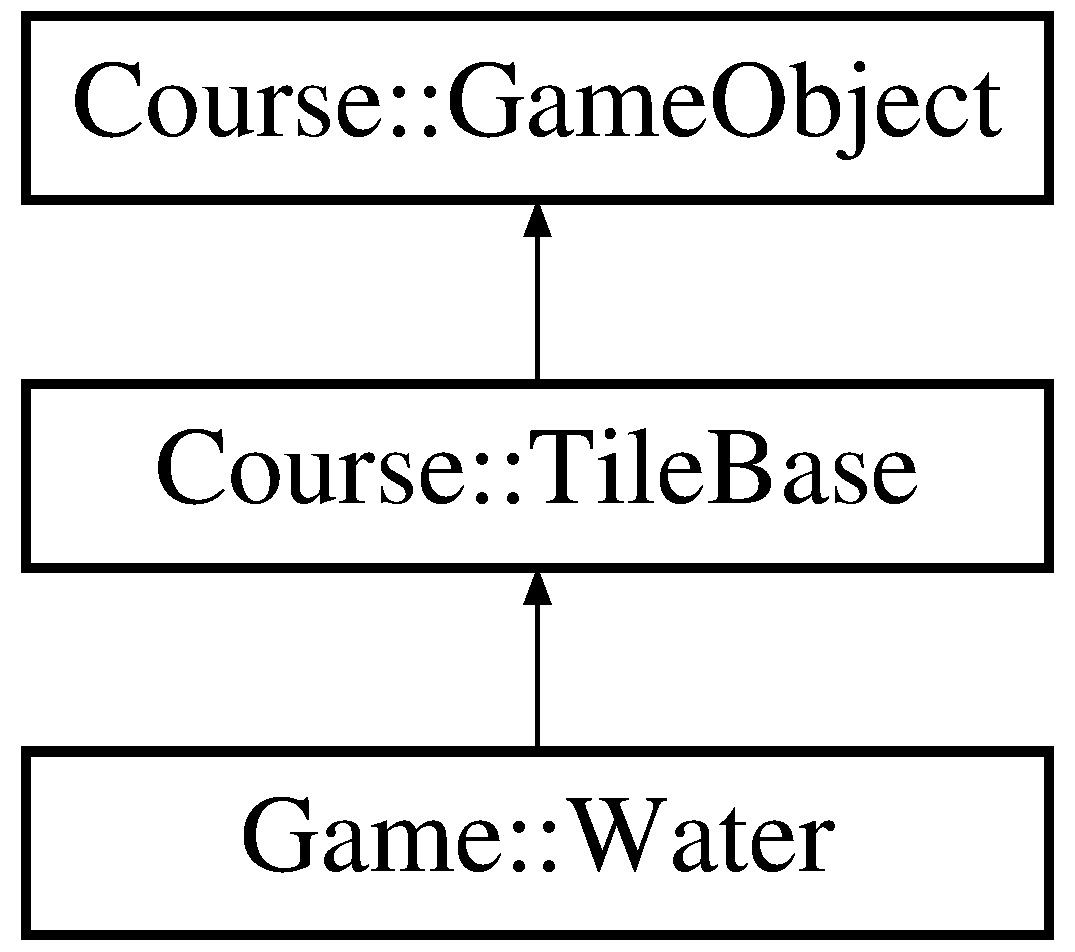
\includegraphics[height=3.000000cm]{classGame_1_1Water}
\end{center}
\end{figure}
\subsection*{Public Member Functions}
\begin{DoxyCompactItemize}
\item 
\hyperlink{classGame_1_1Water_a2f2918f6deef57b3e96ee63221002fee}{Water} ()=delete
\begin{DoxyCompactList}\small\item\em Disabled parameterless constructor. \end{DoxyCompactList}\item 
\hyperlink{classGame_1_1Water_a970774392539357ca258286489d9e679}{Water} (const \hyperlink{classCourse_1_1Coordinate}{Course\-::\-Coordinate} \&location, const std\-::shared\-\_\-ptr$<$ \hyperlink{classCourse_1_1iGameEventHandler}{Course\-::i\-Game\-Event\-Handler} $>$ \&eventhandler, const std\-::shared\-\_\-ptr$<$ \hyperlink{classCourse_1_1iObjectManager}{Course\-::i\-Object\-Manager} $>$ \&objectmanager, const unsigned int \&max\-\_\-build=0, const unsigned int \&max\-\_\-work=0, const \hyperlink{namespaceCourse_ab9a46ed9cd00485e318e5731ea2f78d9}{Course\-::\-Resource\-Map} \&production=\hyperlink{namespaceGame_1_1ConstResourceMaps_a0a964a6f0f80340d5a2d5a0a8dd0f79a}{Game\-::\-Const\-Resource\-Maps\-::\-W\-A\-T\-E\-R\-\_\-\-B\-P})
\begin{DoxyCompactList}\small\item\em Constructor for the class. \end{DoxyCompactList}\item 
virtual \hyperlink{classGame_1_1Water_ad714f7f3fd31960b7970e670070975f4}{$\sim$\-Water} ()=default
\begin{DoxyCompactList}\small\item\em Default destructor. \end{DoxyCompactList}\item 
virtual std\-::string \hyperlink{classGame_1_1Water_ab45fa1bb08eb0893d7bec1a97e7b22f0}{get\-Type} () const override
\end{DoxyCompactItemize}
\subsection*{Additional Inherited Members}


\subsection{Detailed Description}
The \hyperlink{classGame_1_1Water}{Water} class represents water in the gameworld. 

\hyperlink{classGame_1_1Water}{Water} has Basic\-Production\-: \par

\begin{DoxyItemize}
\item Money = 0
\item Food = 0
\item Wood = 0
\item Stone = 0
\item Ore = 0
\end{DoxyItemize}

You cannot build in water! 

\subsection{Constructor \& Destructor Documentation}
\hypertarget{classGame_1_1Water_a2f2918f6deef57b3e96ee63221002fee}{\index{Game\-::\-Water@{Game\-::\-Water}!Water@{Water}}
\index{Water@{Water}!Game::Water@{Game\-::\-Water}}
\subsubsection[{Water}]{\setlength{\rightskip}{0pt plus 5cm}Game\-::\-Water\-::\-Water (
\begin{DoxyParamCaption}
{}
\end{DoxyParamCaption}
)\hspace{0.3cm}{\ttfamily [delete]}}}\label{classGame_1_1Water_a2f2918f6deef57b3e96ee63221002fee}


Disabled parameterless constructor. 

\hypertarget{classGame_1_1Water_a970774392539357ca258286489d9e679}{\index{Game\-::\-Water@{Game\-::\-Water}!Water@{Water}}
\index{Water@{Water}!Game::Water@{Game\-::\-Water}}
\subsubsection[{Water}]{\setlength{\rightskip}{0pt plus 5cm}Game\-::\-Water\-::\-Water (
\begin{DoxyParamCaption}
\item[{const {\bf Course\-::\-Coordinate} \&}]{location, }
\item[{const std\-::shared\-\_\-ptr$<$ {\bf Course\-::i\-Game\-Event\-Handler} $>$ \&}]{eventhandler, }
\item[{const std\-::shared\-\_\-ptr$<$ {\bf Course\-::i\-Object\-Manager} $>$ \&}]{objectmanager, }
\item[{const unsigned int \&}]{max\-\_\-build = {\ttfamily 0}, }
\item[{const unsigned int \&}]{max\-\_\-work = {\ttfamily 0}, }
\item[{const {\bf Course\-::\-Resource\-Map} \&}]{production = {\ttfamily {\bf Game\-::\-Const\-Resource\-Maps\-::\-W\-A\-T\-E\-R\-\_\-\-B\-P}}}
\end{DoxyParamCaption}
)}}\label{classGame_1_1Water_a970774392539357ca258286489d9e679}


Constructor for the class. 


\begin{DoxyParams}{Parameters}
{\em location} & is the Coordinate where the Tile is located in the game. \\
\hline
{\em eventhandler} & points to the \hyperlink{classGame_1_1GameEventHandler}{Game\-Event\-Handler}. \\
\hline
{\em objectmanager} & points to the \hyperlink{classGame_1_1ObjectManager}{Object\-Manager}. \\
\hline
{\em max\-\_\-build} & defines maximum amount of buildings on the tile \\
\hline
{\em max\-\_\-work} & defines maximum amount of workers on the tile \\
\hline
{\em production} & sets the tiles production \\
\hline
\end{DoxyParams}
\hypertarget{classGame_1_1Water_ad714f7f3fd31960b7970e670070975f4}{\index{Game\-::\-Water@{Game\-::\-Water}!$\sim$\-Water@{$\sim$\-Water}}
\index{$\sim$\-Water@{$\sim$\-Water}!Game::Water@{Game\-::\-Water}}
\subsubsection[{$\sim$\-Water}]{\setlength{\rightskip}{0pt plus 5cm}virtual Game\-::\-Water\-::$\sim$\-Water (
\begin{DoxyParamCaption}
{}
\end{DoxyParamCaption}
)\hspace{0.3cm}{\ttfamily [virtual]}, {\ttfamily [default]}}}\label{classGame_1_1Water_ad714f7f3fd31960b7970e670070975f4}


Default destructor. 



\subsection{Member Function Documentation}
\hypertarget{classGame_1_1Water_ab45fa1bb08eb0893d7bec1a97e7b22f0}{\index{Game\-::\-Water@{Game\-::\-Water}!get\-Type@{get\-Type}}
\index{get\-Type@{get\-Type}!Game::Water@{Game\-::\-Water}}
\subsubsection[{get\-Type}]{\setlength{\rightskip}{0pt plus 5cm}std\-::string Game\-::\-Water\-::get\-Type (
\begin{DoxyParamCaption}
{}
\end{DoxyParamCaption}
) const\hspace{0.3cm}{\ttfamily [override]}, {\ttfamily [virtual]}}}\label{classGame_1_1Water_ab45fa1bb08eb0893d7bec1a97e7b22f0}






Reimplemented from \hyperlink{classCourse_1_1TileBase_af1a8aaa3407ad3ade7ffe8f2fb421288}{Course\-::\-Tile\-Base}.



The documentation for this class was generated from the following files\-:\begin{DoxyCompactItemize}
\item 
Game/tiles/\hyperlink{water_8h}{water.\-h}\item 
Game/tiles/\hyperlink{water_8cpp}{water.\-cpp}\end{DoxyCompactItemize}

\hypertarget{classCourse_1_1WorkerBase}{\section{Course\-:\-:Worker\-Base Class Reference}
\label{classCourse_1_1WorkerBase}\index{Course\-::\-Worker\-Base@{Course\-::\-Worker\-Base}}
}


The \hyperlink{classCourse_1_1WorkerBase}{Worker\-Base} class is an abstract base-\/class for Worker-\/objects.  




{\ttfamily \#include $<$workerbase.\-h$>$}

Inheritance diagram for Course\-:\-:Worker\-Base\-:\begin{figure}[H]
\begin{center}
\leavevmode
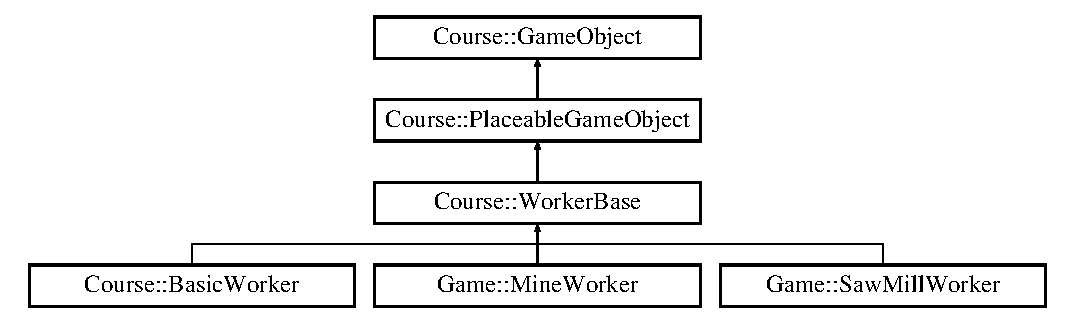
\includegraphics[height=3.888889cm]{classCourse_1_1WorkerBase}
\end{center}
\end{figure}
\subsection*{Public Member Functions}
\begin{DoxyCompactItemize}
\item 
\hyperlink{classCourse_1_1WorkerBase_a419f5f52654b70d123ea0c24bd94e091}{Worker\-Base} ()=delete
\begin{DoxyCompactList}\small\item\em Disabled parameterless constructor. \end{DoxyCompactList}\item 
\hyperlink{classCourse_1_1WorkerBase_af3dc160af36133a23d6e5bcd1ffe347e}{Worker\-Base} (const std\-::shared\-\_\-ptr$<$ \hyperlink{classCourse_1_1iGameEventHandler}{i\-Game\-Event\-Handler} $>$ \&eventhandler, const std\-::shared\-\_\-ptr$<$ \hyperlink{classCourse_1_1iObjectManager}{i\-Object\-Manager} $>$ \&objectmanager, const std\-::shared\-\_\-ptr$<$ \hyperlink{classCourse_1_1PlayerBase}{Player\-Base} $>$ \&owner, const int \&tilespaces=1, const \hyperlink{namespaceCourse_ab9a46ed9cd00485e318e5731ea2f78d9}{Resource\-Map} \&cost=\{\}, const \hyperlink{namespaceCourse_a0b96bae1a664dde34efbb1b42dea615e}{Resource\-Map\-Double} \&efficiency=\{\})
\item 
virtual \hyperlink{classCourse_1_1WorkerBase_a6711f994b4426907026fcc07ee77b429}{$\sim$\-Worker\-Base} ()=default
\begin{DoxyCompactList}\small\item\em Default destructor. \end{DoxyCompactList}\item 
virtual const \hyperlink{namespaceCourse_a0b96bae1a664dde34efbb1b42dea615e}{Resource\-Map\-Double} \hyperlink{classCourse_1_1WorkerBase_af0c1bb4f3bbea015e2a55aa6eff7f9ae}{tile\-Work\-Action} ()
\begin{DoxyCompactList}\small\item\em Performs worker's action when working a Tile for resources. \end{DoxyCompactList}\item 
virtual void \hyperlink{classCourse_1_1WorkerBase_a78553f35740e1c07d8f1071b5fc82212}{do\-Special\-Action} ()=0
\begin{DoxyCompactList}\small\item\em Performs the Worker's special action. (If any) \end{DoxyCompactList}\item 
virtual void \hyperlink{classCourse_1_1WorkerBase_a30335f9647eba9d04514be4bff059a6b}{set\-Resource\-Focus} (\hyperlink{namespaceCourse_a02d49c04029594d4adba79b84bb85f65}{Basic\-Resource} new\-\_\-focus) final
\begin{DoxyCompactList}\small\item\em Sets new resourcetype for the worker to focus on. \end{DoxyCompactList}\item 
virtual \hyperlink{namespaceCourse_a02d49c04029594d4adba79b84bb85f65}{Basic\-Resource} \hyperlink{classCourse_1_1WorkerBase_ac73fff2a6c99a353b80ea67425d5d545}{get\-Resource\-Focus} () const final
\begin{DoxyCompactList}\small\item\em Returns the currently focused resourcetype. \end{DoxyCompactList}\item 
virtual bool \hyperlink{classCourse_1_1WorkerBase_ad80874970ab91bca95b9d3f959e838d2}{can\-Be\-Placed\-On\-Tile} (const std\-::shared\-\_\-ptr$<$ \hyperlink{classCourse_1_1TileBase}{Tile\-Base} $>$ \&target) const override
\begin{DoxyCompactList}\small\item\em Default placement rule for workers\-:\par
. \end{DoxyCompactList}\item 
virtual std\-::string \hyperlink{classCourse_1_1WorkerBase_afe6049810eec47fffe2c2a7334564ef9}{get\-Type} () const override
\begin{DoxyCompactList}\small\item\em get\-Type Returns a string describing objects type. This should be overriden in each inherited class. Makes checking object's type easier for students. \end{DoxyCompactList}\end{DoxyCompactItemize}
\subsection*{Public Attributes}
\begin{DoxyCompactItemize}
\item 
const \hyperlink{namespaceCourse_a0b96bae1a664dde34efbb1b42dea615e}{Resource\-Map\-Double} \hyperlink{classCourse_1_1WorkerBase_ad20bcd4fba20ad9d287860cdaeedbcca}{W\-O\-R\-K\-E\-R\-\_\-\-E\-F\-F\-I\-C\-I\-E\-N\-C\-Y}
\item 
const \hyperlink{namespaceCourse_ab9a46ed9cd00485e318e5731ea2f78d9}{Resource\-Map} \hyperlink{classCourse_1_1WorkerBase_a0734e9b62296511492aca7c2ce531197}{R\-E\-C\-R\-U\-I\-T\-M\-E\-N\-T\-\_\-\-C\-O\-S\-T}
\end{DoxyCompactItemize}
\subsection*{Private Attributes}
\begin{DoxyCompactItemize}
\item 
\hyperlink{namespaceCourse_a02d49c04029594d4adba79b84bb85f65}{Basic\-Resource} \hyperlink{classCourse_1_1WorkerBase_aeb20af8ac5fede53f8bb68e41b87937c}{m\-\_\-resource\-\_\-focus}
\end{DoxyCompactItemize}
\subsection*{Additional Inherited Members}


\subsection{Detailed Description}
The \hyperlink{classCourse_1_1WorkerBase}{Worker\-Base} class is an abstract base-\/class for Worker-\/objects. 


\begin{DoxyItemize}
\item Workers can perform actions
\item Tiles request production-\/multipliers from Workers 
\end{DoxyItemize}

\subsection{Constructor \& Destructor Documentation}
\hypertarget{classCourse_1_1WorkerBase_a419f5f52654b70d123ea0c24bd94e091}{\index{Course\-::\-Worker\-Base@{Course\-::\-Worker\-Base}!Worker\-Base@{Worker\-Base}}
\index{Worker\-Base@{Worker\-Base}!Course::WorkerBase@{Course\-::\-Worker\-Base}}
\subsubsection[{Worker\-Base}]{\setlength{\rightskip}{0pt plus 5cm}Course\-::\-Worker\-Base\-::\-Worker\-Base (
\begin{DoxyParamCaption}
{}
\end{DoxyParamCaption}
)\hspace{0.3cm}{\ttfamily [delete]}}}\label{classCourse_1_1WorkerBase_a419f5f52654b70d123ea0c24bd94e091}


Disabled parameterless constructor. 

\hypertarget{classCourse_1_1WorkerBase_af3dc160af36133a23d6e5bcd1ffe347e}{\index{Course\-::\-Worker\-Base@{Course\-::\-Worker\-Base}!Worker\-Base@{Worker\-Base}}
\index{Worker\-Base@{Worker\-Base}!Course::WorkerBase@{Course\-::\-Worker\-Base}}
\subsubsection[{Worker\-Base}]{\setlength{\rightskip}{0pt plus 5cm}Course\-::\-Worker\-Base\-::\-Worker\-Base (
\begin{DoxyParamCaption}
\item[{const std\-::shared\-\_\-ptr$<$ {\bf i\-Game\-Event\-Handler} $>$ \&}]{eventhandler, }
\item[{const std\-::shared\-\_\-ptr$<$ {\bf i\-Object\-Manager} $>$ \&}]{objectmanager, }
\item[{const std\-::shared\-\_\-ptr$<$ {\bf Player\-Base} $>$ \&}]{owner, }
\item[{const int \&}]{tilespaces = {\ttfamily 1}, }
\item[{const {\bf Resource\-Map} \&}]{cost = {\ttfamily \{\}}, }
\item[{const {\bf Resource\-Map\-Double} \&}]{efficiency = {\ttfamily \{\}}}
\end{DoxyParamCaption}
)}}\label{classCourse_1_1WorkerBase_af3dc160af36133a23d6e5bcd1ffe347e}
\hypertarget{classCourse_1_1WorkerBase_a6711f994b4426907026fcc07ee77b429}{\index{Course\-::\-Worker\-Base@{Course\-::\-Worker\-Base}!$\sim$\-Worker\-Base@{$\sim$\-Worker\-Base}}
\index{$\sim$\-Worker\-Base@{$\sim$\-Worker\-Base}!Course::WorkerBase@{Course\-::\-Worker\-Base}}
\subsubsection[{$\sim$\-Worker\-Base}]{\setlength{\rightskip}{0pt plus 5cm}virtual Course\-::\-Worker\-Base\-::$\sim$\-Worker\-Base (
\begin{DoxyParamCaption}
{}
\end{DoxyParamCaption}
)\hspace{0.3cm}{\ttfamily [virtual]}, {\ttfamily [default]}}}\label{classCourse_1_1WorkerBase_a6711f994b4426907026fcc07ee77b429}


Default destructor. 



\subsection{Member Function Documentation}
\hypertarget{classCourse_1_1WorkerBase_ad80874970ab91bca95b9d3f959e838d2}{\index{Course\-::\-Worker\-Base@{Course\-::\-Worker\-Base}!can\-Be\-Placed\-On\-Tile@{can\-Be\-Placed\-On\-Tile}}
\index{can\-Be\-Placed\-On\-Tile@{can\-Be\-Placed\-On\-Tile}!Course::WorkerBase@{Course\-::\-Worker\-Base}}
\subsubsection[{can\-Be\-Placed\-On\-Tile}]{\setlength{\rightskip}{0pt plus 5cm}bool Course\-::\-Worker\-Base\-::can\-Be\-Placed\-On\-Tile (
\begin{DoxyParamCaption}
\item[{const std\-::shared\-\_\-ptr$<$ {\bf Tile\-Base} $>$ \&}]{target}
\end{DoxyParamCaption}
) const\hspace{0.3cm}{\ttfamily [override]}, {\ttfamily [virtual]}}}\label{classCourse_1_1WorkerBase_ad80874970ab91bca95b9d3f959e838d2}


Default placement rule for workers\-:\par
. 


\begin{DoxyItemize}
\item Tile must have space for the worker
\item Tile must have same owner as the worker 
\begin{DoxyParams}{Parameters}
{\em target} & is the Tile that worker is being placed on. \\
\hline
\end{DoxyParams}
\begin{DoxyReturn}{Returns}
True -\/ Only if both conditions are met. 
\end{DoxyReturn}
\begin{DoxyPostcond}{Postcondition}
Exception guarantee\-: Basic 
\end{DoxyPostcond}
\begin{DoxyNote}{Note}
Override to change placement rules for derived worker. 
\end{DoxyNote}

\end{DoxyItemize}

Reimplemented from \hyperlink{classCourse_1_1PlaceableGameObject_a09616c1b271c35df61c88b37d0b85968}{Course\-::\-Placeable\-Game\-Object}.



Reimplemented in \hyperlink{classGame_1_1MineWorker_aa52833ec99f6746871a78467c51bc57e}{Game\-::\-Mine\-Worker}, \hyperlink{classGame_1_1SawMillWorker_a435e13b35d129a453d7fdfcd60b6dc42}{Game\-::\-Saw\-Mill\-Worker}, and \hyperlink{classCourse_1_1BasicWorker_ab12d85004e92d9a1e85396d72c6cac98}{Course\-::\-Basic\-Worker}.

\hypertarget{classCourse_1_1WorkerBase_a78553f35740e1c07d8f1071b5fc82212}{\index{Course\-::\-Worker\-Base@{Course\-::\-Worker\-Base}!do\-Special\-Action@{do\-Special\-Action}}
\index{do\-Special\-Action@{do\-Special\-Action}!Course::WorkerBase@{Course\-::\-Worker\-Base}}
\subsubsection[{do\-Special\-Action}]{\setlength{\rightskip}{0pt plus 5cm}virtual void Course\-::\-Worker\-Base\-::do\-Special\-Action (
\begin{DoxyParamCaption}
{}
\end{DoxyParamCaption}
)\hspace{0.3cm}{\ttfamily [pure virtual]}}}\label{classCourse_1_1WorkerBase_a78553f35740e1c07d8f1071b5fc82212}


Performs the Worker's special action. (If any) 

\begin{DoxyNote}{Note}
Hint\-: You can use game-\/eventhandler for more creative solutions. 
\end{DoxyNote}


Implemented in \hyperlink{classGame_1_1MineWorker_a5faef20674a0d6408115461032e32edf}{Game\-::\-Mine\-Worker}, \hyperlink{classGame_1_1SawMillWorker_af344bff415417cb0c2744b038872221a}{Game\-::\-Saw\-Mill\-Worker}, and \hyperlink{classCourse_1_1BasicWorker_a626bab94f45602a34631c7ab6e60d829}{Course\-::\-Basic\-Worker}.

\hypertarget{classCourse_1_1WorkerBase_ac73fff2a6c99a353b80ea67425d5d545}{\index{Course\-::\-Worker\-Base@{Course\-::\-Worker\-Base}!get\-Resource\-Focus@{get\-Resource\-Focus}}
\index{get\-Resource\-Focus@{get\-Resource\-Focus}!Course::WorkerBase@{Course\-::\-Worker\-Base}}
\subsubsection[{get\-Resource\-Focus}]{\setlength{\rightskip}{0pt plus 5cm}{\bf Basic\-Resource} Course\-::\-Worker\-Base\-::get\-Resource\-Focus (
\begin{DoxyParamCaption}
{}
\end{DoxyParamCaption}
) const\hspace{0.3cm}{\ttfamily [final]}, {\ttfamily [virtual]}}}\label{classCourse_1_1WorkerBase_ac73fff2a6c99a353b80ea67425d5d545}


Returns the currently focused resourcetype. 

\begin{DoxyPostcond}{Postcondition}
Exception guarantee\-: No-\/throw 
\end{DoxyPostcond}
\hypertarget{classCourse_1_1WorkerBase_afe6049810eec47fffe2c2a7334564ef9}{\index{Course\-::\-Worker\-Base@{Course\-::\-Worker\-Base}!get\-Type@{get\-Type}}
\index{get\-Type@{get\-Type}!Course::WorkerBase@{Course\-::\-Worker\-Base}}
\subsubsection[{get\-Type}]{\setlength{\rightskip}{0pt plus 5cm}std\-::string Course\-::\-Worker\-Base\-::get\-Type (
\begin{DoxyParamCaption}
{}
\end{DoxyParamCaption}
) const\hspace{0.3cm}{\ttfamily [override]}, {\ttfamily [virtual]}}}\label{classCourse_1_1WorkerBase_afe6049810eec47fffe2c2a7334564ef9}


get\-Type Returns a string describing objects type. This should be overriden in each inherited class. Makes checking object's type easier for students. 

\begin{DoxyReturn}{Returns}
std\-::string that represents Object's type. 
\end{DoxyReturn}
\begin{DoxyPostcond}{Postcondition}
Exception guarantee\-: No-\/throw 
\end{DoxyPostcond}
\begin{DoxyNote}{Note}
You can use this in e.\-g. debugging and similar printing. 
\end{DoxyNote}


Reimplemented from \hyperlink{classCourse_1_1PlaceableGameObject_adcd0c91b52ccedd434092380644f210e}{Course\-::\-Placeable\-Game\-Object}.



Reimplemented in \hyperlink{classGame_1_1MineWorker_a984c2ede11ac50460620a4d982249dbe}{Game\-::\-Mine\-Worker}, \hyperlink{classGame_1_1SawMillWorker_af64ec6de521d31ec3fdc885a3bc69cba}{Game\-::\-Saw\-Mill\-Worker}, and \hyperlink{classCourse_1_1BasicWorker_a8396e00dafd128cbb86e479296d75c12}{Course\-::\-Basic\-Worker}.

\hypertarget{classCourse_1_1WorkerBase_a30335f9647eba9d04514be4bff059a6b}{\index{Course\-::\-Worker\-Base@{Course\-::\-Worker\-Base}!set\-Resource\-Focus@{set\-Resource\-Focus}}
\index{set\-Resource\-Focus@{set\-Resource\-Focus}!Course::WorkerBase@{Course\-::\-Worker\-Base}}
\subsubsection[{set\-Resource\-Focus}]{\setlength{\rightskip}{0pt plus 5cm}void Course\-::\-Worker\-Base\-::set\-Resource\-Focus (
\begin{DoxyParamCaption}
\item[{{\bf Basic\-Resource}}]{new\-\_\-focus}
\end{DoxyParamCaption}
)\hspace{0.3cm}{\ttfamily [final]}, {\ttfamily [virtual]}}}\label{classCourse_1_1WorkerBase_a30335f9647eba9d04514be4bff059a6b}


Sets new resourcetype for the worker to focus on. 


\begin{DoxyParams}{Parameters}
{\em new\-\_\-focus} & the new resource focus. \\
\hline
\end{DoxyParams}
\begin{DoxyPostcond}{Postcondition}
Exception guarantee\-: No-\/throw 
\end{DoxyPostcond}
\hypertarget{classCourse_1_1WorkerBase_af0c1bb4f3bbea015e2a55aa6eff7f9ae}{\index{Course\-::\-Worker\-Base@{Course\-::\-Worker\-Base}!tile\-Work\-Action@{tile\-Work\-Action}}
\index{tile\-Work\-Action@{tile\-Work\-Action}!Course::WorkerBase@{Course\-::\-Worker\-Base}}
\subsubsection[{tile\-Work\-Action}]{\setlength{\rightskip}{0pt plus 5cm}const {\bf Resource\-Map\-Double} Course\-::\-Worker\-Base\-::tile\-Work\-Action (
\begin{DoxyParamCaption}
{}
\end{DoxyParamCaption}
)\hspace{0.3cm}{\ttfamily [virtual]}}}\label{classCourse_1_1WorkerBase_af0c1bb4f3bbea015e2a55aa6eff7f9ae}


Performs worker's action when working a Tile for resources. 

\begin{DoxyReturn}{Returns}
Returns the final working efficiency of a worker. 
\end{DoxyReturn}
\begin{DoxyNote}{Note}
This is called by a Tile when it generates resources. 
\end{DoxyNote}


Reimplemented in \hyperlink{classGame_1_1MineWorker_a515a32b59f08ee1577210887166dacb0}{Game\-::\-Mine\-Worker}, \hyperlink{classGame_1_1SawMillWorker_a51596a8864954a22c6b69303b5e408d8}{Game\-::\-Saw\-Mill\-Worker}, and \hyperlink{classCourse_1_1BasicWorker_a870cf500ea86d30db583ce64299d9df4}{Course\-::\-Basic\-Worker}.



\subsection{Member Data Documentation}
\hypertarget{classCourse_1_1WorkerBase_aeb20af8ac5fede53f8bb68e41b87937c}{\index{Course\-::\-Worker\-Base@{Course\-::\-Worker\-Base}!m\-\_\-resource\-\_\-focus@{m\-\_\-resource\-\_\-focus}}
\index{m\-\_\-resource\-\_\-focus@{m\-\_\-resource\-\_\-focus}!Course::WorkerBase@{Course\-::\-Worker\-Base}}
\subsubsection[{m\-\_\-resource\-\_\-focus}]{\setlength{\rightskip}{0pt plus 5cm}{\bf Basic\-Resource} Course\-::\-Worker\-Base\-::m\-\_\-resource\-\_\-focus\hspace{0.3cm}{\ttfamily [private]}}}\label{classCourse_1_1WorkerBase_aeb20af8ac5fede53f8bb68e41b87937c}
\hypertarget{classCourse_1_1WorkerBase_a0734e9b62296511492aca7c2ce531197}{\index{Course\-::\-Worker\-Base@{Course\-::\-Worker\-Base}!R\-E\-C\-R\-U\-I\-T\-M\-E\-N\-T\-\_\-\-C\-O\-S\-T@{R\-E\-C\-R\-U\-I\-T\-M\-E\-N\-T\-\_\-\-C\-O\-S\-T}}
\index{R\-E\-C\-R\-U\-I\-T\-M\-E\-N\-T\-\_\-\-C\-O\-S\-T@{R\-E\-C\-R\-U\-I\-T\-M\-E\-N\-T\-\_\-\-C\-O\-S\-T}!Course::WorkerBase@{Course\-::\-Worker\-Base}}
\subsubsection[{R\-E\-C\-R\-U\-I\-T\-M\-E\-N\-T\-\_\-\-C\-O\-S\-T}]{\setlength{\rightskip}{0pt plus 5cm}const {\bf Resource\-Map} Course\-::\-Worker\-Base\-::\-R\-E\-C\-R\-U\-I\-T\-M\-E\-N\-T\-\_\-\-C\-O\-S\-T}}\label{classCourse_1_1WorkerBase_a0734e9b62296511492aca7c2ce531197}
\hypertarget{classCourse_1_1WorkerBase_ad20bcd4fba20ad9d287860cdaeedbcca}{\index{Course\-::\-Worker\-Base@{Course\-::\-Worker\-Base}!W\-O\-R\-K\-E\-R\-\_\-\-E\-F\-F\-I\-C\-I\-E\-N\-C\-Y@{W\-O\-R\-K\-E\-R\-\_\-\-E\-F\-F\-I\-C\-I\-E\-N\-C\-Y}}
\index{W\-O\-R\-K\-E\-R\-\_\-\-E\-F\-F\-I\-C\-I\-E\-N\-C\-Y@{W\-O\-R\-K\-E\-R\-\_\-\-E\-F\-F\-I\-C\-I\-E\-N\-C\-Y}!Course::WorkerBase@{Course\-::\-Worker\-Base}}
\subsubsection[{W\-O\-R\-K\-E\-R\-\_\-\-E\-F\-F\-I\-C\-I\-E\-N\-C\-Y}]{\setlength{\rightskip}{0pt plus 5cm}const {\bf Resource\-Map\-Double} Course\-::\-Worker\-Base\-::\-W\-O\-R\-K\-E\-R\-\_\-\-E\-F\-F\-I\-C\-I\-E\-N\-C\-Y}}\label{classCourse_1_1WorkerBase_ad20bcd4fba20ad9d287860cdaeedbcca}


The documentation for this class was generated from the following files\-:\begin{DoxyCompactItemize}
\item 
Course/\-Course\-Lib/workers/\hyperlink{workerbase_8h}{workerbase.\-h}\item 
Course/\-Course\-Lib/workers/\hyperlink{workerbase_8cpp}{workerbase.\-cpp}\end{DoxyCompactItemize}

\hypertarget{classCourse_1_1WorldGenerator}{\section{Course\-:\-:World\-Generator Class Reference}
\label{classCourse_1_1WorldGenerator}\index{Course\-::\-World\-Generator@{Course\-::\-World\-Generator}}
}


The \hyperlink{classCourse_1_1WorldGenerator}{World\-Generator} class is a singleton for generating tiles for the game.  




{\ttfamily \#include $<$worldgenerator.\-h$>$}

\subsection*{Public Member Functions}
\begin{DoxyCompactItemize}
\item 
\hyperlink{classCourse_1_1WorldGenerator_a4946730e80bc6cdc42761dec637f29b0}{World\-Generator} (const \hyperlink{classCourse_1_1WorldGenerator}{World\-Generator} \&)=delete
\item 
\hyperlink{classCourse_1_1WorldGenerator}{World\-Generator} \& \hyperlink{classCourse_1_1WorldGenerator_a9b75e71fa1d3522c78407c61c85defc3}{operator=} (const \hyperlink{classCourse_1_1WorldGenerator}{World\-Generator} \&)=delete
\item 
\hyperlink{classCourse_1_1WorldGenerator_a5e023cb70d8c3a76ad32add672d9d211}{World\-Generator} (\hyperlink{classCourse_1_1WorldGenerator}{World\-Generator} \&\&)=delete
\item 
\hyperlink{classCourse_1_1WorldGenerator}{World\-Generator} \& \hyperlink{classCourse_1_1WorldGenerator_ae1ad94ce5da50aeaf3365c86804c10ca}{operator=} (\hyperlink{classCourse_1_1WorldGenerator}{World\-Generator} \&\&)=delete
\item 
{\footnotesize template$<$typename T $>$ }\\void \hyperlink{classCourse_1_1WorldGenerator_adc7ea4ba3cba155910cdb03130c84e75}{add\-Constructor} (unsigned int weight)
\begin{DoxyCompactList}\small\item\em Register a Tile's constructor for use in map generation. \end{DoxyCompactList}\item 
void \hyperlink{classCourse_1_1WorldGenerator_a7fe4468658c14aac5bc282fda98245e1}{generate\-Map} (unsigned int size\-\_\-x, unsigned int size\-\_\-y, unsigned int seed, const std\-::shared\-\_\-ptr$<$ \hyperlink{classCourse_1_1iObjectManager}{i\-Object\-Manager} $>$ \&objectmanager, const std\-::shared\-\_\-ptr$<$ \hyperlink{classCourse_1_1iGameEventHandler}{i\-Game\-Event\-Handler} $>$ \&eventhandler)
\begin{DoxyCompactList}\small\item\em Generates Tile-\/objects and sends them to Object\-Manager. \end{DoxyCompactList}\end{DoxyCompactItemize}
\subsection*{Static Public Member Functions}
\begin{DoxyCompactItemize}
\item 
static \hyperlink{classCourse_1_1WorldGenerator}{World\-Generator} \& \hyperlink{classCourse_1_1WorldGenerator_a2b94f9ec5aa516b6528d90fa81868900}{get\-Instance} ()
\begin{DoxyCompactList}\small\item\em Used to get a reference to the Singleton instance. \end{DoxyCompactList}\end{DoxyCompactItemize}
\subsection*{Private Member Functions}
\begin{DoxyCompactItemize}
\item 
\hyperlink{classCourse_1_1WorldGenerator_a5f75bf6c9132d395a4ab0e5e68d1c599}{World\-Generator} ()=default
\begin{DoxyCompactList}\small\item\em Default constructor. \end{DoxyCompactList}\item 
\hyperlink{classCourse_1_1WorldGenerator_ae1cdc6937568b2a48b82040f4729e7a9}{$\sim$\-World\-Generator} ()=default
\begin{DoxyCompactList}\small\item\em Default destructor. \end{DoxyCompactList}\item 
\hyperlink{namespaceCourse_acf802ffd79a9573eb8afca22ae1f8a2f}{Tile\-Constructor\-Pointer} \hyperlink{classCourse_1_1WorldGenerator_a252f641fc41a3d89b86095f279d7a5fe}{find\-Rand\-Ctor} (int random) const 
\begin{DoxyCompactList}\small\item\em Find the Tile ctor matching the random number. \end{DoxyCompactList}\end{DoxyCompactItemize}
\subsection*{Private Attributes}
\begin{DoxyCompactItemize}
\item 
std\-::multimap$<$ unsigned int, \\*
\hyperlink{namespaceCourse_acf802ffd79a9573eb8afca22ae1f8a2f}{Tile\-Constructor\-Pointer} $>$ \hyperlink{classCourse_1_1WorldGenerator_aa4b7964b0d107de1248bb1cf0abb306a}{m\-\_\-ctors}
\end{DoxyCompactItemize}


\subsection{Detailed Description}
The \hyperlink{classCourse_1_1WorldGenerator}{World\-Generator} class is a singleton for generating tiles for the game. 

Students use this to create new Tile-\/objects that form the gameworld. \par
Usage\-:
\begin{DoxyEnumerate}
\item Use \hyperlink{classCourse_1_1WorldGenerator_a2b94f9ec5aa516b6528d90fa81868900}{World\-Generator\-::get\-Instance()} to get a reference to the singleton.
\item Call add\-Constructor with each Tile type you created.
\item Generate the map through the reference. 
\end{DoxyEnumerate}

\subsection{Constructor \& Destructor Documentation}
\hypertarget{classCourse_1_1WorldGenerator_a4946730e80bc6cdc42761dec637f29b0}{\index{Course\-::\-World\-Generator@{Course\-::\-World\-Generator}!World\-Generator@{World\-Generator}}
\index{World\-Generator@{World\-Generator}!Course::WorldGenerator@{Course\-::\-World\-Generator}}
\subsubsection[{World\-Generator}]{\setlength{\rightskip}{0pt plus 5cm}Course\-::\-World\-Generator\-::\-World\-Generator (
\begin{DoxyParamCaption}
\item[{const {\bf World\-Generator} \&}]{}
\end{DoxyParamCaption}
)\hspace{0.3cm}{\ttfamily [delete]}}}\label{classCourse_1_1WorldGenerator_a4946730e80bc6cdc42761dec637f29b0}
\hypertarget{classCourse_1_1WorldGenerator_a5e023cb70d8c3a76ad32add672d9d211}{\index{Course\-::\-World\-Generator@{Course\-::\-World\-Generator}!World\-Generator@{World\-Generator}}
\index{World\-Generator@{World\-Generator}!Course::WorldGenerator@{Course\-::\-World\-Generator}}
\subsubsection[{World\-Generator}]{\setlength{\rightskip}{0pt plus 5cm}Course\-::\-World\-Generator\-::\-World\-Generator (
\begin{DoxyParamCaption}
\item[{{\bf World\-Generator} \&\&}]{}
\end{DoxyParamCaption}
)\hspace{0.3cm}{\ttfamily [delete]}}}\label{classCourse_1_1WorldGenerator_a5e023cb70d8c3a76ad32add672d9d211}
\hypertarget{classCourse_1_1WorldGenerator_a5f75bf6c9132d395a4ab0e5e68d1c599}{\index{Course\-::\-World\-Generator@{Course\-::\-World\-Generator}!World\-Generator@{World\-Generator}}
\index{World\-Generator@{World\-Generator}!Course::WorldGenerator@{Course\-::\-World\-Generator}}
\subsubsection[{World\-Generator}]{\setlength{\rightskip}{0pt plus 5cm}Course\-::\-World\-Generator\-::\-World\-Generator (
\begin{DoxyParamCaption}
{}
\end{DoxyParamCaption}
)\hspace{0.3cm}{\ttfamily [private]}, {\ttfamily [default]}}}\label{classCourse_1_1WorldGenerator_a5f75bf6c9132d395a4ab0e5e68d1c599}


Default constructor. 

\hypertarget{classCourse_1_1WorldGenerator_ae1cdc6937568b2a48b82040f4729e7a9}{\index{Course\-::\-World\-Generator@{Course\-::\-World\-Generator}!$\sim$\-World\-Generator@{$\sim$\-World\-Generator}}
\index{$\sim$\-World\-Generator@{$\sim$\-World\-Generator}!Course::WorldGenerator@{Course\-::\-World\-Generator}}
\subsubsection[{$\sim$\-World\-Generator}]{\setlength{\rightskip}{0pt plus 5cm}Course\-::\-World\-Generator\-::$\sim$\-World\-Generator (
\begin{DoxyParamCaption}
{}
\end{DoxyParamCaption}
)\hspace{0.3cm}{\ttfamily [private]}, {\ttfamily [default]}}}\label{classCourse_1_1WorldGenerator_ae1cdc6937568b2a48b82040f4729e7a9}


Default destructor. 



\subsection{Member Function Documentation}
\hypertarget{classCourse_1_1WorldGenerator_adc7ea4ba3cba155910cdb03130c84e75}{\index{Course\-::\-World\-Generator@{Course\-::\-World\-Generator}!add\-Constructor@{add\-Constructor}}
\index{add\-Constructor@{add\-Constructor}!Course::WorldGenerator@{Course\-::\-World\-Generator}}
\subsubsection[{add\-Constructor}]{\setlength{\rightskip}{0pt plus 5cm}template$<$typename T $>$ void Course\-::\-World\-Generator\-::add\-Constructor (
\begin{DoxyParamCaption}
\item[{unsigned int}]{weight}
\end{DoxyParamCaption}
)\hspace{0.3cm}{\ttfamily [inline]}}}\label{classCourse_1_1WorldGenerator_adc7ea4ba3cba155910cdb03130c84e75}


Register a Tile's constructor for use in map generation. 

\begin{DoxyNote}{Note}
Do this only once per Tile type or they won't be equally common. Use the Tile's type as the template parameter\-: \hyperlink{classCourse_1_1WorldGenerator_adc7ea4ba3cba155910cdb03130c84e75}{add\-Constructor$<$\-Forest$>$()}; 
\end{DoxyNote}

\begin{DoxyParams}{Parameters}
{\em weight} & represents the rarity of the Tile, high being common. \\
\hline
\end{DoxyParams}
\hypertarget{classCourse_1_1WorldGenerator_a252f641fc41a3d89b86095f279d7a5fe}{\index{Course\-::\-World\-Generator@{Course\-::\-World\-Generator}!find\-Rand\-Ctor@{find\-Rand\-Ctor}}
\index{find\-Rand\-Ctor@{find\-Rand\-Ctor}!Course::WorldGenerator@{Course\-::\-World\-Generator}}
\subsubsection[{find\-Rand\-Ctor}]{\setlength{\rightskip}{0pt plus 5cm}{\bf Tile\-Constructor\-Pointer} Course\-::\-World\-Generator\-::find\-Rand\-Ctor (
\begin{DoxyParamCaption}
\item[{int}]{random}
\end{DoxyParamCaption}
) const\hspace{0.3cm}{\ttfamily [private]}}}\label{classCourse_1_1WorldGenerator_a252f641fc41a3d89b86095f279d7a5fe}


Find the Tile ctor matching the random number. 


\begin{DoxyParams}{Parameters}
{\em random} & is the random number being matched to a Tile. \\
\hline
\end{DoxyParams}
\begin{DoxyReturn}{Returns}
The constructor matching the random number. 
\end{DoxyReturn}
\hypertarget{classCourse_1_1WorldGenerator_a7fe4468658c14aac5bc282fda98245e1}{\index{Course\-::\-World\-Generator@{Course\-::\-World\-Generator}!generate\-Map@{generate\-Map}}
\index{generate\-Map@{generate\-Map}!Course::WorldGenerator@{Course\-::\-World\-Generator}}
\subsubsection[{generate\-Map}]{\setlength{\rightskip}{0pt plus 5cm}void Course\-::\-World\-Generator\-::generate\-Map (
\begin{DoxyParamCaption}
\item[{unsigned int}]{size\-\_\-x, }
\item[{unsigned int}]{size\-\_\-y, }
\item[{unsigned int}]{seed, }
\item[{const std\-::shared\-\_\-ptr$<$ {\bf i\-Object\-Manager} $>$ \&}]{objectmanager, }
\item[{const std\-::shared\-\_\-ptr$<$ {\bf i\-Game\-Event\-Handler} $>$ \&}]{eventhandler}
\end{DoxyParamCaption}
)}}\label{classCourse_1_1WorldGenerator_a7fe4468658c14aac5bc282fda98245e1}


Generates Tile-\/objects and sends them to Object\-Manager. 


\begin{DoxyParams}{Parameters}
{\em size\-\_\-x} & is the horizontal size of the map area. \\
\hline
{\em size\-\_\-y} & is the vertical size of the map area. \\
\hline
{\em seed} & is the seed-\/value used in the generation. \\
\hline
{\em objectmanager} & points to the Object\-Manager that receives the generated Tiles. \\
\hline
{\em eventhandler} & points to the student's Game\-Event\-Handler. \\
\hline
\end{DoxyParams}
\begin{DoxyPostcond}{Postcondition}
Exception guarantee\-: No-\/throw 
\end{DoxyPostcond}
\hypertarget{classCourse_1_1WorldGenerator_a2b94f9ec5aa516b6528d90fa81868900}{\index{Course\-::\-World\-Generator@{Course\-::\-World\-Generator}!get\-Instance@{get\-Instance}}
\index{get\-Instance@{get\-Instance}!Course::WorldGenerator@{Course\-::\-World\-Generator}}
\subsubsection[{get\-Instance}]{\setlength{\rightskip}{0pt plus 5cm}{\bf World\-Generator} \& Course\-::\-World\-Generator\-::get\-Instance (
\begin{DoxyParamCaption}
{}
\end{DoxyParamCaption}
)\hspace{0.3cm}{\ttfamily [static]}}}\label{classCourse_1_1WorldGenerator_a2b94f9ec5aa516b6528d90fa81868900}


Used to get a reference to the Singleton instance. 

\begin{DoxyReturn}{Returns}
Reference to the Singleton instance. 
\end{DoxyReturn}
\begin{DoxyPostcond}{Postcondition}
Exception guarantee\-: No-\/throw 
\end{DoxyPostcond}
\hypertarget{classCourse_1_1WorldGenerator_a9b75e71fa1d3522c78407c61c85defc3}{\index{Course\-::\-World\-Generator@{Course\-::\-World\-Generator}!operator=@{operator=}}
\index{operator=@{operator=}!Course::WorldGenerator@{Course\-::\-World\-Generator}}
\subsubsection[{operator=}]{\setlength{\rightskip}{0pt plus 5cm}{\bf World\-Generator}\& Course\-::\-World\-Generator\-::operator= (
\begin{DoxyParamCaption}
\item[{const {\bf World\-Generator} \&}]{}
\end{DoxyParamCaption}
)\hspace{0.3cm}{\ttfamily [delete]}}}\label{classCourse_1_1WorldGenerator_a9b75e71fa1d3522c78407c61c85defc3}
\hypertarget{classCourse_1_1WorldGenerator_ae1ad94ce5da50aeaf3365c86804c10ca}{\index{Course\-::\-World\-Generator@{Course\-::\-World\-Generator}!operator=@{operator=}}
\index{operator=@{operator=}!Course::WorldGenerator@{Course\-::\-World\-Generator}}
\subsubsection[{operator=}]{\setlength{\rightskip}{0pt plus 5cm}{\bf World\-Generator}\& Course\-::\-World\-Generator\-::operator= (
\begin{DoxyParamCaption}
\item[{{\bf World\-Generator} \&\&}]{}
\end{DoxyParamCaption}
)\hspace{0.3cm}{\ttfamily [delete]}}}\label{classCourse_1_1WorldGenerator_ae1ad94ce5da50aeaf3365c86804c10ca}


\subsection{Member Data Documentation}
\hypertarget{classCourse_1_1WorldGenerator_aa4b7964b0d107de1248bb1cf0abb306a}{\index{Course\-::\-World\-Generator@{Course\-::\-World\-Generator}!m\-\_\-ctors@{m\-\_\-ctors}}
\index{m\-\_\-ctors@{m\-\_\-ctors}!Course::WorldGenerator@{Course\-::\-World\-Generator}}
\subsubsection[{m\-\_\-ctors}]{\setlength{\rightskip}{0pt plus 5cm}std\-::multimap$<$unsigned int, {\bf Tile\-Constructor\-Pointer}$>$ Course\-::\-World\-Generator\-::m\-\_\-ctors\hspace{0.3cm}{\ttfamily [private]}}}\label{classCourse_1_1WorldGenerator_aa4b7964b0d107de1248bb1cf0abb306a}


The documentation for this class was generated from the following files\-:\begin{DoxyCompactItemize}
\item 
Course/\-Course\-Lib/core/\hyperlink{worldgenerator_8h}{worldgenerator.\-h}\item 
Course/\-Course\-Lib/core/\hyperlink{worldgenerator_8cpp}{worldgenerator.\-cpp}\end{DoxyCompactItemize}

\chapter{File Documentation}
\hypertarget{buildingbase_8cpp}{\section{Course/\-Course\-Lib/buildings/buildingbase.cpp File Reference}
\label{buildingbase_8cpp}\index{Course/\-Course\-Lib/buildings/buildingbase.\-cpp@{Course/\-Course\-Lib/buildings/buildingbase.\-cpp}}
}
{\ttfamily \#include \char`\"{}buildingbase.\-h\char`\"{}}\\*
{\ttfamily \#include \char`\"{}../exceptions/ownerconflict.\-h\char`\"{}}\\*
{\ttfamily \#include \char`\"{}../tiles/tilebase.\-h\char`\"{}}\\*
{\ttfamily \#include \char`\"{}qdebug.\-h\char`\"{}}\\*
\subsection*{Namespaces}
\begin{DoxyCompactItemize}
\item 
\hyperlink{namespaceCourse}{Course}
\end{DoxyCompactItemize}

\hypertarget{buildingbase_8h}{\section{Course/\-Course\-Lib/buildings/buildingbase.h File Reference}
\label{buildingbase_8h}\index{Course/\-Course\-Lib/buildings/buildingbase.\-h@{Course/\-Course\-Lib/buildings/buildingbase.\-h}}
}
{\ttfamily \#include \char`\"{}core/placeablegameobject.\-h\char`\"{}}\\*
{\ttfamily \#include \char`\"{}core/basicresources.\-h\char`\"{}}\\*
\subsection*{Classes}
\begin{DoxyCompactItemize}
\item 
class \hyperlink{classCourse_1_1BuildingBase}{Course\-::\-Building\-Base}
\begin{DoxyCompactList}\small\item\em The \hyperlink{classCourse_1_1BuildingBase}{Building\-Base} class is a base-\/class for different buildings in the game. \end{DoxyCompactList}\end{DoxyCompactItemize}
\subsection*{Namespaces}
\begin{DoxyCompactItemize}
\item 
\hyperlink{namespaceCourse}{Course}
\end{DoxyCompactItemize}

\hypertarget{farm_8cpp}{\section{Course/\-Course\-Lib/buildings/farm.cpp File Reference}
\label{farm_8cpp}\index{Course/\-Course\-Lib/buildings/farm.\-cpp@{Course/\-Course\-Lib/buildings/farm.\-cpp}}
}
{\ttfamily \#include \char`\"{}farm.\-h\char`\"{}}\\*
\subsection*{Namespaces}
\begin{DoxyCompactItemize}
\item 
\hyperlink{namespaceCourse}{Course}
\end{DoxyCompactItemize}

\hypertarget{farm_8h}{\section{Course/\-Course\-Lib/buildings/farm.h File Reference}
\label{farm_8h}\index{Course/\-Course\-Lib/buildings/farm.\-h@{Course/\-Course\-Lib/buildings/farm.\-h}}
}
{\ttfamily \#include \char`\"{}buildingbase.\-h\char`\"{}}\\*
{\ttfamily \#include \char`\"{}core/resourcemaps.\-h\char`\"{}}\\*
\subsection*{Classes}
\begin{DoxyCompactItemize}
\item 
class \hyperlink{classCourse_1_1Farm}{Course\-::\-Farm}
\begin{DoxyCompactList}\small\item\em The \hyperlink{classCourse_1_1Farm}{Farm} class represents a farm-\/building in the game. \end{DoxyCompactList}\end{DoxyCompactItemize}
\subsection*{Namespaces}
\begin{DoxyCompactItemize}
\item 
\hyperlink{namespaceCourse}{Course}
\end{DoxyCompactItemize}

\hypertarget{headquarters_8cpp}{\section{Course/\-Course\-Lib/buildings/headquarters.cpp File Reference}
\label{headquarters_8cpp}\index{Course/\-Course\-Lib/buildings/headquarters.\-cpp@{Course/\-Course\-Lib/buildings/headquarters.\-cpp}}
}
{\ttfamily \#include \char`\"{}headquarters.\-h\char`\"{}}\\*
{\ttfamily \#include \char`\"{}tiles/tilebase.\-h\char`\"{}}\\*
\subsection*{Namespaces}
\begin{DoxyCompactItemize}
\item 
\hyperlink{namespaceCourse}{Course}
\end{DoxyCompactItemize}

\hypertarget{headquarters_8h}{\section{Course/\-Course\-Lib/buildings/headquarters.h File Reference}
\label{headquarters_8h}\index{Course/\-Course\-Lib/buildings/headquarters.\-h@{Course/\-Course\-Lib/buildings/headquarters.\-h}}
}
{\ttfamily \#include \char`\"{}buildingbase.\-h\char`\"{}}\\*
{\ttfamily \#include \char`\"{}core/resourcemaps.\-h\char`\"{}}\\*
\subsection*{Classes}
\begin{DoxyCompactItemize}
\item 
class \hyperlink{classCourse_1_1HeadQuarters}{Course\-::\-Head\-Quarters}
\begin{DoxyCompactList}\small\item\em The \hyperlink{classCourse_1_1HeadQuarters}{Head\-Quarters} class represents a player's Head\-Quarters-\/building. \end{DoxyCompactList}\end{DoxyCompactItemize}
\subsection*{Namespaces}
\begin{DoxyCompactItemize}
\item 
\hyperlink{namespaceCourse}{Course}
\end{DoxyCompactItemize}

\hypertarget{outpost_8cpp}{\section{Course/\-Course\-Lib/buildings/outpost.cpp File Reference}
\label{outpost_8cpp}\index{Course/\-Course\-Lib/buildings/outpost.\-cpp@{Course/\-Course\-Lib/buildings/outpost.\-cpp}}
}
{\ttfamily \#include \char`\"{}outpost.\-h\char`\"{}}\\*
{\ttfamily \#include \char`\"{}interfaces/iobjectmanager.\-h\char`\"{}}\\*
{\ttfamily \#include \char`\"{}tiles/tilebase.\-h\char`\"{}}\\*
\subsection*{Namespaces}
\begin{DoxyCompactItemize}
\item 
\hyperlink{namespaceCourse}{Course}
\end{DoxyCompactItemize}

\hypertarget{outpost_8h}{\section{Course/\-Course\-Lib/buildings/outpost.h File Reference}
\label{outpost_8h}\index{Course/\-Course\-Lib/buildings/outpost.\-h@{Course/\-Course\-Lib/buildings/outpost.\-h}}
}
{\ttfamily \#include \char`\"{}buildingbase.\-h\char`\"{}}\\*
{\ttfamily \#include \char`\"{}core/resourcemaps.\-h\char`\"{}}\\*
\subsection*{Classes}
\begin{DoxyCompactItemize}
\item 
class \hyperlink{classCourse_1_1Outpost}{Course\-::\-Outpost}
\begin{DoxyCompactList}\small\item\em The \hyperlink{classCourse_1_1Outpost}{Outpost} class represents a player's Outpost-\/building. \end{DoxyCompactList}\end{DoxyCompactItemize}
\subsection*{Namespaces}
\begin{DoxyCompactItemize}
\item 
\hyperlink{namespaceCourse}{Course}
\end{DoxyCompactItemize}

\hypertarget{basicresources_8cpp}{\section{Course/\-Course\-Lib/core/basicresources.cpp File Reference}
\label{basicresources_8cpp}\index{Course/\-Course\-Lib/core/basicresources.\-cpp@{Course/\-Course\-Lib/core/basicresources.\-cpp}}
}
{\ttfamily \#include \char`\"{}basicresources.\-h\char`\"{}}\\*
\subsection*{Namespaces}
\begin{DoxyCompactItemize}
\item 
\hyperlink{namespaceCourse}{Course}
\end{DoxyCompactItemize}
\subsection*{Functions}
\begin{DoxyCompactItemize}
\item 
Resource\-Map \hyperlink{namespaceCourse_ad07efc9b36b8b5bc7b2ed80414709a24}{Course\-::merge\-Resource\-Maps} (const Resource\-Map \&left, const Resource\-Map \&right)
\begin{DoxyCompactList}\small\item\em Creates a new Resource\-Map that contains summed values of two Resource\-Maps. \end{DoxyCompactList}\item 
Resource\-Map \hyperlink{namespaceCourse_a04e0d37a3018429b9523ee3b70f0c911}{Course\-::multiply\-Resource\-Map} (const Resource\-Map \&resmap, const Resource\-Map\-Double \&multmap)
\begin{DoxyCompactList}\small\item\em Creates a new Resource\-Map that has multiplied resmap values with multmap values for the same key. \end{DoxyCompactList}\item 
Resource\-Map\-Double \hyperlink{namespaceCourse_a2a27717372096871145e65bd34313653}{Course\-::merge\-Resource\-Map\-Doubles} (const Resource\-Map\-Double \&left, const Resource\-Map\-Double \&right)
\begin{DoxyCompactList}\small\item\em Creates a new Resource\-Map\-Double that has summed values of two Resource\-Map\-Doubles. \end{DoxyCompactList}\item 
Resource\-Map\-Double \hyperlink{namespaceCourse_af4d7e6cd8b320d361f8e748b92fd75ea}{Course\-::multiply\-Resource\-Map\-Doubles} (const Resource\-Map\-Double \&left, const Resource\-Map\-Double \&right)
\begin{DoxyCompactList}\small\item\em Creates a new Resource\-Map\-Double that has multiplied values of two Resource\-Map\-Doubles. \end{DoxyCompactList}\end{DoxyCompactItemize}

\hypertarget{basicresources_8h}{\section{Course/\-Course\-Lib/core/basicresources.h File Reference}
\label{basicresources_8h}\index{Course/\-Course\-Lib/core/basicresources.\-h@{Course/\-Course\-Lib/core/basicresources.\-h}}
}
{\ttfamily \#include $<$map$>$}\\*
\subsection*{Namespaces}
\begin{DoxyCompactItemize}
\item 
\hyperlink{namespaceCourse}{Course}
\end{DoxyCompactItemize}
\subsection*{Typedefs}
\begin{DoxyCompactItemize}
\item 
using \hyperlink{namespaceCourse_ab9a46ed9cd00485e318e5731ea2f78d9}{Course\-::\-Resource\-Map} = std\-::map$<$ Basic\-Resource, int $>$
\begin{DoxyCompactList}\small\item\em Resource\-Map is an alias for std\-::map$<$\-Basic\-Resource, int$>$ \end{DoxyCompactList}\item 
using \hyperlink{namespaceCourse_a0b96bae1a664dde34efbb1b42dea615e}{Course\-::\-Resource\-Map\-Double} = std\-::map$<$ Basic\-Resource, double $>$
\begin{DoxyCompactList}\small\item\em Resource\-Map\-Double is an alias for std\-::map$<$\-Basicresource, double$>$ \end{DoxyCompactList}\end{DoxyCompactItemize}
\subsection*{Enumerations}
\begin{DoxyCompactItemize}
\item 
enum \hyperlink{namespaceCourse_a02d49c04029594d4adba79b84bb85f65}{Course\-::\-Basic\-Resource} \{ \\*
\hyperlink{namespaceCourse_a02d49c04029594d4adba79b84bb85f65ae3def61eb1a9033cc0b0d1d2c3c6ff84}{Course\-::\-N\-O\-N\-E} = 0, 
\hyperlink{namespaceCourse_a02d49c04029594d4adba79b84bb85f65aff016add6bbbdbb44abf1d2d7f215ec0}{Course\-::\-M\-O\-N\-E\-Y} = 1, 
\hyperlink{namespaceCourse_a02d49c04029594d4adba79b84bb85f65a7018c47af38bfc1390a89e70b4cf4760}{Course\-::\-F\-O\-O\-D} = 2, 
\hyperlink{namespaceCourse_a02d49c04029594d4adba79b84bb85f65a87287be3009253b983ffb2e9f91eef22}{Course\-::\-W\-O\-O\-D} = 3, 
\\*
\hyperlink{namespaceCourse_a02d49c04029594d4adba79b84bb85f65a8598c3079c2be7785410e724cc190229}{Course\-::\-S\-T\-O\-N\-E} = 4, 
\hyperlink{namespaceCourse_a02d49c04029594d4adba79b84bb85f65af416a215c7dad21349df38d35be0a1e1}{Course\-::\-O\-R\-E} = 5
 \}
\begin{DoxyCompactList}\small\item\em Basic\-Resource is an enumeration for different basic resource-\/types. \end{DoxyCompactList}\end{DoxyCompactItemize}
\subsection*{Functions}
\begin{DoxyCompactItemize}
\item 
Resource\-Map \hyperlink{namespaceCourse_ad07efc9b36b8b5bc7b2ed80414709a24}{Course\-::merge\-Resource\-Maps} (const Resource\-Map \&left, const Resource\-Map \&right)
\begin{DoxyCompactList}\small\item\em Creates a new Resource\-Map that contains summed values of two Resource\-Maps. \end{DoxyCompactList}\item 
Resource\-Map \hyperlink{namespaceCourse_a04e0d37a3018429b9523ee3b70f0c911}{Course\-::multiply\-Resource\-Map} (const Resource\-Map \&resmap, const Resource\-Map\-Double \&multmap)
\begin{DoxyCompactList}\small\item\em Creates a new Resource\-Map that has multiplied resmap values with multmap values for the same key. \end{DoxyCompactList}\item 
Resource\-Map\-Double \hyperlink{namespaceCourse_a2a27717372096871145e65bd34313653}{Course\-::merge\-Resource\-Map\-Doubles} (const Resource\-Map\-Double \&left, const Resource\-Map\-Double \&right)
\begin{DoxyCompactList}\small\item\em Creates a new Resource\-Map\-Double that has summed values of two Resource\-Map\-Doubles. \end{DoxyCompactList}\item 
Resource\-Map\-Double \hyperlink{namespaceCourse_af4d7e6cd8b320d361f8e748b92fd75ea}{Course\-::multiply\-Resource\-Map\-Doubles} (const Resource\-Map\-Double \&left, const Resource\-Map\-Double \&right)
\begin{DoxyCompactList}\small\item\em Creates a new Resource\-Map\-Double that has multiplied values of two Resource\-Map\-Doubles. \end{DoxyCompactList}\end{DoxyCompactItemize}

\hypertarget{coordinate_8cpp}{\section{Course/\-Course\-Lib/core/coordinate.cpp File Reference}
\label{coordinate_8cpp}\index{Course/\-Course\-Lib/core/coordinate.\-cpp@{Course/\-Course\-Lib/core/coordinate.\-cpp}}
}
{\ttfamily \#include \char`\"{}coordinate.\-h\char`\"{}}\\*
\subsection*{Namespaces}
\begin{DoxyCompactItemize}
\item 
\hyperlink{namespaceCourse}{Course}
\end{DoxyCompactItemize}

\hypertarget{coordinate_8h}{\section{Course/\-Course\-Lib/core/coordinate.h File Reference}
\label{coordinate_8h}\index{Course/\-Course\-Lib/core/coordinate.\-h@{Course/\-Course\-Lib/core/coordinate.\-h}}
}
{\ttfamily \#include $<$vector$>$}\\*
\subsection*{Classes}
\begin{DoxyCompactItemize}
\item 
class \hyperlink{classCourse_1_1Coordinate}{Course\-::\-Coordinate}
\end{DoxyCompactItemize}
\subsection*{Namespaces}
\begin{DoxyCompactItemize}
\item 
\hyperlink{namespaceCourse}{Course}
\end{DoxyCompactItemize}
\subsection*{Enumerations}
\begin{DoxyCompactItemize}
\item 
enum \hyperlink{namespaceCourse_aad6b2bd7587f1ac9c29b6693cc653931}{Course\-::\-Direction} \{ \\*
\hyperlink{namespaceCourse_aad6b2bd7587f1ac9c29b6693cc653931af5dce52f20ddecf6403835b49381f7a9}{Course\-::\-N} =0, 
\hyperlink{namespaceCourse_aad6b2bd7587f1ac9c29b6693cc653931aa2c0da6c1941a1033bcb95497c644a8f}{Course\-::\-N\-E} =1, 
\hyperlink{namespaceCourse_aad6b2bd7587f1ac9c29b6693cc653931ae88f699aa3a0aa63888128cc083778ec}{Course\-::\-E} =2, 
\hyperlink{namespaceCourse_aad6b2bd7587f1ac9c29b6693cc653931a399366e0aafffec2a92abbba13473f0a}{Course\-::\-S\-E} =3, 
\\*
\hyperlink{namespaceCourse_aad6b2bd7587f1ac9c29b6693cc653931aced61892e630ea7b63642f0b1384464d}{Course\-::\-S} =4, 
\hyperlink{namespaceCourse_aad6b2bd7587f1ac9c29b6693cc653931a056d251a73952134308cb9c5e9ada5a7}{Course\-::\-S\-W} =5, 
\hyperlink{namespaceCourse_aad6b2bd7587f1ac9c29b6693cc653931a5506046be3be53a5a3a1f03c73666b21}{Course\-::\-W} =6, 
\hyperlink{namespaceCourse_aad6b2bd7587f1ac9c29b6693cc653931a719970b7eb3e580e47564b2295c2f8a0}{Course\-::\-N\-W} =7, 
\\*
\hyperlink{namespaceCourse_aad6b2bd7587f1ac9c29b6693cc653931a354b8b349381722f01c14557ccac139d}{Course\-::\-E\-N\-D} =8
 \}
\begin{DoxyCompactList}\small\item\em Direction is an enumeration to describe direction via cardinal and intercardinal compass directions. \end{DoxyCompactList}\end{DoxyCompactItemize}

\hypertarget{gameobject_8cpp}{\section{Course/\-Course\-Lib/core/gameobject.cpp File Reference}
\label{gameobject_8cpp}\index{Course/\-Course\-Lib/core/gameobject.\-cpp@{Course/\-Course\-Lib/core/gameobject.\-cpp}}
}
{\ttfamily \#include \char`\"{}gameobject.\-h\char`\"{}}\\*
{\ttfamily \#include \char`\"{}interfaces/igameeventhandler.\-h\char`\"{}}\\*
{\ttfamily \#include \char`\"{}interfaces/iobjectmanager.\-h\char`\"{}}\\*
{\ttfamily \#include \char`\"{}exceptions/keyerror.\-h\char`\"{}}\\*
{\ttfamily \#include \char`\"{}exceptions/invalidpointer.\-h\char`\"{}}\\*
{\ttfamily \#include \char`\"{}playerbase.\-h\char`\"{}}\\*
{\ttfamily \#include $<$Q\-Debug$>$}\\*
{\ttfamily \#include $<$algorithm$>$}\\*
\subsection*{Namespaces}
\begin{DoxyCompactItemize}
\item 
\hyperlink{namespaceCourse}{Course}
\end{DoxyCompactItemize}
\subsection*{Variables}
\begin{DoxyCompactItemize}
\item 
\hyperlink{namespaceCourse_ac8daa99f674ebf07facd81c13a1b84b6}{Course\-::c\-\_\-next\-\_\-id}
\end{DoxyCompactItemize}

\hypertarget{gameobject_8h}{\section{Course/\-Course\-Lib/core/gameobject.h File Reference}
\label{gameobject_8h}\index{Course/\-Course\-Lib/core/gameobject.\-h@{Course/\-Course\-Lib/core/gameobject.\-h}}
}
{\ttfamily \#include $<$string$>$}\\*
{\ttfamily \#include $<$vector$>$}\\*
{\ttfamily \#include $<$map$>$}\\*
{\ttfamily \#include $<$memory$>$}\\*
{\ttfamily \#include \char`\"{}coordinate.\-h\char`\"{}}\\*
\subsection*{Classes}
\begin{DoxyCompactItemize}
\item 
class \hyperlink{classCourse_1_1GameObject}{Course\-::\-Game\-Object}
\begin{DoxyCompactList}\small\item\em The \hyperlink{classCourse_1_1GameObject}{Game\-Object} class is base-\/class that contain's general information on different Objects in game. \end{DoxyCompactList}\end{DoxyCompactItemize}
\subsection*{Namespaces}
\begin{DoxyCompactItemize}
\item 
\hyperlink{namespaceCourse}{Course}
\end{DoxyCompactItemize}
\subsection*{Macros}
\begin{DoxyCompactItemize}
\item 
\#define \hyperlink{gameobject_8h_a88374154a5edae852a4a005d8ec596ce}{C\-O\-U\-R\-S\-E\-\_\-\-O\-B\-J\-E\-C\-T\-I\-D}
\end{DoxyCompactItemize}
\subsection*{Typedefs}
\begin{DoxyCompactItemize}
\item 
using \hyperlink{namespaceCourse_a9a16e743c9813da00109e4991afd2f3e}{Course\-::\-Object\-Id} = unsigned int
\begin{DoxyCompactList}\small\item\em Object\-Id is an alias for unsigned int. \end{DoxyCompactList}\item 
using \hyperlink{namespaceCourse_aed04c39dde5a591d4b353686d3d0e306}{Course\-::\-Description\-Map} = std\-::map$<$ std\-::string, std\-::string $>$
\begin{DoxyCompactList}\small\item\em Description\-Map is an alias for std\-::map$<$std\-::string, std\-::string$>$ \end{DoxyCompactList}\end{DoxyCompactItemize}


\subsection{Macro Definition Documentation}
\hypertarget{gameobject_8h_a88374154a5edae852a4a005d8ec596ce}{\index{gameobject.\-h@{gameobject.\-h}!C\-O\-U\-R\-S\-E\-\_\-\-O\-B\-J\-E\-C\-T\-I\-D@{C\-O\-U\-R\-S\-E\-\_\-\-O\-B\-J\-E\-C\-T\-I\-D}}
\index{C\-O\-U\-R\-S\-E\-\_\-\-O\-B\-J\-E\-C\-T\-I\-D@{C\-O\-U\-R\-S\-E\-\_\-\-O\-B\-J\-E\-C\-T\-I\-D}!gameobject.h@{gameobject.\-h}}
\subsubsection[{C\-O\-U\-R\-S\-E\-\_\-\-O\-B\-J\-E\-C\-T\-I\-D}]{\setlength{\rightskip}{0pt plus 5cm}\#define C\-O\-U\-R\-S\-E\-\_\-\-O\-B\-J\-E\-C\-T\-I\-D}}\label{gameobject_8h_a88374154a5edae852a4a005d8ec596ce}

\hypertarget{placeablegameobject_8cpp}{\section{Course/\-Course\-Lib/core/placeablegameobject.cpp File Reference}
\label{placeablegameobject_8cpp}\index{Course/\-Course\-Lib/core/placeablegameobject.\-cpp@{Course/\-Course\-Lib/core/placeablegameobject.\-cpp}}
}
{\ttfamily \#include \char`\"{}placeablegameobject.\-h\char`\"{}}\\*
{\ttfamily \#include \char`\"{}tiles/tilebase.\-h\char`\"{}}\\*
{\ttfamily \#include \char`\"{}exceptions/ownerconflict.\-h\char`\"{}}\\*
\subsection*{Namespaces}
\begin{DoxyCompactItemize}
\item 
\hyperlink{namespaceCourse}{Course}
\end{DoxyCompactItemize}

\hypertarget{placeablegameobject_8h}{\section{Course/\-Course\-Lib/core/placeablegameobject.h File Reference}
\label{placeablegameobject_8h}\index{Course/\-Course\-Lib/core/placeablegameobject.\-h@{Course/\-Course\-Lib/core/placeablegameobject.\-h}}
}
{\ttfamily \#include \char`\"{}gameobject.\-h\char`\"{}}\\*
\subsection*{Classes}
\begin{DoxyCompactItemize}
\item 
class \hyperlink{classCourse_1_1PlaceableGameObject}{Course\-::\-Placeable\-Game\-Object}
\begin{DoxyCompactList}\small\item\em The \hyperlink{classCourse_1_1PlaceableGameObject}{Placeable\-Game\-Object} class represents Game\-Objects that can be placed on Tile Objects. \end{DoxyCompactList}\end{DoxyCompactItemize}
\subsection*{Namespaces}
\begin{DoxyCompactItemize}
\item 
\hyperlink{namespaceCourse}{Course}
\end{DoxyCompactItemize}

\hypertarget{playerbase_8cpp}{\section{Course/\-Course\-Lib/core/playerbase.cpp File Reference}
\label{playerbase_8cpp}\index{Course/\-Course\-Lib/core/playerbase.\-cpp@{Course/\-Course\-Lib/core/playerbase.\-cpp}}
}
{\ttfamily \#include \char`\"{}playerbase.\-h\char`\"{}}\\*
{\ttfamily \#include $<$algorithm$>$}\\*
{\ttfamily \#include \char`\"{}../exceptions/keyerror.\-h\char`\"{}}\\*
\subsection*{Namespaces}
\begin{DoxyCompactItemize}
\item 
\hyperlink{namespaceCourse}{Course}
\end{DoxyCompactItemize}

\hypertarget{playerbase_8h}{\section{Course/\-Course\-Lib/core/playerbase.h File Reference}
\label{playerbase_8h}\index{Course/\-Course\-Lib/core/playerbase.\-h@{Course/\-Course\-Lib/core/playerbase.\-h}}
}
{\ttfamily \#include $<$string$>$}\\*
{\ttfamily \#include $<$vector$>$}\\*
{\ttfamily \#include $<$memory$>$}\\*
{\ttfamily \#include \char`\"{}gameobject.\-h\char`\"{}}\\*
\subsection*{Classes}
\begin{DoxyCompactItemize}
\item 
class \hyperlink{classCourse_1_1PlayerBase}{Course\-::\-Player\-Base}
\begin{DoxyCompactList}\small\item\em The \hyperlink{classCourse_1_1PlayerBase}{Player\-Base} class is a base class for classes used to describe a player in game. \end{DoxyCompactList}\end{DoxyCompactItemize}
\subsection*{Namespaces}
\begin{DoxyCompactItemize}
\item 
\hyperlink{namespaceCourse}{Course}
\end{DoxyCompactItemize}

\hypertarget{resourcemaps_8h}{\section{Course/\-Course\-Lib/core/resourcemaps.h File Reference}
\label{resourcemaps_8h}\index{Course/\-Course\-Lib/core/resourcemaps.\-h@{Course/\-Course\-Lib/core/resourcemaps.\-h}}
}
{\ttfamily \#include \char`\"{}basicresources.\-h\char`\"{}}\\*
\subsection*{Namespaces}
\begin{DoxyCompactItemize}
\item 
\hyperlink{namespaceCourse}{Course}
\item 
\hyperlink{namespaceCourse_1_1ConstResourceMaps}{Course\-::\-Const\-Resource\-Maps}
\end{DoxyCompactItemize}
\subsection*{Variables}
\begin{DoxyCompactItemize}
\item 
const Resource\-Map \hyperlink{namespaceCourse_1_1ConstResourceMaps_a4dc4fbb3cbb89f13a967b2101b6b6a17}{Course\-::\-Const\-Resource\-Maps\-::\-E\-M\-P\-T\-Y} = \{\}
\item 
const Resource\-Map \hyperlink{namespaceCourse_1_1ConstResourceMaps_a4919571a8aa47de7c6e513de147642ef}{Course\-::\-Const\-Resource\-Maps\-::\-F\-A\-R\-M\-\_\-\-B\-U\-I\-L\-D\-\_\-\-C\-O\-S\-T}
\item 
const Resource\-Map \hyperlink{namespaceCourse_1_1ConstResourceMaps_ac05142db09e7f1f85c7d936356a35df2}{Course\-::\-Const\-Resource\-Maps\-::\-F\-A\-R\-M\-\_\-\-P\-R\-O\-D\-U\-C\-T\-I\-O\-N}
\item 
const Resource\-Map \hyperlink{namespaceCourse_1_1ConstResourceMaps_a629a12b3f9357cd851c54f2126d22502}{Course\-::\-Const\-Resource\-Maps\-::\-H\-Q\-\_\-\-B\-U\-I\-L\-D\-\_\-\-C\-O\-S\-T}
\item 
const Resource\-Map \hyperlink{namespaceCourse_1_1ConstResourceMaps_aabaaa4f78c30eed6e966b596423c8dea}{Course\-::\-Const\-Resource\-Maps\-::\-H\-Q\-\_\-\-P\-R\-O\-D\-U\-C\-T\-I\-O\-N}
\item 
const Resource\-Map \hyperlink{namespaceCourse_1_1ConstResourceMaps_a0baa840c24b118a34043afeb268c4408}{Course\-::\-Const\-Resource\-Maps\-::\-O\-U\-T\-P\-O\-S\-T\-\_\-\-B\-U\-I\-L\-D\-\_\-\-C\-O\-S\-T}
\item 
const Resource\-Map \hyperlink{namespaceCourse_1_1ConstResourceMaps_ae91bf6e7a36ca76016f6d149e94a3e9d}{Course\-::\-Const\-Resource\-Maps\-::\-O\-U\-T\-P\-O\-S\-T\-\_\-\-P\-R\-O\-D\-U\-C\-T\-I\-O\-N}
\item 
const Resource\-Map\-Double \hyperlink{namespaceCourse_1_1ConstResourceMaps_a895601aa763ac51bf37a0f640eb36c08}{Course\-::\-Const\-Resource\-Maps\-::\-B\-W\-\_\-\-W\-O\-R\-K\-E\-R\-\_\-\-E\-F\-F\-I\-C\-I\-E\-N\-C\-Y}
\item 
const Resource\-Map \hyperlink{namespaceCourse_1_1ConstResourceMaps_a74eb093a146d0a0d2bfe74ca806e36c2}{Course\-::\-Const\-Resource\-Maps\-::\-B\-W\-\_\-\-R\-E\-C\-R\-U\-I\-T\-M\-E\-N\-T\-\_\-\-C\-O\-S\-T}
\item 
const Resource\-Map \hyperlink{namespaceCourse_1_1ConstResourceMaps_a7dcae89456b97bd487124b43c1b63a1c}{Course\-::\-Const\-Resource\-Maps\-::\-F\-O\-R\-E\-S\-T\-\_\-\-B\-P}
\item 
const Resource\-Map \hyperlink{namespaceCourse_1_1ConstResourceMaps_aae4ef780a53ec4726ff947ecae010082}{Course\-::\-Const\-Resource\-Maps\-::\-G\-R\-A\-S\-S\-L\-A\-N\-D\-\_\-\-B\-P}
\end{DoxyCompactItemize}

\hypertarget{worldgenerator_8cpp}{\section{Course/\-Course\-Lib/core/worldgenerator.cpp File Reference}
\label{worldgenerator_8cpp}\index{Course/\-Course\-Lib/core/worldgenerator.\-cpp@{Course/\-Course\-Lib/core/worldgenerator.\-cpp}}
}
{\ttfamily \#include \char`\"{}worldgenerator.\-h\char`\"{}}\\*
{\ttfamily \#include \char`\"{}tiles/forest.\-h\char`\"{}}\\*
{\ttfamily \#include \char`\"{}tiles/grassland.\-h\char`\"{}}\\*
{\ttfamily \#include $<$vector$>$}\\*
\subsection*{Namespaces}
\begin{DoxyCompactItemize}
\item 
\hyperlink{namespaceCourse}{Course}
\end{DoxyCompactItemize}

\hypertarget{worldgenerator_8h}{\section{Course/\-Course\-Lib/core/worldgenerator.h File Reference}
\label{worldgenerator_8h}\index{Course/\-Course\-Lib/core/worldgenerator.\-h@{Course/\-Course\-Lib/core/worldgenerator.\-h}}
}
{\ttfamily \#include $<$functional$>$}\\*
{\ttfamily \#include $<$map$>$}\\*
{\ttfamily \#include $<$memory$>$}\\*
{\ttfamily \#include \char`\"{}interfaces/igameeventhandler.\-h\char`\"{}}\\*
{\ttfamily \#include \char`\"{}interfaces/iobjectmanager.\-h\char`\"{}}\\*
{\ttfamily \#include \char`\"{}tiles/tilebase.\-h\char`\"{}}\\*
\subsection*{Classes}
\begin{DoxyCompactItemize}
\item 
class \hyperlink{classCourse_1_1WorldGenerator}{Course\-::\-World\-Generator}
\begin{DoxyCompactList}\small\item\em The \hyperlink{classCourse_1_1WorldGenerator}{World\-Generator} class is a singleton for generating tiles for the game. \end{DoxyCompactList}\end{DoxyCompactItemize}
\subsection*{Namespaces}
\begin{DoxyCompactItemize}
\item 
\hyperlink{namespaceCourse}{Course}
\end{DoxyCompactItemize}
\subsection*{Typedefs}
\begin{DoxyCompactItemize}
\item 
using \hyperlink{namespaceCourse_acf802ffd79a9573eb8afca22ae1f8a2f}{Course\-::\-Tile\-Constructor\-Pointer} = std\-::function$<$ std\-::shared\-\_\-ptr$<$ Tile\-Base $>$(Coordinate, std\-::shared\-\_\-ptr$<$ i\-Game\-Event\-Handler $>$, std\-::shared\-\_\-ptr$<$ i\-Object\-Manager $>$)$>$
\end{DoxyCompactItemize}

\hypertarget{baseexception_8h}{\section{Course/\-Course\-Lib/exceptions/baseexception.h File Reference}
\label{baseexception_8h}\index{Course/\-Course\-Lib/exceptions/baseexception.\-h@{Course/\-Course\-Lib/exceptions/baseexception.\-h}}
}
{\ttfamily \#include $<$exception$>$}\\*
{\ttfamily \#include $<$string$>$}\\*
\subsection*{Classes}
\begin{DoxyCompactItemize}
\item 
class \hyperlink{classCourse_1_1BaseException}{Course\-::\-Base\-Exception}
\begin{DoxyCompactList}\small\item\em The Exception class is a base-\/class for custom exceptions in project. \end{DoxyCompactList}\end{DoxyCompactItemize}
\subsection*{Namespaces}
\begin{DoxyCompactItemize}
\item 
\hyperlink{namespaceCourse}{Course}
\end{DoxyCompactItemize}

\hypertarget{illegalaction_8h}{\section{Course/\-Course\-Lib/exceptions/illegalaction.h File Reference}
\label{illegalaction_8h}\index{Course/\-Course\-Lib/exceptions/illegalaction.\-h@{Course/\-Course\-Lib/exceptions/illegalaction.\-h}}
}
{\ttfamily \#include \char`\"{}baseexception.\-h\char`\"{}}\\*
\subsection*{Classes}
\begin{DoxyCompactItemize}
\item 
class \hyperlink{classCourse_1_1IllegalAction}{Course\-::\-Illegal\-Action}
\begin{DoxyCompactList}\small\item\em The \hyperlink{classCourse_1_1IllegalAction}{Illegal\-Action} exception is usually used in cases, where an illegal game action was attempted. \end{DoxyCompactList}\end{DoxyCompactItemize}
\subsection*{Namespaces}
\begin{DoxyCompactItemize}
\item 
\hyperlink{namespaceCourse}{Course}
\end{DoxyCompactItemize}

\hypertarget{invalidpointer_8h}{\section{Course/\-Course\-Lib/exceptions/invalidpointer.h File Reference}
\label{invalidpointer_8h}\index{Course/\-Course\-Lib/exceptions/invalidpointer.\-h@{Course/\-Course\-Lib/exceptions/invalidpointer.\-h}}
}
{\ttfamily \#include \char`\"{}baseexception.\-h\char`\"{}}\\*
\subsection*{Classes}
\begin{DoxyCompactItemize}
\item 
class \hyperlink{classCourse_1_1InvalidPointer}{Course\-::\-Invalid\-Pointer}
\begin{DoxyCompactList}\small\item\em The \hyperlink{classCourse_1_1InvalidPointer}{Invalid\-Pointer} exception is usually used in cases, where data can't be accessed through a pointer. \end{DoxyCompactList}\end{DoxyCompactItemize}
\subsection*{Namespaces}
\begin{DoxyCompactItemize}
\item 
\hyperlink{namespaceCourse}{Course}
\end{DoxyCompactItemize}

\hypertarget{keyerror_8h}{\section{Course/\-Course\-Lib/exceptions/keyerror.h File Reference}
\label{keyerror_8h}\index{Course/\-Course\-Lib/exceptions/keyerror.\-h@{Course/\-Course\-Lib/exceptions/keyerror.\-h}}
}
{\ttfamily \#include \char`\"{}baseexception.\-h\char`\"{}}\\*
\subsection*{Classes}
\begin{DoxyCompactItemize}
\item 
class \hyperlink{classCourse_1_1KeyError}{Course\-::\-Key\-Error}
\begin{DoxyCompactList}\small\item\em The \hyperlink{classCourse_1_1KeyError}{Key\-Error} class is an Exception-\/class for cases where the used key is invalid. \end{DoxyCompactList}\end{DoxyCompactItemize}
\subsection*{Namespaces}
\begin{DoxyCompactItemize}
\item 
\hyperlink{namespaceCourse}{Course}
\end{DoxyCompactItemize}

\hypertarget{notenoughspace_8h}{\section{Course/\-Course\-Lib/exceptions/notenoughspace.h File Reference}
\label{notenoughspace_8h}\index{Course/\-Course\-Lib/exceptions/notenoughspace.\-h@{Course/\-Course\-Lib/exceptions/notenoughspace.\-h}}
}
{\ttfamily \#include \char`\"{}illegalaction.\-h\char`\"{}}\\*
\subsection*{Classes}
\begin{DoxyCompactItemize}
\item 
class \hyperlink{classCourse_1_1NotEnoughSpace}{Course\-::\-Not\-Enough\-Space}
\begin{DoxyCompactList}\small\item\em The \hyperlink{classCourse_1_1NotEnoughSpace}{Not\-Enough\-Space} class is an Exception-\/class for errors where Game\-Objects are being placed onto Tiles with no space available. \end{DoxyCompactList}\end{DoxyCompactItemize}
\subsection*{Namespaces}
\begin{DoxyCompactItemize}
\item 
\hyperlink{namespaceCourse}{Course}
\end{DoxyCompactItemize}

\hypertarget{ownerconflict_8h}{\section{Course/\-Course\-Lib/exceptions/ownerconflict.h File Reference}
\label{ownerconflict_8h}\index{Course/\-Course\-Lib/exceptions/ownerconflict.\-h@{Course/\-Course\-Lib/exceptions/ownerconflict.\-h}}
}
{\ttfamily \#include \char`\"{}illegalaction.\-h\char`\"{}}\\*
\subsection*{Classes}
\begin{DoxyCompactItemize}
\item 
class \hyperlink{classCourse_1_1OwnerConflict}{Course\-::\-Owner\-Conflict}
\begin{DoxyCompactList}\small\item\em The \hyperlink{classCourse_1_1OwnerConflict}{Owner\-Conflict} class is an Exception-\/class for errors where an operation is conflicting with a \hyperlink{classCourse_1_1GameObject}{Game\-Object}'s ownership. \end{DoxyCompactList}\end{DoxyCompactItemize}
\subsection*{Namespaces}
\begin{DoxyCompactItemize}
\item 
\hyperlink{namespaceCourse}{Course}
\end{DoxyCompactItemize}

\hypertarget{simplegamescene_8cpp}{\section{Course/\-Course\-Lib/graphics/simplegamescene.cpp File Reference}
\label{simplegamescene_8cpp}\index{Course/\-Course\-Lib/graphics/simplegamescene.\-cpp@{Course/\-Course\-Lib/graphics/simplegamescene.\-cpp}}
}
{\ttfamily \#include \char`\"{}simplegamescene.\-h\char`\"{}}\\*
{\ttfamily \#include \char`\"{}simplemapitem.\-h\char`\"{}}\\*
{\ttfamily \#include $<$Q\-Event$>$}\\*
{\ttfamily \#include $<$Q\-Graphics\-Scene\-Mouse\-Event$>$}\\*
{\ttfamily \#include $<$math.\-h$>$}\\*
\subsection*{Namespaces}
\begin{DoxyCompactItemize}
\item 
\hyperlink{namespaceCourse}{Course}
\end{DoxyCompactItemize}

\hypertarget{simplegamescene_8h}{\section{Course/\-Course\-Lib/graphics/simplegamescene.h File Reference}
\label{simplegamescene_8h}\index{Course/\-Course\-Lib/graphics/simplegamescene.\-h@{Course/\-Course\-Lib/graphics/simplegamescene.\-h}}
}
{\ttfamily \#include $<$Q\-Graphics\-Scene$>$}\\*
{\ttfamily \#include $<$Q\-Graphics\-View$>$}\\*
{\ttfamily \#include $<$Q\-Debug$>$}\\*
{\ttfamily \#include $<$map$>$}\\*
{\ttfamily \#include $<$memory$>$}\\*
{\ttfamily \#include \char`\"{}core/gameobject.\-h\char`\"{}}\\*
\subsection*{Classes}
\begin{DoxyCompactItemize}
\item 
class \hyperlink{classCourse_1_1SimpleGameScene}{Course\-::\-Simple\-Game\-Scene}
\begin{DoxyCompactList}\small\item\em The \hyperlink{classCourse_1_1SimpleGameScene}{Simple\-Game\-Scene} is a custom Q\-Graphics\-Scene that shows a simple rendering of the game map. \end{DoxyCompactList}\end{DoxyCompactItemize}
\subsection*{Namespaces}
\begin{DoxyCompactItemize}
\item 
\hyperlink{namespaceCourse}{Course}
\end{DoxyCompactItemize}
\subsection*{Variables}
\begin{DoxyCompactItemize}
\item 
const std\-::pair$<$ int, int $>$ \hyperlink{namespaceCourse_adcb4270c5ceb9815961b6dc143fa55e0}{Course\-::\-S\-C\-E\-N\-E\-\_\-\-W\-I\-D\-T\-H\-\_\-\-L\-I\-M\-I\-T\-S} = \{1, 100\}
\item 
const std\-::pair$<$ int, int $>$ \hyperlink{namespaceCourse_af3db542553add269c70449ef3db28ea3}{Course\-::\-S\-C\-E\-N\-E\-\_\-\-H\-E\-I\-G\-H\-T\-\_\-\-L\-I\-M\-I\-T\-S} = \{1, 100\}
\item 
const std\-::pair$<$ int, int $>$ \hyperlink{namespaceCourse_a5f86688257b627d010ece8d242b9ff9c}{Course\-::\-S\-C\-E\-N\-E\-\_\-\-S\-C\-A\-L\-E\-\_\-\-L\-I\-M\-I\-T\-S} = \{1, 500\}
\end{DoxyCompactItemize}

\hypertarget{simplemapitem_8cpp}{\section{Course/\-Course\-Lib/graphics/simplemapitem.cpp File Reference}
\label{simplemapitem_8cpp}\index{Course/\-Course\-Lib/graphics/simplemapitem.\-cpp@{Course/\-Course\-Lib/graphics/simplemapitem.\-cpp}}
}
{\ttfamily \#include \char`\"{}simplemapitem.\-h\char`\"{}}\\*
\subsection*{Namespaces}
\begin{DoxyCompactItemize}
\item 
\hyperlink{namespaceCourse}{Course}
\end{DoxyCompactItemize}

\hypertarget{simplemapitem_8h}{\section{Course/\-Course\-Lib/graphics/simplemapitem.h File Reference}
\label{simplemapitem_8h}\index{Course/\-Course\-Lib/graphics/simplemapitem.\-h@{Course/\-Course\-Lib/graphics/simplemapitem.\-h}}
}
{\ttfamily \#include $<$Q\-Graphics\-Item$>$}\\*
{\ttfamily \#include $<$Q\-Painter$>$}\\*
{\ttfamily \#include $<$memory$>$}\\*
{\ttfamily \#include $<$map$>$}\\*
{\ttfamily \#include \char`\"{}core/gameobject.\-h\char`\"{}}\\*
\subsection*{Classes}
\begin{DoxyCompactItemize}
\item 
class \hyperlink{classCourse_1_1SimpleMapItem}{Course\-::\-Simple\-Map\-Item}
\begin{DoxyCompactList}\small\item\em The \hyperlink{classCourse_1_1SimpleMapItem}{Simple\-Map\-Item} class is a custom Q\-Graphics\-Item that acts as a single \hyperlink{classCourse_1_1GameObject}{Game\-Object}'s graphical element. \end{DoxyCompactList}\end{DoxyCompactItemize}
\subsection*{Namespaces}
\begin{DoxyCompactItemize}
\item 
\hyperlink{namespaceCourse}{Course}
\end{DoxyCompactItemize}

\hypertarget{igameeventhandler_8h}{\section{Course/\-Course\-Lib/interfaces/igameeventhandler.h File Reference}
\label{igameeventhandler_8h}\index{Course/\-Course\-Lib/interfaces/igameeventhandler.\-h@{Course/\-Course\-Lib/interfaces/igameeventhandler.\-h}}
}
{\ttfamily \#include $<$memory$>$}\\*
{\ttfamily \#include $<$vector$>$}\\*
{\ttfamily \#include \char`\"{}core/basicresources.\-h\char`\"{}}\\*
\subsection*{Classes}
\begin{DoxyCompactItemize}
\item 
class \hyperlink{classCourse_1_1iGameEventHandler}{Course\-::i\-Game\-Event\-Handler}
\begin{DoxyCompactList}\small\item\em The \hyperlink{classCourse_1_1iGameEventHandler}{i\-Game\-Event\-Handler} class is an interface which the Course-\/side code uses to interact with the Game\-Event\-Handler implemented by the students. \end{DoxyCompactList}\end{DoxyCompactItemize}
\subsection*{Namespaces}
\begin{DoxyCompactItemize}
\item 
\hyperlink{namespaceCourse}{Course}
\end{DoxyCompactItemize}

\hypertarget{iobjectmanager_8h}{\section{Course/\-Course\-Lib/interfaces/iobjectmanager.h File Reference}
\label{iobjectmanager_8h}\index{Course/\-Course\-Lib/interfaces/iobjectmanager.\-h@{Course/\-Course\-Lib/interfaces/iobjectmanager.\-h}}
}
{\ttfamily \#include $<$memory$>$}\\*
{\ttfamily \#include $<$vector$>$}\\*
\subsection*{Classes}
\begin{DoxyCompactItemize}
\item 
class \hyperlink{classCourse_1_1iObjectManager}{Course\-::i\-Object\-Manager}
\begin{DoxyCompactList}\small\item\em The \hyperlink{classCourse_1_1iObjectManager}{i\-Object\-Manager} class is an interface which the Course-\/side code uses to interact with the Object\-Manager implemented by the students. \end{DoxyCompactList}\end{DoxyCompactItemize}
\subsection*{Namespaces}
\begin{DoxyCompactItemize}
\item 
\hyperlink{namespaceCourse}{Course}
\end{DoxyCompactItemize}
\subsection*{Macros}
\begin{DoxyCompactItemize}
\item 
\#define \hyperlink{iobjectmanager_8h_a88374154a5edae852a4a005d8ec596ce}{C\-O\-U\-R\-S\-E\-\_\-\-O\-B\-J\-E\-C\-T\-I\-D}
\end{DoxyCompactItemize}


\subsection{Macro Definition Documentation}
\hypertarget{iobjectmanager_8h_a88374154a5edae852a4a005d8ec596ce}{\index{iobjectmanager.\-h@{iobjectmanager.\-h}!C\-O\-U\-R\-S\-E\-\_\-\-O\-B\-J\-E\-C\-T\-I\-D@{C\-O\-U\-R\-S\-E\-\_\-\-O\-B\-J\-E\-C\-T\-I\-D}}
\index{C\-O\-U\-R\-S\-E\-\_\-\-O\-B\-J\-E\-C\-T\-I\-D@{C\-O\-U\-R\-S\-E\-\_\-\-O\-B\-J\-E\-C\-T\-I\-D}!iobjectmanager.h@{iobjectmanager.\-h}}
\subsubsection[{C\-O\-U\-R\-S\-E\-\_\-\-O\-B\-J\-E\-C\-T\-I\-D}]{\setlength{\rightskip}{0pt plus 5cm}\#define C\-O\-U\-R\-S\-E\-\_\-\-O\-B\-J\-E\-C\-T\-I\-D}}\label{iobjectmanager_8h_a88374154a5edae852a4a005d8ec596ce}

\hypertarget{forest_8cpp}{\section{Course/\-Course\-Lib/tiles/forest.cpp File Reference}
\label{forest_8cpp}\index{Course/\-Course\-Lib/tiles/forest.\-cpp@{Course/\-Course\-Lib/tiles/forest.\-cpp}}
}
{\ttfamily \#include \char`\"{}forest.\-h\char`\"{}}\\*
\subsection*{Namespaces}
\begin{DoxyCompactItemize}
\item 
\hyperlink{namespaceCourse}{Course}
\end{DoxyCompactItemize}

\hypertarget{forest_8h}{\section{Course/\-Course\-Lib/tiles/forest.h File Reference}
\label{forest_8h}\index{Course/\-Course\-Lib/tiles/forest.\-h@{Course/\-Course\-Lib/tiles/forest.\-h}}
}
{\ttfamily \#include \char`\"{}tilebase.\-h\char`\"{}}\\*
\subsection*{Classes}
\begin{DoxyCompactItemize}
\item 
class \hyperlink{classCourse_1_1Forest}{Course\-::\-Forest}
\begin{DoxyCompactList}\small\item\em The \hyperlink{classCourse_1_1Forest}{Forest} class represents \hyperlink{classCourse_1_1Forest}{Forest} in the gameworld. \end{DoxyCompactList}\end{DoxyCompactItemize}
\subsection*{Namespaces}
\begin{DoxyCompactItemize}
\item 
\hyperlink{namespaceCourse}{Course}
\end{DoxyCompactItemize}

\hypertarget{grassland_8cpp}{\section{Course/\-Course\-Lib/tiles/grassland.cpp File Reference}
\label{grassland_8cpp}\index{Course/\-Course\-Lib/tiles/grassland.\-cpp@{Course/\-Course\-Lib/tiles/grassland.\-cpp}}
}
{\ttfamily \#include \char`\"{}grassland.\-h\char`\"{}}\\*
\subsection*{Namespaces}
\begin{DoxyCompactItemize}
\item 
\hyperlink{namespaceCourse}{Course}
\end{DoxyCompactItemize}

\hypertarget{grassland_8h}{\section{Course/\-Course\-Lib/tiles/grassland.h File Reference}
\label{grassland_8h}\index{Course/\-Course\-Lib/tiles/grassland.\-h@{Course/\-Course\-Lib/tiles/grassland.\-h}}
}
{\ttfamily \#include \char`\"{}tilebase.\-h\char`\"{}}\\*
\subsection*{Classes}
\begin{DoxyCompactItemize}
\item 
class \hyperlink{classCourse_1_1Grassland}{Course\-::\-Grassland}
\begin{DoxyCompactList}\small\item\em The \hyperlink{classCourse_1_1Grassland}{Grassland} class represents \hyperlink{classCourse_1_1Grassland}{Grassland} in the gameworld. \end{DoxyCompactList}\end{DoxyCompactItemize}
\subsection*{Namespaces}
\begin{DoxyCompactItemize}
\item 
\hyperlink{namespaceCourse}{Course}
\end{DoxyCompactItemize}

\hypertarget{tilebase_8cpp}{\section{Course/\-Course\-Lib/tiles/tilebase.cpp File Reference}
\label{tilebase_8cpp}\index{Course/\-Course\-Lib/tiles/tilebase.\-cpp@{Course/\-Course\-Lib/tiles/tilebase.\-cpp}}
}
{\ttfamily \#include \char`\"{}tilebase.\-h\char`\"{}}\\*
{\ttfamily \#include $<$Qt\-Global$>$}\\*
{\ttfamily \#include $<$Q\-Debug$>$}\\*
{\ttfamily \#include \char`\"{}exceptions/notenoughspace.\-h\char`\"{}}\\*
{\ttfamily \#include \char`\"{}exceptions/ownerconflict.\-h\char`\"{}}\\*
{\ttfamily \#include \char`\"{}exceptions/invalidpointer.\-h\char`\"{}}\\*
{\ttfamily \#include \char`\"{}core/playerbase.\-h\char`\"{}}\\*
\subsection*{Namespaces}
\begin{DoxyCompactItemize}
\item 
\hyperlink{namespaceCourse}{Course}
\end{DoxyCompactItemize}

\hypertarget{tilebase_8h}{\section{Course/\-Course\-Lib/tiles/tilebase.h File Reference}
\label{tilebase_8h}\index{Course/\-Course\-Lib/tiles/tilebase.\-h@{Course/\-Course\-Lib/tiles/tilebase.\-h}}
}
{\ttfamily \#include $<$memory$>$}\\*
{\ttfamily \#include $<$vector$>$}\\*
{\ttfamily \#include \char`\"{}core/gameobject.\-h\char`\"{}}\\*
{\ttfamily \#include \char`\"{}core/basicresources.\-h\char`\"{}}\\*
{\ttfamily \#include \char`\"{}core/resourcemaps.\-h\char`\"{}}\\*
{\ttfamily \#include \char`\"{}buildings/buildingbase.\-h\char`\"{}}\\*
{\ttfamily \#include \char`\"{}interfaces/igameeventhandler.\-h\char`\"{}}\\*
{\ttfamily \#include \char`\"{}interfaces/iobjectmanager.\-h\char`\"{}}\\*
{\ttfamily \#include \char`\"{}workers/workerbase.\-h\char`\"{}}\\*
\subsection*{Classes}
\begin{DoxyCompactItemize}
\item 
class \hyperlink{classCourse_1_1TileBase}{Course\-::\-Tile\-Base}
\begin{DoxyCompactList}\small\item\em The \hyperlink{classCourse_1_1TileBase}{Tile\-Base} class is a base-\/class for different Tile-\/objects in the game. \par
. \end{DoxyCompactList}\end{DoxyCompactItemize}
\subsection*{Namespaces}
\begin{DoxyCompactItemize}
\item 
\hyperlink{namespaceCourse}{Course}
\end{DoxyCompactItemize}

\hypertarget{basicworker_8cpp}{\section{Course/\-Course\-Lib/workers/basicworker.cpp File Reference}
\label{basicworker_8cpp}\index{Course/\-Course\-Lib/workers/basicworker.\-cpp@{Course/\-Course\-Lib/workers/basicworker.\-cpp}}
}
{\ttfamily \#include \char`\"{}basicworker.\-h\char`\"{}}\\*
{\ttfamily \#include \char`\"{}tiles/tilebase.\-h\char`\"{}}\\*
{\ttfamily \#include \char`\"{}interfaces/igameeventhandler.\-h\char`\"{}}\\*
{\ttfamily \#include \char`\"{}interfaces/iobjectmanager.\-h\char`\"{}}\\*
\subsection*{Namespaces}
\begin{DoxyCompactItemize}
\item 
\hyperlink{namespaceCourse}{Course}
\end{DoxyCompactItemize}

\hypertarget{basicworker_8h}{\section{Course/\-Course\-Lib/workers/basicworker.h File Reference}
\label{basicworker_8h}\index{Course/\-Course\-Lib/workers/basicworker.\-h@{Course/\-Course\-Lib/workers/basicworker.\-h}}
}
{\ttfamily \#include \char`\"{}workerbase.\-h\char`\"{}}\\*
{\ttfamily \#include \char`\"{}core/resourcemaps.\-h\char`\"{}}\\*
\subsection*{Classes}
\begin{DoxyCompactItemize}
\item 
class \hyperlink{classCourse_1_1BasicWorker}{Course\-::\-Basic\-Worker}
\begin{DoxyCompactList}\small\item\em The \hyperlink{classCourse_1_1BasicWorker}{Basic\-Worker} class represents a \char`\"{}normal worker\char`\"{} in the game. \end{DoxyCompactList}\end{DoxyCompactItemize}
\subsection*{Namespaces}
\begin{DoxyCompactItemize}
\item 
\hyperlink{namespaceCourse}{Course}
\end{DoxyCompactItemize}

\hypertarget{workerbase_8cpp}{\section{Course/\-Course\-Lib/workers/workerbase.cpp File Reference}
\label{workerbase_8cpp}\index{Course/\-Course\-Lib/workers/workerbase.\-cpp@{Course/\-Course\-Lib/workers/workerbase.\-cpp}}
}
{\ttfamily \#include \char`\"{}workerbase.\-h\char`\"{}}\\*
{\ttfamily \#include \char`\"{}tiles/tilebase.\-h\char`\"{}}\\*
\subsection*{Namespaces}
\begin{DoxyCompactItemize}
\item 
\hyperlink{namespaceCourse}{Course}
\end{DoxyCompactItemize}

\hypertarget{workerbase_8h}{\section{Course/\-Course\-Lib/workers/workerbase.h File Reference}
\label{workerbase_8h}\index{Course/\-Course\-Lib/workers/workerbase.\-h@{Course/\-Course\-Lib/workers/workerbase.\-h}}
}
{\ttfamily \#include \char`\"{}core/placeablegameobject.\-h\char`\"{}}\\*
{\ttfamily \#include \char`\"{}core/basicresources.\-h\char`\"{}}\\*
\subsection*{Classes}
\begin{DoxyCompactItemize}
\item 
class \hyperlink{classCourse_1_1WorkerBase}{Course\-::\-Worker\-Base}
\begin{DoxyCompactList}\small\item\em The \hyperlink{classCourse_1_1WorkerBase}{Worker\-Base} class is an abstract base-\/class for Worker-\/objects. \end{DoxyCompactList}\end{DoxyCompactItemize}
\subsection*{Namespaces}
\begin{DoxyCompactItemize}
\item 
\hyperlink{namespaceCourse}{Course}
\end{DoxyCompactItemize}

\hypertarget{Course_2README_8md}{\section{Course/\-R\-E\-A\-D\-M\-E.md File Reference}
\label{Course_2README_8md}\index{Course/\-R\-E\-A\-D\-M\-E.\-md@{Course/\-R\-E\-A\-D\-M\-E.\-md}}
}

\hypertarget{README_8md}{\section{R\-E\-A\-D\-M\-E.\-md File Reference}
\label{README_8md}\index{R\-E\-A\-D\-M\-E.\-md@{R\-E\-A\-D\-M\-E.\-md}}
}

\hypertarget{tst__default__coordinate_8cpp}{\section{Course/\-Unit\-Tests/coordinate\-\_\-tests/tst\-\_\-default\-\_\-coordinate.cpp File Reference}
\label{tst__default__coordinate_8cpp}\index{Course/\-Unit\-Tests/coordinate\-\_\-tests/tst\-\_\-default\-\_\-coordinate.\-cpp@{Course/\-Unit\-Tests/coordinate\-\_\-tests/tst\-\_\-default\-\_\-coordinate.\-cpp}}
}
{\ttfamily \#include $<$Qt\-Test$>$}\\*
{\ttfamily \#include $<$ctime$>$}\\*
{\ttfamily \#include $<$cstdlib$>$}\\*
{\ttfamily \#include \char`\"{}core/coordinate.\-h\char`\"{}}\\*
{\ttfamily \#include \char`\"{}tst\-\_\-default\-\_\-coordinate.\-moc\char`\"{}}\\*
\subsection*{Classes}
\begin{DoxyCompactItemize}
\item 
class \hyperlink{classdefault__coordinate}{default\-\_\-coordinate}
\end{DoxyCompactItemize}

\hypertarget{tst__default__gameobjects_8cpp}{\section{Course/\-Unit\-Tests/gameobject\-\_\-tests/tst\-\_\-default\-\_\-gameobjects.cpp File Reference}
\label{tst__default__gameobjects_8cpp}\index{Course/\-Unit\-Tests/gameobject\-\_\-tests/tst\-\_\-default\-\_\-gameobjects.\-cpp@{Course/\-Unit\-Tests/gameobject\-\_\-tests/tst\-\_\-default\-\_\-gameobjects.\-cpp}}
}
{\ttfamily \#include $<$Qt\-Test$>$}\\*
{\ttfamily \#include $<$memory$>$}\\*
{\ttfamily \#include \char`\"{}core/gameobject.\-h\char`\"{}}\\*
{\ttfamily \#include \char`\"{}core/playerbase.\-h\char`\"{}}\\*
{\ttfamily \#include \char`\"{}exceptions/keyerror.\-h\char`\"{}}\\*
{\ttfamily \#include \char`\"{}tst\-\_\-default\-\_\-gameobjects.\-moc\char`\"{}}\\*
\subsection*{Classes}
\begin{DoxyCompactItemize}
\item 
class \hyperlink{classdefault__gameobjects}{default\-\_\-gameobjects}
\end{DoxyCompactItemize}

\hypertarget{tst__default__test_8cpp}{\section{Course/\-Unit\-Tests/placeablegameobject\-\_\-tests/tst\-\_\-default\-\_\-test.cpp File Reference}
\label{tst__default__test_8cpp}\index{Course/\-Unit\-Tests/placeablegameobject\-\_\-tests/tst\-\_\-default\-\_\-test.\-cpp@{Course/\-Unit\-Tests/placeablegameobject\-\_\-tests/tst\-\_\-default\-\_\-test.\-cpp}}
}
{\ttfamily \#include $<$Q\-String$>$}\\*
{\ttfamily \#include $<$Qt\-Test$>$}\\*
{\ttfamily \#include $<$memory$>$}\\*
{\ttfamily \#include \char`\"{}core/playerbase.\-h\char`\"{}}\\*
{\ttfamily \#include \char`\"{}core/coordinate.\-h\char`\"{}}\\*
{\ttfamily \#include \char`\"{}tiles/tilebase.\-h\char`\"{}}\\*
{\ttfamily \#include \char`\"{}core/placeablegameobject.\-h\char`\"{}}\\*
{\ttfamily \#include \char`\"{}exceptions/ownerconflict.\-h\char`\"{}}\\*
{\ttfamily \#include \char`\"{}tst\-\_\-default\-\_\-test.\-moc\char`\"{}}\\*
\subsection*{Classes}
\begin{DoxyCompactItemize}
\item 
class \hyperlink{classdefault__test}{default\-\_\-test}
\end{DoxyCompactItemize}

\hypertarget{tst__default__playerbase_8cpp}{\section{Course/\-Unit\-Tests/playerbase\-\_\-tests/tst\-\_\-default\-\_\-playerbase.cpp File Reference}
\label{tst__default__playerbase_8cpp}\index{Course/\-Unit\-Tests/playerbase\-\_\-tests/tst\-\_\-default\-\_\-playerbase.\-cpp@{Course/\-Unit\-Tests/playerbase\-\_\-tests/tst\-\_\-default\-\_\-playerbase.\-cpp}}
}
{\ttfamily \#include $<$Qt\-Test$>$}\\*
{\ttfamily \#include \char`\"{}core/playerbase.\-h\char`\"{}}\\*
{\ttfamily \#include \char`\"{}exceptions/keyerror.\-h\char`\"{}}\\*
{\ttfamily \#include \char`\"{}tst\-\_\-default\-\_\-playerbase.\-moc\char`\"{}}\\*
\subsection*{Classes}
\begin{DoxyCompactItemize}
\item 
class \hyperlink{classdefault__playerbase}{default\-\_\-playerbase}
\end{DoxyCompactItemize}

\hypertarget{tst__resourcemap__operationstest_8cpp}{\section{Course/\-Unit\-Tests/resourcemap\-\_\-operations/tst\-\_\-resourcemap\-\_\-operationstest.cpp File Reference}
\label{tst__resourcemap__operationstest_8cpp}\index{Course/\-Unit\-Tests/resourcemap\-\_\-operations/tst\-\_\-resourcemap\-\_\-operationstest.\-cpp@{Course/\-Unit\-Tests/resourcemap\-\_\-operations/tst\-\_\-resourcemap\-\_\-operationstest.\-cpp}}
}
{\ttfamily \#include $<$Q\-String$>$}\\*
{\ttfamily \#include $<$Qt\-Test$>$}\\*
{\ttfamily \#include \char`\"{}core/basicresources.\-h\char`\"{}}\\*
{\ttfamily \#include \char`\"{}tst\-\_\-resourcemap\-\_\-operationstest.\-moc\char`\"{}}\\*
\subsection*{Classes}
\begin{DoxyCompactItemize}
\item 
class \hyperlink{classResourcemap__operationsTest}{Resourcemap\-\_\-operations\-Test}
\end{DoxyCompactItemize}

\hypertarget{mine_8cpp}{\section{Game/buildings/mine.cpp File Reference}
\label{mine_8cpp}\index{Game/buildings/mine.\-cpp@{Game/buildings/mine.\-cpp}}
}
{\ttfamily \#include \char`\"{}mine.\-hh\char`\"{}}\\*
\subsection*{Namespaces}
\begin{DoxyCompactItemize}
\item 
\hyperlink{namespaceGame}{Game}
\end{DoxyCompactItemize}

\hypertarget{mine_8hh}{\section{Game/buildings/mine.hh File Reference}
\label{mine_8hh}\index{Game/buildings/mine.\-hh@{Game/buildings/mine.\-hh}}
}
{\ttfamily \#include \char`\"{}buildings/buildingbase.\-h\char`\"{}}\\*
{\ttfamily \#include \char`\"{}core/resourcemaps.\-h\char`\"{}}\\*
{\ttfamily \#include \char`\"{}core/gameeventhandler.\-h\char`\"{}}\\*
{\ttfamily \#include \char`\"{}core/objectmanager.\-h\char`\"{}}\\*
{\ttfamily \#include \char`\"{}core/player.\-h\char`\"{}}\\*
{\ttfamily \#include \char`\"{}core/resourcemaps\-\_\-v2.\-hh\char`\"{}}\\*
\subsection*{Classes}
\begin{DoxyCompactItemize}
\item 
class \hyperlink{classGame_1_1Mine}{Game\-::\-Mine}
\begin{DoxyCompactList}\small\item\em The \hyperlink{classGame_1_1Mine}{Mine} class represents a mine-\/building in the game. \end{DoxyCompactList}\end{DoxyCompactItemize}
\subsection*{Namespaces}
\begin{DoxyCompactItemize}
\item 
\hyperlink{namespaceGame}{Game}
\end{DoxyCompactItemize}

\hypertarget{sawmill_8cpp}{\section{Game/buildings/sawmill.cpp File Reference}
\label{sawmill_8cpp}\index{Game/buildings/sawmill.\-cpp@{Game/buildings/sawmill.\-cpp}}
}
{\ttfamily \#include \char`\"{}sawmill.\-hh\char`\"{}}\\*
\subsection*{Namespaces}
\begin{DoxyCompactItemize}
\item 
\hyperlink{namespaceGame}{Game}
\end{DoxyCompactItemize}

\hypertarget{sawmill_8hh}{\section{Game/buildings/sawmill.hh File Reference}
\label{sawmill_8hh}\index{Game/buildings/sawmill.\-hh@{Game/buildings/sawmill.\-hh}}
}
{\ttfamily \#include \char`\"{}buildings/buildingbase.\-h\char`\"{}}\\*
{\ttfamily \#include \char`\"{}core/resourcemaps.\-h\char`\"{}}\\*
{\ttfamily \#include \char`\"{}core/gameeventhandler.\-h\char`\"{}}\\*
{\ttfamily \#include \char`\"{}core/objectmanager.\-h\char`\"{}}\\*
{\ttfamily \#include \char`\"{}core/player.\-h\char`\"{}}\\*
{\ttfamily \#include \char`\"{}core/resourcemaps\-\_\-v2.\-hh\char`\"{}}\\*
\subsection*{Classes}
\begin{DoxyCompactItemize}
\item 
class \hyperlink{classGame_1_1SawMill}{Game\-::\-Saw\-Mill}
\begin{DoxyCompactList}\small\item\em The Sawmill class represents a sawmill-\/building in the game. \end{DoxyCompactList}\end{DoxyCompactItemize}
\subsection*{Namespaces}
\begin{DoxyCompactItemize}
\item 
\hyperlink{namespaceGame}{Game}
\end{DoxyCompactItemize}

\hypertarget{gameeventhandler_8cpp}{\section{Game/core/gameeventhandler.cpp File Reference}
\label{gameeventhandler_8cpp}\index{Game/core/gameeventhandler.\-cpp@{Game/core/gameeventhandler.\-cpp}}
}
{\ttfamily \#include \char`\"{}gameeventhandler.\-h\char`\"{}}\\*
\subsection*{Namespaces}
\begin{DoxyCompactItemize}
\item 
\hyperlink{namespaceGame}{Game}
\end{DoxyCompactItemize}

\hypertarget{gameeventhandler_8h}{\section{Game/core/gameeventhandler.h File Reference}
\label{gameeventhandler_8h}\index{Game/core/gameeventhandler.\-h@{Game/core/gameeventhandler.\-h}}
}
{\ttfamily \#include \char`\"{}interfaces/igameeventhandler.\-h\char`\"{}}\\*
{\ttfamily \#include \char`\"{}core/basicresources.\-h\char`\"{}}\\*
{\ttfamily \#include \char`\"{}core/player.\-h\char`\"{}}\\*
{\ttfamily \#include \char`\"{}core/objectmanager.\-h\char`\"{}}\\*
{\ttfamily \#include \char`\"{}core/resourcemaps\-\_\-v2.\-hh\char`\"{}}\\*
\subsection*{Classes}
\begin{DoxyCompactItemize}
\item 
class \hyperlink{classGame_1_1GameEventHandler}{Game\-::\-Game\-Event\-Handler}
\begin{DoxyCompactList}\small\item\em The \hyperlink{classGame_1_1GameEventHandler}{Game\-Event\-Handler} class controls and stores the game's status. \end{DoxyCompactList}\end{DoxyCompactItemize}
\subsection*{Namespaces}
\begin{DoxyCompactItemize}
\item 
\hyperlink{namespaceGame}{Game}
\end{DoxyCompactItemize}

\hypertarget{objectmanager_8cpp}{\section{Game/core/objectmanager.cpp File Reference}
\label{objectmanager_8cpp}\index{Game/core/objectmanager.\-cpp@{Game/core/objectmanager.\-cpp}}
}
{\ttfamily \#include \char`\"{}objectmanager.\-h\char`\"{}}\\*
\subsection*{Namespaces}
\begin{DoxyCompactItemize}
\item 
\hyperlink{namespaceGame}{Game}
\end{DoxyCompactItemize}

\hypertarget{objectmanager_8h}{\section{Game/core/objectmanager.h File Reference}
\label{objectmanager_8h}\index{Game/core/objectmanager.\-h@{Game/core/objectmanager.\-h}}
}
{\ttfamily \#include \char`\"{}interfaces/iobjectmanager.\-h\char`\"{}}\\*
{\ttfamily \#include \char`\"{}tiles/tilebase.\-h\char`\"{}}\\*
{\ttfamily \#include \char`\"{}core/coordinate.\-h\char`\"{}}\\*
{\ttfamily \#include \char`\"{}core/gameobject.\-h\char`\"{}}\\*
{\ttfamily \#include \char`\"{}core/player.\-h\char`\"{}}\\*
\subsection*{Classes}
\begin{DoxyCompactItemize}
\item 
class \hyperlink{classGame_1_1ObjectManager}{Game\-::\-Object\-Manager}
\begin{DoxyCompactList}\small\item\em The \hyperlink{classGame_1_1ObjectManager}{Object\-Manager} class stores Players and Game\-Objects \par
(Tiles, Buildings and workers). \end{DoxyCompactList}\end{DoxyCompactItemize}
\subsection*{Namespaces}
\begin{DoxyCompactItemize}
\item 
\hyperlink{namespaceGame}{Game}
\end{DoxyCompactItemize}

\hypertarget{player_8cpp}{\section{Game/core/player.cpp File Reference}
\label{player_8cpp}\index{Game/core/player.\-cpp@{Game/core/player.\-cpp}}
}
{\ttfamily \#include \char`\"{}player.\-h\char`\"{}}\\*
\subsection*{Namespaces}
\begin{DoxyCompactItemize}
\item 
\hyperlink{namespaceGame}{Game}
\end{DoxyCompactItemize}

\hypertarget{player_8h}{\section{Game/core/player.h File Reference}
\label{player_8h}\index{Game/core/player.\-h@{Game/core/player.\-h}}
}
{\ttfamily \#include \char`\"{}core/playerbase.\-h\char`\"{}}\\*
{\ttfamily \#include \char`\"{}core/basicresources.\-h\char`\"{}}\\*
{\ttfamily \#include $<$Q\-String$>$}\\*
\subsection*{Classes}
\begin{DoxyCompactItemize}
\item 
class \hyperlink{classGame_1_1Player}{Game\-::\-Player}
\begin{DoxyCompactList}\small\item\em The \hyperlink{classGame_1_1Player}{Player} class represents a player in the game. \end{DoxyCompactList}\end{DoxyCompactItemize}
\subsection*{Namespaces}
\begin{DoxyCompactItemize}
\item 
\hyperlink{namespaceGame}{Game}
\end{DoxyCompactItemize}

\hypertarget{resourcemaps__v2_8hh}{\section{Game/core/resourcemaps\-\_\-v2.hh File Reference}
\label{resourcemaps__v2_8hh}\index{Game/core/resourcemaps\-\_\-v2.\-hh@{Game/core/resourcemaps\-\_\-v2.\-hh}}
}
{\ttfamily \#include \char`\"{}core/basicresources.\-h\char`\"{}}\\*
\subsection*{Namespaces}
\begin{DoxyCompactItemize}
\item 
\hyperlink{namespaceGame}{Game}
\item 
\hyperlink{namespaceGame_1_1ConstResourceMaps}{Game\-::\-Const\-Resource\-Maps}
\end{DoxyCompactItemize}
\subsection*{Variables}
\begin{DoxyCompactItemize}
\item 
const \hyperlink{namespaceCourse_a0b96bae1a664dde34efbb1b42dea615e}{Course\-::\-Resource\-Map\-Double} \hyperlink{namespaceGame_1_1ConstResourceMaps_a47a3f289ff3f23e3c884335f8eaa067d}{Game\-::\-Const\-Resource\-Maps\-::\-N\-E\-G\-A\-T\-I\-V\-E}
\item 
const \hyperlink{namespaceCourse_ab9a46ed9cd00485e318e5731ea2f78d9}{Course\-::\-Resource\-Map} \hyperlink{namespaceGame_1_1ConstResourceMaps_adda0aad5b2188a57d2d187f692e2c2f9}{Game\-::\-Const\-Resource\-Maps\-::\-M\-I\-N\-E\-\_\-\-B\-U\-I\-L\-D\-\_\-\-C\-O\-S\-T}
\item 
const \hyperlink{namespaceCourse_ab9a46ed9cd00485e318e5731ea2f78d9}{Course\-::\-Resource\-Map} \hyperlink{namespaceGame_1_1ConstResourceMaps_ad58736a7028bf9bdd46583af4cb3d410}{Game\-::\-Const\-Resource\-Maps\-::\-M\-I\-N\-E\-\_\-\-P\-R\-O\-D\-U\-C\-T\-I\-O\-N}
\item 
const \hyperlink{namespaceCourse_ab9a46ed9cd00485e318e5731ea2f78d9}{Course\-::\-Resource\-Map} \hyperlink{namespaceGame_1_1ConstResourceMaps_a8101879b3f9a231535e629475969da07}{Game\-::\-Const\-Resource\-Maps\-::\-S\-A\-W\-M\-I\-L\-L\-\_\-\-B\-U\-I\-L\-D\-\_\-\-C\-O\-S\-T}
\item 
const \hyperlink{namespaceCourse_ab9a46ed9cd00485e318e5731ea2f78d9}{Course\-::\-Resource\-Map} \hyperlink{namespaceGame_1_1ConstResourceMaps_a1302532b63eb3d623779fb539dd767e8}{Game\-::\-Const\-Resource\-Maps\-::\-S\-A\-W\-M\-I\-L\-L\-\_\-\-P\-R\-O\-D\-U\-C\-T\-I\-O\-N}
\item 
const \hyperlink{namespaceCourse_a0b96bae1a664dde34efbb1b42dea615e}{Course\-::\-Resource\-Map\-Double} \hyperlink{namespaceGame_1_1ConstResourceMaps_aa229959dcf7750d06878db7f5c4d0bae}{Game\-::\-Const\-Resource\-Maps\-::\-S\-M\-W\-\_\-\-W\-O\-R\-K\-E\-R\-\_\-\-E\-F\-F\-I\-C\-I\-E\-N\-C\-Y}
\item 
const \hyperlink{namespaceCourse_ab9a46ed9cd00485e318e5731ea2f78d9}{Course\-::\-Resource\-Map} \hyperlink{namespaceGame_1_1ConstResourceMaps_aece4521104576e9af5ab8635b786c840}{Game\-::\-Const\-Resource\-Maps\-::\-S\-M\-W\-\_\-\-R\-E\-C\-R\-U\-I\-T\-M\-E\-N\-T\-\_\-\-C\-O\-S\-T}
\item 
const \hyperlink{namespaceCourse_a0b96bae1a664dde34efbb1b42dea615e}{Course\-::\-Resource\-Map\-Double} \hyperlink{namespaceGame_1_1ConstResourceMaps_a11fc543cda6cf6dbd703559e230eb49a}{Game\-::\-Const\-Resource\-Maps\-::\-M\-W\-\_\-\-W\-O\-R\-K\-E\-R\-\_\-\-E\-F\-F\-I\-C\-I\-E\-N\-C\-Y}
\item 
const \hyperlink{namespaceCourse_ab9a46ed9cd00485e318e5731ea2f78d9}{Course\-::\-Resource\-Map} \hyperlink{namespaceGame_1_1ConstResourceMaps_ad5d316811f8c8442f6c24b5dc9134a87}{Game\-::\-Const\-Resource\-Maps\-::\-M\-W\-\_\-\-R\-E\-C\-R\-U\-I\-T\-M\-E\-N\-T\-\_\-\-C\-O\-S\-T}
\item 
const \hyperlink{namespaceCourse_ab9a46ed9cd00485e318e5731ea2f78d9}{Course\-::\-Resource\-Map} \hyperlink{namespaceGame_1_1ConstResourceMaps_aca102e5c0cc70c09b1934a785bca2b91}{Game\-::\-Const\-Resource\-Maps\-::\-B\-L\-O\-C\-K\-F\-I\-E\-L\-D\-\_\-\-B\-P}
\item 
const \hyperlink{namespaceCourse_ab9a46ed9cd00485e318e5731ea2f78d9}{Course\-::\-Resource\-Map} \hyperlink{namespaceGame_1_1ConstResourceMaps_a7b803a949c1a3e044a6a6f985928a0cc}{Game\-::\-Const\-Resource\-Maps\-::\-O\-R\-E\-D\-E\-P\-O\-S\-I\-T\-\_\-\-B\-P}
\item 
const \hyperlink{namespaceCourse_ab9a46ed9cd00485e318e5731ea2f78d9}{Course\-::\-Resource\-Map} \hyperlink{namespaceGame_1_1ConstResourceMaps_a0a964a6f0f80340d5a2d5a0a8dd0f79a}{Game\-::\-Const\-Resource\-Maps\-::\-W\-A\-T\-E\-R\-\_\-\-B\-P}
\end{DoxyCompactItemize}

\hypertarget{Game_2main_8cpp}{\section{Game/\-Game/main.cpp File Reference}
\label{Game_2main_8cpp}\index{Game/\-Game/main.\-cpp@{Game/\-Game/main.\-cpp}}
}
{\ttfamily \#include \char`\"{}mapwindow.\-hh\char`\"{}}\\*
{\ttfamily \#include $<$Q\-Application$>$}\\*
\subsection*{Functions}
\begin{DoxyCompactItemize}
\item 
int \hyperlink{Game_2main_8cpp_a0ddf1224851353fc92bfbff6f499fa97}{main} (int argc, char $\ast$argv\mbox{[}$\,$\mbox{]})
\end{DoxyCompactItemize}


\subsection{Function Documentation}
\hypertarget{Game_2main_8cpp_a0ddf1224851353fc92bfbff6f499fa97}{\index{Game/main.\-cpp@{Game/main.\-cpp}!main@{main}}
\index{main@{main}!Game/main.cpp@{Game/main.\-cpp}}
\subsubsection[{main}]{\setlength{\rightskip}{0pt plus 5cm}int main (
\begin{DoxyParamCaption}
\item[{int}]{argc, }
\item[{char $\ast$}]{argv\mbox{[}$\,$\mbox{]}}
\end{DoxyParamCaption}
)}}\label{Game_2main_8cpp_a0ddf1224851353fc92bfbff6f499fa97}

\hypertarget{main_8cpp}{\section{Game/main.cpp File Reference}
\label{main_8cpp}\index{Game/main.\-cpp@{Game/main.\-cpp}}
}
{\ttfamily \#include $<$Q\-Application$>$}\\*
{\ttfamily \#include \char`\"{}ui/mapwindow.\-hh\char`\"{}}\\*
{\ttfamily \#include \char`\"{}ui/begindialog.\-hh\char`\"{}}\\*
{\ttfamily \#include \char`\"{}setupgame.\-h\char`\"{}}\\*
\subsection*{Functions}
\begin{DoxyCompactItemize}
\item 
int \hyperlink{main_8cpp_a0ddf1224851353fc92bfbff6f499fa97}{main} (int argc, char $\ast$argv\mbox{[}$\,$\mbox{]})
\end{DoxyCompactItemize}


\subsection{Function Documentation}
\hypertarget{main_8cpp_a0ddf1224851353fc92bfbff6f499fa97}{\index{main.\-cpp@{main.\-cpp}!main@{main}}
\index{main@{main}!main.cpp@{main.\-cpp}}
\subsubsection[{main}]{\setlength{\rightskip}{0pt plus 5cm}int main (
\begin{DoxyParamCaption}
\item[{int}]{argc, }
\item[{char $\ast$}]{argv\mbox{[}$\,$\mbox{]}}
\end{DoxyParamCaption}
)}}\label{main_8cpp_a0ddf1224851353fc92bfbff6f499fa97}

\hypertarget{gamescene_8cpp}{\section{Game/graphics/gamescene.cpp File Reference}
\label{gamescene_8cpp}\index{Game/graphics/gamescene.\-cpp@{Game/graphics/gamescene.\-cpp}}
}
{\ttfamily \#include \char`\"{}gamescene.\-h\char`\"{}}\\*
{\ttfamily \#include $<$Q\-Event$>$}\\*
{\ttfamily \#include $<$Q\-Graphics\-Scene\-Mouse\-Event$>$}\\*
{\ttfamily \#include $<$math.\-h$>$}\\*
\subsection*{Namespaces}
\begin{DoxyCompactItemize}
\item 
\hyperlink{namespaceGame}{Game}
\end{DoxyCompactItemize}

\hypertarget{gamescene_8h}{\section{Game/graphics/gamescene.h File Reference}
\label{gamescene_8h}\index{Game/graphics/gamescene.\-h@{Game/graphics/gamescene.\-h}}
}
{\ttfamily \#include $<$Q\-Graphics\-Scene$>$}\\*
{\ttfamily \#include $<$Q\-Graphics\-View$>$}\\*
{\ttfamily \#include $<$Q\-Debug$>$}\\*
{\ttfamily \#include $<$map$>$}\\*
{\ttfamily \#include $<$memory$>$}\\*
{\ttfamily \#include \char`\"{}core/gameobject.\-h\char`\"{}}\\*
{\ttfamily \#include \char`\"{}graphics/mapitem.\-h\char`\"{}}\\*
\subsection*{Classes}
\begin{DoxyCompactItemize}
\item 
class \hyperlink{classGame_1_1GameScene}{Game\-::\-Game\-Scene}
\begin{DoxyCompactList}\small\item\em The \hyperlink{classGame_1_1GameScene}{Game\-Scene} is a custom Q\-Graphics\-Scene that shows a simple rendering of the game map. \end{DoxyCompactList}\end{DoxyCompactItemize}
\subsection*{Namespaces}
\begin{DoxyCompactItemize}
\item 
\hyperlink{namespaceGame}{Game}
\end{DoxyCompactItemize}
\subsection*{Variables}
\begin{DoxyCompactItemize}
\item 
const std\-::pair$<$ int, int $>$ \hyperlink{namespaceGame_a6c2a6fd6f11a56a4154caa8fcd93c697}{Game\-::\-S\-C\-E\-N\-E\-\_\-\-W\-I\-D\-T\-H\-\_\-\-L\-I\-M\-I\-T\-S} = \{1, 100\}
\item 
const std\-::pair$<$ int, int $>$ \hyperlink{namespaceGame_a6e134f98c66ebe13d5b90edfcde55739}{Game\-::\-S\-C\-E\-N\-E\-\_\-\-H\-E\-I\-G\-H\-T\-\_\-\-L\-I\-M\-I\-T\-S} = \{1, 100\}
\item 
const std\-::pair$<$ int, int $>$ \hyperlink{namespaceGame_abe5aac346864cae6fd721ae3467920c4}{Game\-::\-S\-C\-E\-N\-E\-\_\-\-S\-C\-A\-L\-E\-\_\-\-L\-I\-M\-I\-T\-S} = \{1, 500\}
\end{DoxyCompactItemize}

\hypertarget{mapitem_8cpp}{\section{Game/graphics/mapitem.cpp File Reference}
\label{mapitem_8cpp}\index{Game/graphics/mapitem.\-cpp@{Game/graphics/mapitem.\-cpp}}
}
{\ttfamily \#include \char`\"{}mapitem.\-h\char`\"{}}\\*
\subsection*{Namespaces}
\begin{DoxyCompactItemize}
\item 
\hyperlink{namespaceGame}{Game}
\end{DoxyCompactItemize}

\hypertarget{mapitem_8h}{\section{Game/graphics/mapitem.h File Reference}
\label{mapitem_8h}\index{Game/graphics/mapitem.\-h@{Game/graphics/mapitem.\-h}}
}
{\ttfamily \#include $<$Q\-Graphics\-Item$>$}\\*
{\ttfamily \#include $<$Q\-Painter$>$}\\*
{\ttfamily \#include $<$memory$>$}\\*
{\ttfamily \#include $<$map$>$}\\*
{\ttfamily \#include \char`\"{}core/gameobject.\-h\char`\"{}}\\*
{\ttfamily \#include \char`\"{}core/player.\-h\char`\"{}}\\*
{\ttfamily \#include \char`\"{}buildings/buildingbase.\-h\char`\"{}}\\*
\subsection*{Classes}
\begin{DoxyCompactItemize}
\item 
class \hyperlink{classGame_1_1MapItem}{Game\-::\-Map\-Item}
\begin{DoxyCompactList}\small\item\em The \hyperlink{classGame_1_1MapItem}{Map\-Item} class is a custom Q\-Graphics\-Item that acts as a single Game\-Object's graphical element. \end{DoxyCompactList}\end{DoxyCompactItemize}
\subsection*{Namespaces}
\begin{DoxyCompactItemize}
\item 
\hyperlink{namespaceGame}{Game}
\end{DoxyCompactItemize}
\subsection*{Typedefs}
\begin{DoxyCompactItemize}
\item 
using \hyperlink{namespaceGame_a1fe13161652a186ddb92a1774eeb6eaa}{Game\-::\-Color\-Map} = std\-::map$<$ std\-::string, Q\-Color $>$
\end{DoxyCompactItemize}
\subsection*{Variables}
\begin{DoxyCompactItemize}
\item 
const Color\-Map \hyperlink{namespaceGame_aaa1d872d39beea46fb7e5466a65838c0}{Game\-::\-M\-A\-P\-\_\-\-C\-O\-L\-O\-R\-S}
\end{DoxyCompactItemize}

\hypertarget{setupgame_8cpp}{\section{Game/setupgame.cpp File Reference}
\label{setupgame_8cpp}\index{Game/setupgame.\-cpp@{Game/setupgame.\-cpp}}
}
{\ttfamily \#include \char`\"{}setupgame.\-h\char`\"{}}\\*
\subsection*{Namespaces}
\begin{DoxyCompactItemize}
\item 
\hyperlink{namespaceGame}{Game}
\end{DoxyCompactItemize}
\subsection*{Functions}
\begin{DoxyCompactItemize}
\item 
void \hyperlink{namespaceGame_a78e1e361404dcd444857b4bc2ba03c54}{Game\-::setup\-Game} (\hyperlink{classMapWindow}{Map\-Window} $\ast$map\-Window, std\-::vector$<$ std\-::\-\_\-\-\_\-cxx11\-::string $>$ player\-Names, \hyperlink{namespaceCourse_ab9a46ed9cd00485e318e5731ea2f78d9}{Course\-::\-Resource\-Map} starting\-Resources, std\-::shared\-\_\-ptr$<$ Object\-Manager $>$ obj\-Man)
\end{DoxyCompactItemize}

\hypertarget{setupgame_8h}{\section{Game/setupgame.h File Reference}
\label{setupgame_8h}\index{Game/setupgame.\-h@{Game/setupgame.\-h}}
}
{\ttfamily \#include \char`\"{}ui/mapwindow.\-hh\char`\"{}}\\*
{\ttfamily \#include \char`\"{}core/player.\-h\char`\"{}}\\*
{\ttfamily \#include \char`\"{}core/objectmanager.\-h\char`\"{}}\\*
{\ttfamily \#include \char`\"{}core/worldgenerator.\-h\char`\"{}}\\*
{\ttfamily \#include \char`\"{}tiles/tilebase.\-h\char`\"{}}\\*
{\ttfamily \#include \char`\"{}tiles/forest.\-h\char`\"{}}\\*
{\ttfamily \#include \char`\"{}tiles/grassland.\-h\char`\"{}}\\*
{\ttfamily \#include \char`\"{}tiles/blockfield.\-h\char`\"{}}\\*
{\ttfamily \#include \char`\"{}tiles/water.\-h\char`\"{}}\\*
{\ttfamily \#include \char`\"{}tiles/oredeposit.\-h\char`\"{}}\\*
\subsection*{Namespaces}
\begin{DoxyCompactItemize}
\item 
\hyperlink{namespaceGame}{Game}
\end{DoxyCompactItemize}
\subsection*{Functions}
\begin{DoxyCompactItemize}
\item 
void \hyperlink{namespaceGame_ab354e9f1d250a78a0af38120399542d0}{Game\-::setup\-Game} (\hyperlink{classMapWindow}{Map\-Window} $\ast$map\-Window, std\-::vector$<$ std\-::string $>$ player\-Names, \hyperlink{namespaceCourse_ab9a46ed9cd00485e318e5731ea2f78d9}{Course\-::\-Resource\-Map} starting\-Resources, std\-::shared\-\_\-ptr$<$ Object\-Manager $>$ obj\-Man)
\begin{DoxyCompactList}\small\item\em Sets up the game to be played. \par
Creates tiles, player and sets their resources. \end{DoxyCompactList}\end{DoxyCompactItemize}

\hypertarget{blockfield_8cpp}{\section{Game/tiles/blockfield.cpp File Reference}
\label{blockfield_8cpp}\index{Game/tiles/blockfield.\-cpp@{Game/tiles/blockfield.\-cpp}}
}
{\ttfamily \#include \char`\"{}blockfield.\-h\char`\"{}}\\*
\subsection*{Namespaces}
\begin{DoxyCompactItemize}
\item 
\hyperlink{namespaceGame}{Game}
\end{DoxyCompactItemize}

\hypertarget{blockfield_8h}{\section{Game/tiles/blockfield.h File Reference}
\label{blockfield_8h}\index{Game/tiles/blockfield.\-h@{Game/tiles/blockfield.\-h}}
}
{\ttfamily \#include \char`\"{}tiles/tilebase.\-h\char`\"{}}\\*
{\ttfamily \#include \char`\"{}core/gameeventhandler.\-h\char`\"{}}\\*
{\ttfamily \#include \char`\"{}core/objectmanager.\-h\char`\"{}}\\*
{\ttfamily \#include \char`\"{}core/coordinate.\-h\char`\"{}}\\*
{\ttfamily \#include \char`\"{}core/resourcemaps.\-h\char`\"{}}\\*
{\ttfamily \#include \char`\"{}core/resourcemaps\-\_\-v2.\-hh\char`\"{}}\\*
{\ttfamily \#include \char`\"{}core/basicresources.\-h\char`\"{}}\\*
{\ttfamily \#include \char`\"{}buildings/buildingbase.\-h\char`\"{}}\\*
\subsection*{Classes}
\begin{DoxyCompactItemize}
\item 
class \hyperlink{classGame_1_1Blockfield}{Game\-::\-Blockfield}
\begin{DoxyCompactList}\small\item\em The \hyperlink{classGame_1_1Blockfield}{Blockfield} class represents a blockfield in the gameworld. \end{DoxyCompactList}\end{DoxyCompactItemize}
\subsection*{Namespaces}
\begin{DoxyCompactItemize}
\item 
\hyperlink{namespaceGame}{Game}
\end{DoxyCompactItemize}

\hypertarget{oredeposit_8cpp}{\section{Game/tiles/oredeposit.cpp File Reference}
\label{oredeposit_8cpp}\index{Game/tiles/oredeposit.\-cpp@{Game/tiles/oredeposit.\-cpp}}
}
{\ttfamily \#include \char`\"{}oredeposit.\-h\char`\"{}}\\*
\subsection*{Namespaces}
\begin{DoxyCompactItemize}
\item 
\hyperlink{namespaceGame}{Game}
\end{DoxyCompactItemize}

\hypertarget{oredeposit_8h}{\section{Game/tiles/oredeposit.h File Reference}
\label{oredeposit_8h}\index{Game/tiles/oredeposit.\-h@{Game/tiles/oredeposit.\-h}}
}
{\ttfamily \#include \char`\"{}tiles/tilebase.\-h\char`\"{}}\\*
{\ttfamily \#include \char`\"{}core/gameeventhandler.\-h\char`\"{}}\\*
{\ttfamily \#include \char`\"{}core/objectmanager.\-h\char`\"{}}\\*
{\ttfamily \#include \char`\"{}core/coordinate.\-h\char`\"{}}\\*
{\ttfamily \#include \char`\"{}core/resourcemaps.\-h\char`\"{}}\\*
{\ttfamily \#include \char`\"{}core/resourcemaps\-\_\-v2.\-hh\char`\"{}}\\*
{\ttfamily \#include \char`\"{}core/basicresources.\-h\char`\"{}}\\*
{\ttfamily \#include \char`\"{}buildings/buildingbase.\-h\char`\"{}}\\*
\subsection*{Classes}
\begin{DoxyCompactItemize}
\item 
class \hyperlink{classGame_1_1OreDeposit}{Game\-::\-Ore\-Deposit}
\begin{DoxyCompactList}\small\item\em The \hyperlink{classGame_1_1OreDeposit}{Ore\-Deposit} class represents an ore deposit in the gameworld. \end{DoxyCompactList}\end{DoxyCompactItemize}
\subsection*{Namespaces}
\begin{DoxyCompactItemize}
\item 
\hyperlink{namespaceGame}{Game}
\end{DoxyCompactItemize}

\hypertarget{water_8cpp}{\section{Game/tiles/water.cpp File Reference}
\label{water_8cpp}\index{Game/tiles/water.\-cpp@{Game/tiles/water.\-cpp}}
}
{\ttfamily \#include \char`\"{}water.\-h\char`\"{}}\\*
\subsection*{Namespaces}
\begin{DoxyCompactItemize}
\item 
\hyperlink{namespaceGame}{Game}
\end{DoxyCompactItemize}

\hypertarget{water_8h}{\section{Game/tiles/water.h File Reference}
\label{water_8h}\index{Game/tiles/water.\-h@{Game/tiles/water.\-h}}
}
{\ttfamily \#include \char`\"{}tiles/tilebase.\-h\char`\"{}}\\*
{\ttfamily \#include \char`\"{}core/gameeventhandler.\-h\char`\"{}}\\*
{\ttfamily \#include \char`\"{}core/objectmanager.\-h\char`\"{}}\\*
{\ttfamily \#include \char`\"{}core/coordinate.\-h\char`\"{}}\\*
{\ttfamily \#include \char`\"{}core/resourcemaps.\-h\char`\"{}}\\*
{\ttfamily \#include \char`\"{}core/resourcemaps\-\_\-v2.\-hh\char`\"{}}\\*
{\ttfamily \#include \char`\"{}core/basicresources.\-h\char`\"{}}\\*
{\ttfamily \#include \char`\"{}buildings/buildingbase.\-h\char`\"{}}\\*
\subsection*{Classes}
\begin{DoxyCompactItemize}
\item 
class \hyperlink{classGame_1_1Water}{Game\-::\-Water}
\begin{DoxyCompactList}\small\item\em The \hyperlink{classGame_1_1Water}{Water} class represents water in the gameworld. \end{DoxyCompactList}\end{DoxyCompactItemize}
\subsection*{Namespaces}
\begin{DoxyCompactItemize}
\item 
\hyperlink{namespaceGame}{Game}
\end{DoxyCompactItemize}

\hypertarget{begindialog_8cpp}{\section{Game/ui/begindialog.cpp File Reference}
\label{begindialog_8cpp}\index{Game/ui/begindialog.\-cpp@{Game/ui/begindialog.\-cpp}}
}
{\ttfamily \#include \char`\"{}begindialog.\-hh\char`\"{}}\\*
{\ttfamily \#include \char`\"{}ui\-\_\-begindialog.\-h\char`\"{}}\\*

\hypertarget{begindialog_8hh}{\section{Game/ui/begindialog.hh File Reference}
\label{begindialog_8hh}\index{Game/ui/begindialog.\-hh@{Game/ui/begindialog.\-hh}}
}
{\ttfamily \#include \char`\"{}core/basicresources.\-h\char`\"{}}\\*
{\ttfamily \#include $<$Q\-Dialog$>$}\\*
\subsection*{Classes}
\begin{DoxyCompactItemize}
\item 
class \hyperlink{classbegindialog}{begindialog}
\begin{DoxyCompactList}\small\item\em The begindialog class shows pop-\/up window in the beginning of the game. Asks \par
for player names, amount of starting resources and amount of resources to win. \end{DoxyCompactList}\end{DoxyCompactItemize}
\subsection*{Namespaces}
\begin{DoxyCompactItemize}
\item 
\hyperlink{namespaceUi}{Ui}
\end{DoxyCompactItemize}

\hypertarget{enddialog_8cpp}{\section{Game/ui/enddialog.cpp File Reference}
\label{enddialog_8cpp}\index{Game/ui/enddialog.\-cpp@{Game/ui/enddialog.\-cpp}}
}
{\ttfamily \#include \char`\"{}enddialog.\-hh\char`\"{}}\\*
{\ttfamily \#include \char`\"{}ui\-\_\-enddialog.\-h\char`\"{}}\\*

\hypertarget{enddialog_8hh}{\section{Game/ui/enddialog.hh File Reference}
\label{enddialog_8hh}\index{Game/ui/enddialog.\-hh@{Game/ui/enddialog.\-hh}}
}
{\ttfamily \#include \char`\"{}core/player.\-h\char`\"{}}\\*
{\ttfamily \#include $<$Q\-Dialog$>$}\\*
\subsection*{Classes}
\begin{DoxyCompactItemize}
\item 
class \hyperlink{classenddialog}{enddialog}
\begin{DoxyCompactList}\small\item\em The enddialog class shows pop-\/up window announcing the result when game ends. \end{DoxyCompactList}\end{DoxyCompactItemize}
\subsection*{Namespaces}
\begin{DoxyCompactItemize}
\item 
\hyperlink{namespaceUi}{Ui}
\end{DoxyCompactItemize}

\hypertarget{mapwindow_8cc}{\section{Game/ui/mapwindow.cc File Reference}
\label{mapwindow_8cc}\index{Game/ui/mapwindow.\-cc@{Game/ui/mapwindow.\-cc}}
}
{\ttfamily \#include \char`\"{}mapwindow.\-hh\char`\"{}}\\*
{\ttfamily \#include \char`\"{}ui\-\_\-mapwindow.\-h\char`\"{}}\\*
{\ttfamily \#include \char`\"{}graphics/mapitem.\-h\char`\"{}}\\*
{\ttfamily \#include $<$math.\-h$>$}\\*

\hypertarget{mapwindow_8hh}{\section{Game/ui/mapwindow.hh File Reference}
\label{mapwindow_8hh}\index{Game/ui/mapwindow.\-hh@{Game/ui/mapwindow.\-hh}}
}
{\ttfamily \#include $<$Q\-Main\-Window$>$}\\*
{\ttfamily \#include $<$Q\-Graphics\-Scene$>$}\\*
{\ttfamily \#include $<$Q\-Graphics\-View$>$}\\*
{\ttfamily \#include $<$Q\-Mouse\-Event$>$}\\*
{\ttfamily \#include $<$Q\-Graphics\-Scene\-Mouse\-Event$>$}\\*
{\ttfamily \#include $<$Q\-Debug$>$}\\*
{\ttfamily \#include $<$map$>$}\\*
{\ttfamily \#include \char`\"{}interfaces/igameeventhandler.\-h\char`\"{}}\\*
{\ttfamily \#include \char`\"{}graphics/gamescene.\-h\char`\"{}}\\*
{\ttfamily \#include \char`\"{}core/gameeventhandler.\-h\char`\"{}}\\*
{\ttfamily \#include \char`\"{}core/objectmanager.\-h\char`\"{}}\\*
{\ttfamily \#include \char`\"{}ui/enddialog.\-hh\char`\"{}}\\*
{\ttfamily \#include \char`\"{}buildings/farm.\-h\char`\"{}}\\*
{\ttfamily \#include \char`\"{}buildings/headquarters.\-h\char`\"{}}\\*
{\ttfamily \#include \char`\"{}buildings/outpost.\-h\char`\"{}}\\*
{\ttfamily \#include \char`\"{}buildings/mine.\-hh\char`\"{}}\\*
{\ttfamily \#include \char`\"{}buildings/sawmill.\-hh\char`\"{}}\\*
{\ttfamily \#include \char`\"{}workers/mineworker.\-h\char`\"{}}\\*
{\ttfamily \#include \char`\"{}workers/sawmillworker.\-h\char`\"{}}\\*
{\ttfamily \#include \char`\"{}workers/basicworker.\-h\char`\"{}}\\*
\subsection*{Classes}
\begin{DoxyCompactItemize}
\item 
class \hyperlink{classMapWindow}{Map\-Window}
\begin{DoxyCompactList}\small\item\em The \hyperlink{classMapWindow}{Map\-Window} class is the main game window. \end{DoxyCompactList}\end{DoxyCompactItemize}
\subsection*{Namespaces}
\begin{DoxyCompactItemize}
\item 
\hyperlink{namespaceUi}{Ui}
\end{DoxyCompactItemize}

\hypertarget{mineworker_8cpp}{\section{Game/workers/mineworker.cpp File Reference}
\label{mineworker_8cpp}\index{Game/workers/mineworker.\-cpp@{Game/workers/mineworker.\-cpp}}
}
{\ttfamily \#include \char`\"{}mineworker.\-h\char`\"{}}\\*
{\ttfamily \#include \char`\"{}tiles/tilebase.\-h\char`\"{}}\\*
{\ttfamily \#include \char`\"{}interfaces/igameeventhandler.\-h\char`\"{}}\\*
{\ttfamily \#include \char`\"{}interfaces/iobjectmanager.\-h\char`\"{}}\\*
\subsection*{Namespaces}
\begin{DoxyCompactItemize}
\item 
\hyperlink{namespaceGame}{Game}
\end{DoxyCompactItemize}

\hypertarget{mineworker_8h}{\section{Game/workers/mineworker.h File Reference}
\label{mineworker_8h}\index{Game/workers/mineworker.\-h@{Game/workers/mineworker.\-h}}
}
{\ttfamily \#include \char`\"{}workers/workerbase.\-h\char`\"{}}\\*
{\ttfamily \#include \char`\"{}core/resourcemaps.\-h\char`\"{}}\\*
{\ttfamily \#include \char`\"{}core/resourcemaps\-\_\-v2.\-hh\char`\"{}}\\*
\subsection*{Classes}
\begin{DoxyCompactItemize}
\item 
class \hyperlink{classGame_1_1MineWorker}{Game\-::\-Mine\-Worker}
\begin{DoxyCompactList}\small\item\em The \hyperlink{classGame_1_1MineWorker}{Mine\-Worker} class represents a mine worker in the game. \end{DoxyCompactList}\end{DoxyCompactItemize}
\subsection*{Namespaces}
\begin{DoxyCompactItemize}
\item 
\hyperlink{namespaceGame}{Game}
\end{DoxyCompactItemize}

\hypertarget{sawmillworker_8cpp}{\section{Game/workers/sawmillworker.cpp File Reference}
\label{sawmillworker_8cpp}\index{Game/workers/sawmillworker.\-cpp@{Game/workers/sawmillworker.\-cpp}}
}
{\ttfamily \#include \char`\"{}sawmillworker.\-h\char`\"{}}\\*
{\ttfamily \#include \char`\"{}tiles/tilebase.\-h\char`\"{}}\\*
{\ttfamily \#include \char`\"{}interfaces/igameeventhandler.\-h\char`\"{}}\\*
{\ttfamily \#include \char`\"{}interfaces/iobjectmanager.\-h\char`\"{}}\\*
\subsection*{Namespaces}
\begin{DoxyCompactItemize}
\item 
\hyperlink{namespaceGame}{Game}
\end{DoxyCompactItemize}

\hypertarget{sawmillworker_8h}{\section{Game/workers/sawmillworker.h File Reference}
\label{sawmillworker_8h}\index{Game/workers/sawmillworker.\-h@{Game/workers/sawmillworker.\-h}}
}
{\ttfamily \#include \char`\"{}workers/workerbase.\-h\char`\"{}}\\*
{\ttfamily \#include \char`\"{}core/resourcemaps.\-h\char`\"{}}\\*
{\ttfamily \#include \char`\"{}core/resourcemaps\-\_\-v2.\-hh\char`\"{}}\\*
\subsection*{Classes}
\begin{DoxyCompactItemize}
\item 
class \hyperlink{classGame_1_1SawMillWorker}{Game\-::\-Saw\-Mill\-Worker}
\begin{DoxyCompactList}\small\item\em The \hyperlink{classGame_1_1SawMillWorker}{Saw\-Mill\-Worker} class represents a saw mill worker in the game. \end{DoxyCompactList}\end{DoxyCompactItemize}
\subsection*{Namespaces}
\begin{DoxyCompactItemize}
\item 
\hyperlink{namespaceGame}{Game}
\end{DoxyCompactItemize}

\hypertarget{tst__default__building_8cpp}{\section{Unit\-Tests/building\-\_\-tests/tst\-\_\-default\-\_\-building.cpp File Reference}
\label{tst__default__building_8cpp}\index{Unit\-Tests/building\-\_\-tests/tst\-\_\-default\-\_\-building.\-cpp@{Unit\-Tests/building\-\_\-tests/tst\-\_\-default\-\_\-building.\-cpp}}
}
{\ttfamily \#include $<$Q\-String$>$}\\*
{\ttfamily \#include $<$Qt\-Test$>$}\\*
{\ttfamily \#include \char`\"{}core/player.\-h\char`\"{}}\\*
{\ttfamily \#include \char`\"{}buildings/buildingbase.\-h\char`\"{}}\\*
{\ttfamily \#include \char`\"{}buildings/farm.\-h\char`\"{}}\\*
{\ttfamily \#include \char`\"{}buildings/outpost.\-h\char`\"{}}\\*
{\ttfamily \#include \char`\"{}buildings/headquarters.\-h\char`\"{}}\\*
{\ttfamily \#include \char`\"{}buildings/mine.\-hh\char`\"{}}\\*
{\ttfamily \#include \char`\"{}buildings/sawmill.\-hh\char`\"{}}\\*
{\ttfamily \#include \char`\"{}tiles/tilebase.\-h\char`\"{}}\\*
{\ttfamily \#include \char`\"{}exceptions/illegalaction.\-h\char`\"{}}\\*
{\ttfamily \#include \char`\"{}core/coordinate.\-h\char`\"{}}\\*
{\ttfamily \#include \char`\"{}core/objectmanager.\-h\char`\"{}}\\*
{\ttfamily \#include \char`\"{}core/gameeventhandler.\-h\char`\"{}}\\*
{\ttfamily \#include \char`\"{}tst\-\_\-default\-\_\-building.\-moc\char`\"{}}\\*
\subsection*{Classes}
\begin{DoxyCompactItemize}
\item 
class \hyperlink{classdefault__building}{default\-\_\-building}
\begin{DoxyCompactList}\small\item\em The building\-\_\-tests test the Placeable\-Game\-Object and all Building classes. \end{DoxyCompactList}\end{DoxyCompactItemize}

\hypertarget{tst__default__gameeventhandler_8cpp}{\section{Unit\-Tests/gameeventhandler\-\_\-tests/tst\-\_\-default\-\_\-gameeventhandler.cpp File Reference}
\label{tst__default__gameeventhandler_8cpp}\index{Unit\-Tests/gameeventhandler\-\_\-tests/tst\-\_\-default\-\_\-gameeventhandler.\-cpp@{Unit\-Tests/gameeventhandler\-\_\-tests/tst\-\_\-default\-\_\-gameeventhandler.\-cpp}}
}
{\ttfamily \#include $<$Q\-String$>$}\\*
{\ttfamily \#include $<$Qt\-Test$>$}\\*
{\ttfamily \#include \char`\"{}core/gameeventhandler.\-h\char`\"{}}\\*
{\ttfamily \#include \char`\"{}core/objectmanager.\-h\char`\"{}}\\*
{\ttfamily \#include \char`\"{}core/player.\-h\char`\"{}}\\*
{\ttfamily \#include \char`\"{}tst\-\_\-default\-\_\-gameeventhandler.\-moc\char`\"{}}\\*
\subsection*{Classes}
\begin{DoxyCompactItemize}
\item 
class \hyperlink{classdefault__gameeventhandler}{default\-\_\-gameeventhandler}
\begin{DoxyCompactList}\small\item\em The gameventhandler\-\_\-tests test the Game\-Event\-Handler class. \end{DoxyCompactList}\end{DoxyCompactItemize}

\hypertarget{tst__default__objectmanager_8cpp}{\section{Unit\-Tests/objectmanager\-\_\-tests/tst\-\_\-default\-\_\-objectmanager.cpp File Reference}
\label{tst__default__objectmanager_8cpp}\index{Unit\-Tests/objectmanager\-\_\-tests/tst\-\_\-default\-\_\-objectmanager.\-cpp@{Unit\-Tests/objectmanager\-\_\-tests/tst\-\_\-default\-\_\-objectmanager.\-cpp}}
}
{\ttfamily \#include $<$Q\-String$>$}\\*
{\ttfamily \#include $<$Qt\-Test$>$}\\*
{\ttfamily \#include \char`\"{}core/gameeventhandler.\-h\char`\"{}}\\*
{\ttfamily \#include \char`\"{}core/objectmanager.\-h\char`\"{}}\\*
{\ttfamily \#include \char`\"{}core/player.\-h\char`\"{}}\\*
{\ttfamily \#include \char`\"{}buildings/buildingbase.\-h\char`\"{}}\\*
{\ttfamily \#include \char`\"{}workers/basicworker.\-h\char`\"{}}\\*
{\ttfamily \#include \char`\"{}tst\-\_\-default\-\_\-objectmanager.\-moc\char`\"{}}\\*
\subsection*{Classes}
\begin{DoxyCompactItemize}
\item 
class \hyperlink{classdefault__objectmanager}{default\-\_\-objectmanager}
\begin{DoxyCompactList}\small\item\em The objectmanager\-\_\-tests test the Object\-Manager class. \end{DoxyCompactList}\end{DoxyCompactItemize}

\hypertarget{tst__default__player_8cpp}{\section{Unit\-Tests/player\-\_\-tests/tst\-\_\-default\-\_\-player.cpp File Reference}
\label{tst__default__player_8cpp}\index{Unit\-Tests/player\-\_\-tests/tst\-\_\-default\-\_\-player.\-cpp@{Unit\-Tests/player\-\_\-tests/tst\-\_\-default\-\_\-player.\-cpp}}
}
{\ttfamily \#include $<$Q\-String$>$}\\*
{\ttfamily \#include $<$Qt\-Test$>$}\\*
{\ttfamily \#include \char`\"{}exceptions/keyerror.\-h\char`\"{}}\\*
{\ttfamily \#include \char`\"{}core/gameobject.\-h\char`\"{}}\\*
{\ttfamily \#include \char`\"{}core/player.\-h\char`\"{}}\\*
{\ttfamily \#include \char`\"{}tst\-\_\-default\-\_\-player.\-moc\char`\"{}}\\*
\subsection*{Classes}
\begin{DoxyCompactItemize}
\item 
class \hyperlink{classdefault__player}{default\-\_\-player}
\begin{DoxyCompactList}\small\item\em The player\-\_\-tests test the Player\-Base and Player classes. \end{DoxyCompactList}\end{DoxyCompactItemize}

\hypertarget{tst__default__tile_8cpp}{\section{Unit\-Tests/tile\-\_\-tests/tst\-\_\-default\-\_\-tile.cpp File Reference}
\label{tst__default__tile_8cpp}\index{Unit\-Tests/tile\-\_\-tests/tst\-\_\-default\-\_\-tile.\-cpp@{Unit\-Tests/tile\-\_\-tests/tst\-\_\-default\-\_\-tile.\-cpp}}
}
{\ttfamily \#include $<$Q\-String$>$}\\*
{\ttfamily \#include $<$Qt\-Test$>$}\\*
{\ttfamily \#include \char`\"{}core/player.\-h\char`\"{}}\\*
{\ttfamily \#include \char`\"{}buildings/buildingbase.\-h\char`\"{}}\\*
{\ttfamily \#include \char`\"{}workers/workerbase.\-h\char`\"{}}\\*
{\ttfamily \#include \char`\"{}workers/basicworker.\-h\char`\"{}}\\*
{\ttfamily \#include \char`\"{}tiles/tilebase.\-h\char`\"{}}\\*
{\ttfamily \#include \char`\"{}tiles/blockfield.\-h\char`\"{}}\\*
{\ttfamily \#include \char`\"{}tiles/forest.\-h\char`\"{}}\\*
{\ttfamily \#include \char`\"{}tiles/grassland.\-h\char`\"{}}\\*
{\ttfamily \#include \char`\"{}tiles/oredeposit.\-h\char`\"{}}\\*
{\ttfamily \#include \char`\"{}tiles/water.\-h\char`\"{}}\\*
{\ttfamily \#include \char`\"{}exceptions/illegalaction.\-h\char`\"{}}\\*
{\ttfamily \#include \char`\"{}core/coordinate.\-h\char`\"{}}\\*
{\ttfamily \#include \char`\"{}core/objectmanager.\-h\char`\"{}}\\*
{\ttfamily \#include \char`\"{}core/gameeventhandler.\-h\char`\"{}}\\*
{\ttfamily \#include \char`\"{}tst\-\_\-default\-\_\-tile.\-moc\char`\"{}}\\*
\subsection*{Classes}
\begin{DoxyCompactItemize}
\item 
class \hyperlink{classdefault__tile}{default\-\_\-tile}
\begin{DoxyCompactList}\small\item\em The tiles\-\_\-tests test the Tile\-Base class and all its children. \end{DoxyCompactList}\end{DoxyCompactItemize}

\hypertarget{tst__default__worker_8cpp}{\section{Unit\-Tests/worker\-\_\-tests/tst\-\_\-default\-\_\-worker.cpp File Reference}
\label{tst__default__worker_8cpp}\index{Unit\-Tests/worker\-\_\-tests/tst\-\_\-default\-\_\-worker.\-cpp@{Unit\-Tests/worker\-\_\-tests/tst\-\_\-default\-\_\-worker.\-cpp}}
}
{\ttfamily \#include $<$Q\-String$>$}\\*
{\ttfamily \#include $<$Qt\-Test$>$}\\*
{\ttfamily \#include \char`\"{}core/player.\-h\char`\"{}}\\*
{\ttfamily \#include \char`\"{}workers/workerbase.\-h\char`\"{}}\\*
{\ttfamily \#include \char`\"{}workers/basicworker.\-h\char`\"{}}\\*
{\ttfamily \#include \char`\"{}workers/mineworker.\-h\char`\"{}}\\*
{\ttfamily \#include \char`\"{}workers/sawmillworker.\-h\char`\"{}}\\*
{\ttfamily \#include \char`\"{}buildings/buildingbase.\-h\char`\"{}}\\*
{\ttfamily \#include \char`\"{}tiles/tilebase.\-h\char`\"{}}\\*
{\ttfamily \#include \char`\"{}exceptions/illegalaction.\-h\char`\"{}}\\*
{\ttfamily \#include \char`\"{}core/coordinate.\-h\char`\"{}}\\*
{\ttfamily \#include \char`\"{}core/objectmanager.\-h\char`\"{}}\\*
{\ttfamily \#include \char`\"{}core/gameeventhandler.\-h\char`\"{}}\\*
{\ttfamily \#include \char`\"{}core/basicresources.\-h\char`\"{}}\\*
{\ttfamily \#include \char`\"{}tst\-\_\-default\-\_\-worker.\-moc\char`\"{}}\\*
\subsection*{Classes}
\begin{DoxyCompactItemize}
\item 
class \hyperlink{classdefault__worker}{default\-\_\-worker}
\begin{DoxyCompactList}\small\item\em The worker\-\_\-tests test the Placeable\-Game\-Object and all Worker classes. \end{DoxyCompactList}\end{DoxyCompactItemize}

%--- End generated contents ---

% Index
\newpage
\phantomsection
\addcontentsline{toc}{part}{Index}
\printindex

\end{document}
